%\RequirePackage{ifpdf}
%\ifpdf
%  \documentclass[11pt,a4paper,pdftex]{book}
%\else
  \documentclass[11pt,a4paper]{book}
%\fi

\usepackage[utf8]{inputenc}
\usepackage[T1]{fontenc}
\usepackage{textcomp}
\usepackage{times}
\usepackage{url}
\usepackage{verbatim}
\usepackage{amsmath}
\usepackage{amssymb}
\usepackage{alltt}
\usepackage{hevea}
\usepackage{ifpdf}
\usepackage[headings]{fullpage}
\usepackage{headers} % in this directory
\usepackage{multicol}
\usepackage{xspace}
\usepackage{pmboxdraw}
\usepackage{float}
\usepackage{color}
  \definecolor{dkblue}{rgb}{0,0.1,0.5}
  \definecolor{lightblue}{rgb}{0,0.5,0.5}
  \definecolor{dkgreen}{rgb}{0,0.4,0}
  \definecolor{dk2green}{rgb}{0.4,0,0}
  \definecolor{dkviolet}{rgb}{0.6,0,0.8}
  \definecolor{dkpink}{rgb}{0.2,0,0.6}
\usepackage{listings}
  \def\lstlanguagefiles{coq-listing.tex}
\usepackage{tabularx}
\usepackage{array,longtable}

\floatstyle{boxed} 
\restylefloat{figure}

% for coqide
\ifpdf   % si on est pas en pdflatex
  \usepackage[pdftex]{graphicx}
\else
  \usepackage[dvips]{graphicx}
\fi


%\includeonly{Setoid}

\input{../common/version.tex}
%%%%%%%%%%%%%%%%%%%%%%%%%%%%%%%%%%%%%%%%%%
% MACROS FOR THE REFERENCE MANUAL OF COQ %
%%%%%%%%%%%%%%%%%%%%%%%%%%%%%%%%%%%%%%%%%%

% For commentaries (define \com as {} for the release manual)
%\newcommand{\com}[1]{{\it(* #1 *)}}
%\newcommand{\com}[1]{}

%%OPTIONS for HACHA
%\renewcommand{\cuttingunit}{section}


%BEGIN LATEX
\newenvironment{centerframe}%
{\bgroup
\dimen0=\textwidth
\advance\dimen0 by -2\fboxrule
\advance\dimen0 by -2\fboxsep
\setbox0=\hbox\bgroup
\begin{minipage}{\dimen0}%
\begin{center}}%
{\end{center}%
\end{minipage}\egroup
\centerline{\fbox{\box0}}\egroup
}
%END LATEX
%HEVEA \newenvironment{centerframe}{\begin{center}}{\end{center}}

%HEVEA \renewcommand{\vec}[1]{\mathbf{#1}}
%\renewcommand{\ominus}{-} % Hevea does a good job translating these commands
%\renewcommand{\oplus}{+}
%\renewcommand{\otimes}{\times}
%\newcommand{\land}{\wedge}
%\newcommand{\lor}{\vee}
%HEVEA \renewcommand{\k}[1]{#1} % \k{a} is supposed to produce a with a little stroke
%HEVEA \newcommand{\phantom}[1]{\qquad}

%%%%%%%%%%%%%%%%%%%%%%%
% Formatting commands %
%%%%%%%%%%%%%%%%%%%%%%%

\newcommand{\ErrMsg}{\medskip \noindent {\bf Error message: }}
\newcommand{\ErrMsgx}{\medskip \noindent {\bf Error messages: }}
\newcommand{\variant}{\medskip \noindent {\bf Variant: }}
\newcommand{\variants}{\medskip \noindent {\bf Variants: }}
\newcommand{\SeeAlso}{\medskip \noindent {\bf See also: }}
\newcommand{\Rem}{\medskip \noindent {\bf Remark: }}
\newcommand{\Rems}{\medskip \noindent {\bf Remarks: }}
\newcommand{\Example}{\medskip \noindent {\bf Example: }}
\newcommand{\examples}{\medskip \noindent {\bf Examples: }}
\newcommand{\Warning}{\medskip \noindent {\bf Warning: }}
\newcommand{\Warns}{\medskip \noindent {\bf Warnings: }}
\newcounter{ex}
\newcommand{\firstexample}{\setcounter{ex}{1}}
\newcommand{\example}[1]{
\medskip \noindent \textbf{Example \arabic{ex}: }\textit{#1}
\addtocounter{ex}{1}}

\newenvironment{Variant}{\variant\begin{enumerate}}{\end{enumerate}}
\newenvironment{Variants}{\variants\begin{enumerate}}{\end{enumerate}}
\newenvironment{ErrMsgs}{\ErrMsgx\begin{enumerate}}{\end{enumerate}}
\newenvironment{Remarks}{\Rems\begin{enumerate}}{\end{enumerate}}
\newenvironment{Warnings}{\Warns\begin{enumerate}}{\end{enumerate}}
\newenvironment{Examples}{\medskip\noindent{\bf Examples:}
\begin{enumerate}}{\end{enumerate}}

%\newcommand{\bd}{\noindent\bf}
%\newcommand{\sbd}{\vspace{8pt}\noindent\bf}
%\newcommand{\sdoll}[1]{\begin{small}$ #1~ $\end{small}}
%\newcommand{\sdollnb}[1]{\begin{small}$ #1 $\end{small}}
\newcommand{\kw}[1]{\textsf{#1}}
%\newcommand{\spec}[1]{\{\,#1\,\}}

% Building regular expressions
\newcommand{\zeroone}[1]{\mbox{\sl [}#1\mbox{\sl ]}}
%\newcommand{\zeroonemany}[1]{$\{$#1$\}$*}
%\newcommand{\onemany}[1]{$\{$#1$\}$+}
\newcommand{\nelistnosep}[1]{{#1} \mbox{\dots} {#1}}
\newcommand{\nelist}[2]{{#1} {\tt #2} \mbox{\dots} {\tt #2} {#1}}
\newcommand{\sequence}[2]{{\sl [}{#1} {\tt #2} \mbox{\dots} {\tt #2} {#1}{\sl ]}}
\newcommand{\nelistwithoutblank}[2]{#1{\tt #2}\mbox{\dots}{\tt #2}#1}
\newcommand{\sequencewithoutblank}[2]{$[$#1{\tt #2}\mbox{\dots}{\tt #2}#1$]$}

% Used for RefMan-gal
%\newcommand{\ml}[1]{\hbox{\tt{#1}}}
%\newcommand{\op}{\,|\,}

%%%%%%%%%%%%%%%%%%%%%%%%
% Trademarks and so on %
%%%%%%%%%%%%%%%%%%%%%%%%

\newcommand{\Coq}{\textsc{Coq}}
\newcommand{\gallina}{\textsc{Gallina}}
\newcommand{\Gallina}{\textsc{Gallina}}
\newcommand{\CoqIDE}{\textsc{CoqIDE}}
\newcommand{\ocaml}{\textsc{Objective Caml}}
\newcommand{\camlpppp}{\textsc{Camlp4}}
\newcommand{\emacs}{\textsc{GNU Emacs}}
\newcommand{\ProofGeneral}{\textsc{Proof General}}
\newcommand{\CIC}{\textsc{Cic}}
\newcommand{\iCIC}{\textsc{Cic}}
\newcommand{\FW}{\ensuremath{F_{\omega}}}
\newcommand{\Program}{\textsc{Program}}
\newcommand{\Russell}{\textsc{Russell}}
\newcommand{\PVS}{\textsc{PVS}}
%\newcommand{\bn}{{\sf BNF}}

%%%%%%%%%%%%%%%%%%%
% Name of tactics %
%%%%%%%%%%%%%%%%%%%

%\newcommand{\Natural}{\mbox{\tt Natural}}

%%%%%%%%%%%%%%%%%
% \rm\sl series %
%%%%%%%%%%%%%%%%%

\newcommand{\nterm}[1]{\textrm{\textsl{#1}}}

\newcommand{\qstring}{\nterm{string}}

%% New syntax specific entries
\newcommand{\annotation}{\nterm{annotation}}
\newcommand{\assums}{\nterm{assums}} % vernac
\newcommand{\simpleassums}{\nterm{simple\_assums}} % assumptions
\newcommand{\binder}{\nterm{binder}}
\newcommand{\binders}{\nterm{binders}}
\newcommand{\caseitems}{\nterm{match\_items}}
\newcommand{\caseitem}{\nterm{match\_item}}
\newcommand{\eqn}{\nterm{equation}}
\newcommand{\ifitem}{\nterm{dep\_ret\_type}}
\newcommand{\hyplocation}{\nterm{hyp\_location}}
\newcommand{\convclause}{\nterm{conversion\_clause}}
\newcommand{\occclause}{\nterm{occurrence\_clause}}
\newcommand{\occgoalset}{\nterm{goal\_occurrences}}
\newcommand{\atoccurrences}{\nterm{at\_occurrences}}
\newcommand{\occlist}{\nterm{occurrences}}
\newcommand{\params}{\nterm{params}} % vernac
\newcommand{\returntype}{\nterm{return\_type}}
\newcommand{\idparams}{\nterm{ident\_with\_params}}
\newcommand{\statkwd}{\nterm{assertion\_keyword}} % vernac
\newcommand{\termarg}{\nterm{arg}}
\newcommand{\hintdef}{\nterm{hint\_definition}}

\newcommand{\typecstr}{\zeroone{{\tt :}~{\term}}}
\newcommand{\typecstrwithoutblank}{\zeroone{{\tt :}{\term}}}


\newcommand{\Fwterm}{\nterm{Fwterm}}
\newcommand{\Index}{\nterm{index}}
\newcommand{\abbrev}{\nterm{abbreviation}}
\newcommand{\atomictac}{\nterm{atomic\_tactic}}
\newcommand{\bindinglist}{\nterm{bindings\_list}}
\newcommand{\cast}{\nterm{cast}}
\newcommand{\cofixpointbodies}{\nterm{cofix\_bodies}}
\newcommand{\cofixpointbody}{\nterm{cofix\_body}}
\newcommand{\commandtac}{\nterm{tactic\_invocation}}
\newcommand{\constructor}{\nterm{constructor}}
\newcommand{\convtactic}{\nterm{conv\_tactic}}
\newcommand{\assumptionkeyword}{\nterm{assumption\_keyword}}
\newcommand{\assumption}{\nterm{assumption}}
\newcommand{\definition}{\nterm{definition}}
\newcommand{\digit}{\nterm{digit}}
\newcommand{\exteqn}{\nterm{ext\_eqn}}
\newcommand{\field}{\nterm{field}}
\newcommand{\firstletter}{\nterm{first\_letter}}
\newcommand{\fixpg}{\nterm{fix\_pgm}}
\newcommand{\fixpointbodies}{\nterm{fix\_bodies}}
\newcommand{\fixpointbody}{\nterm{fix\_body}}
\newcommand{\fixpoint}{\nterm{fixpoint}}
\newcommand{\flag}{\nterm{flag}}
\newcommand{\form}{\nterm{form}}
\newcommand{\entry}{\nterm{entry}} 
\newcommand{\proditem}{\nterm{prod\_item}}
\newcommand{\taclevel}{\nterm{tactic\_level}}
\newcommand{\tacargtype}{\nterm{tactic\_argument\_type}} 
\newcommand{\scope}{\nterm{scope}} 
\newcommand{\delimkey}{\nterm{key}} 
\newcommand{\optscope}{\nterm{opt\_scope}} 
\newcommand{\declnotation}{\nterm{decl\_notation}} 
\newcommand{\symbolentry}{\nterm{symbol}}
\newcommand{\modifiers}{\nterm{modifiers}}
\newcommand{\localdef}{\nterm{local\_def}}
\newcommand{\localdecls}{\nterm{local\_decls}}
\newcommand{\ident}{\nterm{ident}}
\newcommand{\accessident}{\nterm{access\_ident}}
\newcommand{\possiblybracketedident}{\nterm{possibly\_bracketed\_ident}}
\newcommand{\inductivebody}{\nterm{ind\_body}}
\newcommand{\inductive}{\nterm{inductive}}
\newcommand{\naturalnumber}{\nterm{natural}}
\newcommand{\integer}{\nterm{integer}}
\newcommand{\multpattern}{\nterm{mult\_pattern}}
\newcommand{\mutualcoinductive}{\nterm{mutual\_coinductive}}
\newcommand{\mutualinductive}{\nterm{mutual\_inductive}}
\newcommand{\nestedpattern}{\nterm{nested\_pattern}}
\newcommand{\name}{\nterm{name}}
\newcommand{\num}{\nterm{num}}
\newcommand{\coqindex}{\nterm{index}}
\newcommand{\pattern}{\nterm{pattern}} % pattern for pattern-matching
\newcommand{\orpattern}{\nterm{or\_pattern}}
\newcommand{\intropattern}{\nterm{intro\_pattern}}
\newcommand{\intropatternlist}{\nterm{intro\_pattern\_list}}
\newcommand{\disjconjintropattern}{\nterm{disj\_conj\_intro\_pattern}}
\newcommand{\namingintropattern}{\nterm{naming\_intro\_pattern}}
\newcommand{\termpattern}{\nterm{term\_pattern}} % term with holes
\newcommand{\pat}{\nterm{pat}}
\newcommand{\pgs}{\nterm{pgms}}
\newcommand{\pg}{\nterm{pgm}}
\newcommand{\abullet}{\nterm{bullet}}
%BEGIN LATEX
\newcommand{\proof}{\nterm{proof}}
%END LATEX
%HEVEA \renewcommand{\proof}{\nterm{proof}}
\newcommand{\record}{\nterm{record}}
\newcommand{\recordkw}{\nterm{record\_keyword}}
\newcommand{\rewrule}{\nterm{rewriting\_rule}}
\newcommand{\sentence}{\nterm{sentence}}
\newcommand{\simplepattern}{\nterm{simple\_pattern}}
\newcommand{\sort}{\nterm{sort}}
\newcommand{\specif}{\nterm{specif}}
\newcommand{\assertion}{\nterm{assertion}}
\newcommand{\str}{\nterm{string}}
\newcommand{\subsequentletter}{\nterm{subsequent\_letter}}
\newcommand{\switch}{\nterm{switch}}
\newcommand{\messagetoken}{\nterm{message\_token}}
\newcommand{\tac}{\nterm{tactic}}
\newcommand{\terms}{\nterm{terms}}
\newcommand{\term}{\nterm{term}}
\newcommand{\module}{\nterm{module}}
\newcommand{\modexpr}{\nterm{module\_expression}}
\newcommand{\modtype}{\nterm{module\_type}}
\newcommand{\onemodbinding}{\nterm{module\_binding}}
\newcommand{\modbindings}{\nterm{module\_bindings}}
\newcommand{\qualid}{\nterm{qualid}}
\newcommand{\qualidorstring}{\nterm{qualid\_or\_string}}
\newcommand{\class}{\nterm{class}}
\newcommand{\dirpath}{\nterm{dirpath}}
\newcommand{\typedidents}{\nterm{typed\_idents}}
\newcommand{\type}{\nterm{type}}
\newcommand{\vref}{\nterm{ref}}
\newcommand{\zarithformula}{\nterm{zarith\_formula}}
\newcommand{\zarith}{\nterm{zarith}}
\newcommand{\ltac}{\mbox{${\cal L}_{tac}$}}

%%%%%%%%%%%%%%%%%%%%%%%%%%%%%%%%%%%%%%%%%%%%%%%%%%%%%%%
% \mbox{\sf } series for roman text in maths formulas %
%%%%%%%%%%%%%%%%%%%%%%%%%%%%%%%%%%%%%%%%%%%%%%%%%%%%%%%

\newcommand{\alors}{\mbox{\textsf{then}}}
\newcommand{\alter}{\mbox{\textsf{alter}}}
\newcommand{\bool}{\mbox{\textsf{bool}}}
\newcommand{\conc}{\mbox{\textsf{conc}}}
\newcommand{\cons}{\mbox{\textsf{cons}}}
\newcommand{\consf}{\mbox{\textsf{consf}}}
\newcommand{\emptyf}{\mbox{\textsf{emptyf}}}
\newcommand{\EqSt}{\mbox{\textsf{EqSt}}}
\newcommand{\false}{\mbox{\textsf{false}}}
\newcommand{\filter}{\mbox{\textsf{filter}}}
\newcommand{\forest}{\mbox{\textsf{forest}}}
\newcommand{\from}{\mbox{\textsf{from}}}
\newcommand{\hd}{\mbox{\textsf{hd}}}
\newcommand{\haslength}{\mbox{\textsf{has\_length}}}
\newcommand{\length}{\mbox{\textsf{length}}}
\newcommand{\haslengthA}{\mbox {\textsf{has\_length~A}}}
\newcommand{\List}{\mbox{\textsf{list}}}
\newcommand{\ListA}{\mbox{\textsf{list}}~\ensuremath{A}}
\newcommand{\nilhl}{\mbox{\textsf{nil\_hl}}}
\newcommand{\conshl}{\mbox{\textsf{cons\_hl}}}
\newcommand{\nat}{\mbox{\textsf{nat}}}
\newcommand{\nO}{\mbox{\textsf{O}}}
\newcommand{\nS}{\mbox{\textsf{S}}}
\newcommand{\node}{\mbox{\textsf{node}}}
\newcommand{\Nil}{\mbox{\textsf{nil}}}
\newcommand{\Prop}{\mbox{\textsf{Prop}}}
\newcommand{\Set}{\mbox{\textsf{Set}}}
\newcommand{\si}{\mbox{\textsf{if}}}
\newcommand{\sinon}{\mbox{\textsf{else}}}
\newcommand{\Str}{\mbox{\textsf{Stream}}}
\newcommand{\tl}{\mbox{\textsf{tl}}}
\newcommand{\tree}{\mbox{\textsf{tree}}}
\newcommand{\true}{\mbox{\textsf{true}}}
\newcommand{\Type}{\mbox{\textsf{Type}}}
\newcommand{\unfold}{\mbox{\textsf{unfold}}}
\newcommand{\zeros}{\mbox{\textsf{zeros}}}
\newcommand{\even}{\mbox{\textsf{even}}}
\newcommand{\odd}{\mbox{\textsf{odd}}}
\newcommand{\evenO}{\mbox{\textsf{even\_O}}}
\newcommand{\evenS}{\mbox{\textsf{even\_S}}}
\newcommand{\oddS}{\mbox{\textsf{odd\_S}}}
\newcommand{\Prod}{\mbox{\textsf{prod}}}
\newcommand{\Pair}{\mbox{\textsf{pair}}}

%%%%%%%%%
% Misc. %
%%%%%%%%%
\newcommand{\T}{\texttt{T}}
\newcommand{\U}{\texttt{U}}
\newcommand{\real}{\textsf{Real}}
\newcommand{\Data}{\textit{Data}}
\newcommand{\In} {{\textbf{in }}}
\newcommand{\AND} {{\textbf{and}}}
\newcommand{\If}{{\textbf{if }}}
\newcommand{\Else}{{\textbf{else }}}
\newcommand{\Then} {{\textbf{then }}}
%\newcommand{\Let}{{\textbf{let }}} % looks like this is never used
\newcommand{\Where}{{\textbf{where rec }}}
\newcommand{\Function}{{\textbf{function }}}
\newcommand{\Rec}{{\textbf{rec }}}
%\newcommand{\cn}{\centering}
\newcommand{\nth}{\mbox{$^{\mbox{\scriptsize th}}$}}

%%%%%%%%%%%%%%%%%%%%%%%%%%%%%
% Math commands and symbols %
%%%%%%%%%%%%%%%%%%%%%%%%%%%%%

\newcommand{\la}{\leftarrow}
\newcommand{\ra}{\rightarrow}
\newcommand{\Ra}{\Rightarrow}
\newcommand{\rt}{\Rightarrow}
\newcommand{\lla}{\longleftarrow}
\newcommand{\lra}{\longrightarrow}
\newcommand{\Llra}{\Longleftrightarrow}
\newcommand{\mt}{\mapsto}
\newcommand{\ov}{\overrightarrow}
\newcommand{\wh}{\widehat}
\newcommand{\up}{\uparrow}
\newcommand{\dw}{\downarrow}
\newcommand{\nr}{\nearrow}
\newcommand{\se}{\searrow}
\newcommand{\sw}{\swarrow}
\newcommand{\nw}{\nwarrow}
\newcommand{\mto}{.\;}

\newcommand{\vm}[1]{\vspace{#1em}}
\newcommand{\vx}[1]{\vspace{#1ex}}
\newcommand{\hm}[1]{\hspace{#1em}}
\newcommand{\hx}[1]{\hspace{#1ex}}
\newcommand{\sm}{\mbox{ }}
\newcommand{\mx}{\mbox}

%\newcommand{\nq}{\neq}
%\newcommand{\eq}{\equiv}
\newcommand{\fa}{\forall}
%\newcommand{\ex}{\exists}
\newcommand{\impl}{\rightarrow}
%\newcommand{\Or}{\vee}
%\newcommand{\And}{\wedge}
\newcommand{\ms}{\models}
\newcommand{\bw}{\bigwedge}
\newcommand{\ts}{\times}
\newcommand{\cc}{\circ}
%\newcommand{\es}{\emptyset}
%\newcommand{\bs}{\backslash}
\newcommand{\vd}{\vdash}
%\newcommand{\lan}{{\langle }}
%\newcommand{\ran}{{\rangle }}

%\newcommand{\al}{\alpha}
\newcommand{\bt}{\beta}
%\newcommand{\io}{\iota}
\newcommand{\lb}{\lambda}
%\newcommand{\sg}{\sigma}
%\newcommand{\sa}{\Sigma}
%\newcommand{\om}{\Omega}
%\newcommand{\tu}{\tau}

%%%%%%%%%%%%%%%%%%%%%%%%%
% Custom maths commands %
%%%%%%%%%%%%%%%%%%%%%%%%%

\newcommand{\sumbool}[2]{\{#1\}+\{#2\}}
\newcommand{\myifthenelse}[3]{\kw{if} ~ #1 ~\kw{then} ~ #2 ~ \kw{else} ~ #3}
\newcommand{\fun}[2]{\item[]{\tt {#1}}. \quad\\ #2}
\newcommand{\WF}[2]{\ensuremath{{\cal W\!F}(#1)[#2]}}
\newcommand{\WFTWOLINES}[2]{\ensuremath{{\cal W\!F}\begin{array}{l}(#1)\\\mbox{}[{#2}]\end{array}}}
\newcommand{\WFE}[1]{\WF{E}{#1}}
\newcommand{\WT}[4]{\ensuremath{#1[#2] \vdash #3 : #4}}
\newcommand{\WTE}[3]{\WT{E}{#1}{#2}{#3}}
\newcommand{\WTEG}[2]{\WTE{\Gamma}{#1}{#2}}

\newcommand{\WTM}[3]{\WT{#1}{}{#2}{#3}}
\newcommand{\WFT}[2]{\ensuremath{#1[] \vdash {\cal W\!F}(#2)}}
\newcommand{\WS}[3]{\ensuremath{#1[] \vdash #2 <: #3}}
\newcommand{\WSE}[2]{\WS{E}{#1}{#2}}
\newcommand{\WEV}[3]{\mbox{$#1[] \vdash #2 \lra  #3$}}
\newcommand{\WEVT}[3]{\mbox{$#1[] \vdash #2 \lra$}\\ \mbox{$ #3$}}

\newcommand{\WTRED}[5]{\mbox{$#1[#2] \vdash #3 #4 #5$}}
\newcommand{\WTERED}[4]{\mbox{$E[#1] \vdash #2 #3 #4$}}
\newcommand{\WTELECONV}[3]{\WTERED{#1}{#2}{\leconvert}{#3}}
\newcommand{\WTEGRED}[3]{\WTERED{\Gamma}{#1}{#2}{#3}}
\newcommand{\WTECONV}[3]{\WTERED{#1}{#2}{\convert}{#3}}
\newcommand{\WTEGCONV}[2]{\WTERED{\Gamma}{#1}{\convert}{#2}}
\newcommand{\WTEGLECONV}[2]{\WTERED{\Gamma}{#1}{\leconvert}{#2}}

\newcommand{\lab}[1]{\mathit{labels}(#1)}
\newcommand{\dom}[1]{\mathit{dom}(#1)}

\newcommand{\CI}[2]{\mbox{$\{#1\}^{#2}$}}
\newcommand{\CIP}[3]{\mbox{$\{#1\}_{#2}^{#3}$}}
\newcommand{\CIPV}[1]{\CIP{#1}{I_1.. I_k}{P_1.. P_k}}
\newcommand{\CIPI}[1]{\CIP{#1}{I}{P}}
\newcommand{\CIF}[1]{\mbox{$\{#1\}_{f_1.. f_n}$}}
%BEGIN LATEX
\newcommand{\NInd}[3]{\mbox{{\sf Ind}$(\begin{array}[t]{@{}l}#2:=#3
                                              \,)\end{array}$}}
\newcommand{\Ind}[4]{\mbox{{\sf Ind}$[#2](\begin{array}[t]{@{}l@{}}#3:=#4
                                                 \,)\end{array}$}}
%END LATEX
%HEVEA \newcommand{\NInd}[3]{\mbox{{\sf Ind}$(#2\,:=\,#3)$}}
%HEVEA \newcommand{\Ind}[4]{\mbox{{\sf Ind}$[#2](#3\,:=\,#4)$}}

\newcommand{\Indp}[5]{\mbox{{\sf Ind}$_{#5}(#1)[#2](\begin{array}[t]{@{}l}#3:=#4
                                                 \,)\end{array}$}}
\newcommand{\Indpstr}[6]{\mbox{{\sf Ind}$_{#5}(#1)[#2](\begin{array}[t]{@{}l}#3:=#4
                                                 \,)/{#6}\end{array}$}}
\newcommand{\Def}[4]{\mbox{{\sf Def}$(#1)(#2:=#3:#4)$}}
\newcommand{\Assum}[3]{\mbox{{\sf Assum}$(#1)(#2:#3)$}}
\newcommand{\Match}[3]{\mbox{$<\!#1\!>\!{\mbox{\tt Match}}~#2~{\mbox{\tt with}}~#3~{\mbox{\tt end}}$}}
\newcommand{\Case}[3]{\mbox{$\kw{case}(#2,#1,#3)$}}
\newcommand{\match}[3]{\mbox{$\kw{match}~ #2 ~\kw{with}~ #3 ~\kw{end}$}}
\newcommand{\Fix}[2]{\mbox{\tt Fix}~#1\{#2\}}
\newcommand{\CoFix}[2]{\mbox{\tt CoFix}~#1\{#2\}}
\newcommand{\With}[2]{\mbox{\tt ~with~}}
\newcommand{\letin}[3]{\kw{let}~#1:=#2~\kw{in}~#3}
\newcommand{\subst}[3]{#1\{#2/#3\}}
\newcommand{\substs}[4]{#1\{(#2/#3)_{#4}\}}
\newcommand{\Sort}{\mbox{$\cal S$}}
\newcommand{\convert}{=_{\beta\delta\iota\zeta\eta}}
\newcommand{\leconvert}{\leq_{\beta\delta\iota\zeta\eta}}
\newcommand{\NN}{\mathbb{N}}
\newcommand{\inference}[1]{$${#1}$$}

\newcommand{\compat}[2]{\mbox{$[#1|#2]$}}
\newcommand{\tristackrel}[3]{\mathrel{\mathop{#2}\limits_{#3}^{#1}}}

\newcommand{\Impl}{{\it Impl}}
\newcommand{\elem}{{\it e}}
\newcommand{\Mod}[3]{{\sf Mod}({#1}:{#2}\,\zeroone{:={#3}})}
\newcommand{\ModS}[2]{{\sf Mod}({#1}:{#2})}
\newcommand{\ModType}[2]{{\sf ModType}({#1}:={#2})}
\newcommand{\ModA}[2]{{\sf ModA}({#1}=={#2})}
\newcommand{\functor}[3]{\ensuremath{{\sf Functor}(#1:#2)\;#3}}
\newcommand{\funsig}[3]{\ensuremath{{\sf Funsig}(#1:#2)\;#3}}
\newcommand{\sig}[1]{\ensuremath{{\sf Sig}~#1~{\sf End}}}
\newcommand{\struct}[1]{\ensuremath{{\sf Struct}~#1~{\sf End}}}
\newcommand{\structe}[1]{\ensuremath{
        {\sf Struct}~\elem_1;\ldots;\elem_i;#1;\elem_{i+2};\ldots
        ;\elem_n~{\sf End}}}
\newcommand{\structes}[2]{\ensuremath{
        {\sf Struct}~\elem_1;\ldots;\elem_i;#1;\elem_{i+2}\{#2\}
        ;\ldots;\elem_n\{#2\}~{\sf End}}}
\newcommand{\with}[3]{\ensuremath{#1~{\sf with}~#2 := #3}}

\newcommand{\Spec}{{\it Spec}}
\newcommand{\ModSEq}[3]{{\sf Mod}({#1}:{#2}:={#3})}


%\newbox\tempa
%\newbox\tempb
%\newdimen\tempc
%\newcommand{\mud}[1]{\hfil $\displaystyle{\mathstrut #1}$\hfil}
%\newcommand{\rig}[1]{\hfil $\displaystyle{#1}$}
% \newcommand{\irulehelp}[3]{\setbox\tempa=\hbox{$\displaystyle{\mathstrut #2}$}%
%                         \setbox\tempb=\vbox{\halign{##\cr
%         \mud{#1}\cr
%         \noalign{\vskip\the\lineskip}
%         \noalign{\hrule height 0pt}
%         \rig{\vbox to 0pt{\vss\hbox to 0pt{${\; #3}$\hss}\vss}}\cr
%         \noalign{\hrule}
%         \noalign{\vskip\the\lineskip}
%         \mud{\copy\tempa}\cr}}
%                       \tempc=\wd\tempb
%                       \advance\tempc by \wd\tempa
%                       \divide\tempc by 2 }
% \newcommand{\irule}[3]{{\irulehelp{#1}{#2}{#3}
%                      \hbox to \wd\tempa{\hss \box\tempb \hss}}}

\newcommand{\sverb}[1]{{\tt #1}}
\newcommand{\mover}[2]{{#1\over #2}}
\newcommand{\jd}[2]{#1 \vdash #2}
\newcommand{\mathline}[1]{\[#1\]}
\newcommand{\zrule}[2]{#2: #1}
\newcommand{\orule}[3]{#3: {\mover{#1}{#2}}}
\newcommand{\trule}[4]{#4: \mover{#1  \qquad #2} {#3}}
\newcommand{\thrule}[5]{#5: {\mover{#1  \qquad #2 \qquad #3}{#4}}}



% placement of figures

%BEGIN LATEX
\renewcommand{\topfraction}{.99}
\renewcommand{\bottomfraction}{.99}
\renewcommand{\textfraction}{.01}
\renewcommand{\floatpagefraction}{.9}
%END LATEX

% Macros Bruno pour description de la syntaxe

\def\bfbar{\ensuremath{|\hskip -0.22em{}|\hskip -0.24em{}|}}
\def\TERMbar{\bfbar}
\def\TERMbarbar{\bfbar\bfbar}


%% Macros pour les grammaires
\def\GR#1{\text{\large(}#1\text{\large)}}
\def\NT#1{\langle\textit{#1}\rangle}
\def\NTL#1#2{\langle\textit{#1}\rangle_{#2}}
\def\TERM#1{{\bf\textrm{\bf #1}}}
%\def\TERM#1{{\bf\textsf{#1}}}
\def\KWD#1{\TERM{#1}}
\def\ETERM#1{\TERM{#1}}
\def\CHAR#1{\TERM{#1}}

\def\STAR#1{#1*}
\def\STARGR#1{\GR{#1}*}
\def\PLUS#1{#1+}
\def\PLUSGR#1{\GR{#1}+}
\def\OPT#1{#1?}
\def\OPTGR#1{\GR{#1}?}
%% Tableaux de definition de non-terminaux
\newenvironment{cadre}
        {\begin{array}{|c|}\hline\\}
        {\\\\\hline\end{array}}
\newenvironment{rulebox}
        {$$\begin{cadre}\begin{array}{r@{~}c@{~}l@{}l@{}r}}
        {\end{array}\end{cadre}$$}
\def\DEFNT#1{\NT{#1} & ::= &}
\def\EXTNT#1{\NT{#1} & ::= & ... \\&|&}
\def\RNAME#1{(\textsc{#1})}
\def\SEPDEF{\\\\}
\def\nlsep{\\&|&}
\def\nlcont{\\&&}
\newenvironment{rules}
        {\begin{center}\begin{rulebox}}
        {\end{rulebox}\end{center}}


%%% Local Variables: 
%%% mode: latex
%%% TeX-master: "Reference-Manual"
%%% End: 
% extension .tex pour htmlgen
%%%%%%%%%%%%%%%%%%%%%%%%%%%%%%%%
% File title.tex
% Page formatting commands
% Macro \coverpage
%%%%%%%%%%%%%%%%%%%%%%%%%%%%%%%%

%\setlength{\marginparwidth}{0pt}
%\setlength{\oddsidemargin}{0pt}
%\setlength{\evensidemargin}{0pt}
%\setlength{\marginparsep}{0pt}
%\setlength{\topmargin}{0pt}
%\setlength{\textwidth}{16.9cm}
%\setlength{\textheight}{22cm}
%\usepackage{fullpage}

%\newcommand{\printingdate}{\today}
%\newcommand{\isdraft}{\Large\bf\today\\[20pt]}
%\newcommand{\isdraft}{\vspace{20pt}}

\newcommand{\coverpage}[3]{
\thispagestyle{empty}
\begin{center}
\bfseries % for the rest of this page, until \end{center}
\Huge
The Coq Proof Assistant\\[12pt]
#1\\[20pt]
\Large\today\\[20pt]
Version \coqversion\footnote[1]{This research was partly supported by IST working group ``Types''}

\vspace{0pt plus .5fill}
#2
\par\vfill
$\pi r^2$ Project (formerly LogiCal, then TypiCal)

\vspace*{15pt}
\end{center}
\newpage

\thispagestyle{empty}
\hbox{}\vfill % without \hbox \vfill does not work at the top of the page
\begin{flushleft}
%BEGIN LATEX
V\coqversion, \today
\par\vspace{20pt}
%END LATEX
\copyright INRIA 1999-2004 ({\Coq} versions 7.x)

\copyright INRIA 2004-2017 ({\Coq} versions 8.x)

#3
\end{flushleft}
} % end of \coverpage definition


% \newcommand{\shorttitle}[1]{
% \begin{center}
% \begin{huge}
% \begin{bf}
% The Coq Proof Assistant\\
% \vspace{10pt}
%     #1\\
% \end{bf}
% \end{huge}
% \end{center}
% \vspace{5pt}
% }

% Local Variables: 
% mode: LaTeX
% TeX-master: ""
% End: 

% extension .tex pour htmlgen
%%%%%%%%%%%%%%%%%%%%%%%%%%%%%%%%%%%%%
% File headers.sty
% Commands for pretty headers, multiple indexes, and the appendix.
%%%%%%%%%%%%%%%%%%%%%%%%%%%%%%%%%%%%
\usepackage{fancyhdr}

\setlength{\headheight}{14pt}

\pagestyle{fancyplain}

\newcommand{\coqfooter}{\tiny Coq Reference Manual, V\coqversion{}, \today}

\cfoot{}
\lfoot[{\coqfooter}]{}
\rfoot[]{{\coqfooter}}

\newcommand{\setheaders}[1]{\rhead[\fancyplain{}{\textbf{#1}}]{\fancyplain{}{\thepage}}\lhead[\fancyplain{}{\thepage}]{\fancyplain{}{\textbf{#1}}}}
\newcommand{\defaultheaders}{\rhead[\fancyplain{}{\leftmark}]{\fancyplain{}{\thepage}}\lhead[\fancyplain{}{\thepage}]{\fancyplain{}{\rightmark}}}

\renewcommand{\chaptermark}[1]{\markboth{{\bf \thechapter~#1}}{}}
\renewcommand{\sectionmark}[1]{\markright{\thesection~#1}}
\renewcommand{\contentsname}{%
\protect\setheaders{Table of contents}Table of contents}
\renewcommand{\bibname}{\protect\setheaders{Bibliography}%
\protect\RefManCutCommand{BEGINBIBLIO=\thepage}%
\protect\addcontentsline{toc}{chapter}{Bibliography}Bibliography}

%%%%%%%%%%%%%%%%%%%%%%%%%%%%
% Commands for indexes
%%%%%%%%%%%%%%%%%%%%%%%%%%%%
\usepackage{index}
\makeindex

\newindex{tactic}{tacidx}{tacind}{Tactics Index}
\newindex{command}{comidx}{comind}{Vernacular Commands Index}
\newindex{option}{optidx}{optind}{Vernacular Options Index}
\newindex{error}{erridx}{errind}{Index of Error Messages}
\renewindex{default}{idx}{ind}{Global Index}

\newcommand{\printrefmanindex}[3]{%
\cleardoublepage%
\phantomsection%
\setheaders{#2}%
\addcontentsline{toc}{chapter}{#2}%
\printindex[#1]%
\cutname{#3}%
}

\newcommand{\tacindex}[1]{%
\index{#1@\texttt{#1}}\index[tactic]{#1@\texttt{#1}}}
\newcommand{\comindex}[1]{%
\index{#1@\texttt{#1}}\index[command]{#1@\texttt{#1}}}
\newcommand{\optindex}[1]{%
\index{#1@\texttt{#1}}\index[option]{#1@\texttt{#1}}}
\newcommand{\errindex}[1]{\texttt{#1}\index[error]{#1}}
\newcommand{\errindexbis}[2]{\texttt{#1}\index[error]{#2}}
\newcommand{\ttindex}[1]{\index{#1@\texttt{#1}}}

%%%%%%%%%%%%%%%%%%%%%%%%%%%%%%%%%%%%%%
% For the Addendum table of contents
%%%%%%%%%%%%%%%%%%%%%%%%%%%%%%%%%%%%%%
\newcommand{\aauthor}[1]{{\LARGE \bf #1} \bigskip \bigskip \bigskip}
\newcommand{\atableofcontents}{\section*{Contents}\@starttoc{atoc}}
\newcommand{\achapter}[1]{
  \chapter{#1}\addcontentsline{atoc}{chapter}{#1}}
\newcommand{\asection}[1]{
  \section{#1}\addcontentsline{atoc}{section}{#1}}
\newcommand{\asubsection}[1]{
  \subsection{#1}\addcontentsline{atoc}{subsection}{#1}}
\newcommand{\asubsubsection}[1]{
  \subsubsection{#1}\addcontentsline{atoc}{subsubsection}{#1}}

%%%%%%%%%%%%%%%%%%%%%%%%%%%%%%%%%%%%%%%%%%%%%%%%%%%%%%%%%
% Reference-Manual.sh is generated to cut the Postscript
%%%%%%%%%%%%%%%%%%%%%%%%%%%%%%%%%%%%%%%%%%%%%%%%%%%%%%%%%
%\@starttoc{sh}
\newwrite\RefManCut@out%
\immediate\openout\RefManCut@out\jobname.sh
\newcommand{\RefManCutCommand}[1]{%
\immediate\write\RefManCut@out{#1}}
\newcommand{\RefManCutClose}{%
\immediate\closeout\RefManCut@out}


%%% Local Variables:
%%% mode: latex
%%% TeX-master: "Reference-Manual"
%%% End:


\usepackage[linktocpage,colorlinks,bookmarks=true,bookmarksnumbered=true]{hyperref}
% The manual advises to load hyperref package last to be able to redefine
% necessary commands.
% The above should work for both latex and pdflatex. Even if PDF is produced
% through DVI and PS using dvips and ps2pdf, hyperlinks should still work.
% linktocpage option makes page numbers, not section names, to be links in
% the table of contents.
% colorlinks option colors the links instead of using boxes.

% The command \tocnumber was added to HEVEA in version 1.06-6.
% It instructs HEVEA to put chapter numbers into the table of
% content entries. The table of content is produced by HACHA using
% the options -tocbis -o toc.html. HEVEA produces a warning when
% a command is not recognized, so versions earlier than 1.06-6 can
% still be used.
%HEVEA\tocnumber

\begin{document}
%BEGIN LATEX
\sloppy\hbadness=5000
%END LATEX

%BEGIN LATEX
\coverpage{Reference Manual}
{The Coq Development Team}
{This material may be distributed only subject to the terms and
conditions set forth in the Open Publication License, v1.0 or later
(the latest version is presently available at
\url{http://www.opencontent.org/openpub}).
Options A and B of the licence are {\em not} elected.}
%END LATEX

%\defaultheaders
%BEGIN LATEX
\setheaders{Introduction}
%END LATEX
\chapter*{Introduction}
%HEVEA\cutname{introduction.html}

This document is the Reference Manual of version \coqversion{} of the \Coq\ 
proof assistant. A companion volume, the \Coq\ Tutorial, is provided
for the beginners. It is advised to read the Tutorial first.
A book~\cite{CoqArt} on practical uses of the \Coq{} system was published in 2004 and is a good support for both the beginner and
the advanced user.

%The system \Coq\ is designed to develop mathematical proofs. It can be
%used by mathematicians to develop mathematical theories and by
%computer scientists to write formal specifications,
The \Coq{} system is designed to develop mathematical proofs, and
especially to write formal specifications, programs and to verify that
programs are correct with respect to their specification. It provides
a specification language named \gallina. Terms of \gallina\ can
represent programs as well as properties of these programs and proofs
of these properties. Using the so-called \textit{Curry-Howard
  isomorphism}, programs, properties and proofs are formalized in the
same language called \textit{Calculus of Inductive Constructions},
that is a $\lambda$-calculus with a rich type system.  All logical
judgments in \Coq\ are typing judgments. The very heart of the Coq
system is the type-checking algorithm that checks the correctness of
proofs, in other words that checks that a program complies to its
specification. \Coq\ also provides an interactive proof assistant to
build proofs using specific programs called \textit{tactics}.

All services of the \Coq\ proof assistant are accessible by
interpretation of a command language called \textit{the vernacular}.

\Coq\ has an interactive mode in which commands are interpreted as the
user types them in from the keyboard and a compiled mode where
commands are processed from a file.  

\begin{itemize}
\item The interactive mode may be used as a debugging mode in which
  the user can develop his theories and proofs step by step,
  backtracking if needed and so on. The interactive mode is run with
  the {\tt coqtop} command from the operating system (which we shall
  assume to be some variety of UNIX in the rest of this document).
\item The compiled mode acts as a proof checker taking a file
  containing a whole development in order to ensure its correctness.
  Moreover, \Coq's compiler provides an output file containing a
  compact representation of its input. The compiled mode is run with
  the {\tt coqc} command from the operating system. 

\end{itemize}
These two modes are documented in Chapter~\ref{Addoc-coqc}.

Other modes of interaction with \Coq{} are possible: through an emacs
shell window, an emacs generic user-interface for proof assistant
({\ProofGeneral}~\cite{ProofGeneral}) or through a customized interface
(PCoq~\cite{Pcoq}).  These facilities are not documented here.  There
is also a \Coq{} Integrated Development Environment described in
Chapter~\ref{Addoc-coqide}.

\section*{How to read this book}

This is a Reference Manual, not a User Manual, so it is not made for a
continuous reading. However, it has some structure that is explained
below.

\begin{itemize}
\item The first part describes the specification language,
  Gallina. Chapters~\ref{Gallina} and~\ref{Gallina-extension}
  describe the concrete syntax as well as the meaning of programs,
  theorems and proofs in the Calculus of Inductive
  Constructions. Chapter~\ref{Theories} describes the standard library
  of \Coq. Chapter~\ref{Cic} is a mathematical description of the
  formalism. Chapter~\ref{chapter:Modules} describes the module system.

\item The second part describes the proof engine. It is divided in
  five chapters. Chapter~\ref{Vernacular-commands} presents all
  commands (we call them \emph{vernacular commands}) that are not
  directly related to interactive proving: requests to the
  environment, complete or partial evaluation, loading and compiling
  files. How to start and stop proofs, do multiple proofs in parallel
  is explained in Chapter~\ref{Proof-handling}. In
  Chapter~\ref{Tactics}, all commands that realize one or more steps
  of the proof are presented: we call them \emph{tactics}. The
  language to combine these tactics into complex proof strategies is
  given in Chapter~\ref{TacticLanguage}. Examples of tactics are
  described in Chapter~\ref{Tactics-examples}.

%\item The third part describes how to extend the system in two ways:
%  adding parsing and pretty-printing rules
%  (Chapter~\ref{Addoc-syntax}) and writing new tactics
%  (Chapter~\ref{TacticLanguage}). 

\item The third part describes how to extend the syntax of \Coq. It
corresponds to the Chapter~\ref{Addoc-syntax}.

\item In the fourth part more practical tools are documented. First in
  Chapter~\ref{Addoc-coqc}, the usage of \texttt{coqc} (batch mode)
  and \texttt{coqtop} (interactive mode) with their options is
  described. Then, in Chapter~\ref{Utilities},
  various utilities that come with the \Coq\ distribution are
  presented.
  Finally, Chapter~\ref{Addoc-coqide} describes the \Coq{} integrated
  development environment. 

\item The fifth part documents a number of advanced features, including
  coercions, canonical structures, typeclasses, program extraction, and
  specialized solvers and tactics.  See the table of contents for a complete
  list.
\end{itemize}

At the end of the document, after the global index, the user can find
specific indexes for tactics, vernacular commands, and error
messages. 

\section*{List of additional documentation}

This manual does not contain all the documentation the user may need
about \Coq{}. Various informations can be found in the following
documents:  
\begin{description}

\item[Tutorial] 
  A companion volume to this reference manual, the \Coq{} Tutorial, is
  aimed at gently introducing new users to developing proofs in \Coq{}
  without assuming prior knowledge of type theory. In a second step, the
  user can read also the tutorial on recursive types (document {\tt
    RecTutorial.ps}).

\item[Installation] A text file INSTALL that comes with the sources
  explains how to install \Coq{}.

\item[The \Coq{} standard library]
A commented version of sources of the \Coq{} standard library
(including only the specifications, the proofs are removed) 
is given in the additional document {\tt Library.ps}.

\end{description}


%%% Local Variables: 
%%% mode: latex
%%% TeX-master: "Reference-Manual"
%%% End:
% Introduction
%BEGIN LATEX
\setheaders{Credits}
%END LATEX
\chapter*{Credits}
%\addcontentsline{toc}{section}{Credits}

\Coq{}~ is a proof assistant for higher-order logic, allowing the
development of computer programs consistent with their formal
specification.  It is the result of about ten years of research of the
Coq project.  We shall briefly survey here three main aspects: the
\emph{logical language} in which we write our axiomatizations and
specifications, the \emph{proof assistant} which allows the development
of verified mathematical proofs, and the \emph{program extractor} which
synthesizes computer programs obeying their formal specifications,
written as logical assertions in the language.

The logical language used by {\Coq} is a variety of type theory,
called the \emph{Calculus of Inductive Constructions}. Without going
back to Leibniz and Boole, we can date the creation of what is now
called mathematical logic to the work of Frege and Peano at the turn
of the century. The discovery of antinomies in the free use of
predicates or comprehension principles prompted Russell to restrict
predicate calculus with a stratification of \emph{types}. This effort
culminated with \emph{Principia Mathematica}, the first systematic
attempt at a formal foundation of mathematics.  A simplification of
this system along the lines of simply typed $\lambda$-calculus
occurred with Church's \emph{Simple Theory of Types}.  The
$\lambda$-calculus notation, originally used for expressing
functionality, could also be used as an encoding of natural deduction
proofs. This Curry-Howard isomorphism was used by N. de Bruijn in the
\emph{Automath} project, the first full-scale attempt to develop and
mechanically verify mathematical proofs. This effort culminated with
Jutting's verification of Landau's \emph{Grundlagen} in the 1970's.
Exploiting this Curry-Howard isomorphism, notable achievements in
proof theory saw the emergence of two type-theoretic frameworks; the
first one, Martin-L\"of's \emph{Intuitionistic Theory of Types},
attempts a new foundation of mathematics on constructive principles.
The second one, Girard's polymorphic $\lambda$-calculus $F_\omega$, is
a very strong functional system in which we may represent higher-order
logic proof structures.  Combining both systems in a higher-order
extension of the Automath languages, T. Coquand presented in 1985 the
first version of the \emph{Calculus of Constructions}, CoC. This strong
logical system allowed powerful axiomatizations, but direct inductive
definitions were not possible, and inductive notions had to be defined
indirectly through functional encodings, which introduced
inefficiencies and awkwardness. The formalism was extended in 1989 by
T. Coquand and C. Paulin with primitive inductive definitions, leading
to the current \emph{Calculus of Inductive Constructions}.  This
extended formalism is not rigorously defined here. Rather, numerous
concrete examples are discussed. We refer the interested reader to
relevant research papers for more information about the formalism, its
meta-theoretic properties, and semantics. However, it should not be
necessary to understand this theoretical material in order to write
specifications. It is possible to understand the Calculus of Inductive
Constructions at a higher level, as a mixture of predicate calculus,
inductive predicate definitions presented as typed PROLOG, and
recursive function definitions close to the language ML.

Automated theorem-proving was pioneered in the 1960's by Davis and
Putnam in propositional calculus.  A complete mechanization (in the
sense of a semi-decision procedure) of classical first-order logic was
proposed in 1965 by J.A. Robinson, with a single uniform inference
rule called \emph{resolution}. Resolution relies on solving equations
in free algebras (i.e. term structures), using the \emph{unification
  algorithm}. Many refinements of resolution were studied in the
1970's, but few convincing implementations were realized, except of
course that PROLOG is in some sense issued from this effort.  A less
ambitious approach to proof development is computer-aided
proof-checking.  The most notable proof-checkers developed in the
1970's were LCF, designed by R. Milner and his colleagues at U.
Edinburgh, specialized in proving properties about denotational
semantics recursion equations, and the Boyer and Moore theorem-prover,
an automation of primitive recursion over inductive data types. While
the Boyer-Moore theorem-prover attempted to synthesize proofs by a
combination of automated methods, LCF constructed its proofs through
the programming of \emph{tactics}, written in a high-level functional
meta-language, ML.

The salient feature which clearly distinguishes our proof assistant
from say LCF or Boyer and Moore's, is its possibility to extract
programs from the constructive contents of proofs. This computational
interpretation of proof objects, in the tradition of Bishop's
constructive mathematics, is based on a realizability interpretation,
in the sense of Kleene, due to C.  Paulin. The user must just mark his
intention by separating in the logical statements the assertions
stating the existence of a computational object from the logical
assertions which specify its properties, but which may be considered
as just comments in the corresponding program. Given this information,
the system automatically extracts a functional term from a consistency
proof of its specifications.  This functional term may be in turn
compiled into an actual computer program.  This methodology of
extracting programs from proofs is a revolutionary paradigm for
software engineering.  Program synthesis has long been a theme of
research in artificial intelligence, pioneered by R. Waldinger. The
Tablog system of Z. Manna and R. Waldinger allows the deductive
synthesis of functional programs from proofs in tableau form of their
specifications, written in a variety of first-order logic. Development
of a systematic \emph{programming logic}, based on extensions of
Martin-L\"of's type theory, was undertaken at Cornell U. by the Nuprl
team, headed by R. Constable.  The first actual program extractor, PX,
was designed and implemented around 1985 by S. Hayashi from Kyoto
University.  It allows the extraction of a LISP program from a proof
in a logical system inspired by the logical formalisms of S. Feferman.
Interest in this methodology is growing in the theoretical computer
science community. We can foresee the day when actual computer systems
used in applications will contain certified modules, automatically
generated from a consistency proof of their formal specifications. We
are however still far from being able to use this methodology in a
smooth interaction with the standard tools from software engineering,
i.e. compilers, linkers, run-time systems taking advantage of special
hardware, debuggers, and the like. We hope that {\Coq} can be of use
to researchers interested in experimenting with this new methodology.

A first implementation of CoC was started in 1984 by G. Huet and T.
Coquand.  Its implementation language was CAML, a functional
programming language from the ML family designed at INRIA in
Rocquencourt. The core of this system was a proof-checker for CoC seen
as a typed $\lambda$-calculus, called the \emph{Constructive Engine}.
This engine was operated through a high-level notation permitting the
declaration of axioms and parameters, the definition of mathematical
types and objects, and the explicit construction of proof objects
encoded as $\lambda$-terms. A section mechanism, designed and
implemented by G. Dowek, allowed hierarchical developments of
mathematical theories. This high-level language was called the
\emph{Mathematical Vernacular}.  Furthermore, an interactive
\emph{Theorem Prover} permitted the incremental construction of proof
trees in a top-down manner, subgoaling recursively and backtracking
from dead-alleys. The theorem prover executed tactics written in CAML,
in the LCF fashion.  A basic set of tactics was predefined, which the
user could extend by his own specific tactics. This system (Version
4.10) was released in 1989.  Then, the system was extended to deal
with the new calculus with inductive types by C. Paulin, with
corresponding new tactics for proofs by induction.  A new standard set
of tactics was streamlined, and the vernacular extended for tactics
execution. A package to compile programs extracted from proofs to
actual computer programs in CAML or some other functional language was
designed and implemented by B. Werner.  A new user-interface, relying
on a CAML-X interface by D. de Rauglaudre, was designed and
implemented by A. Felty. It allowed operation of the theorem-prover
through the manipulation of windows, menus, mouse-sensitive buttons,
and other widgets. This system (Version 5.6) was released in 1991.

\Coq{} was ported to the new implementation Caml-light of X. Leroy and
D.  Doligez by D. de Rauglaudre (Version 5.7) in 1992.  A new version
of \Coq{} was then coordinated by C. Murthy, with new tools designed
by C.  Parent to prove properties of ML programs (this methodology is
dual to program extraction) and a new user-interaction loop.  This
system (Version 5.8) was released in May 1993.  A Centaur interface
\textsc{CTCoq} was then developed by Y. Bertot from the Croap project
from INRIA-Sophia-Antipolis.

In parallel, G. Dowek and H. Herbelin developed a new proof engine,
allowing the general manipulation of existential variables
consistently with dependent types in an experimental version of \Coq{}
(V5.9).

The version V5.10 of \Coq{} is based on a generic system for
manipulating terms with binding operators due to Chet Murthy. A new
proof engine allows the parallel development of partial proofs for
independent subgoals.  The structure of these proof trees is a mixed
representation of derivation trees for the Calculus of Inductive
Constructions with abstract syntax trees for the tactics scripts,
allowing the navigation in a proof at various levels of details. The
proof engine allows generic environment items managed in an
object-oriented way.  This new architecture, due to C. Murthy,
supports several new facilities which make the system easier to extend
and to scale up:

\begin{itemize}
\item User-programmable tactics are allowed
\item It is possible to separately verify development modules, and to
  load their compiled images without verifying them again - a quick
  relocation process allows their fast loading
\item A generic parsing scheme allows user-definable notations, with a
  symmetric table-driven pretty-printer
\item Syntactic definitions allow convenient abbreviations
\item A limited facility of meta-variables allows the automatic
  synthesis of certain type expressions, allowing generic notations
  for e.g. equality, pairing, and existential quantification.
\end{itemize}

In the Fall of 1994, C. Paulin-Mohring replaced the structure of
inductively defined types and families by a new structure, allowing
the mutually recursive definitions. P. Manoury implemented a
translation of recursive definitions into the primitive recursive
style imposed by the internal recursion operators, in the style of the
ProPre system. C. Mu{\~n}oz implemented a decision procedure for
intuitionistic propositional logic, based on results of R. Dyckhoff.
J.C. Filli{\^a}tre implemented a decision procedure for first-order
logic without contraction, based on results of J. Ketonen and R.
Weyhrauch. Finally C. Murthy implemented a library of inversion
tactics, relieving the user from tedious definitions of ``inversion
predicates''.

\begin{flushright}
Rocquencourt, Feb. 1st 1995\\
G�rard Huet
\end{flushright}

\section*{Credits: addendum for version 6.1}
%\addcontentsline{toc}{section}{Credits: addendum for version V6.1}

The present version 6.1 of \Coq{} is based on the V5.10 architecture. It
was ported to the new language Objective Caml by Bruno Barras. The
underlying framework has slightly changed and allows more conversions
between sorts. 

The new version provides powerful tools for easier developments. 

Cristina Cornes designed an extension of the \Coq{} syntax to allow
definition of terms using a powerful pattern-matching analysis in the
style of ML programs.

Amokrane Sa�bi wrote a mechanism to simulate
inheritance between types families extending a proposal by Peter
Aczel. He also developed a mechanism to automatically compute which
arguments of a constant may be inferred by the system and consequently
do not need to be explicitly written. 

Yann Coscoy designed a command which explains a proof term using
natural language. Pierre Cr{\'e}gut built a new tactic which solves
problems in quantifier-free Presburger Arithmetic. Both
functionalities have been integrated to the \Coq{} system by Hugo
Herbelin.

Samuel Boutin designed a tactic for simplification of commutative
rings using a canonical set of rewriting rules and equality modulo
associativity and commutativity. 

Finally the organisation of the \Coq{} distribution has been supervised
by Jean-Christophe Filli�tre with the help of Judica�l Courant
and Bruno Barras.

\begin{flushright}
Lyon, Nov. 18th 1996\\
Christine Paulin
\end{flushright}

\section*{Credits: addendum for version 6.2}
%\addcontentsline{toc}{section}{Credits: addendum for version V6.2}

In version 6.2 of \Coq{}, the parsing is done using camlp4, a
preprocessor and pretty-printer for CAML designed by Daniel de
Rauglaudre at INRIA.  Daniel de Rauglaudre made the first adaptation
of \Coq{} for camlp4, this work was continued by Bruno Barras who also
changed the structure of \Coq{} abstract syntax trees and the primitives
to manipulate them. The result of
these changes is a faster parsing procedure with greatly improved
syntax-error messages. The user-interface to introduce grammar or
pretty-printing rules has also changed.

Eduardo Gim�nez redesigned the internal 
tactic libraries, giving uniform names 
to Caml functions corresponding to \Coq{} tactic names. 

Bruno Barras wrote new more efficient reductions functions.

Hugo Herbelin introduced more uniform notations in the \Coq{}
specification language: the definitions by fixpoints and
pattern-matching have a more readable syntax.  Patrick Loiseleur
introduced user-friendly notations for arithmetic expressions.

New tactics were introduced: Eduardo Gim�nez improved a mechanism to
introduce macros for tactics, and designed special tactics for
(co)inductive definitions; Patrick Loiseleur designed a tactic to
simplify polynomial expressions in an arbitrary commutative ring which
generalizes the previous tactic implemented by Samuel Boutin.
Jean-Christophe Filli\^atre introduced a tactic for refining a goal,
using a proof term with holes as a proof scheme.

David Delahaye designed the \textsf{SearchIsos} tool to search an
object in the library given its type (up to isomorphism).

Henri Laulh�re produced the \Coq{} distribution for the Windows environment. 

Finally, Hugo Herbelin was the main coordinator of the \Coq{}
documentation with principal contributions by Bruno Barras, David Delahaye, 
Jean-Christophe Filli\^atre, Eduardo
Gim�nez, Hugo Herbelin and Patrick Loiseleur. 

\begin{flushright}
Orsay, May 4th 1998\\
Christine Paulin
\end{flushright}

\section*{Credits: addendum for version 6.3}
The main changes in version V6.3 was the introduction of a few new tactics
and the extension of the guard condition for fixpoint definitions.


B. Barras extended the unification algorithm to complete partial terms
and solved various tricky bugs related to universes.\\
D. Delahaye developed the \texttt{AutoRewrite} tactic. He also designed the new
behavior of \texttt{Intro} and provided the tacticals \texttt{First} and
\texttt{Solve}.\\
J.-C. Filli\^atre developed the \texttt{Correctness} tactic.\\
E. Gim\'enez extended the guard condition in fixpoints.\\
H. Herbelin designed the new syntax for definitions and extended the
\texttt{Induction} tactic.\\
P. Loiseleur developed the \texttt{Quote} tactic and 
the new design of the \texttt{Auto}
tactic, he also introduced the index of
errors in the documentation.\\
C. Paulin wrote the \texttt{Focus} command and introduced 
the reduction functions in definitions, this last feature 
was proposed by J.-F. Monin from CNET Lannion. 

\begin{flushright}
Orsay, Dec. 1999\\
Christine Paulin
\end{flushright}

%\newpage

\section*{Credits: versions 7}

The version V7 is a new implementation started in September 1999 by
Jean-Christophe Filli�tre. This is a major revision with respect to
the internal architecture of the system.  The \Coq{} version 7.0 was
distributed in March 2001, version 7.1 in September 2001, version
7.2 in January 2002, version 7.3 in May 2002 and version 7.4 in
February 2003.

Jean-Christophe Filli�tre designed the architecture of the new system, he
introduced a new representation for environments and wrote a new kernel
for type-checking terms. His approach was to use functional
data-structures in order to get more sharing, to prepare the addition
of modules and also to get closer to a certified kernel.

Hugo Herbelin introduced a new structure of terms with local
definitions. He introduced ``qualified'' names, wrote a new
pattern-matching compilation algorithm and designed a more compact
algorithm for checking the logical consistency of universes. He
contributed to the simplification of {\Coq} internal structures and the
optimisation of the system. He added basic tactics for forward
reasoning and coercions in patterns.

David Delahaye introduced a new language for tactics. General tactics
using pattern-matching on goals and context can directly be written
from the {\Coq} toplevel. He also provided primitives for the design
of user-defined tactics in \textsc{Caml}.

Micaela Mayero contributed the library on real numbers.
Olivier Desmettre extended this library with axiomatic
trigonometric functions, square, square roots, finite sums, Chasles
property and basic plane geometry.

Jean-Christophe Filli�tre and Pierre Letouzey redesigned a new
extraction procedure from \Coq{} terms to \textsc{Caml} or
\textsc{Haskell} programs. This new 
extraction procedure, unlike the one implemented in previous version
of \Coq{} is able to handle all terms in the Calculus of Inductive
Constructions, even involving universes and strong elimination. P.
Letouzey adapted user contributions to extract ML programs when it was
sensible.
Jean-Christophe Filli�tre wrote \verb=coqdoc=, a documentation
tool for {\Coq} libraries usable from version 7.2.

Bruno Barras improved the reduction algorithms efficiency and
the confidence level in the correctness of {\Coq} critical type-checking
algorithm.

Yves Bertot designed  the \texttt{SearchPattern} and
\texttt{SearchRewrite} tools and the support for the \textsc{pcoq} interface 
(\url{http://www-sop.inria.fr/lemme/pcoq/}).

Micaela Mayero and David Delahaye introduced {\tt Field}, a decision tactic for commutative fields.

Christine Paulin changed the elimination rules for empty and singleton
propositional inductive types.

Lo�c Pottier developed {\tt Fourier}, a tactic solving linear inequalities on real numbers.

Pierre Cr�gut developed a new version based on reflexion of the {\tt Omega}
decision tactic.

Claudio Sacerdoti Coen designed an XML output for the {\Coq}
modules to be used in the Hypertextual Electronic Library of
Mathematics (HELM cf \url{http://www.cs.unibo.it/helm}).

A library for efficient representation of finite maps using binary trees
contributed by Jean Goubault was integrated in the basic theories.

Pierre Courtieu developed a command and a tactic to reason on the
inductive structure of recursively defined functions.

Jacek Chrz\k{a}szcz designed and implemented the module system of
{\Coq} whose foundations are in Judica�l Courant's PhD thesis.

\bigskip

The development was coordinated by C. Paulin.

Many discussions within the D�mons team and the LogiCal project
influenced significantly the design of {\Coq} especially with 
%J. Chrz\k{a}szcz, P. Courtieu, 
J. Courant, J. Duprat, J. Goubault, A. Miquel,
C. March�, B. Monate and B. Werner.

Intensive users suggested improvements of the system : 
Y. Bertot, L. Pottier, L. Th�ry, P. Zimmerman from INRIA, 
C. Alvarado, P. Cr�gut, J.-F. Monin from France Telecom R \& D.
\begin{flushright}
Orsay, May. 2002\\
Hugo Herbelin \& Christine Paulin
\end{flushright}

\section*{Credits: version 8.0}

{\Coq} version 8 is a major revision of the {\Coq} proof assistant.
First, the underlying logic is slightly different. The so-called {\em
impredicativity} of the sort {\tt Set} has been dropped. The main
reason is that it is inconsistent with the principle of description
which is quite a useful principle for formalizing %classical
mathematics within classical logic. Moreover, even in an constructive
setting, the impredicativity of {\tt Set} does not add so much in
practice and is even subject of criticism from a large part of the
intuitionistic mathematician community. Nevertheless, the
impredicativity of {\tt Set} remains optional for users interested in
investigating mathematical developments which rely on it.

Secondly, the concrete syntax of terms has been completely
revised. The main motivations were

\begin{itemize}
\item a more uniform, purified style: all constructions are now lowercase, 
  with a functional programming perfume (e.g. abstraction is now
  written {\tt fun}), and more directly accessible to the novice
  (e.g. dependent product is now written {\tt forall} and allows
  omission of types). Also, parentheses and are no longer mandatory
  for function application.
\item extensibility: some standard notations (e.g. ``<'' and ``>'') were
  incompatible with the previous syntax. Now all standard arithmetic
  notations (=, +, *, /, <, <=, ... and more) are directly part of the
  syntax.
\end{itemize}

Together with the revision of the concrete syntax, a new mechanism of
{\em interpretation scopes} permits to reuse the same symbols
(typically +, -, *, /, <, <=) in various mathematical theories without
any ambiguities for {\Coq}, leading to a largely improved readability of
{\Coq} scripts. New commands to easily add new symbols are also
provided.

Coming with the new syntax of terms, a slight reform of the tactic
language and of the language of commands has been carried out. The
purpose here is a better uniformity making the tactics and commands
easier to use and to remember.

Thirdly, a restructuration and uniformisation of the standard library
of {\Coq} has been performed. There is now just one Leibniz' equality
usable for all the different kinds of {\Coq} objects. Also, the set of
real numbers now lies at the same level as the sets of natural and
integer numbers. Finally, the names of the standard properties of
numbers now follow a standard pattern and the symbolic
notations for the standard definitions as well.

The fourth point is the release of \CoqIDE{}, a new graphical
gtk2-based interface fully integrated to {\Coq}. Close in style from
the Proof General Emacs interface, it is faster and its integration
with {\Coq} makes interactive developments more friendly. All
mathematical Unicode symbols are usable within \CoqIDE{}.

Finally, the module system of {\Coq} completes the picture of {\Coq}
version 8.0. Though released with an experimental status in the previous
version 7.4, it should be considered as a salient feature of the new
version.

Besides, {\Coq} comes with its load of novelties and improvements: new
or improved tactics (including a new tactic for solving first-order
statements), new management commands, extended libraries.

\bigskip

Bruno Barras and Hugo Herbelin have been the main contributors of the 
reflexion and the implementation of the new syntax. The smart
automatic translator from old to new syntax released with {\Coq} is also
their work with contributions by Olivier Desmettre.

Hugo Herbelin is the main designer and implementor of the notion of
interpretation scopes and of the commands for easily adding new notations.

Hugo Herbelin is the main implementor of the restructuration of the
standard library.

Pierre Corbineau is the main designer and implementor of the new
tactic for solving first-order statements in presence of inductive
types. He is also the maintainer of the non-domain specific automation
tactics.

Benjamin Monate is the developer of the \CoqIDE{} graphical
interface with contributions by Jean-Christophe Filli�tre, Pierre
Letouzey, Claude March� and Bruno Barras.

Claude March� coordinated the edition of the Reference Manual for
 \Coq{} V8.0.

Pierre Letouzey and Jacek Chrz\k{a}szcz respectively maintained the
extraction tool and module system of {\Coq}.

Jean-Christophe Filli�tre, Pierre Letouzey, Hugo Herbelin and 
contributors from Sophia-Antipolis and Nijmegen participated to the
extension of the library.

Julien Narboux built a NSIS-based automatic {\Coq} installation tool for
the Windows platform.

Hugo Herbelin and Christine Paulin coordinated the development which
was under the responsability of Christine Paulin.

\begin{flushright}
Palaiseau \& Orsay, Apr. 2004\\
Hugo Herbelin \& Christine Paulin\\
(updated Apr. 2006)
\end{flushright}

\section*{Credits: version 8.1}

{\Coq} version 8.1 adds various new functionalities.

Benjamin Gr�goire implemented an alternative algorithm to check the
convertibility of terms in the {\Coq} type-checker. This alternative
algorithm works by compilation to an efficient bytecode that is
interpreted in an abstract machine similar to Xavier Leroy's ZINC
machine.  Convertibility is performed by comparing the normal
forms. This alternative algorithm is specifically interesting for
proofs by reflection. More generally, it is convenient in case of
intensive computations.

Christine Paulin implemented an extension of inductive types allowing
recursively non uniform parameters. Hugo Herbelin implemented
sort-polymorphism for inductive types.

Claudio Sacerdoti Coen improved the tactics for rewriting on arbitrary
compatible equivalence relations. He also generalized rewriting to
arbitrary transition systems.

Claudio Sacerdoti Coen added new features to the module system. 

Benjamin Gr�goire, Assia Mahboubi and Bruno Barras developed a new
more efficient and more general simplification algorithm on rings and
semi-rings.

Laurent Th�ry and Bruno Barras developed a new significantly more efficient
simplification algorithm on fields.

Hugo Herbelin, Pierre Letouzey, Julien Forest, Julien Narboux and
Claudio Sacerdoti Coen added new tactic features.

Hugo Herbelin implemented matching on disjunctive patterns.

New mechanisms made easier the communication between {\Coq} and external
provers. Nicolas Ayache and Jean-Christophe Filli�tre implemented
connections with the provers {\sc cvcl}, {\sc Simplify} and {\sc
zenon}. Hugo Herbelin implemented an experimental protocol for calling
external tools from the tactic language.

Matthieu Sozeau developed \textsc{Russell}, an experimental language
to specify the behavior of programs with subtypes.

A mechanism to automatically use some specific tactic to solve
unresolved implicit has been implemented by Hugo Herbelin.

Laurent Th�ry's contribution on strings and Pierre Letouzey and
Jean-Christophe Filli�tre's contribution on finite maps have been
integrated to the {\Coq} standard library. Pierre Letouzey developed a
library about finite sets ``� la Objective Caml''. With Jean-Marc
Notin, he extended the library on lists. Pierre Letouzey's
contribution on rational numbers has been integrated and extended..

Pierre Corbineau extended his tactic for solving first-order
statements. He wrote a reflection-based intuitionistic tautology
solver.

Pierre Courtieu, Julien Forest and Yves Bertot added extra support to
reason on the inductive structure of recursively defined functions.

Jean-Marc Notin significantly contributed to the general maintenance
of the system. He also took care of {\textsf{coqdoc}}.

Pierre Cast�ran contributed to the documentation of (co-)inductive
types and suggested improvements to the libraries.

Pierre Corbineau implemented a declarative mathematical proof
language, usable in combination with the tactic-based style of proof.

Finally, many users suggested improvements of the system through the
Coq-Club mailing list and bug-tracker systems, especially user groups
from INRIA Rocquencourt, Radbout University, University of
Pennsylvania and Yale University.

\enlargethispage{\baselineskip}
\begin{flushright}
Palaiseau, July 2006\\
Hugo Herbelin
\end{flushright}

%\newpage

% Integration of ZArith lemmas from Sophia and Nijmegen.


% $Id$ 

%%% Local Variables: 
%%% mode: latex
%%% TeX-master: "Reference-Manual"
%%% End: 
% Credits

%BEGIN LATEX
\tableofcontents
%END LATEX

\part{The language}
%BEGIN LATEX
\defaultheaders
%END LATEX
\chapter{The \gallina{} specification language
\label{Gallina}\index{Gallina}}
\label{BNF-syntax} % Used referred to as a chapter label

This chapter describes \gallina, the specification language of {\Coq}.
It allows developing mathematical theories and to prove specifications
of programs.  The theories are built from axioms, hypotheses,
parameters, lemmas, theorems and definitions of constants, functions,
predicates and sets. The syntax of logical objects involved in
theories is described in Section~\ref{term}. The language of
commands, called {\em The Vernacular} is described in section
\ref{Vernacular}.

In {\Coq}, logical objects are typed to ensure their logical
correctness. The rules implemented by the typing algorithm are described in
Chapter \ref{Cic}.

\subsection*{About the grammars in the manual
\index{BNF metasyntax}}

Grammars are presented in Backus-Naur form (BNF). Terminal symbols are
set in {\tt typewriter font}.  In addition, there are special
notations for regular expressions.

An expression enclosed in square brackets \zeroone{\ldots} means at
most one occurrence of this expression (this corresponds to an
optional component).

The notation ``\nelist{\entry}{sep}'' stands for a non empty
sequence of expressions parsed by {\entry} and
separated by the literal ``{\tt sep}''\footnote{This is similar to the
expression ``{\entry} $\{$ {\tt sep} {\entry} $\}$'' in
standard BNF, or ``{\entry}~{$($} {\tt sep} {\entry} {$)$*}'' in
the syntax of regular expressions.}.

Similarly, the notation ``\nelist{\entry}{}'' stands for a non
empty sequence of expressions parsed by the ``{\entry}'' entry,
without any separator between.

At the end, the notation ``\sequence{\entry}{\tt sep}'' stands for a
possibly empty sequence of expressions parsed by the ``{\entry}'' entry,
separated by the literal ``{\tt sep}''.

\section{Lexical conventions
\label{lexical}\index{Lexical conventions}}

\paragraph{Blanks}
Space, newline and horizontal tabulation are considered as blanks.
Blanks are ignored but they separate tokens.

\paragraph{Comments}

Comments in {\Coq} are enclosed between {\tt (*} and {\tt
  *)}\index{Comments}, and can be nested. They can contain any
character. However, string literals must be correctly closed. Comments
are treated as blanks.

\paragraph{Identifiers and access identifiers}

Identifiers, written {\ident}, are sequences of letters, digits,
\verb!_! and \verb!'!, that do not start with a digit or \verb!'!.
That is, they are recognized by the following lexical class:

\index{ident@\ident}
\begin{center}
\begin{tabular}{rcl} 
{\firstletter} & ::= & {\tt a..z} $\mid$ {\tt A..Z} $\mid$ {\tt \_}
$\mid$ {\tt unicode-letter}  
\\
{\subsequentletter} & ::= & {\tt a..z} $\mid$ {\tt A..Z} $\mid$ {\tt 0..9}
$\mid$ {\tt \_} % $\mid$ {\tt \$}
$\mid$ {\tt '} 
$\mid$ {\tt unicode-letter}  
$\mid$ {\tt unicode-id-part} \\
{\ident} & ::= & {\firstletter} \sequencewithoutblank{\subsequentletter}{}
\end{tabular}
\end{center}
All characters are meaningful. In particular, identifiers are
case-sensitive.  The entry {\tt unicode-letter} non-exhaustively
includes Latin, Greek, Gothic, Cyrillic, Arabic, Hebrew, Georgian,
Hangul, Hiragana and Katakana characters, CJK ideographs, mathematical
letter-like symbols, hyphens, non-breaking space, {\ldots} The entry
{\tt unicode-id-part} non-exhaustively includes symbols for prime
letters and subscripts.

Access identifiers, written {\accessident}, are identifiers prefixed
by \verb!.! (dot) without blank. They are used in the syntax of qualified
identifiers.

\paragraph{Natural numbers and integers}
Numerals are sequences of digits. Integers are numerals optionally preceded by a minus sign.

\index{num@{\num}}
\index{integer@{\integer}}
\begin{center}
\begin{tabular}{r@{\quad::=\quad}l}
{\digit} & {\tt 0..9} \\
{\num} & \nelistwithoutblank{\digit}{} \\
{\integer} & \zeroone{\tt -}{\num} \\
\end{tabular}
\end{center}

\paragraph[Strings]{Strings\label{strings}
\index{string@{\qstring}}}
Strings are delimited by \verb!"! (double quote), and enclose a
sequence of any characters different from \verb!"! or the sequence
\verb!""! to denote the double quote character. In grammars, the
entry for quoted strings is {\qstring}.

\paragraph{Keywords}
The following identifiers are reserved keywords, and cannot be
employed otherwise:
\begin{center}
\begin{tabular}{llllll}
\verb!_!          &
\verb!as!         &
\verb!at!         &
\verb!cofix!      &
\verb!else!       &
\verb!end!        \\
%
\verb!exists!     &
\verb!exists2!    &
\verb!fix!        &
\verb!for!        &
\verb!forall!     &
\verb!fun!        \\
%
\verb!if!         &
\verb!IF!         &
\verb!in!         &
\verb!let!        &
\verb!match!      &
\verb!mod!        \\
%
\verb!Prop!       &
\verb!return!     &
\verb!Set!        &
\verb!then!       &
\verb!Type!       &
\verb!using!      \\
%
\verb!where!      &
\verb!with!       &
\end{tabular}
\end{center}


\paragraph{Special tokens}
The following sequences of characters are special tokens:
\begin{center}
\begin{tabular}{lllllll}
\verb/!/   &
\verb!%!  &
\verb!&!   &
\verb!&&!  &
\verb!(!   &
\verb!()!  &
\verb!)!   \\
%
\verb!*!   &
\verb!+!   &
\verb!++!  &
\verb!,!   &
\verb!-!   &
\verb!->!  &
\verb!.!   \\
%
\verb!.(!  &
\verb!..!  &
\verb!/!   &
\verb!/\!  &
\verb!:!   &
\verb!::!  &
\verb!:<!  \\
%
\verb!:=!  &
\verb!:>!  &
\verb!;!   &
\verb!<!   &
\verb!<-!  &
\verb!<->! &
\verb!<:!  \\
%
\verb!<=!  &
\verb!<>!  &
\verb!=!   &
\verb!=>!  &
\verb!=_D! &
\verb!>!   &
\verb!>->! \\
%
\verb!>=!  &
\verb!?!   &
\verb!?=!  &
\verb!@!   &
\verb![!   &
\verb!\/!  &
\verb!]!   \\
%
\verb!^!   &
\verb!{!   &
\verb!|!   &
\verb!|-!  &
\verb!||!  &
\verb!}!   &
\verb!~!   \\
\end{tabular}
\end{center}

Lexical ambiguities are resolved according to the ``longest match''
rule: when a sequence of non alphanumerical characters can be decomposed
into several different ways, then the first token is the longest
possible one (among all tokens defined at this moment), and so on.

\section{Terms \label{term}\index{Terms}}

\subsection{Syntax of terms}

Figures \ref{term-syntax} and \ref{term-syntax-aux} describe the basic syntax of
the terms of the {\em Calculus of Inductive Constructions} (also
called \CIC). The formal presentation of {\CIC} is given in Chapter
\ref{Cic}. Extensions of this syntax are given in chapter
\ref{Gallina-extension}. How to customize the syntax is described in Chapter
\ref{Addoc-syntax}.

\begin{figure}[htbp]
\begin{centerframe}
\begin{tabular}{lcl@{\quad~}r}  % warning: page width exceeded with \qquad 
{\term} & ::= &
         {\tt forall} {\binders} {\tt ,} {\term}  &(\ref{products})\\
 & $|$ & {\tt fun} {\binders} {\tt =>} {\term} &(\ref{abstractions})\\
 & $|$ & {\tt fix} {\fixpointbodies} &(\ref{fixpoints})\\
 & $|$ & {\tt cofix} {\cofixpointbodies} &(\ref{fixpoints})\\
 & $|$ & {\tt let} {\ident} \zeroone{\binders} {\typecstr} {\tt :=} {\term}
         {\tt in} {\term} &(\ref{let-in})\\
 & $|$ & {\tt let fix} {\fixpointbody} {\tt in} {\term} &(\ref{fixpoints})\\
 & $|$ & {\tt let cofix} {\cofixpointbody}
         {\tt in} {\term} &(\ref{fixpoints})\\
 & $|$ & {\tt let} {\tt (} \sequence{\name}{,} {\tt )} \zeroone{\ifitem}
         {\tt :=} {\term}
         {\tt in} {\term}  &(\ref{caseanalysis}, \ref{Mult-match})\\
 & $|$ & {\tt let '} {\pattern} \zeroone{{\tt in} {\term}} {\tt :=} {\term}
        \zeroone{\returntype} {\tt in} {\term} & (\ref{caseanalysis}, \ref{Mult-match})\\
 & $|$ & {\tt if} {\term} \zeroone{\ifitem} {\tt then} {\term}
         {\tt else} {\term} &(\ref{caseanalysis}, \ref{Mult-match})\\
 & $|$ & {\term} {\tt :} {\term} &(\ref{typecast})\\
 & $|$ & {\term} {\tt <:} {\term} &(\ref{typecast})\\
 & $|$ & {\term} {\tt :>} &(\ref{ProgramSyntax})\\
 & $|$ & {\term} {\tt ->} {\term} &(\ref{products})\\
 & $|$ & {\term} \nelist{\termarg}{}&(\ref{applications})\\
 & $|$ & {\tt @} {\qualid} \sequence{\term}{}
            &(\ref{Implicits-explicitation})\\
 & $|$ & {\term} {\tt \%} {\ident} &(\ref{scopechange})\\
 & $|$ & {\tt match} \nelist{\caseitem}{\tt ,}
                 \zeroone{\returntype} {\tt with} &\\
    &&   ~~~\zeroone{\zeroone{\tt |} \nelist{\eqn}{|}} {\tt end}
    &(\ref{caseanalysis})\\
 & $|$ & {\qualid} &(\ref{qualid})\\
 & $|$ & {\sort} &(\ref{Gallina-sorts})\\
 & $|$ & {\num} &(\ref{numerals})\\
 & $|$ & {\_} &(\ref{hole})\\
 & $|$ & {\tt (} {\term} {\tt )} & \\
 & & &\\
{\termarg} & ::= & {\term} &\\
 & $|$ & {\tt (} {\ident} {\tt :=} {\term} {\tt )}
         &(\ref{Implicits-explicitation})\\
%% & $|$ & {\tt (} {\num} {\tt :=} {\term} {\tt )}
%%         &(\ref{Implicits-explicitation})\\
&&&\\
{\binders} & ::= & \nelist{\binder}{}  \\
&&&\\
{\binder} & ::= &   {\name} & (\ref{Binders}) \\
 & $|$ & {\tt (} \nelist{\name}{} {\tt :} {\term} {\tt )} &\\  
 & $|$ & {\tt (} {\name} {\typecstr} {\tt :=} {\term} {\tt )} &\\
& & &\\
{\name} & ::= & {\ident} &\\
 & $|$ & {\tt \_} &\\
&&&\\
{\qualid} & ::= & {\ident} & \\
 & $|$ & {\qualid} {\accessident} &\\
 & & &\\
{\sort} & ::= & {\tt Prop} ~$|$~ {\tt Set} ~$|$~ {\tt Type} &
\end{tabular}
\end{centerframe}
\caption{Syntax of terms}
\label{term-syntax}
\index{term@{\term}}
\index{sort@{\sort}}
\end{figure}



\begin{figure}[htb]
\begin{centerframe}
\begin{tabular}{lcl}
{\fixpointbodies} & ::= &
         {\fixpointbody} \\
 & $|$ & {\fixpointbody} {\tt with} \nelist{\fixpointbody}{{\tt with}}
         {\tt for} {\ident} \\
{\cofixpointbodies} & ::= &
         {\cofixpointbody} \\
 & $|$ & {\cofixpointbody} {\tt with} \nelist{\cofixpointbody}{{\tt with}}
         {\tt for} {\ident} \\
&&\\
{\fixpointbody} & ::= &
    {\ident} {\binders} \zeroone{\annotation} {\typecstr}
    {\tt :=} {\term} \\
{\cofixpointbody} & ::= & {\ident} \zeroone{\binders} {\typecstr} {\tt :=} {\term} \\
  & &\\
{\annotation} & ::= & {\tt \{ struct} {\ident} {\tt \}} \\ 
&&\\
{\caseitem} & ::= & {\term} \zeroone{{\tt as} \name}
     \zeroone{{\tt in} \pattern} \\
&&\\
{\ifitem} & ::= & \zeroone{{\tt as} {\name}} {\returntype} \\
&&\\
{\returntype} & ::= & {\tt return} {\term} \\
&&\\
{\eqn} & ::= & \nelist{\multpattern}{\tt |} {\tt =>} {\term}\\
&&\\
{\multpattern} & ::= & \nelist{\pattern}{\tt ,}\\
&&\\
{\pattern} & ::= & {\qualid} \nelist{\pattern}{}  \\
 & $|$ & {\tt @} {\qualid} \sequence{\pattern}{} \\

 & $|$ & {\pattern} {\tt as} {\ident}             \\
 & $|$ & {\pattern} {\tt \%} {\ident}         \\
 & $|$ & {\qualid}                              \\
 & $|$ & {\tt \_}                                  \\
 & $|$ & {\num}                                 \\
 & $|$ & {\tt (} \nelist{\orpattern}{,} {\tt )}     \\
\\
{\orpattern} & ::= & \nelist{\pattern}{\tt |}\\
\end{tabular}
\end{centerframe}
\caption{Syntax of terms (continued)}
\label{term-syntax-aux}
\end{figure}


%%%%%%%

\subsection{Types}

{\Coq} terms are typed. {\Coq} types are recognized by the same
syntactic class as {\term}. We denote by {\type} the semantic subclass
of types inside the syntactic class {\term}.
\index{type@{\type}}


\subsection{Qualified identifiers and simple identifiers
\label{qualid}
\label{ident}}

{\em Qualified identifiers} ({\qualid}) denote {\em global constants}
(definitions, lemmas, theorems, remarks or facts), {\em global
variables} (parameters or axioms), {\em inductive
types} or {\em constructors of inductive types}.
{\em Simple identifiers} (or shortly {\ident}) are a
syntactic subset of qualified identifiers.  Identifiers may also
denote local {\em variables}, what qualified identifiers do not.

\subsection{Numerals
\label{numerals}}

Numerals have no definite semantics in the calculus. They are mere
notations that can be bound to objects through the notation mechanism
(see Chapter~\ref{Addoc-syntax} for details). Initially, numerals are
bound to Peano's representation of natural numbers
(see~\ref{libnats}).

Note: negative integers are not at the same level as {\num}, for this
would make precedence unnatural.

\subsection{Sorts 
\index{Sorts}
\index{Type@{\Type}}
\index{Set@{\Set}}
\index{Prop@{\Prop}}
\index{Sorts}
\label{Gallina-sorts}}

There are three sorts \Set, \Prop\ and \Type.
\begin{itemize}
\item \Prop\ is the universe of {\em logical propositions}.
The logical propositions themselves are typing the proofs.
We denote propositions by {\form}. This constitutes a semantic
subclass of the syntactic class {\term}.
\index{form@{\form}}
\item \Set\ is is the universe of {\em program
types} or {\em specifications}.
The specifications themselves are typing the programs.
We denote specifications by {\specif}. This constitutes a semantic
subclass of the syntactic class {\term}.
\index{specif@{\specif}}
\item {\Type} is the type of {\Set} and {\Prop}
\end{itemize}
\noindent More on sorts can be found in Section~\ref{Sorts}.

\subsection{Binders
\label{Binders}
\index{binders}}

Various constructions such as {\tt fun}, {\tt forall}, {\tt fix} and
{\tt cofix} {\em bind} variables. A binding is represented by an
identifier. If the binding variable is not used in the expression, the
identifier can be replaced by the symbol {\tt \_}.  When the type of a
bound variable cannot be synthesized by the system, it can be
specified with the notation {\tt (}\,{\ident}\,{\tt :}\,{\type}\,{\tt
)}. There is also a notation for a sequence of binding variables
sharing the same type: {\tt (}\,{\ident$_1$}\ldots{\ident$_n$}\,{\tt
:}\,{\type}\,{\tt )}.

Some constructions allow the binding of a variable to value. This is
called a ``let-binder''. The entry {\binder} of the grammar accepts
either an assumption binder as defined above or a let-binder. 
The notation in the
latter case is {\tt (}\,{\ident}\,{\tt :=}\,{\term}\,{\tt )}. In a
let-binder, only one variable can be introduced at the same
time. It is also possible to give the type of the variable as follows:
{\tt (}\,{\ident}\,{\tt :}\,{\term}\,{\tt :=}\,{\term}\,{\tt )}.

Lists of {\binder} are allowed. In the case of {\tt fun} and {\tt
  forall}, it is intended that at least one binder of the list is an
assumption otherwise {\tt fun} and {\tt forall} gets identical. Moreover,
parentheses can be omitted in the case of a single sequence of
bindings sharing the same type (e.g.: {\tt fun~(x~y~z~:~A)~=>~t} can
be shortened in {\tt fun~x~y~z~:~A~=>~t}).

\subsection{Abstractions
\label{abstractions}
\index{abstractions}}

The expression ``{\tt fun} {\ident} {\tt :} {\type} {\tt =>}~{\term}''
defines the {\em abstraction} of the variable {\ident}, of type
{\type}, over the term {\term}. It denotes a function of the variable
{\ident} that evaluates to the expression {\term} (e.g. {\tt fun x:$A$
=> x} denotes the identity function on type $A$).
% The variable {\ident} is called the {\em parameter} of the function 
% (we sometimes say the {\em formal parameter}).
The keyword {\tt fun} can be followed by several binders as given in
Section~\ref{Binders}. Functions over several variables are
equivalent to an iteration of one-variable functions.  For instance the
expression ``{\tt fun}~{\ident$_{1}$}~{\ldots}~{\ident$_{n}$}~{\tt
:}~\type~{\tt =>}~{\term}'' denotes the same function as ``{\tt
fun}~{\ident$_{1}$}~{\tt :}~\type~{\tt =>}~{\ldots}~{\tt
fun}~{\ident$_{n}$}~{\tt :}~\type~{\tt =>}~{\term}''. If a let-binder
occurs in the list of binders, it is expanded to a let-in definition
(see Section~\ref{let-in}).

\subsection{Products
\label{products}
\index{products}}

The expression ``{\tt forall}~{\ident}~{\tt :}~{\type}{\tt
,}~{\term}'' denotes the {\em product} of the variable {\ident} of
type {\type}, over the term {\term}. As for abstractions, {\tt forall}
is followed by a binder list, and products over several variables are
equivalent to an iteration of one-variable products. 
Note that {\term} is intended to be a type.

If the variable {\ident} occurs in {\term}, the product is called {\em
dependent product}.  The intention behind a dependent product {\tt
forall}~$x$~{\tt :}~{$A$}{\tt ,}~{$B$} is twofold. It denotes either
the universal quantification of the variable $x$ of type $A$ in the
proposition $B$ or the functional dependent product from $A$ to $B$ (a
construction usually written $\Pi_{x:A}.B$ in set theory).

Non dependent product types have a special notation: ``$A$ {\tt ->}
$B$'' stands for ``{\tt forall \_:}$A${\tt ,}~$B$''. The non dependent
product is used both to denote the propositional implication and
function types.

\subsection{Applications
\label{applications}
\index{applications}}

The expression \term$_0$ \term$_1$ denotes the application of
\term$_0$ to \term$_1$.

The expression {\tt }\term$_0$ \term$_1$ ...  \term$_n${\tt}
denotes the application of the term \term$_0$ to the arguments
\term$_1$ ... then \term$_n$.  It is equivalent to {\tt (} {\ldots}
{\tt (} {\term$_0$} {\term$_1$} {\tt )} {\ldots} {\tt )} {\term$_n$} {\tt }:
associativity is to the left.

The notation {\tt (}\,{\ident}\,{\tt :=}\,{\term}\,{\tt )} for
arguments is used for making explicit the value of implicit arguments
(see Section~\ref{Implicits-explicitation}).

\subsection{Type cast
\label{typecast}
\index{Cast}}

The expression ``{\term}~{\tt :}~{\type}'' is a type cast
expression. It enforces the type of {\term} to be {\type}.

``{\term}~{\tt <:}~{\type}'' locally sets up the virtual machine (as if option
{\tt Virtual Machine} were on, see \ref{SetVirtualMachine}) for checking that
{\term} has type {\type}.

\subsection{Inferable subterms
\label{hole}
\index{\_}}

Expressions often contain redundant pieces of information. Subterms that
can be automatically inferred by {\Coq} can be replaced by the
symbol ``\_'' and {\Coq} will guess the missing piece of information.

\subsection{Let-in definitions
\label{let-in}
\index{Let-in definitions}
\index{let-in}}


{\tt let}~{\ident}~{\tt :=}~{\term$_1$}~{\tt in}~{\term$_2$} denotes
the local binding of \term$_1$ to the variable $\ident$ in
\term$_2$. 
There is a syntactic sugar for let-in definition of functions: {\tt
let} {\ident} {\binder$_1$} {\ldots} {\binder$_n$} {\tt :=} {\term$_1$}
{\tt in} {\term$_2$} stands for {\tt let} {\ident} {\tt := fun}
{\binder$_1$} {\ldots} {\binder$_n$} {\tt =>} {\term$_1$} {\tt in}
{\term$_2$}.

\subsection{Definition by case analysis
\label{caseanalysis}
\index{match@{\tt match\ldots with\ldots end}}}

Objects of inductive types can be destructurated by a case-analysis
construction called {\em pattern-matching} expression.  A
pattern-matching expression is used to analyze the structure of an
inductive objects and to apply specific treatments accordingly.

This paragraph describes the basic form of pattern-matching. See
Section~\ref{Mult-match} and Chapter~\ref{Mult-match-full} for the
description of the general form. The basic form of pattern-matching is
characterized by a single {\caseitem} expression, a {\multpattern}
restricted to a single {\pattern} and {\pattern} restricted to the
form {\qualid} \nelist{\ident}{}.

The expression {\tt match} {\term$_0$} {\returntype} {\tt with}
{\pattern$_1$} {\tt =>} {\term$_1$} {\tt $|$} {\ldots} {\tt $|$}
{\pattern$_n$} {\tt =>} {\term$_n$} {\tt end}, denotes a {\em
pattern-matching} over the term {\term$_0$} (expected to be of an
inductive type $I$).  The terms {\term$_1$}\ldots{\term$_n$} are the
{\em branches} of the pattern-matching expression. Each of
{\pattern$_i$} has a form \qualid~\nelist{\ident}{} where {\qualid}
must denote a constructor. There should be exactly one branch for
every constructor of $I$.

The {\returntype} expresses the type returned by the whole {\tt match}
expression. There are several cases.  In the {\em non dependent} case,
all branches have the same type, and the {\returntype} is the common
type of branches. In this case, {\returntype} can usually be omitted
as it can be inferred from the type of the branches\footnote{Except if
the inductive type is empty in which case there is no equation that can be 
used to infer the return type.}.

In the {\em dependent} case, there are three subcases. In the first
subcase, the type in each branch may depend on the exact value being
matched in the branch. In this case, the whole pattern-matching itself
depends on the term being matched. This dependency of the term being
matched in the return type is expressed with an ``{\tt as {\ident}}''
clause where {\ident} is dependent in the return type.
For instance, in the following example:
\begin{coq_example*}
Inductive bool : Type := true : bool | false : bool.
Inductive eq (A:Type) (x:A) : A -> Prop := eq_refl : eq A x x.
Inductive or (A:Prop) (B:Prop) : Prop :=
| or_introl : A -> or A B
| or_intror : B -> or A B.
Definition bool_case (b:bool) : or (eq bool b true) (eq bool b false)
:= match b as x return or (eq bool x true) (eq bool x false) with
   | true  => or_introl (eq bool true true) (eq bool true false)
                (eq_refl bool true)
   | false => or_intror (eq bool false true) (eq bool false false)
                (eq_refl bool false)
   end.
\end{coq_example*}
the branches have respective types {\tt or (eq bool true true) (eq
bool true false)} and {\tt or (eq bool false true) (eq bool false
false)} while the whole pattern-matching expression has type {\tt or
(eq bool b true) (eq bool b false)}, the identifier {\tt x} being used
to represent the dependency.  Remark that when the term being matched
is a variable, the {\tt as} clause can be omitted and the term being
matched can serve itself as binding name in the return type. For
instance, the following alternative definition is accepted and has the
same meaning as the previous one.
\begin{coq_example*}
Definition bool_case (b:bool) : or (eq bool b true) (eq bool b false)
:= match b return or (eq bool b true) (eq bool b false) with
   | true  => or_introl (eq bool true true) (eq bool true false)
                (eq_refl bool true)
   | false => or_intror (eq bool false true) (eq bool false false)
                (eq_refl bool false)
   end.
\end{coq_example*}

The second subcase is only relevant for annotated inductive types such
as the equality predicate (see Section~\ref{Equality}), the order
predicate on natural numbers % (see Section~\ref{le}) % undefined reference
or the type of
lists of a given length (see Section~\ref{listn}). In this configuration,
the type of each branch can depend on the type dependencies specific
to the branch and the whole pattern-matching expression has a type
determined by the specific dependencies in the type of the term being
matched. This dependency of the return type in the annotations of the
inductive type is expressed using a {\tt
``in~I~\_~$\ldots$~\_~\ident$_1$~$\ldots$~\ident$_n$}'' clause, where
\begin{itemize}
\item $I$ is the inductive type of the term being matched;

\item the names \ident$_i$'s correspond to the arguments of the
inductive type that carry the annotations: the return type is dependent
on them;

\item the {\_}'s denote the family parameters of the inductive type:
the return type is not dependent on them.
\end{itemize}

For instance, in the following example:
\begin{coq_example*}
Definition eq_sym (A:Type) (x y:A) (H:eq A x y) : eq A y x :=
  match H in eq _ _ z return eq A z x with
  | eq_refl => eq_refl A x
  end.
\end{coq_example*}
the type of the branch has type {\tt eq~A~x~x} because the third
argument of {\tt eq} is {\tt x} in the type of the pattern {\tt
refl\_equal}. On the contrary, the type of the whole pattern-matching
expression has type {\tt eq~A~y~x} because the third argument of {\tt
eq} is {\tt y} in the type of {\tt H}. This dependency of the case
analysis in the third argument of {\tt eq} is expressed by the
identifier {\tt z} in the return type.

Finally, the third subcase is a combination of the first and second
subcase. In particular, it only applies to pattern-matching on terms
in a type with annotations. For this third subcase, both
the clauses {\tt as} and {\tt in} are available.
 
There are specific notations for case analysis on types with one or
two constructors: ``{\tt if {\ldots} then {\ldots} else {\ldots}}''
and ``{\tt let (}\nelist{\ldots}{,}{\tt ) := } {\ldots} {\tt in}
{\ldots}'' (see Sections~\ref{if-then-else} and~\ref{Letin}).

%\SeeAlso Section~\ref{Mult-match} for convenient extensions of pattern-matching.

\subsection{Recursive functions
\label{fixpoints}
\index{fix@{fix \ident$_i$\{\dots\}}}}

The expression ``{\tt fix} \ident$_1$ \binder$_1$ {\tt :} {\type$_1$}
\texttt{:=} \term$_1$ {\tt with} {\ldots} {\tt with} \ident$_n$
\binder$_n$~{\tt :} {\type$_n$} \texttt{:=} \term$_n$ {\tt for}
{\ident$_i$}'' denotes the $i$\nth component of a block of functions
defined by mutual well-founded recursion. It is the local counterpart
of the {\tt Fixpoint} command. See Section~\ref{Fixpoint} for more
details. When $n=1$, the ``{\tt for}~{\ident$_i$}'' clause is omitted.

The expression ``{\tt cofix} \ident$_1$~\binder$_1$ {\tt :}
{\type$_1$} {\tt with} {\ldots} {\tt with} \ident$_n$ \binder$_n$ {\tt
:} {\type$_n$}~{\tt for} {\ident$_i$}'' denotes the $i$\nth component of
a block of terms defined by a mutual guarded co-recursion. It is the
local counterpart of the {\tt CoFixpoint} command. See
Section~\ref{CoFixpoint} for more details. When $n=1$, the ``{\tt
for}~{\ident$_i$}'' clause is omitted.

The association of a single fixpoint and a local
definition have a special syntax: ``{\tt let fix}~$f$~{\ldots}~{\tt
  :=}~{\ldots}~{\tt in}~{\ldots}'' stands for ``{\tt let}~$f$~{\tt :=
  fix}~$f$~\ldots~{\tt :=}~{\ldots}~{\tt in}~{\ldots}''. The same
  applies for co-fixpoints.


\section{The Vernacular
\label{Vernacular}}

\begin{figure}[tbp]
\begin{centerframe}
\begin{tabular}{lcl}
{\sentence} & ::= & {\assumption} \\
            & $|$ & {\definition} \\
            & $|$ & {\inductive} \\
            & $|$ & {\fixpoint} \\
            & $|$ & {\assertion} {\proof} \\
&&\\
%% Assumptions
{\assumption} & ::= & {\assumptionkeyword} {\assums} {\tt .} \\
&&\\
{\assumptionkeyword} & $\!\!$ ::= & {\tt Axiom} $|$ {\tt Conjecture} \\
  & $|$  & {\tt Parameter} $|$  {\tt Parameters} \\
  & $|$  & {\tt Variable}  $|$ {\tt Variables}  \\
  & $|$  & {\tt Hypothesis}  $|$ {\tt Hypotheses}\\
&&\\
{\assums} & ::= & \nelist{\ident}{} {\tt :} {\term} \\
          & $|$ & \nelist{{\tt (} \nelist{\ident}{} {\tt :} {\term} {\tt )}}{} \\
&&\\
%% Definitions
{\definition} & ::= & 
         \zeroone{\tt Local} {\tt Definition} {\ident} \zeroone{\binders} {\typecstr} {\tt :=} {\term} {\tt .} \\
 & $|$ & {\tt Let} {\ident} \zeroone{\binders} {\typecstr} {\tt :=} {\term} {\tt .} \\
&&\\
%% Inductives
{\inductive} & ::= & 
           {\tt Inductive} \nelist{\inductivebody}{with} {\tt .} \\
 & $|$ & {\tt CoInductive} \nelist{\inductivebody}{with} {\tt .} \\
           & & \\
{\inductivebody} & ::= & 
  {\ident} \zeroone{\binders} {\tt :} {\term} {\tt :=} \\
   && ~~\zeroone{\zeroone{\tt |} \nelist{$\!${\ident}$\!$ \zeroone{\binders} {\typecstrwithoutblank}}{|}} \\
           & & \\  %% TODO: where ...
%% Fixpoints
{\fixpoint} & ::= & {\tt Fixpoint} \nelist{\fixpointbody}{with} {\tt .} \\
       & $|$ &  {\tt CoFixpoint} \nelist{\cofixpointbody}{with} {\tt .} \\
&&\\
%% Lemmas & proofs
{\assertion} & ::= &
  {\statkwd} {\ident} \zeroone{\binders} {\tt :} {\term} {\tt .} \\
&&\\
  {\statkwd} & ::= & {\tt Theorem} $|$ {\tt Lemma} \\
   & $|$ & {\tt Remark} $|$ {\tt Fact}\\
   & $|$ & {\tt Corollary} $|$ {\tt Proposition} \\
   & $|$ & {\tt Definition} $|$ {\tt Example} \\\\
&&\\
{\proof} & ::= & {\tt Proof} {\tt .} {\dots} {\tt Qed} {\tt .}\\
   & $|$ & {\tt Proof} {\tt .} {\dots} {\tt Defined} {\tt .}\\
   & $|$ & {\tt Proof} {\tt .} {\dots} {\tt Admitted} {\tt .}\\
\end{tabular}
\end{centerframe}
\caption{Syntax of sentences}
\label{sentences-syntax}
\end{figure}

Figure \ref{sentences-syntax} describes {\em The Vernacular} which is the
language of commands of \gallina.  A sentence of the vernacular
language, like in many natural languages, begins with a capital letter
and ends with a dot.

The different kinds of command are described hereafter. They all suppose
that the terms occurring in the sentences are well-typed.

%%
%% Axioms and Parameters
%%
\subsection{Assumptions
\index{Declarations}
\label{Declarations}}

Assumptions extend the environment\index{Environment} with axioms,
parameters, hypotheses or variables. An assumption binds an {\ident}
to a {\type}. It is accepted by {\Coq} if and only if this {\type} is
a correct type in the environment preexisting the declaration and if
{\ident} was not previously defined in the same module. This {\type}
is considered to be the type (or specification, or statement) assumed
by {\ident} and we say that {\ident} has type {\type}.

\subsubsection{{\tt Axiom {\ident} :{\term} .}
\comindex{Axiom}
\label{Axiom}}

This command links {\term} to the name {\ident} as its specification
in the global context. The fact asserted by {\term} is thus assumed as
a postulate.

\begin{ErrMsgs}
\item \errindex{{\ident} already exists}
\end{ErrMsgs}

\begin{Variants} 
\item \comindex{Parameter}\comindex{Parameters}
  {\tt Parameter {\ident} :{\term}.} \\
  Is equivalent to {\tt Axiom {\ident} : {\term}}

\item {\tt Parameter {\ident$_1$} {\ldots} {\ident$_n$} {\tt :}{\term}.}\\
  Adds $n$ parameters with specification {\term}

\item
 {\tt Parameter\,%
(\,{\ident$_{1,1}$} {\ldots} {\ident$_{1,k_1}$}\,{\tt :}\,{\term$_1$} {\tt )}\;%
\ldots\;{\tt (}\,{\ident$_{n,1}$}{\ldots}{\ident$_{n,k_n}$}\,{\tt :}\,%
{\term$_n$} {\tt )}.}\\ 
  Adds $n$ blocks of parameters with different specifications.

\item \comindex{Conjecture}
  {\tt Conjecture {\ident} :{\term}.}\\
  Is equivalent to {\tt Axiom {\ident} : {\term}}.
\end{Variants}

\noindent {\bf Remark: } It is possible to replace {\tt Parameter} by
{\tt Parameters}.


\subsubsection{{\tt Variable {\ident} :{\term}}.
\comindex{Variable}
\comindex{Variables}
\label{Variable}}

This command links {\term} to the name {\ident} in the context of the
current section (see Section~\ref{Section} for a description of the section
mechanism). When the current section is closed, name {\ident} will be
unknown and every object using this variable will be explicitly
parametrized (the variable is {\em discharged}). Using the {\tt
Variable} command out of any section is equivalent to using {\tt Parameter}.

\begin{ErrMsgs}
\item \errindex{{\ident} already exists}
\end{ErrMsgs}

\begin{Variants}
\item {\tt Variable {\ident$_1$} {\ldots} {\ident$_n$} {\tt :}{\term}.}\\
  Links {\term} to names {\ident$_1$} {\ldots} {\ident$_n$}.
\item
 {\tt Variable\,%
(\,{\ident$_{1,1}$} {\ldots} {\ident$_{1,k_1}$}\,{\tt :}\,{\term$_1$} {\tt )}\;%
\ldots\;{\tt (}\,{\ident$_{n,1}$} {\ldots}{\ident$_{n,k_n}$}\,{\tt :}\,%
{\term$_n$} {\tt )}.}\\ 
  Adds $n$ blocks of variables with different specifications.
\item \comindex{Hypothesis}
      \comindex{Hypotheses}
 {\tt Hypothesis {\ident} {\tt :}{\term}.} \\
  \texttt{Hypothesis} is a synonymous of \texttt{Variable}
\end{Variants}

\noindent {\bf Remark: } It is possible to replace {\tt Variable} by
{\tt Variables} and {\tt Hypothesis} by {\tt Hypotheses}.

It is advised to use the keywords \verb:Axiom: and \verb:Hypothesis:
for logical postulates (i.e. when the assertion {\term} is of sort
\verb:Prop:), and to use the keywords \verb:Parameter: and
\verb:Variable: in other cases (corresponding to the declaration of an
abstract mathematical entity).

%%
%% Definitions
%%
\subsection{Definitions
\index{Definitions}
\label{Basic-definitions}}

Definitions extend the environment\index{Environment} with
associations of names to terms. A definition can be seen as a way to
give a meaning to a name or as a way to abbreviate a term.  In any
case, the name can later be replaced at any time by its definition.

The operation of unfolding a name into its definition is called
$\delta$-conversion\index{delta-reduction@$\delta$-reduction} (see
Section~\ref{delta}).  A definition is accepted by the system if and
only if the defined term is well-typed in the current context of the
definition and if the name is not already used. The name defined by
the definition is called a {\em constant}\index{Constant} and the term
it refers to is its {\em body}.  A definition has a type which is the
type of its body.

A formal presentation of constants and environments is given in
Section~\ref{Typed-terms}.

\subsubsection{\tt Definition {\ident} := {\term}.
\label{Definition}
\comindex{Definition}}

This command binds {\term} to the name {\ident} in the
environment, provided that {\term} is well-typed.

\begin{ErrMsgs}
\item \errindex{{\ident} already exists}
\end{ErrMsgs}

\begin{Variants}
\item {\tt Definition} {\ident} {\tt :} {\term$_1$} {\tt :=} {\term$_2$}{\tt .}\\
  It checks that the type of {\term$_2$} is definitionally equal to
  {\term$_1$}, and registers {\ident} as being of type {\term$_1$},
  and bound to value {\term$_2$}.
\item {\tt Definition} {\ident} {\binder$_1$} {\ldots} {\binder$_n$}
       {\tt :} \term$_1$ {\tt :=} {\term$_2$}{\tt .}\\
  This is equivalent to \\
   {\tt Definition} {\ident} {\tt : forall}%
       {\binder$_1$} {\ldots} {\binder$_n$}{\tt ,}\,\term$_1$\,{\tt :=}\,%
       {\tt fun}\,{\binder$_1$} {\ldots} {\binder$_n$}\,{\tt =>}\,{\term$_2$}\,%
       {\tt .}

\item {\tt Local Definition} {\ident} := {\term}\\
\comindex{Local Definition}
  Such definitions are never made accessible through their unqualified name by
  {\tt Import} and its variants (see \ref{Import}). You have to explicitly
  give their fully qualified name to refer to them.
\item {\tt Example {\ident} := {\term}.}\\
{\tt Example} {\ident} {\tt :} {\term$_1$} {\tt :=} {\term$_2$}{\tt .}\\
{\tt Example} {\ident} {\binder$_1$} {\ldots} {\binder$_n$}
       {\tt :} {\term$_1$} {\tt :=} {\term$_2$}{\tt .}\\
\comindex{Example}
These are synonyms of the {\tt Definition} forms.
\end{Variants}

\begin{ErrMsgs}
\item \errindex{Error: The term {\term} has type {\type} while it is expected to have type {\type}}
\end{ErrMsgs}

\SeeAlso Sections \ref{Opaque}, \ref{Transparent}, \ref{unfold}.

\subsubsection{\tt Let {\ident} := {\term}.
\comindex{Let}}

This command binds the value {\term} to the name {\ident} in the
environment of the current section. The name {\ident} disappears
when the current section is eventually closed, and, all
persistent objects (such as theorems) defined within the
section and depending on {\ident} are prefixed by the let-in definition
{\tt let {\ident} := {\term} in}.

\begin{ErrMsgs}
\item \errindex{{\ident} already exists}
\end{ErrMsgs}

\begin{Variants}
\item {\tt Let {\ident} : {\term$_1$} := {\term$_2$}.}
\item {\tt Let Fixpoint {\ident} \nelist{\fixpointbody}{with} {\tt .}.}
\item {\tt Let CoFixpoint {\ident} \nelist{\cofixpointbody}{with} {\tt .}.}
\end{Variants}

\SeeAlso Sections \ref{Section} (section mechanism), \ref{Opaque},
\ref{Transparent} (opaque/transparent constants), \ref{unfold} (tactic
    {\tt unfold}).

%%
%% Inductive Types
%%
\subsection{Inductive definitions
\index{Inductive definitions}
\label{gal-Inductive-Definitions}
\comindex{Inductive}
\label{Inductive}}

We gradually explain simple inductive types, simple
annotated inductive types, simple parametric inductive types, 
mutually inductive types. We explain also co-inductive types.

\subsubsection{Simple inductive types}

The definition of a simple inductive type has the following form:

\medskip
\begin{tabular}{l}
{\tt Inductive} {\ident} {\tt :} {\sort} {\tt :=} \\
\begin{tabular}{clcl}
         & {\ident$_1$} & {\tt :} & {\type$_1$} \\
 {\tt |} & {\ldots} && \\
 {\tt |} & {\ident$_n$} & {\tt :} & {\type$_n$} \\
\end{tabular}
\end{tabular}
\medskip

The name {\ident} is the name of the inductively defined type and
{\sort} is the universes where it lives.
The names {\ident$_1$}, {\ldots}, {\ident$_n$}
are the names of its constructors and {\type$_1$}, {\ldots},
{\type$_n$} their respective types. The types of the constructors have
to satisfy a {\em positivity condition} (see Section~\ref{Positivity})
for {\ident}.  This condition ensures the soundness of the inductive
definition.  If this is the case, the constants {\ident},
{\ident$_1$}, {\ldots}, {\ident$_n$} are added to the environment with
their respective types.  Accordingly to the universe where
the inductive type lives ({\it e.g.} its type {\sort}), {\Coq} provides a
number of destructors for {\ident}.  Destructors are named
{\ident}{\tt\_ind}, {\ident}{\tt \_rec} or {\ident}{\tt \_rect} which
respectively correspond to elimination principles on {\tt Prop}, {\tt
Set} and {\tt Type}.  The type of the destructors expresses structural
induction/recursion principles over objects of {\ident}. We give below
two examples of the use of the {\tt Inductive} definitions.

The set of natural numbers is defined as:
\begin{coq_example}
Inductive nat : Set :=
  | O : nat
  | S : nat -> nat.
\end{coq_example}

The type {\tt nat} is defined as the least \verb:Set: containing {\tt
  O} and closed by the {\tt S} constructor. The constants {\tt nat},
{\tt O} and {\tt S} are added to the environment.

Now let us have a look at the elimination principles. They are three
of them:
{\tt nat\_ind}, {\tt nat\_rec} and {\tt nat\_rect}.  The type of {\tt
  nat\_ind} is:
\begin{coq_example}
Check nat_ind.
\end{coq_example}

This is the well known structural induction principle over natural
numbers, i.e. the second-order form of Peano's induction principle.
It allows proving some universal property of natural numbers ({\tt
forall n:nat, P n}) by induction on {\tt n}.

The types of {\tt nat\_rec} and {\tt nat\_rect} are similar, except
that they pertain to {\tt (P:nat->Set)} and {\tt (P:nat->Type)}
respectively . They correspond to primitive induction principles
(allowing dependent types) respectively over sorts \verb:Set: and
\verb:Type:. The constant {\ident}{\tt \_ind} is always provided,
whereas {\ident}{\tt \_rec} and {\ident}{\tt \_rect} can be impossible
to derive (for example, when {\ident} is a proposition).

\begin{coq_eval}
Reset Initial.
\end{coq_eval}
\begin{Variants}
\item 
\begin{coq_example*}
Inductive nat : Set := O | S (_:nat).
\end{coq_example*}
In the case where inductive types have no annotations (next section
gives an example of such annotations), 
%the positivity condition implies that 
a constructor can be defined by only giving the type of
its arguments.
\end{Variants}

\subsubsection{Simple annotated inductive types}

In an annotated inductive types, the universe where the inductive
type is defined is no longer a simple sort, but what is called an
arity, which is a type whose conclusion is a sort.

As an example of annotated inductive types, let us define the
$even$ predicate:

\begin{coq_example}
Inductive even : nat -> Prop :=
  | even_0 : even O
  | even_SS : forall n:nat, even n -> even (S (S n)).
\end{coq_example}

The type {\tt nat->Prop} means that {\tt even} is a unary predicate
(inductively defined) over natural numbers.  The type of its two
constructors are the defining clauses of the predicate {\tt even}. The
type of {\tt even\_ind} is:

\begin{coq_example}
Check even_ind.
\end{coq_example}

From a mathematical point of view it asserts that the natural numbers
satisfying the predicate {\tt even} are exactly in the smallest set of
naturals satisfying the clauses {\tt even\_0} or {\tt even\_SS}. This
is why, when we want to prove any predicate {\tt P} over elements of
{\tt even}, it is enough to prove it for {\tt O} and to prove that if
any natural number {\tt n} satisfies {\tt P} its double successor {\tt
  (S (S n))} satisfies also {\tt P}. This is indeed analogous to the
structural induction principle we got for {\tt nat}.

\begin{ErrMsgs}
\item \errindex{Non strictly positive occurrence of {\ident} in {\type}}
\item \errindex{The conclusion of {\type} is not valid; it must be
built from {\ident}}
\end{ErrMsgs}

\subsubsection{Parametrized inductive types}
In the previous example, each constructor introduces a
different instance of the predicate {\tt even}. In some cases, 
all the constructors introduces the same generic instance of the
inductive definition, in which case, instead of an annotation, we use
a context of parameters which are binders shared by all the
constructors of the definition.

% Inductive types may be parameterized. Parameters differ from inductive
% type annotations in the fact that recursive invokations of inductive
% types must always be done with the same values of parameters as its
% specification.

The general scheme is:
\begin{center}
{\tt Inductive} {\ident} {\binder$_1$}\ldots{\binder$_k$} : {\term} :=
    {\ident$_1$}: {\term$_1$} | {\ldots} | {\ident$_n$}: \term$_n$
{\tt .}
\end{center}
Parameters differ from inductive type annotations in the fact that the
conclusion of each type of constructor {\term$_i$} invoke the inductive
type with the same values of parameters as its specification.



A typical example is the definition of polymorphic lists:
\begin{coq_example*}
Inductive list (A:Set) : Set :=
  | nil : list A
  | cons : A -> list A -> list A.
\end{coq_example*}

Note that in the type of {\tt nil} and {\tt cons}, we write {\tt
  (list A)} and not just {\tt list}.\\ The constants {\tt nil} and
{\tt cons} will have respectively types:

\begin{coq_example}
Check nil.
Check cons.
\end{coq_example}

Types of destructors are also quantified with {\tt (A:Set)}.

\begin{coq_eval}
Reset Initial.
\end{coq_eval}
\begin{Variants}
\item
\begin{coq_example*}
Inductive list (A:Set) : Set := nil | cons (_:A) (_:list A).
\end{coq_example*}
This is an alternative definition of lists where we specify the
arguments of the constructors rather than their full type.
\end{Variants}

\begin{ErrMsgs}
\item \errindex{The {\num}th argument of {\ident} must be {\ident'} in
{\type}}
\end{ErrMsgs}

\paragraph{New from \Coq{} V8.1} The condition on parameters for
inductive definitions has been relaxed since \Coq{} V8.1. It is now
possible in the type of a constructor, to invoke recursively the
inductive definition on an argument which is not the parameter itself.

One can define~:
\begin{coq_example}
Inductive list2 (A:Set) : Set :=
  | nil2 : list2 A
  | cons2 : A -> list2 (A*A) -> list2 A.
\end{coq_example}
\begin{coq_eval}
Reset list2.
\end{coq_eval}
that can also be written by specifying only the type of the arguments:
\begin{coq_example*}
Inductive list2 (A:Set) : Set := nil2 | cons2 (_:A) (_:list2 (A*A)).
\end{coq_example*}
But the following definition will give an error:
\begin{coq_example}
Inductive listw (A:Set) : Set :=
  | nilw : listw (A*A)
  | consw : A -> listw (A*A) -> listw (A*A).
\end{coq_example}
Because the conclusion of the type of constructors should be {\tt
  listw A} in both cases. 

A parametrized inductive definition can be defined using
annotations instead of parameters but it will sometimes give a
different (bigger) sort for the inductive definition and will produce
a less convenient rule for case elimination.

\SeeAlso Sections~\ref{Cic-inductive-definitions} and~\ref{Tac-induction}.


\subsubsection{Mutually defined inductive types
\comindex{Inductive}
\label{Mutual-Inductive}}

The definition of a block of mutually inductive types has the form:

\medskip
{\tt 
\begin{tabular}{l}
Inductive {\ident$_1$} : {\type$_1$} :=  \\
\begin{tabular}{clcl}
   & {\ident$_1^1$}     &:& {\type$_1^1$} \\
 | & {\ldots} && \\
 | & {\ident$_{n_1}^1$} &:& {\type$_{n_1}^1$}
\end{tabular}  \\
with\\
~{\ldots} \\
with {\ident$_m$} : {\type$_m$} := \\
\begin{tabular}{clcl}
   & {\ident$_1^m$}     &:& {\type$_1^m$} \\
 | & {\ldots} \\
 | & {\ident$_{n_m}^m$} &:& {\type$_{n_m}^m$}.
\end{tabular}
\end{tabular}
}
\medskip

\noindent It has the same semantics as the above {\tt Inductive}
definition for each \ident$_1$, {\ldots}, \ident$_m$. All names
\ident$_1$, {\ldots}, \ident$_m$ and \ident$_1^1$, \dots,
\ident$_{n_m}^m$ are simultaneously added to the environment. Then
well-typing of constructors can be checked. Each one of the
\ident$_1$, {\ldots}, \ident$_m$ can be used on its own.

It is also possible to parametrize these inductive definitions.
However, parameters correspond to a local
context in which the whole set of inductive declarations is done.  For
this reason, the parameters must be strictly the same for each
inductive types The extended syntax is:

\medskip
\begin{tabular}{l}
{\tt Inductive} {\ident$_1$} {\params} {\tt :} {\type$_1$} {\tt :=}  \\
\begin{tabular}{clcl}
         & {\ident$_1^1$}    &{\tt :}& {\type$_1^1$} \\
 {\tt |} & {\ldots} && \\
 {\tt |} & {\ident$_{n_1}^1$} &{\tt :}& {\type$_{n_1}^1$}
\end{tabular}  \\
{\tt with}\\
~{\ldots} \\
{\tt with} {\ident$_m$} {\params} {\tt :} {\type$_m$} {\tt :=} \\
\begin{tabular}{clcl}
         & {\ident$_1^m$}    &{\tt :}& {\type$_1^m$} \\
 {\tt |} & {\ldots} \\
 {\tt |} & {\ident$_{n_m}^m$} &{\tt :}& {\type$_{n_m}^m$}.
\end{tabular}
\end{tabular}
\medskip

\Example
The typical example of a mutual inductive data type is the one for
trees and forests. We assume given two types $A$ and $B$ as variables.
It can be declared the following way.

\begin{coq_eval}
Reset Initial.
\end{coq_eval}
\begin{coq_example*}
Variables A B : Set.
Inductive tree : Set :=
    node : A -> forest -> tree
with forest : Set :=
  | leaf : B -> forest
  | cons : tree -> forest -> forest.
\end{coq_example*}

This declaration generates automatically six induction
principles. They are respectively 
called {\tt tree\_rec}, {\tt tree\_ind}, {\tt
  tree\_rect}, {\tt forest\_rec}, {\tt forest\_ind}, {\tt
  forest\_rect}.  These ones are not the most general ones but are
just the induction principles corresponding to each inductive part
seen as a single inductive definition.

To illustrate this point on our example, we give the types of {\tt
  tree\_rec} and {\tt forest\_rec}.

\begin{coq_example}
Check tree_rec.
Check forest_rec.
\end{coq_example}

Assume we want to parametrize our mutual inductive definitions with
the two type variables $A$ and $B$, the declaration should be done the
following way:

\begin{coq_eval}
Reset tree.
\end{coq_eval}
\begin{coq_example*}
Inductive tree (A B:Set) : Set :=
    node : A -> forest A B -> tree A B
with forest (A B:Set) : Set :=
  | leaf : B -> forest A B
  | cons : tree A B -> forest A B -> forest A B.
\end{coq_example*}

Assume we define an inductive definition inside a section.  When the
section is closed, the variables declared in the section and occurring
free in the declaration are added as parameters to the inductive
definition. 

\SeeAlso Section~\ref{Section}.

\subsubsection{Co-inductive types
\label{CoInductiveTypes}
\comindex{CoInductive}}

The objects of an inductive type are well-founded with respect to the
constructors of the type. In other words, such objects contain only a
{\it finite} number of constructors. Co-inductive types arise from
relaxing this condition, and admitting types whose objects contain an
infinity of constructors. Infinite objects are introduced by a
non-ending (but effective) process of construction, defined in terms
of the constructors of the type.

An example of a co-inductive type is the type of infinite sequences of
natural numbers, usually called streams. It can be introduced in \Coq\
using the \texttt{CoInductive} command:
\begin{coq_example}
CoInductive Stream : Set :=
    Seq : nat -> Stream -> Stream.
\end{coq_example}

The syntax of this command is the same as the command \texttt{Inductive}
(see Section~\ref{gal-Inductive-Definitions}). Notice that no
principle of induction is derived from the definition of a
co-inductive type, since such principles only make sense for inductive
ones. For co-inductive ones, the only elimination principle is case
analysis. For example, the usual destructors on streams
\texttt{hd:Stream->nat} and \texttt{tl:Str->Str} can be defined as
follows:
\begin{coq_example}
Definition hd (x:Stream) := let (a,s) := x in a.
Definition tl (x:Stream) := let (a,s) := x in s.
\end{coq_example}

Definition of co-inductive predicates and blocks of mutually
co-inductive definitions are also allowed. An example of a
co-inductive predicate is the extensional equality on streams:

\begin{coq_example}
CoInductive EqSt : Stream -> Stream -> Prop :=
    eqst :
      forall s1 s2:Stream,
        hd s1 = hd s2 -> EqSt (tl s1) (tl s2) -> EqSt s1 s2.
\end{coq_example}

In order to prove the extensionally equality of two streams $s_1$ and
$s_2$ we have to construct an infinite proof of equality, that is,
an infinite object of type $(\texttt{EqSt}\;s_1\;s_2)$. We will see
how to introduce infinite objects in Section~\ref{CoFixpoint}.

%%
%% (Co-)Fixpoints
%%
\subsection{Definition of recursive functions}

\subsubsection{Definition of functions by recursion over inductive objects}

This section describes the primitive form of definition by recursion
over inductive objects. See Section~\ref{Function} for more advanced
constructions. The command:
\begin{center}
  \texttt{Fixpoint {\ident} {\params} {\tt \{struct}
  \ident$_0$ {\tt \}} : type$_0$ := \term$_0$ 
  \comindex{Fixpoint}\label{Fixpoint}}
\end{center}
allows defining functions by pattern-matching over inductive objects 
using a fixed point construction.
The meaning of this declaration is to define {\it ident} a recursive
function with arguments specified by the binders in {\params} such
that {\it ident} applied to arguments corresponding to these binders
has type \type$_0$, and is equivalent to the expression \term$_0$. The
type of the {\ident} is consequently {\tt forall {\params} {\tt,}
  \type$_0$} and the value is equivalent to {\tt fun {\params} {\tt
    =>} \term$_0$}.

To be accepted, a {\tt Fixpoint} definition has to satisfy some
syntactical constraints on a special argument called the decreasing
argument. They are needed to ensure that the {\tt Fixpoint} definition
always terminates. The point of the {\tt \{struct \ident {\tt \}}}
annotation is to let the user tell the system which argument decreases
along the recursive calls. For instance, one can define the addition 
function as :

\begin{coq_example}
Fixpoint add (n m:nat) {struct n} : nat :=
  match n with
  | O => m
  | S p => S (add p m)
  end.
\end{coq_example}

The {\tt \{struct \ident {\tt \}}} annotation may be left implicit, in
this case the system try successively arguments from left to right
until it finds one that satisfies the decreasing condition. Note that
some fixpoints may have several arguments that fit as decreasing
arguments, and this choice influences the reduction of the
fixpoint. Hence an explicit annotation must be used if the leftmost
decreasing argument is not the desired one. Writing explicit
annotations can also speed up type-checking of large mutual fixpoints.

The {\tt match} operator matches a value (here \verb:n:) with the
various constructors of its (inductive) type. The remaining arguments
give the respective values to be returned, as functions of the
parameters of the corresponding constructor. Thus here when \verb:n:
equals \verb:O: we return \verb:m:, and when \verb:n: equals 
\verb:(S p): we return \verb:(S (add p m)):.

The {\tt match} operator is formally described
in detail in Section~\ref{Caseexpr}.  The system recognizes that in
the inductive call {\tt (add p m)} the first argument actually
decreases because it is a {\em pattern variable} coming from {\tt match
  n with}.

\Example The following definition is not correct and generates an
error message:

\begin{coq_eval}
Set Printing Depth 50.
(********** The following is not correct and should produce **********)
(*********      Error: Recursive call to wrongplus ...      **********)
\end{coq_eval}
\begin{coq_example}
Fixpoint wrongplus (n m:nat) {struct n} : nat :=
  match m with
  | O => n
  | S p => S (wrongplus n p)
  end.
\end{coq_example}

because the declared decreasing argument {\tt n} actually does not
decrease in the recursive call.  The function computing the addition
over the second argument should rather be written:

\begin{coq_example*}
Fixpoint plus (n m:nat) {struct m} : nat :=
  match m with
  | O => n
  | S p => S (plus n p)
  end.
\end{coq_example*}

The ordinary match operation on natural numbers can be mimicked in the
following way.
\begin{coq_example*}
Fixpoint nat_match 
  (C:Set) (f0:C) (fS:nat -> C -> C) (n:nat) {struct n} : C :=
  match n with
  | O => f0
  | S p => fS p (nat_match C f0 fS p)
  end.
\end{coq_example*}
The recursive call may not only be on direct subterms of the recursive
variable {\tt n} but also on a deeper subterm and we can directly
write the function {\tt mod2} which gives the remainder modulo 2 of a
natural number.
\begin{coq_example*}
Fixpoint mod2 (n:nat) : nat :=
  match n with
  | O => O
  | S p => match p with
           | O => S O
           | S q => mod2 q
           end
  end.
\end{coq_example*}
In order to keep the strong normalization property, the fixed point
reduction will only be performed when the argument in position of the
decreasing argument (which type should be in an inductive definition)
starts with a constructor.

The {\tt Fixpoint} construction enjoys also the {\tt with} extension
to define functions over mutually defined inductive types or more
generally any mutually recursive definitions.

\begin{Variants}
\item {\tt Fixpoint} {\ident$_1$} {\params$_1$} {\tt :} {\type$_1$} {\tt :=} {\term$_1$}\\
        {\tt with} {\ldots} \\
        {\tt with} {\ident$_m$} {\params$_m$} {\tt :} {\type$_m$} {\tt :=} {\term$_m$}\\
        Allows to define simultaneously {\ident$_1$}, {\ldots},
        {\ident$_m$}.
\end{Variants}

\Example 
The size of trees and forests can be defined the following way: 
\begin{coq_eval}
Reset Initial.
Variables A B : Set.
Inductive tree : Set :=
    node : A -> forest -> tree
with forest : Set :=
  | leaf : B -> forest
  | cons : tree -> forest -> forest.
\end{coq_eval}
\begin{coq_example*}
Fixpoint tree_size (t:tree) : nat :=
  match t with
  | node a f => S (forest_size f)
  end
 with forest_size (f:forest) : nat :=
  match f with
  | leaf b => 1
  | cons t f' => (tree_size t + forest_size f')
  end.
\end{coq_example*}
A generic command {\tt Scheme} is useful to build automatically various
mutual induction principles. It is described in Section~\ref{Scheme}.

\subsubsection{Definitions of recursive objects in co-inductive types}

The command:
\begin{center}
  \texttt{CoFixpoint {\ident} : \type$_0$ := \term$_0$}
  \comindex{CoFixpoint}\label{CoFixpoint}
\end{center}
introduces a method for constructing an infinite object of a
coinduc\-tive type. For example, the stream containing all natural
numbers can be introduced applying the following method to the number
\texttt{O} (see Section~\ref{CoInductiveTypes} for the definition of
{\tt Stream}, {\tt hd} and {\tt tl}):
\begin{coq_eval}
Reset Initial.
CoInductive Stream : Set :=
    Seq : nat -> Stream -> Stream.
Definition hd (x:Stream) := match x with
                            | Seq a s => a
                            end.
Definition tl (x:Stream) := match x with
                            | Seq a s => s
                            end.
\end{coq_eval}
\begin{coq_example}
CoFixpoint from (n:nat) : Stream := Seq n (from (S n)).
\end{coq_example}

Oppositely to recursive ones, there is no decreasing argument in a
co-recursive definition. To be admissible, a method of construction
must provide at least one extra constructor of the infinite object for
each iteration. A syntactical guard condition is imposed on
co-recursive definitions in order to ensure this: each recursive call
in the definition must be protected by at least one constructor, and
only by constructors. That is the case in the former definition, where
the single recursive call of \texttt{from} is guarded by an
application of \texttt{Seq}. On the contrary, the following recursive
function does not satisfy the guard condition:

\begin{coq_eval}
Set Printing Depth 50.
(********** The following is not correct and should produce **********)
(***************** Error: Unguarded recursive call *******************)
\end{coq_eval}
\begin{coq_example}
CoFixpoint filter (p:nat -> bool) (s:Stream) : Stream :=
  if p (hd s) then Seq (hd s) (filter p (tl s)) else filter p (tl s).
\end{coq_example}

The elimination of co-recursive definition is done lazily, i.e. the
definition is expanded only when it occurs at the head of an
application which is the argument of a case analysis expression.  In
any other context, it is considered as a canonical expression which is
completely evaluated. We can test this using the command
\texttt{Eval}, which computes the normal forms of a term:

\begin{coq_example}
Eval compute in (from 0).
Eval compute in (hd (from 0)).
Eval compute in (tl (from 0)).
\end{coq_example}

\begin{Variants}
\item{\tt CoFixpoint {\ident$_1$} {\params} :{\type$_1$} :=
  {\term$_1$}}\\ As for most constructions, arguments of co-fixpoints
  expressions can be introduced before the {\tt :=} sign.
\item{\tt CoFixpoint} {\ident$_1$} {\tt :} {\type$_1$} {\tt :=} {\term$_1$}\\
     {\tt with}\\
        \mbox{}\hspace{0.1cm} {\ldots} \\
        {\tt with} {\ident$_m$} {\tt :} {\type$_m$} {\tt :=} {\term$_m$}\\
As in the \texttt{Fixpoint} command (see Section~\ref{Fixpoint}), it
is possible to introduce a block of mutually dependent methods.
\end{Variants}

%%
%% Theorems & Lemmas
%%
\subsection{Assertions and proofs}
\label{Assertions}

An assertion states a proposition (or a type) of which the proof (or
an inhabitant of the type) is interactively built using tactics. The
interactive proof mode is described in
Chapter~\ref{Proof-handling} and the tactics in Chapter~\ref{Tactics}.
The basic assertion command is:

\subsubsection{\tt Theorem {\ident} \zeroone{\binders} : {\type}.
\comindex{Theorem}}

After the statement is asserted, {\Coq} needs a proof. Once a proof of
{\type} under the assumptions represented by {\binders} is given and
validated, the proof is generalized into a proof of {\tt forall
  \zeroone{\binders}, {\type}} and the theorem is bound to the name
{\ident} in the environment.

\begin{ErrMsgs}

\item \errindex{The term {\form} has type {\ldots} which should be Set,
    Prop or Type}

\item \errindexbis{{\ident} already exists}{already exists}
 
  The name you provided is already defined. You have then to choose
  another name.

\end{ErrMsgs}

\begin{Variants} 
\item {\tt Lemma {\ident} \zeroone{\binders} : {\type}.}\comindex{Lemma}\\
  {\tt Remark {\ident} \zeroone{\binders} : {\type}.}\comindex{Remark}\\
  {\tt Fact {\ident} \zeroone{\binders} : {\type}.}\comindex{Fact}\\
  {\tt Corollary {\ident} \zeroone{\binders} : {\type}.}\comindex{Corollary}\\
  {\tt Proposition {\ident} \zeroone{\binders} : {\type}.}\comindex{Proposition}

These commands are synonyms of \texttt{Theorem {\ident} \zeroone{\binders} : {\type}}.

\item {\tt Theorem \nelist{{\ident} \zeroone{\binders}: {\type}}{with}.}

This command is useful for theorems that are proved by simultaneous
induction over a mutually inductive assumption, or that assert mutually
dependent statements in some mutual co-inductive type. It is equivalent
to {\tt Fixpoint} or {\tt CoFixpoint}
(see Section~\ref{CoFixpoint}) but using tactics to build the proof of
the statements (or the body of the specification, depending on the
point of view). The inductive or co-inductive types on which the
induction or coinduction has to be done is assumed to be non ambiguous
and is guessed by the system. 

Like in a {\tt Fixpoint} or {\tt CoFixpoint} definition, the induction
hypotheses have to be used on {\em structurally smaller} arguments
(for a {\tt Fixpoint}) or be {\em guarded by a constructor} (for a {\tt
  CoFixpoint}).  The verification that recursive proof arguments are
correct is done only at the time of registering the lemma in the
environment. To know if the use of induction hypotheses is correct at
some time of the interactive development of a proof, use the command
{\tt Guarded} (see Section~\ref{Guarded}).

The command can be used also with {\tt Lemma},
{\tt Remark}, etc. instead of {\tt Theorem}.

\item {\tt Definition {\ident} \zeroone{\binders} : {\type}.}

This allows defining a term of type {\type} using the proof editing mode. It
behaves as {\tt Theorem} but is intended to be used in conjunction with
  {\tt Defined} (see \ref{Defined}) in order to define a
 constant of which the computational behavior is relevant.

The command can be used also with {\tt Example} instead
of {\tt Definition}.

\SeeAlso Sections~\ref{Opaque} and~\ref{Transparent} ({\tt Opaque}
and {\tt Transparent}) and~\ref{unfold} (tactic {\tt unfold}).

\item {\tt Let {\ident} \zeroone{\binders} : {\type}.}

Like {\tt Definition {\ident} \zeroone{\binders} : {\type}.} except
that the definition is turned into a let-in definition generalized over
the declarations depending on it after closing the current section.

\item {\tt Fixpoint \nelist{{\ident} {\binders} \zeroone{\annotation} {\typecstr} \zeroone{{\tt :=} {\term}}}{with}.}
\comindex{Fixpoint}

This generalizes the syntax of {\tt Fixpoint} so that one or more
bodies can be defined interactively using the proof editing mode (when
a body is omitted, its type is mandatory in the syntax). When the
block of proofs is completed, it is intended to be ended by {\tt
  Defined}.

\item {\tt CoFixpoint \nelist{{\ident} \zeroone{\binders} {\typecstr} \zeroone{{\tt :=} {\term}}}{with}.}
\comindex{CoFixpoint}

This generalizes the syntax of {\tt CoFixpoint} so that one or more bodies
can be defined interactively using the proof editing mode.

\end{Variants}

\subsubsection{{\tt Proof.} {\dots} {\tt Qed.}
\comindex{Proof}
\comindex{Qed}}

A proof starts by the keyword {\tt Proof}.  Then {\Coq} enters the
proof editing mode until the proof is completed. The proof editing
mode essentially contains tactics that are described in chapter
\ref{Tactics}. Besides tactics, there are commands to manage the proof
editing mode. They are described in Chapter~\ref{Proof-handling}. When
the proof is completed it should be validated and put in the
environment using the keyword {\tt Qed}.
\medskip

\ErrMsg
\begin{enumerate}
\item \errindex{{\ident} already exists}
\end{enumerate}

\begin{Remarks}
\item Several statements can be simultaneously asserted.
\item Not only other assertions but any vernacular command can be given
while in the process of proving a given assertion. In this case, the command is
understood as if it would have been given before the statements still to be
proved. 
\item {\tt Proof} is recommended but can currently be omitted. On the
opposite side, {\tt Qed} (or {\tt Defined}, see below) is mandatory to
validate a proof.
\item Proofs ended by {\tt Qed} are declared opaque. Their content
  cannot be unfolded (see \ref{Conversion-tactics}), thus realizing
  some form of {\em proof-irrelevance}. To be able to unfold a proof,
  the proof should be ended by {\tt Defined} (see below).
\end{Remarks}

\begin{Variants}
\item \comindex{Defined}
  {\tt Proof.} {\dots} {\tt Defined.}\\
  Same as {\tt Proof.} {\dots} {\tt Qed.} but the proof is
  then declared transparent, which means that its
  content can be explicitly used for type-checking and that it
  can be unfolded in conversion tactics (see
  \ref{Conversion-tactics}, \ref{Opaque}, \ref{Transparent}).
%Not claimed to be part of Gallina...
%\item {\tt Proof.} {\dots} {\tt Save.}\\
%  Same as {\tt Proof.} {\dots} {\tt Qed.}
%\item {\tt Goal} \type {\dots} {\tt Save} \ident \\
%  Same as {\tt Lemma} \ident {\tt :} \type \dots {\tt Save.}
%  This is intended to be used in the interactive mode.
\item \comindex{Admitted}
  {\tt Proof.} {\dots} {\tt Admitted.}\\
  Turns the current asserted statement into an axiom and exits the
  proof mode.
\end{Variants}

% Local Variables: 
% mode: LaTeX
% TeX-master: "Reference-Manual"
% End: 

% Gallina
\chapter[Extensions of \Gallina{}]{Extensions of \Gallina{}\label{Gallina-extension}\index{Gallina}}
%HEVEA\cutname{gallina-ext.html}

{\gallina} is the kernel language of {\Coq}. We describe here extensions of
the Gallina's syntax.

\section{Record types
\comindex{Record}
\comindex{Inductive}
\comindex{CoInductive}
\label{Record}}

The \verb+Record+ construction is a macro allowing the definition of
records as is done in many programming languages.  Its syntax is
described on Figure~\ref{record-syntax}.  In fact, the \verb+Record+
macro is more general than the usual record types, since it allows
also for ``manifest'' expressions. In this sense, the \verb+Record+
construction allows defining ``signatures''.

\begin{figure}[h]
\begin{centerframe}
\begin{tabular}{lcl}
{\sentence} & ++= & {\record}\\
  & & \\
{\record} & ::= &
   {\recordkw} {\ident} \zeroone{\binders} \zeroone{{\tt :} {\sort}} \verb.:=. \\
&& ~~~~\zeroone{\ident}
       \verb!{! \zeroone{\nelist{\field}{;}} \verb!}! \verb:.:\\
  & & \\
{\recordkw} & ::= &
   {\tt Record} $|$ {\tt Inductive} $|$ {\tt CoInductive}\\
  & & \\
{\field} & ::= & {\name} \zeroone{\binders} : {\type} \zeroone{{\tt where} {\it notation}} \\
 & $|$ & {\name} \zeroone{\binders} {\typecstrtype} := {\term}\\
\end{tabular}
\end{centerframe}
\caption{Syntax for the definition of {\tt Record}}
\label{record-syntax}
\end{figure}

\noindent In the expression
\begin{quote}
{\tt Record {\ident} {\params} : {\sort} := {\ident$_0$} \{ \\
  {\ident$_1$} \binders$_1$ : {\term$_1$} ; ... ; \\
  {\ident$_n$} \binders$_n$ : {\term$_n$} \}.}
\end{quote}
\noindent the identifier {\ident} is the name of the defined record
and {\sort} is its type. The identifier {\ident$_0$} is the name of
its constructor. If {\ident$_0$} is omitted, the default name {\tt
Build\_{\ident}} is used.
If {\sort} is omitted, the default sort is {\Type}.
The identifiers {\ident$_1$}, \dots, {\ident$_n$} are the names of
fields and {\tt forall {\binders$_1$}, {\term$_1$}}, \dots,
{\tt forall {\binders$_n$}, {\term$_n$}}
their respective types. Remark that the type of {\ident$_i$} may
depend on the previous {\ident$_j$} (for $j<i$). Thus the order of the
fields is important. Finally, {\params} are the parameters of the
record.

More generally, a record may have explicitly defined (a.k.a.
manifest) fields. For instance, {\tt Record} {\ident} {\tt [}
{\params} {\tt ]} \texttt{:} {\sort} := \verb+{+ {\ident$_1$}
\texttt{:} {\type$_1$} \verb+;+ {\ident$_2$} \texttt{:=} {\term$_2$}
\verb+;+ {\ident$_3$} \texttt{:} {\type$_3$} \verb+}+ in which case
the correctness of {\type$_3$} may rely on the instance {\term$_2$} of
{\ident$_2$} and {\term$_2$} in turn may depend on {\ident$_1$}.


\Example
The set of rational numbers may be defined as:
\begin{coq_eval}
Reset Initial.
\end{coq_eval}
\begin{coq_example}
Record Rat : Set := mkRat
  {sign : bool;
   top : nat;
   bottom : nat;
   Rat_bottom_cond : 0 <> bottom;
   Rat_irred_cond :
    forall x y z:nat, (x * y) = top /\ (x * z) = bottom -> x = 1}.
\end{coq_example}

Remark here that the field \verb+Rat_bottom_cond+ depends
on the field \verb+bottom+ and \verb+Rat_irred_cond+ depends
on both \verb+top+ and \verb+bottom+.

Let us now see the work done by the {\tt Record} macro.  First the
macro generates a variant type definition with just one constructor:
\begin{quote}
{\tt Variant {\ident} {\params} : {\sort} := \\
  {\ident$_0$} ({\ident$_1$} : {\term$_1$}) ... ({\ident$_n$} : {\term$_n$}).}
\end{quote}
To build an object of type {\ident}, one should provide the
constructor {\ident$_0$} with $n$ terms filling the fields of
the record.

As an example, let us define the rational $1/2$:
\begin{coq_example*}
Theorem one_two_irred :
 forall x y z:nat, x * y = 1 /\ x * z = 2 -> x = 1.
Admitted.
\end{coq_example*}
\begin{coq_example}
Definition half := mkRat true 1 2 (O_S 1) one_two_irred.
\end{coq_example}
\begin{coq_example}
Check half.
\end{coq_example}

\begin{figure}[t]
\begin{centerframe}
\begin{tabular}{lcl}
{\term} & ++= &
         \verb!{|! \zeroone{\nelist{\fielddef}{;}} \verb!|}! \\
  & & \\
{\fielddef} & ::= & {\name} \zeroone{\binders} := {\term} \\
\end{tabular}
\end{centerframe}
\caption{Syntax for constructing elements of a \texttt{Record} using named fields}
\label{fig:fieldsyntax}
\end{figure}

Alternatively, the following syntax allows creating objects by using named fields, as
shown on Figure~\ref{fig:fieldsyntax}. The
fields do not have to be in any particular order, nor do they have to be all
present if the missing ones can be inferred or prompted for (see
Section~\ref{Program}).

\begin{coq_example}
Definition half' :=
  {| sign := true;
     Rat_bottom_cond := O_S 1;
     Rat_irred_cond := one_two_irred |}.
\end{coq_example}

This syntax can be disabled globally for printing by
\begin{quote}
{\tt Unset Printing Records.}
\optindex{Printing Records}
\end{quote}
For a given type, one can override this using either
\begin{quote}
{\tt Add Printing Record {\ident}.}
\end{quote}
to get record syntax or
\begin{quote}
{\tt Add Printing Constructor {\ident}.}
\end{quote}
to get constructor syntax.

This syntax can also be used for pattern matching.

\begin{coq_example}
Eval compute in (
  match half with
  | {| sign := true; top := n |} => n
  | _ => 0
  end).
\end{coq_example}

The macro generates also, when it is possible, the projection
functions for destructuring an object of type {\ident}.  These
projection functions are given the names of the corresponding
fields. If a field is named ``\verb=_='' then no projection is built
for it. In our example:

\begin{coq_example}
Eval compute in top half.
Eval compute in bottom half.
Eval compute in Rat_bottom_cond half.
\end{coq_example}

An alternative syntax for projections based on a dot notation is
available:

\begin{coq_example}
Eval compute in half.(top).
\end{coq_example}

It can be activated for printing with the command
\optindex{Printing Projections}
\begin{quote}
{\tt Set Printing Projections.}
\end{quote}

\begin{coq_example}
Set Printing Projections.
Check top half.
\end{coq_example}

The corresponding grammar rules are given in Figure~\ref{fig:projsyntax}.
When {\qualid} denotes a projection, the syntax {\tt
  {\term}.({\qualid})} is equivalent to {\qualid~\term}, the syntax
{\term}{\tt .(}{\qualid}~{\termarg}$_1$ {\ldots} {\termarg}$_n${\tt )} to
{\qualid~{\termarg}$_1$ {\ldots} {\termarg}$_n$~\term}, and the syntax
{\term}{\tt .(@}{\qualid}~{\term}$_1$~\ldots~{\term}$_n${\tt )} to
{@\qualid~{\term}$_1$ {\ldots} {\term}$_n$~\term}. In each case, {\term}
is the object projected and the other arguments are the parameters of
the inductive type.

\begin{figure}[t]
\begin{centerframe}
\begin{tabular}{lcl}
{\term} & ++= & {\term} {\tt .(} {\qualid} {\tt )}\\
 & $|$ & {\term} {\tt .(} {\qualid} \nelist{\termarg}{} {\tt )}\\
 & $|$ & {\term} {\tt .(} {@}{\qualid} \nelist{\term}{} {\tt )}
\end{tabular}
\end{centerframe}
\caption{Syntax for \texttt{Record} projections}
\label{fig:projsyntax}
\end{figure}

\begin{coq_eval}
Reset Initial.
\end{coq_eval}

\begin{Remarks}

\item Records defined with the {\tt Record} keyword are not allowed to be
recursive (references to the record's name in the type of its field
raises an  error). To define recursive records, one can use the {\tt
Inductive} and {\tt CoInductive} keywords, resulting in an inductive
or co-inductive record.
A \emph{caveat}, however, is that records
cannot appear in mutually inductive (or co-inductive) definitions.

\item Induction schemes are automatically generated for inductive records.
Automatic generation of induction schemes for non-recursive records
defined with the {\tt Record} keyword can be activated with the
{\tt Nonrecursive Elimination Schemes} option
(see~\ref{set-nonrecursive-elimination-schemes}).

\item {\tt Structure} is a synonym of the keyword {\tt Record}.

\end{Remarks}

\begin{Warnings}
\item {\tt {\ident$_i$} cannot be defined.}

  It can happen that the definition of a projection is impossible.
  This message is followed by an explanation of this impossibility.
  There may be three reasons:
   \begin{enumerate}
   \item The name {\ident$_i$} already exists in the environment (see
     Section~\ref{Axiom}).
   \item The body of {\ident$_i$} uses an incorrect elimination for
     {\ident} (see Sections~\ref{Fixpoint} and~\ref{Caseexpr}).
   \item The type of the projections {\ident$_i$} depends on previous
   projections which themselves could not be defined.
   \end{enumerate}  
\end{Warnings}     

\begin{ErrMsgs}

\item \errindex{Records declared with the keyword Record or Structure cannot be recursive.}

  The record name {\ident} appears in the type of its fields, but uses
  the keyword  {\tt Record}. Use  the keyword {\tt Inductive}  or {\tt
    CoInductive} instead.
\item \errindex{Cannot handle mutually (co)inductive records.}

  Records  cannot  be  defined  as  part  of  mutually  inductive  (or
  co-inductive) definitions,  whether with records only  or mixed with
  standard definitions.
\item During the definition of the one-constructor inductive
  definition, all the errors of inductive definitions, as described in
  Section~\ref{gal-Inductive-Definitions}, may also occur.

\end{ErrMsgs}

\SeeAlso Coercions and records in Section~\ref{Coercions-and-records}
of the chapter devoted to coercions.

\subsection{Primitive Projections}
\optindex{Primitive Projections}
\optindex{Printing Primitive Projection Parameters}
\optindex{Printing Primitive Projection Compatibility}
\index{Primitive projections}
\label{prim-proj}

The option {\tt Set Primitive Projections} turns on the use of primitive
projections when defining subsequent records (even through the {\tt
  Inductive} and {\tt CoInductive} commands). Primitive projections
extended the Calculus of Inductive Constructions with a new binary term
constructor {\tt r.(p)} representing a primitive projection p applied to
a record object {\tt r} (i.e., primitive projections are always
applied). Even if the record type has parameters, these do not appear at
applications of the projection, considerably reducing the sizes of terms
when manipulating parameterized records and typechecking time. On the
user level, primitive projections can be used as a replacement for the
usual defined ones, although there are a few notable differences.

The internally omitted parameters can be reconstructed at printing time
even though they are absent in the actual AST manipulated by the kernel. This
can be obtained by setting the {\tt Printing Primitive Projection Parameters}
flag. Another compatibility printing can be activated thanks to the
{\tt Printing Primitive Projection Compatibility} option which governs the
printing of pattern-matching over primitive records.

\subsubsection{Primitive Record Types}
When the {\tt Set Primitive Projections} option is on, definitions of
record types change meaning. When a type is declared with primitive
projections, its {\tt match} construct is disabled (see
\ref{primproj:compat} though). To eliminate the (co-)inductive type, one
must use its defined primitive projections.

There are currently two ways to introduce primitive records types:
\begin{itemize}
\item Through the {\tt Record} command, in which case the type has to be
  non-recursive. The defined type enjoys eta-conversion definitionally,
  that is the generalized form of surjective pairing for records:
  {\tt $r$ = Build\_R ($r$.($p_1$) .. $r$.($p_n$))}. Eta-conversion allows to define
  dependent elimination for these types as well.
\item Through the {\tt Inductive} and {\tt CoInductive} commands, when
  the body of the definition is a record declaration of the form {\tt
    Build\_R \{ $p_1$ : $t_1$; .. ; $p_n$ : $t_n$ \}}. In this case the types can be
  recursive and eta-conversion is disallowed. These kind of record types
  differ from their traditional versions in the sense that dependent
  elimination is not available for them and only non-dependent case analysis
  can be defined.
\end{itemize}

\subsubsection{Reduction}

The basic reduction rule of a primitive projection is {\tt $p_i$
  (Build\_R $t_1$ .. $t_n$) $\rightarrow_{\iota}$ $t_i$}. However, to take the $\delta$ flag into
account, projections can be in two states: folded or unfolded. An
unfolded primitive projection application obeys the rule above, while
the folded version delta-reduces to the unfolded version. This allows to
precisely mimic the usual unfolding rules of constants. Projections
obey the usual {\tt simpl} flags of the {\tt Arguments} command in particular.

There is currently no way to input unfolded primitive projections at the
user-level, and one must use the {\tt Printing Primitive Projection
  Compatibility} to display unfolded primitive projections as matches
and distinguish them from folded ones.

\subsubsection{Compatibility Projections and {\tt match}}
\label{primproj:compat}
To ease compatibility with ordinary record types, each primitive
projection is also defined as a ordinary constant taking parameters and
an object of the record type as arguments, and whose body is an
application of the unfolded primitive projection of the same name. These
constants are used when elaborating partial applications of the
projection. One can distinguish them from applications of the primitive
projection if the {\tt Printing Primitive Projection Parameters} option
is off: for a primitive projection application, parameters are printed
as underscores while for the compatibility projections they are printed
as usual.

Additionally, user-written {\tt match} constructs on primitive records
are desugared into substitution of the projections, they cannot be
printed back as {\tt match} constructs.

  % - r.(p) and (p r) elaborate to native projection application, and
  %   the parameters cannot be mentioned. The following arguments are
  %   parsed according to the remaining implicit arguments declared for the
  %   projection (i.e. the implicit arguments after the record type
  %   argument). In dot notation, the record type argument is considered
  %   explicit no matter what its implicit status is.
  % - r.(@p params) and @p args are parsed as regular applications of the
  %   projection with explicit parameters.
  % - [simpl p] is forbidden, but [simpl @p] will simplify both the projection
  %   and its explicit [@p] version.
  % - [unfold p] has no effect on projection applications unless it is applied
  %   to a constructor. If the explicit version appears it reduces to the
  %   projection application.
  % - [pattern x at n], [rewrite x at n] and in general abstraction and selection
  %   of occurrences may fail due to the disappearance of parameters.

\section{Variants and extensions of {\mbox{\tt match}}
\label{Extensions-of-match}
\index{match@{\tt match\ldots with\ldots end}}}

\subsection{Multiple and nested pattern-matching
\index{ML-like patterns}
\label{Mult-match}}

The basic version of \verb+match+ allows pattern-matching on simple
patterns. As an extension, multiple nested patterns or disjunction of
patterns are allowed, as in ML-like languages.

The extension just acts as a macro that is expanded during parsing
into a sequence of {\tt match} on simple patterns. Especially, a
construction defined using the extended {\tt match} is generally
printed under its expanded form (see~\texttt{Set Printing Matching} in
section~\ref{SetPrintingMatching}).

\SeeAlso Chapter~\ref{Mult-match-full}.

\subsection{Pattern-matching on boolean values: the {\tt if} expression
\label{if-then-else}
\index{if@{\tt if ... then ... else}}}

For inductive types with exactly two constructors and for
pattern-matchings expressions which do not depend on the arguments of
the constructors, it is possible to use a {\tt if ... then ... else}
notation. For instance, the definition

\begin{coq_example}
Definition not (b:bool) :=
  match b with
  | true => false
  | false => true
  end.
\end{coq_example}

\noindent can be alternatively written

\begin{coq_eval}
Reset not.
\end{coq_eval}
\begin{coq_example}
Definition not (b:bool) := if b then false else true.
\end{coq_example}

More generally, for an inductive type with constructors {\tt C$_1$}
and {\tt C$_2$}, we have the following equivalence

\smallskip

{\tt if {\term} \zeroone{\ifitem} then {\term}$_1$ else {\term}$_2$} $\equiv$
\begin{tabular}[c]{l}
{\tt match {\term} \zeroone{\ifitem} with}\\
{\tt \verb!|! C$_1$ \_ {\ldots} \_ \verb!=>! {\term}$_1$} \\
{\tt \verb!|! C$_2$ \_ {\ldots} \_ \verb!=>! {\term}$_2$} \\
{\tt end}
\end{tabular}

Here is an example.

\begin{coq_example}
Check (fun x (H:{x=0}+{x<>0}) =>
  match H with
  | left _ => true
  | right _ => false
  end).
\end{coq_example}

Notice that the printing uses the {\tt if} syntax because {\tt sumbool} is
declared as such (see Section~\ref{printing-options}).

\subsection{Irrefutable patterns: the destructuring {\tt let} variants 
\index{let in@{\tt let ... in}}
\label{Letin}}

Pattern-matching on terms inhabiting inductive type having only one
constructor can be alternatively written using {\tt let ... in ...}
constructions. There are two variants of them.

\subsubsection{First destructuring {\tt let} syntax}
The expression {\tt let
(}~{\ident$_1$},\ldots,{\ident$_n$}~{\tt ) :=}~{\term$_0$}~{\tt
in}~{\term$_1$} performs case analysis on a {\term$_0$} which must be in
an inductive type with one constructor having itself $n$ arguments. Variables
{\ident$_1$}\ldots{\ident$_n$} are bound to the $n$ arguments of the
constructor in expression {\term$_1$}. For instance, the definition

\begin{coq_example}
Definition fst (A B:Set) (H:A * B) := match H with
                                      | pair x y => x
                                      end.
\end{coq_example}

can be alternatively written 

\begin{coq_eval}
Reset fst.
\end{coq_eval}
\begin{coq_example}
Definition fst (A B:Set) (p:A * B) := let (x, _) := p in x.
\end{coq_example}
Notice that reduction is different from regular {\tt let ... in ...}
construction since it happens only if {\term$_0$} is in constructor
form. Otherwise, the reduction is blocked.

The pretty-printing of a definition by matching on a
irrefutable pattern can either be done using {\tt match} or the {\tt
let} construction (see Section~\ref{printing-options}).

If {\term} inhabits an inductive type with one constructor {\tt C},
we have an equivalence between

{\tt let ({\ident}$_1$,\ldots,{\ident}$_n$) \zeroone{\ifitem} := {\term} in {\term}'}

\noindent and

{\tt match {\term} \zeroone{\ifitem} with C {\ident}$_1$ {\ldots} {\ident}$_n$ \verb!=>! {\term}' end}


\subsubsection{Second destructuring {\tt let} syntax\index{let '... in@\texttt{let '... in}}}

Another destructuring {\tt let} syntax is available for inductive types with
one constructor by giving an arbitrary pattern instead of just a tuple
for all the arguments. For example, the preceding example can be written:
\begin{coq_eval}
Reset fst.
\end{coq_eval}
\begin{coq_example}
Definition fst (A B:Set) (p:A*B) := let 'pair x _ := p in x.
\end{coq_example}

This is useful to match deeper inside tuples and also to use notations
for the pattern, as the syntax {\tt let 'p := t in b} allows arbitrary
patterns to do the deconstruction. For example:

\begin{coq_example}
Definition deep_tuple (A:Set) (x:(A*A)*(A*A)) : A*A*A*A :=
  let '((a,b), (c, d)) := x in (a,b,c,d).
Notation " x 'With' p " := (exist _ x p) (at level 20).
Definition proj1_sig' (A:Set) (P:A->Prop) (t:{ x:A | P x }) : A :=
  let 'x With p := t in x.
\end{coq_example}

When printing definitions which are written using this construct it
takes precedence over {\tt let} printing directives for the datatype
under consideration (see Section~\ref{printing-options}).

\subsection{Controlling pretty-printing of {\tt match} expressions
\label{printing-options}}

The following commands give some control over the pretty-printing of
{\tt match} expressions.

\subsubsection{Printing nested patterns
\label{SetPrintingMatching}
\optindex{Printing Matching}}

The Calculus of Inductive Constructions knows pattern-matching only
over simple patterns. It is however convenient to re-factorize nested
pattern-matching into a single pattern-matching over a nested pattern.
{\Coq}'s printer try to do such limited re-factorization.

\begin{quote}
{\tt Set Printing Matching.}
\end{quote}
This tells {\Coq} to try to use nested patterns. This is the default
behavior.

\begin{quote}
{\tt Unset Printing Matching.}
\end{quote}
This tells {\Coq} to print only simple pattern-matching problems in
the same way as the {\Coq} kernel handles them.

\begin{quote}
{\tt Test Printing Matching.}
\end{quote}
This tells if the printing matching mode is on or off. The default is
on.

\subsubsection{Factorization of clauses with same right-hand side}
\label{SetPrintingFactorizableMatchPatterns}
\optindex{Printing Factorizable Match Patterns}

When several patterns share the same right-hand side, it is
additionally possible to share the clauses using disjunctive patterns.
Assuming that the printing matching mode is on, whether {\Coq}'s
printer shall try to do this kind of factorization is governed by the
following commands:

\begin{quote}
{\tt Set Printing Factorizable Match Patterns.}
\end{quote}
This tells {\Coq}'s printer to try to use disjunctive patterns. This is the default
behavior.

\begin{quote}
{\tt Unset Printing Factorizable Match Patterns.}
\end{quote}
This tells {\Coq}'s printer not to try to use disjunctive patterns.

\begin{quote}
{\tt Test Printing Factorizable Match Patterns.}
\end{quote}
This tells if the factorization of clauses with same right-hand side is
on or off.

\subsubsection{Use of a default clause}
\label{SetPrintingAllowDefaultClause}
\optindex{Printing Allow Default Clause}

When several patterns share the same right-hand side which do not
depend on the arguments of the patterns, yet an extra factorization is
possible: the disjunction of patterns can be replaced with a ``{\tt
  \_}'' default clause. Assuming that the printing matching mode and
the factorization mode are on, whether {\Coq}'s printer shall try to
use a default clause is governed by the following commands:

\begin{quote}
{\tt Set Printing Allow Default Clause.}
\end{quote}
This tells {\Coq}'s printer to use a default clause when relevant. This is the default
behavior.

\begin{quote}
{\tt Unset Printing Allow Default Clause.}
\end{quote}
This tells {\Coq}'s printer not to use a default clause.

\begin{quote}
{\tt Test Printing Allow Default Clause.}
\end{quote}
This tells if the use of a default clause is allowed.

\subsubsection{Printing of wildcard pattern
\optindex{Printing Wildcard}}

Some variables in a pattern may not occur in the right-hand side of
the pattern-matching clause.  There are options to control the
display of these variables.

\begin{quote}
{\tt Set Printing Wildcard.}
\end{quote}
The variables having no occurrences in the right-hand side of the
pattern-matching clause are just printed using the wildcard symbol
``{\tt \_}''.

\begin{quote}
{\tt Unset Printing Wildcard.}
\end{quote}
The variables, even useless, are printed using their usual name. But some
non dependent variables have no name. These ones are still printed
using a ``{\tt \_}''.

\begin{quote}
{\tt Test Printing Wildcard.}
\end{quote}
This tells if the wildcard printing mode is on or off. The default is
to print wildcard for useless variables.

\subsubsection{Printing of the elimination predicate
\optindex{Printing Synth}}

In most of the cases, the type of the result of a matched term is
mechanically synthesizable. Especially, if the result type does not
depend of the matched term.

\begin{quote}
{\tt Set Printing Synth.}
\end{quote}
The result type is not printed when {\Coq} knows that it can
re-synthesize it.

\begin{quote}
{\tt Unset Printing Synth.}
\end{quote}
This forces the result type to be always printed.

\begin{quote}
{\tt Test Printing Synth.}
\end{quote}
This tells if the non-printing of synthesizable types is on or off.
The default is to not print synthesizable types.

\subsubsection{Printing matching on irrefutable pattern
\label{AddPrintingLet}
\comindex{Add Printing Let {\ident}}
\comindex{Remove Printing Let {\ident}}
\comindex{Test Printing Let for {\ident}}
\comindex{Print Table Printing Let}}

If an inductive type has just one constructor,
pattern-matching can be written using the first destructuring let syntax.

\begin{quote}
{\tt Add Printing Let {\ident}.}
\end{quote}
This adds {\ident} to the list of inductive types for which
pattern-matching is written using a {\tt let} expression.

\begin{quote}
{\tt Remove Printing Let {\ident}.}
\end{quote}
This removes {\ident} from this list. Note that removing an inductive
type from this list has an impact only for pattern-matching written using
\texttt{match}. Pattern-matching explicitly written using a destructuring
let are not impacted.

\begin{quote}
{\tt Test Printing Let for {\ident}.}
\end{quote}
This tells if {\ident} belongs to the list.

\begin{quote}
{\tt Print Table Printing Let.}
\end{quote}
This prints the list of inductive types for which pattern-matching is
written using a {\tt let} expression.

The list of inductive types for which pattern-matching is written
using a {\tt let} expression is managed synchronously. This means that
it is sensible to the command {\tt Reset}.

\subsubsection{Printing matching on booleans
\comindex{Add Printing If {\ident}}
\comindex{Remove Printing If {\ident}}
\comindex{Test Printing If for {\ident}}
\comindex{Print Table Printing If}}

If an inductive type is isomorphic to the boolean type,
pattern-matching can be written using {\tt if} ... {\tt then} ... {\tt
  else} ...

\begin{quote}
{\tt Add Printing If {\ident}.}
\end{quote}
This adds {\ident} to the list of inductive types for which
pattern-matching is written using an {\tt if} expression.

\begin{quote}
{\tt Remove Printing If {\ident}.}
\end{quote}
This removes {\ident} from this list.

\begin{quote}
{\tt Test Printing If for {\ident}.}
\end{quote}
This tells if {\ident} belongs to the list.

\begin{quote}
{\tt Print Table Printing If.}
\end{quote}
This prints the list of inductive types for which pattern-matching is
written using an {\tt if} expression.

The list of inductive types for which pattern-matching is written
using an {\tt if} expression is managed synchronously. This means that
it is sensible to the command {\tt Reset}.

\subsubsection{Example}

This example emphasizes what the printing options offer.

\begin{coq_example}
Definition snd (A B:Set) (H:A * B) := match H with
                                      | pair x y => y
                                      end.
Test Printing Let for prod.
Print snd.
Remove Printing Let prod.
Unset Printing Synth.
Unset Printing Wildcard.
Print snd.
\end{coq_example}
\begin{coq_eval}
Reset Initial.
\end{coq_eval}

\subsection{Printing \mbox{\tt match} templates}

The {\tt Show Match} vernacular command prints a {\tt match} template for
a given type. See Section~\ref{Show}.

% \subsection{Still not dead old notations}

% The following variant of {\tt match} is inherited from older version
% of {\Coq}. 

% \medskip
% \begin{tabular}{lcl}
% {\term} & ::= & {\annotation} {\tt Match} {\term} {\tt with} {\terms} {\tt end}\\
% \end{tabular}
% \medskip

% This syntax is a macro generating a combination of {\tt match} with {\tt
% Fix} implementing a combinator for primitive recursion equivalent to
% the {\tt Match} construction of \Coq\ V5.8. It is provided only for
% sake of compatibility with \Coq\ V5.8. It is recommended to avoid it.
% (see Section~\ref{Matchexpr}).

% There is also a notation \texttt{Case} that is the
% ancestor of \texttt{match}. Again, it is still in the code for
% compatibility with old versions but the user should not use it.

% Explained in RefMan-gal.tex
%% \section{Forced type}

%% In some cases, one may wish to assign a particular type to a term. The
%% syntax to force the type of a term is the following:

%% \medskip
%% \begin{tabular}{lcl}
%% {\term} & ++= & {\term} {\tt :} {\term}\\
%% \end{tabular}
%% \medskip

%% It forces the first term to be of type the second term. The
%% type must be compatible with
%% the term. More precisely it must be either a type convertible to
%% the automatically inferred type (see Chapter~\ref{Cic}) or a type
%% coercible to it, (see \ref{Coercions}). When the type of a
%% whole expression is forced, it is usually not necessary to give the types of
%% the variables involved in the term.

%% Example:

%% \begin{coq_example}
%% Definition ID := forall X:Set, X -> X.
%% Definition id := (fun X x => x):ID.
%% Check id.
%% \end{coq_example}

\section{Advanced recursive functions}

The following \emph{experimental} command is available
when the {\tt FunInd} library has been loaded via {\tt Require Import FunInd}:
\begin{center}
   \texttt{Function {\ident} {\binder$_1$}\ldots{\binder$_n$}
     \{decrease\_annot\} : type$_0$ := \term$_0$}
   \comindex{Function}
   \label{Function}
\end{center}
This command can be seen as a generalization of {\tt Fixpoint}.  It is actually
a wrapper for several ways of defining a function \emph{and other useful
  related objects}, namely: an induction principle that reflects the
recursive structure of the function (see \ref{FunInduction}) and its
fixpoint equality.
 The meaning of this
declaration is to define a function {\it ident}, similarly to {\tt
  Fixpoint}. Like in {\tt Fixpoint}, the decreasing argument must be
given (unless the function is not recursive), but it might not
necessarily be \emph{structurally} decreasing. The point of the {\tt
  \{\}} annotation is to name the decreasing argument \emph{and} to
describe which kind of decreasing criteria must be used to ensure
termination of recursive calls.

The {\tt Function} construction also enjoys the {\tt with} extension
to define mutually recursive definitions. However, this feature does
not work for non structurally recursive functions. % VRAI??

See the documentation of {\tt functional induction}
(see Section~\ref{FunInduction}) and {\tt Functional Scheme}
(see Section~\ref{FunScheme} and \ref{FunScheme-examples}) for how to use the
induction principle to easily reason about the function.

\noindent {\bf Remark: } To obtain the right principle, it is better
to put rigid parameters of the function as first arguments. For
example it is better to define plus like this:

\begin{coq_example*}
Function plus (m n : nat) {struct n} : nat :=
  match n with
  | 0 => m
  | S p => S (plus m p)
  end.
\end{coq_example*}
\noindent than like this:
\begin{coq_eval}
Reset plus.
\end{coq_eval}
\begin{coq_example*}
Function plus (n m : nat) {struct n} : nat :=
  match n with
  | 0 => m
  | S p => S (plus p m)
  end.
\end{coq_example*}

\paragraph[Limitations]{Limitations\label{sec:Function-limitations}}
\term$_0$ must be built as a \emph{pure pattern-matching tree}
(\texttt{match...with}) with applications only \emph{at the end} of
each branch.  

Function does not support partial application of the function being defined. Thus, the following example cannot be accepted due to the presence of partial application of \ident{wrong} into the body of \ident{wrong}~:
\begin{coq_eval}
Require List.
\end{coq_eval}
\begin{coq_example*}
Fail Function wrong (C:nat) : nat :=
  List.hd 0 (List.map wrong (C::nil)).
\end{coq_example*}

For now dependent cases are not treated for non structurally terminating functions.



\begin{ErrMsgs}
\item \errindex{The recursive argument must be specified}
\item \errindex{No argument name \ident}
\item \errindex{Cannot use mutual definition with well-founded
    recursion or measure}

\item \errindex{Cannot define graph for \ident\dots} (warning)

  The generation of the graph relation \texttt{(R\_\ident)} used to
  compute the induction scheme of \ident\ raised a typing error. Only
  the ident is defined; the induction scheme will not be generated.

  This error happens generally when:

  \begin{itemize}
  \item the definition uses pattern matching on dependent types, which
    \texttt{Function} cannot deal with yet.
  \item the definition is not a \emph{pattern-matching tree} as
    explained above.
  \end{itemize}

\item \errindex{Cannot define principle(s) for \ident\dots} (warning)

  The generation of the graph relation \texttt{(R\_\ident)} succeeded
  but the induction principle could not be built. Only the ident is
  defined. Please report.

\item \errindex{Cannot build functional inversion principle} (warning)

  \texttt{functional inversion} will not be available for the
  function.
\end{ErrMsgs}


\SeeAlso{\ref{FunScheme}, \ref{FunScheme-examples}, \ref{FunInduction}}

Depending on the {\tt \{$\ldots$\}} annotation, different definition
mechanisms are used by {\tt Function}. More precise description
given below.

\begin{Variants}
\item \texttt{ Function {\ident} {\binder$_1$}\ldots{\binder$_n$}
    : type$_0$ := \term$_0$}

  Defines the not recursive function \ident\ as if declared with
  \texttt{Definition}.  Moreover the following are defined:

  \begin{itemize}
  \item {\tt\ident\_rect}, {\tt\ident\_rec} and {\tt\ident\_ind},
    which reflect the pattern matching structure of \term$_0$ (see the
    documentation of {\tt Inductive} \ref{Inductive});
  \item The inductive \texttt{R\_\ident} corresponding to the graph of
    \ident\ (silently);
  \item \texttt{\ident\_complete} and \texttt{\ident\_correct} which are
    inversion information linking the function and its graph.
  \end{itemize}
\item \texttt{Function {\ident} {\binder$_1$}\ldots{\binder$_n$}
    {\tt \{}{\tt struct} \ident$_0${\tt\}} : type$_0$ := \term$_0$}
  
  Defines the structural recursive function \ident\ as if declared
  with \texttt{Fixpoint}.  Moreover the following are defined:

  \begin{itemize}
  \item The same objects as above;
  \item The fixpoint equation of \ident: \texttt{\ident\_equation}.
  \end{itemize}
  
\item \texttt{Function {\ident} {\binder$_1$}\ldots{\binder$_n$} {\tt
      \{}{\tt measure \term$_1$} \ident$_0${\tt\}} : type$_0$ :=
    \term$_0$}
\item \texttt{Function {\ident} {\binder$_1$}\ldots{\binder$_n$}
 {\tt \{}{\tt wf \term$_1$} \ident$_0${\tt\}} : type$_0$ := \term$_0$}

Defines a recursive function by well founded recursion. \textbf{The
module \texttt{Recdef} of the standard library must be loaded for this
feature}. The {\tt \{\}} annotation is mandatory and must be one of
the following:
\begin{itemize}
\item {\tt \{measure} \term$_1$ \ident$_0${\tt\}} with \ident$_0$
      being the decreasing argument and \term$_1$ being a function
      from type of \ident$_0$ to \texttt{nat} for which value on the
      decreasing argument decreases (for the {\tt lt} order on {\tt
      nat}) at each recursive call of \term$_0$. Parameters of the
      function are bound in  \term$_0$;
\item {\tt \{wf} \term$_1$ \ident$_0${\tt\}} with \ident$_0$ being
      the decreasing argument and \term$_1$ an ordering relation on
      the type of \ident$_0$ (i.e. of type T$_{\ident_0}$
      $\to$ T$_{\ident_0}$ $\to$ {\tt Prop}) for which
      the decreasing argument decreases at each recursive call of
      \term$_0$. The order must be well founded. Parameters of the
      function are bound in  \term$_0$.
\end{itemize} 

Depending on the annotation, the user is left with some proof
obligations that will be used to define the function. These proofs
are: proofs that each recursive call is actually decreasing with
respect to the given criteria, and (if the criteria is \texttt{wf}) a
proof that the ordering relation is well founded.

%Completer sur measure et wf

Once proof obligations are discharged, the following objects are
defined:

\begin{itemize}
\item The same objects as with the \texttt{struct};
\item The lemma \texttt{\ident\_tcc} which collects all proof
  obligations in one property;
\item The lemmas \texttt{\ident\_terminate} and \texttt{\ident\_F}
  which is needed to be inlined during extraction of \ident.
\end{itemize}



%Complete!!
The way this recursive function is defined is the subject of several
papers by Yves Bertot and Antonia Balaa on the one hand, and Gilles Barthe,
Julien Forest, David Pichardie, and Vlad Rusu on the other hand.

%Exemples ok ici

\bigskip

\noindent {\bf Remark: } Proof obligations are presented as several
subgoals belonging to a Lemma {\ident}{\tt\_tcc}. % These subgoals are independent which means that in order to
% abort them you will have to abort each separately.



%The decreasing argument cannot be dependent of another??

%Exemples faux ici
\end{Variants}


\section{Section mechanism
\index{Sections}
\label{Section}}

The sectioning mechanism can be used to to organize a proof in
structured sections. Then local declarations become available (see
Section~\ref{Basic-definitions}).

\subsection{\tt Section {\ident}\comindex{Section}}

This command is used to open a section named {\ident}.

%% Discontinued ?
%% \begin{Variants}
%% \comindex{Chapter}
%% \item{\tt Chapter {\ident}}\\
%%         Same as {\tt Section {\ident}}
%% \end{Variants}

\subsection{\tt End {\ident}
\comindex{End}}

This command closes the section named {\ident}. After closing of the
section, the local declarations (variables and local definitions) get
{\em discharged}, meaning that they stop being visible and that all
global objects defined in the section are generalized with respect to
the variables and local definitions they each depended on in the
section.


Here is an example :
\begin{coq_example}
Section s1.
Variables x y : nat.
Let y' := y.
Definition x' := S x.
Definition x'' := x' + y'.
Print x'.
End s1.
Print x'.
Print x''.
\end{coq_example}
Notice the difference between the value of {\tt x'} and {\tt x''}
inside section {\tt s1} and outside.

\begin{ErrMsgs}
\item \errindex{This is not the last opened section}
\end{ErrMsgs}

\begin{Remarks}
\item Most commands, like {\tt Hint}, {\tt Notation}, option management, ...
which appear inside a section are canceled when the
section is closed.
% see Section~\ref{LongNames}
%\item Usually all identifiers must be distinct. 
%However, a name already used in a closed section (see \ref{Section})
%can be reused. In this case, the old name is no longer accessible.

% Obsolète
%\item A module implicitly open a section. Be careful not to name a
%module with an identifier already used in the module (see \ref{compiled}).
\end{Remarks}

\section{Module system
\index{Modules}
\label{section:Modules}}

The module system provides a way of packaging related elements
together, as well as a mean of massive abstraction.

\begin{figure}[t]
\begin{centerframe}
\begin{tabular}{rcl}
{\modtype}  & ::= & {\ident} \\
 & $|$ & {\modtype} \texttt{ with Definition }{\ident} := {\term} \\
 & $|$ & {\modtype} \texttt{ with Module }{\ident} := {\qualid} \\
 &&\\

{\onemodbinding}  & ::= & {\tt ( \nelist{\ident}{} : {\modtype} )}\\
 &&\\

{\modbindings} & ::= & \nelist{\onemodbinding}{}\\
 &&\\

{\modexpr} & ::= & \nelist{\qualid}{} 
\end{tabular}
\end{centerframe}
\caption{Syntax of modules}
\end{figure}

\subsection{\tt Module {\ident}
\comindex{Module}}

This command is used to start an interactive module named {\ident}.

\begin{Variants}

\item{\tt Module {\ident} {\modbindings}}

  Starts an interactive functor with parameters given by {\modbindings}.

\item{\tt Module {\ident} \verb.:. {\modtype}}

  Starts an interactive module specifying its module type. 

\item{\tt Module {\ident} {\modbindings} \verb.:. {\modtype}}

  Starts an interactive functor with parameters given by
  {\modbindings}, and output module type {\modtype}.

\item{\tt Module {\ident} \verb.<:. {\modtype}}

  Starts an interactive module satisfying {\modtype}. 

\item{\tt Module {\ident} {\modbindings} \verb.<:. {\modtype}}

  Starts an interactive functor with parameters given by
  {\modbindings}. The output module type is verified against the
  module type {\modtype}.

\item\texttt{Module [Import|Export]}

  Behaves like \texttt{Module}, but automatically imports or exports
  the module.

\end{Variants}

\subsection{\tt End {\ident}
\comindex{End}}

This command closes the interactive module {\ident}. If the module type
was given the content of the module is matched against it and an error
is signaled if the matching fails. If the module is basic (is not a
functor) its components (constants, inductive types, submodules etc) are
now available through the dot notation.

\begin{ErrMsgs}
\item \errindex{No such label {\ident}}
\item \errindex{Signature components for label {\ident} do not match}
\item \errindex{This is not the last opened module}
\end{ErrMsgs}


\subsection{\tt Module {\ident} := {\modexpr}
\comindex{Module}}

This command defines the module identifier {\ident} to be equal to
{\modexpr}. 

\begin{Variants}
\item{\tt Module {\ident} {\modbindings} := {\modexpr}}

 Defines a functor with parameters given by {\modbindings} and body {\modexpr}.

% Particular cases of the next 2 items
%\item{\tt Module {\ident} \verb.:. {\modtype} := {\modexpr}}
%
%  Defines a module with body {\modexpr} and interface {\modtype}.
%\item{\tt Module {\ident} \verb.<:. {\modtype} := {\modexpr}}
%
%  Defines a module with body {\modexpr}, satisfying {\modtype}.

\item{\tt Module {\ident} {\modbindings} \verb.:. {\modtype} :=
    {\modexpr}}

  Defines a functor with parameters given by {\modbindings} (possibly none),
  and output module type {\modtype}, with body {\modexpr}. 

\item{\tt Module {\ident} {\modbindings} \verb.<:. {\modtype} :=
    {\modexpr}}

  Defines a functor with parameters given by {\modbindings} (possibly none) 
  with body {\modexpr}. The body is checked against {\modtype}.

\end{Variants}

\subsection{\tt Module Type {\ident}
\comindex{Module Type}}

This command is used to start an interactive module type {\ident}.

\begin{Variants}

\item{\tt Module Type {\ident} {\modbindings}}

  Starts an interactive functor type with parameters given by {\modbindings}.

\end{Variants}

\subsection{\tt End {\ident}
\comindex{End}}

This command closes the interactive module type {\ident}.

\begin{ErrMsgs}
\item \errindex{This is not the last opened module type}
\end{ErrMsgs}

\subsection{\tt Module Type {\ident} := {\modtype}}

Defines a module type {\ident} equal to {\modtype}.

\begin{Variants}
\item {\tt Module Type {\ident} {\modbindings} := {\modtype}}

  Defines a functor type {\ident} specifying functors taking arguments
  {\modbindings} and returning {\modtype}.
\end{Variants}

\subsection{\tt Declare Module {\ident} : {\modtype}}

Declares a module {\ident} of type {\modtype}. This command is available
only in module types. 

\begin{Variants}

\item{\tt Declare Module {\ident} {\modbindings} \verb.:. {\modtype}}

  Declares a functor with parameters {\modbindings} and output module
  type {\modtype}.

\item{\tt Declare Module {\ident} := {\qualid}}

  Declares a module equal to the module {\qualid}.

\item{\tt Declare Module {\ident} \verb.<:. {\modtype} := {\qualid}}

  Declares a module equal to the module {\qualid}, verifying that the
  module type of the latter is a subtype of {\modtype}.

\item\texttt{Declare Module [Import|Export] {\ident} := {\qualid}}

  Declares a modules {\ident} of type {\modtype}, and imports or
  exports it directly.

\end{Variants}


\subsubsection{Example}

Let us define a simple module.
\begin{coq_example}
Module M.
  Definition T := nat.
  Definition x := 0.
  Definition y : bool.
    exact true.
  Defined.
End M.
\end{coq_example}
Inside a module one can define constants, prove theorems and do any
other things that can be done in the toplevel. Components of a closed
module can be accessed using the dot notation:
\begin{coq_example}
Print M.x.
\end{coq_example}
A simple module type:
\begin{coq_example}
Module Type SIG.
  Parameter T : Set.
  Parameter x : T.
End SIG.
\end{coq_example}
Inside a module type the proof editing mode is not available.
Consequently commands like \texttt{Definition}\ without body,
\texttt{Lemma}, \texttt{Theorem} are not allowed.  In order to declare
constants, use \texttt{Axiom} and \texttt{Parameter}.

Now we can create a new module from \texttt{M}, giving it a less
precise specification: the \texttt{y} component is dropped as well
as the body of \texttt{x}.

\begin{coq_eval}
Set Printing Depth 50.
(********** The following is not correct and should produce **********)
(***************** Error: N.y not a defined object *******************)
\end{coq_eval}
\begin{coq_example}
Module N  :  SIG with Definition T := nat  :=  M.
Print N.T.
Print N.x.
Print N.y.
\end{coq_example}
\begin{coq_eval}
Reset N.
\end{coq_eval}

\noindent
The definition of \texttt{N} using the module type expression
\texttt{SIG with Definition T:=nat} is equivalent to the following
one:

\begin{coq_example*}
Module Type SIG'.
  Definition T : Set := nat.
  Parameter x : T.
End SIG'.
Module N : SIG' := M.
\end{coq_example*}
If we just want to be sure that the our implementation satisfies a
given module type without restricting the interface, we can use a
transparent constraint
\begin{coq_example}
Module P <: SIG := M.
Print P.y.
\end{coq_example}
Now let us create a functor, i.e. a parametric module
\begin{coq_example}
Module Two (X Y: SIG).
\end{coq_example}
\begin{coq_example*}
  Definition T := (X.T * Y.T)%type.
  Definition x := (X.x, Y.x).
\end{coq_example*}
\begin{coq_example}
End Two.
\end{coq_example}
and apply it to our modules and do some computations
\begin{coq_example}
Module Q := Two M N.
Eval compute in (fst Q.x + snd Q.x).
\end{coq_example}
In the end, let us define a module type with two sub-modules, sharing
some of the fields and give one of its possible implementations:
\begin{coq_example}
Module Type SIG2.
  Declare Module M1 : SIG.
  Module M2 <: SIG.
    Definition T := M1.T.
    Parameter x : T.
  End M2.
End SIG2.
\end{coq_example}
\begin{coq_example*}
Module Mod <: SIG2.
  Module M1.
    Definition T := nat.
    Definition x := 1.
  End M1.
  Module M2 := M.
\end{coq_example*}
\begin{coq_example}
End Mod.
\end{coq_example}
Notice that \texttt{M} is a correct body for the component \texttt{M2}
since its \texttt{T} component is equal \texttt{nat} and hence
\texttt{M1.T} as specified.
\begin{coq_eval}
Reset Initial.
\end{coq_eval}

\begin{Remarks}
\item Modules and module types can be nested components of each other.
\item When a module declaration is started inside a module type,
  the proof editing mode is still unavailable.
\item One can have sections inside a module or a module type, but
  not a module or a module type inside a section.
\item Commands like \texttt{Hint} or \texttt{Notation} can
  also appear inside modules and module types. Note that in case of a
  module definition like:

    \smallskip
    \noindent
    {\tt Module N : SIG := M.} 
    \smallskip

    or

    \smallskip
    {\tt Module N : SIG.\\
      \ \ \dots\\
      End N.}
    \smallskip 
    
    hints and the like valid for \texttt{N} are not those defined in
    \texttt{M} (or the module body) but the ones defined in
    \texttt{SIG}.

\end{Remarks}

\subsection{\tt Import {\qualid}
\comindex{Import}
\label{Import}}

If {\qualid} denotes a valid basic module (i.e. its module type is a
signature), makes its components available by their short names.

Example:

\begin{coq_example}
Module Mod.
\end{coq_example}
\begin{coq_example}
  Definition T:=nat.
  Check T.
\end{coq_example}
\begin{coq_example}
End Mod.
Check Mod.T.
Check T. (* Incorrect ! *)
Import Mod.
Check T. (* Now correct *)
\end{coq_example}
\begin{coq_eval}
Reset Mod.
\end{coq_eval}


\begin{Variants}
\item{\tt Export {\qualid}}\comindex{Export}

  When the module containing the command {\tt Export {\qualid}} is
  imported, {\qualid} is imported as well.
\end{Variants}

\begin{ErrMsgs}
  \item \errindexbis{{\qualid} is not a module}{is not a module}
% this error is impossible in the import command
%  \item \errindex{Cannot mask the absolute name {\qualid} !}
\end{ErrMsgs}

\begin{Warnings}
  \item Warning: Trying to mask the absolute name {\qualid} !
\end{Warnings}

\subsection{\tt Print Module {\ident}
\comindex{Print Module}}

Prints the module type and (optionally) the body of the module {\ident}.

\subsection{\tt Print Module Type {\ident}
\comindex{Print Module Type}}

Prints the module type corresponding to {\ident}.

\subsection{\texttt{Locate Module {\qualid}}
\comindex{Locate Module}}

Prints the full name of the module {\qualid}.


%%% Local Variables: 
%%% mode: latex
%%% TeX-master: "Reference-Manual"
%%% End: 


\section{Libraries and qualified names}

\subsection{Names of libraries
\label{Libraries}
\index{Libraries}}

The theories developed in {\Coq} are stored in {\em library files}
which are hierarchically classified into {\em libraries} and {\em
  sublibraries}. To express this hierarchy, library names are
represented by qualified identifiers {\qualid}, i.e. as list of
identifiers separated by dots (see Section~\ref{qualid}). For
instance, the library file {\tt Mult} of the standard {\Coq} library
{\tt Arith} is named {\tt Coq.Arith.Mult}. The identifier that starts
the name of a library is called a {\em library root}.  All library
files of the standard library of {\Coq} have the reserved root {\tt Coq}
but library file names based on other roots can be obtained by using
{\Coq} commands ({\tt coqc}, {\tt coqtop}, {\tt coqdep}, \dots) options
{\tt -Q} or {\tt -R} (see Section~\ref{coqoptions}). Also, when an
interactive {\Coq} session starts, a library of root {\tt Top} is
started, unless option {\tt -top} is set (see
Section~\ref{coqoptions}).

\subsection{Qualified names
\label{LongNames}
\index{Qualified identifiers}
\index{Absolute names}}

Library files are modules which possibly contain submodules which
eventually contain constructions (axioms, parameters, definitions,
lemmas, theorems, remarks or facts). The {\em absolute name}, or {\em
full name}, of a construction in some library file is a qualified
identifier starting with the logical name of the library file,
followed by the sequence of submodules names encapsulating the
construction and ended by the proper name of the construction.
Typically, the absolute name {\tt Coq.Init.Logic.eq} denotes Leibniz'
equality defined in the module {\tt Logic} in the sublibrary {\tt
Init} of the standard library of \Coq.

The proper name that ends the name of a construction is the {\it short
name} (or sometimes {\it base name}) of the construction (for
instance, the short name of {\tt Coq.Init.Logic.eq} is {\tt eq}). Any
partial suffix of the absolute name is a {\em partially qualified name}
(e.g. {\tt Logic.eq} is a partially qualified name for {\tt
Coq.Init.Logic.eq}).  Especially, the short name of a construction is
its shortest partially qualified name.

{\Coq} does not accept two constructions (definition, theorem, ...)
with the same absolute name but different constructions can have the
same short name (or even same partially qualified names as soon as the
full names are different).

Notice that the notion of absolute, partially qualified and
short names also applies to library file names.

\paragraph{Visibility}

{\Coq} maintains a table called {\it name table} which maps partially
qualified names of constructions to absolute names. This table is
updated by the commands {\tt Require} (see \ref{Require}), {\tt
Import} and {\tt Export} (see \ref{Import}) and also each time a new
declaration is added to the context. An absolute name is called {\it
visible} from a given short or partially qualified name when this
latter name is enough to denote it. This means that the short or
partially qualified name is mapped to the absolute name in {\Coq} name
table. Definitions flagged as {\tt Local} are only accessible with their
fully qualified name (see \ref{Definition}).

It may happen that a visible name is hidden by the short name or a
qualified name of another construction. In this case, the name that
has been hidden must be referred to using one more level of
qualification. To ensure that a construction always remains
accessible, absolute names can never be hidden.

Examples:
\begin{coq_eval}
Reset Initial.
\end{coq_eval}
\begin{coq_example}
Check 0.
Definition nat := bool.
Check 0.
Check Datatypes.nat.
Locate nat.
\end{coq_example}

\SeeAlso Command {\tt Locate} in Section~\ref{Locate} and {\tt Locate
Library} in Section~\ref{Locate Library}.

\subsection{Libraries and filesystem\label{loadpath}\index{Loadpath}
\index{Physical paths} \index{Logical paths}}

Please note that the questions described here have been subject to
redesign in Coq v8.5. Former versions of Coq use the same terminology
to describe slightly different things.

Compiled files (\texttt{.vo} and \texttt{.vio}) store sub-libraries. In
order to refer to them inside {\Coq}, a translation from file-system
names to {\Coq} names is needed. In this translation, names in the
file system are called {\em physical} paths while {\Coq} names are
contrastingly called {\em logical} names.

A logical prefix {\tt Lib} can be associated to a physical path
\textrm{\textsl{path}} using the command line option {\tt -Q}
\textrm{\textsl{path}} {\tt Lib}. All subfolders of {\textsl{path}} are
recursively associated to the logical path {\tt Lib} extended with the
corresponding suffix coming from the physical path. For instance, the
folder {\tt path/fOO/Bar} maps to {\tt Lib.fOO.Bar}. Subdirectories
corresponding to invalid {\Coq} identifiers are skipped, and, by
convention, subdirectories named {\tt CVS} or {\tt \_darcs} are
skipped too.

Thanks to this mechanism, {\texttt{.vo}} files are made available through the
logical name of the folder they are in, extended with their own basename. For
example, the name associated to the file {\tt path/fOO/Bar/File.vo} is
{\tt Lib.fOO.Bar.File}. The same caveat applies for invalid identifiers.
When compiling a source file, the {\texttt{.vo}} file stores its logical name,
so that an error is issued if it is loaded with the wrong loadpath afterwards.

Some folders have a special status and are automatically put in the path.
{\Coq} commands associate automatically a logical path to files
in the repository trees rooted at the directory from where the command
is launched, \textit{coqlib}\texttt{/user-contrib/}, the directories
listed in the \verb:$COQPATH:, \verb:${XDG_DATA_HOME}/coq/: and
\verb:${XDG_DATA_DIRS}/coq/: environment variables (see
\url{http://standards.freedesktop.org/basedir-spec/basedir-spec-latest.html})
with the same physical-to-logical translation and with an empty logical prefix.

The command line option \texttt{-R} is a variant of \texttt{-Q} which has the
strictly same behavior regarding loadpaths, but which also makes the
corresponding \texttt{.vo} files available through their short names in a
way not unlike the {\tt Import} command (see~{\ref{Import}}). For instance,
\texttt{-R} \textrm{\textsl{path}} \texttt{Lib} associates to the file
\texttt{path/fOO/Bar/File.vo} the logical name \texttt{Lib.fOO.Bar.File}, but
allows this file to be accessed through the short names \texttt{fOO.Bar.File},
\texttt{Bar.File} and \texttt{File}. If several files with identical base name
are present in different subdirectories of a recursive loadpath, which of
these files is found first may be system-dependent and explicit
qualification is recommended. The {\tt From} argument of the {\tt Require}
command can be used to bypass the implicit shortening by providing an absolute
root to the required file (see~\ref{Require}).

There also exists another independent loadpath mechanism attached to {\ocaml}
object files (\texttt{.cmo} or \texttt{.cmxs}) rather than {\Coq} object files
as described above. The {\ocaml} loadpath is managed using the option
\texttt{-I path} (in the {\ocaml} world, there is neither a notion of logical
name prefix nor a way to access files in subdirectories of \texttt{path}).
See the command \texttt{Declare ML Module} in Section~\ref{compiled} to
understand the need of the {\ocaml} loadpath.

See Section~\ref{coqoptions} for a more general view over the {\Coq}
command line options.

%% \paragraph{The special case of remarks and facts}
%% 
%% In contrast with definitions, lemmas, theorems, axioms and parameters,
%% the absolute name of remarks includes the segment of sections in which
%% it is defined. Concretely, if a remark {\tt R} is defined in
%% subsection {\tt S2} of section {\tt S1} in module {\tt M}, then its
%% absolute name is {\tt M.S1.S2.R}. The same for facts, except that the
%% name of the innermost section is dropped from the full name. Then, if
%% a fact {\tt F} is defined in subsection {\tt S2} of section {\tt S1}
%% in module {\tt M}, then its absolute name is {\tt M.S1.F}.

\section{Implicit arguments
\index{Implicit arguments}
\label{Implicit Arguments}}

An implicit argument of a function is an argument which can be
inferred from contextual knowledge. There are different kinds of
implicit arguments that can be considered implicit in different
ways. There are also various commands to control the setting or the
inference of implicit arguments.

\subsection{The different kinds of implicit arguments}

\subsubsection{Implicit arguments inferable from the knowledge of other 
arguments of a function}

The first kind of implicit arguments covers the arguments that are
inferable from the knowledge of the type of other arguments of the
function, or of the type of the surrounding context of the
application.  Especially, such implicit arguments correspond to 
parameters dependent in the type of the function. Typical implicit
arguments are the type arguments in polymorphic functions.  
There are several kinds of such implicit arguments.

\paragraph{Strict Implicit Arguments.} 
An implicit argument can be either strict or non strict. An implicit
argument is said {\em strict} if, whatever the other arguments of the
function are, it is still inferable from the type of some other
argument. Technically, an implicit argument is strict if it
corresponds to a parameter which is not applied to a variable which
itself is another parameter of the function (since this parameter
may erase its arguments), not in the body of a {\tt match}, and not
itself applied or matched against patterns (since the original
form of the argument can be lost by reduction).

For instance, the first argument of
\begin{quote}
\verb|cons: forall A:Set, A -> list A -> list A|
\end{quote}
in module {\tt List.v} is strict because {\tt list} is an inductive
type and {\tt A} will always be inferable from the type {\tt
list A} of the third argument of {\tt cons}.
On the contrary, the second argument of a term of type 
\begin{quote}
\verb|forall P:nat->Prop, forall n:nat, P n -> ex nat P|
\end{quote}
is implicit but not strict, since it can only be inferred from the
type {\tt P n} of the third argument and if {\tt P} is, e.g., {\tt
fun \_ => True}, it reduces to an expression where {\tt n} does not
occur any longer. The first argument {\tt P} is implicit but not
strict either because it can only be inferred from {\tt P n} and {\tt
P} is not canonically inferable from an arbitrary {\tt n} and the
normal form of {\tt P n} (consider e.g. that {\tt n} is {\tt 0} and
the third argument has type {\tt True}, then any {\tt P} of the form
{\tt fun n => match n with 0 => True | \_ => \mbox{\em anything} end} would
be a solution of the inference problem).

\paragraph{Contextual Implicit Arguments.} 
An implicit argument can be {\em contextual} or not. An implicit
argument is said {\em contextual} if it can be inferred only from the
knowledge of the type of the context of the current expression. For
instance, the only argument of
\begin{quote}
\verb|nil : forall A:Set, list A|
\end{quote}
is contextual. Similarly, both arguments of a term of type
\begin{quote}
\verb|forall P:nat->Prop, forall n:nat, P n \/ n = 0|
\end{quote}
are contextual (moreover, {\tt n} is strict and {\tt P} is not).

\paragraph{Reversible-Pattern Implicit Arguments.}
There is another class of implicit arguments that can be reinferred
unambiguously if all the types of the remaining arguments are
known. This is the class of implicit arguments occurring in the type
of another argument in position of reversible pattern, which means it
is at the head of an application but applied only to uninstantiated
distinct variables. Such an implicit argument is called {\em
reversible-pattern implicit argument}. A typical example is the
argument {\tt P} of {\tt nat\_rec} in
\begin{quote}
{\tt nat\_rec : forall P : nat -> Set,
       P 0 -> (forall n : nat, P n -> P (S n)) -> forall x : nat, P x}.
\end{quote}
({\tt P} is reinferable by abstracting over {\tt n} in the type {\tt P n}).

See Section~\ref{SetReversiblePatternImplicit} for the automatic declaration
of reversible-pattern implicit arguments.

\subsubsection{Implicit arguments inferable by resolution}

This corresponds to a class of non dependent implicit arguments that
are solved based on the structure of their type only.

\subsection{Maximal or non maximal insertion of implicit arguments}

In case a function is partially applied, and the next argument to be
applied is an implicit argument, two disciplines are applicable. In the
first case, the function is considered to have no arguments furtherly:
one says that the implicit argument is not maximally inserted. In
the second case, the function is considered to be implicitly applied
to the implicit arguments it is waiting for: one says that the
implicit argument is maximally inserted.

Each implicit argument can be declared to have to be inserted
maximally or non maximally. This can be governed argument per argument
by the command {\tt Implicit Arguments} (see~\ref{ImplicitArguments})
or globally by the command {\tt Set Maximal Implicit Insertion}
(see~\ref{SetMaximalImplicitInsertion}). See also
Section~\ref{PrintImplicit}.

\subsection{Casual use of implicit arguments}

In a given expression, if it is clear that some argument of a function
can be inferred from the type of the other arguments, the user can
force the given argument to be guessed by replacing it by ``{\tt \_}''. If
possible, the correct argument will be automatically generated.

\begin{ErrMsgs}

\item \errindex{Cannot infer a term for this placeholder}

  {\Coq} was not able to deduce an instantiation of a ``{\tt \_}''.

\end{ErrMsgs}

\subsection{Declaration of implicit arguments
\comindex{Arguments}}
\label{ImplicitArguments}

In case one wants that some arguments of a given object (constant,
inductive types, constructors, assumptions, local or not) are always
inferred by Coq, one may declare once and for all which are the expected
implicit arguments of this object. There are two ways to do this,
a priori and a posteriori.

\subsubsection{Implicit Argument Binders}

In the first setting, one wants to explicitly give the implicit
arguments of a declared object as part of its definition. To do this, one has
to surround the bindings of implicit arguments by curly braces:
\begin{coq_eval}
Reset Initial.
\end{coq_eval}
\begin{coq_example}
Definition id {A : Type} (x : A) : A := x.
\end{coq_example}

This automatically declares the argument {\tt A} of {\tt id} as a
maximally inserted implicit argument. One can then do as-if the argument
was absent in every situation but still be able to specify it if needed:
\begin{coq_example}
Definition compose {A B C} (g : B -> C) (f : A -> B) := 
  fun x => g (f x).
Goal forall A, compose id id = id (A:=A).
\end{coq_example}

The syntax is supported in all top-level definitions: {\tt Definition},
{\tt Fixpoint}, {\tt Lemma} and so on. For (co-)inductive datatype
declarations, the semantics are the following: an inductive parameter
declared as an implicit argument need not be repeated in the inductive
definition but will become implicit for the constructors of the
inductive only, not the inductive type itself. For example:

\begin{coq_example}
Inductive list {A : Type} : Type :=
| nil : list
| cons : A -> list -> list.
Print list.
\end{coq_example}

One can always specify the parameter if it is not uniform using the
usual implicit arguments disambiguation syntax.

\subsubsection{Declaring Implicit Arguments}

To set implicit arguments a posteriori, one can use the
command:
\begin{quote}
\tt Arguments {\qualid} \nelist{\possiblybracketedident}{}
\end{quote}
where the list of {\possiblybracketedident} is a prefix of the list of arguments
of {\qualid} where the ones to be declared implicit are surrounded by square
brackets and the ones to be declared as maximally inserted implicits are
surrounded by curly braces.

After the above declaration is issued, implicit arguments can just (and
have to) be skipped in any expression involving an application of
{\qualid}.

Implicit arguments can be cleared with the following syntax:

\begin{quote}
{\tt Arguments {\qualid} : clear implicits
\comindex{Arguments}}
\end{quote}

\begin{Variants}
\item {\tt Global Arguments {\qualid} \nelist{\possiblybracketedident}{}
\comindex{Global Arguments}}

Tell to recompute the implicit arguments of {\qualid} after ending of
the current section if any, enforcing the implicit arguments known
from inside the section to be the ones declared by the command.

\item {\tt Local Arguments {\qualid} \nelist{\possiblybracketedident}{}
\comindex{Local Arguments}}

When in a module, tell not to activate the implicit arguments of
{\qualid} declared by this command to contexts that require the
module.

\item {\tt \zeroone{Global {\sl |} Local} Arguments {\qualid} \sequence{\nelist{\possiblybracketedident}{}}{,}}

For names of constants, inductive types, constructors, lemmas which
can only be applied to a fixed number of arguments (this excludes for
instance constants whose type is polymorphic), multiple 
implicit arguments decflarations can be given. 
Depending on the number of arguments {\qualid} is applied
to in practice, the longest applicable list of implicit arguments is
used to select which implicit arguments are inserted.

For printing, the omitted arguments are the ones of the longest list
of implicit arguments of the sequence.

\end{Variants}

\Example
\begin{coq_eval}
Reset Initial.
\end{coq_eval}
\begin{coq_example*}
Inductive list (A:Type) : Type :=
 | nil : list A 
 | cons : A -> list A -> list A.
\end{coq_example*}
\begin{coq_example}
Check (cons nat 3 (nil nat)).
Arguments cons [A] _ _.
Arguments nil [A].
Check (cons 3 nil).
Fixpoint map (A B:Type) (f:A->B) (l:list A) : list B :=
  match l with nil => nil | cons a t => cons (f a) (map A B f t) end.
Fixpoint length (A:Type) (l:list A) : nat :=
  match l with nil => 0 | cons _ m => S (length A m) end.
Arguments map [A B] f l.
Arguments length {A} l. (* A has to be maximally inserted *)
Check (fun l:list (list nat) => map length l).
Arguments map [A B] f l, [A] B f l, A B f l.
Check (fun l => map length l = map (list nat) nat length l).
\end{coq_example}

\Rem To know which are the implicit arguments of an object, use the command
{\tt Print Implicit} (see \ref{PrintImplicit}).

\subsection{Automatic declaration of implicit arguments}

{\Coq} can also automatically detect what are the implicit arguments
of a defined object. The command is just
\begin{quote}
{\tt Arguments {\qualid} : default implicits
\comindex{Arguments}}
\end{quote}
The auto-detection is governed by options telling if strict,
contextual, or reversible-pattern implicit arguments must be
considered or not (see
Sections~\ref{SetStrictImplicit},~\ref{SetContextualImplicit},~\ref{SetReversiblePatternImplicit}
and also~\ref{SetMaximalImplicitInsertion}).

\begin{Variants}
\item {\tt Global Arguments {\qualid} : default implicits
\comindex{Global Arguments}}

Tell to recompute the implicit arguments of {\qualid} after ending of
the current section if any.

\item {\tt Local Arguments {\qualid} : default implicits
\comindex{Local Arguments}}

When in a module, tell not to activate the implicit arguments of
{\qualid} computed by this declaration to contexts that requires the
module.

\end{Variants}

\Example
\begin{coq_eval}
Reset Initial.
\end{coq_eval}
\begin{coq_example*}
Inductive list (A:Set) : Set := 
  | nil : list A 
  | cons : A -> list A -> list A.
\end{coq_example*}
\begin{coq_example}
Arguments cons : default implicits.
Print Implicit cons.
Arguments nil : default implicits.
Print Implicit nil.
Set Contextual Implicit.
Arguments nil : default implicits.
Print Implicit nil.
\end{coq_example}

The computation of implicit arguments takes account of the
unfolding of constants.  For instance, the variable {\tt p} below has
type {\tt (Transitivity R)} which is reducible to {\tt forall x,y:U, R x
y -> forall z:U, R y z -> R x z}. As the variables {\tt x}, {\tt y} and
{\tt z} appear strictly in body of the type, they are implicit.

\begin{coq_example*}
Variable X : Type.
Definition Relation := X -> X -> Prop.
Definition Transitivity (R:Relation) :=
  forall x y:X, R x y -> forall z:X, R y z -> R x z.
Variables (R : Relation) (p : Transitivity R).
Arguments p : default implicits.
\end{coq_example*}
\begin{coq_example}
Print p.
Print Implicit p.
\end{coq_example}
\begin{coq_example*}
Variables (a b c : X) (r1 : R a b) (r2 : R b c).
\end{coq_example*}
\begin{coq_example}
Check (p r1 r2).
\end{coq_example}

\subsection{Mode for automatic declaration of implicit arguments
\label{Auto-implicit}
\optindex{Implicit Arguments}}

In case one wants to systematically declare implicit the arguments
detectable as such, one may switch to the automatic declaration of
implicit arguments mode by using the command
\begin{quote}
\tt Set Implicit Arguments.
\end{quote}
Conversely, one may unset the mode by using {\tt Unset Implicit
Arguments}.  The mode is off by default. Auto-detection of implicit
arguments is governed by options controlling whether strict and
contextual implicit arguments have to be considered or not.

\subsection{Controlling strict implicit arguments
\optindex{Strict Implicit}
\label{SetStrictImplicit}}

When the mode for automatic declaration of implicit arguments is on,
the default is to automatically set implicit only the strict implicit
arguments plus, for historical reasons, a small subset of the non
strict implicit arguments. To relax this constraint and to
set implicit all non strict implicit arguments by default, use the command
\begin{quote}
\tt Unset Strict Implicit.
\end{quote}
Conversely, use the command {\tt Set Strict Implicit} to
restore the original mode that declares implicit only the strict implicit arguments plus a small subset of the non strict implicit arguments.

In the other way round, to capture exactly the strict implicit arguments and no more than the strict implicit arguments, use the command:
\optindex{Strongly Strict Implicit}
\begin{quote}
\tt Set Strongly Strict Implicit.
\end{quote}
Conversely, use the command {\tt Unset Strongly Strict Implicit} to
let the option ``{\tt Strict Implicit}'' decide what to do.

\Rem In versions of {\Coq} prior to version 8.0, the default was to
declare the strict implicit arguments as implicit.

\subsection{Controlling contextual implicit arguments
\optindex{Contextual Implicit}
\label{SetContextualImplicit}}

By default, {\Coq} does not automatically set implicit the contextual
implicit arguments. To tell {\Coq} to infer also contextual implicit
argument, use command  
\begin{quote}
\tt Set Contextual Implicit. 
\end{quote}
Conversely, use command {\tt Unset Contextual Implicit} to
unset the contextual implicit mode.

\subsection{Controlling reversible-pattern implicit arguments
\optindex{Reversible Pattern Implicit}
\label{SetReversiblePatternImplicit}}

By default, {\Coq} does not automatically set implicit the reversible-pattern
implicit arguments. To tell {\Coq} to infer also reversible-pattern implicit
argument, use command  
\begin{quote}
\tt Set Reversible Pattern Implicit. 
\end{quote}
Conversely, use command {\tt Unset Reversible Pattern Implicit} to
unset the reversible-pattern implicit mode.

\subsection{Controlling the insertion of implicit arguments not followed by explicit arguments
\optindex{Maximal Implicit Insertion}
\label{SetMaximalImplicitInsertion}}

Implicit arguments can be declared to be automatically inserted when a
function is partially applied and the next argument of the function is
an implicit one. In case the implicit arguments are automatically
declared (with the command {\tt Set Implicit Arguments}), the command
\begin{quote}
\tt Set Maximal Implicit Insertion. 
\end{quote}
is used to tell to declare the implicit arguments with a maximal
insertion status. By default, automatically declared implicit
arguments are not declared to be insertable maximally.  To restore the
default mode for maximal insertion, use command {\tt Unset Maximal
Implicit Insertion}.

\subsection{Explicit applications
\index{Explicitly given implicit arguments}
\label{Implicits-explicitation}
\index{qualid@{\qualid}} \index{\symbol{64}}}

In presence of non strict or contextual argument, or in presence of
partial applications, the synthesis of implicit arguments may fail, so
one may have to give explicitly certain implicit arguments of an
application. The syntax for this is {\tt (\ident:=\term)} where {\ident}
is the name of the implicit argument and {\term} is its corresponding
explicit term. Alternatively, one can locally deactivate the hiding of
implicit arguments of a function by using the notation
{\tt @{\qualid}~{\term}$_1$..{\term}$_n$}. This syntax extension is
given Figure~\ref{fig:explicitations}.
\begin{figure}
\begin{centerframe}
\begin{tabular}{lcl}
{\term} & ++= & @ {\qualid} \nelist{\term}{}\\
& $|$ & @ {\qualid}\\
& $|$ & {\qualid} \nelist{\textrm{\textsl{argument}}}{}\\
\\
{\textrm{\textsl{argument}}} & ::= & {\term} \\
& $|$ & {\tt ({\ident}:={\term})}\\
\end{tabular}
\end{centerframe}
\caption{Syntax for explicitly giving implicit arguments}
\label{fig:explicitations}
\end{figure}

\noindent {\bf Example (continued): }
\begin{coq_example}
Check (p r1 (z:=c)).
Check (p (x:=a) (y:=b) r1 (z:=c) r2).
\end{coq_example}

\subsection{Renaming implicit arguments
\comindex{Arguments}
}

Implicit arguments names can be redefined using the following syntax:
\begin{quote}
{\tt Arguments {\qualid} \nelist{\name}{}  : rename}
\end{quote}

With the {\tt assert} flag, {\tt Arguments} can be used to assert
that a given object has the expected number of arguments and that
these arguments are named as expected.

\noindent {\bf Example (continued): }
\begin{coq_example}
Arguments p [s t] _ [u] _: rename.
Check (p r1 (u:=c)).
Check (p (s:=a) (t:=b) r1 (u:=c) r2).
Fail Arguments p [s t] _ [w] _ : assert.
\end{coq_example}


\subsection{Displaying what the implicit arguments are
\comindex{Print Implicit}
\label{PrintImplicit}}

To display the implicit arguments associated to an object, and to know
if each of them is to be used maximally or not, use the command
\begin{quote}
\tt Print Implicit {\qualid}.
\end{quote}

\subsection{Explicit displaying of implicit arguments for pretty-printing
\optindex{Printing Implicit}
\optindex{Printing Implicit Defensive}}

By default the basic pretty-printing rules hide the inferable implicit
arguments of an application. To force printing all implicit arguments,
use command
\begin{quote}
{\tt Set Printing Implicit.}
\end{quote}
Conversely, to restore the hiding of implicit arguments, use command
\begin{quote}
{\tt Unset Printing Implicit.}
\end{quote}

By default the basic pretty-printing rules display the implicit arguments that are not detected as strict implicit arguments. This ``defensive'' mode can quickly make the display cumbersome so this can be deactivated by using the command
\begin{quote}
{\tt Unset Printing Implicit Defensive.}
\end{quote}
Conversely, to force the display of non strict arguments, use command
\begin{quote}
{\tt Set Printing Implicit Defensive.}
\end{quote}

\SeeAlso {\tt Set Printing All} in Section~\ref{SetPrintingAll}.

\subsection{Printing the types of let-in binders}
\optindex{Printing Let Binder Types}

By default, when printing {\tt let-in} expressions, the types
of binders are elided. The command
\begin{quote}
{\tt Set Printing Let Binder Types}.
\end{quote}
allows printing such types. Running
\begin{quote}
{\tt Unset Printing Let Binder Types}.
\end{quote}
enables the default behavior.

\subsection{Interaction with subtyping}

When an implicit argument can be inferred from the type of more than
one of the other arguments, then only the type of the first of these
arguments is taken into account, and not an upper type of all of
them.  As a consequence, the inference of the implicit argument of
``='' fails in
\begin{coq_example*}
Fail Check nat = Prop.
\end{coq_example*}

but succeeds in
\begin{coq_example*}
Check Prop = nat.
\end{coq_example*}

\subsection{Deactivation of implicit arguments for parsing}
\optindex{Parsing Explicit}

Use of implicit arguments can be deactivated by issuing the command:
\begin{quote}
{\tt Set Parsing Explicit.}
\end{quote}

In this case, all arguments of constants, inductive types,
constructors, etc, including the arguments declared as implicit, have
to be given as if none arguments were implicit. By symmetry, this also
affects printing. To restore parsing and normal printing of implicit
arguments, use:
\begin{quote}
{\tt Unset Parsing Explicit.}
\end{quote}

\subsection{Canonical structures
\comindex{Canonical Structure}}

A canonical structure is an instance of a record/structure type that
can be used to solve unification problems involving a projection
applied to an unknown structure instance (an implicit argument) and
a value.  The complete documentation of canonical structures can be found
in Chapter~\ref{CS-full}, here only a simple example is given.

Assume that {\qualid} denotes an object $(Build\_struc~ c_1~ \ldots~ c_n)$ in
the
structure {\em struct} of which the fields are $x_1$, ...,
$x_n$. Assume that {\qualid} is declared as a canonical structure
using the command
\begin{quote}
{\tt Canonical Structure {\qualid}.}
\end{quote}
Then, each time an equation of the form $(x_i~
\_)=_{\beta\delta\iota\zeta}c_i$ has to be solved during the
type-checking process, {\qualid} is used as a solution. Otherwise
said, {\qualid} is canonically used to extend the field $c_i$ into a
complete structure built on $c_i$.

Canonical structures are particularly useful when mixed with
coercions and strict implicit arguments. Here is an example.
\begin{coq_example*}
Require Import Relations.
Require Import EqNat.
Set Implicit Arguments.
Unset Strict Implicit.
Structure Setoid : Type := 
  {Carrier :> Set;
   Equal : relation Carrier;
   Prf_equiv : equivalence Carrier Equal}.
Definition is_law (A B:Setoid) (f:A -> B) :=
  forall x y:A, Equal x y -> Equal (f x) (f y).
Axiom eq_nat_equiv : equivalence nat eq_nat.
Definition nat_setoid : Setoid := Build_Setoid eq_nat_equiv.
Canonical Structure nat_setoid.
\end{coq_example*}

Thanks to \texttt{nat\_setoid} declared as canonical, the implicit
arguments {\tt A} and {\tt B} can be synthesized in the next statement.
\begin{coq_example}
Lemma is_law_S : is_law S.
\end{coq_example}

\Rem If a same field occurs in several canonical structure, then
only the structure declared first as canonical is considered.

\begin{Variants}
\item {\tt Canonical Structure {\ident} := {\term} : {\type}.}\\
 {\tt Canonical Structure {\ident} := {\term}.}\\
 {\tt Canonical Structure {\ident} : {\type} := {\term}.}

These are equivalent to a regular definition of {\ident} followed by
the declaration 

{\tt Canonical Structure {\ident}}.
\end{Variants}

\SeeAlso more examples in user contribution \texttt{category}
(\texttt{Rocq/ALGEBRA}).

\subsubsection{Print Canonical Projections.
\comindex{Print Canonical Projections}}

This displays the list of global names that are components of some
canonical structure. For each of them, the canonical structure of
which it is a projection is indicated. For instance, the above example 
gives the following output:

\begin{coq_example}
Print Canonical Projections.
\end{coq_example}

\subsection{Implicit types of variables}
\comindex{Implicit Types}

It is possible to bind variable names to a given type (e.g. in a
development using arithmetic, it may be convenient to bind the names
{\tt n} or {\tt m} to the type {\tt nat} of natural numbers). The
command for that is
\begin{quote}
\tt Implicit Types \nelist{\ident}{} : {\type}
\end{quote}
The effect of the command is to automatically set the type of bound
variables starting with {\ident} (either {\ident} itself or
{\ident} followed by one or more single quotes, underscore or digits)
to be {\type} (unless the bound variable is already declared with an
explicit type in which case, this latter type is considered).

\Example
\begin{coq_example}
Require Import List.
Implicit Types m n : nat.
Lemma cons_inj_nat : forall m n l, n :: l = m :: l -> n = m.
intros m n.
Lemma cons_inj_bool : forall (m n:bool) l, n :: l = m :: l -> n = m.
\end{coq_example}

\begin{Variants}
\item {\tt Implicit Type {\ident} : {\type}}\\
This is useful for declaring the implicit type of a single variable.
\item
 {\tt Implicit Types\,%
(\,{\ident$_{1,1}$}\ldots{\ident$_{1,k_1}$}\,{\tt :}\,{\term$_1$} {\tt )}\,%
\ldots\,{\tt (}\,{\ident$_{n,1}$}\ldots{\ident$_{n,k_n}$}\,{\tt :}\,%
{\term$_n$} {\tt )}.}\\ 
  Adds $n$ blocks of implicit types with different specifications.
\end{Variants}


\subsection{Implicit generalization
\label{implicit-generalization}
\comindex{Generalizable Variables}}
% \textquoteleft since \` doesn't do what we want
\index{0genimpl@{\textquoteleft\{\ldots\}}}
\index{0genexpl@{\textquoteleft(\ldots)}}

Implicit generalization is an automatic elaboration of a statement with
free variables into a closed statement where these variables are
quantified explicitly. Implicit generalization is done inside binders
starting with a \texttt{\`{}} and terms delimited by \texttt{\`{}\{ \}} and
\texttt{\`{}( )}, always introducing maximally inserted implicit arguments for
the generalized variables. Inside implicit generalization
delimiters, free variables in the current context are automatically
quantified using a product or a lambda abstraction to generate a closed
term. In the following statement for example, the variables \texttt{n}
and \texttt{m} are automatically generalized and become explicit
arguments of the lemma as we are using \texttt{\`{}( )}:

\begin{coq_example}
Generalizable All Variables.
Lemma nat_comm : `(n = n + 0).
\end{coq_example}
\begin{coq_eval}
Abort.
\end{coq_eval}
One can control the set of generalizable identifiers with the
\texttt{Generalizable} vernacular command to avoid unexpected
generalizations when mistyping identifiers. There are three variants of
the command:

\begin{quote}
{\tt Generalizable (All|No) Variable(s)? ({\ident$_1$ \ident$_n$})?.}
\end{quote}

\begin{Variants}
\item {\tt Generalizable All Variables.} All variables are candidate for 
  generalization if they appear free in the context under a
  generalization delimiter. This may result in confusing errors in
  case of typos. In such cases, the context will probably contain some
  unexpected generalized variable.

\item {\tt Generalizable No Variables.} Disable implicit generalization 
  entirely. This is the default behavior.

\item {\tt Generalizable Variable(s)? {\ident$_1$ \ident$_n$}.} 
  Allow generalization of the given identifiers only. Calling this
  command multiple times adds to the allowed identifiers.

\item {\tt Global Generalizable} Allows to export the choice of
  generalizable variables.
\end{Variants}

One can also use implicit generalization for binders, in which case the
generalized variables are added as binders and set maximally implicit.
\begin{coq_example*}
Definition id `(x : A) : A := x.
\end{coq_example*}
\begin{coq_example}
Print id.
\end{coq_example}

The generalizing binders \texttt{\`{}\{ \}} and \texttt{\`{}( )} work similarly to
their explicit counterparts, only binding the generalized variables
implicitly, as maximally-inserted arguments. In these binders, the
binding name for the bound object is optional, whereas the type is
mandatory, dually to regular binders.

\section{Coercions
\label{Coercions}
\index{Coercions}}

Coercions can be used to implicitly inject terms from one {\em class} in
which they reside into another one. A {\em class} is either a sort
(denoted by the keyword {\tt Sortclass}), a product type (denoted by the
keyword {\tt Funclass}), or a type constructor (denoted by its name),
e.g. an inductive type or any constant with a type of the form
\texttt{forall} $(x_1:A_1) .. (x_n:A_n),~s$ where $s$ is a sort.

Then the user is able to apply an
object that is not a function, but can be coerced to a function, and
more generally to consider that a term of type A is of type B provided
that there is a declared coercion between A and B. The main command is
\comindex{Coercion}
\begin{quote}
\tt Coercion {\qualid} : {\class$_1$} >-> {\class$_2$}.
\end{quote}
which declares the construction denoted by {\qualid} as a
coercion between {\class$_1$} and {\class$_2$}.

More details and examples, and a description of the commands related
to coercions are provided in Chapter~\ref{Coercions-full}.

\section[Printing constructions in full]{Printing constructions in full\label{SetPrintingAll}
\optindex{Printing All}
\optindex{Printing Sugared}
\optindex{Printing Defaults}}

Coercions, implicit arguments, the type of pattern-matching, but also
notations (see Chapter~\ref{Addoc-syntax}) can obfuscate the behavior
of some tactics (typically the tactics applying to occurrences of
subterms are sensitive to the implicit arguments). The command
\begin{quote}
{\tt Set Printing All.}
\end{quote}
deactivates all high-level printing features such as coercions,
implicit arguments, returned type of pattern-matching, notations and
various syntactic sugar for pattern-matching or record projections, by
affecting the relevant printing options. More precisely, the command has the
same effect as running:
\begin{itemize}
\item {\tt Set Printing Coercions.}
\item {\tt Set Printing Compact Contexts.}
\item {\tt Set Printing Existential Instances.}
\item {\tt Set Printing Implicit.}
\item {\tt Set Printing Implicit Defensive.}
\item {\tt Set Printing Let Binder Types.}
\item {\tt Set Printing Primitive Projection Compatibility.}
\item {\tt Set Printing Primitive Projection Parameters.}
\item {\tt Set Printing Records.}
\item {\tt Set Printing Universes.}
\item {\tt Unset Printing Allow Default Clause.}
\item {\tt Unset Printing Factorizable Match Patterns.}
\item {\tt Unset Printing Matching.}
\item {\tt Unset Printing Notations.}
\item {\tt Unset Printing Projections.}
\item {\tt Unset Printing Synth.}
\item {\tt Unset Printing Wildcard.}
\end{itemize}
The command
\begin{quote}
{\tt Unset Printing All.}
\end{quote}
restores the printing options in effect at the time of the most recent {\tt Set Printing All}.
Once such options have been restored, running the command again has no effect.

The command
\begin{quote}
{\tt Set Printing Sugared.}
\end{quote}
exactly reverses the effect of {\tt Set Printing All}, enabling all high-level
printing features. To restore the default printing options, use the command:
\begin{quote}
{\tt Set Printing Defaults.}
\end{quote}

\section[Printing universes]{Printing universes\label{PrintingUniverses}
\optindex{Printing Universes}
\optindex{Printing Universe Explanations}}

The following command:
\begin{quote}
{\tt Set Printing Universes}
\end{quote}
activates the display of the actual level of each occurrence of
{\Type}. See Section~\ref{Sorts} for details.  This wizard option, in
combination with \texttt{Set Printing All} (see
section~\ref{SetPrintingAll}) can help to diagnose failures to unify
terms apparently identical but internally different in the Calculus of
Inductive Constructions. To reactivate the display of the actual level
of the occurrences of {\Type}, use
\begin{quote}
{\tt Unset Printing Universes.}
\end{quote}

If your script contains a universe inconsistency, {\Coq} will print
an error message. By default, the message provides details of the
inconsistency. Use the command
\begin{quote}
{\tt Unset Printing Universe Explanations.}
\end{quote}
to elide those details; the corresponding {\tt Set} command re-enables
their printing.

\comindex{Print Universes}
\comindex{Print Sorted Universes}

The constraints on the internal level of the occurrences of {\Type}
(see Section~\ref{Sorts}) can be printed using the command
\begin{quote}
{\tt Print \zeroone{Sorted} Universes.}
\end{quote}
If the optional {\tt Sorted} option is given, each universe will be
made equivalent to a numbered label reflecting its level (with a
linear ordering) in the universe hierarchy.

This command also accepts an optional output filename:
\begin{quote}
\tt Print \zeroone{Sorted} Universes {\str}.
\end{quote}
If {\str} ends in \texttt{.dot} or \texttt{.gv}, the constraints are
printed in the DOT language, and can be processed by Graphviz
tools. The format is unspecified if {\str} doesn't end in
\texttt{.dot} or \texttt{.gv}.

\section[Existential variables]{Existential variables\label{ExistentialVariables}}
\label{evars}

Coq terms can include existential variables which
represents unknown subterms to eventually be replaced by actual
subterms.

Existential variables are generated in place of unsolvable implicit
arguments or ``{\tt \_}'' placeholders when using commands such as
\texttt{Check} (see Section~\ref{Check}) or when using tactics such as
\texttt{refine}~(see Section~\ref{refine}), as well as in place of unsolvable
instances when using tactics such that \texttt{eapply} (see
Section~\ref{eapply}). An existential variable is defined in a
context, which is the context of variables of the placeholder which
generated the existential variable, and a type, which is the expected
type of the placeholder. 

As a consequence of typing constraints, existential variables can be
duplicated in such a way that they possibly appear in different
contexts than their defining context. Thus, any occurrence of a given
existential variable comes with an instance of its original context. In the
simple case, when an existential variable denotes the placeholder
which generated it, or is used in the same context as the one in which
it was generated, the context is not displayed and the existential
variable is represented by ``?'' followed by an identifier.

\begin{coq_example}
Parameter identity : forall (X:Set), X -> X.
Check identity _ _.
Check identity _ (fun x => _).
\end{coq_example}

In the general case, when an existential variable ?{\ident}
appears outside of its context of definition, its instance, written under
the form \verb!@{id1:=term1; ...; idn:=termn}!, is appending to its
name, indicating how the variables of its defining context are
instantiated.  The variables of the context of the existential
variables which are instantiated by themselves are not written, unless
the flag {\tt Printing Existential Instances} is on (see
Section~\ref{SetPrintingExistentialInstances}), and this is why an
existential variable used in the same context as its context of
definition is written with no instance.

\begin{coq_example}
Check (fun x y => _) 0 1.
Set Printing Existential Instances.
Check (fun x y => _) 0 1.
\end{coq_example}

\begin{coq_eval}
Unset Printing Existential Instances.
\end{coq_eval}

Existential variables can be named by the user upon creation using
the syntax {\tt ?[\ident]}. This is useful when the existential
variable needs to be explicitly handled later in the script (e.g.
with a named-goal selector, see~\ref{ltac:selector}).

\subsection{Explicit displaying of existential instances for pretty-printing
\label{SetPrintingExistentialInstances}
\optindex{Printing Existential Instances}}

The command:
\begin{quote}
{\tt Set Printing Existential Instances}
\end{quote}
activates the full display of how the context of an existential variable is
instantiated at each of the occurrences of the existential variable.

To deactivate the full display of the instances of existential
variables, use
\begin{quote}
{\tt Unset Printing Existential Instances.}
\end{quote}

\subsection{Solving existential variables using tactics}
\ttindex{ltac:( \ldots )}

\def\expr{\textrm{\textsl{tacexpr}}}

Instead of letting the unification engine try to solve an existential variable
by itself, one can also provide an explicit hole together with a tactic to solve
it. Using the syntax {\tt ltac:(\expr)}, the user can put a
tactic anywhere a term is expected. The order of resolution is not specified and
is implementation-dependent. The inner tactic may use any variable defined in
its scope, including repeated alternations between variables introduced by term
binding as well as those introduced by tactic binding. The expression {\expr}
can be any tactic expression as described at section~\ref{TacticLanguage}.

\begin{coq_example*}
Definition foo (x : nat) : nat := ltac:(exact x).
\end{coq_example*}

This construction is useful when one wants to define complicated terms using
highly automated tactics without resorting to writing the proof-term by means of
the interactive proof engine.

This mechanism is comparable to the {\tt Declare Implicit Tactic} command
defined at~\ref{DeclareImplicit}, except that the used tactic is local to each
hole instead of being declared globally.

%%% Local Variables: 
%%% mode: latex
%%% TeX-master: "Reference-Manual"
%%% End: 
% Gallina extensions
\chapter[The {\Coq} library]{The {\Coq} library\index{Theories}\label{Theories}}

The \Coq\ library is structured into two parts:

\begin{description}
\item[The initial library:] it contains
  elementary logical notions and data-types. It constitutes the
  basic state of the system directly available when running
  \Coq;

\item[The standard library:] general-purpose libraries containing
  various developments of \Coq\ axiomatizations about sets, lists,
  sorting, arithmetic, etc. This library comes with the system and its
  modules are directly accessible through the \verb!Require! command
  (see Section~\ref{Require});
\end{description}

In addition, user-provided libraries or developments are provided by
\Coq\ users' community. These libraries and developments are available
for download at \texttt{http://coq.inria.fr} (see
Section~\ref{Contributions}).

The chapter briefly reviews the \Coq\ libraries.

\section[The basic library]{The basic library\label{Prelude}}

This section lists the basic notions and results which are directly
available in the standard \Coq\ system\footnote{Most 
of these constructions are defined in the
{\tt Prelude} module in directory {\tt theories/Init} at the {\Coq}
root directory; this includes the modules
{\tt Notations},
{\tt Logic},
{\tt Datatypes},
{\tt Specif},
{\tt Peano},
{\tt Wf} and 
{\tt Tactics}.
Module {\tt Logic\_Type} also makes it in the initial state}.

\subsection[Notations]{Notations\label{Notations}}

This module defines the parsing and pretty-printing of many symbols
(infixes, prefixes, etc.). However, it does not assign a meaning to
these notations. The purpose of this is to define and fix once for all
the precedence and associativity of very common notations. The main
notations fixed in the initial state are listed on
Figure~\ref{init-notations}.

\begin{figure}
\begin{center}
\begin{tabular}{|cll|}
\hline
Notation & Precedence & Associativity \\
\hline
\verb!_ <-> _! & 95 & no \\
\verb!_ \/ _!  & 85 & right \\
\verb!_ /\ _!  & 80 & right \\
\verb!~ _!   & 75 & right \\
\verb!_ = _!   & 70 & no \\
\verb!_ = _ = _!   & 70 & no \\
\verb!_ = _ :> _!   & 70 & no \\
\verb!_ <> _!  & 70 & no \\
\verb!_ <> _ :> _!  & 70 & no \\
\verb!_ < _!   & 70 & no \\
\verb!_ > _!   & 70 & no \\
\verb!_ <= _!  & 70 & no \\
\verb!_ >= _!  & 70 & no \\
\verb!_ < _ < _! & 70 & no \\
\verb!_ < _ <= _! & 70 & no \\
\verb!_ <= _ < _! & 70 & no \\
\verb!_ <= _ <= _! & 70 & no \\
\verb!_ + _!   & 50 & left \\
\verb!_ || _!  & 50 & left \\
\verb!_ - _!   & 50 & left \\
\verb!_ * _!   & 40 & left \\
\verb!_ && _!  & 40 & left \\
\verb!_ / _!   & 40 & left \\
\verb!- _!  & 35 & right \\
\verb!/ _!  & 35 & right \\
\verb!_ ^ _!   & 30 & right \\
\hline
\end{tabular}
\end{center}
\caption{Notations in the initial state}
\label{init-notations}
\end{figure}

\subsection[Logic]{Logic\label{Logic}}

\begin{figure}
\begin{centerframe}
\begin{tabular}{lclr}
{\form} & ::= & {\tt True} & ({\tt True})\\
  & $|$ & {\tt False} & ({\tt False})\\
  & $|$ & {\tt\char'176} {\form} & ({\tt not})\\
  & $|$ & {\form} {\tt /$\backslash$} {\form} & ({\tt and})\\
  & $|$ & {\form} {\tt $\backslash$/} {\form} & ({\tt or})\\
  & $|$ & {\form} {\tt ->} {\form} & (\em{primitive implication})\\
  & $|$ & {\form} {\tt <->} {\form} & ({\tt iff})\\
  & $|$ & {\tt forall} {\ident} {\tt :} {\type} {\tt ,}
  {\form} & (\em{primitive for all})\\
  & $|$ & {\tt exists} {\ident} \zeroone{{\tt :} {\specif}} {\tt
  ,} {\form}  & ({\tt ex})\\
  & $|$ & {\tt exists2} {\ident} \zeroone{{\tt :} {\specif}} {\tt
  ,} {\form}  {\tt \&} {\form} & ({\tt ex2})\\
  & $|$ & {\term} {\tt =} {\term} & ({\tt eq})\\
  & $|$ & {\term} {\tt =} {\term} {\tt :>} {\specif} & ({\tt eq})
\end{tabular}
\end{centerframe}
\caption{Syntax of formulas}
\label{formulas-syntax}
\end{figure}

The basic library of {\Coq} comes with the definitions of standard
(intuitionistic) logical connectives (they are defined as inductive
constructions). They are equipped with an appealing syntax enriching the
(subclass {\form}) of the syntactic class {\term}. The syntax
extension is shown on Figure~\ref{formulas-syntax}.

% The basic library of {\Coq} comes with the definitions of standard
% (intuitionistic) logical connectives (they are defined as inductive
% constructions). They are equipped with an appealing syntax enriching
% the (subclass {\form}) of the syntactic class {\term}. The syntax
% extension \footnote{This syntax is defined in module {\tt
%     LogicSyntax}} is shown on Figure~\ref{formulas-syntax}.
 
\Rem Implication is not defined but primitive (it is a non-dependent
product of a proposition over another proposition).  There is also a
primitive universal quantification (it is a dependent product over a
proposition). The primitive universal quantification allows both
first-order and higher-order quantification.

\subsubsection[Propositional Connectives]{Propositional Connectives\label{Connectives}
\index{Connectives}}

First, we find propositional calculus connectives:
\ttindex{True}
\ttindex{I}
\ttindex{False}
\ttindex{not}
\ttindex{and}
\ttindex{conj}
\ttindex{proj1}
\ttindex{proj2}

\begin{coq_eval}
Set Printing Depth 50.
\end{coq_eval}
\begin{coq_example*}
Inductive True : Prop := I.
Inductive False :  Prop := .
Definition not (A: Prop) := A -> False.
Inductive and (A B:Prop) : Prop := conj (_:A) (_:B).
Section Projections.
Variables A B : Prop.
Theorem proj1 : A /\ B -> A.
Theorem proj2 : A /\ B -> B.
\end{coq_example*}
\begin{coq_eval}
Abort All.
\end{coq_eval}
\begin{coq_example*}
End Projections.
\end{coq_example*}
\ttindex{or}
\ttindex{or\_introl}
\ttindex{or\_intror}
\ttindex{iff}
\ttindex{IF\_then\_else}
\begin{coq_example*}
Inductive or (A B:Prop) : Prop :=
  | or_introl (_:A)
  | or_intror (_:B).
Definition iff (P Q:Prop) := (P -> Q) /\ (Q -> P).
Definition IF_then_else (P Q R:Prop) := P /\ Q \/ ~ P /\ R.
\end{coq_example*}

\subsubsection[Quantifiers]{Quantifiers\label{Quantifiers}
\index{Quantifiers}}

Then we find first-order quantifiers:
\ttindex{all}
\ttindex{ex}
\ttindex{exists}
\ttindex{ex\_intro}
\ttindex{ex2}
\ttindex{exists2}
\ttindex{ex\_intro2}

\begin{coq_example*}
Definition all (A:Set) (P:A -> Prop) := forall x:A, P x.
Inductive ex (A: Set) (P:A -> Prop) : Prop :=
    ex_intro (x:A) (_:P x).
Inductive ex2 (A:Set) (P Q:A -> Prop) : Prop :=
    ex_intro2 (x:A) (_:P x) (_:Q x).
\end{coq_example*}

The following abbreviations are allowed:
\begin{center}
  \begin{tabular}[h]{|l|l|}
    \hline
    \verb+exists x:A, P+     & \verb+ex A (fun x:A => P)+ \\
    \verb+exists x, P+       & \verb+ex _ (fun x => P)+ \\
    \verb+exists2 x:A, P & Q+ & \verb+ex2 A (fun x:A => P) (fun x:A => Q)+ \\
    \verb+exists2 x, P & Q+   & \verb+ex2 _ (fun x => P) (fun x => Q)+ \\
    \hline
  \end{tabular}
\end{center}

The type annotation ``\texttt{:A}'' can be omitted when \texttt{A} can be
synthesized by the system.

\subsubsection[Equality]{Equality\label{Equality}
\index{Equality}}

Then, we find equality, defined as an inductive relation. That is,
given a type \verb:A: and an \verb:x: of type \verb:A:, the
predicate \verb:(eq A x): is the smallest one which contains \verb:x:.
This definition, due to Christine Paulin-Mohring, is equivalent to
define \verb:eq: as the smallest reflexive relation, and it is also
equivalent to Leibniz' equality.

\ttindex{eq}
\ttindex{eq\_refl}

\begin{coq_example*}
Inductive eq (A:Type) (x:A) : A -> Prop :=
    eq_refl : eq A x x.
\end{coq_example*}

\subsubsection[Lemmas]{Lemmas\label{PreludeLemmas}}

Finally, a few easy lemmas are provided.

\ttindex{absurd}

\begin{coq_example*}
Theorem absurd : forall A C:Prop, A -> ~ A -> C.
\end{coq_example*}
\begin{coq_eval}
Abort.
\end{coq_eval}
\ttindex{eq\_sym}
\ttindex{eq\_trans}
\ttindex{f\_equal}
\ttindex{sym\_not\_eq}
\begin{coq_example*}
Section equality.
Variables A B : Type.
Variable f : A -> B.
Variables x y z : A.
Theorem eq_sym : x = y -> y = x.
Theorem eq_trans : x = y -> y = z -> x = z.
Theorem f_equal : x = y -> f x = f y.
Theorem not_eq_sym : x <> y -> y <> x.
\end{coq_example*}
\begin{coq_eval}
Abort.
Abort.
Abort.
Abort.
\end{coq_eval}
\ttindex{eq\_ind\_r}
\ttindex{eq\_rec\_r}
\ttindex{eq\_rect}
\ttindex{eq\_rect\_r}
%Definition eq_rect: (A:Set)(x:A)(P:A->Type)(P x)->(y:A)(x=y)->(P y).
\begin{coq_example*}
End equality.
Definition eq_ind_r :
  forall (A:Type) (x:A) (P:A->Prop), P x -> forall y:A, y = x -> P y.
Definition eq_rec_r :
  forall (A:Type) (x:A) (P:A->Set), P x -> forall y:A, y = x -> P y.
Definition eq_rect_r :
  forall (A:Type) (x:A) (P:A->Type), P x -> forall y:A, y = x -> P y.
\end{coq_example*}
\begin{coq_eval}
Abort.
Abort.
Abort.
\end{coq_eval}
%Abort (for now predefined eq_rect)
\begin{coq_example*}
Hint Immediate eq_sym not_eq_sym : core.
\end{coq_example*}
\ttindex{f\_equal$i$}

The theorem {\tt f\_equal} is extended to functions with two to five
arguments. The theorem are names {\tt f\_equal2}, {\tt f\_equal3}, 
{\tt f\_equal4} and {\tt f\_equal5}.
For instance {\tt f\_equal3} is defined the following way.
\begin{coq_example*}
Theorem f_equal3 :
 forall (A1 A2 A3 B:Type) (f:A1 -> A2 -> A3 -> B)
   (x1 y1:A1) (x2 y2:A2) (x3 y3:A3),
   x1 = y1 -> x2 = y2 -> x3 = y3 -> f x1 x2 x3 = f y1 y2 y3.
\end{coq_example*}
\begin{coq_eval}
Abort.
\end{coq_eval}

\subsection[Datatypes]{Datatypes\label{Datatypes}
\index{Datatypes}}

\begin{figure}
\begin{centerframe}
\begin{tabular}{rclr}
{\specif} & ::= & {\specif} {\tt *} {\specif} & ({\tt prod})\\
  & $|$ & {\specif} {\tt +} {\specif} & ({\tt sum})\\
  & $|$ & {\specif} {\tt + \{} {\specif} {\tt \}} & ({\tt sumor})\\
  & $|$ & {\tt \{} {\specif} {\tt \} + \{} {\specif} {\tt \}} &
  ({\tt sumbool})\\  
  & $|$ & {\tt \{} {\ident} {\tt :} {\specif} {\tt |} {\form} {\tt \}}
  & ({\tt sig})\\
  & $|$ & {\tt \{} {\ident} {\tt :} {\specif} {\tt |} {\form}  {\tt \&}
  {\form} {\tt \}} & ({\tt sig2})\\
  & $|$ & {\tt \{} {\ident} {\tt :} {\specif} {\tt \&} {\specif} {\tt
    \}} & ({\tt sigT})\\
  & $|$ & {\tt \{} {\ident} {\tt :} {\specif} {\tt \&} {\specif} {\tt
    \&} {\specif} {\tt \}} & ({\tt sigT2})\\
  &  & & \\
{\term} & ::= & {\tt (} {\term} {\tt ,} {\term} {\tt )} & ({\tt pair})
\end{tabular}
\end{centerframe}
\caption{Syntax of data-types and specifications}
\label{specif-syntax}
\end{figure}


In the basic library, we find the definition\footnote{They are in {\tt
    Datatypes.v}} of the basic data-types of programming, again
defined as inductive constructions over the sort \verb:Set:. Some of
them come with a special syntax shown on Figure~\ref{specif-syntax}.

\subsubsection[Programming]{Programming\label{Programming}
\index{Programming}
\label{libnats}
\ttindex{unit}
\ttindex{tt}
\ttindex{bool}
\ttindex{true}
\ttindex{false}
\ttindex{nat}
\ttindex{O}
\ttindex{S}
\ttindex{option}
\ttindex{Some}
\ttindex{None}
\ttindex{identity}
\ttindex{refl\_identity}}

\begin{coq_example*}
Inductive unit : Set := tt.
Inductive bool : Set := true | false.
Inductive nat : Set := O | S (n:nat).
Inductive option (A:Set) : Set := Some (_:A) | None.
Inductive identity (A:Type) (a:A) : A -> Type :=
    refl_identity : identity A a a.
\end{coq_example*}

Note that zero is the letter \verb:O:, and {\sl not} the numeral
\verb:0:.

The predicate {\tt identity} is logically 
equivalent to equality but it lives in sort {\tt
  Type}. It is mainly maintained for compatibility.

We then define the disjoint sum of \verb:A+B: of two sets \verb:A: and
\verb:B:, and their product \verb:A*B:.
\ttindex{sum}
\ttindex{A+B}
\ttindex{+}
\ttindex{inl}
\ttindex{inr}
\ttindex{prod}
\ttindex{A*B}
\ttindex{*}
\ttindex{pair}
\ttindex{fst}
\ttindex{snd}

\begin{coq_example*}
Inductive sum (A B:Set) : Set := inl (_:A) | inr (_:B).
Inductive prod (A B:Set) : Set := pair (_:A) (_:B).
Section projections.
Variables A B : Set.
Definition fst (H: prod A B) := match H with
                                | pair _ _ x y => x
                                end.
Definition snd (H: prod A B) := match H with
                                | pair _ _ x y => y
                                end.
End projections.
\end{coq_example*}

Some operations on {\tt bool} are also provided: {\tt andb} (with
infix notation {\tt \&\&}), {\tt orb} (with
infix notation {\tt ||}), {\tt xorb}, {\tt implb} and {\tt negb}.

\subsection{Specification}

The following notions\footnote{They are defined in module {\tt
Specif.v}} allow to build new data-types and specifications. 
They are available with the syntax shown on
Figure~\ref{specif-syntax}.

For instance, given \verb|A:Type| and \verb|P:A->Prop|, the construct
\verb+{x:A | P x}+ (in abstract syntax \verb+(sig A P)+) is a
\verb:Type:. We may build elements of this set as \verb:(exist x p):
whenever we have a witness \verb|x:A| with its justification
\verb|p:P x|.

From such a \verb:(exist x p): we may in turn extract its witness
\verb|x:A| (using an elimination construct such as \verb:match:) but
{\sl not} its justification, which stays hidden, like in an abstract
data-type. In technical terms, one says that \verb:sig: is a ``weak
(dependent) sum''.  A variant \verb:sig2: with two predicates is also
provided.

\ttindex{\{x:A $\mid$ (P x)\}}
\ttindex{sig}
\ttindex{exist}
\ttindex{sig2}
\ttindex{exist2}

\begin{coq_example*}
Inductive sig (A:Set) (P:A -> Prop) : Set := exist (x:A) (_:P x).
Inductive sig2 (A:Set) (P Q:A -> Prop) : Set := 
  exist2 (x:A) (_:P x) (_:Q x).
\end{coq_example*}

A ``strong (dependent) sum'' \verb+{x:A & P x}+ may be also defined,
when the predicate \verb:P: is now defined as a 
constructor of types in \verb:Type:.

\ttindex{\{x:A \& (P x)\}}
\ttindex{\&}
\ttindex{sigT}
\ttindex{existT}
\ttindex{projT1}
\ttindex{projT2}
\ttindex{sigT2}
\ttindex{existT2}

\begin{coq_example*}
Inductive sigT (A:Type) (P:A -> Type) : Type := existT (x:A) (_:P x).
Section Projections2.
Variable A : Type.
Variable P : A -> Type.
Definition projT1 (H:sigT A P) := let (x, h) := H in x.
Definition projT2 (H:sigT A P) :=
  match H return P (projT1 H) with
    existT _ _ x h => h
  end.
End Projections2.
Inductive sigT2 (A: Type) (P Q:A -> Type) : Type :=
    existT2 (x:A) (_:P x) (_:Q x).
\end{coq_example*}

A related non-dependent construct is the constructive sum
\verb"{A}+{B}" of two propositions \verb:A: and \verb:B:.
\label{sumbool}
\ttindex{sumbool}
\ttindex{left}
\ttindex{right}
\ttindex{\{A\}+\{B\}}

\begin{coq_example*}
Inductive sumbool (A B:Prop) : Set := left (_:A) | right (_:B).
\end{coq_example*}

This \verb"sumbool" construct may be used as a kind of indexed boolean
data-type. An intermediate between \verb"sumbool" and \verb"sum" is
the mixed \verb"sumor" which combines \verb"A:Set" and \verb"B:Prop"
in the \verb"Set" \verb"A+{B}".
\ttindex{sumor}
\ttindex{inleft}
\ttindex{inright}
\ttindex{A+\{B\}}

\begin{coq_example*}
Inductive sumor (A:Set) (B:Prop) : Set :=
| inleft (_:A)
| inright (_:B).
\end{coq_example*}

We may define variants of the axiom of choice, like in Martin-L�f's
Intuitionistic Type Theory.
\ttindex{Choice}
\ttindex{Choice2}
\ttindex{bool\_choice}

\begin{coq_example*}
Lemma Choice :
 forall (S S':Set) (R:S -> S' -> Prop),
   (forall x:S, {y : S' | R x y}) ->
   {f : S -> S' | forall z:S, R z (f z)}.
Lemma Choice2 :
 forall (S S':Set) (R:S -> S' -> Set),
   (forall x:S, {y : S' &  R x y}) ->
   {f : S -> S' &  forall z:S, R z (f z)}.
Lemma bool_choice :
 forall (S:Set) (R1 R2:S -> Prop),
   (forall x:S, {R1 x} + {R2 x}) ->
   {f : S -> bool |
   forall x:S, f x = true /\ R1 x \/ f x = false /\ R2 x}.
\end{coq_example*}
\begin{coq_eval}
Abort.
Abort.
Abort.
\end{coq_eval}

The next construct builds a sum between a data-type \verb|A:Type| and
an exceptional value encoding errors:

\ttindex{Exc}
\ttindex{value}
\ttindex{error}

\begin{coq_example*}
Definition Exc := option.
Definition value := Some.
Definition error := None.
\end{coq_example*}


This module ends with theorems, 
relating the sorts \verb:Set: or \verb:Type: and
\verb:Prop: in a way which is consistent with the realizability
interpretation.
\ttindex{False\_rect}
\ttindex{False\_rec}
\ttindex{eq\_rect}
\ttindex{absurd\_set}
\ttindex{and\_rect}

\begin{coq_example*}
Definition except := False_rec.
Theorem absurd_set : forall (A:Prop) (C:Set), A -> ~ A -> C.
Theorem and_rect2 :
 forall (A B:Prop) (P:Type), (A -> B -> P) -> A /\ B -> P.
\end{coq_example*}
%\begin{coq_eval}
%Abort.
%Abort.
%\end{coq_eval}

\subsection{Basic Arithmetics}

The basic library includes a few elementary properties of natural
numbers, together with the definitions of predecessor, addition and
multiplication\footnote{This is in module {\tt Peano.v}}. It also
provides a scope {\tt nat\_scope} gathering standard notations for
common operations (+, *) and a decimal notation for numbers. That is he
can write \texttt{3} for \texttt{(S (S (S O)))}. This also works on
the left hand side of a \texttt{match} expression (see for example
section~\ref{refine-example}). This scope is opened by default.

%Remove the redefinition of nat
\begin{coq_eval}
Reset Initial.
\end{coq_eval}

The following example is not part of the standard library, but it
shows the usage of the notations:

\begin{coq_example*}
Fixpoint even (n:nat) : bool :=
  match n with
  | 0 => true
  | 1 => false
  | S (S n) => even n
  end.
\end{coq_example*}


\ttindex{eq\_S}
\ttindex{pred}
\ttindex{pred\_Sn}
\ttindex{eq\_add\_S}
\ttindex{not\_eq\_S}
\ttindex{IsSucc}
\ttindex{O\_S}
\ttindex{n\_Sn}
\ttindex{plus}
\ttindex{plus\_n\_O}
\ttindex{plus\_n\_Sm}
\ttindex{mult}
\ttindex{mult\_n\_O}
\ttindex{mult\_n\_Sm}

\begin{coq_example*}
Theorem eq_S : forall x y:nat, x = y -> S x = S y.
\end{coq_example*}
\begin{coq_eval}
Abort.
\end{coq_eval}
\begin{coq_example*}
Definition pred (n:nat) : nat :=
  match n with
  | 0 => 0
  | S u => u
  end.
Theorem pred_Sn : forall m:nat, m = pred (S m).
Theorem eq_add_S : forall n m:nat, S n = S m -> n = m.
Hint Immediate eq_add_S : core.
Theorem not_eq_S : forall n m:nat, n <> m -> S n <> S m.
\end{coq_example*}
\begin{coq_eval}
Abort All.
\end{coq_eval}
\begin{coq_example*}
Definition IsSucc (n:nat) : Prop :=
  match n with
  | 0 => False
  | S p => True
  end.
Theorem O_S : forall n:nat, 0 <> S n.
Theorem n_Sn : forall n:nat, n <> S n.
\end{coq_example*}
\begin{coq_eval}
Abort All.
\end{coq_eval}
\begin{coq_example*}
Fixpoint plus (n m:nat) {struct n} : nat :=
  match n with
  | 0 => m
  | S p => S (p + m)
  end
where "n + m" := (plus n m) : nat_scope.
Lemma plus_n_O : forall n:nat, n = n + 0.
Lemma plus_n_Sm : forall n m:nat, S (n + m) = n + S m.
\end{coq_example*}
\begin{coq_eval}
Abort All.
\end{coq_eval}
\begin{coq_example*}
Fixpoint mult (n m:nat) {struct n} : nat :=
  match n with
  | 0 => 0
  | S p => m + p * m
  end
where "n * m" := (mult n m) : nat_scope.
Lemma mult_n_O : forall n:nat, 0 = n * 0.
Lemma mult_n_Sm : forall n m:nat, n * m + n = n * (S m).
\end{coq_example*}
\begin{coq_eval}
Abort All.
\end{coq_eval}

Finally, it gives the definition of the usual orderings \verb:le:,
\verb:lt:, \verb:ge:, and \verb:gt:.
\ttindex{le}
\ttindex{le\_n}
\ttindex{le\_S}
\ttindex{lt}
\ttindex{ge}
\ttindex{gt}

\begin{coq_example*}
Inductive le (n:nat) : nat -> Prop :=
  | le_n : le n n
  | le_S : forall m:nat, n <= m -> n <= (S m)
where "n <= m" := (le n m) : nat_scope.
Definition lt (n m:nat) := S n <= m.
Definition ge (n m:nat) := m <= n.
Definition gt (n m:nat) := m < n.
\end{coq_example*}

Properties of these relations are not initially known, but may be
required by the user from modules \verb:Le: and \verb:Lt:.  Finally,
\verb:Peano: gives some lemmas allowing pattern-matching, and a double
induction principle.

\ttindex{nat\_case}
\ttindex{nat\_double\_ind}

\begin{coq_example*}
Theorem nat_case :
 forall (n:nat) (P:nat -> Prop), 
 P 0 -> (forall m:nat, P (S m)) -> P n.
\end{coq_example*}
\begin{coq_eval}
Abort All.
\end{coq_eval}
\begin{coq_example*}
Theorem nat_double_ind :
 forall R:nat -> nat -> Prop,
   (forall n:nat, R 0 n) ->
   (forall n:nat, R (S n) 0) ->
   (forall n m:nat, R n m -> R (S n) (S m)) -> forall n m:nat, R n m.
\end{coq_example*}
\begin{coq_eval}
Abort All.
\end{coq_eval}

\subsection{Well-founded recursion}

The basic library contains the basics of well-founded recursion and 
well-founded induction\footnote{This is defined in module {\tt Wf.v}}.
\index{Well foundedness}
\index{Recursion}
\index{Well founded induction}
\ttindex{Acc}
\ttindex{Acc\_inv}
\ttindex{Acc\_rect}
\ttindex{well\_founded}

\begin{coq_example*}
Section Well_founded.
Variable A : Type.
Variable R : A -> A -> Prop.
Inductive Acc (x:A) : Prop :=
    Acc_intro : (forall y:A, R y x -> Acc y) -> Acc x.
Lemma Acc_inv x : Acc x -> forall y:A, R y x -> Acc y.
\end{coq_example*}
\begin{coq_eval}
destruct 1; trivial.
Defined.
\end{coq_eval}
%% Acc_rect now primitively defined
%% Section AccRec.
%% Variable P : A -> Set.
%% Variable F :
%%     forall x:A,
%%       (forall y:A, R y x -> Acc y) -> (forall y:A, R y x -> P y) -> P x.
%% Fixpoint Acc_rec (x:A) (a:Acc x) {struct a} : P x :=
%%   F x (Acc_inv x a)
%%     (fun (y:A) (h:R y x) => Acc_rec y (Acc_inv x a y h)).
%% End AccRec.
\begin{coq_example*}
Definition well_founded := forall a:A, Acc a.
Hypothesis Rwf : well_founded.
Theorem well_founded_induction :
 forall P:A -> Set,
   (forall x:A, (forall y:A, R y x -> P y) -> P x) -> forall a:A, P a.
Theorem well_founded_ind :
 forall P:A -> Prop,
   (forall x:A, (forall y:A, R y x -> P y) -> P x) -> forall a:A, P a.
\end{coq_example*}
\begin{coq_eval}
Abort All.
\end{coq_eval}
The automatically generated scheme {\tt Acc\_rect} 
can be used to define functions by fixpoints using
well-founded relations to  justify termination. Assuming
extensionality of the functional used for the recursive call, the
fixpoint equation can be proved.
\ttindex{Fix\_F}
\ttindex{fix\_eq}
\ttindex{Fix\_F\_inv}
\ttindex{Fix\_F\_eq}
\begin{coq_example*}
Section FixPoint.
Variable P : A -> Type.
Variable F : forall x:A, (forall y:A, R y x -> P y) -> P x.
Fixpoint Fix_F (x:A) (r:Acc x) {struct r} : P x :=
  F x (fun (y:A) (p:R y x) => Fix_F y (Acc_inv x r y p)).
Definition Fix (x:A) := Fix_F x (Rwf x).
Hypothesis F_ext :
    forall (x:A) (f g:forall y:A, R y x -> P y),
      (forall (y:A) (p:R y x), f y p = g y p) -> F x f = F x g.
Lemma Fix_F_eq :
 forall (x:A) (r:Acc x),
   F x (fun (y:A) (p:R y x) => Fix_F y (Acc_inv x r y p)) = Fix_F x r.
Lemma Fix_F_inv : forall (x:A) (r s:Acc x), Fix_F x r = Fix_F x s.
Lemma fix_eq : forall x:A, Fix x = F x (fun (y:A) (p:R y x) => Fix y).
\end{coq_example*}
\begin{coq_eval}
Abort All.
\end{coq_eval}
\begin{coq_example*}
End FixPoint.
End Well_founded.
\end{coq_example*}

\subsection{Accessing the {\Type} level}

The basic library includes the definitions\footnote{This is in module
{\tt Logic\_Type.v}} of the counterparts of some data-types and logical
quantifiers at the \verb:Type: level: negation, pair, and properties
of {\tt identity}.

\ttindex{notT}
\ttindex{prodT}
\ttindex{pairT}
\begin{coq_eval}
Reset Initial.
\end{coq_eval}
\begin{coq_example*}
Definition notT (A:Type) := A -> False.
Inductive prodT (A B:Type) : Type := pairT (_:A) (_:B).
\end{coq_example*}

At the end, it defines data-types at the {\Type} level.

\subsection{Tactics}

A few tactics defined at the user level are provided in the initial
state\footnote{This is in module {\tt Tactics.v}}.

\section{The standard library}

\subsection{Survey}

The rest of the standard library is structured into the following 
subdirectories:

\begin{tabular}{lp{12cm}}
  {\bf Logic}   & Classical logic and dependent equality \\
  {\bf Arith}   & Basic Peano arithmetic \\
  {\bf PArith}  & Basic positive integer arithmetic \\
  {\bf NArith}  & Basic binary natural number arithmetic \\
  {\bf ZArith}  & Basic relative integer arithmetic \\
  {\bf Numbers} & Various approaches to natural, integer and cyclic numbers (currently axiomatically and on top of 2$^{31}$ binary words) \\
  {\bf Bool}    & Booleans (basic functions and results) \\
  {\bf Lists}   & Monomorphic and polymorphic lists (basic functions and
            results), Streams (infinite sequences defined with co-inductive
            types) \\
  {\bf Sets}    & Sets (classical, constructive, finite, infinite, power set,
            etc.) \\
  {\bf FSets}   & Specification and implementations of finite sets and finite
                  maps (by lists and by AVL trees)\\
 {\bf Reals}    & Axiomatization of real numbers (classical, basic functions, 
                  integer part, fractional part, limit, derivative, Cauchy 
                  series, power series and results,...)\\
 {\bf Relations} & Relations (definitions and basic results) \\
 {\bf Sorting}  & Sorted list (basic definitions and heapsort correctness) \\
 {\bf Strings}  & 8-bits characters and strings\\
 {\bf Wellfounded} & Well-founded relations (basic results) \\

\end{tabular}
\medskip

These directories belong to the initial load path of the system, and
the modules they provide are compiled at installation time. So they
are directly accessible with the command \verb!Require! (see
Chapter~\ref{Other-commands}). 

The different modules of the \Coq\ standard library are described in the
additional document \verb!Library.dvi!. They are also accessible on the WWW
through the \Coq\ homepage
\footnote{\texttt{http://coq.inria.fr}}.

\subsection[Notations for integer arithmetics]{Notations for integer arithmetics\index{Arithmetical notations}}

On Figure~\ref{zarith-syntax} is described the syntax of expressions
for integer arithmetics. It is provided by requiring and opening the
module {\tt ZArith} and opening scope {\tt Z\_scope}.

\ttindex{+}
\ttindex{*}
\ttindex{-}
\ttindex{/}
\ttindex{<=}
\ttindex{>=}
\ttindex{<}
\ttindex{>}
\ttindex{?=}
\ttindex{mod}

\begin{figure}
\begin{center}
\begin{tabular}{l|l|l|l}
Notation & Interpretation & Precedence & Associativity\\
\hline
\verb!_ < _! & {\tt Z.lt} &&\\
\verb!x <= y! & {\tt Z.le} &&\\
\verb!_ > _! & {\tt Z.gt} &&\\
\verb!x >= y! & {\tt Z.ge} &&\\
\verb!x < y < z! & {\tt x < y \verb!/\! y < z} &&\\
\verb!x < y <= z! & {\tt x < y \verb!/\! y <= z} &&\\
\verb!x <= y < z! & {\tt x <= y \verb!/\! y < z} &&\\
\verb!x <= y <= z! & {\tt x <= y \verb!/\! y <= z} &&\\
\verb!_ ?= _! & {\tt Z.compare} & 70 & no\\
\verb!_ + _! & {\tt Z.add} &&\\
\verb!_ - _! & {\tt Z.sub} &&\\
\verb!_ * _! & {\tt Z.mul} &&\\
\verb!_ / _! & {\tt Z.div} &&\\
\verb!_ mod _! & {\tt Z.modulo} & 40 & no \\
\verb!- _!  & {\tt Z.opp} &&\\
\verb!_ ^ _! & {\tt Z.pow} &&\\
\end{tabular}
\end{center}
\caption{Definition of the scope for integer arithmetics ({\tt Z\_scope})}
\label{zarith-syntax}
\end{figure}

Figure~\ref{zarith-syntax} shows the notations provided by {\tt
Z\_scope}. It specifies how notations are interpreted and, when not
already reserved, the precedence and associativity.

\begin{coq_example}
Require Import ZArith.
Check  (2 + 3)%Z.
Open Scope Z_scope.
Check 2 + 3.
\end{coq_example}

\subsection[Peano's arithmetic (\texttt{nat})]{Peano's arithmetic (\texttt{nat})\index{Peano's arithmetic}
\ttindex{nat\_scope}}

While in the initial state, many operations and predicates of Peano's
arithmetic are defined, further operations and results belong to other
modules. For instance, the decidability of the basic predicates are
defined here. This is provided by requiring the module {\tt Arith}.

Figure~\ref{nat-syntax} describes notation available in scope {\tt
nat\_scope}.

\begin{figure}
\begin{center}
\begin{tabular}{l|l}
Notation & Interpretation \\
\hline
\verb!_ < _! & {\tt lt} \\
\verb!x <= y! & {\tt le} \\
\verb!_ > _! & {\tt gt} \\
\verb!x >= y! & {\tt ge} \\
\verb!x < y < z! & {\tt x < y \verb!/\! y < z} \\
\verb!x < y <= z! & {\tt x < y \verb!/\! y <= z} \\
\verb!x <= y < z! & {\tt x <= y \verb!/\! y < z} \\
\verb!x <= y <= z! & {\tt x <= y \verb!/\! y <= z} \\
\verb!_ + _! & {\tt plus} \\
\verb!_ - _! & {\tt minus} \\
\verb!_ * _! & {\tt mult} \\
\end{tabular}
\end{center}
\caption{Definition of the scope for natural numbers ({\tt nat\_scope})}
\label{nat-syntax}
\end{figure}

\subsection{Real numbers library}

\subsubsection[Notations for real numbers]{Notations for real numbers\index{Notations for real numbers}}

This is provided by requiring and opening the module {\tt Reals} and
opening scope {\tt R\_scope}. This set of notations is very similar to
the notation for integer arithmetics. The inverse function was added.
\begin{figure}
\begin{center}
\begin{tabular}{l|l}
Notation & Interpretation \\
\hline
\verb!_ < _! & {\tt Rlt} \\
\verb!x <= y! & {\tt Rle} \\
\verb!_ > _! & {\tt Rgt} \\
\verb!x >= y! & {\tt Rge} \\
\verb!x < y < z! & {\tt x < y \verb!/\! y < z} \\
\verb!x < y <= z! & {\tt x < y \verb!/\! y <= z} \\
\verb!x <= y < z! & {\tt x <= y \verb!/\! y < z} \\
\verb!x <= y <= z! & {\tt x <= y \verb!/\! y <= z} \\
\verb!_ + _! & {\tt Rplus} \\
\verb!_ - _! & {\tt Rminus} \\
\verb!_ * _! & {\tt Rmult} \\
\verb!_ / _! & {\tt Rdiv} \\
\verb!- _!  & {\tt Ropp} \\
\verb!/ _!  & {\tt Rinv} \\
\verb!_ ^ _! & {\tt pow} \\
\end{tabular}
\end{center}
\label{reals-syntax}
\caption{Definition of the scope for real arithmetics ({\tt R\_scope})}
\end{figure}

\begin{coq_eval}
Reset Initial.
\end{coq_eval}
\begin{coq_example}
Require Import Reals.
Check  (2 + 3)%R.
Open Scope R_scope.
Check 2 + 3.
\end{coq_example}

\subsubsection{Some tactics}

In addition to the \verb|ring|, \verb|field| and \verb|fourier|
tactics (see Chapter~\ref{Tactics}) there are:
\begin{itemize}
\item {\tt discrR} \tacindex{discrR}
  
  Proves that a real integer constant $c_1$ is different from another
  real integer constant $c_2$.  

\begin{coq_example*}
Require Import DiscrR.
Goal 5 <> 0.
\end{coq_example*}

\begin{coq_example}
discrR.
\end{coq_example}

\begin{coq_eval}
Abort.
\end{coq_eval}

\item {\tt split\_Rabs} allows unfolding the {\tt Rabs} constant and splits 
corresponding conjunctions.
\tacindex{split\_Rabs}

\begin{coq_example*}
Require Import SplitAbsolu.
Goal forall x:R, x <= Rabs x.
\end{coq_example*}

\begin{coq_example}
intro; split_Rabs.
\end{coq_example}

\begin{coq_eval}
Abort.
\end{coq_eval}

\item {\tt split\_Rmult} splits a condition that a product is
  non null into subgoals corresponding to the condition on each
  operand of the product. 
\tacindex{split\_Rmult}

\begin{coq_example*}
Require Import SplitRmult.
Goal forall x y z:R, x * y * z <> 0.
\end{coq_example*}

\begin{coq_example}
intros; split_Rmult.
\end{coq_example}

\end{itemize}

All this tactics has been written with the tactic language Ltac
described in Chapter~\ref{TacticLanguage}.

\begin{coq_eval}
Reset Initial.
\end{coq_eval}

\subsection[List library]{List library\index{Notations for lists}
\ttindex{length}
\ttindex{head}
\ttindex{tail}
\ttindex{app}
\ttindex{rev}
\ttindex{nth}
\ttindex{map}
\ttindex{flat\_map}
\ttindex{fold\_left}
\ttindex{fold\_right}}

Some elementary operations on polymorphic lists are defined here. They
can be accessed by requiring module {\tt List}.

It defines the following notions:
\begin{center}
\begin{tabular}{l|l}
\hline
{\tt length} & length \\
{\tt head} & first element (with default) \\
{\tt tail} & all but first element \\
{\tt app} & concatenation \\
{\tt rev} & reverse \\
{\tt nth} & accessing $n$-th element (with default) \\
{\tt map} & applying a function \\
{\tt flat\_map} & applying a function returning lists \\
{\tt fold\_left} & iterator (from head to tail) \\
{\tt fold\_right} & iterator (from tail to head) \\
\hline
\end{tabular}
\end{center}

Table show notations available when opening scope {\tt list\_scope}.

\begin{figure}
\begin{center}
\begin{tabular}{l|l|l|l}
Notation & Interpretation & Precedence & Associativity\\
\hline
\verb!_ ++ _! & {\tt app} & 60 & right \\
\verb!_ :: _! & {\tt cons} & 60 & right \\
\end{tabular}
\end{center}
\label{list-syntax}
\caption{Definition of the scope for lists ({\tt list\_scope})}
\end{figure}


\section[Users' contributions]{Users' contributions\index{Contributions}
\label{Contributions}}

Numerous users' contributions have been collected and are available at
URL \url{http://coq.inria.fr/contribs/}.  On this web page, you have a list
of all contributions with informations (author, institution, quick
description, etc.) and the possibility to download them one by one.
You will also find informations on how to submit a new
contribution.

%%% Local Variables: 
%%% mode: latex
%%% TeX-master: "Reference-Manual"
%%% End: 
% The coq library
\chapter[Calculus of Inductive Constructions]{Calculus of Inductive Constructions
\label{Cic}
\index{Cic@\textsc{CIC}}
\index{pCic@p\textsc{CIC}}
\index{Calculus of (Co)Inductive Constructions}}

The underlying formal language of {\Coq} is a {\em Calculus of
  Constructions} with {\em Inductive Definitions}.  It is presented in
this chapter.  
For {\Coq} version V7, this Calculus was known as the
{\em Calculus of (Co)Inductive Constructions}\index{Calculus of
  (Co)Inductive Constructions} (\iCIC\ in short).
The underlying calculus of {\Coq} version V8.0 and up is a weaker
  calculus where the sort \Set{} satisfies predicative rules. 
We call this calculus the 
{\em Predicative Calculus of (Co)Inductive
  Constructions}\index{Predicative Calculus of
  (Co)Inductive Constructions} (\pCIC\ in short).
In Section~\ref{impredicativity} we give the extra-rules for \iCIC. A
  compiling option of \Coq{} allows type-checking theories in this
  extended system.

In \CIC\, all objects have a {\em type}. There are types for functions (or
programs), there are atomic types (especially datatypes)... but also
types for proofs and types for the types themselves.
Especially, any object handled in the formalism must belong to a
type.  For instance, the statement {\it ``for all x, P''} is not
allowed in type theory; you must say instead: {\it ``for all x
belonging to T, P''}. The expression {\it ``x belonging to T''} is
written {\it ``x:T''}. One also says: {\it ``x has type T''}.
The terms of {\CIC} are detailed in Section~\ref{Terms}.

In \CIC\, there is an internal reduction mechanism. In particular, it
can decide if two programs are {\em intentionally} equal (one
says {\em convertible}). Convertibility is presented in section 
\ref{convertibility}.

The remaining sections are concerned with the type-checking of terms.
The beginner can skip them.

The reader seeking a background on the Calculus of Inductive
Constructions may read several papers. Gim�nez and Cast�ran~\cite{GimCas05} 
provide
an introduction to inductive and co-inductive definitions in Coq. In
their book~\cite{CoqArt}, Bertot and Cast�ran give a precise
description of the \CIC{} based on numerous practical examples.
Barras~\cite{Bar99}, Werner~\cite{Wer94} and
Paulin-Mohring~\cite{Moh97} are the most recent theses dealing with
Inductive Definitions. Coquand-Huet~\cite{CoHu85a,CoHu85b,CoHu86}
introduces the Calculus of Constructions. Coquand-Paulin~\cite{CoPa89}
extended this calculus to inductive definitions. The {\CIC} is a
formulation of type theory including the possibility of inductive
constructions, Barendregt~\cite{Bar91} studies the modern form of type
theory.

\section[The terms]{The terms\label{Terms}}

In most type theories, one usually makes a syntactic distinction
between types and terms. This is not the case for \CIC\ which defines
both types and terms in the same syntactical structure. This is
because the type-theory itself forces terms and types to be defined in
a mutual recursive way and also because similar constructions can be
applied to both terms and types and consequently can share the same
syntactic structure.

Consider for instance the $\ra$ constructor and assume \nat\ is the
type of natural numbers. Then $\ra$ is used both to denote
$\nat\ra\nat$ which is the type of functions from \nat\ to \nat, and
to denote $\nat \ra \Prop$ which is the type of unary predicates over
the natural numbers. Consider abstraction which builds functions. It
serves to build ``ordinary'' functions as $\kw{fun}~x:\nat \Ra ({\tt mult} ~x~x)$ (assuming {\tt mult} is already defined) but may build also 
predicates over the natural numbers. For instance $\kw{fun}~x:\nat \Ra
(x=x)$ will
represent a predicate $P$, informally written in mathematics
$P(x)\equiv x=x$. If $P$ has type $\nat \ra \Prop$, $(P~x)$ is a
proposition, furthermore $\kw{forall}~x:\nat,(P~x)$ will represent the type of
functions which associate to each natural number $n$ an object of
type $(P~n)$ and consequently represent proofs of the formula
``$\forall x.P(x)$''.

\subsection[Sorts]{Sorts\label{Sorts}
\index{Sorts}}
When manipulated as terms, types have themselves a type which is called a sort.

There is an infinite well-founded typing hierarchy of sorts whose base
sorts are {\Prop} and {\Set}.

The sort {\Prop} intends to be the type of logical propositions. If
$M$ is a logical proposition then it denotes the class of terms
representing proofs of $M$. An object $m$ belonging to $M$ witnesses
the fact that $M$ is provable. An object of type {\Prop} is called a
proposition.

The sort {\Set} intends to be the type of small sets. This includes data
types such as booleans and naturals, but also products, subsets, and
function types over these data types.

{\Prop} and {\Set} themselves can be manipulated as ordinary
terms. Consequently they also have a type. Because assuming simply
that {\Set} has type {\Set} leads to an inconsistent theory, the
language of {\CIC} has infinitely many sorts. There are, in addition
to {\Set} and {\Prop} a hierarchy of universes {\Type$(i)$} for any
integer $i$.

Like {\Set}, all of the sorts {\Type$(i)$} contain small sets such as
booleans, natural numbers, as well as products, subsets and function
types over small sets. But, unlike {\Set}, they also contain large
sets, namely the sorts {\Set} and {\Type$(j)$} for $j<i$, and all
products, subsets and function types over these sorts.

Formally, we call {\Sort} the set of sorts which is defined by:
\[\Sort \equiv \{\Prop,\Set,\Type(i)| i \in \NN\} \]
\index{Type@{\Type}}
\index{Prop@{\Prop}}
\index{Set@{\Set}}

The sorts enjoy the following properties\footnote{In the Reference
  Manual of versions of Coq prior to 8.4, the level of {\Type} typing
  {\Prop} and {\Set} was numbered $0$. From Coq 8.4, it started to be
  numbered $1$ so as to be able to leave room for re-interpreting
  {\Set} in the hierarchy as {\Type$(0)$}. This change also put the
  reference manual in accordance with the internal conventions adopted
  in the implementation.}: {\Prop:\Type$(1)$}, {\Set:\Type$(1)$} and
{\Type$(i)$:\Type$(i+1)$}.

The user will never mention explicitly the index $i$ when referring to
the universe \Type$(i)$. One only writes \Type. The
system itself generates for each instance of \Type\ a new
index for the universe and checks that the constraints between these
indexes can be solved. From the user point of view we consequently
have {\sf Type :Type}.

We shall make precise in the typing rules the constraints between the
indexes. 

\paragraph{Implementation issues}
In practice, the {\Type} hierarchy is implemented using algebraic
universes. An algebraic universe $u$ is either a variable (a qualified
identifier with a number) or a successor of an algebraic universe (an
expression $u+1$), or an upper bound of algebraic universes (an
expression $max(u_1,...,u_n)$), or the base universe (the expression
$0$) which corresponds, in the arity of sort-polymorphic inductive
types, to the predicative sort {\Set}. A graph of constraints between
the universe variables is maintained globally. To ensure the existence
of a mapping of the universes to the positive integers, the graph of
constraints must remain acyclic.  Typing expressions that violate the
acyclicity of the graph of constraints results in a \errindex{Universe
inconsistency} error (see also Section~\ref{PrintingUniverses}).

\subsection{Constants}
Besides the sorts, the language also contains constants denoting
objects in the environment. These constants may denote previously
defined objects but also objects related to inductive definitions
(either the type itself or one of its constructors or destructors).

\medskip\noindent {\bf Remark. } In other presentations of \CIC, 
the inductive objects are not seen as
external declarations but as first-class terms. Usually the
definitions are also completely ignored.  This is a nice theoretical
point of view but not so practical. An inductive definition is
specified by a possibly huge set of declarations, clearly we want to
share this specification among the various inductive objects and not
to duplicate it. So the specification should exist somewhere and the
various objects should refer to it.  We choose one more level of
indirection where the objects are just represented as constants and
the environment gives the information on the kind of object the
constant refers to.

\medskip
Our inductive objects will be manipulated as constants declared in the
environment. This roughly corresponds to the way they are actually
implemented in the \Coq\ system. It is simple to map this presentation
in a theory where inductive objects are represented by terms.

\subsection{Terms}

Terms are built from variables, global names, constructors,
abstraction, application, local declarations bindings (``let-in''
expressions) and product.

From a syntactic point of view, types cannot be distinguished from terms,
except that they cannot start by an abstraction, and that if a term is
a sort or a product, it should be a type.

More precisely the language of the {\em Calculus of Inductive
  Constructions} is built from the following rules:

\begin{enumerate}
\item the sorts {\sf Set, Prop, Type} are terms.
\item names for global constants of the environment are terms.
\item variables are terms.
\item if $x$ is a variable and $T$, $U$ are terms then $\forall~x:T,U$
  ($\kw{forall}~x:T,U$ in \Coq{} concrete syntax) is a term. If $x$
  occurs in $U$, $\forall~x:T,U$ reads as {\it ``for all x of type T,
    U''}. As $U$ depends on $x$, one says that $\forall~x:T,U$ is a
  {\em dependent product}. If $x$ doesn't occurs in $U$ then
  $\forall~x:T,U$ reads as {\it ``if T then U''}. A non dependent
  product can be written: $T \rightarrow U$.
\item if $x$ is a variable and $T$, $U$ are terms then $\lb x:T \mto U$
  ($\kw{fun}~x:T\Ra U$ in \Coq{} concrete syntax) is a term. This is a
  notation for the $\lambda$-abstraction of
  $\lambda$-calculus\index{lambda-calculus@$\lambda$-calculus}
  \cite{Bar81}. The term $\lb x:T \mto U$ is a function which maps
  elements of $T$ to $U$.
\item if $T$ and $U$ are terms then $(T\ U)$ is a term  
 ($T~U$ in \Coq{} concrete syntax).  The term $(T\ 
  U)$ reads as {\it ``T applied to U''}.
\item if $x$ is a variable, and $T$, $U$ are terms then
  $\kw{let}~x:=T~\kw{in}~U$ is a
  term which denotes the term $U$ where the variable $x$ is locally
  bound to $T$. This stands for the common ``let-in'' construction of
  functional programs such as ML or Scheme.
\end{enumerate}

\paragraph{Notations.} Application associates to the left such that
$(t~t_1\ldots t_n)$ represents $(\ldots (t~t_1)\ldots t_n)$. The
products and arrows associate to the right such that $\forall~x:A,B\ra C\ra
D$ represents $\forall~x:A,(B\ra (C\ra D))$.  One uses sometimes
$\forall~x~y:A,B$ or
$\lb x~y:A\mto B$ to denote the abstraction or product of several variables
of the same type. The equivalent formulation is $\forall~x:A, \forall y:A,B$ or
$\lb x:A \mto \lb y:A \mto B$

\paragraph{Free variables.}
The notion of free variables is defined as usual.  In the expressions
$\lb x:T\mto U$ and $\forall x:T, U$ the occurrences of $x$ in $U$
are bound.  They are represented by de Bruijn indexes in the internal
structure of terms.

\paragraph[Substitution.]{Substitution.\index{Substitution}}
The notion of substituting a term $t$ to free occurrences of a
variable $x$ in a term $u$ is defined as usual. The resulting term
is written $\subst{u}{x}{t}$.


\section[Typed terms]{Typed terms\label{Typed-terms}}

As objects of type theory, terms are subjected to {\em type
discipline}. The well typing of a term depends on an environment which
consists in a global environment (see below) and a local context.

\paragraph{Local context.}
A {\em local context} (or shortly context) is an ordered list of
declarations of variables. The declaration of some variable $x$ is
either an assumption, written $x:T$ ($T$ is a type) or a definition,
written $x:=t:T$.  We use brackets to write contexts. A
typical example is $[x:T;y:=u:U;z:V]$.  Notice that the variables
declared in a context must be distinct. If $\Gamma$ declares some $x$,
we write $x \in \Gamma$. By writing $(x:T) \in \Gamma$ we mean that
either $x:T$ is an assumption in $\Gamma$ or that there exists some $t$ such
that $x:=t:T$ is a definition in $\Gamma$. If $\Gamma$ defines some
$x:=t:T$, we also write $(x:=t:T) \in \Gamma$.  Contexts must be
themselves {\em well formed}.  For the rest of the chapter, the
notation $\Gamma::(y:T)$ (resp. $\Gamma::(y:=t:T)$) denotes the context
$\Gamma$ enriched with the declaration $y:T$ (resp. $y:=t:T$). The
notation $[]$ denotes the empty context.  \index{Context}

% Does not seem to be used further...
% Si dans l'explication WF(E)[Gamma] concernant les constantes
% definies ds un contexte

We define the inclusion of two contexts $\Gamma$ and $\Delta$ (written
as $\Gamma \subset \Delta$) as the property, for all variable $x$,
type $T$ and term $t$, if $(x:T) \in \Gamma$ then $(x:T) \in \Delta$
and if $(x:=t:T) \in \Gamma$ then $(x:=t:T) \in \Delta$.  
%We write
% $|\Delta|$ for the length of the context $\Delta$, that is for the number
% of declarations (assumptions or definitions) in $\Delta$.

A variable $x$ is said to be free in $\Gamma$ if $\Gamma$ contains a
declaration $y:T$ such that $x$ is free in $T$.

\paragraph[Environment.]{Environment.\index{Environment}}
Because we are manipulating global declarations (constants and global
assumptions), we also need to consider a global environment $E$.

An environment is an ordered list of declarations of global
names. Declarations are either assumptions or ``standard''
definitions, that is abbreviations for well-formed terms
but also definitions of inductive objects. In the latter
case, an object in the environment will define one or more constants
(that is types and constructors, see Section~\ref{Cic-inductive-definitions}).

An assumption will be represented in the environment as
\Assum{\Gamma}{c}{T} which means that $c$ is assumed of some type $T$
well-defined in some context $\Gamma$. An (ordinary) definition will
be represented in the environment as \Def{\Gamma}{c}{t}{T} which means
that $c$ is a constant which is valid in some context $\Gamma$ whose
value is $t$ and type is $T$.

The rules for inductive definitions (see section
\ref{Cic-inductive-definitions}) have to be considered as assumption
rules to which the following definitions apply: if the name $c$ is
declared in $E$, we write $c \in E$ and if $c:T$ or $c:=t:T$ is
declared in $E$, we write $(c : T) \in E$.

\paragraph[Typing rules.]{Typing rules.\label{Typing-rules}\index{Typing rules}}
In the following, we assume $E$ is a valid environment w.r.t.
inductive definitions.  We define simultaneously two
judgments.  The first one \WTEG{t}{T} means the term $t$ is well-typed
and has type $T$ in the environment $E$ and context $\Gamma$.  The
second judgment \WFE{\Gamma} means that the environment $E$ is
well-formed and the context $\Gamma$ is a valid context in this
environment.  It also means a third property which makes sure that any
constant in $E$ was defined in an environment which is included in
$\Gamma$
\footnote{This requirement could be relaxed if we instead introduced
  an explicit mechanism for instantiating constants. At the external
  level, the Coq engine works accordingly to this view that all the
  definitions in the environment were built in a sub-context of the
  current context.}.

A term $t$ is well typed in an environment $E$ iff there exists a
context $\Gamma$ and a term $T$ such that the judgment \WTEG{t}{T} can
be derived from the following rules.
\begin{description}
\item[W-E] \inference{\WF{[]}{[]}}
\item[W-S]  % Ce n'est pas vrai : x peut apparaitre plusieurs fois dans Gamma
\inference{\frac{\WTEG{T}{s}~~~~s \in \Sort~~~~x \not\in
      \Gamma           % \cup E
      }
      {\WFE{\Gamma::(x:T)}}~~~~~
    \frac{\WTEG{t}{T}~~~~x \not\in
      \Gamma           % \cup E
     }{\WFE{\Gamma::(x:=t:T)}}}
\item[Def] \inference{\frac{\WTEG{t}{T}~~~c \notin E \cup \Gamma}
                      {\WF{E;\Def{\Gamma}{c}{t}{T}}{\Gamma}}}
\item[Assum] \inference{\frac{\WTEG{T}{s}~~~~s \in \Sort~~~~c \notin E \cup \Gamma}
                      {\WF{E;\Assum{\Gamma}{c}{T}}{\Gamma}}}
\item[Ax] \index{Typing rules!Ax}
\inference{\frac{\WFE{\Gamma}}{\WTEG{\Prop}{\Type(p)}}~~~~~
\frac{\WFE{\Gamma}}{\WTEG{\Set}{\Type(q)}}}
\inference{\frac{\WFE{\Gamma}~~~~i<j}{\WTEG{\Type(i)}{\Type(j)}}}
\item[Var]\index{Typing rules!Var}
 \inference{\frac{ \WFE{\Gamma}~~~~~(x:T) \in \Gamma~~\mbox{or}~~(x:=t:T) \in \Gamma~\mbox{for some $t$}}{\WTEG{x}{T}}}
\item[Const]  \index{Typing rules!Const}
\inference{\frac{\WFE{\Gamma}~~~~(c:T) \in E~~\mbox{or}~~(c:=t:T) \in E~\mbox{for some $t$} }{\WTEG{c}{T}}}
\item[Prod]  \index{Typing rules!Prod}
\inference{\frac{\WTEG{T}{s}~~~~s \in \Sort~~~
    \WTE{\Gamma::(x:T)}{U}{\Prop}}
      { \WTEG{\forall~x:T,U}{\Prop}}} 
\inference{\frac{\WTEG{T}{s}~~~~s \in\{\Prop, \Set\}~~~~~~
    \WTE{\Gamma::(x:T)}{U}{\Set}}
      { \WTEG{\forall~x:T,U}{\Set}}} 
\inference{\frac{\WTEG{T}{\Type(i)}~~~~i\leq k~~~
    \WTE{\Gamma::(x:T)}{U}{\Type(j)}~~~j \leq k}
    {\WTEG{\forall~x:T,U}{\Type(k)}}}
\item[Lam]\index{Typing rules!Lam} 
\inference{\frac{\WTEG{\forall~x:T,U}{s}~~~~ \WTE{\Gamma::(x:T)}{t}{U}}
        {\WTEG{\lb x:T\mto t}{\forall x:T, U}}}
\item[App]\index{Typing rules!App}
 \inference{\frac{\WTEG{t}{\forall~x:U,T}~~~~\WTEG{u}{U}}
                 {\WTEG{(t\ u)}{\subst{T}{x}{u}}}}
\item[Let]\index{Typing rules!Let} 
\inference{\frac{\WTEG{t}{T}~~~~ \WTE{\Gamma::(x:=t:T)}{u}{U}}
        {\WTEG{\kw{let}~x:=t~\kw{in}~u}{\subst{U}{x}{t}}}}
\end{description}
    
\Rem We may have $\kw{let}~x:=t~\kw{in}~u$
well-typed without having $((\lb x:T\mto u)~t)$ well-typed (where
$T$ is a type of $t$). This is because the value $t$ associated to $x$
may be used in a conversion rule (see Section~\ref{conv-rules}).

\section[Conversion rules]{Conversion rules\index{Conversion rules}
\label{conv-rules}}
\paragraph[$\beta$-reduction.]{$\beta$-reduction.\label{beta}\index{beta-reduction@$\beta$-reduction}}

We want to be able to identify some terms as we can identify the
application of a function to a given argument with its result. For
instance the identity function over a given type $T$ can be written
$\lb x:T\mto x$. In any environment $E$ and context $\Gamma$, we want to identify any object $a$ (of type $T$) with the
application $((\lb x:T\mto x)~a)$. We define for this a {\em reduction} (or a
{\em conversion}) rule we call $\beta$:
\[ \WTEGRED{((\lb x:T\mto
  t)~u)}{\triangleright_{\beta}}{\subst{t}{x}{u}} \] 
We say that $\subst{t}{x}{u}$ is the {\em $\beta$-contraction} of
$((\lb x:T\mto t)~u)$ and, conversely, that $((\lb x:T\mto t)~u)$
is the {\em $\beta$-expansion} of $\subst{t}{x}{u}$.

According to $\beta$-reduction, terms of the {\em Calculus of
  Inductive Constructions} enjoy some fundamental properties such as
confluence, strong normalization, subject reduction. These results are
theoretically of great importance but we will not detail them here and
refer the interested reader to \cite{Coq85}.

\paragraph[$\iota$-reduction.]{$\iota$-reduction.\label{iota}\index{iota-reduction@$\iota$-reduction}}
A specific conversion rule is associated to the inductive objects in
the environment.  We shall give later on (see Section~\ref{iotared}) the
precise rules but it just says that a destructor applied to an object
built from a constructor behaves as expected.  This reduction is
called $\iota$-reduction and is more precisely studied in
\cite{Moh93,Wer94}.


\paragraph[$\delta$-reduction.]{$\delta$-reduction.\label{delta}\index{delta-reduction@$\delta$-reduction}}

We may have defined variables in contexts or constants in the global
environment. It is legal to identify such a reference with its value,
that is to expand (or unfold) it into its value. This
reduction is called $\delta$-reduction and shows as follows.

$$\WTEGRED{x}{\triangleright_{\delta}}{t}~~~~~\mbox{if $(x:=t:T) \in \Gamma$}~~~~~~~~~\WTEGRED{c}{\triangleright_{\delta}}{t}~~~~~\mbox{if $(c:=t:T) \in E$}$$


\paragraph[$\zeta$-reduction.]{$\zeta$-reduction.\label{zeta}\index{zeta-reduction@$\zeta$-reduction}}

{\Coq} allows also to remove local definitions occurring in terms by
replacing the defined variable by its value. The declaration being
destroyed, this reduction differs from $\delta$-reduction. It is
called $\zeta$-reduction and shows as follows.

$$\WTEGRED{\kw{let}~x:=u~\kw{in}~t}{\triangleright_{\zeta}}{\subst{t}{x}{u}}$$

\paragraph{$\eta$-conversion.
\label{eta}
\index{eta-conversion@$\eta$-conversion}
%\index{eta-reduction@$\eta$-reduction}
}
An other important concept is $\eta$-conversion. It is to identify any
term $t$ of functional type $\forall x:T, U$ with its so-called
$\eta$-expansion $\lb x:T\mto (t\ x)$ for $x$ an arbitrary variable
name fresh in $t$.

The notion of $\eta$-reduction ${\lb x:T\mto (t\ x)}{\triangleright}{t}$
(for $x$ not occurring in $t$) is not type-sound because of subtyping
(think about $\lb x:\Type(1)\mto (f x)$ of type $\forall
x:\Type(1), \Type(1)$ for $f$ of type $\forall x:\Type(2),
\Type(1)$). On the other side, $\eta$-expansion requires to know $T$
and hence requires types. Hence, neither $\eta$-expansion nor
$\eta$-reduction can be type-safely considered on terms we do not know
the type. However, $\eta$ can be used as a conversion rule.

\paragraph[Convertibility.]{Convertibility.\label{convertibility}
\index{beta-reduction@$\beta$-reduction}\index{iota-reduction@$\iota$-reduction}\index{delta-reduction@$\delta$-reduction}\index{zeta-reduction@$\zeta$-reduction}}

Let us write $\WTEGRED{t}{\triangleright}{u}$ for the contextual closure of the relation $t$ reduces to $u$ in the environment $E$ and context $\Gamma$ with one of the previous reduction $\beta$, $\iota$, $\delta$ or $\zeta$.

We say that two terms $t_1$ and $t_2$ are {\em
  $\beta\iota\delta\zeta\eta$-convertible}, or simply {\em
  convertible}, or {\em equivalent}, in the environment $E$ and
context $\Gamma$ iff there exist terms $u_1$ and $u_2$ such that
$\WTEGRED{t_1}{\triangleright \ldots \triangleright}{u_1}$ and
$\WTEGRED{t_2}{\triangleright \ldots \triangleright}{u_2}$ and either
$u_1$ and $u_2$ are identical, or they are convertible up to
$\eta$-expansion, i.e. $u_1$ is $\lb x:T\mto u'_1$ and $u_2\,x$ is
recursively convertible to $u'_1$, or, symmetrically, $u_2$ is $\lb
x:T\mto u'_2$ and $u_1\,x$ is recursively convertible to $u'_2$.  We
then write $\WTEGCONV{t_1}{t_2}$.

The convertibility relation allows introducing a new typing rule
which says that two convertible well-formed types have the same
inhabitants.

At the moment, we did not take into account one rule between universes
which says that any term in a universe of index $i$ is also a term in
the universe of index $i+1$ (this is the {\em cumulativity} rule of
{\CIC}). This property is included into the
conversion rule by extending the equivalence relation of
convertibility into a {\em subtyping} relation inductively defined by:
\begin{enumerate}
\item if $\WTEGCONV{t}{u}$ then $\WTEGLECONV{t}{u}$,
\item if $i \leq j$ then $\WTEGLECONV{\Type(i)}{\Type(j)}$,
\item for any $i$, $\WTEGLECONV{\Set}{\Type(i)}$,
\item $\WTEGLECONV{\Prop}{\Set}$, hence, by transitivity,
  $\WTEGLECONV{\Prop}{\Type(i)}$, for any $i$
\item if $\WTEGCONV{T}{U}$ and $\WTELECONV{\Gamma::(x:T)}{T'}{U'}$ then $\WTEGLECONV{\forall~x:T, T'}{\forall~x:U, U'}$.
\end{enumerate}

The conversion rule is now exactly:

\begin{description}\label{Conv}
\item[Conv]\index{Typing rules!Conv}
 \inference{
      \frac{\WTEG{U}{s}~~~~\WTEG{t}{T}~~~~\WTEGLECONV{T}{U}}{\WTEG{t}{U}}}
  \end{description}


\paragraph[Normal form.]{Normal form.\index{Normal form}\label{Normal-form}\label{Head-normal-form}\index{Head normal form}}
A term which cannot be any more reduced is said to be in {\em normal
  form}. There are several ways (or strategies) to apply the reduction
rule. Among them, we have to mention the {\em head reduction} which
will play an important role (see Chapter~\ref{Tactics}). Any term can
be written as $\lb x_1:T_1\mto \ldots \lb x_k:T_k \mto
(t_0\ t_1\ldots t_n)$ where
$t_0$ is not an application. We say then that $t_0$ is the {\em head
  of $t$}. If we assume that $t_0$ is $\lb x:T\mto u_0$ then one step of
$\beta$-head reduction of $t$ is:
\[\lb x_1:T_1\mto \ldots \lb x_k:T_k\mto (\lb x:T\mto u_0\ t_1\ldots t_n)
~\triangleright ~ \lb (x_1:T_1)\ldots(x_k:T_k)\mto
(\subst{u_0}{x}{t_1}\ t_2 \ldots t_n)\]
Iterating the process of head reduction until the head of the reduced
term is no more an abstraction leads to the {\em $\beta$-head normal
  form} of $t$:
\[ t \triangleright \ldots \triangleright
\lb x_1:T_1\mto \ldots\lb x_k:T_k\mto (v\ u_1
\ldots u_m)\]
where $v$ is not an abstraction (nor an application).  Note that the
head normal form must not be confused with the normal form since some
$u_i$ can be reducible.

Similar notions of head-normal forms involving $\delta$, $\iota$ and $\zeta$
reductions or any combination of those can also be defined.

\section{Derived rules for environments}

From the original rules of the type system, one can derive new rules
which change the context of definition of objects in the environment.
Because these rules correspond to elementary operations in the \Coq\ 
engine used in the discharge mechanism at the end of a section, we
state them explicitly.

\paragraph{Mechanism of substitution.}

One rule which can be proved valid, is to replace a term $c$ by its
value in the environment. As we defined the substitution of a term for
a variable in a term, one can define the substitution of a term for a
constant. One easily extends this substitution to contexts and
environments.

\paragraph{Substitution Property:} 
\inference{\frac{\WF{E;\Def{\Gamma}{c}{t}{T}; F}{\Delta}}
           {\WF{E; \subst{F}{c}{t}}{\subst{\Delta}{c}{t}}}}


\paragraph{Abstraction.}

One can modify the context of definition of a constant $c$ by
abstracting a constant with respect to the last variable $x$ of its
defining context. For doing that, we need to check that the constants
appearing in the body of the declaration do not depend on $x$, we need
also to modify the reference to the constant $c$ in the environment
and context by explicitly applying this constant to the variable $x$.
Because of the rules for building environments and terms we know the
variable $x$ is available at each stage where $c$ is mentioned.

\paragraph{Abstracting property:} 
 \inference{\frac{\WF{E; \Def{\Gamma::(x:U)}{c}{t}{T};
       F}{\Delta}~~~~\WFE{\Gamma}}
           {\WF{E;\Def{\Gamma}{c}{\lb x:U\mto t}{\forall~x:U,T};
  \subst{F}{c}{(c~x)}}{\subst{\Delta}{c}{(c~x)}}}}

\paragraph{Pruning the context.} 
We said the judgment \WFE{\Gamma} means that the defining contexts of
constants in $E$ are included in $\Gamma$. If one abstracts or
substitutes the constants with the above rules then it may happen
that the context $\Gamma$ is now bigger than the one needed for
defining the constants in $E$. Because defining contexts are growing
in $E$, the minimum context needed for defining the constants in $E$
is the same as the one for the last constant. One can consequently
derive the following property.

\paragraph{Pruning property:}
\inference{\frac{\WF{E; \Def{\Delta}{c}{t}{T}}{\Gamma}}
                {\WF{E;\Def{\Delta}{c}{t}{T}}{\Delta}}}


\section[Inductive Definitions]{Inductive Definitions\label{Cic-inductive-definitions}}

A (possibly mutual) inductive definition is specified by giving the
names and the type of the inductive sets or families to be
defined and the names and types of the constructors of the inductive
predicates.  An inductive declaration in the environment can
consequently be represented with two contexts (one for inductive
definitions, one for constructors).

Stating the rules for inductive definitions in their general form
needs quite tedious definitions. We shall try to give a concrete
understanding of the rules by precising them on running examples.  We
take as examples the type of natural numbers, the type of
parameterized lists over a type $A$, the relation which states that
a list has some given length and the mutual inductive definition of trees and
forests. 

\subsection{Representing an inductive definition}
\subsubsection{Inductive definitions without parameters}
As for constants, inductive definitions can be defined in a non-empty
context. \\
We write \NInd{\Gamma}{\Gamma_I}{\Gamma_C} an inductive
definition valid in a context $\Gamma$, a
context of definitions $\Gamma_I$ and a context of constructors
$\Gamma_C$.
\paragraph{Examples.}
The inductive declaration for the type of natural numbers will be:
\[\NInd{}{\nat:\Set}{\nO:\nat,\nS:\nat\ra\nat}\]
In a context with a variable $A:\Set$, the lists of elements in $A$ are
represented by:
\[\NInd{A:\Set}{\List:\Set}{\Nil:\List,\cons : A \ra \List \ra
  \List}\]
 Assuming 
  $\Gamma_I$ is $[I_1:A_1;\ldots;I_k:A_k]$, and $\Gamma_C$ is
  $[c_1:C_1;\ldots;c_n:C_n]$, the general typing rules are, 
  for $1\leq j\leq k$ and $1\leq i\leq n$:

\bigskip
\inference{\frac{\NInd{\Gamma}{\Gamma_I}{\Gamma_C} \in E}{(I_j:A_j) \in E}}

\inference{\frac{\NInd{\Gamma}{\Gamma_I}{\Gamma_C} \in E}{(c_i:C_i) \in E}}

\subsubsection{Inductive definitions with parameters}

We have to slightly complicate the representation above in order to handle
the delicate problem of parameters. 
Let us explain that on the example of \List. With the above definition,
the type \List\ can only be used in an environment where we
have a variable $A:\Set$. Generally one want to consider lists of
elements in different types. For constants this is easily done by abstracting
the value over the parameter. In the case of inductive definitions we
have to handle the abstraction over several objects.

One possible way to do that would be to define the type \List\
inductively as being an inductive family of type $\Set\ra\Set$:
\[\NInd{}{\List:\Set\ra\Set}{\Nil:(\forall A:\Set,\List~A),
  \cons : (\forall A:\Set, A \ra \List~A \ra \List~A)}\]
There are drawbacks to this point of view. The
information which says that for any $A$, $(\List~A)$ is an inductively defined
\Set\ has been lost.
So we introduce two important definitions.

\paragraph{Inductive parameters, real arguments.}
An inductive definition $\NInd{\Gamma}{\Gamma_I}{\Gamma_C}$ admits 
$r$ inductive parameters if each type of constructors $(c:C)$ in
$\Gamma_C$ is such that 
\[C\equiv \forall
p_1:P_1,\ldots,\forall p_r:P_r,\forall a_1:A_1, \ldots \forall a_n:A_n,
(I~p_1~\ldots p_r~t_1\ldots t_q)\]
with $I$ one of the inductive definitions in $\Gamma_I$. 
We say that $q$ is the number of real arguments of the constructor
$c$. 
\paragraph{Context of parameters.}
If an inductive definition $\NInd{\Gamma}{\Gamma_I}{\Gamma_C}$ admits 
$r$ inductive parameters, then there exists a context $\Gamma_P$ of
size $r$, such that $\Gamma_P=[p_1:P_1;\ldots;p_r:P_r]$ and 
if $(t:A) \in \Gamma_I,\Gamma_C$ then $A$ can be written as 
$\forall p_1:P_1,\ldots \forall p_r:P_r,A'$. 
We call $\Gamma_P$ the context of parameters of the inductive
definition and use the notation $\forall \Gamma_P,A'$ for the term $A$.
\paragraph{Remark.}
If we have a term $t$ in an instance of an
inductive definition $I$ which starts with a constructor $c$, then the
$r$ first arguments of $c$ (the parameters) can be deduced from the
type $T$ of $t$: these are exactly the $r$ first arguments of $I$ in
the head normal form of $T$.
\paragraph{Examples.}
The \List{} definition has $1$ parameter:
\[\NInd{}{\List:\Set\ra\Set}{\Nil:(\forall A:\Set, \List~A),
  \cons : (\forall A:\Set, A \ra \List~A \ra \List~A)}\]
This is also the case for this more complex definition where there is
a recursive argument on a different instance of \List: 
\[\NInd{}{\List:\Set\ra\Set}{\Nil:(\forall A:\Set, \List~A),
  \cons : (\forall A:\Set, A \ra \List~(A \ra A) \ra \List~A)}\]
But the following definition has $0$ parameters:
\[\NInd{}{\List:\Set\ra\Set}{\Nil:(\forall A:\Set, \List~A),
  \cons : (\forall A:\Set, A \ra \List~A \ra \List~(A*A))}\]

%\footnote{
%The interested reader may compare the above definition with the two 
%following ones which have very different logical meaning:\\
%$\NInd{}{\List:\Set}{\Nil:\List,\cons : (A:\Set)A
%  \ra \List \ra \List}$ \\
%$\NInd{}{\List:\Set\ra\Set}{\Nil:(A:\Set)(\List~A),\cons : (A:\Set)A
%  \ra (\List~A\ra A) \ra (\List~A)}$.}
\paragraph{Concrete syntax.}
In the Coq system, the context of parameters is given explicitly
after the name of the inductive definitions and is shared between the
arities and the type of constructors.
% The vernacular declaration of polymorphic trees and forests will be:\\
% \begin{coq_example*}
% Inductive Tree (A:Set) : Set := 
%    Node : A -> Forest A -> Tree A
% with Forest (A : Set) : Set := 
%    Empty : Forest A
%  | Cons  : Tree A -> Forest A -> Forest A
% \end{coq_example*}
% will correspond in our formalism to:
% \[\NInd{}{{\tt Tree}:\Set\ra\Set;{\tt Forest}:\Set\ra \Set}
%   {{\tt Node} : \forall A:\Set, A \ra {\tt Forest}~A \ra {\tt Tree}~A,
%    {\tt Empty} : \forall A:\Set, {\tt Forest}~A,
%    {\tt Cons} : \forall A:\Set, {\tt Tree}~A \ra {\tt Forest}~A \ra
%    {\tt Forest}~A}\]
We keep track in the syntax of the number of
parameters. 

Formally the representation of an inductive declaration
will be 
\Ind{\Gamma}{p}{\Gamma_I}{\Gamma_C} for an inductive
definition valid in a context $\Gamma$ with $p$ parameters, a
context of definitions $\Gamma_I$ and a context of constructors
$\Gamma_C$.

The definition \Ind{\Gamma}{p}{\Gamma_I}{\Gamma_C} will be
well-formed exactly when \NInd{\Gamma}{\Gamma_I}{\Gamma_C} is and 
when $p$ is (less or equal than) the number of parameters in
\NInd{\Gamma}{\Gamma_I}{\Gamma_C}. 

\paragraph{Examples}
The declaration for parameterized lists is:
\[\Ind{}{1}{\List:\Set\ra\Set}{\Nil:(\forall A:\Set,\List~A),\cons :
  (\forall A:\Set, A \ra \List~A \ra   \List~A)}\]

The declaration for the length of lists is:
\[\Ind{}{1}{\Length:\forall A:\Set, (\List~A)\ra \nat\ra\Prop}
      {\LNil:\forall A:\Set, \Length~A~(\Nil~A)~\nO,\\ 
     \LCons :\forall A:\Set,\forall a:A, \forall l:(\List~A),\forall n:\nat, (\Length~A~l~n)\ra (\Length~A~(\cons~A~a~l)~(\nS~n))}\]

The declaration for a mutual inductive definition of forests and trees is:
\[\NInd{}{\tree:\Set,\forest:\Set}
      {\\~~\node:\forest \ra \tree,
       \emptyf:\forest,\consf:\tree \ra \forest \ra \forest\-}\]
  
These representations are the ones obtained as the result of the \Coq\ 
declaration:
\begin{coq_example*}
Inductive nat : Set :=
  | O : nat
  | S : nat -> nat.
Inductive list (A:Set) : Set :=
  | nil : list A
  | cons : A -> list A -> list A.
\end{coq_example*}
\begin{coq_example*}
Inductive Length (A:Set) : list A -> nat -> Prop :=
  | Lnil : Length A (nil A) O
  | Lcons :
      forall (a:A) (l:list A) (n:nat),
        Length A l n -> Length A (cons A a l) (S n).
Inductive tree : Set :=
    node : forest -> tree
with forest : Set :=
  | emptyf : forest
  | consf : tree -> forest -> forest.
\end{coq_example*}
% The inductive declaration in \Coq\ is slightly different from the one
% we described theoretically. The difference is that in the type of
% constructors the inductive definition is explicitly applied to the
% parameters variables.
The \Coq\ type-checker verifies that all
parameters are applied in the correct manner in the conclusion of the
type of each constructors:

In particular, the following definition will not be accepted because 
there is an occurrence of \List\ which is not applied to the parameter
variable in the conclusion of the type of {\tt cons'}:
\begin{coq_eval}
Set Printing Depth 50.
(********** The following is not correct and should produce **********)
(********* Error: The 1st argument of list' must be A in ... *********)
\end{coq_eval}
\begin{coq_example}
Inductive list' (A:Set) : Set :=
  | nil' : list' A
  | cons' : A -> list' A -> list' (A*A).
\end{coq_example}
Since \Coq{} version 8.1, there is no restriction about parameters in
the types of arguments of constructors. The following definition is
valid:
\begin{coq_example}
Inductive list' (A:Set) : Set :=
  | nil' : list' A
  | cons' : A -> list' (A->A) -> list' A.
\end{coq_example}


\subsection{Types of inductive objects}
We have to give the type of constants in an environment $E$ which
contains an inductive declaration.

\begin{description}
\item[Ind-Const] Assuming 
  $\Gamma_I$ is $[I_1:A_1;\ldots;I_k:A_k]$, and $\Gamma_C$ is
  $[c_1:C_1;\ldots;c_n:C_n]$,
   
\inference{\frac{\Ind{\Gamma}{p}{\Gamma_I}{\Gamma_C} \in E
    ~~j=1\ldots k}{(I_j:A_j) \in E}}

\inference{\frac{\Ind{\Gamma}{p}{\Gamma_I}{\Gamma_C} \in E
    ~~~~i=1.. n}
   {(c_i:C_i) \in E}}
\end{description}

\paragraph{Example.}
We have $(\List:\Set \ra \Set), (\cons:\forall~A:\Set,A\ra(\List~A)\ra
(\List~A))$, \\ 
$(\Length:\forall~A:\Set, (\List~A)\ra\nat\ra\Prop)$, $\tree:\Set$ and $\forest:\Set$.

From now on, we write $\ListA$ instead of $(\List~A)$ and $\LengthA$
for $(\Length~A)$.

%\paragraph{Parameters.}
%%The parameters introduce a distortion between the inside specification
%%of the inductive declaration where parameters are supposed to be
%%instantiated (this representation is appropriate for checking the
%%correctness or deriving the destructor principle) and the outside
%%typing rules where the inductive objects are seen as objects
%%abstracted with respect to the parameters.

%In the definition of \List\ or \Length\, $A$ is a parameter because
%what is effectively inductively defined is $\ListA$ or $\LengthA$ for
%a given $A$ which is constant in the type of constructors.  But when
%we define $(\LengthA~l~n)$, $l$ and $n$ are not parameters because the
%constructors manipulate different instances of this family.

\subsection{Well-formed inductive definitions}
We cannot accept any inductive declaration because some of them lead
to inconsistent systems. We restrict ourselves to definitions which
satisfy a syntactic criterion of positivity. Before giving the formal
rules, we need a few definitions:

\paragraph[Definitions]{Definitions\index{Positivity}\label{Positivity}}

A type $T$ is an {\em arity of sort $s$}\index{Arity} if it converts
to the sort $s$ or to a product $\forall~x:T,U$ with $U$ an arity
of sort $s$. (For instance $A\ra \Set$ or $\forall~A:\Prop,A\ra
\Prop$ are arities of sort respectively \Set\ and \Prop).  A {\em type
  of constructor of $I$}\index{Type of constructor} is either a term
$(I~t_1\ldots ~t_n)$ or $\fa x:T,C$ with $C$ recursively 
a {\em type of constructor of $I$}.

\smallskip

The type of constructor $T$ will be said to {\em satisfy the positivity
condition} for a constant $X$ in the following cases:

\begin{itemize}
\item $T=(X~t_1\ldots ~t_n)$ and $X$ does not occur free in
any $t_i$
\item $T=\forall~x:U,V$ and $X$ occurs only strictly positively in $U$ and
the type $V$ satisfies the positivity condition for $X$
\end{itemize}

The constant $X$ {\em occurs strictly positively} in $T$ in the
following cases:

\begin{itemize}
\item $X$ does not occur in $T$
\item $T$ converts to $(X~t_1 \ldots ~t_n)$ and $X$ does not occur in
  any of $t_i$
\item $T$ converts to $\forall~x:U,V$ and $X$ does not occur in
  type $U$ but occurs strictly positively in type $V$
\item $T$ converts to $(I~a_1 \ldots ~a_m ~ t_1 \ldots ~t_p)$ where
  $I$ is the name of an inductive declaration of the form
  $\Ind{\Gamma}{m}{I:A}{c_1:\forall p_1:P_1,\ldots \forall
    p_m:P_m,C_1;\ldots;c_n:\forall p_1:P_1,\ldots \forall
    p_m:P_m,C_n}$ 
  (in particular, it is not mutually defined and it has $m$
  parameters) and $X$ does not occur in any of the $t_i$, and the
  (instantiated) types of constructor $C_i\{p_j/a_j\}_{j=1\ldots m}$
  of $I$ satisfy 
  the nested positivity condition for $X$
%\item more generally, when $T$ is not a type, $X$ occurs strictly
%positively in $T[x:U]u$ if $X$ does not occur in $U$ but occurs
%strictly positively in $u$
\end{itemize}

The type of constructor $T$ of $I$ {\em satisfies the nested
positivity condition} for a constant $X$ in the following
cases:

\begin{itemize}
\item $T=(I~b_1\ldots b_m~u_1\ldots ~u_{p})$, $I$ is an inductive
  definition with $m$ parameters and $X$ does not occur in
any $u_i$
\item $T=\forall~x:U,V$ and $X$ occurs only strictly positively in $U$ and
the type $V$ satisfies the nested positivity condition for $X$
\end{itemize}

\paragraph{Example}

$X$ occurs strictly positively in $A\ra X$ or $X*A$ or $({\tt list}~
X)$ but not in $X \ra A$ or $(X \ra A)\ra A$ nor $({\tt neg}~X)$
assuming the notion of product and lists were already defined and {\tt
  neg} is an inductive definition with declaration \Ind{}{A:\Set}{{\tt
    neg}:\Set}{{\tt neg}:(A\ra{\tt False}) \ra {\tt neg}}.  Assuming
$X$ has arity ${\tt nat \ra Prop}$ and {\tt ex} is the inductively
defined existential quantifier, the occurrence of $X$ in ${\tt (ex~
  nat~ \lb n:nat\mto (X~ n))}$ is also strictly positive.

\paragraph{Correctness rules.}
We shall now describe the rules allowing the introduction of a new
inductive definition.

\begin{description}
\item[W-Ind] Let $E$ be an environment and
  $\Gamma,\Gamma_P,\Gamma_I,\Gamma_C$ are contexts such that
  $\Gamma_I$ is $[I_1:\forall \Gamma_P,A_1;\ldots;I_k:\forall
  \Gamma_P,A_k]$ and $\Gamma_C$ is 
  $[c_1:\forall \Gamma_P,C_1;\ldots;c_n:\forall \Gamma_P,C_n]$. 
\inference{
  \frac{
  (\WTE{\Gamma;\Gamma_P}{A_j}{s'_j})_{j=1\ldots  k}
  ~~ (\WTE{\Gamma;\Gamma_I;\Gamma_P}{C_i}{s_{q_i}})_{i=1\ldots  n}
}
  {\WF{E;\Ind{\Gamma}{p}{\Gamma_I}{\Gamma_C}}{\Gamma}}}
provided that the following side conditions hold:
\begin{itemize}
\item $k>0$ and all of $I_j$ and $c_i$ are distinct names for $j=1\ldots  k$ and $i=1\ldots  n$,
\item $p$ is the number of parameters of \NInd{\Gamma}{\Gamma_I}{\Gamma_C}
  and $\Gamma_P$ is the context of parameters, 
\item for $j=1\ldots  k$ we have that $A_j$ is an arity of sort $s_j$ and $I_j
  \notin \Gamma \cup E$,
\item for $i=1\ldots  n$ we have that $C_i$ is a type of constructor of
  $I_{q_i}$ which satisfies the positivity condition for $I_1 \ldots  I_k$
  and $c_i \notin \Gamma \cup E$.
\end{itemize}
\end{description}
One can remark that there is a constraint between the sort of the
arity of the inductive type and the sort of the type of its
constructors which will always be satisfied for the impredicative sort
(\Prop) but may fail to define inductive definition 
on sort \Set{} and generate constraints between universes for
inductive definitions in the {\Type} hierarchy.

\paragraph{Examples.}
It is well known that existential quantifier can be encoded as an
inductive definition.
The following declaration introduces the second-order existential
quantifier $\exists X.P(X)$.
\begin{coq_example*}
Inductive exProp (P:Prop->Prop) : Prop 
  := exP_intro : forall X:Prop, P X -> exProp P.
\end{coq_example*}
The same definition on \Set{} is not allowed and fails:
\begin{coq_eval}
(********** The following is not correct and should produce **********)
(*** Error: Large non-propositional inductive types must be in Type***)
\end{coq_eval}
\begin{coq_example}
Inductive exSet (P:Set->Prop) : Set 
  := exS_intro : forall X:Set, P X -> exSet P.
\end{coq_example}
It is possible to declare the same inductive definition in the
universe \Type. 
The \texttt{exType} inductive definition has type  $(\Type_i \ra\Prop)\ra
\Type_j$ with the constraint that the parameter \texttt{X} of \texttt{exT\_intro} has type $\Type_k$ with $k<j$ and $k\leq i$.
\begin{coq_example*}
Inductive exType (P:Type->Prop) : Type
  := exT_intro : forall X:Type, P X -> exType P.
\end{coq_example*}
%We shall assume for the following definitions that, if necessary, we
%annotated the type of constructors such that we know if the argument
%is recursive or not.  We shall write the type $(x:_R T)C$ if it is 
%a recursive argument and $(x:_P T)C$ if the argument is not recursive.

\paragraph[Sort-polymorphism of inductive families.]{Sort-polymorphism of inductive families.\index{Sort-polymorphism of inductive families}}

From {\Coq} version 8.1, inductive families declared in {\Type} are
polymorphic over their arguments in {\Type}.

If $A$ is an arity and $s$ a sort, we write $A_{/s}$ for the arity
obtained from $A$ by replacing its sort with $s$. Especially, if $A$
is well-typed in some environment and context, then $A_{/s}$ is typable
by typability of all products in the Calculus of Inductive Constructions.
The following typing rule is added to the theory.

\begin{description}
\item[Ind-Family] Let $\Ind{\Gamma}{p}{\Gamma_I}{\Gamma_C}$ be an
  inductive definition. Let $\Gamma_P = [p_1:P_1;\ldots;p_{p}:P_{p}]$
  be its context of parameters, $\Gamma_I = [I_1:\forall
    \Gamma_P,A_1;\ldots;I_k:\forall \Gamma_P,A_k]$ its context of
  definitions and $\Gamma_C = [c_1:\forall
    \Gamma_P,C_1;\ldots;c_n:\forall \Gamma_P,C_n]$ its context of
  constructors, with $c_i$ a constructor of $I_{q_i}$.

  Let $m \leq p$ be the length of the longest prefix of parameters
  such that the $m$ first arguments of all occurrences of all $I_j$ in
  all $C_k$ (even the occurrences in the hypotheses of $C_k$) are
  exactly applied to $p_1~\ldots~p_m$ ($m$ is the number of {\em
    recursively uniform parameters} and the $p-m$ remaining parameters
  are the {\em recursively non-uniform parameters}). Let $q_1$,
  \ldots, $q_r$, with $0\leq r\leq m$, be a (possibly) partial
  instantiation of the recursively uniform parameters of
  $\Gamma_P$. We have:

\inference{\frac
{\left\{\begin{array}{l}
\Ind{\Gamma}{p}{\Gamma_I}{\Gamma_C} \in E\\
(E[\Gamma] \vdash q_l : P'_l)_{l=1\ldots r}\\
(\WTEGLECONV{P'_l}{\subst{P_l}{p_u}{q_u}_{u=1\ldots l-1}})_{l=1\ldots r}\\
1 \leq j \leq k
\end{array}
\right.}
{E[\Gamma] \vdash (I_j\,q_1\,\ldots\,q_r:\forall [p_{r+1}:P_{r+1};\ldots;p_{p}:P_{p}], (A_j)_{/s_j})}
}

provided that the following side conditions hold:

\begin{itemize}
\item $\Gamma_{P'}$ is the context obtained from $\Gamma_P$ by
replacing each $P_l$ that is an arity with $P'_l$ for $1\leq l \leq r$ (notice that
$P_l$ arity implies $P'_l$ arity since $\WTEGLECONV{P'_l}{ \subst{P_l}{p_u}{q_u}_{u=1\ldots l-1}}$);
\item there are sorts $s_i$, for $1 \leq i \leq k$ such that, for
 $\Gamma_{I'} = [I_1:\forall
    \Gamma_{P'},(A_1)_{/s_1};\ldots;I_k:\forall \Gamma_{P'},(A_k)_{/s_k}]$
we have $(\WTE{\Gamma;\Gamma_{I'};\Gamma_{P'}}{C_i}{s_{q_i}})_{i=1\ldots  n}$;
\item the sorts are such that all eliminations, to {\Prop}, {\Set} and
  $\Type(j)$, are allowed (see section~\ref{elimdep}).
\end{itemize}
\end{description}

Notice that if $I_j\,q_1\,\ldots\,q_r$ is typable using the rules {\bf
Ind-Const} and {\bf App}, then it is typable using the rule {\bf
Ind-Family}. Conversely, the extended theory is not stronger than the
theory without {\bf Ind-Family}. We get an equiconsistency result by
mapping each $\Ind{\Gamma}{p}{\Gamma_I}{\Gamma_C}$ occurring into a
given derivation into as many different inductive types and constructors
as the number of different (partial) replacements of sorts, needed for
this derivation, in the parameters that are arities (this is possible
because $\Ind{\Gamma}{p}{\Gamma_I}{\Gamma_C}$ well-formed implies
that $\Ind{\Gamma}{p}{\Gamma_{I'}}{\Gamma_{C'}}$ is well-formed and
has the same allowed eliminations, where
$\Gamma_{I'}$ is defined as above and $\Gamma_{C'} = [c_1:\forall
\Gamma_{P'},C_1;\ldots;c_n:\forall \Gamma_{P'},C_n]$). That is,
the changes in the types of each partial instance
$q_1\,\ldots\,q_r$ can be characterized by the ordered sets of arity
sorts among the types of parameters, and to each signature is
associated a new inductive definition with fresh names. Conversion is
preserved as any (partial) instance $I_j\,q_1\,\ldots\,q_r$ or
$C_i\,q_1\,\ldots\,q_r$ is mapped to the names chosen in the specific
instance of $\Ind{\Gamma}{p}{\Gamma_I}{\Gamma_C}$.

\newcommand{\Single}{\mbox{\textsf{Set}}}

In practice, the rule {\bf Ind-Family} is used by {\Coq} only when all the
inductive types of the inductive definition are declared with an arity whose 
sort is in the $\Type$
hierarchy. Then, the polymorphism is over the parameters whose
type is an arity of sort in the {\Type} hierarchy. 
The sort $s_j$ are
chosen canonically so that each $s_j$ is minimal with respect to the
hierarchy ${\Prop}\subset{\Set_p}\subset\Type$ where $\Set_p$ is
predicative {\Set}.
%and ${\Prop_u}$ is the sort of small singleton
%inductive types (i.e. of inductive types with one single constructor
%and that contains either proofs or inhabitants of singleton types
%only). 
More precisely, an empty or small singleton inductive definition
(i.e. an inductive definition of which all inductive types are
singleton -- see paragraph~\ref{singleton}) is set in
{\Prop}, a small non-singleton inductive family is set in {\Set} (even
in case {\Set} is impredicative -- see Section~\ref{impredicativity}),
and otherwise in the {\Type} hierarchy.
% TODO: clarify the case of a partial application ??

Note that the side-condition about allowed elimination sorts in the
rule~{\bf Ind-Family} is just to avoid to recompute the allowed
elimination sorts at each instance of a pattern-matching (see
section~\ref{elimdep}).

As an example, let us consider the following definition:
\begin{coq_example*}
Inductive option (A:Type) : Type := 
| None : option A 
| Some : A -> option A.
\end{coq_example*}

As the definition is set in the {\Type} hierarchy, it is used
polymorphically over its parameters whose types are arities of a sort
in the {\Type} hierarchy. Here, the parameter $A$ has this property,
hence, if \texttt{option} is applied to a type in {\Set}, the result is
in {\Set}. Note that if \texttt{option} is applied to a type in {\Prop},
then, the result is not set in \texttt{Prop} but in \texttt{Set}
still. This is because \texttt{option} is not a singleton type (see
section~\ref{singleton}) and it would loose the elimination to {\Set} and
{\Type} if set in {\Prop}.

\begin{coq_example}
Check (fun A:Set => option A).
Check (fun A:Prop => option A).
\end{coq_example}

Here is another example.

\begin{coq_example*}
Inductive prod (A B:Type) : Type := pair : A -> B -> prod A B.
\end{coq_example*}

As \texttt{prod} is a singleton type, it will be in {\Prop} if applied
twice to propositions, in {\Set} if applied twice to at least one type
in {\Set} and none in {\Type}, and in {\Type} otherwise. In all cases,
the three kind of eliminations schemes are allowed.

\begin{coq_example}
Check (fun A:Set => prod A).
Check (fun A:Prop => prod A A).
Check (fun (A:Prop) (B:Set) => prod A B).
Check (fun (A:Type) (B:Prop) => prod A B).
\end{coq_example}

\subsection{Destructors}
The specification of inductive definitions with arities and
constructors is quite natural.  But we still have to say how to use an
object in an inductive type.

This problem is rather delicate. There are actually several different
ways to do that. Some of them are logically equivalent but not always
equivalent from the computational point of view or from the user point
of view.

From the computational point of view, we want to be able to define a
function whose domain is an inductively defined type by using a
combination of case analysis over the possible constructors of the
object and recursion.

Because we need to keep a consistent theory and also we prefer to keep
a strongly normalizing reduction, we cannot accept any sort of
recursion (even terminating). So the basic idea is to restrict
ourselves to primitive recursive functions and functionals.

For instance, assuming a parameter $A:\Set$ exists in the context, we
want to build a function \length\ of type $\ListA\ra \nat$ which
computes the length of the list, so such that $(\length~(\Nil~A)) = \nO$
and $(\length~(\cons~A~a~l)) = (\nS~(\length~l))$.  We want these
equalities to be recognized implicitly and taken into account in the
conversion rule.

From the logical point of view, we have built a type family by giving
a set of constructors.  We want to capture the fact that we do not
have any other way to build an object in this type. So when trying to
prove a property about an object $m$ in an inductive definition it is
enough to enumerate all the cases where $m$ starts with a different
constructor.

In case the inductive definition is effectively a recursive one, we
want to capture the extra property that we have built the smallest
fixed point of this recursive equation.  This says that we are only
manipulating finite objects. This analysis provides induction
principles.

For instance, in order to prove $\forall l:\ListA,(\LengthA~l~(\length~l))$
it is enough to prove:

\noindent $(\LengthA~(\Nil~A)~(\length~(\Nil~A)))$ and

\smallskip
$\forall a:A, \forall l:\ListA, (\LengthA~l~(\length~l)) \ra
(\LengthA~(\cons~A~a~l)~(\length~(\cons~A~a~l)))$.
\smallskip

\noindent which given the conversion equalities satisfied by \length\ is the
same as proving:
$(\LengthA~(\Nil~A)~\nO)$ and $\forall a:A, \forall l:\ListA, 
(\LengthA~l~(\length~l)) \ra
(\LengthA~(\cons~A~a~l)~(\nS~(\length~l)))$.

One conceptually simple way to do that, following the basic scheme
proposed by Martin-L\"of in his Intuitionistic Type Theory, is to
introduce for each inductive definition an elimination operator. At
the logical level it is a proof of the usual induction principle and
at the computational level it implements a generic operator for doing
primitive recursion over the structure.

But this operator is rather tedious to implement and use. We choose in
this version of Coq to factorize the operator for primitive recursion
into two more primitive operations as was first suggested by Th. Coquand
in~\cite{Coq92}.  One is the definition by pattern-matching. The second one is a definition by guarded fixpoints. 

\subsubsection[The {\tt match\ldots with \ldots end} construction.]{The {\tt match\ldots with \ldots end} construction.\label{Caseexpr}
\index{match@{\tt match\ldots with\ldots end}}}

The basic idea of this operator is that we have an object
$m$ in an inductive type $I$ and we want to prove a property
which possibly depends on $m$. For this, it is enough to prove the
property for $m = (c_i~u_1\ldots  u_{p_i})$ for each constructor of $I$.


The basic idea of this operator is that we have an object
$m$ in an inductive type $I$ and we want to prove a property
which possibly depends on $m$. For this, it is enough to prove the
property for $m = (c_i~u_1\ldots  u_{p_i})$ for each constructor of $I$.

The \Coq{} term for this proof will be written:
\[\kw{match}~m~\kw{with}~ (c_1~x_{11}~...~x_{1p_1}) \Ra f_1 ~|~\ldots~|~
  (c_n~x_{n1}~...~x_{np_n}) \Ra f_n~ \kw{end}\]
In this expression, if
$m$ eventually happens to evaluate to $(c_i~u_1\ldots u_{p_i})$ then
the expression will behave as specified in its $i$-th branch and
it will reduce to $f_i$ where the $x_{i1}$\ldots $x_{ip_i}$ are replaced
by the $u_1\ldots u_p$ according to the $\iota$-reduction.

Actually, for type-checking a \kw{match\ldots with\ldots end}
expression we also need to know the predicate $P$ to be proved by case
analysis. In the general case where $I$ is an inductively defined
$n$-ary relation, $P$ is a predicate over $n+1$ arguments: the $n$ first ones
correspond to the arguments of $I$ (parameters excluded), and the last
one corresponds to object $m$. \Coq{} can sometimes infer this
predicate but sometimes not. The concrete syntax for describing this
predicate uses the \kw{as\ldots in\ldots return} construction. For
instance, let us assume that $I$ is an unary predicate with one
parameter. The predicate is made explicit using the syntax:
\[\kw{match}~m~\kw{as}~ x~ \kw{in}~ I~\verb!_!~a~ \kw{return}~ P
 ~\kw{with}~ (c_1~x_{11}~...~x_{1p_1}) \Ra f_1 ~|~\ldots~|~
  (c_n~x_{n1}~...~x_{np_n}) \Ra f_n \kw{end}\]
The \kw{as} part can be omitted if either the result type does not
depend on $m$ (non-dependent elimination) or $m$ is a variable (in
this case, $m$ can occur in $P$ where it is considered a bound variable).
The \kw{in} part can be
omitted if the result type does not depend on the arguments of
$I$. Note that the arguments of $I$ corresponding to parameters
\emph{must} be \verb!_!, because the result type is not generalized to
all possible values of the parameters. The other arguments of $I$
(sometimes called indices in the litterature) have to be variables
($a$ above) and these variables can occur in $P$ and bound in it.
The expression after \kw{in}
must be seen as an \emph{inductive type pattern}. Notice that
expansion of implicit arguments and notations apply to this pattern.

For the purpose of presenting the inference rules, we use a more
compact notation:
\[ \Case{(\lb a x \mto P)}{m}{ \lb x_{11}~...~x_{1p_1} \mto f_1 ~|~\ldots~|~
  \lb x_{n1}...x_{np_n} \mto f_n}\]

%% CP 06/06 Obsolete avec la nouvelle syntaxe et incompatible avec la
%% presentation theorique qui suit
% \paragraph{Non-dependent elimination.}
%
% When defining a function of codomain $C$ by case analysis over an
% object in an inductive type $I$, we build an object of type $I
% \ra C$. The minimality principle on an inductively defined logical
% predicate $I$ of type $A \ra \Prop$ is often used to prove a property
% $\forall x:A,(I~x)\ra (C~x)$.  These are particular cases of the dependent
% principle that we stated before with a predicate which does not depend
% explicitly on the object in the inductive definition.

% For instance, a function testing whether a list is empty 
% can be
% defined as:
% \[\kw{fun} l:\ListA \Ra \kw{match}~l~\kw{with}~ \Nil \Ra \true~
% |~(\cons~a~m) \Ra \false \kw{end}\]
% represented by
% \[\lb l:\ListA \mto\Case{\bool}{l}{\true~ |~ \lb a~m,~\false}\]
%\noindent {\bf Remark. } 

% In the system \Coq\ the expression above, can be
% written without mentioning
% the dummy abstraction:
% \Case{\bool}{l}{\Nil~ \mbox{\tt =>}~\true~ |~ (\cons~a~m)~
%  \mbox{\tt =>}~ \false}

\paragraph[Allowed elimination sorts.]{Allowed elimination sorts.\index{Elimination sorts}}

An important question for building the typing rule for \kw{match} is
what can be the type of $P$ with respect to the type of the inductive
definitions.

We define now a relation \compat{I:A}{B} between an inductive
definition $I$ of type $A$ and an arity $B$. This relation states that
an object in the inductive definition $I$ can be eliminated for
proving a property $P$ of type $B$.

The case of inductive definitions in sorts \Set\ or \Type{} is simple.
There is no restriction on the sort of the predicate to be
eliminated. 

\paragraph{Notations.}
The \compat{I:A}{B} is defined as the smallest relation satisfying the
following rules:
We write \compat{I}{B} for \compat{I:A}{B} where $A$ is the type of
$I$.

\begin{description}
\item[Prod] \inference{\frac{\compat{(I~x):A'}{B'}}
                      {\compat{I:\forall x:A, A'}{\forall x:A, B'}}}
\item[{\Set} \& \Type] \inference{\frac{
    s_1 \in \{\Set,\Type(j)\}, 
    s_2 \in \Sort}{\compat{I:s_1}{I\ra s_2}}}
\end{description}

The case of Inductive definitions of sort \Prop{} is a bit more
complicated, because of our interpretation of this sort. The only
harmless allowed elimination, is the one when predicate $P$ is also of
sort \Prop.
\begin{description}
\item[\Prop] \inference{\compat{I:\Prop}{I\ra\Prop}}
\end{description}
\Prop{} is the type of logical propositions, the proofs of properties
$P$ in \Prop{} could not be used for computation and are consequently
ignored by the extraction mechanism.
Assume $A$ and $B$ are two propositions, and the logical disjunction
$A\vee B$ is defined inductively by:
\begin{coq_example*}
Inductive or (A B:Prop) : Prop :=
  or_introl : A -> or A B | or_intror : B -> or A B.
\end{coq_example*}
The following definition which computes a boolean value by case over
the proof of \texttt{or A B} is not accepted:
\begin{coq_eval}
(***************************************************************)
(*** This example should fail with ``Incorrect elimination'' ***)
\end{coq_eval}
\begin{coq_example}
Set Asymmetric Patterns.
Definition choice (A B: Prop) (x:or A B) := 
   match x with or_introl a => true | or_intror b => false end.
\end{coq_example}
From the computational point of view, the structure of the proof of
\texttt{(or A B)} in this term is needed for computing the boolean
value.

In general, if $I$ has type \Prop\ then $P$ cannot have type $I\ra
\Set$, because it will mean to build an informative proof of type
$(P~m)$ doing a case analysis over a non-computational object that
will disappear in the extracted program.  But the other way is safe
with respect to our interpretation we can have $I$ a computational
object and $P$ a non-computational one, it just corresponds to proving
a logical property of a computational object.

% Also if $I$ is in one of the sorts \{\Prop, \Set\}, one cannot in
% general allow an elimination over a bigger sort such as \Type.  But
% this operation is safe whenever $I$ is a {\em small inductive} type,
% which means that all the types of constructors of
% $I$ are small with the following definition:\\
% $(I~t_1\ldots t_s)$ is a {\em small type of constructor} and
% $\forall~x:T,C$ is a small type of constructor if $C$ is and if $T$
% has type \Prop\ or \Set.  \index{Small inductive type}

% We call this particular elimination which gives the possibility to
% compute a type by induction on the structure of a term, a {\em strong
%   elimination}\index{Strong elimination}.

In the same spirit, elimination on $P$ of type $I\ra
\Type$ cannot be allowed because it trivially implies the elimination
on $P$ of type $I\ra \Set$ by cumulativity. It also implies that there
is two proofs of the same property which are provably different,
contradicting the proof-irrelevance property which is sometimes a
useful axiom:
\begin{coq_example}
Axiom proof_irrelevance : forall (P : Prop) (x y : P), x=y.
\end{coq_example}
\begin{coq_eval}
Reset proof_irrelevance.
\end{coq_eval}
The elimination of an inductive definition of type \Prop\ on a
predicate $P$ of type $I\ra \Type$ leads to a paradox when applied to 
impredicative inductive definition like the second-order existential
quantifier \texttt{exProp} defined above, because it give access to
the two projections on this type.

%\paragraph{Warning: strong elimination}
%\index{Elimination!Strong elimination}
%In previous versions of Coq, for a small inductive definition, only the
%non-informative strong elimination on \Type\ was allowed, because
%strong elimination on \Typeset\ was not compatible with the current
%extraction procedure. In this version, strong elimination on \Typeset\
%is accepted but a dummy element is extracted from it and may generate
%problems if extracted terms are explicitly used such as in the 
%{\tt Program} tactic or when extracting ML programs.

\paragraph[Empty and singleton elimination]{Empty and singleton elimination\label{singleton}
\index{Elimination!Singleton elimination}
\index{Elimination!Empty elimination}}

There are special inductive definitions in \Prop\ for which more
eliminations are allowed. 
\begin{description}
\item[\Prop-extended] 
\inference{
   \frac{I \mbox{~is an empty or singleton
       definition}~~~s \in \Sort}{\compat{I:\Prop}{I\ra s}}
}
\end{description}

% A {\em singleton definition} has always an informative content,
% even if it is a proposition.

A {\em singleton
definition} has only one constructor and all the arguments of this
constructor have type \Prop. In that case, there is a canonical
way to interpret the informative extraction on an object in that type,
such that the elimination on any sort $s$ is legal.  Typical examples are
the conjunction of non-informative propositions and the equality. 
If there is an hypothesis $h:a=b$ in the context, it can be used for
rewriting not only in logical propositions but also in any type.
% In that case, the term \verb!eq_rec! which was defined as an axiom, is
% now a term of the calculus.
\begin{coq_example}
Print eq_rec.
Extraction eq_rec.
\end{coq_example}
An empty definition has no constructors, in that case also,
elimination on any sort is allowed.

\paragraph{Type of branches.}
Let $c$ be a term of type $C$, we assume $C$ is a type of constructor
for an inductive definition $I$. Let $P$ be a term that represents the
property to be proved.
We assume $r$ is the number of parameters.

We define a new type \CI{c:C}{P} which represents the type of the
branch corresponding to the $c:C$ constructor.
\[
\begin{array}{ll}
\CI{c:(I_i~p_1\ldots p_r\ t_1 \ldots t_p)}{P} &\equiv (P~t_1\ldots ~t_p~c) \\[2mm]
\CI{c:\forall~x:T,C}{P} &\equiv \forall~x:T,\CI{(c~x):C}{P} 
\end{array}
\]
We write \CI{c}{P} for \CI{c:C}{P} with $C$ the type of $c$.

\paragraph{Examples.}
For $\ListA$ the type of $P$ will be $\ListA\ra s$ for $s \in \Sort$. \\ 
$ \CI{(\cons~A)}{P} \equiv
\forall a:A, \forall l:\ListA,(P~(\cons~A~a~l))$.

For $\LengthA$, the type of $P$ will be
$\forall l:\ListA,\forall n:\nat, (\LengthA~l~n)\ra \Prop$ and the expression
\CI{(\LCons~A)}{P} is defined as:\\ 
$\forall a:A, \forall l:\ListA, \forall n:\nat, \forall
h:(\LengthA~l~n), (P~(\cons~A~a~l)~(\nS~n)~(\LCons~A~a~l~n~l))$.\\ 
If $P$ does not depend on its third argument, we find the more natural
expression:\\ 
$\forall a:A, \forall l:\ListA, \forall n:\nat,
(\LengthA~l~n)\ra(P~(\cons~A~a~l)~(\nS~n))$.

\paragraph{Typing rule.}

Our very general destructor for inductive definition enjoys the
following typing rule
% , where we write 
% \[
% \Case{P}{c}{[x_{11}:T_{11}]\ldots[x_{1p_1}:T_{1p_1}]g_1\ldots
%   [x_{n1}:T_{n1}]\ldots[x_{np_n}:T_{np_n}]g_n}
% \]
% for 
% \[
% \Case{P}{c}{(c_1~x_{11}~...~x_{1p_1}) \Ra g_1 ~|~\ldots~|~
% (c_n~x_{n1}...x_{np_n}) \Ra g_n }
% \]

\begin{description}
\item[match] \label{elimdep} \index{Typing rules!match}
\inference{
\frac{\WTEG{c}{(I~q_1\ldots  q_r~t_1\ldots  t_s)}~~
  \WTEG{P}{B}~~\compat{(I~q_1\ldots  q_r)}{B}
 ~~
(\WTEG{f_i}{\CI{(c_{p_i}~q_1\ldots  q_r)}{P}})_{i=1\ldots  l}}
{\WTEG{\Case{P}{c}{f_1|\ldots  |f_l}}{(P\ t_1\ldots  t_s\ c)}}}%\\[3mm]

provided $I$ is an inductive type in a declaration
\Ind{\Delta}{r}{\Gamma_I}{\Gamma_C} with 
$\Gamma_C = [c_1:C_1;\ldots;c_n:C_n]$ and $c_{p_1}\ldots  c_{p_l}$ are the
only constructors of $I$.
\end{description}

\paragraph{Example.}
For \List\ and \Length\ the typing rules for the {\tt match} expression
are (writing just $t:M$ instead of \WTEG{t}{M}, the environment and
context being the same in all the judgments).

\[\frac{l:\ListA~~P:\ListA\ra s~~~f_1:(P~(\Nil~A))~~
      f_2:\forall a:A, \forall l:\ListA, (P~(\cons~A~a~l))}
    {\Case{P}{l}{f_1~|~f_2}:(P~l)}\]

\[\frac{
     \begin{array}[b]{@{}c@{}} 
H:(\LengthA~L~N) \\ P:\forall l:\ListA, \forall n:\nat, (\LengthA~l~n)\ra
  \Prop\\
 f_1:(P~(\Nil~A)~\nO~\LNil) \\
   f_2:\forall a:A, \forall l:\ListA, \forall n:\nat, \forall
  h:(\LengthA~l~n), (P~(\cons~A~a~n)~(\nS~n)~(\LCons~A~a~l~n~h)) 
      \end{array}}
    {\Case{P}{H}{f_1~|~f_2}:(P~L~N~H)}\]

\paragraph[Definition of $\iota$-reduction.]{Definition of $\iota$-reduction.\label{iotared}
\index{iota-reduction@$\iota$-reduction}}
We still have to define the $\iota$-reduction in the general case.

A $\iota$-redex is a term of the following form:
\[\Case{P}{(c_{p_i}~q_1\ldots  q_r~a_1\ldots  a_m)}{f_1|\ldots |
    f_l}\]
with $c_{p_i}$ the $i$-th constructor of the inductive type $I$ with $r$
parameters.

The $\iota$-contraction of this term is $(f_i~a_1\ldots a_m)$ leading
to the general reduction rule:
\[ \Case{P}{(c_{p_i}~q_1\ldots  q_r~a_1\ldots  a_m)}{f_1|\ldots |
    f_n} \triangleright_{\iota} (f_i~a_1\ldots a_m) \]

\subsection[Fixpoint definitions]{Fixpoint definitions\label{Fix-term} \index{Fix@{\tt Fix}}}
The second operator for elimination is fixpoint definition. 
This fixpoint may involve several mutually recursive definitions.
The basic concrete syntax for a recursive set of mutually recursive 
declarations is (with $\Gamma_i$ contexts): 
\[\kw{fix}~f_1 (\Gamma_1) :A_1:=t_1~\kw{with} \ldots \kw{with}~ f_n
(\Gamma_n) :A_n:=t_n\]
The terms are obtained by projections from this set of declarations
and are written 
\[\kw{fix}~f_1 (\Gamma_1) :A_1:=t_1~\kw{with} \ldots \kw{with}~ f_n
(\Gamma_n) :A_n:=t_n~\kw{for}~f_i\]
In the inference rules, we represent such a
term by 
\[\Fix{f_i}{f_1:A_1':=t_1' \ldots f_n:A_n':=t_n'}\]
with $t_i'$ (resp. $A_i'$) representing the term $t_i$ abstracted
(resp. generalized) with
respect to the bindings in the context $\Gamma_i$, namely
$t_i'=\lb \Gamma_i \mto t_i$ and $A_i'=\forall \Gamma_i, A_i$.

\subsubsection{Typing rule}
The typing rule is the expected one for a fixpoint.

\begin{description}
\item[Fix] \index{Typing rules!Fix}
\inference{\frac{(\WTEG{A_i}{s_i})_{i=1\ldots n}~~~~
            (\WTE{\Gamma,f_1:A_1,\ldots,f_n:A_n}{t_i}{A_i})_{i=1\ldots n}}
         {\WTEG{\Fix{f_i}{f_1:A_1:=t_1 \ldots f_n:A_n:=t_n}}{A_i}}}
\end{description}

Any fixpoint definition cannot be accepted because non-normalizing terms
will lead to proofs of absurdity.

The basic scheme of recursion that should be allowed is the one needed for 
defining primitive
recursive functionals. In that case the fixpoint enjoys a special
syntactic restriction, namely one of the arguments belongs to an
inductive type, the function starts with a case analysis and recursive
calls are done on variables coming from patterns and representing subterms.

For instance in the case of natural numbers, a proof of the induction
principle of type 
\[\forall P:\nat\ra\Prop, (P~\nO)\ra(\forall n:\nat, (P~n)\ra(P~(\nS~n)))\ra
\forall n:\nat, (P~n)\]
can be represented by the term:
\[\begin{array}{l}
\lb P:\nat\ra\Prop\mto\lb f:(P~\nO)\mto \lb g:(\forall n:\nat,
(P~n)\ra(P~(\nS~n))) \mto\\
\Fix{h}{h:\forall n:\nat, (P~n):=\lb n:\nat\mto \Case{P}{n}{f~|~\lb
    p:\nat\mto (g~p~(h~p))}}
\end{array}
\]

Before accepting a fixpoint definition as being correctly typed, we
check that the definition is ``guarded''. A precise analysis of this
notion can be found in~\cite{Gim94}.

The first stage is to precise on which argument the fixpoint will be
decreasing. The type of this argument should be an inductive
definition.

For doing this the syntax of fixpoints is extended and becomes 
 \[\Fix{f_i}{f_1/k_1:A_1:=t_1 \ldots f_n/k_n:A_n:=t_n}\]
where $k_i$ are positive integers.
Each $A_i$ should be a type (reducible to a term) starting with at least
$k_i$ products $\forall y_1:B_1,\ldots \forall y_{k_i}:B_{k_i}, A'_i$ 
and $B_{k_i}$
being an instance of an inductive definition.

Now in the definition $t_i$, if $f_j$ occurs then it should be applied
to at least $k_j$ arguments and the $k_j$-th argument should be
syntactically recognized as structurally smaller than $y_{k_i}$


The definition of being structurally smaller is a bit technical.
One needs first to  define the notion of 
{\em recursive arguments of a constructor}\index{Recursive arguments}.
For an inductive definition \Ind{\Gamma}{r}{\Gamma_I}{\Gamma_C},
the type of a constructor $c$ has the form
$\forall p_1:P_1,\ldots \forall p_r:P_r, 
\forall x_1:T_1, \ldots \forall x_r:T_r, (I_j~p_1\ldots 
p_r~t_1\ldots  t_s)$ the recursive arguments will correspond to $T_i$ in
which one of the $I_l$ occurs.


The main rules for being structurally smaller are the following:\\
Given a variable $y$ of type an inductive
definition in a declaration 
\Ind{\Gamma}{r}{\Gamma_I}{\Gamma_C}
where $\Gamma_I$ is $[I_1:A_1;\ldots;I_k:A_k]$, and $\Gamma_C$ is
  $[c_1:C_1;\ldots;c_n:C_n]$.
The terms structurally smaller than $y$ are:
\begin{itemize}
\item $(t~u), \lb x:u \mto t$ when $t$ is structurally smaller than $y$ .
\item \Case{P}{c}{f_1\ldots f_n} when each $f_i$ is structurally
  smaller than $y$. \\
  If $c$ is $y$ or is structurally smaller than $y$, its type is an inductive
  definition $I_p$ part of the inductive
  declaration corresponding to $y$. 
  Each $f_i$ corresponds to a type of constructor $C_q \equiv
  \forall p_1:P_1,\ldots,\forall p_r:P_r, \forall y_1:B_1, \ldots \forall y_k:B_k, (I~a_1\ldots a_k)$ 
  and can consequently be
  written $\lb y_1:B'_1\mto \ldots \lb y_k:B'_k\mto g_i$.
  ($B'_i$ is obtained from $B_i$ by substituting parameters variables)
  the variables $y_j$ occurring
  in $g_i$ corresponding to recursive arguments $B_i$ (the ones in
  which one of the $I_l$ occurs) are structurally smaller than $y$.
\end{itemize}
The following definitions are correct, we enter them using the
{\tt Fixpoint} command as described in Section~\ref{Fixpoint} and show
the internal representation.
\begin{coq_example}
Fixpoint plus (n m:nat) {struct n} : nat :=
  match n with
  | O => m
  | S p => S (plus p m)
  end.
Print plus.
Fixpoint lgth (A:Set) (l:list A) {struct l} : nat :=
  match l with
  | nil => O
  | cons a l' => S (lgth A l')
  end.
Print lgth.
Fixpoint sizet (t:tree) : nat := let (f) := t in S (sizef f)
 with sizef (f:forest) : nat :=
  match f with
  | emptyf => O
  | consf t f => plus (sizet t) (sizef f)
  end.
Print sizet.
\end{coq_example}


\subsubsection[Reduction rule]{Reduction rule\index{iota-reduction@$\iota$-reduction}}
Let $F$ be the set of declarations: $f_1/k_1:A_1:=t_1 \ldots
f_n/k_n:A_n:=t_n$.
The reduction for fixpoints is:
\[ (\Fix{f_i}{F}~a_1\ldots
a_{k_i}) \triangleright_{\iota} \substs{t_i}{f_k}{\Fix{f_k}{F}}{k=1\ldots n}
~a_1\ldots a_{k_i}\]
when $a_{k_i}$ starts with a constructor.
This last restriction is needed in order to keep strong normalization
and corresponds to the reduction for primitive recursive operators.

We can illustrate this behavior on examples.
\begin{coq_example}
Goal forall n m:nat, plus (S n) m = S (plus n m).
reflexivity.
Abort.
Goal forall f:forest, sizet (node f) = S (sizef f).
reflexivity.
Abort.
\end{coq_example}
But assuming the definition of a son function from \tree\ to \forest:
\begin{coq_example}
Definition sont (t:tree) : forest 
   := let (f) := t in f.
\end{coq_example}
The following is not a conversion but can be proved after a case analysis.
\begin{coq_eval}
(******************************************************************)
(** Error: Impossible to unify ....                              **)
\end{coq_eval}
\begin{coq_example}
Goal forall t:tree, sizet t = S (sizef (sont t)).
reflexivity. (** this one fails **)
destruct t.
reflexivity.
\end{coq_example}
\begin{coq_eval}
Abort.
\end{coq_eval}

% La disparition de Program devrait rendre la construction Match obsolete
% \subsubsection{The {\tt Match \ldots with \ldots end} expression}
% \label{Matchexpr}
% %\paragraph{A unary {\tt Match\ldots with \ldots end}.}
% \index{Match...with...end@{\tt Match \ldots with \ldots end}}
% The {\tt Match} operator which was a primitive notion in older
% presentations of the Calculus of Inductive Constructions is now just a
% macro definition which generates the good combination of {\tt Case}
% and {\tt Fix} operators in order to generate an operator for primitive
% recursive definitions. It always considers an inductive definition as 
% a single inductive definition.

% The following examples illustrates this feature.
% \begin{coq_example}
% Definition nat_pr : (C:Set)C->(nat->C->C)->nat->C 
%   :=[C,x,g,n]Match n with x g end.
% Print nat_pr.
% \end{coq_example}
% \begin{coq_example}
% Definition forest_pr 
%   : (C:Set)C->(tree->forest->C->C)->forest->C
%   := [C,x,g,n]Match n with x g end.
% \end{coq_example}

% Cet exemple faisait error (HH le 12/12/96), j'ai change pour une
% version plus simple
%\begin{coq_example}
%Definition forest_pr 
%  : (P:forest->Set)(P emptyf)->((t:tree)(f:forest)(P f)->(P (consf t f)))
%    ->(f:forest)(P f)
%  := [C,x,g,n]Match n with x g end.
%\end{coq_example}

\subsubsection{Mutual induction}

The principles of mutual induction can be automatically generated 
using the {\tt Scheme} command described in Section~\ref{Scheme}.

\section{Co-inductive types}
The implementation contains also co-inductive definitions, which are
types inhabited by infinite objects. 
More information on co-inductive definitions can be found
in~\cite{Gimenez95b,Gim98,GimCas05}.
%They are described in Chapter~\ref{Co-inductives}.

\section[\iCIC : the Calculus of Inductive Construction with
  impredicative \Set]{\iCIC : the Calculus of Inductive Construction with
  impredicative \Set\label{impredicativity}}

\Coq{} can be used as a type-checker for \iCIC{}, the original 
Calculus of Inductive Constructions with an impredicative sort \Set{}
by using the compiler option \texttt{-impredicative-set}.

For example, using the ordinary \texttt{coqtop} command, the following
is rejected.
\begin{coq_eval}
(** This example should fail *******************************
    Error: The term forall X:Set, X -> X has type Type
    while it is expected to have type Set
***)
\end{coq_eval}
\begin{coq_example}
Definition id: Set := forall X:Set,X->X.
\end{coq_example}
while it will type-check, if one use instead the \texttt{coqtop
  -impredicative-set} command.

The major change in the theory concerns the rule for product formation
in the sort \Set, which is extended to a domain in any sort:
\begin{description}
\item [Prod]  \index{Typing rules!Prod (impredicative Set)}
\inference{\frac{\WTEG{T}{s}~~~~s \in \Sort~~~~~~
    \WTE{\Gamma::(x:T)}{U}{\Set}}
      { \WTEG{\forall~x:T,U}{\Set}}} 
\end{description}
This extension has consequences on the inductive definitions which are
allowed. 
In the impredicative system, one can build so-called {\em large inductive
  definitions} like the example of second-order existential
quantifier (\texttt{exSet}).

There should be restrictions on the eliminations which can be
performed on such definitions. The eliminations rules in the
impredicative system for sort \Set{} become:
\begin{description}
\item[\Set] \inference{\frac{s \in
      \{\Prop, \Set\}}{\compat{I:\Set}{I\ra s}}
~~~~\frac{I \mbox{~is a small inductive definition}~~~~s \in
      \{\Type(i)\}}
         {\compat{I:\Set}{I\ra s}}}
\end{description}
     


%%% Local Variables: 
%%% mode: latex
%%% TeX-master: "Reference-Manual"
%%% End: 


% The Calculus of Constructions
\chapter[The Module System]{The Module System\label{chapter:Modules}}
%HEVEA\cutname{modules.html}

The module system extends the Calculus of Inductive Constructions
providing a convenient way to structure large developments as well as
a means of massive abstraction.
%It is described in details in Judicael's thesis and Jacek's thesis

\section{Modules and module types}

\paragraph{Access path.} It is denoted by $p$, it can be either a module
variable $X$ or, if $p'$ is an access path and $id$ an identifier, then
$p'.id$ is an access path.

\paragraph{Structure element.} It is denoted by \elem\ and is either a
definition of a constant, an assumption, a definition of an inductive,
 a definition of a module, an alias of module or a module type abbreviation.

\paragraph{Structure expression.} It is denoted by $S$ and can be:
\begin{itemize}
\item an access path $p$
\item a plain structure $\struct{\nelist{\elem}{;}}$
\item a functor $\functor{X}{S}{S'}$, where $X$ is a module variable,
  $S$ and $S'$ are structure expression
\item an application $S\,p$, where $S$ is a structure expression and $p$
an access path
\item a refined structure $\with{S}{p}{p'}$ or $\with{S}{p}{t:T}$ where $S$
is a structure expression, $p$ and $p'$ are access paths, $t$ is a term
and $T$ is the type of $t$.
\end{itemize}

\paragraph{Module definition,} is written $\Mod{X}{S}{S'}$ and
 consists of a module variable $X$, a module type
$S$ which can be any structure expression and optionally a module implementation $S'$
 which can be any structure expression except a refined structure.

\paragraph{Module alias,} is written $\ModA{X}{p}$ and
 consists of a module variable $X$ and a module path $p$.

\paragraph{Module type abbreviation,} is written $\ModType{Y}{S}$, where
$Y$ is an identifier and $S$ is any structure expression .


\section{Typing Modules}

In order to introduce the typing system we first slightly extend
the syntactic class of terms and environments given in
section~\ref{Terms}. The environments, apart from definitions of
constants and inductive types now also hold any other structure elements.
Terms, apart from variables, constants and complex terms,
include also access paths.

We also need additional typing judgments:
\begin{itemize}
\item \WFT{E}{S}, denoting that a structure $S$ is well-formed,

\item \WTM{E}{p}{S}, denoting that the module pointed by $p$ has type $S$ in
environment $E$.

\item \WEV{E}{S}{\overline{S}}, denoting that a structure $S$ is evaluated to
a structure $\overline{S}$ in weak head normal form.

\item \WS{E}{S_1}{S_2}, denoting that a structure $S_1$ is a subtype of a
structure $S_2$.

\item \WS{E}{\elem_1}{\elem_2}, denoting that a structure element
  $\elem_1$ is more precise that a structure element $\elem_2$.
\end{itemize}
The rules for forming structures are the following:
\begin{description}
\item[WF-STR]
\inference{%
  \frac{
    \WF{E;E'}{}
  }{%%%%%%%%%%%%%%%%%%%%%
    \WFT{E}{\struct{E'}}
  }
}
\item[WF-FUN]
\inference{%
  \frac{
    \WFT{E;\ModS{X}{S}}{\overline{S'}}
  }{%%%%%%%%%%%%%%%%%%%%%%%%%%
    \WFT{E}{\functor{X}{S}{S'}}
  }
}
\end{description}
Evaluation of structures to weak head normal form:
\begin{description}
\item[WEVAL-APP]
\inference{%
  \frac{
    \begin{array}{c}
    \WEV{E}{S}{\functor{X}{S_1}{S_2}}~~~~~\WEV{E}{S_1}{\overline{S_1}}\\
    \WTM{E}{p}{S_3}\qquad \WS{E}{S_3}{\overline{S_1}}
    \end{array}
  }{%%%%%%%%%%%%%%%%%%%%%%%%%%%%%%%%%%%%%%%%%%%%%%%
    \WEV{E}{S\,p}{S_2\{p/X,t_1/p_1.c_1,\ldots,t_n/p_n.c_n\}}
  }
}
\end{description}
In the last rule, $\{t_1/p_1.c_1,\ldots,t_n/p_n.c_n\}$ is the resulting
 substitution from the inlining mechanism. We substitute in $S$ the
 inlined fields $p_i.c_i$ form $\ModS{X}{S_1}$ by the corresponding delta-reduced term $t_i$ in $p$.
\begin{description}
\item[WEVAL-WITH-MOD]
\inference{%
  \frac{
    \begin{array}{c}
    \WEV{E}{S}{\structe{\ModS{X}{S_1}}}~~~~~\WEV{E;\elem_1;\ldots;\elem_i}{S_1}{\overline{S_1}}\\
    \WTM{E}{p}{S_2}\qquad \WS{E;\elem_1;\ldots;\elem_i}{S_2}{\overline{S_1}}
    \end{array}
  }{%%%%%%%%%%%%%%%%%%%%%%%%%%%%%%%%%%%%%%%%%%%%%%%
    \begin{array}{c}
    \WEVT{E}{\with{S}{x}{p}}{\structes{\ModA{X}{p}}{p/X}}
    \end{array}
  }
}
\item[WEVAL-WITH-MOD-REC]
\inference{%
  \frac{
    \begin{array}{c}
    \WEV{E}{S}{\structe{\ModS{X_1}{S_1}}}\\
    \WEV{E;\elem_1;\ldots;\elem_i}{\with{S_1}{p}{p_1}}{\overline{S_2}}
    \end{array}
  }{%%%%%%%%%%%%%%%%%%%%%%%%%%%%%%%%%%%%%%%%%%%%%%%
    \begin{array}{c}
    \WEVT{E}{\with{S}{X_1.p}{p_1}}{\structes{\ModS{X}{\overline{S_2}}}{p_1/X_1.p}}
    \end{array}
  }
}
\item[WEVAL-WITH-DEF]
\inference{%
  \frac{
    \begin{array}{c}
    \WEV{E}{S}{\structe{\Assum{}{c}{T_1}}}\\
    \WS{E;\elem_1;\ldots;\elem_i}{\Def{}{c}{t}{T}}{\Assum{}{c}{T_1}}
    \end{array}
  }{%%%%%%%%%%%%%%%%%%%%%%%%%%%%%%%%%%%%%%%%%%%%%%%
    \begin{array}{c}
    \WEVT{E}{\with{S}{c}{t:T}}{\structe{\Def{}{c}{t}{T}}}
    \end{array}
  }
}
\item[WEVAL-WITH-DEF-REC]
\inference{%
  \frac{
    \begin{array}{c}
    \WEV{E}{S}{\structe{\ModS{X_1}{S_1}}}\\
    \WEV{E;\elem_1;\ldots;\elem_i}{\with{S_1}{p}{p_1}}{\overline{S_2}}
    \end{array}
  }{%%%%%%%%%%%%%%%%%%%%%%%%%%%%%%%%%%%%%%%%%%%%%%%
    \begin{array}{c}
    \WEVT{E}{\with{S}{X_1.p}{t:T}}{\structe{\ModS{X}{\overline{S_2}}}}
    \end{array}
  }
}

\item[WEVAL-PATH-MOD]
\inference{%
  \frac{
    \begin{array}{c}
    \WEV{E}{p}{\structe{ \Mod{X}{S}{S_1}}}\\
    \WEV{E;\elem_1;\ldots;\elem_i}{S}{\overline{S}}
   \end{array}
  }{%%%%%%%%%%%%%%%%%%%%%%%%%%%%%%%%%%%%%%%%%%%%%%%
    \WEV{E}{p.X}{\overline{S}}
  }
}
\inference{%
  \frac{
    \begin{array}{c}
    \WF{E}{}~~~~~~\Mod{X}{S}{S_1}\in E\\
    \WEV{E}{S}{\overline{S}}
   \end{array}
  }{%%%%%%%%%%%%%%%%%%%%%%%%%%%%%%%%%%%%%%%%%%%%%%%
    \WEV{E}{X}{\overline{S}}
  }
}
\item[WEVAL-PATH-ALIAS]
\inference{%
  \frac{
    \begin{array}{c}
    \WEV{E}{p}{\structe{\ModA{X}{p_1}}}\\
    \WEV{E;\elem_1;\ldots;\elem_i}{p_1}{\overline{S}}
    \end{array}
  }{%%%%%%%%%%%%%%%%%%%%%%%%%%%%%%%%%%%%%%%%%%%%%%%
    \WEV{E}{p.X}{\overline{S}}
  }
}
\inference{%
  \frac{
    \begin{array}{c}
      \WF{E}{}~~~~~~~\ModA{X}{p_1}\in E\\
      \WEV{E}{p_1}{\overline{S}}
    \end{array}
  }{%%%%%%%%%%%%%%%%%%%%%%%%%%%%%%%%%%%%%%%%%%%%%%%
    \WEV{E}{X}{\overline{S}}
  }
}
\item[WEVAL-PATH-TYPE]
\inference{%
  \frac{
    \begin{array}{c}
    \WEV{E}{p}{\structe{\ModType{Y}{S}}}\\
    \WEV{E;\elem_1;\ldots;\elem_i}{S}{\overline{S}}
    \end{array}
  }{%%%%%%%%%%%%%%%%%%%%%%%%%%%%%%%%%%%%%%%%%%%%%%%
    \WEV{E}{p.Y}{\overline{S}}
  }
}
\item[WEVAL-PATH-TYPE]
\inference{%
  \frac{
    \begin{array}{c}
    \WF{E}{}~~~~~~~\ModType{Y}{S}\in E\\
    \WEV{E}{S}{\overline{S}}
    \end{array}
  }{%%%%%%%%%%%%%%%%%%%%%%%%%%%%%%%%%%%%%%%%%%%%%%%
    \WEV{E}{Y}{\overline{S}}
  }
}
\end{description}
 Rules for typing module:
\begin{description}
\item[MT-EVAL]
\inference{%
  \frac{
 \WEV{E}{p}{\overline{S}}
  }{%%%%%%%%%%%%%%%%%%%%%%%%%%%%%%%%%%%%%%%%%%%%%%%
    \WTM{E}{p}{\overline{S}}
  }
}
\item[MT-STR]
\inference{%
  \frac{
    \WTM{E}{p}{S}
  }{%%%%%%%%%%%%%%%%%%%%%%%%%%%%%%%%%%%%%%%%%%%%%%%
    \WTM{E}{p}{S/p}
  }
}
\end{description}
The last rule, called strengthening is used to make all module fields
manifestly equal to themselves. The notation $S/p$ has the following
meaning:
\begin{itemize}
\item if $S\lra\struct{\elem_1;\dots;\elem_n}$ then
  $S/p=\struct{\elem_1/p;\dots;\elem_n/p}$ where $\elem/p$ is defined as
  follows:
  \begin{itemize}
  \item $\Def{}{c}{t}{T}/p\footnote{Opaque definitions are processed as assumptions.} ~=~ \Def{}{c}{t}{T}$
  \item $\Assum{}{c}{U}/p ~=~ \Def{}{c}{p.c}{U}$
  \item $\ModS{X}{S}/p ~=~ \ModA{X}{p.X}$
  \item $\ModA{X}{p'}/p ~=~ \ModA{X}{p'}$
  \item $\Ind{}{\Gamma_P}{\Gamma_C}{\Gamma_I}/p ~=~ \Indp{}{\Gamma_P}{\Gamma_C}{\Gamma_I}{p}$
  \item $\Indpstr{}{\Gamma_P}{\Gamma_C}{\Gamma_I}{p'}{p} ~=~ \Indp{}{\Gamma_P}{\Gamma_C}{\Gamma_I}{p'}$
  \end{itemize}
\item if $S\lra\functor{X}{S'}{S''}$ then $S/p=S$
\end{itemize}
The notation $\Indp{}{\Gamma_P}{\Gamma_C}{\Gamma_I}{p}$ denotes an
inductive definition that is definitionally equal to the inductive
definition in the module denoted by the path $p$. All rules which have
$\Ind{}{\Gamma_P}{\Gamma_C}{\Gamma_I}$ as premises are also valid for
$\Indp{}{\Gamma_P}{\Gamma_C}{\Gamma_I}{p}$. We give the formation rule
for $\Indp{}{\Gamma_P}{\Gamma_C}{\Gamma_I}{p}$ below as well as
the equality rules on inductive types and constructors. \\

The module subtyping rules:
\begin{description}
\item[MSUB-STR]
\inference{%
  \frac{
    \begin{array}{c}
      \WS{E;\elem_1;\dots;\elem_n}{\elem_{\sigma(i)}}{\elem'_i}
                                  \textrm{ \ for } i=1..m \\
      \sigma : \{1\dots m\} \ra \{1\dots n\} \textrm{ \ injective}
    \end{array}
  }{
    \WS{E}{\struct{\elem_1;\dots;\elem_n}}{\struct{\elem'_1;\dots;\elem'_m}}
  }
}
\item[MSUB-FUN]
\inference{%       T_1 -> T_2 <: T_1' -> T_2'
  \frac{
    \WS{E}{\overline{S_1'}}{\overline{S_1}}~~~~~~~~~~\WS{E;\ModS{X}{S_1'}}{\overline{S_2}}{\overline{S_2'}}
  }{%%%%%%%%%%%%%%%%%%%%%%%%%%%%%%%%%%%%%%%%%%%%%%%
    \WS{E}{\functor{X}{S_1}{S_2}}{\functor{X}{S_1'}{S_2'}}
  }
}
% these are derived rules
% \item[MSUB-EQ]
% \inference{%
%   \frac{
%     \WS{E}{T_1}{T_2}~~~~~~~~~~\WTERED{}{T_1}{=}{T_1'}~~~~~~~~~~\WTERED{}{T_2}{=}{T_2'}
%   }{%%%%%%%%%%%%%%%%%%%%%%%%%%%%%%%%%%%%%%%%%%%%%%%
%     \WS{E}{T_1'}{T_2'}
%   }
% }
% \item[MSUB-REFL]
% \inference{%
%   \frac{
%     \WFT{E}{T}
%   }{
%     \WS{E}{T}{T}
%   }
% }
\end{description}
Structure element subtyping rules:
\begin{description}
\item[ASSUM-ASSUM]
\inference{%
  \frac{
    \WTELECONV{}{T_1}{T_2}
  }{
    \WSE{\Assum{}{c}{T_1}}{\Assum{}{c}{T_2}}
  }
}
\item[DEF-ASSUM]
\inference{%
  \frac{
    \WTELECONV{}{T_1}{T_2}
  }{
    \WSE{\Def{}{c}{t}{T_1}}{\Assum{}{c}{T_2}}
  }
}
\item[ASSUM-DEF]
\inference{%
  \frac{
    \WTELECONV{}{T_1}{T_2}~~~~~~~~\WTECONV{}{c}{t_2}
  }{
    \WSE{\Assum{}{c}{T_1}}{\Def{}{c}{t_2}{T_2}}
  }
}
\item[DEF-DEF]
\inference{%
  \frac{
    \WTELECONV{}{T_1}{T_2}~~~~~~~~\WTECONV{}{t_1}{t_2}
  }{
    \WSE{\Def{}{c}{t_1}{T_1}}{\Def{}{c}{t_2}{T_2}}
  }
}
\item[IND-IND]
\inference{%
  \frac{
    \WTECONV{}{\Gamma_P}{\Gamma_P'}%
    ~~~~~~~~\WTECONV{\Gamma_P}{\Gamma_C}{\Gamma_C'}%
    ~~~~~~~~\WTECONV{\Gamma_P;\Gamma_C}{\Gamma_I}{\Gamma_I'}%
  }{
    \WSE{\Ind{}{\Gamma_P}{\Gamma_C}{\Gamma_I}}%
        {\Ind{}{\Gamma_P'}{\Gamma_C'}{\Gamma_I'}}
  }
}
\item[INDP-IND]
\inference{%
  \frac{
    \WTECONV{}{\Gamma_P}{\Gamma_P'}%
    ~~~~~~~~\WTECONV{\Gamma_P}{\Gamma_C}{\Gamma_C'}%
    ~~~~~~~~\WTECONV{\Gamma_P;\Gamma_C}{\Gamma_I}{\Gamma_I'}%
  }{
    \WSE{\Indp{}{\Gamma_P}{\Gamma_C}{\Gamma_I}{p}}%
        {\Ind{}{\Gamma_P'}{\Gamma_C'}{\Gamma_I'}}
  }
}
\item[INDP-INDP]
\inference{%
  \frac{
    \WTECONV{}{\Gamma_P}{\Gamma_P'}%
    ~~~~~~\WTECONV{\Gamma_P}{\Gamma_C}{\Gamma_C'}%
    ~~~~~~\WTECONV{\Gamma_P;\Gamma_C}{\Gamma_I}{\Gamma_I'}%
    ~~~~~~\WTECONV{}{p}{p'}
  }{
    \WSE{\Indp{}{\Gamma_P}{\Gamma_C}{\Gamma_I}{p}}%
        {\Indp{}{\Gamma_P'}{\Gamma_C'}{\Gamma_I'}{p'}}
  }
}
%%%%%%%%%%%%%%%%%%%%%%%%%%%%%%%%%%%%%%%%%%%%%%%%%%
\item[MOD-MOD]
\inference{%
  \frac{
    \WSE{S_1}{S_2}
  }{
    \WSE{\ModS{X}{S_1}}{\ModS{X}{S_2}}
  }
}
\item[ALIAS-MOD]
\inference{%
  \frac{
    \WTM{E}{p}{S_1}~~~~~~~~\WSE{S_1}{S_2}
  }{
    \WSE{\ModA{X}{p}}{\ModS{X}{S_2}}
  }
}
\item[MOD-ALIAS]
\inference{%
  \frac{
      \WTM{E}{p}{S_2}~~~~~~~~
      \WSE{S_1}{S_2}~~~~~~~~\WTECONV{}{X}{p}
  }{
    \WSE{\ModS{X}{S_1}}{\ModA{X}{p}}
  }
}
\item[ALIAS-ALIAS]
\inference{%
  \frac{
    \WTECONV{}{p_1}{p_2}
  }{
    \WSE{\ModA{X}{p_1}}{\ModA{X}{p_2}}
  }
}
\item[MODTYPE-MODTYPE]
\inference{%
  \frac{
    \WSE{S_1}{S_2}~~~~~~~~\WSE{S_2}{S_1}
  }{
    \WSE{\ModType{Y}{S_1}}{\ModType{Y}{S_2}}
  }
}
\end{description}
New environment formation rules
\begin{description}
\item[WF-MOD]
\inference{%
  \frac{
    \WF{E}{}~~~~~~~~\WFT{E}{S}
  }{
    \WF{E;\ModS{X}{S}}{}
  }
}
\item[WF-MOD]
\inference{%
  \frac{
\begin{array}{c}
  \WS{E}{S_2}{S_1}\\
  \WF{E}{}~~~~~\WFT{E}{S_1}~~~~~\WFT{E}{S_2}
\end{array}
  }{
    \WF{E;\Mod{X}{S_1}{S_2}}{}
  }
}

\item[WF-ALIAS]
\inference{%
  \frac{
    \WF{E}{}~~~~~~~~~~~\WTE{}{p}{S}
  }{
    \WF{E,\ModA{X}{p}}{}
  }
}
\item[WF-MODTYPE]
\inference{%
  \frac{
    \WF{E}{}~~~~~~~~~~~\WFT{E}{S}
  }{
    \WF{E,\ModType{Y}{S}}{}
  }
}
\item[WF-IND]
\inference{%
  \frac{
    \begin{array}{c}
      \WF{E;\Ind{}{\Gamma_P}{\Gamma_C}{\Gamma_I}}{}\\
      \WT{E}{}{p:\struct{\elem_1;\dots;\elem_n;\Ind{}{\Gamma_P'}{\Gamma_C'}{\Gamma_I'};\dots}}\\
      \WS{E}{\Ind{}{\Gamma_P'}{\Gamma_C'}{\Gamma_I'}}{\Ind{}{\Gamma_P}{\Gamma_C}{\Gamma_I}}
    \end{array}
  }{%%%%%%%%%%%%%%%%%%%%%%%%%%%%%%%%%%%%%%%%%%%%%%%
    \WF{E;\Indp{}{\Gamma_P}{\Gamma_C}{\Gamma_I}{p}}{}
  }
}
\end{description}
Component access rules
\begin{description}
\item[ACC-TYPE]
\inference{%
  \frac{
    \WTEG{p}{\struct{\elem_1;\dots;\elem_i;\Assum{}{c}{T};\dots}}
  }{
    \WTEG{p.c}{T}
  }
}
\\
\inference{%
  \frac{
    \WTEG{p}{\struct{\elem_1;\dots;\elem_i;\Def{}{c}{t}{T};\dots}}
  }{
    \WTEG{p.c}{T}
  }
}
\item[ACC-DELTA]
Notice that the following rule extends the delta rule defined in
section~\ref{delta}
\inference{%
  \frac{
    \WTEG{p}{\struct{\elem_1;\dots;\elem_i;\Def{}{c}{t}{U};\dots}}
  }{
    \WTEGRED{p.c}{\triangleright_\delta}{t}
  }
}
\\
In the rules below we assume $\Gamma_P$ is $[p_1:P_1;\ldots;p_r:P_r]$,
  $\Gamma_I$ is $[I_1:A_1;\ldots;I_k:A_k]$, and $\Gamma_C$ is
  $[c_1:C_1;\ldots;c_n:C_n]$
\item[ACC-IND]
\inference{%
  \frac{
    \WTEG{p}{\struct{\elem_1;\dots;\elem_i;\Ind{}{\Gamma_P}{\Gamma_C}{\Gamma_I};\dots}}
  }{
    \WTEG{p.I_j}{(p_1:P_1)\ldots(p_r:P_r)A_j}
  }
}
\inference{%
  \frac{
    \WTEG{p}{\struct{\elem_1;\dots;\elem_i;\Ind{}{\Gamma_P}{\Gamma_C}{\Gamma_I};\dots}}
  }{
    \WTEG{p.c_m}{(p_1:P_1)\ldots(p_r:P_r){C_m}{I_j}{(I_j~p_1\ldots
       p_r)}_{j=1\ldots k}}
  }
}
\item[ACC-INDP]
\inference{%
  \frac{
    \WT{E}{}{p}{\struct{\elem_1;\dots;\elem_i;\Indp{}{\Gamma_P}{\Gamma_C}{\Gamma_I}{p'};\dots}}
  }{
    \WTRED{E}{}{p.I_i}{\triangleright_\delta}{p'.I_i}
  }
}
\inference{%
  \frac{
    \WT{E}{}{p}{\struct{\elem_1;\dots;\elem_i;\Indp{}{\Gamma_P}{\Gamma_C}{\Gamma_I}{p'};\dots}}
  }{
    \WTRED{E}{}{p.c_i}{\triangleright_\delta}{p'.c_i}
  }
}

\end{description}

% %%% replaced by \triangle_\delta
% Module path equality is a transitive and reflexive closure of the
% relation generated by ACC-MODEQ and ENV-MODEQ.
% \begin{itemize}
% \item []MP-EQ-REFL
% \inference{%
%   \frac{
%     \WTEG{p}{T}
%   }{
%     \WTEG{p}{p}
%   }
% }
% \item []MP-EQ-TRANS
% \inference{%
%   \frac{
%     \WTEGRED{p}{=}{p'}~~~~~~\WTEGRED{p'}{=}{p''}
%   }{
%     \WTEGRED{p'}{=}{p''}
%   }
% }

% \end{itemize}


%%% Local Variables:
%%% mode: latex
%%% TeX-master: "Reference-Manual"
%%% End:

% The module system


\part{The proof engine}
\chapter[Vernacular commands]{Vernacular commands\label{Vernacular-commands}
\label{Other-commands}}

\section{Displaying}

\subsection[\tt Print {\qualid}.]{\tt Print {\qualid}.\comindex{Print}}
This command displays on the screen information about the declared or
defined object referred by {\qualid}.

\begin{ErrMsgs}
\item {\qualid} \errindex{not a defined object}
\end{ErrMsgs}

\begin{Variants}
\item {\tt Print Term {\qualid}.}
\comindex{Print Term}\\ 
This is a synonym to {\tt Print {\qualid}} when {\qualid} denotes a
global constant. 

\item {\tt About {\qualid}.}
\label{About}
\comindex{About}\\ 
This displays various information about the object denoted by {\qualid}:
its kind (module, constant, assumption, inductive,
constructor, abbreviation, \ldots), long name, type, implicit
arguments and argument scopes. It does not print the body of
definitions or proofs.

%\item {\tt Print Proof {\qualid}.}\comindex{Print Proof}\\
%In case \qualid\ denotes an opaque theorem defined in a section,
%it is stored on a special unprintable form and displayed as 
%{\tt <recipe>}. {\tt Print Proof} forces the printable form of \qualid\
%to be computed and displays it.
\end{Variants}

\subsection[\tt Print All.]{\tt Print All.\comindex{Print All}}
This command displays information about the current state of the
environment, including sections and modules.

\begin{Variants}
\item {\tt Inspect \num.}\comindex{Inspect}\\
This command displays the {\num} last objects of the current
environment, including sections and modules.
\item {\tt Print Section {\ident}.}\comindex{Print Section}\\
should correspond to a currently open section, this command
displays the objects defined since the beginning of this section.
% Discontinued
%% \item {\tt Print.}\comindex{Print}\\
%% This command displays the axioms and variables declarations in the
%% environment as well as the constants defined since the last variable
%% was introduced.
\end{Variants}

\section{Flags, Options and Tables}

{\Coq} configurability is based on flags (e.g. {\tt Set Printing All} in
Section~\ref{SetPrintingAll}), options (e.g. {\tt Set Printing Width
  {\integer}} in Section~\ref{SetPrintingWidth}), or tables (e.g. {\tt
  Add Printing Record {\ident}}, in Section~\ref{AddPrintingLet}). The
names of flags, options and tables are made of non-empty sequences of
identifiers (conventionally with capital initial letter). The general
commands handling flags, options and tables are given below.

\subsection[\tt Set {\rm\sl flag}.]{\tt Set {\rm\sl flag}.\comindex{Set}}
This command switches {\rm\sl flag} on. The original state of
{\rm\sl flag} is restored when the current module ends.

\begin{Variants}
\item {\tt Local Set {\rm\sl flag}.}\\
This command switches {\rm\sl flag} on. The original state of
{\rm\sl flag} is restored when the current \emph{section} ends.
\item {\tt Global Set {\rm\sl flag}.}\\
This command switches {\rm\sl flag} on. The original state of
{\rm\sl flag} is \emph{not} restored at the end of the module. Additionally,
if set in a file, {\rm\sl flag} is switched on when the file is
{\tt Require}-d.
\end{Variants}

\subsection[\tt Unset {\rm\sl flag}.]{\tt Unset {\rm\sl flag}.\comindex{Unset}}
This command switches {\rm\sl flag} off. The original state of {\rm\sl flag}
is restored when the current module ends.

\begin{Variants}
\item {\tt Local Unset {\rm\sl flag}.\comindex{Local Unset}}\\
This command switches {\rm\sl flag} off. The original state of {\rm\sl flag}
is restored when the current \emph{section} ends.
\item {\tt Global Unset {\rm\sl flag}.\comindex{Global Unset}}\\
This command switches {\rm\sl flag} off.  The original state of
{\rm\sl flag} is \emph{not} restored at the end of the module. Additionally,
if set in a file, {\rm\sl flag} is switched off when the file is
{\tt Require}-d.
\end{Variants}

\subsection[\tt Test {\rm\sl flag}.]{\tt Test {\rm\sl flag}.\comindex{Test}}
This command prints whether {\rm\sl flag} is on or off.

\subsection[\tt Set {\rm\sl option} {\rm\sl value}.]{\tt Set {\rm\sl option} {\rm\sl value}.\comindex{Set}}
This command sets {\rm\sl option} to {\rm\sl value}. The original value of
{\rm\sl option} is restored when the current module ends.

\begin{Variants}
\item {\tt Local Set {\rm\sl option} {\rm\sl value}.\comindex{Local Set}}
This command sets {\rm\sl option} to {\rm\sl value}. The original value of
{\rm\sl option} is restored at the end of the module.
\item {\tt Global Set {\rm\sl option} {\rm\sl value}.\comindex{Global Set}}
This command sets {\rm\sl option} to {\rm\sl value}. The original value of
{\rm\sl option} is \emph{not} restored at the end of the module. Additionally,
if set in a file, {\rm\sl option} is set to {\rm\sl value} when the file is
{\tt Require}-d.
\end{Variants}

\subsection[\tt Unset {\rm\sl option}.]{\tt Unset {\rm\sl option}.\comindex{Unset}}
This command resets {\rm\sl option} to its default value.

\begin{Variants}
\item {\tt Local Unset {\rm\sl option}.\comindex{Local Unset}}\\
This command resets {\rm\sl option} to its default value. The original state of {\rm\sl option}
is restored when the current \emph{section} ends.
\item {\tt Global Unset {\rm\sl option}.\comindex{Global Unset}}\\
This command resets {\rm\sl option} to its default value.  The original state of
{\rm\sl option} is \emph{not} restored at the end of the module. Additionally,
if unset in a file, {\rm\sl option} is reset to its default value when the file is
{\tt Require}-d.
\end{Variants}

\subsection[\tt Test {\rm\sl option}.]{\tt Test {\rm\sl option}.\comindex{Test}}
This command prints the current value of {\rm\sl option}.

\subsection{Tables}
The general commands for tables are {\tt Add {\rm\sf table} {\rm\sl
    value}}, {\tt Remove {\rm\sf table} {\rm\sl value}}, {\tt Test
    {\rm\sf table}}, {\tt Test {\rm\sf table} for {\rm\sl value}} and
  {\tt Print Table {\rm\sf table}}.

\subsection[\tt Print Options.]{\tt Print Options.\comindex{Print Options}}
This command lists all available flags, options and tables.

\begin{Variants}
\item {\tt Print Tables}.\comindex{Print Tables}\\
This is a synonymous of {\tt Print Options.}
\end{Variants}

\section{Requests to the environment}

\subsection[\tt Check {\term}.]{\tt Check {\term}.\label{Check}
\comindex{Check}}
This command displays the type of {\term}. When called in proof mode, 
the term is checked in the local context of the current subgoal.

\begin{Variants}
\item {\tt selector: Check {\term}}.\\
specifies on which subgoal to perform typing (see
  Section~\ref{tactic-syntax}).
\end{Variants}


\subsection[\tt Eval {\rm\sl convtactic} in {\term}.]{\tt Eval {\rm\sl convtactic} in {\term}.\comindex{Eval}}

This command performs the specified reduction on {\term}, and displays
the resulting term with its type. The term to be reduced may depend on
hypothesis introduced in the first subgoal (if a proof is in
progress).

\SeeAlso Section~\ref{Conversion-tactics}.

\subsection[\tt Compute {\term}.]{\tt Compute {\term}.\comindex{Compute}}

This command performs a call-by-value evaluation of {\term} by using
the bytecode-based virtual machine. It is a shortcut for
{\tt Eval vm\_compute in {\term}}.

\SeeAlso Section~\ref{Conversion-tactics}.

\subsection[\tt Extraction \term.]{\tt Extraction \term.\label{ExtractionTerm}
\comindex{Extraction}} 
This command displays the extracted term from
{\term}. The extraction is processed according to the distinction
between {\Set} and {\Prop}; that is to say, between logical and
computational content (see Section~\ref{Sorts}). The extracted term is
displayed in {\ocaml} syntax, where global identifiers are still
displayed as in \Coq\ terms.

\begin{Variants}
\item \texttt{Recursive Extraction} {\qualid$_1$} \ldots{} {\qualid$_n$}{\tt .}\\
  Recursively extracts all the material needed for the extraction of 
  global {\qualid$_1$}, \ldots, {\qualid$_n$}.
\end{Variants}

\SeeAlso Chapter~\ref{Extraction}.

\subsection[\tt Print Assumptions {\qualid}.]{\tt Print Assumptions {\qualid}.\comindex{Print Assumptions}}
\label{PrintAssumptions}

This commands display all the assumptions (axioms, parameters and
variables) a theorem or definition depends on.  Especially, it informs
on the assumptions with respect to which the validity of a theorem
relies.

\begin{Variants}
\item \texttt{\tt Print Opaque Dependencies {\qualid}.
  \comindex{Print Opaque Dependencies}}\\
  Displays the set of opaque constants {\qualid} relies on in addition
  to the assumptions.
\item \texttt{\tt Print Transparent Dependencies {\qualid}.
  \comindex{Print Transparent Dependencies}}\\
  Displays the set of transparent constants {\qualid} relies on in addition
  to the assumptions.
\item \texttt{\tt Print All Dependencies {\qualid}.
  \comindex{Print All Dependencies}}\\
  Displays all assumptions and constants {\qualid} relies on.
\end{Variants}

\subsection[\tt Search {\qualid}.]{\tt Search {\qualid}.\comindex{Search}}
This command displays the name and type of all objects (hypothesis of
the current goal, theorems, axioms, etc) of the current context whose
statement contains \qualid. This command is useful to remind the user
of the name of library lemmas.

\begin{ErrMsgs}
\item \errindex{The reference \qualid\ was not found in the current
environment}\\
    There is no constant in the environment named \qualid.
\end{ErrMsgs}

\newcommand{\termpatternorstr}{{\termpattern}\textrm{\textsl{-}}{\str}}

\begin{Variants}
\item {\tt Search {\str}.}

If {\str} is a valid identifier, this command displays the name and type
of all objects (theorems, axioms, etc) of the current context whose
name contains {\str}. If {\str} is a notation's string denoting some
reference {\qualid} (referred to by its main symbol as in \verb="+"=
or by its notation's string as in \verb="_ + _"= or \verb="_ 'U' _"=, see
Section~\ref{Notation}), the command works like {\tt Search
{\qualid}}.

\item {\tt Search {\str}\%{\delimkey}.}

The string {\str} must be a notation or the main symbol of a notation
which is then interpreted in the scope bound to the delimiting key
{\delimkey} (see Section~\ref{scopechange}).

\item {\tt Search {\termpattern}.}

This searches for all statements or types of definition that contains
a subterm that matches the pattern {\termpattern} (holes of the
pattern are either denoted by ``{\texttt \_}'' or
by ``{\texttt ?{\ident}}'' when non linear patterns are expected).

\item {\tt Search \nelist{\zeroone{-}{\termpatternorstr}}{}.}\\

\noindent where {\termpatternorstr} is a
{\termpattern} or a {\str}, or a {\str} followed by a scope
delimiting key {\tt \%{\delimkey}}.

This generalization of {\tt Search} searches for all objects
whose statement or type contains a subterm matching {\termpattern} (or
{\qualid} if {\str} is the notation for a reference {\qualid}) and
whose name contains all {\str} of the request that correspond to valid
identifiers. If a {\termpattern} or a {\str} is prefixed by ``-'', the
search excludes the objects that mention that {\termpattern} or that
{\str}.

\item
  {\tt Search} \nelist{{\termpatternorstr}}{}
    {\tt inside} {\module$_1$} \ldots{} {\module$_n$}{\tt .}

This restricts the search to constructions defined in modules
{\module$_1$} \ldots{} {\module$_n$}.

\item
  {\tt Search \nelist{{\termpatternorstr}}{}
     outside {\module$_1$}...{\module$_n$}.}

This restricts the search to constructions not defined in modules
{\module$_1$} \ldots{} {\module$_n$}.

\item {\tt selector: Search \nelist{\zeroone{-}{\termpatternorstr}}{}.}

  This specifies the goal on which to search hypothesis (see
  Section~\ref{tactic-syntax}). By default the 1st goal is searched.
  This variant can be combined with other variants presented here.
\end{Variants}

\examples

\begin{coq_example*}
Require Import ZArith.
\end{coq_example*}
\begin{coq_example}
Search Z.mul Z.add "distr".
Search "+"%Z "*"%Z "distr" -positive -Prop.
Search (?x * _ + ?x * _)%Z outside OmegaLemmas.
\end{coq_example}

\Warning \comindex{SearchAbout} Up to {\Coq} version 8.4, {\tt Search}
had the behavior of current {\tt SearchHead} and the behavior of
current {\tt Search} was obtained with command {\tt SearchAbout}. For
compatibility, the deprecated name {\tt SearchAbout} can still be used
as a synonym of {\tt Search}. For compatibility, the list of objects to
search when using {\tt SearchAbout} may also be enclosed by optional
{\tt [ ]} delimiters.

\subsection[\tt SearchHead {\term}.]{\tt SearchHead {\term}.\comindex{SearchHead}}
This command displays the name and type of all hypothesis of the
current goal (if any) and theorems of the current context whose
statement's conclusion has the form {\tt ({\term} t1 ..
  tn)}.  This command is useful to remind the user of the name of
library lemmas.

\begin{coq_eval}
Reset Initial.
\end{coq_eval}

\begin{coq_example}
SearchHead le.
SearchHead (@eq bool).
\end{coq_example}

\begin{Variants}
\item
{\tt SearchHead} {\term} {\tt inside} {\module$_1$} \ldots{} {\module$_n$}{\tt .}

This restricts the search to constructions defined in modules
{\module$_1$} \ldots{} {\module$_n$}.

\item {\tt SearchHead} {\term} {\tt outside} {\module$_1$} \ldots{} {\module$_n$}{\tt .}

This restricts the search to constructions not defined in modules
{\module$_1$} \ldots{} {\module$_n$}.

\begin{ErrMsgs}
\item \errindex{Module/section \module{} not found}
No module \module{} has been required (see Section~\ref{Require}).
\end{ErrMsgs}

\item {\tt selector: SearchHead {\term}.}

  This specifies the goal on which to search hypothesis (see
  Section~\ref{tactic-syntax}). By default the 1st goal is searched.
  This variant can be combined with other variants presented here.

\end{Variants}

\Warning Up to {\Coq} version 8.4, {\tt SearchHead} was named {\tt Search}.

\subsection[\tt SearchPattern {\termpattern}.]{\tt SearchPattern {\term}.\comindex{SearchPattern}}

This command displays the name and type of all hypothesis of the
current goal (if any) and theorems of the current context whose statement's
conclusion or last hypothesis and conclusion matches the expression
{\term} where holes in the latter are denoted by ``{\texttt \_}''. It
is a variant of {\tt Search
  {\termpattern}} that does not look for subterms but searches for
statements whose conclusion has exactly the expected form, or whose
statement finishes by the given series of hypothesis/conclusion.

\begin{coq_example*}
Require Import Arith.
\end{coq_example*}
\begin{coq_example}
SearchPattern (_ + _ = _ + _).
SearchPattern (nat -> bool).
SearchPattern (forall l : list _, _ l l).
\end{coq_example}

Patterns need not be linear: you can express that the same expression
must occur in two places by using pattern variables `{\texttt
?{\ident}}''.

\begin{coq_example}
SearchPattern (?X1 + _ = _ + ?X1).
\end{coq_example}

\begin{Variants}
\item {\tt SearchPattern {\term} inside
{\module$_1$} \ldots{} {\module$_n$}.}

This restricts the search to constructions defined in modules
{\module$_1$} \ldots{} {\module$_n$}.

\item {\tt SearchPattern {\term} outside {\module$_1$} \ldots{} {\module$_n$}.}

This restricts the search to constructions not defined in modules
{\module$_1$} \ldots{} {\module$_n$}.

\item {\tt selector: SearchPattern {\term}.}

  This specifies the goal on which to search hypothesis (see
  Section~\ref{tactic-syntax}). By default the 1st goal is searched.
  This variant can be combined with other variants presented here.

\end{Variants}

\subsection[\tt SearchRewrite {\term}.]{\tt SearchRewrite {\term}.\comindex{SearchRewrite}}

This command displays the name and type of all hypothesis of the
current goal (if any) and theorems of the current context whose
statement's conclusion is an equality of which one side matches the
expression {\term}. Holes in {\term} are denoted by ``{\texttt \_}''.

\begin{coq_example}
Require Import Arith.
SearchRewrite (_ + _ + _).
\end{coq_example}

\begin{Variants}
\item {\tt SearchRewrite {\term} inside
{\module$_1$} \ldots{} {\module$_n$}.}

This restricts the search to constructions defined in modules
{\module$_1$} \ldots{} {\module$_n$}.

\item {\tt SearchRewrite {\term} outside {\module$_1$} \ldots{} {\module$_n$}.}

This restricts the search to constructions not defined in modules
{\module$_1$} \ldots{} {\module$_n$}.

\item {\tt selector: SearchRewrite {\term}.}

  This specifies the goal on which to search hypothesis (see
  Section~\ref{tactic-syntax}). By default the 1st goal is searched.
  This variant can be combined with other variants presented here.

\end{Variants}

\subsubsection{Nota Bene:}
For the {\tt Search}, {\tt SearchHead}, {\tt SearchPattern} and
{\tt SearchRewrite} queries, it is possible to globally filter
the search results via the command
{\tt Add Search Blacklist "substring1"}.
A lemma whose fully-qualified name contains any of the declared substrings
will be removed from the search results.
The default blacklisted substrings are {\tt 
  "\_subproof" "Private\_"}. The command {\tt Remove Search Blacklist
  ...} allows expunging this blacklist.

% \begin{tabbing}
% \ \ \ \ \=11.\ \=\kill
% \>1.\>$A=B\mx{ if }A\stackrel{\bt{}\io{}}{\lra{}}B$\\
% \>2.\>$\sa{}x:A.B=\sa{}y:A.B[x\la{}y]\mx{ if }y\not\in{}FV(\sa{}x:A.B)$\\
% \>3.\>$\Pi{}x:A.B=\Pi{}y:A.B[x\la{}y]\mx{ if }y\not\in{}FV(\Pi{}x:A.B)$\\
% \>4.\>$\sa{}x:A.B=\sa{}x:B.A\mx{ if }x\not\in{}FV(A,B)$\\
% \>5.\>$\sa{}x:(\sa{}y:A.B).C=\sa{}x:A.\sa{}y:B[y\la{}x].C[x\la{}(x,y)]$\\
% \>6.\>$\Pi{}x:(\sa{}y:A.B).C=\Pi{}x:A.\Pi{}y:B[y\la{}x].C[x\la{}(x,y)]$\\
% \>7.\>$\Pi{}x:A.\sa{}y:B.C=\sa{}y:(\Pi{}x:A.B).(\Pi{}x:A.C[y\la{}(y\sm{}x)]$\\
% \>8.\>$\sa{}x:A.unit=A$\\
% \>9.\>$\sa{}x:unit.A=A[x\la{}tt]$\\
% \>10.\>$\Pi{}x:A.unit=unit$\\
% \>11.\>$\Pi{}x:unit.A=A[x\la{}tt]$
% \end{tabbing}

% For more informations about the exact working of this command, see
% \cite{Del97}.

\subsection[\tt Locate {\qualid}.]{\tt Locate {\qualid}.\comindex{Locate}
\label{Locate}}
This command displays the full name of objects whose name is a prefix of the
qualified identifier {\qualid}, and consequently the \Coq\ module in which they
are defined. It searches for objects from the different qualified name spaces of
{\Coq}: terms, modules, Ltac, etc.

\begin{coq_eval}
(*************** The last line should produce **************************)
(*********** Error: I.Dont.Exist not a defined object ******************)
\end{coq_eval}
\begin{coq_eval}
Set Printing Depth 50.
\end{coq_eval}
\begin{coq_example}
Locate nat.
Locate Datatypes.O.
Locate Init.Datatypes.O.
Locate Coq.Init.Datatypes.O.
Locate I.Dont.Exist.
\end{coq_example}

\begin{Variants}
\item {\tt Locate Term {\qualid}.}\comindex{Locate Term}\\
  As {\tt Locate} but restricted to terms.

\item {\tt Locate Module {\qualid}.}
  As {\tt Locate} but restricted to modules.

\item {\tt Locate Ltac {\qualid}.}\comindex{Locate Ltac}\\
  As {\tt Locate} but restricted to tactics.
\end{Variants}


\SeeAlso Section \ref{LocateSymbol}

\section{Loading files}

\Coq\ offers the possibility of loading different
parts of a whole development stored in separate files. Their contents
will be loaded as if they were entered from the keyboard. This means
that the loaded files are ASCII files containing sequences of commands
for \Coq's toplevel. This kind of file is called a {\em script} for
\Coq\index{Script file}. The standard (and default) extension of
\Coq's script files is {\tt .v}.

\subsection[\tt Load {\ident}.]{\tt Load {\ident}.\comindex{Load}\label{Load}}
This command loads the file named {\ident}{\tt .v}, searching
successively in each of the directories specified in the {\em
  loadpath}. (see Section~\ref{loadpath})

\begin{Variants}
\item {\tt Load {\str}.}\label{Load-str}\\
  Loads the file denoted by the string {\str}, where {\str} is any
  complete filename. Then the \verb.~. and {\tt ..}
  abbreviations are allowed as well as shell variables. If no
  extension is specified, \Coq\ will use the default extension {\tt
    .v}
\item {\tt Load Verbose {\ident}.}, 
  {\tt Load Verbose {\str}}\\
  \comindex{Load Verbose}
  Display, while loading, the answers of \Coq\ to each command
  (including tactics) contained in the loaded file
  \SeeAlso Section~\ref{Begin-Silent}
\end{Variants}

\begin{ErrMsgs}
\item \errindex{Can't find file {\ident} on loadpath}
\end{ErrMsgs}

\section[Compiled files]{Compiled files\label{compiled}\index{Compiled files}}

This section describes the commands used to load compiled files (see
Chapter~\ref{Addoc-coqc} for documentation on how to compile a file).
A compiled file is a particular case of module called {\em library file}.

%%%%%%%%%%%%
% Import and Export described in RefMan-mod.tex
% the minor difference (to avoid multiple Exporting of libraries) in
% the treatment of normal modules and libraries by Export omitted

\subsection[\tt Require {\qualid}.]{\tt Require {\qualid}.\label{Require}
\comindex{Require}}

This command looks in the loadpath for a file containing
module {\qualid} and adds the corresponding module to the environment
of {\Coq}. As library files have dependencies in other library files,
the command {\tt Require {\qualid}} recursively requires all library
files the module {\qualid} depends on and adds the corresponding modules to the
environment of {\Coq} too. {\Coq} assumes that the compiled files have
been produced by a valid {\Coq} compiler and their contents are then not
replayed nor rechecked.

To locate the file in the file system, {\qualid} is decomposed under
the form {\dirpath}{\tt .}{\textsl{ident}} and the file {\ident}{\tt
.vo} is searched in the physical directory of the file system that is
mapped in {\Coq} loadpath to the logical path {\dirpath} (see
Section~\ref{loadpath}). The mapping between physical directories and
logical names at the time of requiring the file must be consistent
with the mapping used to compile the file. If several files match, one of them
is picked in an unspecified fashion.

\begin{Variants}
\item {\tt Require Import {\qualid}.} \comindex{Require Import}

  This loads and declares the module {\qualid} and its dependencies
  then imports the contents of {\qualid} as described in
  Section~\ref{Import}.

  It does not import the modules on which {\qualid} depends unless
  these modules were itself required in module {\qualid} using {\tt
  Require Export}, as described below, or recursively required through
  a sequence of {\tt Require Export}.

  If the module required has already been loaded, {\tt Require Import
  {\qualid}} simply imports it, as {\tt Import {\qualid}} would.

\item {\tt Require Export {\qualid}.}
  \comindex{Require Export}

  This command acts as {\tt Require Import} {\qualid}, but if a
  further module, say {\it A}, contains a command {\tt Require
  Export} {\it B}, then the command {\tt Require Import} {\it A}
  also imports the module {\it B}.

\item {\tt Require \zeroone{Import {\sl |} Export}} {\qualid}$_1$ {\ldots} {\qualid}$_n${\tt .}

  This loads the modules {\qualid}$_1$, \ldots, {\qualid}$_n$ and
  their recursive dependencies. If {\tt Import} or {\tt Export} is
  given, it also imports {\qualid}$_1$, \ldots, {\qualid}$_n$ and all
  the recursive dependencies that were marked or transitively marked
  as {\tt Export}.

\item {\tt From {\dirpath} Require {\qualid}.}
  \comindex{From Require}

  This command acts as {\tt Require}, but picks any library whose absolute name
  is of the form {\tt{\dirpath}.{\dirpath'}.{\qualid}} for some {\dirpath'}.
  This is useful to ensure that the {\qualid} library comes from a given
  package by making explicit its absolute root.

\end{Variants}

\begin{ErrMsgs}

\item \errindex{Cannot load {\qualid}: no physical path bound to {\dirpath}}

\item \errindex{Cannot find library foo in loadpath}

  The command did not find the file {\tt foo.vo}. Either {\tt
    foo.v} exists but is not compiled or {\tt foo.vo} is in a directory
  which is not in your {\tt LoadPath} (see Section~\ref{loadpath}).

\item \errindex{Compiled library {\ident}.vo makes inconsistent assumptions over library {\qualid}}

  The command tried to load library file {\ident}.vo that depends on
  some specific version of library {\qualid} which is not the one
  already loaded in the current {\Coq} session. Probably {\ident}.v
  was not properly recompiled with the last version of the file
  containing module {\qualid}.

\item \errindex{Bad magic number}

  \index{Bad-magic-number@{\tt Bad Magic Number}}
  The file {\tt{\ident}.vo} was found but either it is not a \Coq\
  compiled module, or it was compiled with an older and incompatible
  version of {\Coq}.

\item \errindex{The file {\ident}.vo contains library {\dirpath} and not
  library {\dirpath'}}

  The library file {\dirpath'} is indirectly required by the {\tt
  Require} command but it is bound in the current loadpath to the file
  {\ident}.vo which was bound to a different library name {\dirpath}
  at the time it was compiled.

\item \errindex{Require is not allowed inside a module or a module type}

  This command is not allowed inside a module or a module type being defined.
  It is meant to describe a dependency between compilation units. Note however
  that the commands {\tt Import} and {\tt Export} alone can be used inside
  modules (see Section~\ref{Import}).

\end{ErrMsgs}

\SeeAlso Chapter~\ref{Addoc-coqc}

\subsection[\tt Print Libraries.]{\tt Print Libraries.\comindex{Print Libraries}}

This command displays the list of library files loaded in the current
{\Coq} session. For each of these libraries, it also tells if it is
imported.

\subsection[\tt Declare ML Module {\str$_1$} .. {\str$_n$}.]{\tt Declare ML Module {\str$_1$} .. {\str$_n$}.\comindex{Declare ML Module}}
This commands loads the {\ocaml} compiled files {\str$_1$} {\ldots}
{\str$_n$} (dynamic link). It is mainly used to load tactics
dynamically.
% (see Chapter~\ref{WritingTactics}).
 The files are
searched into the current {\ocaml} loadpath (see the command {\tt
Add ML Path} in the Section~\ref{loadpath}).  Loading of {\ocaml}
files is only possible under the bytecode version of {\tt coqtop}
(i.e. {\tt coqtop} called with options {\tt -byte}, see chapter 
\ref{Addoc-coqc}), or when {\Coq} has been compiled with a version of
{\ocaml} that supports native {\tt Dynlink} ($\ge$ 3.11).

\begin{Variants}
\item {\tt Local Declare ML Module {\str$_1$} .. {\str$_n$}.}\\
  This variant is not exported to the modules that import the module
  where they occur, even if outside a section.
\end{Variants}

\begin{ErrMsgs}
\item \errindex{File not found on loadpath : \str}
\item \errindex{Loading of ML object file forbidden in a native {\Coq}}
\end{ErrMsgs}

\subsection[\tt Print ML Modules.]{\tt Print ML Modules.\comindex{Print ML Modules}}
This print the name of all \ocaml{} modules loaded with \texttt{Declare
  ML Module}. To know from where these module were loaded, the user
should use the command \texttt{Locate File} (see Section~\ref{Locate File})

\section[Loadpath]{Loadpath}

Loadpaths are preferably managed using {\Coq} command line options
(see Section~\ref{loadpath}) but there remain vernacular commands to
manage them for practical purposes. Such commands are only meant to be issued in
the toplevel, and using them in source files is discouraged.

\subsection[\tt Pwd.]{\tt Pwd.\comindex{Pwd}\label{Pwd}}
This command displays the current working directory.

\subsection[\tt Cd {\str}.]{\tt Cd {\str}.\comindex{Cd}}
This command changes the current directory according to {\str} 
which can be any valid path.

\begin{Variants}
\item {\tt Cd.}\\
  Is equivalent to {\tt Pwd.}
\end{Variants}

\subsection[\tt Add LoadPath {\str} as {\dirpath}.]{\tt Add LoadPath {\str} as {\dirpath}.\comindex{Add LoadPath}\label{AddLoadPath}}

This command is equivalent to the command line option {\tt -Q {\dirpath}
  {\str}}. It adds the physical directory {\str} to the current {\Coq}
loadpath and maps it to the logical directory {\dirpath}.

\begin{Variants}
\item {\tt Add LoadPath {\str}.}\\
Performs as {\tt Add LoadPath {\str} as {\dirpath}} but for the empty directory path.
\end{Variants}

\subsection[\tt Add Rec LoadPath {\str} as {\dirpath}.]{\tt Add Rec LoadPath {\str} as {\dirpath}.\comindex{Add Rec LoadPath}\label{AddRecLoadPath}}
This command is equivalent to the command line option {\tt -R {\dirpath}
  {\str}}. It adds the physical directory {\str} and all its
subdirectories to the current {\Coq} loadpath.

\begin{Variants}
\item {\tt Add Rec LoadPath {\str}.}\\
Works as {\tt Add Rec LoadPath {\str} as {\dirpath}} but for the empty logical directory path.
\end{Variants}

\subsection[\tt Remove LoadPath {\str}.]{\tt Remove LoadPath {\str}.\comindex{Remove LoadPath}}
This command removes the path {\str} from the current \Coq\ loadpath.

\subsection[\tt Print LoadPath.]{\tt Print LoadPath.\comindex{Print LoadPath}}
This command displays the current \Coq\ loadpath.

\begin{Variants}
\item {\tt Print LoadPath {\dirpath}.}\\
Works as {\tt Print LoadPath} but displays only the paths that extend the {\dirpath} prefix.
\end{Variants}

\subsection[\tt Add ML Path {\str}.]{\tt Add ML Path {\str}.\comindex{Add ML Path}}
This command adds the path {\str} to the current {\ocaml} loadpath (see
the command {\tt Declare ML Module} in the Section~\ref{compiled}).

\subsection[\tt Add Rec ML Path {\str}.]{\tt Add Rec ML Path {\str}.\comindex{Add Rec ML Path}}
This command adds the directory {\str} and all its subdirectories 
to the current {\ocaml} loadpath (see
the command {\tt Declare ML Module} in the Section~\ref{compiled}).

\subsection[\tt Print ML Path {\str}.]{\tt Print ML Path {\str}.\comindex{Print ML Path}}
This command displays the current {\ocaml} loadpath.
This command makes sense only under the bytecode version of {\tt
coqtop}, i.e. using option {\tt -byte} (see the
command {\tt Declare ML Module} in the section
\ref{compiled}).

\subsection[\tt Locate File {\str}.]{\tt Locate File {\str}.\comindex{Locate
  File}\label{Locate File}}
This command displays the location of file {\str} in the current loadpath.
Typically, {\str} is a \texttt{.cmo} or \texttt{.vo} or \texttt{.v} file.

\subsection[\tt Locate Library {\dirpath}.]{\tt Locate Library {\dirpath}.\comindex{Locate Library}\label{Locate Library}}
This command gives the status of the \Coq\ module {\dirpath}. It tells if the
module is loaded and if not searches in the load path for a module
of logical name {\dirpath}.

\section{Backtracking}

The backtracking commands described in this section can only be used
interactively, they cannot be part of a vernacular file loaded via
{\tt Load} or compiled by {\tt coqc}.

\subsection[\tt Reset \ident.]{\tt Reset \ident.\comindex{Reset}}
This command removes all the objects in the environment since \ident\ 
was introduced, including \ident. \ident\ may be the name of a defined
or declared object as well as the name of a section. One cannot reset
over the name of a module or of an object inside a module.

\begin{ErrMsgs}
\item \ident: \errindex{no such entry}
\end{ErrMsgs}

\begin{Variants}
 \item {\tt Reset Initial.}\comindex{Reset Initial}\\
   Goes back to the initial state, just after the start of the
   interactive session.
\end{Variants}

\subsection[\tt Back.]{\tt Back.\comindex{Back}}

This commands undoes all the effects of the last vernacular
command. Commands read from a vernacular file via a {\tt Load} are
considered as a single command. Proof management commands
are also handled by this command (see Chapter~\ref{Proof-handling}).
For that, {\tt Back} may have to undo more than one command in order
to reach a state where the proof management information is available.
For instance, when the last command is a {\tt Qed}, the management
information about the closed proof has been discarded. In this case,
{\tt Back} will then undo all the proof steps up to the statement of
this proof.

\begin{Variants}
\item {\tt Back $n$} \\
  Undoes $n$ vernacular commands. As for {\tt Back}, some extra
  commands may be undone in order to reach an adequate state.
  For instance {\tt Back n} will not re-enter a closed proof,
  but rather go just before that proof.
\end{Variants}

\begin{ErrMsgs}
\item \errindex{Invalid backtrack} \\
  The user wants to undo more commands than available in the history.
\end{ErrMsgs}

\subsection[\tt BackTo $\num$.]{\tt BackTo $\num$.\comindex{BackTo}}
\label{sec:statenums}

This command brings back the system to the state labeled $\num$,
forgetting the effect of all commands executed after this state.
The state label is an integer which grows after each successful command.
It is displayed in the prompt when in \texttt{-emacs} mode.
Just as {\tt Back} (see above), the {\tt BackTo} command now handles
proof states. For that, it may have to undo some
extra commands and end on a state $\num' \leq \num$ if necessary.

\begin{Variants}
\item {\tt Backtrack $\num_1$ $\num_2$ $\num_3$}.\comindex{Backtrack}\\
  {\tt Backtrack} is a \emph{deprecated} form of {\tt BackTo} which
  allows explicitly manipulating the proof environment. The three
  numbers $\num_1$, $\num_2$ and $\num_3$ represent the following:
\begin{itemize}
\item $\num_3$: Number of \texttt{Abort} to perform, i.e. the number
  of currently opened nested proofs that must be canceled (see
  Chapter~\ref{Proof-handling}).
\item $\num_2$: \emph{Proof state number} to unbury once aborts have
  been done. {\Coq} will compute the number of \texttt{Undo} to perform
  (see Chapter~\ref{Proof-handling}).
\item $\num_1$: State label to reach, as for {\tt BackTo}.
\end{itemize}
\end{Variants}

\begin{ErrMsgs}
\item \errindex{Invalid backtrack} \\
  The destination state label is unknown.
\end{ErrMsgs}

\section{Quitting and debugging}

\subsection[\tt Quit.]{\tt Quit.\comindex{Quit}}
This command permits to quit \Coq.

\subsection[\tt Drop.]{\tt Drop.\comindex{Drop}\label{Drop}}

This is used mostly as a debug facility by \Coq's implementors
and does not concern the casual user.
This command permits to leave {\Coq} temporarily and enter the
{\ocaml} toplevel. The {\ocaml} command:

\begin{flushleft}
\begin{verbatim}
#use "include";;
\end{verbatim}
\end{flushleft}

\noindent add the right loadpaths and loads some toplevel printers for
all abstract types of \Coq - section\_path, identifiers, terms, judgments,
\dots. You can also use the file \texttt{base\_include} instead,
that loads only the pretty-printers for section\_paths and
identifiers.
% See Section~\ref{test-and-debug} more information on the
% usage of the toplevel.
You can return back to \Coq{} with the command: 

\begin{flushleft}
\begin{verbatim}
go();;
\end{verbatim}
\end{flushleft}

\begin{Warnings}
\item It only works with the bytecode version of {\Coq} (i.e. {\tt coqtop} called with option {\tt -byte}, see the contents of Section~\ref{binary-images}).
\item You must have compiled {\Coq} from the source package and set the
  environment variable \texttt{COQTOP} to the root of your copy of the sources (see Section~\ref{EnvVariables}).
\end{Warnings}

\subsection[\tt Time \textrm{\textsl{command}}.]{\tt Time \textrm{\textsl{command}}.\comindex{Time}
\label{time}}
This command executes the vernacular command \textrm{\textsl{command}}
and display the time needed to execute it.

\subsection[\tt Redirect "\textrm{\textsl{file}}" \textrm{\textsl{command}}.]{\tt Redirect "\textrm{\textsl{file}}" \textrm{\textsl{command}}.\comindex{Redirect}
\label{redirect}}
This command executes the vernacular command \textrm{\textsl{command}}, redirecting its output to ``\textrm{\textsl{file}}.out''.

\subsection[\tt Timeout \textrm{\textsl{int}} \textrm{\textsl{command}}.]{\tt Timeout \textrm{\textsl{int}} \textrm{\textsl{command}}.\comindex{Timeout}
\label{timeout}}

This command executes the vernacular command \textrm{\textsl{command}}. If
the command has not terminated after the time specified by the integer
(time expressed in seconds), then it is interrupted and an error message
is displayed.

\subsection[\tt Set Default Timeout \textrm{\textsl{int}}.]{\tt Set
  Default Timeout \textrm{\textsl{int}}.\optindex{Default Timeout}}

After using this command, all subsequent commands behave as if they
were passed to a {\tt Timeout} command. Commands already starting by
a {\tt Timeout} are unaffected.

\subsection[\tt Unset Default Timeout.]{\tt Unset Default Timeout.\optindex{Default Timeout}}

This command turns off the use of a default timeout.

\subsection[\tt Test Default Timeout.]{\tt Test Default Timeout.\optindex{Default Timeout}}

This command displays whether some default timeout has be set or not.

\section{Controlling display}

\subsection[\tt Set Silent.]{\tt Set Silent.\optindex{Silent}
\label{Begin-Silent}
\index{Silent mode}}
This command turns off the normal displaying.

\subsection[\tt Unset Silent.]{\tt Unset Silent.\optindex{Silent}}
This command turns the normal display on.

\subsection[\tt Set Warnings ``(\nterm{w}$_1$,\ldots,%
  \nterm{w}$_n$)''.]{{\tt Set Warnings ``(\nterm{w}$_1$,\ldots,%
  \nterm{w}$_n$)''}.\optindex{Warnings}}
\label{SetWarnings}
This command configures the display of warnings. It is experimental, and
expects, between quotes, a comma-separated list of warning names or
categories. Adding~\texttt{-} in front of a warning or category disables it,
adding~\texttt{+} makes it an error. It is possible to use the special
categories \texttt{all} and \texttt{default}, the latter containing the warnings
enabled by default. The flags are interpreted from left to right, so in case of
an overlap, the flags on the right have higher priority, meaning that
\texttt{A,-A} is equivalent to \texttt{-A}.

\subsection[\tt Set Search Output Name Only.]{\tt Set Search Output Name Only.\optindex{Search Output Name Only}
\label{Search-Output-Name-Only}
\index{Search Output Name Only mode}}
This command restricts the output of search commands to identifier names; turning it on causes invocations of {\tt Search}, {\tt SearchHead}, {\tt SearchPattern}, {\tt SearchRewrite} etc. to omit types from their output, printing only identifiers.

\subsection[\tt Unset Search Output Name Only.]{\tt Unset Search Output Name Only.\optindex{Search Output Name Only}}
This command turns type display in search results back on.

\subsection[\tt Set Printing Width {\integer}.]{\tt Set Printing Width {\integer}.\optindex{Printing Width}}
\label{SetPrintingWidth}
This command sets which left-aligned part of the width of the screen
is used for display. 

\subsection[\tt Unset Printing Width.]{\tt Unset Printing Width.\optindex{Printing Width}}
This command resets the width of the screen used for display to its
default value (which is 78 at the time of writing this documentation).

\subsection[\tt Test Printing Width.]{\tt Test Printing Width.\optindex{Printing Width}}
This command displays the current screen width used for display.

\subsection[\tt Set Printing Depth {\integer}.]{\tt Set Printing Depth {\integer}.\optindex{Printing Depth}}
This command sets the nesting depth of the formatter used for
pretty-printing. Beyond this depth, display of subterms is replaced by
dots. 

\subsection[\tt Unset Printing Depth.]{\tt Unset Printing Depth.\optindex{Printing Depth}}
This command resets the nesting depth of the formatter used for
pretty-printing to its default value (at the
time of writing this documentation, the default value is 50).

\subsection[\tt Test Printing Depth.]{\tt Test Printing Depth.\optindex{Printing Depth}}
This command displays the current nesting depth used for display.

\subsection[\tt Set Printing Dependent Evars Line.]{\tt Set Printing Dependent Evars Line.\optindex{Printing Dependent Evars Line}}
This command enables the printing of the ``{\tt (dependent evars: \ldots)}''
line when {\tt -emacs} is passed.

\subsection[\tt Unset Printing Dependent Evars Line.]{\tt Unset Printing Dependent Evars Line.\optindex{Printing Dependent Evars Line}}
This command disables the printing of the ``{\tt (dependent evars: \ldots)}''
line when {\tt -emacs} is passed.

%\subsection{\tt Abstraction ...}
%Not yet documented.

\section{Controlling the reduction strategies and the conversion algorithm}
\label{Controlling_reduction_strategy}

{\Coq} provides reduction strategies that the tactics can invoke and
two different algorithms to check the convertibility of types.
The first conversion algorithm lazily
compares applicative terms while the other is a brute-force but efficient
algorithm that first normalizes the terms before comparing them.  The
second algorithm is based on a bytecode representation of terms
similar to the bytecode representation used in the ZINC virtual
machine~\cite{Leroy90}. It is especially useful for intensive
computation of algebraic values, such as numbers, and for reflection-based
tactics. The commands to fine-tune the reduction strategies and the
lazy conversion algorithm are described first.

\subsection[{\tt Opaque} \qualid$_1$ {\ldots} \qualid$_n${\tt .}]{{\tt Opaque} \qualid$_1$ {\ldots} \qualid$_n${\tt .}\comindex{Opaque}\label{Opaque}}
This command has an effect on unfoldable constants, i.e. 
on constants defined by {\tt Definition} or {\tt Let} (with an explicit
body), or by a command assimilated to a definition such as {\tt
Fixpoint}, {\tt Program Definition}, etc, or by a proof ended by {\tt
Defined}. The command tells not to unfold
the constants {\qualid$_1$} {\ldots} {\qualid$_n$} in tactics using
$\delta$-conversion (unfolding a constant is replacing it by its
definition).

{\tt Opaque} has also an effect on the conversion algorithm of {\Coq},
telling it to delay the unfolding of a constant as much as possible when
{\Coq} has to check the conversion (see Section~\ref{conv-rules})
of two distinct applied constants.

The scope of {\tt Opaque} is limited to the current section, or
current file, unless the variant {\tt Global Opaque \qualid$_1$ {\ldots}
\qualid$_n$} is used.

\SeeAlso sections \ref{Conversion-tactics}, \ref{Automatizing},
\ref{Theorem}

\begin{ErrMsgs}
\item \errindex{The reference \qualid\ was not found in the current
environment}\\
    There is no constant referred by {\qualid} in the environment.
    Nevertheless, if you asked \texttt{Opaque foo bar}
    and if \texttt{bar} does not exist, \texttt{foo} is set opaque.
\end{ErrMsgs}

\subsection[{\tt Transparent} \qualid$_1$ {\ldots} \qualid$_n${\tt .}]{{\tt Transparent} \qualid$_1$ {\ldots} \qualid$_n${\tt .}\comindex{Transparent}\label{Transparent}}
This command is the converse of {\tt Opaque} and it applies on
unfoldable constants to restore their unfoldability after an {\tt
Opaque} command.

Note in particular that constants defined by a proof ended by {\tt
Qed} are not unfoldable and {\tt Transparent} has no effect on
them. This is to keep with the usual mathematical practice of {\em
proof irrelevance}: what matters in a mathematical development is the
sequence of lemma statements, not their actual proofs. This
distinguishes lemmas from the usual defined constants, whose actual
values are of course relevant in general.

The scope of {\tt Transparent} is limited to the current section, or
current file, unless the variant {\tt Global Transparent} \qualid$_1$
{\ldots} \qualid$_n$ is used.

\begin{ErrMsgs}
% \item \errindex{Can not set transparent.}\\
%     It is a constant from a required module or a parameter.
\item \errindex{The reference \qualid\ was not found in the current
environment}\\
    There is no constant referred by {\qualid} in the environment.
\end{ErrMsgs}

\SeeAlso sections \ref{Conversion-tactics}, \ref{Automatizing},
\ref{Theorem}

\subsection{{\tt Strategy} {\it level} {\tt [} \qualid$_1$ {\ldots} \qualid$_n$
  {\tt ].}\comindex{Strategy}\comindex{Local Strategy}\label{Strategy}}
This command generalizes the behavior of {\tt Opaque} and {\tt
  Transparent} commands. It is used to fine-tune the strategy for
unfolding constants, both at the tactic level and at the kernel
level. This command associates a level to \qualid$_1$ {\ldots}
\qualid$_n$. Whenever two expressions with two distinct head
constants are compared (for instance, this comparison can be triggered
by a type cast), the one with lower level is expanded first. In case
of a tie, the second one (appearing in the cast type) is expanded.

Levels can be one of the following (higher to lower):
\begin{description}
\item[opaque]: level of opaque constants. They cannot be expanded by
  tactics (behaves like $+\infty$, see next item).
\item[\num]: levels indexed by an integer. Level $0$ corresponds
  to the default behavior, which corresponds to transparent
  constants. This level can also be referred to as {\bf transparent}.
  Negative levels correspond to constants to be expanded before normal
  transparent constants, while positive levels correspond to constants
  to be expanded after normal transparent constants.
\item[expand]: level of constants that should be expanded first
  (behaves like $-\infty$)
\end{description}

These directives survive section and module closure, unless the
command is prefixed by {\tt Local}. In the latter case, the behavior
regarding sections and modules is the same as for the {\tt
  Transparent} and {\tt Opaque} commands.

\subsection{{\tt Print Strategy} \qualid{\tt .}\comindex{Print Strategy}\label{PrintStrategy}}

This command prints the strategy currently associated to \qualid{}. It fails if
\qualid{} is not an unfoldable reference, that is, neither a variable nor a
constant.

\begin{ErrMsgs}
\item The reference is not unfoldable.
\end{ErrMsgs}

\begin{Variants}
\item {\tt Print Strategies}\comindex{Print Strategies}\\
  Print all the currently non-transparent strategies.
\end{Variants}

\subsection{\tt Declare Reduction \ident\ := {\rm\sl convtactic}.}

This command allows giving a short name to a reduction expression,
for instance {\tt lazy beta delta [foo bar]}. This short name can
then be used in {\tt Eval \ident\ in ...} or {\tt eval} directives.
This command accepts the {\tt Local} modifier, for discarding
this reduction name at the end of the file or module. For the moment
the name cannot be qualified. In particular declaring the same name
in several modules or in several functor applications will be refused
if these declarations are not local. The name \ident\ cannot be used
directly as an Ltac tactic, but nothing prevent the user to also
perform a {\tt Ltac \ident\ := {\rm\sl convtactic}}.

\SeeAlso sections \ref{Conversion-tactics}

\section{Controlling the locality of commands}

\subsection{{\tt Local}, {\tt Global}
\comindex{Local}
\comindex{Global}
}

Some commands support a {\tt Local} or {\tt Global} prefix modifier to
control the scope of their effect. There are four kinds of commands:

\begin{itemize}
\item Commands whose default is to extend their effect both outside the
  section and the module or library file they occur in.

  For these commands, the {\tt Local} modifier limits the effect of
  the command to the current section or module it occurs in.

  As an example, the {\tt Coercion} (see Section~\ref{Coercions})
  and {\tt Strategy} (see Section~\ref{Strategy})
  commands belong to this category.

\item Commands whose default behavior is to stop their effect at the
  end of the section they occur in but to extent their effect outside
  the module or library file they occur in.

  For these commands, the {\tt Local} modifier limits the effect of
  the command to the current module if the command does not occur in a
  section and the {\tt Global} modifier extends the effect outside the
  current sections and current module if the command occurs in a
  section.

  As an example, the {\tt Implicit Arguments} (see
  Section~\ref{Implicit Arguments}), {\tt Ltac} (see
  Chapter~\ref{TacticLanguage}) or {\tt Notation} (see
  Section~\ref{Notation}) commands belong to this category.

  Notice that a subclass of these commands do not support extension of
  their scope outside sections at all and the {\tt Global} is not
  applicable to them.

\item Commands whose default behavior is to stop their effect at the
  end of the section or module they occur in.

  For these commands, the {\tt Global} modifier extends their effect
  outside the sections and modules they occurs in.

  The {\tt Transparent} and {\tt Opaque} (see
  Section~\ref{Controlling_reduction_strategy}) commands belong to
  this category.

\item Commands whose default behavior is to extend their effect
  outside sections but not outside modules when they occur in a
  section and to extend their effect outside the module or library
  file they occur in when no section contains them.

  For these commands, the {\tt Local} modifier limits the effect to
  the current section or module while the {\tt Global} modifier extends
  the effect outside the module even when the command occurs in a section.

  The {\tt Set} and {\tt Unset} commands belong to this category.
\end{itemize}


%%% Local Variables: 
%%% mode: latex
%%% TeX-master: "Reference-Manual"
%%% End: 
% Vernacular commands
\chapter[Proof handling]{Proof handling\index{Proof editing}
\label{Proof-handling}}
%HEVEA\cutname{proof-handling.html}

In \Coq's proof editing mode all top-level commands documented in 
Chapter~\ref{Vernacular-commands} remain available
and the user has access to specialized commands dealing with proof
development pragmas documented in this section. He can also use some
other specialized commands called {\em tactics}.  They are the very
tools allowing the user to deal with logical reasoning. They are
documented in Chapter~\ref{Tactics}.\\ 
When switching in editing proof mode, the prompt
\index{Prompt} 
{\tt Coq <} is changed into {\tt {\ident} <} where {\ident} is the
declared name of the theorem currently edited.

At each stage of a proof development, one has a list of goals to
prove. Initially, the list consists only in the theorem itself. After
having applied some tactics, the list of goals contains the subgoals
generated by the tactics.

To each subgoal is associated  a number of
hypotheses called the {\em \index*{local context}} of the goal.
Initially, the local context contains the local variables and
hypotheses of the current section (see Section~\ref{Variable}) and the
local variables and hypotheses of the theorem statement.  It is
enriched by the use of certain tactics (see e.g. {\tt intro} in
Section~\ref{intro}).

When a proof is completed, the message {\tt Proof completed} is
displayed. One can then register this proof as a defined constant in the
environment. Because there exists a correspondence between proofs and
terms of $\lambda$-calculus, known as the {\em Curry-Howard
isomorphism} \cite{How80,Bar91,Gir89,Hue89}, \Coq~ stores proofs as
terms of {\sc Cic}. Those terms are called {\em proof
  terms}\index{Proof term}.

\ErrMsg When one attempts to use a proof editing command out of the
proof editing mode, \Coq~ raises the error message : \errindex{No focused
  proof}.

\section{Switching on/off the proof editing mode}

The proof editing mode is entered by asserting a statement, which
typically is the assertion of a theorem:

\begin{quote}
{\tt Theorem {\ident} \zeroone{\binders} : {\form}.\comindex{Theorem}
\label{Theorem}}
\end{quote}

The list of assertion commands is given in
Section~\ref{Assertions}. The command {\tt Goal} can also be used.

\subsection[Goal {\form}.]{\tt Goal {\form}.\comindex{Goal}\label{Goal}}

This is intended for quick assertion of statements, without knowing in
advance which name to give to the assertion, typically for quick
testing of the provability of a statement. If the proof of the
statement is eventually completed and validated, the statement is then
bound to the name {\tt Unnamed\_thm} (or a variant of this name not
already used for another statement).

\subsection[\tt Qed.]{\tt Qed.\comindex{Qed}\label{Qed}}
This command is available in interactive editing proof mode when the
proof is completed.  Then {\tt Qed} extracts a proof term from the
proof script, switches back to {\Coq} top-level and attaches the
extracted proof term to the declared name of the original goal. This
name is added to the environment as an {\tt Opaque} constant.

\begin{ErrMsgs}
\item \errindex{Attempt to save an incomplete proof}
%\item \ident\ \errindex{already exists}\\ 
%  The implicit name is already defined. You have then to provide
%  explicitly a new name (see variant 3 below).
\item Sometimes an error occurs when building the proof term,
because tactics do not enforce completely the term construction
constraints.

The user should also be aware of the fact that since the proof term is
completely rechecked at this point, one may have to wait a while when
the proof is large. In some exceptional cases one may even incur a
memory overflow.
\end{ErrMsgs}

\begin{Variants}

\item {\tt Defined.}
\comindex{Defined} 
\label{Defined} 

  Defines the proved term as a transparent constant.

\item {\tt Save {\ident}.}
  
  Forces the name of the original goal to be {\ident}.  This command
  (and the following ones) can only be used if the original goal has
  been opened using the {\tt Goal} command.

\end{Variants}

\subsection[\tt Admitted.]{\tt Admitted.\comindex{Admitted}\label{Admitted}}
This command is available in interactive editing proof mode to give up
the current proof and declare the initial goal as an axiom.

\subsection[\tt Proof {\term}.]{\tt Proof {\term}.\comindex{Proof}
\label{BeginProof}}
This command applies in proof editing mode. It is equivalent to {\tt
  exact {\term}. Qed.} That is, you have to give the full proof in
one gulp, as a proof term (see Section~\ref{exact}).

\variant {\tt Proof.}
  
  Is a noop which is useful to delimit the sequence of tactic commands
  which start a proof, after a {\tt Theorem} command.  It is a good
  practice to use {\tt Proof.} as an opening parenthesis, closed in
  the script with a closing {\tt Qed.}

\SeeAlso {\tt Proof with {\tac}.} in Section~\ref{ProofWith}.

\subsection[{\tt Proof using} {\ident$_1$} {\ldots} {\ident$_n$}{\tt .}]
{{\tt Proof using} {\ident$_1$} {\ldots} {\ident$_n$}{\tt .}
\comindex{Proof using} \label{ProofUsing}}

This command applies in proof editing mode. 
It declares the set of section variables (see~\ref{Variable}) 
used by the proof. At {\tt Qed} time, the system will assert that 
the set of section variables actually used in the proof is a subset of
the declared one.

The set of declared variables is closed under type dependency.
For example if {\tt T} is variable and {\tt a} is a variable of
type {\tt T}, the commands {\tt Proof using a} and
{\tt Proof using T a} are actually equivalent.

\variant {\tt Proof using} {\ident$_1$} {\ldots} {\ident$_n$} {\tt with} {\tac}{\tt .} 
in Section~\ref{ProofWith}.

\variant {\tt Proof using All.} 

  Use all section variables.

\variant {\tt Proof using Type.} 
\variant {\tt Proof using.} 
  
  Use only section variables occurring in the statement.

\variant {\tt Proof using Type*.} 
  
  The {\tt *} operator computes the forward transitive closure.
  E.g. if the variable {\tt H} has type {\tt p < 5} then {\tt H} is
  in {\tt p*} since {\tt p} occurs in the type of {\tt H}.
  {\tt Type* } is the forward transitive closure of the entire set of
  section variables occurring in the statement.

\variant {\tt Proof using -( \ident$_1$} {\ldots} {\tt \ident$_n$  ).}
  
  Use all section variables except {\ident$_1$} {\ldots} {\ident$_n$}.

\variant {\tt Proof using \nterm{collection}$_1$ + \nterm{collection}$_2$ .}

\variant {\tt Proof using \nterm{collection}$_1$ - \nterm{collection}$_2$ .}

\variant {\tt Proof using \nterm{collection} - ( \ident$_1$} {\ldots} {\tt \ident$_n$ ).}

\variant {\tt Proof using \nterm{collection} * .}

  Use section variables being, respectively, in the set union, set difference,
  set complement, set forward transitive closure.
  See Section~\ref{Collection} to know how to form a named
  collection.
  The {\tt *} operator binds stronger than {\tt +} and {\tt -}.

\subsubsection{{\tt Proof using} options}
\optindex{Default Proof Using}
\optindex{Suggest Proof Using}
% \optindex{Proof Using Clear Unused}

The following options modify the behavior of {\tt Proof using}.

\variant {\tt Set Default Proof Using "expression".} 

  Use {\tt expression} as the default {\tt Proof using} value.
  E.g. {\tt Set Default Proof Using "a b".} will complete all {\tt Proof }
  commands not followed by a {\tt using} part with {\tt using a b}.

\variant {\tt Set Suggest Proof Using.}

  When {\tt Qed} is performed, suggest a {\tt using} annotation if
  the user did not provide one.

% \variant{\tt Unset Proof Using Clear Unused.}
% 
%   When {\tt Proof using a} all section variables but for {\tt a} and
%   the variables used in the type of {\tt a} are cleared.
%   This option can be used to turn off this behavior.
% 
\subsubsection[\tt Collection]{Name a set of section hypotheses for {\tt Proof using}}
\comindex{Collection}\label{Collection}

The command {\tt Collection} can be used to name a set of section hypotheses,
with the purpose of making {\tt Proof using} annotations more compact.

\variant {\tt Collection Some := x y z.}

  Define the collection named "Some" containing {\tt x y} and {\tt z} 

\variant {\tt Collection Fewer := Some - x.} 
  
  Define the collection named "Fewer" containing only {\tt x y} 

\variant {\tt Collection Many := Fewer + Some.} 
\variant {\tt Collection Many := Fewer - Some.} 
  
  Define the collection named "Many" containing the set union or set difference
  of "Fewer" and "Some".

\variant {\tt Collection Many := Fewer - (x y).}

  Define the collection named "Many" containing the set difference
  of "Fewer" and the unnamed collection {\tt x y}.

\subsection[\tt Abort.]{\tt Abort.\comindex{Abort}}

This command cancels the current proof development, switching back to
the previous proof development, or to the \Coq\ toplevel if no other
proof was edited.

\begin{ErrMsgs}
\item \errindex{No focused proof (No proof-editing in progress)}
\end{ErrMsgs}

\begin{Variants}

\item {\tt Abort {\ident}.}

  Aborts the editing of the proof named {\ident}.

\item {\tt Abort All.}

  Aborts all current goals, switching back to the \Coq\ toplevel.

\end{Variants}

%%%%
\subsection[\tt Existential {\num} := {\term}.]{\tt Existential  {\num} := {\term}.\comindex{Existential}
\label{Existential}}

This command instantiates an existential variable. {\tt \num}
is an index in the list of uninstantiated existential variables
displayed by {\tt Show Existentials} (described in Section~\ref{Show}).

This command is intended to be used to instantiate existential
variables when the proof is completed but some uninstantiated
existential variables remain. To instantiate existential variables
during proof edition, you should use the tactic {\tt instantiate}.

\SeeAlso {\tt instantiate (\num:= \term).} in Section~\ref{instantiate}.
\SeeAlso {\tt Grab Existential Variables.} below.

\subsection[\tt Grab Existential Variables.]{\tt Grab Existential Variables.\comindex{Grab Existential Variables}
\label{GrabEvars}}

This command can be run when a proof has no more goal to be solved but has remaining
uninstantiated existential variables. It takes every uninstantiated existential variable
and turns it into a goal.

%%%%%%%%
\section{Navigation in the proof tree}
%%%%%%%%

\subsection[\tt Undo.]{\tt Undo.\comindex{Undo}}

This command cancels the effect of the last command.  Thus, it
backtracks one step.

\begin{Variants}

\item {\tt Undo {\num}.}

  Repeats {\tt Undo} {\num} times.

\end{Variants}

\subsection[\tt Restart.]{\tt Restart.\comindex{Restart}}
This command restores the proof editing process to the original goal.

\begin{ErrMsgs}
\item \errindex{No focused proof to restart}
\end{ErrMsgs}

\subsection[\tt Focus.]{\tt Focus.\comindex{Focus}}
This focuses the attention on the first subgoal to prove and the printing
of the other subgoals is suspended until the focused subgoal is
solved or unfocused. This is useful when there are many current
subgoals which clutter your screen.

\begin{Variant}
\item {\tt Focus {\num}.}\\ 
This focuses the attention on the $\num^{th}$ subgoal to prove.

\end{Variant}

\subsection[\tt Unfocus.]{\tt Unfocus.\comindex{Unfocus}}
This command restores to focus the goal that were suspended by the
last {\tt Focus} command.

\subsection[\tt Unfocused.]{\tt Unfocused.\comindex{Unfocused}}
Succeeds in the proof is fully unfocused, fails is there are some
goals out of focus.

\subsection[\tt \{ \textrm{and} \}]{\tt \{ \textrm{and} \}\comindex{\{}\comindex{\}}}\label{curlybacket}
The command {\tt \{} (without a terminating period) focuses on the
first goal, much like {\tt Focus.} does, however, the subproof can
only be unfocused when it has been fully solved (\emph{i.e.} when
there is no focused goal left). Unfocusing is then handled by {\tt \}}
(again, without a terminating period). See also example in next section.

Note that when a focused goal is proved a message is displayed
together with a suggestion about the right bullet or {\tt \}} to
unfocus it or focus the next one.

\begin{ErrMsgs}
\item \errindex{This proof is focused, but cannot be unfocused
    this way} You are trying to use {\tt \}} but the current subproof
  has not been fully solved.
\item see also error message about bullets below.
\end{ErrMsgs}

\subsection[Bullets]{Bullets\comindex{+ (command)}
  \comindex{- (command)}\comindex{* (command)}\index{Bullets}}\label{bullets}
Alternatively to {\tt \{} and {\tt \}}, proofs can be structured with
bullets. The use of a bullet $b$ for the first time focuses on the
first goal $g$, the same bullet cannot be used again until the proof
of $g$ is completed, then it is mandatory to focus the next goal with $b$. The
consequence is that $g$ and all goals present when $g$ was focused are
focused with the same bullet $b$. See the example below.

Different bullets can be used to nest levels. The scope of bullet does
not go beyond enclosing {\tt \{} and {\tt \}}, so bullets can be
reused as further nesting levels provided they are delimited by these.
Available bullets are {\tt -}, {\tt +}, {\tt *}, {\tt --}, {\tt ++}, {\tt **},
{\tt ---}, {\tt +++}, {\tt ***}, ... (without a
terminating period).

Note again that when a focused goal is proved a message is displayed
together with a suggestion about the right bullet or {\tt \}} to
unfocus it or focus the next one.

Remark: In {\ProofGeneral} (Emacs interface to {\Coq}), you must use
bullets with the priority ordering shown above to have a correct
indentation. For example {\tt -} must be the outer bullet and {\tt **}
the inner one in the example below.

The following example script illustrates all these features:
\begin{coq_example*}
Goal (((True/\True)/\True)/\True)/\True.
Proof.
  split.
  - split.
    + split.
      ** { split.
          - trivial.
          - trivial.
        }
      ** trivial.
    + trivial.
  - assert True.
    { trivial. }
    assumption.
\end{coq_example*}


\begin{ErrMsgs}
\item \errindex{Wrong bullet {\abullet}1 : Current bullet
    {\abullet}2 is not finished.}

  Before using bullet {\abullet}1 again, you should first finish
  proving the current focused goal. Note that {\abullet}1 and
  {\abullet}2 may be the same.

\item \errindex{Wrong bullet {\abullet}1 : Bullet {\abullet}2
    is mandatory here.} You must put {\abullet}2 to focus next goal.
  No other bullet is allowed here.


\item \errindex{No such goal. Focus next goal with bullet
    {\abullet}.}

  You tried to applied a tactic but no goal where under focus. Using
  {\abullet} is mandatory here.

\item \errindex{No such goal. Try unfocusing with {"{\tt \}}"}.} You
  just finished a goal focused by {\tt \{}, you must unfocus it with "{\tt \}}".

\end{ErrMsgs}

The bullet behavior can be controlled by the following commands.

\begin{quote}
Set Bullet Behavior "None".
\end{quote}

This makes bullets inactive.

\begin{quote}
Set Bullet Behavior "Strict Subproofs".
\end{quote}

This makes bullets active (this is the default behavior).

\section{Requesting information}

\subsection[\tt Show.]{\tt Show.\comindex{Show}\label{Show}}
This command displays the current goals.

\begin{Variants}
\item {\tt Show {\num}.}\\ 
  Displays only the {\num}-th subgoal.\\ 
\begin{ErrMsgs}
\item \errindex{No such goal}
\item \errindex{No focused proof}
\end{ErrMsgs}

\item {\tt Show {\ident}.}\\
  Displays the named goal {\ident}.
  This is useful in particular to display a shelved goal but only works
  if the corresponding existential variable has been named by the user
  (see~\ref{ExistentialVariables}) as in the following example.

\begin{coq_eval}
Reset Initial.
\end{coq_eval}

\begin{coq_example*}
Goal exists n, n = 0.
  eexists ?[n].
\end{coq_example*}
\begin{coq_example}
  Show n.
\end{coq_example}

\item {\tt Show Script.}\comindex{Show Script}\\
  Displays the whole list of tactics applied from the beginning
  of the current proof. 
  This tactics script may contain some holes (subgoals not yet proved).
  They are printed under the form \verb!<Your Tactic Text here>!.

\item {\tt Show Proof.}\comindex{Show Proof}\\
It displays the proof term generated by the 
tactics that have been applied. 
If the proof is not completed, this term contain holes,
which correspond to the sub-terms which are still to be 
constructed. These holes appear as a question mark indexed 
by an integer, and applied to the list of variables in 
the context, since it may depend on them. 
The types obtained by abstracting away the context from the
type of each hole-placer are also printed.

\item {\tt Show Conjectures.}\comindex{Show Conjectures}\\
It prints the list of the names of all the theorems that 
are currently being proved.
As it is possible to start proving a previous lemma during
the proof of a theorem, this list may contain several 
names. 

\item{\tt Show Intro.}\comindex{Show Intro}\\
If the current goal begins by at least one product, this command
prints the name of the first product, as it would be generated by 
an anonymous {\tt intro}. The aim of this command is to ease the
writing of more robust scripts. For example, with an appropriate 
{\ProofGeneral} macro, it is possible to transform any anonymous {\tt
  intro} into a qualified one such as {\tt intro y13}.
In the case of a non-product goal, it prints nothing. 

\item{\tt Show Intros.}\comindex{Show Intros}\\
This command is similar to the previous one, it simulates the naming 
process of an {\tt intros}.

\item{\tt Show Existentials.\label{ShowExistentials}}\comindex{Show Existentials}
\\ It displays
the set of all uninstantiated existential variables in the current proof tree, 
along with the type and the context of each variable.

\item{\tt Show Match {\ident}.\label{ShowMatch}}\comindex{Show Match}\\
This variant displays a template of the Gallina {\tt match} construct 
with a branch for each constructor of the type {\ident}.

Example:

\begin{coq_example}
Show Match nat.  
\end{coq_example}
\begin{ErrMsgs}
\item \errindex{Unknown inductive type}
\end{ErrMsgs}

\item{\tt Show Universes.\label{ShowUniverses}}\comindex{Show Universes}
\\ It displays the set of all universe constraints and its
normalized form at the current stage of the proof, useful for
debugging universe inconsistencies.

\end{Variants}


\subsection[\tt Guarded.]{\tt Guarded.\comindex{Guarded}\label{Guarded}}

Some tactics (e.g. refine \ref{refine}) allow to build proofs using
fixpoint or co-fixpoint constructions. Due to the incremental nature
of interactive proof construction, the check of the termination (or
guardedness) of the recursive calls in the fixpoint or cofixpoint
constructions is postponed to the time of the completion of the proof.

The command \verb!Guarded! allows checking if the guard condition for
fixpoint and cofixpoint is violated at some time of the construction
of the proof without having to wait the completion of the proof."


\section{Controlling the effect of proof editing commands}

\subsection[\tt Set Hyps Limit {\num}.]{\tt Set Hyps Limit {\num}.\optindex{Hyps Limit}}
This command sets the maximum number of hypotheses displayed in
goals after the application of a tactic. 
All the hypotheses remains usable in the proof development.


\subsection[\tt Unset Hyps Limit.]{\tt Unset Hyps Limit.\optindex{Hyps Limit}}
This command goes back to the default mode which is to print all
available hypotheses.


\subsection[\tt Set Automatic Introduction.]{\tt Set Automatic Introduction.\optindex{Automatic Introduction}\label{Set Automatic Introduction}}

The option {\tt Automatic Introduction} controls the way binders are
handled in assertion commands such as {\tt Theorem {\ident}
  \zeroone{\binders} : {\form}}. When the option is set, which is the
default, {\binders} are automatically put in the local context of the
goal to prove.

The option can be unset by issuing {\tt Unset Automatic Introduction}.
When the option is unset, {\binders} are discharged on the statement
to be proved and a tactic such as {\tt intro} (see
Section~\ref{intro}) has to be used to move the assumptions to the
local context.

\section{Controlling memory usage\comindex{Optimize Proof}\comindex{Optimize Heap}}

When experiencing high memory usage the following commands can be
used to force Coq to optimize some of its internal data structures.

\subsection[\tt Optimize Proof.]{\tt Optimize Proof.}

This command forces Coq to shrink the data structure used to represent
the ongoing proof.

\subsection[\tt Optimize Heap.]{\tt Optimize Heap.}

This command forces the OCaml runtime to perform a heap compaction.
This is in general an expensive operation.  See:
  \url{http://caml.inria.fr/pub/docs/manual-ocaml/libref/Gc.html#VALcompact}


%%% Local Variables: 
%%% mode: latex
%%% TeX-master: "Reference-Manual"
%%% End: 
% Proof handling
% TODO: unify the use of \form and \type to mean a type
% or use \form specifically for a type of type Prop
\chapter{Tactics
\index{Tactics}
\label{Tactics}}

A deduction rule is a link between some (unique) formula, that we call
the {\em conclusion} and (several) formulas that we call the {\em
premises}. A deduction rule can be read in two ways. The first
one says: {\it ``if I know this and this then I can deduce
this''}. For instance, if I have a proof of $A$ and a proof of $B$
then I have a proof of $A \land B$. This is forward reasoning from
premises to conclusion. The other way says: {\it ``to prove this I
have to prove this and this''}. For instance, to prove $A \land B$, I
have to prove $A$ and I have to prove $B$. This is backward reasoning
from conclusion to premises. We say that the conclusion
is the {\em goal}\index{goal} to prove and premises are the {\em
subgoals}\index{subgoal}.  The tactics implement {\em backward
reasoning}. When applied to a goal, a tactic replaces this goal with
the subgoals it generates. We say that a tactic reduces a goal to its
subgoal(s).

Each (sub)goal is denoted with a number. The current goal is numbered
1. By default, a tactic is applied to the current goal, but one can
address a particular goal in the list by writing {\sl n:\tac} which
means {\it ``apply tactic {\tac} to goal number {\sl n}''}.
We can show the list of subgoals by typing {\tt Show} (see
Section~\ref{Show}).

Since not every rule applies to a given statement, every tactic cannot be
used to reduce any goal. In other words, before applying a tactic to a
given goal, the system checks that some {\em preconditions} are
satisfied. If it is not the case, the tactic raises an error message.

Tactics are built from atomic tactics and tactic expressions (which
extends the folklore notion of tactical) to combine those atomic
tactics. This chapter is devoted to atomic tactics. The tactic
language will be described in Chapter~\ref{TacticLanguage}.

\section{Invocation of tactics
\label{tactic-syntax}
\index{tactic@{\tac}}}

A tactic is applied as an ordinary command. It may be preceded by a
goal selector (see Section \ref{ltac:selector}).
If no selector is specified, the default
selector (see Section \ref{default-selector}) is used.

\newcommand{\toplevelselector}{\nterm{toplevel\_selector}}
\begin{tabular}{lcl}
{\commandtac} & ::= & {\toplevelselector} {\tt :} {\tac} {\tt .}\\
 & $|$ & {\tac} {\tt .}
\end{tabular}
\subsection[\tt Set Default Goal Selector ``\toplevelselector''.]
           {\tt Set Default Goal Selector ``\toplevelselector''.
            \optindex{Default Goal Selector}
            \label{default-selector}}
After using this command, the default selector -- used when no selector
is specified when applying a tactic -- is set to the chosen value. The
initial value is $1$, hence the tactics are, by default, applied to
the first goal. Using {\tt Set Default Goal Selector ``all''} will
make is so that tactics are, by default, applied to every goal
simultaneously. Then, to apply a tactic {\tt tac} to the first goal
only, you can write {\tt 1:tac}. Although more selectors are available,
only {\tt ``all''} or a single natural number are valid default
goal selectors.

\subsection[\tt Test Default Goal Selector.]
           {\tt Test Default Goal Selector.}
This command displays the current default selector.

\subsection{Bindings list
\index{Binding list}
\label{Binding-list}}

Tactics that take a term as argument may also support a bindings list, so
as to instantiate some parameters of the term by name or position.
The general form of a term equipped with a bindings list is {\tt
{\term} with {\bindinglist}} where {\bindinglist} may be of two
different forms:

\begin{itemize}
\item In a bindings list of the form {\tt (\vref$_1$ := \term$_1$)
  \dots\ (\vref$_n$ := \term$_n$)}, {\vref} is either an {\ident} or a
  {\num}. The references are determined according to the type of
  {\term}. If \vref$_i$ is an identifier, this identifier has to be
  bound in the type of {\term} and the binding provides the tactic
  with an instance for the parameter of this name.  If \vref$_i$ is
  some number $n$, this number denotes the $n$-th non dependent
  premise of the {\term}, as determined by the type of {\term}.

  \ErrMsg \errindex{No such binder}

\item A bindings list can also be a simple list of terms {\tt
  \term$_1$ \dots\ \term$_n$}. In that case the references to
  which these terms correspond are determined by the tactic. In case
  of {\tt induction}, {\tt destruct}, {\tt elim} and {\tt case} (see
  Section~\ref{elim}) the terms have to provide instances for all the
  dependent products in the type of \term\ while in the case of {\tt
  apply}, or of {\tt constructor} and its variants, only instances for
  the dependent products that are not bound in the conclusion of the
  type are required.

  \ErrMsg \errindex{Not the right number of missing arguments}
\end{itemize}

\subsection{Occurrences sets and occurrences clauses}
\label{Occurrences_clauses}
\index{Occurrences clauses}

An occurrences clause is a modifier to some tactics that obeys the
following syntax:

\begin{tabular}{lcl}
{\occclause} & ::= & {\tt in} {\occgoalset} \\
{\occgoalset} & ::= &
    \zeroonelax{{\ident$_1$} \zeroone{\atoccurrences} {\tt ,} \\
&   & {\dots} {\tt ,}\\
&   & {\ident$_m$} \zeroone{\atoccurrences}}\\
&   & \zeroone{{\tt |-} \zeroone{{\tt *} \zeroone{\atoccurrences}}}\\
& | &
    {\tt *} {\tt |-} \zeroone{{\tt *} \zeroone{\atoccurrences}}\\
& | &
    {\tt *}\\
{\atoccurrences} & ::= & {\tt at} {\occlist}\\
{\occlist} & ::= & \zeroone{{\tt -}} {\num$_1$} \dots\ {\num$_n$}
\end{tabular}

The role of an occurrence clause is to select a set of occurrences of
a {\term} in a goal. In the first case, the {{\ident$_i$}
\zeroone{{\tt at} {\num$_1^i$} \dots\ {\num$_{n_i}^i$}}} parts
indicate that occurrences have to be selected in the hypotheses named
{\ident$_i$}.  If no numbers are given for hypothesis {\ident$_i$},
then all the occurrences of {\term} in the hypothesis are selected. If
numbers are given, they refer to occurrences of {\term} when the term
is printed using option {\tt Set Printing All} (see
Section~\ref{SetPrintingAll}), counting from left to right. In
particular, occurrences of {\term} in implicit arguments (see
Section~\ref{Implicit Arguments}) or coercions (see
Section~\ref{Coercions}) are counted.

If a minus sign is given between {\tt at} and the list of occurrences,
it negates the condition so that the clause denotes all the occurrences except
the ones explicitly mentioned after the minus sign.

As an exception to the left-to-right order, the occurrences in the
{\tt return} subexpression of a {\tt match} are considered {\em
before} the occurrences in the matched term.

In the second case, the {\tt *} on the left of {\tt |-} means that
all occurrences of {\term} are selected in every hypothesis.

In the first and second case, if {\tt *} is mentioned on the right of
{\tt |-}, the occurrences of the conclusion of the goal have to be
selected. If some numbers are given, then only the occurrences denoted
by these numbers are selected. In no numbers are given, all
occurrences of {\term} in the goal are selected.

Finally, the last notation is an abbreviation for {\tt * |- *}. Note
also that {\tt |-} is optional in the first case when no {\tt *} is
given.

Here are some tactics that understand occurrences clauses:
{\tt set}, {\tt remember}, {\tt induction}, {\tt destruct}.

\SeeAlso~Sections~\ref{tactic:set}, \ref{Tac-induction}, \ref{SetPrintingAll}.

\section{Applying theorems}

\subsection{\tt exact \term}
\tacindex{exact}
\label{exact}

This tactic applies to any goal. It gives directly the exact proof
term of the goal. Let {\T} be our goal, let {\tt p} be a term of type
{\tt U} then {\tt exact p} succeeds iff {\tt T} and {\tt U} are
convertible (see Section~\ref{conv-rules}).

\begin{ErrMsgs}
\item \errindex{Not an exact proof}
\end{ErrMsgs}

\begin{Variants}
  \item \texttt{eexact \term}\tacindex{eexact}

    This tactic behaves like \texttt{exact} but is able to handle terms
    and goals with meta-variables.

\end{Variants}

\subsection{\tt assumption}
\tacindex{assumption}

This tactic looks in the local context for an
hypothesis which type is equal to the goal.  If it is the case, the
subgoal is proved. Otherwise, it fails.

\begin{ErrMsgs}
\item  \errindex{No such assumption}
\end{ErrMsgs}

\begin{Variants}
\tacindex{eassumption}
  \item \texttt{eassumption}

    This tactic behaves like \texttt{assumption} but is able to handle
    goals with meta-variables.

\end{Variants}

\subsection{\tt refine \term}
\tacindex{refine}
\label{refine}
\label{refine-example}
\index{?@{\texttt{?}}}

This tactic applies to any goal. It behaves like {\tt exact} with a big
difference: the user can leave some holes (denoted by \texttt{\_} or
{\tt (\_:\type)}) in the term. {\tt refine} will generate as
many subgoals as there are holes in the term. The type of holes must be
either synthesized by the system or declared by an
explicit cast like \verb|(_:nat->Prop)|. Any subgoal that occurs in other
subgoals is automatically shelved, as if calling {\tt shelve\_unifiable}
(see Section~\ref{shelve}).
This low-level tactic can be useful to advanced users.

\Example

\begin{coq_example*}
Inductive Option : Set :=
  | Fail : Option
  | Ok : bool -> Option.
\end{coq_example}
\begin{coq_example}
Definition get : forall x:Option, x <> Fail -> bool.
refine
 (fun x:Option =>
    match x return x <> Fail -> bool with
    | Fail => _
    | Ok b => fun _ => b
    end).
intros; absurd (Fail = Fail); trivial.
\end{coq_example}
\begin{coq_example*}
Defined.
\end{coq_example*}

\begin{ErrMsgs}
\item \errindex{invalid argument}:
  the tactic \texttt{refine} does not know what to do
  with the term you gave.
\item \texttt{Refine passed ill-formed term}: the term you gave is not
  a valid proof (not easy to debug in general).
  This message may also occur in higher-level tactics that call
  \texttt{refine} internally.
\item \errindex{Cannot infer a term for this placeholder}:
  there is a hole in the term you gave
  which type cannot be inferred. Put a cast around it.
\end{ErrMsgs}

\begin{Variants}
\item {\tt simple refine \term}\tacindex{simple refine}

  This tactic behaves like {\tt refine}, but it does not shelve any
  subgoal. It does not perform any beta-reduction either.
\item {\tt notypeclasses refine \term}\tacindex{notypeclasses refine}

  This tactic behaves like {\tt refine} except it performs typechecking
  without resolution of typeclasses.

\item {\tt simple notypeclasses refine \term}\tacindex{simple
    notypeclasses refine}

  This tactic behaves like {\tt simple refine} except it performs typechecking
  without resolution of typeclasses.
\end{Variants}

\subsection{\tt apply \term}
\tacindex{apply}
\label{apply}
\label{eapply}

This tactic applies to any goal.  The argument {\term} is a term
well-formed in the local context.  The tactic {\tt apply} tries to
match the current goal against the conclusion of the type of {\term}.
If it succeeds, then the tactic returns as many subgoals as the number
of non-dependent premises of the type of {\term}. If the conclusion of
the type of {\term} does not match the goal {\em and} the conclusion
is an inductive type isomorphic to a tuple type, then each component
of the tuple is recursively matched to the goal in the left-to-right
order.

The tactic {\tt apply} relies on first-order unification with
dependent types unless the conclusion of the type of {\term} is of the
form {\tt ($P$ $t_1$ \dots\ $t_n$)} with $P$ to be instantiated.  In
the latter case, the behavior depends on the form of the goal. If the
goal is of the form {\tt (fun $x$ => $Q$)~$u_1$~\ldots~$u_n$} and the
$t_i$ and $u_i$ unifies, then $P$ is taken to be {\tt (fun $x$ => $Q$)}.
Otherwise, {\tt apply} tries to define $P$ by abstracting over
$t_1$~\ldots ~$t_n$ in the goal. See {\tt pattern} in
Section~\ref{pattern} to transform the goal so that it gets the form
{\tt (fun $x$ => $Q$)~$u_1$~\ldots~$u_n$}.

\begin{ErrMsgs}
\item \errindex{Unable to unify \dots\ with \dots}

  The {\tt apply}
  tactic failed to match the conclusion of {\term} and the current goal.
  You can help the {\tt apply} tactic by transforming your
  goal with the {\tt change} or {\tt pattern} tactics (see
  sections~\ref{pattern},~\ref{change}).

\item \errindex{Unable to find an instance for the variables
{\ident} \dots\ {\ident}}

  This occurs when some instantiations of the premises of {\term} are not
  deducible from the unification. This is the case, for instance, when
  you want to apply a transitivity property. In this case, you have to
  use one of the variants below:

\end{ErrMsgs}

\begin{Variants}

\item{\tt apply {\term} with {\term$_1$} \dots\ {\term$_n$}}
  \tacindex{apply \dots\ with}

  Provides {\tt apply} with explicit instantiations for all dependent
  premises of the type of {\term} that do not occur in the conclusion
  and consequently cannot be found by unification. Notice that
  {\term$_1$} \mbox{\dots} {\term$_n$} must be given according to the order
  of these dependent premises of the type of {\term}.

  \ErrMsg \errindex{Not the right number of missing arguments}

\item{\tt apply {\term} with ({\vref$_1$} := {\term$_1$}) \dots\ ({\vref$_n$}
    := {\term$_n$})}

  This also provides {\tt apply} with values for instantiating
  premises. Here, variables are referred by names and non-dependent
  products by increasing numbers (see syntax in Section~\ref{Binding-list}).

\item {\tt apply \term$_1$ , \mbox{\dots} , \term$_n$}

  This is a shortcut for {\tt apply} {\term$_1$} {\tt ; [ ..~|}
   \ldots~{\tt ; [ ..~| {\tt apply} {\term$_n$} ]} \ldots~{\tt ]}, i.e. for the
   successive applications of {\term$_{i+1}$} on the last subgoal
   generated by {\tt apply} {\term$_i$}, starting from the application
   of {\term$_1$}.

\item {\tt eapply \term}\tacindex{eapply}

  The tactic {\tt eapply} behaves like {\tt apply} but it does not fail
  when no instantiations are deducible for some variables in the
  premises. Rather, it turns these variables into
  existential variables which are variables still to instantiate (see
  Section~\ref{evars}). The instantiation is intended to be found
  later in the proof.

\item {\tt simple apply {\term}} \tacindex{simple apply}

  This behaves like {\tt apply} but it reasons modulo conversion only
  on subterms that contain no variables to instantiate. For instance,
  the following example does not succeed because it would require the
  conversion of {\tt id ?foo} and {\tt O}.

\begin{coq_eval}
Reset Initial.
\end{coq_eval}
\begin{coq_example*}
Definition id (x : nat) := x.
Hypothesis H : forall y, id y = y.
Goal O = O.
\end{coq_example*}
\begin{coq_example}
Fail simple apply H.
\end{coq_example}

  Because it reasons modulo a limited amount of conversion, {\tt
  simple apply} fails quicker than {\tt apply} and it is then
  well-suited for uses in used-defined tactics that backtrack often.
  Moreover, it does not traverse tuples as {\tt apply} does.

\item \zeroone{{\tt simple}} {\tt apply} {\term$_1$} \zeroone{{\tt with}
  {\bindinglist$_1$}} {\tt ,} \ldots {\tt ,} {\term$_n$} \zeroone{{\tt with}
  {\bindinglist$_n$}}\\
  \zeroone{{\tt simple}} {\tt eapply} {\term$_1$} \zeroone{{\tt with}
  {\bindinglist$_1$}} {\tt ,} \ldots {\tt ,} {\term$_n$} \zeroone{{\tt with}
  {\bindinglist$_n$}}

  This summarizes the different syntaxes for {\tt apply} and {\tt eapply}.

\item {\tt lapply {\term}} \tacindex{lapply}

  This tactic applies to any goal, say {\tt G}.  The argument {\term}
  has to be well-formed in the current context, its type being
  reducible to a non-dependent product {\tt A -> B} with {\tt B}
  possibly containing products. Then it generates two subgoals {\tt
  B->G} and {\tt A}. Applying {\tt lapply H} (where {\tt H} has type
  {\tt A->B} and {\tt B} does not start with a product) does the same
  as giving the sequence {\tt cut B. 2:apply H.} where {\tt cut} is
  described below.

  \Warning When {\term} contains more than one non
  dependent product the tactic {\tt lapply} only takes into account the
  first product.

\end{Variants}

\Example
Assume we have a transitive relation {\tt R} on {\tt nat}:
\label{eapply-example}

\begin{coq_eval}
Reset Initial.
\end{coq_eval}
\begin{coq_example*}
Variable R : nat -> nat -> Prop.
Hypothesis Rtrans : forall x y z:nat, R x y -> R y z -> R x z.
Variables n m p : nat.
Hypothesis Rnm : R n m.
Hypothesis Rmp : R m p.
\end{coq_example*}

Consider the goal {\tt (R n p)} provable using the transitivity of
{\tt R}:

\begin{coq_example*}
Goal R n p.
\end{coq_example*}

The direct application of {\tt Rtrans} with {\tt apply} fails because
no value for {\tt y} in {\tt Rtrans} is found by {\tt apply}:

%\begin{coq_eval}
%Set Printing Depth 50.
%(********** The following is not correct and should produce **********)
%(**** Error: generated subgoal (R n ?17) has metavariables in it *****)
%\end{coq_eval}
\begin{coq_example}
Fail apply Rtrans.
\end{coq_example}

A solution is to apply {\tt (Rtrans n m p)} or {\tt (Rtrans n m)}.

\begin{coq_example}
apply (Rtrans n m p).
\end{coq_example}

\begin{coq_eval}
Undo.
\end{coq_eval}

Note that {\tt n} can be inferred from the goal, so the following would
work too.

\begin{coq_example*}
apply (Rtrans _ m).
\end{coq_example*}
\begin{coq_eval}
Undo.
\end{coq_eval}

More elegantly, {\tt apply Rtrans with (y:=m)} allows only mentioning
the unknown {\tt m}:

\begin{coq_example*}
apply Rtrans with (y := m).
\end{coq_example*}
\begin{coq_eval}
Undo.
\end{coq_eval}

Another solution is to mention the proof of {\tt (R x y)} in {\tt
Rtrans} \ldots

\begin{coq_example}
apply Rtrans with (1 := Rnm).
\end{coq_example}
\begin{coq_eval}
Undo.
\end{coq_eval}

\ldots or the proof of {\tt (R y z)}.

\begin{coq_example}
apply Rtrans with (2 := Rmp).
\end{coq_example}
\begin{coq_eval}
Undo.
\end{coq_eval}

On the opposite, one can use {\tt eapply} which postpones the problem
of finding {\tt m}. Then one can apply the hypotheses {\tt Rnm} and {\tt
Rmp}. This instantiates the existential variable and completes the proof.

\begin{coq_example}
eapply Rtrans.
apply Rnm.
apply Rmp.
\end{coq_example}

\begin{coq_eval}
Reset R.
\end{coq_eval}

\noindent {\bf Remark: } When the conclusion of the type of the term
to apply is an inductive type isomorphic to a tuple type and {\em apply}
looks recursively whether a component of the tuple matches the goal,
it excludes components whose statement would result in applying an
universal lemma of the form {\tt forall A, ... -> A}. Excluding this
kind of lemma can be avoided by setting the following option:

\begin{quote}
\optindex{Universal Lemma Under Conjunction}
{\tt Set Universal Lemma Under Conjunction}
\end{quote}

This option, which preserves compatibility with versions of {\Coq}
prior to 8.4 is also available for {\tt apply {\term} in {\ident}}
(see Section~\ref{apply-in}).

\subsection{\tt apply {\term} in {\ident}}
\label{apply-in}
\tacindex{apply \dots\ in}

This tactic applies to any goal.  The argument {\term} is a term
well-formed in the local context and the argument {\ident} is an
hypothesis of the context.  The tactic {\tt apply {\term} in {\ident}}
tries to match the conclusion of the type of {\ident} against a
non-dependent premise of the type of {\term}, trying them from right to
left.  If it succeeds, the statement of hypothesis {\ident} is
replaced by the conclusion of the type of {\term}. The tactic also
returns as many subgoals as the number of other non-dependent premises
in the type of {\term} and of the non-dependent premises of the type
of {\ident}.  If the conclusion of the type of {\term} does not match
the goal {\em and} the conclusion is an inductive type isomorphic to a
tuple type, then the tuple is (recursively) decomposed and the first
component of the tuple of which a non-dependent premise matches the
conclusion of the type of {\ident}. Tuples are decomposed in a
width-first left-to-right order (for instance if the type of {\tt H1}
is a \verb=A <-> B= statement, and the type of {\tt H2} is \verb=A=
then {\tt apply H1 in H2} transforms the type of {\tt H2} into {\tt
  B}). The tactic {\tt apply} relies on first-order pattern-matching
with dependent types.

\begin{ErrMsgs}
\item \errindex{Statement without assumptions}

This happens if the type of {\term} has no non dependent premise.

\item \errindex{Unable to apply}

This happens if the conclusion of {\ident} does not match any of the
non dependent premises of the type of {\term}.
\end{ErrMsgs}

\begin{Variants}
\item {\tt apply \nelist{\term}{,} in {\ident}}

This applies each of {\term} in sequence in {\ident}.

\item {\tt apply \nelist{{\term} with {\bindinglist}}{,} in {\ident}}

This does the same but uses the bindings in each {\bindinglist} to
instantiate the parameters of the corresponding type of {\term}
(see syntax of bindings in Section~\ref{Binding-list}).

\item {\tt eapply \nelist{{\term} with {\bindinglist}}{,} in {\ident}}
\tacindex{eapply \dots\ in}

This works as {\tt apply \nelist{{\term} with {\bindinglist}}{,} in
{\ident}} but turns unresolved bindings into existential variables, if
any, instead of failing.

\item {\tt apply \nelist{{\term} with {\bindinglist}}{,} in {\ident} as {\intropattern}}

This works as {\tt apply \nelist{{\term} with {\bindinglist}}{,} in
{\ident}} then applies the {\intropattern} to the hypothesis {\ident}.

\item {\tt eapply \nelist{{\term} with {\bindinglist}}{,} in {\ident} as {\intropattern}}

This works as {\tt apply \nelist{{\term} with {\bindinglist}}{,} in {\ident} as {\intropattern}} but using {\tt eapply}.

\item {\tt simple apply {\term} in {\ident}}
\tacindex{simple apply \dots\ in}
\tacindex{simple eapply \dots\ in}

This behaves like {\tt apply {\term} in {\ident}} but it reasons
modulo conversion only on subterms that contain no variables to
instantiate. For instance, if {\tt id := fun x:nat => x} and {\tt H :
  forall y, id y = y -> True} and {\tt H0 :\ O = O} then {\tt simple
  apply H in H0} does not succeed because it would require the
conversion of {\tt id ?1234} and {\tt O} where {\tt ?1234} is a variable to
instantiate.  Tactic {\tt simple apply {\term} in {\ident}} does not
either traverse tuples as {\tt apply {\term} in {\ident}} does.

\item {\tt \zeroone{simple} apply \nelist{{\term} \zeroone{with {\bindinglist}}}{,} in {\ident} \zeroone{as {\intropattern}}}\\
{\tt \zeroone{simple} eapply \nelist{{\term} \zeroone{with {\bindinglist}}}{,} in {\ident} \zeroone{as {\intropattern}}}

This summarizes the different syntactic variants of {\tt apply {\term}
  in {\ident}} and {\tt eapply {\term} in {\ident}}.
\end{Variants}

\subsection{\tt constructor \num}
\label{constructor}
\tacindex{constructor}

This tactic applies to a goal such that its conclusion is
an inductive type (say {\tt I}).  The argument {\num} must be less
or equal to the numbers of constructor(s) of {\tt I}. Let {\tt ci} be
the {\tt i}-th constructor of {\tt I}, then {\tt constructor i} is
equivalent to {\tt intros; apply ci}.

\begin{ErrMsgs}
\item \errindex{Not an inductive product}
\item \errindex{Not enough constructors}
\end{ErrMsgs}

\begin{Variants}
\item \texttt{constructor}

  This tries \texttt{constructor 1} then \texttt{constructor 2},
  \dots\ , then \texttt{constructor} \textit{n} where \textit{n} is
  the number of constructors of the head of the goal.

\item {\tt constructor \num~with} {\bindinglist}

  Let {\tt ci} be the {\tt i}-th constructor of {\tt I}, then {\tt
    constructor i with \bindinglist} is equivalent to {\tt intros;
    apply ci with \bindinglist}.

  \Warning the terms in the \bindinglist\ are checked
  in the context where {\tt constructor} is executed and not in the
  context where {\tt apply} is executed (the introductions are not
  taken into account).

% To document?
% \item {\tt constructor {\tactic}}

\item {\tt split}\tacindex{split}

  This applies only if {\tt I} has a single constructor. It is then
  equivalent to {\tt constructor 1}. It is typically used in the case
  of a conjunction $A\land B$.

  \ErrMsg \errindex{Not an inductive goal with 1 constructor}

\item {\tt exists {\bindinglist}}\tacindex{exists}

  This applies only if {\tt I} has a single constructor. It is then
  equivalent to {\tt intros; constructor 1 with \bindinglist}. It is
  typically used in the case of an existential quantification $\exists
  x, P(x)$.

  \ErrMsg \errindex{Not an inductive goal with 1 constructor}

\item {\tt exists \nelist{\bindinglist}{,}}

  This iteratively applies {\tt exists {\bindinglist}}.

\item {\tt left}\tacindex{left}\\
      {\tt right}\tacindex{right}

  These tactics apply only if {\tt I} has two constructors, for instance
  in the case of a
  disjunction $A\lor B$. Then, they are respectively equivalent to {\tt
    constructor 1} and {\tt constructor 2}.

  \ErrMsg \errindex{Not an inductive goal with 2 constructors}

\item {\tt left with \bindinglist}\\
      {\tt right with \bindinglist}\\
      {\tt split with \bindinglist}

  As soon as the inductive type has the right number of constructors,
    these expressions are equivalent to calling {\tt
    constructor $i$ with \bindinglist} for the appropriate $i$.

\item \texttt{econstructor}\tacindex{econstructor}\\
      \texttt{eexists}\tacindex{eexists}\\
      \texttt{esplit}\tacindex{esplit}\\
      \texttt{eleft}\tacindex{eleft}\\
      \texttt{eright}\tacindex{eright}

  These tactics and their variants behave like \texttt{constructor},
  \texttt{exists}, \texttt{split}, \texttt{left}, \texttt{right} and
  their variants but they introduce existential variables instead of
  failing when the instantiation of a variable cannot be found (cf
  \texttt{eapply} and Section~\ref{eapply-example}).

\end{Variants}

\section{Managing the local context}

\subsection{\tt intro}
\tacindex{intro}
\label{intro}

This tactic applies to a goal that is either a product or starts with
a let binder. If the goal is a product, the tactic implements the
``Lam''\index{Typing rules!Lam} rule given in
Section~\ref{Typed-terms}\footnote{Actually, only the second subgoal will be
generated since the other one can be automatically checked.}.  If the
goal starts with a let binder, then the tactic implements a mix of the
``Let''\index{Typing rules!Let} and ``Conv''\index{Typing rules!Conv}.

If the current goal is a dependent product $\forall x:T,~U$ (resp {\tt
let $x$:=$t$ in $U$}) then {\tt intro} puts {\tt $x$:$T$} (resp {\tt $x$:=$t$})
 in the local context.
% Obsolete (quantified names already avoid hypotheses names):
% Otherwise, it puts
% {\tt x}{\it n}{\tt :T} where {\it n} is such that {\tt x}{\it n} is a
%fresh name.
The new subgoal is $U$.
% If the {\tt x} has been renamed {\tt x}{\it n} then it is replaced
% by {\tt x}{\it n} in {\tt U}.

If the goal is a non-dependent product $T \to U$, then it puts
in the local context either {\tt H}{\it n}{\tt :$T$} (if $T$ is of
type {\tt Set} or {\tt Prop}) or {\tt X}{\it n}{\tt :$T$} (if the type
of $T$ is {\tt Type}). The optional index {\it n} is such that {\tt
H}{\it n} or {\tt X}{\it n} is a fresh identifier.
In both cases, the new subgoal is $U$.

If the goal is neither a product nor starting with a let definition,
the tactic {\tt intro} applies the tactic {\tt hnf} until the tactic
{\tt intro} can be applied or the goal is not head-reducible.

\begin{ErrMsgs}
\item \errindex{No product even after head-reduction}
\item \errindexbis{{\ident} is already used}{is already used}
\end{ErrMsgs}

\begin{Variants}

\item {\tt intros}\tacindex{intros}

  This repeats {\tt intro} until it meets the head-constant. It never reduces
  head-constants and it never fails.

\item {\tt intro {\ident}}

  This applies {\tt intro} but forces {\ident} to be the name of the
  introduced hypothesis.

  \ErrMsg \errindex{name {\ident} is already used}

  \Rem If a name used by {\tt intro} hides the base name of a global
  constant then the latter can still be referred to by a qualified name
  (see \ref{LongNames}).

\item {\tt intros \ident$_1$ \dots\ \ident$_n$}

  This is equivalent to the composed tactic {\tt intro \ident$_1$; \dots\ ;
    intro \ident$_n$}.

  More generally, the \texttt{intros} tactic takes a pattern as
  argument in order to introduce names for components of an inductive
  definition or to clear introduced hypotheses. This is explained
  in~\ref{intros-pattern}.

\item {\tt intros until {\ident}} \tacindex{intros until}

  This repeats {\tt intro} until it meets a premise of the goal having form
  {\tt (} {\ident}~{\tt :}~{\term} {\tt )} and discharges the variable
  named {\ident} of the current goal.

  \ErrMsg \errindex{No such hypothesis in current goal}

\item {\tt intros until {\num}}  \tacindex{intros until}

  This repeats {\tt intro} until the {\num}-th non-dependent product. For
  instance, on the subgoal %
  \verb+forall x y:nat, x=y -> y=x+ the tactic \texttt{intros until 1}
  is equivalent to \texttt{intros x y H}, as \verb+x=y -> y=x+ is the
  first non-dependent product. And on the subgoal %
  \verb+forall x y z:nat, x=y -> y=x+ the tactic \texttt{intros until 1}
  is equivalent to \texttt{intros x y z} as the product on \texttt{z}
  can be rewritten as a non-dependent product: %
  \verb+forall x y:nat, nat -> x=y -> y=x+


  \ErrMsg \errindex{No such hypothesis in current goal}

  This happens when {\num} is 0 or is greater than the number of non-dependent
  products of the goal.

\item {\tt intro after \ident} \tacindex{intro after}\\
      {\tt intro before \ident} \tacindex{intro before}\\
      {\tt intro at top} \tacindex{intro at top}\\
      {\tt intro at bottom} \tacindex{intro at bottom}

  These tactics apply {\tt intro} and move the freshly introduced hypothesis
  respectively after the hypothesis \ident{}, before the hypothesis
  \ident{}, at the top of the local context, or at the bottom of the
  local context. All hypotheses on which the new hypothesis depends
  are moved too so as to respect the order of dependencies between
  hypotheses. Note that {\tt intro at bottom} is a synonym for {\tt
  intro} with no argument.

  \ErrMsg \errindex{No such hypothesis} : {\ident}

\item {\tt intro \ident$_1$ after \ident$_2$}\\
      {\tt intro \ident$_1$ before \ident$_2$}\\
      {\tt intro \ident$_1$ at top}\\
      {\tt intro \ident$_1$ at bottom}

  These tactics behave as previously but naming the introduced hypothesis
  \ident$_1$.  It is equivalent to {\tt intro \ident$_1$} followed by
  the appropriate call to {\tt move}~(see Section~\ref{move}).

\end{Variants}

\subsection{\tt intros {\intropatternlist}}
\label{intros-pattern}
\tacindex{intros \intropattern}
\index{Introduction patterns}
\index{Naming introduction patterns}
\index{Disjunctive/conjunctive introduction patterns}
\index{Disjunctive/conjunctive introduction patterns}
\index{Equality introduction patterns}

This extension of the tactic {\tt intros} allows to apply tactics on
the fly on the variables or hypotheses which have been introduced. An
{\em introduction pattern list} {\intropatternlist} is a list of
introduction patterns possibly containing the filling introduction
patterns {\tt *} and {\tt **}. An {\em introduction pattern} is
either:
\begin{itemize}
\item a {\em naming introduction pattern}, i.e. either one of:
  \begin{itemize}
  \item the pattern \texttt{?}
  \item the pattern \texttt{?\ident}
  \item an identifier
  \end{itemize}
\item an {\em action introduction pattern} which itself classifies into:
  \begin{itemize}
  \item a {\em disjunctive/conjunctive introduction pattern}, i.e. either one of:
    \begin{itemize}
    \item a disjunction of lists of patterns:
      {\tt [$\intropatternlist_1$ | \dots\ | $\intropatternlist_n$]}
    \item a conjunction of patterns: {\tt ($p_1$ , \dots\ , $p_n$)}
    \item a list of patterns {\tt ($p_1$ \&\ \dots\ \&\ $p_n$)}
      for sequence of right-associative binary constructs
    \end{itemize}
  \item an {\em equality introduction pattern}, i.e. either one of:
    \begin{itemize}
    \item a pattern for decomposing an equality: {\tt [= $p_1$ \dots\ $p_n$]}
    \item the rewriting orientations: {\tt ->} or {\tt <-}
    \end{itemize}
  \item the on-the-fly application of lemmas: $p${\tt \%{\term$_1$}}
    \ldots {\tt \%{\term$_n$}} where $p$ itself is not a pattern for
    on-the-fly application of lemmas (note: syntax is in experimental stage)
  \end{itemize}
\item the wildcard: {\tt \_}
\end{itemize}

Assuming a goal of type $Q \to P$ (non-dependent product), or
of type $\forall x:T,~P$ (dependent product), the behavior of
{\tt intros $p$} is defined inductively over the structure of the
introduction pattern~$p$:
\begin{itemize}
\item introduction on \texttt{?} performs the introduction, and lets {\Coq}
  choose a fresh name for the variable;
\item introduction on \texttt{?\ident} performs the introduction, and
  lets {\Coq} choose a fresh name for the variable based on {\ident};
\item introduction on \texttt{\ident} behaves as described in
  Section~\ref{intro};
\item introduction over a disjunction of list of patterns {\tt
  [$\intropatternlist_{1}$ | \dots\ | $\intropatternlist_n$]} expects
  the product to be over an inductive type whose number of
  constructors is $n$ (or more generally over a type of conclusion an
  inductive type built from $n$ constructors, e.g. {\tt C ->
    A\textbackslash/B} with $n=2$ since {\tt A\textbackslash/B} has 2
  constructors): it destructs the introduced hypothesis as {\tt
    destruct} (see Section~\ref{destruct}) would and applies on each
  generated subgoal the corresponding tactic;
  \texttt{intros}~$\intropatternlist_i$. The introduction patterns in
  $\intropatternlist_i$ are expected to consume no more than the
  number of arguments of the $i^{\mbox{\scriptsize th}}$
  constructor. If it consumes less, then {\Coq} completes the pattern
  so that all the arguments of the constructors of the inductive type
  are introduced (for instance, the list of patterns {\tt [$\;$|$\;$]
    H} applied on goal {\tt forall x:nat, x=0 -> 0=x} behaves the same
  as the list of patterns {\tt [$\,$|$\,$?$\,$] H});
\item introduction over a conjunction of patterns {\tt ($p_1$, \ldots,
  $p_n$)} expects the goal to be a product over an inductive type $I$ with a
  single constructor that itself has at least $n$ arguments: it
  performs a case analysis over the hypothesis, as {\tt destruct}
  would, and applies the patterns $p_1$~\ldots~$p_n$ to the arguments
  of the constructor of $I$ (observe that {\tt ($p_1$, {\ldots},
  $p_n$)} is an alternative notation for {\tt [$p_1$ {\ldots}
  $p_n$]});
\item introduction via {\tt ($p_1$ \& \dots\ \& $p_n$)}
  is a shortcut for introduction via
  {\tt ($p_1$,(\ldots,(\dots,$p_n$)\ldots))}; it expects the
  hypothesis to be a sequence of right-associative binary inductive
  constructors such as {\tt conj} or {\tt ex\_intro}; for instance, an
  hypothesis with type {\tt A\verb|/\|(exists x, B\verb|/\|C\verb|/\|D)} can be
  introduced via pattern {\tt (a \& x \& b \& c \& d)};
\item if the product is over an equality type, then a pattern of the
  form {\tt [= $p_{1}$ \dots\ $p_n$]} applies either {\tt injection}
  (see Section~\ref{injection}) or {\tt discriminate} (see
  Section~\ref{discriminate}) instead of {\tt destruct}; if {\tt
    injection} is applicable, the patterns $p_1$, \ldots, $p_n$ are
  used on the hypotheses generated by {\tt injection}; if the number
  of patterns is smaller than the number of hypotheses generated, the
  pattern \texttt{?} is used to complete the list;
  %TODO!
  %if {\tt discriminate} is applicable, the list of patterns $p_{1}$
  %\dots\ $p_n$ is supposed to be empty;
\item introduction over {\tt ->} (respectively {\tt <-}) expects the
  hypothesis to be an equality and the right-hand-side (respectively
  the left-hand-side) is replaced by the left-hand-side (respectively
  the right-hand-side) in the conclusion of the goal; the hypothesis
  itself is erased; if the term to substitute is a variable, it is
  substituted also in the context of goal and the variable is removed
  too;
\item introduction over a pattern $p${\tt \%{\term$_1$}} \ldots {\tt
  \%{\term$_n$}} first applies {\term$_1$},\ldots, {\term$_n$} on the
  hypothesis to be introduced (as in {\tt apply }{\term}$_1$, \ldots,
  {\term}$_n$ {\tt in}) prior to the application of the introduction
  pattern $p$;
\item introduction on the wildcard depends on whether the product is
  dependent or not: in the non-dependent case, it erases the
  corresponding hypothesis (i.e. it behaves as an {\tt intro} followed
  by a {\tt clear}, cf Section~\ref{clear}) while in the dependent
  case, it succeeds and erases the variable only if the wildcard is
  part of a more complex list of introduction patterns that also
  erases the hypotheses depending on this variable;
\item introduction over {\tt *} introduces all forthcoming quantified
  variables appearing in a row; introduction over {\tt **} introduces
  all forthcoming quantified variables or hypotheses until the goal is
  not any more a quantification or an implication.
\end{itemize}

\Example

\begin{coq_example}
Goal forall A B C:Prop, A \/ B /\ C -> (A -> C) -> C.
intros * [a | (_,c)] f.
\end{coq_example}
\begin{coq_eval}
Abort.
\end{coq_eval}

\Rem {\tt intros $p_1~\ldots~p_n$} is not equivalent to \texttt{intros
  $p_1$;\ldots; intros $p_n$} for the following reason: If one of the
$p_i$ is a wildcard pattern, he might succeed in the first case
because the further hypotheses it depends in are eventually erased too
while it might fail in the second case because of dependencies in
hypotheses which are not yet introduced (and a fortiori not yet
erased).

\Rem In {\tt intros $\intropatternlist$}, if the last introduction
pattern is a disjunctive or conjunctive pattern {\tt
  [$\intropatternlist_1$ | \dots\ | $\intropatternlist_n$]}, the
completion of $\intropatternlist_i$ so that all the arguments of the
$i^{\mbox{\scriptsize th}}$ constructors of the corresponding
inductive type are introduced can be controlled with the
following option:
\optindex{Bracketing Last Introduction Pattern}

\begin{quote}
{\tt Set Bracketing Last Introduction Pattern}
\end{quote}

Force completion, if needed, when the last introduction pattern is a
disjunctive or conjunctive pattern (this is the default).

\begin{quote}
{\tt Unset Bracketing Last Introduction Pattern}
\end{quote}

Deactivate completion when the last introduction pattern is a disjunctive
or conjunctive pattern.



\subsection{\tt clear \ident}
\tacindex{clear}
\label{clear}

This tactic erases the hypothesis named {\ident} in the local context
of the current goal. As a consequence, {\ident} is no more displayed and no more
usable in the proof development.

\begin{ErrMsgs}
\item \errindex{No such hypothesis}
\item \errindexbis{{\ident} is used in the conclusion}{is used in the
    conclusion}
\item \errindexbis{{\ident} is used in the hypothesis {\ident'}}{is
    used in the hypothesis}
\end{ErrMsgs}

\begin{Variants}

\item {\tt clear {\ident$_1$} \dots\ {\ident$_n$}}

  This is equivalent to {\tt clear {\ident$_1$}. {\ldots} clear
    {\ident$_n$}.}

\item {\tt clearbody {\ident}}\tacindex{clearbody}

  This tactic expects {\ident} to be a local definition then clears
  its body. Otherwise said, this tactic turns a definition into an
  assumption.

  \ErrMsg \errindexbis{{\ident} is not a local definition}{is not a local definition}

\item \texttt{clear - {\ident$_1$} \dots\ {\ident$_n$}}

  This tactic clears all the hypotheses except the ones depending in
  the hypotheses named {\ident$_1$} {\ldots} {\ident$_n$} and in the
  goal.

\item \texttt{clear}

  This tactic clears all the hypotheses except the ones the goal depends on.

\item {\tt clear dependent \ident \tacindex{clear dependent}}

 This clears the hypothesis \ident\ and all the hypotheses
 that depend on it.

\end{Variants}

\subsection{\tt revert \ident$_1$ \dots\ \ident$_n$}
\tacindex{revert}
\label{revert}

This applies to any goal with variables \ident$_1$ \dots\ \ident$_n$.
It moves the hypotheses (possibly defined) to the goal, if this respects
dependencies. This tactic is the inverse of {\tt intro}.

\begin{ErrMsgs}
\item \errindex{No such hypothesis}
\item \errindexbis{{\ident} is used in the hypothesis {\ident'}}{is
    used in the hypothesis}
\end{ErrMsgs}

\begin{Variants}
\item {\tt revert dependent \ident \tacindex{revert dependent}}

 This moves to the goal the hypothesis {\ident} and all the hypotheses
 that depend on it.

\end{Variants}

\subsection{\tt move {\ident$_1$} after {\ident$_2$}}
\tacindex{move}
\label{move}

This moves the hypothesis named {\ident$_1$} in the local context
after the hypothesis named {\ident$_2$}, where ``after'' is in
reference to the direction of the move. The proof term is not changed.

If {\ident$_1$} comes before {\ident$_2$} in the order of
dependencies, then all the hypotheses between {\ident$_1$} and
{\ident$_2$} that (possibly indirectly) depend on {\ident$_1$} are
moved too, and all of them are thus moved after {\ident$_2$} in the
order of dependencies.

If {\ident$_1$} comes after {\ident$_2$} in the order of dependencies,
then all the hypotheses between {\ident$_1$} and {\ident$_2$} that
(possibly indirectly) occur in the type of {\ident$_1$} are moved
too, and all of them are thus moved before {\ident$_2$} in the order
of dependencies.

\begin{Variants}

\item {\tt move {\ident$_1$} before {\ident$_2$}}

This moves {\ident$_1$} towards and just before the hypothesis named
{\ident$_2$}. As for {\tt move {\ident$_1$} after {\ident$_2$}},
dependencies over {\ident$_1$} (when {\ident$_1$} comes before
{\ident$_2$} in the order of dependencies) or in the type of
{\ident$_1$} (when {\ident$_1$} comes after {\ident$_2$} in the order
of dependencies) are moved too.

\item {\tt move {\ident} at top}

This moves {\ident} at the top of the local context (at the beginning of the context).

\item {\tt move {\ident} at bottom}

This moves {\ident} at the bottom of the local context (at the end of the context).

\end{Variants}

\begin{ErrMsgs}

\item \errindex{No such hypothesis}

\item \errindex{Cannot move {\ident$_1$} after {\ident$_2$}:
                   it occurs in the type of {\ident$_2$}}

\item \errindex{Cannot move {\ident$_1$} after {\ident$_2$}:
                   it depends on {\ident$_2$}}

\end{ErrMsgs}

\Example

\begin{coq_example}
Goal forall x :nat, x = 0 -> forall z y:nat, y=y-> 0=x.
intros x H z y H0.
move x after H0.
Undo.
move x before H0.
Undo.
move H0 after H.
Undo.
move H0 before H.
\end{coq_example}
\begin{coq_eval}
Abort.
\end{coq_eval}

\subsection{\tt rename {\ident$_1$} into {\ident$_2$}}
\tacindex{rename}

This renames hypothesis {\ident$_1$} into {\ident$_2$} in the current
context. The name of the hypothesis in the proof-term, however, is left
unchanged.

\begin{Variants}

\item {\tt rename {\ident$_1$} into {\ident$_2$}, \ldots,
    {\ident$_{2k-1}$} into {\ident$_{2k}$}}

This renames the variables {\ident$_1$} \ldots {\ident$_2k-1$} into respectively
{\ident$_2$} \ldots {\ident$_2k$} in parallel. In particular, the target
identifiers may contain identifiers that exist in the source context, as long
as the latter are also renamed by the same tactic.

\end{Variants}

\begin{ErrMsgs}
\item \errindex{No such hypothesis}
\item \errindexbis{{\ident$_2$} is already used}{is already used}
\end{ErrMsgs}

\subsection{\tt set ( {\ident} := {\term} )}
\label{tactic:set}
\tacindex{set}

This replaces {\term} by {\ident} in the conclusion of the current goal
and adds the new definition {\tt {\ident} := \term} to the local context.

If {\term} has holes (i.e. subexpressions of the form ``\_''), the
tactic first checks that all subterms matching the pattern are
compatible before doing the replacement using the leftmost subterm
matching the pattern.

\begin{ErrMsgs}
\item \errindex{The variable {\ident} is already defined}
\end{ErrMsgs}

\begin{Variants}

\item {\tt set ( {\ident} := {\term} ) in {\occgoalset}}

This notation allows specifying which occurrences of {\term} have to
be substituted in the context. The {\tt in {\occgoalset}} clause is an
occurrence clause whose syntax and behavior are described in
Section~\ref{Occurrences_clauses}.

\item {\tt set ( {\ident} \nelistnosep{\binder} := {\term} )}

  This is equivalent to {\tt set ( {\ident} := fun
  \nelistnosep{\binder} => {\term} )}.

\item {\tt set \term}

  This behaves as {\tt set (} {\ident} := {\term} {\tt )} but {\ident}
  is generated by {\Coq}. This variant also supports an occurrence clause.

\item {\tt set ( {\ident$_0$} \nelistnosep{\binder} := {\term} ) in {\occgoalset}}\\
      {\tt set {\term} in {\occgoalset}}

  These are the general forms that combine the previous possibilities.

\item {\tt eset ( {\ident$_0$} \nelistnosep{\binder} := {\term} ) in {\occgoalset}}\tacindex{eset}\\
      {\tt eset {\term} in {\occgoalset}}

  While the different variants of \texttt{set} expect that no
  existential variables are generated by the tactic, \texttt{eset}
  removes this constraint. In practice, this is relevant only when
  \texttt{eset} is used as a synonym of \texttt{epose}, i.e. when the
  term does not occur in the goal.

\item {\tt remember {\term} as {\ident}}\tacindex{remember}

  This behaves as {\tt set ( {\ident} := {\term} ) in *} and using a
  logical (Leibniz's) equality instead of a local definition.

\item {\tt remember {\term} as {\ident} eqn:{\ident}}

  This behaves as {\tt remember {\term} as {\ident}}, except
  that the name of the generated equality is also given.

\item {\tt remember {\term} as {\ident} in {\occgoalset}}

  This is a more general form of {\tt remember} that remembers the
  occurrences of {\term} specified by an occurrences set.

\item
  {\tt eremember {\term} as {\ident}}\tacindex{eremember}\\
  {\tt eremember {\term} as {\ident} in {\occgoalset}}\\
  {\tt eremember {\term} as {\ident} eqn:{\ident}}

  While the different variants of \texttt{remember} expect that no
  existential variables are generated by the tactic, \texttt{eremember}
  removes this constraint.

\item {\tt pose ( {\ident} := {\term} )}\tacindex{pose}

  This adds the local definition {\ident} := {\term} to the current
  context without performing any replacement in the goal or in the
  hypotheses. It is equivalent to {\tt set ( {\ident} {\tt :=}
  {\term} {\tt ) in |-}}.

\item {\tt pose ( {\ident} \nelistnosep{\binder} := {\term} )}

  This is equivalent to {\tt pose (} {\ident} {\tt :=} {\tt fun}
  \nelistnosep{\binder} {\tt =>} {\term} {\tt )}.

\item{\tt pose {\term}}

  This behaves as {\tt pose ( {\ident} := {\term} )} but
  {\ident} is generated by {\Coq}.

\item {\tt epose ( {\ident} := {\term} )}\tacindex{epose}\\
      {\tt epose ( {\ident} \nelistnosep{\binder} := {\term} )}\\
      {\tt epose {\term}}

  While the different variants of \texttt{pose} expect that no
  existential variables are generated by the tactic, \texttt{epose}
  removes this constraint.

\end{Variants}

\subsection{\tt decompose [ {\qualid$_1$} \dots\ {\qualid$_n$} ] \term}
\label{decompose}
\tacindex{decompose}

This tactic recursively decomposes a
complex proposition in order to obtain atomic ones.

\Example

\begin{coq_eval}
Reset Initial.
\end{coq_eval}
\begin{coq_example}
Goal forall A B C:Prop, A /\ B /\ C \/ B /\ C \/ C /\ A -> C.
intros A B C H; decompose [and or] H; assumption.
\end{coq_example}
\begin{coq_example*}
Qed.
\end{coq_example*}

{\tt decompose} does not work on right-hand sides of implications or products.

\begin{Variants}

\item {\tt decompose sum \term}\tacindex{decompose sum}

  This decomposes sum types (like \texttt{or}).

\item {\tt decompose record \term}\tacindex{decompose record}

  This decomposes record types (inductive types with one constructor,
  like \texttt{and} and \texttt{exists} and those defined with the
  \texttt{Record} macro, see Section~\ref{Record}).

\end{Variants}

\section{Controlling the proof flow}

\subsection{\tt assert ( {\ident} :\ {\form} )}
\tacindex{assert}

This tactic applies to any goal. {\tt assert (H : U)} adds a new
hypothesis of name \texttt{H} asserting \texttt{U} to the current goal
and opens a new subgoal \texttt{U}\footnote{This corresponds to the
  cut rule of sequent calculus.}. The subgoal {\texttt U} comes first
in the list of subgoals remaining to prove.

\begin{ErrMsgs}
\item \errindex{Not a proposition or a type}

  Arises when the argument {\form} is neither of type {\tt Prop}, {\tt
    Set} nor {\tt Type}.

\end{ErrMsgs}

\begin{Variants}

\item{\tt assert {\form}}

  This behaves as {\tt assert ( {\ident} :\ {\form} )} but
  {\ident} is generated by {\Coq}.

\item \texttt{assert {\form} by {\tac}}\tacindex{assert by}

  This tactic behaves like \texttt{assert} but applies {\tac}
  to solve the subgoals generated by \texttt{assert}.

  \ErrMsg \errindex{Proof is not complete}

\item \texttt{assert {\form} as {\intropattern}\tacindex{assert as}}

  If {\intropattern} is a naming introduction pattern (see
  Section~\ref{intros-pattern}), the hypothesis is named after this
  introduction pattern (in particular, if {\intropattern} is {\ident},
  the tactic behaves like \texttt{assert ({\ident} :\ {\form})}).

  If {\intropattern} is an action introduction pattern, the tactic
  behaves like \texttt{assert {\form}} followed by the action done by
  this introduction pattern.

\item \texttt{assert {\form} as {\intropattern} by {\tac}}

  This combines the two previous variants of {\tt assert}.

\item{\tt assert ( {\ident} := {\term} )}

  This behaves as {\tt assert ({\ident} :\ {\type}) by exact {\term}}
  where {\type} is the type of {\term}. This is deprecated in favor of
  {\tt pose proof}.

  If the head of {\term} is {\ident}, the tactic behaves as
  {\tt specialize \term}.

  \ErrMsg \errindex{Variable {\ident} is already declared}

\item \texttt{eassert {\form} as {\intropattern} by {\tac}}\tacindex{eassert}\tacindex{eassert as}\tacindex{eassert by}\\
  {\tt assert ( {\ident} := {\term} )}

  While the different variants of \texttt{assert} expect that no
  existential variables are generated by the tactic, \texttt{eassert}
  removes this constraint. This allows not to specify the asserted
  statement completely before starting to prove it.

\item \texttt{pose proof {\term} \zeroone{as {\intropattern}}\tacindex{pose proof}}

  This tactic behaves like \texttt{assert T \zeroone{as {\intropattern}} by
  exact {\term}} where \texttt{T} is the type of {\term}.

  In particular, \texttt{pose proof {\term} as {\ident}} behaves as
  \texttt{assert ({\ident} := {\term})} and \texttt{pose proof {\term}
    as {\intropattern}} is the same as applying
  the {\intropattern} to {\term}.

\item \texttt{epose proof {\term} \zeroone{as {\intropattern}}\tacindex{epose proof}}

  While \texttt{pose proof} expects that no existential variables are generated by the tactic,
  \texttt{epose proof} removes this constraint.

\item \texttt{enough ({\ident} :\ {\form})}\tacindex{enough}

  This adds a new hypothesis of name {\ident} asserting {\form} to the
  goal the tactic \texttt{enough} is applied to. A new subgoal stating
  \texttt{\form} is inserted after the initial goal rather than before
  it as \texttt{assert} would do.

\item \texttt{enough {\form}}\tacindex{enough}

  This behaves like \texttt{enough ({\ident} :\ {\form})} with the name
  {\ident} of the hypothesis generated by {\Coq}.

\item \texttt{enough {\form} as {\intropattern}\tacindex{enough as}}

  This behaves like \texttt{enough} {\form} using {\intropattern} to
  name or destruct the new hypothesis.

\item \texttt{enough ({\ident} :\ {\form}) by {\tac}}\tacindex{enough by}\\
 \texttt{enough {\form} by {\tac}}\tacindex{enough by}\\
 \texttt{enough {\form} as {\intropattern} by {\tac}}

  This behaves as above but with {\tac} expected to solve the initial
  goal after the extra assumption {\form} is added and possibly
  destructed. If the \texttt{as} {\intropattern} clause generates more
  than one subgoal, {\tac} is applied to all of them.

\item \texttt{eenough ({\ident} :\ {\form}) by {\tac}}\tacindex{eenough}\tacindex{eenough as}\tacindex{eenough by}\\
 \texttt{eenough {\form} by {\tac}}\tacindex{enough by}\\
 \texttt{eenough {\form} as {\intropattern} by {\tac}}

  While the different variants of \texttt{enough} expect that no
  existential variables are generated by the tactic, \texttt{eenough}
  removes this constraint.

\item {\tt cut {\form}}\tacindex{cut}

  This tactic applies to any goal. It implements the non-dependent
  case of the ``App''\index{Typing rules!App} rule given in
  Section~\ref{Typed-terms}. (This is Modus Ponens inference rule.)
  {\tt cut U} transforms the current goal \texttt{T} into the two
  following subgoals: {\tt U -> T} and \texttt{U}.  The subgoal {\tt U
    -> T} comes first in the list of remaining subgoal to prove.

\item {\tt specialize ({\ident} \term$_1$ \dots\ \term$_n$)\tacindex{specialize} \zeroone{as \intropattern}}\\
      {\tt specialize {\ident} with {\bindinglist} \zeroone{as \intropattern}}

      The tactic {\tt specialize} works on local hypothesis \ident.
      The premises of this hypothesis (either universal
      quantifications or non-dependent implications) are instantiated
      by concrete terms coming either from arguments \term$_1$
      $\ldots$ \term$_n$ or from a bindings list (see
      Section~\ref{Binding-list} for more about bindings lists).
      In the first form the application to \term$_1$ {\ldots}
      \term$_n$ can be partial. The first form is equivalent to
      {\tt assert ({\ident} := {\ident} {\term$_1$} \dots\ \term$_n$)}.

      In the second form, instantiation elements can also be partial.
      In this case the uninstantiated arguments are inferred by
      unification if possible or left quantified in the hypothesis
      otherwise.

      With the {\tt as} clause, the local hypothesis {\ident} is left
      unchanged and instead, the modified hypothesis is introduced as
      specified by the {\intropattern}.

      The name {\ident} can also refer to a global lemma or
      hypothesis. In this case, for compatibility reasons, the
      behavior of {\tt specialize} is close to that of {\tt
        generalize}: the instantiated statement becomes an additional
      premise of the goal. The {\tt as} clause is especially useful
      in this case to immediately introduce the instantiated statement
      as a local hypothesis.

  \begin{ErrMsgs}
  \item \errindexbis{{\ident} is used in hypothesis \ident'}{is used in hypothesis}
  \item \errindexbis{{\ident} is used in conclusion}{is used in conclusion}
  \end{ErrMsgs}

%% Moreover, the old syntax allows the use of a number after {\tt specialize}
%% for controlling the number of premises to instantiate. Giving this
%% number should not be mandatory anymore (automatic detection of how
%% many premises can be eaten without leaving meta-variables). Hence
%% no documentation for this integer optional argument of specialize

\end{Variants}

\subsection{\tt generalize \term}
\tacindex{generalize}
\label{generalize}

This tactic applies to any goal. It generalizes the conclusion with
respect to some term.

\Example

\begin{coq_eval}
Goal forall x y:nat, (0 <= x + y + y).
intros.
\end{coq_eval}
\begin{coq_example}
Show.
generalize (x + y + y).
\end{coq_example}

\begin{coq_eval}
Abort.
\end{coq_eval}

If the goal is $G$ and $t$ is a subterm of type $T$ in the goal, then
{\tt generalize} \textit{t} replaces the goal by {\tt forall (x:$T$), $G'$}
where $G'$ is obtained from $G$ by replacing all occurrences of $t$ by
{\tt x}. The name of the variable (here {\tt n}) is chosen based on $T$.

\begin{Variants}
\item {\tt generalize {\term$_1$ , \dots\ , \term$_n$}}

  This is equivalent to {\tt generalize \term$_n$; \dots\ ; generalize
    \term$_1$}. Note that the sequence of \term$_i$'s are processed
  from $n$ to $1$.

\item {\tt generalize {\term} at {\num$_1$ \dots\ \num$_i$}}

  This is equivalent to {\tt generalize \term} but it generalizes only over
  the specified occurrences of {\term} (counting from left to right on the
  expression printed using option {\tt Set Printing All}).

\item {\tt generalize {\term} as {\ident}}

  This is equivalent to {\tt generalize \term} but it uses {\ident} to name the
  generalized hypothesis.

\item {\tt generalize {\term$_1$} at {\num$_{11}$ \dots\ \num$_{1i_1}$}
                      as {\ident$_1$}
                      , {\ldots} ,
                      {\term$_n$} at {\num$_{n1}$ \mbox{\dots} \num$_{ni_n}$}
                      as {\ident$_2$}}

  This is the most general form of {\tt generalize} that combines the
  previous behaviors.

\item {\tt generalize dependent \term} \tacindex{generalize dependent}

  This generalizes {\term} but also {\em all} hypotheses that depend
  on {\term}. It clears the generalized hypotheses.

\end{Variants}

\subsection{\tt evar ( {\ident} :\ {\term} )}
\tacindex{evar}
\label{evar}

The {\tt evar} tactic creates a new local definition named \ident\ with
type \term\ in the context. The body of this binding is a fresh
existential variable.

\subsection{\tt instantiate ( {\ident} := {\term} )}
\tacindex{instantiate}
\label{instantiate}

The {\tt instantiate} tactic refines (see Section~\ref{refine})
an existential variable {\ident} with the term {\term}.
It is equivalent to {\tt only [\ident]: refine \term} (preferred alternative).

\begin{Remarks}
\item To be able to refer to an existential variable by name, the
user must have given the name explicitly (see~\ref{ExistentialVariables}).

\item When you are referring to hypotheses which you did not name
explicitly, be aware that Coq may make a different decision on how to
name the variable in the current goal and in the context of the
existential variable. This can lead to surprising behaviors.
\end{Remarks}

\begin{Variants}

  \item {\tt instantiate ( {\num} := {\term} )}
  This variant allows to refer to an existential variable which was not
  named by the user. The {\num} argument is the position of the
  existential variable from right to left in the goal.
  Because this variant is not robust to slight changes in the goal,
  its use is strongly discouraged.

  \item {\tt instantiate ( {\num} := {\term} ) in \ident}

  \item {\tt instantiate ( {\num} := {\term} ) in ( Value of {\ident} )}

  \item {\tt instantiate ( {\num} := {\term} ) in ( Type of {\ident} )}

These allow to refer respectively to existential variables occurring in
a hypothesis or in the body or the type of a local definition.

  \item {\tt instantiate}

    Without argument, the {\tt instantiate} tactic tries to solve as
    many existential variables as possible, using information gathered
    from other tactics in the same tactical. This is automatically
    done after each complete tactic (i.e. after a dot in proof mode),
    but not, for example, between each tactic when they are sequenced
    by semicolons.

\end{Variants}

\subsection{\tt admit}
\tacindex{admit}
\tacindex{give\_up}
\label{admit}

The {\tt admit} tactic allows temporarily skipping a subgoal so as to
progress further in the rest of the proof.  A proof containing
admitted goals cannot be closed with {\tt Qed} but only with
{\tt Admitted}.

\begin{Variants}

  \item {\tt give\_up}

    Synonym of {\tt admit}.

\end{Variants}

\subsection{\tt absurd \term}
\tacindex{absurd}
\label{absurd}

This tactic applies to any goal. The argument {\term} is any
proposition {\tt P} of type {\tt Prop}. This tactic applies {\tt
  False} elimination, that is it deduces the current goal from {\tt
  False}, and generates as subgoals {\tt $\sim$P} and {\tt P}. It is
very useful in proofs by cases, where some cases are impossible. In
most cases, \texttt{P} or $\sim$\texttt{P} is one of the hypotheses of
the local context.

\subsection{\tt contradiction}
\label{contradiction}
\tacindex{contradiction}

This tactic applies to any goal. The {\tt contradiction} tactic
attempts to find in the current context (after all {\tt intros}) an
hypothesis that is equivalent to an empty inductive type (e.g. {\tt
  False}), to the negation of a singleton inductive type (e.g. {\tt
  True} or {\tt x=x}), or two contradictory hypotheses.

\begin{ErrMsgs}
\item \errindex{No such assumption}
\end{ErrMsgs}

\begin{Variants}
\item {\tt contradiction \ident}

The proof of {\tt False} is searched in the hypothesis named \ident.
\end{Variants}

\subsection{\tt contradict \ident}
\label{contradict}
\tacindex{contradict}

This tactic allows manipulating negated hypothesis and goals. The
name \ident\ should correspond to a hypothesis. With
{\tt contradict H}, the current goal and context is transformed in
the following way:
\begin{itemize}
\item  {\tt H:$\neg$A $\vd$  B} \ becomes \ {\tt $\vd$ A}
\item  {\tt H:$\neg$A $\vd$ $\neg$B} \  becomes \ {\tt H: B $\vd$  A }
\item  {\tt H: A $\vd$  B} \ becomes \ {\tt $\vd$ $\neg$A}
\item  {\tt H: A $\vd$ $\neg$B} \ becomes \ {\tt H: B $\vd$ $\neg$A}
\end{itemize}

\subsection{\tt exfalso}
\label{exfalso}
\tacindex{exfalso}

This tactic implements the ``ex falso quodlibet'' logical principle:
an elimination of {\tt False} is performed on the current goal, and the
user is then required to prove that {\tt False} is indeed provable in
the current context. This tactic is a macro for {\tt elimtype False}.

\section{Case analysis and induction}

The tactics presented in this section implement induction or case
analysis on inductive or co-inductive objects (see
Section~\ref{Cic-inductive-definitions}).

\subsection{\tt destruct \term}
\tacindex{destruct}
\label{destruct}

This tactic applies to any goal. The argument {\term} must be of
inductive or co-inductive type and the tactic generates subgoals, one
for each possible form of {\term}, i.e. one for each constructor of
the inductive or co-inductive type. Unlike {\tt induction}, no
induction hypothesis is generated by {\tt destruct}.

There are special cases:

\begin{itemize}

\item If {\term} is an identifier {\ident} denoting a quantified
  variable of the conclusion of the goal, then {\tt destruct {\ident}}
  behaves as {\tt intros until {\ident}; destruct {\ident}}. If
  {\ident} is not anymore dependent in the goal after application of
  {\tt destruct}, it is erased (to avoid erasure, use
  parentheses, as in {\tt destruct ({\ident})}).

\item If {\term} is a {\num}, then {\tt destruct {\num}} behaves as
{\tt intros until {\num}} followed by {\tt destruct} applied to the
last introduced hypothesis. Remark: For destruction of a numeral, use
syntax {\tt destruct ({\num})} (not very interesting anyway).

\item In case {\term} is an hypothesis {\ident} of the context,
  and {\ident} is not anymore dependent in the goal after
  application of {\tt destruct}, it is erased (to avoid erasure, use
  parentheses, as in {\tt destruct ({\ident})}).

\item The argument {\term} can also be a pattern of which holes are
  denoted by ``\_''. In this case, the tactic checks that all subterms
  matching the pattern in the conclusion and the hypotheses are
  compatible and performs case analysis using this subterm.

\end{itemize}

\begin{Variants}
\item{\tt destruct \term$_1$, \ldots, \term$_n$}

  This is a shortcut for {\tt destruct \term$_1$; \ldots; destruct \term$_n$}.

\item{\tt destruct {\term} as {\disjconjintropattern}}

  This behaves as {\tt destruct {\term}} but uses the names in
  {\intropattern} to name the variables introduced in the context.
  The {\intropattern} must have the form {\tt [} $p_{11}$ \ldots
    $p_{1n_1}$ {\tt |} {\ldots} {\tt |} $p_{m1}$ \ldots $p_{mn_m}$
    {\tt ]} with $m$ being the number of constructors of the type of
  {\term}. Each variable introduced by {\tt destruct} in the context
  of the $i^{th}$ goal gets its name from the list $p_{i1}$ \ldots
  $p_{in_i}$ in order. If there are not enough names, {\tt destruct}
  invents names for the remaining variables to introduce. More
  generally, the $p_{ij}$ can be any introduction pattern (see
  Section~\ref{intros-pattern}). This provides a concise notation for
  chaining destruction of an hypothesis.

%  It is recommended to use this variant of {\tt destruct} for
%  robust proof scripts.

\item{\tt destruct {\term} eqn:{\namingintropattern}}

  This behaves as {\tt destruct {\term}} but adds an equation between
  {\term} and the value that {\term} takes in each of the possible
  cases.  The name of the equation is specified by {\namingintropattern}
  (see Section~\ref{intros-pattern}), in particular {\tt ?} can be
  used to let Coq generate a fresh name.

\item{\tt destruct {\term} with \bindinglist}

  This behaves like \texttt{destruct {\term}} providing explicit
  instances for the dependent premises of the type of {\term} (see
  syntax of bindings in Section~\ref{Binding-list}).

\item{\tt edestruct {\term}\tacindex{edestruct}}

  This tactic behaves like \texttt{destruct {\term}} except that it
  does not fail if the instance of a dependent premises of the type of
  {\term} is not inferable. Instead, the unresolved instances are left
  as existential variables to be inferred later, in the same way as
  {\tt eapply} does (see Section~\ref{eapply-example}).

\item{\tt destruct {\term$_1$} using {\term$_2$}}\\
     {\tt destruct {\term$_1$} using {\term$_2$} with {\bindinglist}}

  These are synonyms of {\tt induction {\term$_1$} using {\term$_2$}} and
  {\tt induction {\term$_1$} using {\term$_2$} with {\bindinglist}}.

\item \texttt{destruct {\term} in {\occgoalset}}

  This syntax is used for selecting which occurrences of {\term} the
  case analysis has to be done on. The {\tt in {\occgoalset}} clause is an
  occurrence clause whose syntax and behavior is described in
  Section~\ref{Occurrences_clauses}.

\item{\tt destruct {\term$_1$} with {\bindinglist$_1$}
        as {\disjconjintropattern} eqn:{\namingintropattern}
        using {\term$_2$} with {\bindinglist$_2$} in {\occgoalset}}\\
     {\tt edestruct {\term$_1$} with {\bindinglist$_1$}
        as {\disjconjintropattern} eqn:{\namingintropattern}
        using {\term$_2$} with {\bindinglist$_2$} in {\occgoalset}}

  These are the general forms of {\tt destruct} and {\tt edestruct}.
  They combine the effects of the {\tt with}, {\tt as}, {\tt eqn:}, {\tt using},
  and {\tt in} clauses.

\item{\tt case \term}\label{case}\tacindex{case}

  The tactic {\tt case} is a more basic tactic to perform case
  analysis without recursion. It behaves as {\tt elim \term} but using
  a case-analysis elimination principle and not a recursive one.

\item {\tt case {\term} with {\bindinglist}}

  Analogous to {\tt elim {\term} with {\bindinglist}} above.

\item{\tt ecase {\term}\tacindex{ecase}}\\
  {\tt ecase {\term} with {\bindinglist}}

  In case the type of {\term} has dependent premises, or dependent
  premises whose values are not inferable from the {\tt with
  {\bindinglist}} clause, {\tt ecase} turns them into existential
  variables to be resolved later on.

\item {\tt simple destruct \ident}\tacindex{simple destruct}

  This tactic behaves as {\tt intros until
    {\ident}; case {\tt {\ident}}} when {\ident} is a quantified
  variable of the goal.

\item {\tt simple destruct {\num}}

  This tactic behaves as {\tt intros until
    {\num}; case {\tt {\ident}}} where {\ident} is the name given by
  {\tt intros until {\num}} to the {\num}-th non-dependent premise of
  the goal.

\item{\tt case\_eq \term}\label{case_eq}\tacindex{case\_eq}

 The tactic {\tt case\_eq} is a variant of the {\tt case} tactic that
 allow to perform case analysis on a term without completely
 forgetting its original form. This is done by generating equalities
 between the original form of the term and the outcomes of the case
 analysis.

% The effect of this tactic is similar to the effect of {\tt
% destruct {\term} in |- *} with the exception that no new hypotheses
% are introduced in the context.

\end{Variants}

\subsection{\tt induction \term}
\tacindex{induction}
\label{Tac-induction}

This tactic applies to any goal. The argument {\term} must be of
inductive type and the tactic {\tt induction} generates subgoals,
one for each possible form of {\term}, i.e. one for each constructor
of the inductive type.

If the argument is dependent in either the conclusion or some
hypotheses of the goal, the argument is replaced by the appropriate
constructor form in each of the resulting subgoals and induction
hypotheses are added to the local context using names whose prefix is
{\tt IH}.

There are particular cases:

\begin{itemize}

\item If {\term} is an identifier {\ident} denoting a quantified
  variable of the conclusion of the goal, then {\tt induction
    {\ident}} behaves as {\tt intros until {\ident}; induction
    {\ident}}.  If {\ident} is not anymore dependent in the goal
  after application of {\tt induction}, it is erased (to avoid
  erasure, use parentheses, as in {\tt induction ({\ident})}).

\item If {\term} is a {\num}, then {\tt induction {\num}} behaves as
{\tt intros until {\num}} followed by {\tt induction} applied to the
last introduced hypothesis. Remark: For simple induction on a numeral,
use syntax {\tt induction ({\num})} (not very interesting anyway).

\item In case {\term} is an hypothesis {\ident} of the context,
  and {\ident} is not anymore dependent in the goal after
  application of {\tt induction}, it is erased (to avoid erasure, use
  parentheses, as in {\tt induction ({\ident})}).

\item The argument {\term} can also be a pattern of which holes are
  denoted by ``\_''. In this case, the tactic checks that all subterms
  matching the pattern in the conclusion and the hypotheses are
  compatible and performs induction using this subterm.

\end{itemize}

\Example

\begin{coq_example}
Lemma induction_test : forall n:nat, n = n -> n <= n.
intros n H.
induction n.
\end{coq_example}

\begin{ErrMsgs}
\item \errindex{Not an inductive product}
\item \errindex{Unable to find an instance for the variables
{\ident} \ldots {\ident}}

  Use in this case
  the variant {\tt elim \dots\ with \dots} below.
\end{ErrMsgs}

\begin{Variants}
\item{\tt induction {\term} as {\disjconjintropattern}}

  This behaves as {\tt induction {\term}} but uses the names in
  {\disjconjintropattern} to name the variables introduced in the context.
  The {\disjconjintropattern} must typically be of the form
  {\tt [} $p_{11}$ {\ldots}
  $p_{1n_1}$ {\tt |} {\ldots} {\tt |} $p_{m1}$ {\ldots} $p_{mn_m}$ {\tt
    ]} with $m$ being the number of constructors of the type of
  {\term}. Each variable introduced by {\tt induction} in the context
  of the $i^{th}$ goal gets its name from the list $p_{i1}$ {\ldots}
  $p_{in_i}$ in order. If there are not enough names, {\tt induction}
  invents names for the remaining variables to introduce. More
  generally, the $p_{ij}$ can be any disjunctive/conjunctive
  introduction pattern (see Section~\ref{intros-pattern}). For instance,
  for an inductive type with one constructor, the pattern notation
  {\tt (}$p_{1}$ {\tt ,} {\ldots} {\tt ,} $p_{n}${\tt )} can be used instead of
  {\tt [} $p_{1}$ {\ldots} $p_{n}$ {\tt ]}.

%% \item{\tt induction {\term} eqn:{\namingintropattern}}

%%   This behaves as {\tt induction {\term}} but adds an equation between
%%   {\term} and the value that {\term} takes in each of the induction
%%   case.  The name of the equation is built according to
%%   {\namingintropattern} which can be an identifier, a ``?'', etc, as
%%   indicated in Section~\ref{intros-pattern}.

%% \item{\tt induction {\term} as {\disjconjintropattern} eqn:{\namingintropattern}}

%%   This combines the two previous forms.

\item{\tt induction {\term} with \bindinglist}

  This behaves like \texttt{induction {\term}} providing explicit
  instances for the premises of the type of {\term} (see the syntax of
  bindings in Section~\ref{Binding-list}).

\item{\tt einduction {\term}\tacindex{einduction}}

  This tactic behaves like \texttt{induction {\term}} excepts that it
  does not fail if some dependent premise of the type of {\term} is
  not inferable. Instead, the unresolved premises are posed as
  existential variables to be inferred later, in the same way as {\tt
  eapply} does (see Section~\ref{eapply-example}).

\item {\tt induction {\term$_1$} using {\term$_2$}}

  This behaves as {\tt induction {\term$_1$}} but using {\term$_2$} as
  induction scheme. It does not expect the conclusion of the type of
  {\term$_1$} to be inductive.

\item {\tt induction {\term$_1$} using {\term$_2$} with {\bindinglist}}

  This behaves as {\tt induction {\term$_1$} using {\term$_2$}} but
  also providing instances for the premises of the type of {\term$_2$}.

\item \texttt{induction {\term}$_1$, {\ldots}, {\term}$_n$ using {\qualid}}

  This syntax is used for the case {\qualid} denotes an induction principle
  with complex predicates as the induction principles generated by
  {\tt Function} or {\tt Functional Scheme} may be.

\item \texttt{induction {\term} in {\occgoalset}}

  This syntax is used for selecting which occurrences of {\term} the
  induction has to be carried on. The {\tt in \occgoalset} clause is
  an occurrence clause whose syntax and behavior is described in
  Section~\ref{Occurrences_clauses}. If variables or hypotheses not
  mentioning {\term} in their type are listed in {\occgoalset}, those
  are generalized as well in the statement to prove.

\Example

\begin{coq_example}
Lemma comm x y : x + y = y + x.
induction y in x |- *.
Show 2.
\end{coq_example}

\item {\tt induction {\term$_1$} with {\bindinglist$_1$}
       as {\disjconjintropattern} %% eqn:{\namingintropattern}
       using {\term$_2$} with {\bindinglist$_2$} in {\occgoalset}}\\
     {\tt einduction {\term$_1$} with {\bindinglist$_1$}
       as {\disjconjintropattern} %% eqn:{\namingintropattern}
       using {\term$_2$} with {\bindinglist$_2$} in {\occgoalset}}

  These are the most general forms of {\tt induction} and {\tt
  einduction}.  It combines the effects of the {\tt with}, {\tt as}, %%{\tt eqn:},
  {\tt using}, and {\tt in} clauses.

\item {\tt elim \term}\label{elim}

  This is a more basic induction tactic.  Again, the type of the
  argument {\term} must be an inductive type. Then, according to
  the type of the goal, the tactic {\tt elim} chooses the appropriate
  destructor and applies it as the tactic {\tt apply}
  would do. For instance, if the proof context contains {\tt
  n:nat} and the current goal is {\tt T} of type {\tt
  Prop}, then {\tt elim n} is equivalent to {\tt apply nat\_ind with
  (n:=n)}.  The tactic {\tt elim} does not modify the context of
  the goal, neither introduces the induction loading into the context
  of hypotheses.

  More generally, {\tt elim \term} also works when the type of {\term}
  is a statement with premises and whose conclusion is inductive.  In
  that case the tactic performs induction on the conclusion of the
  type of {\term} and leaves the non-dependent premises of the type as
  subgoals.  In the case of dependent products, the tactic tries to
  find an instance for which the elimination lemma applies and fails
  otherwise.

\item {\tt elim {\term} with {\bindinglist}}

  Allows to give explicit instances to the premises of the type
  of {\term} (see Section~\ref{Binding-list}).

\item{\tt eelim {\term}\tacindex{eelim}}

  In case the type of {\term} has dependent premises, this turns them into
  existential variables to be resolved later on.

\item{\tt elim {\term$_1$} using {\term$_2$}}\\
     {\tt elim {\term$_1$} using {\term$_2$} with {\bindinglist}\tacindex{elim \dots\ using}}

Allows the user to give explicitly an elimination predicate
{\term$_2$} that is not the standard one for the underlying inductive
type of {\term$_1$}. The {\bindinglist} clause allows
instantiating premises of the type of {\term$_2$}.

\item{\tt elim {\term$_1$} with {\bindinglist$_1$} using {\term$_2$} with {\bindinglist$_2$}}\\
     {\tt eelim {\term$_1$} with {\bindinglist$_1$} using {\term$_2$} with {\bindinglist$_2$}}

  These are the most general forms of {\tt elim} and {\tt eelim}.  It
  combines the effects of the {\tt using} clause and of the two uses
  of the {\tt with} clause.

\item {\tt elimtype \form}\tacindex{elimtype}

  The argument {\form} must be inductively defined. {\tt elimtype I}
  is equivalent to {\tt cut I. intro H{\rm\sl n}; elim H{\rm\sl n};
    clear H{\rm\sl n}}. Therefore the hypothesis {\tt H{\rm\sl n}} will
  not appear in the context(s) of the subgoal(s).  Conversely, if {\tt
    t} is a term of (inductive) type {\tt I} that does not occur
  in the goal, then {\tt elim t} is equivalent to {\tt elimtype I; 2:
    exact t.}

\item {\tt simple induction \ident}\tacindex{simple induction}

  This tactic behaves as {\tt intros until
    {\ident}; elim {\tt {\ident}}} when {\ident} is a quantified
  variable of the goal.

\item {\tt simple induction {\num}}

  This tactic behaves as {\tt intros until
    {\num}; elim {\tt {\ident}}} where {\ident} is the name given by
  {\tt intros until {\num}} to the {\num}-th non-dependent premise of
  the goal.

%% \item {\tt simple induction {\term}}\tacindex{simple induction}

%%   If {\term} is an {\ident} corresponding to a quantified variable of
%%   the goal then the tactic behaves as {\tt intros until {\ident}; elim
%%   {\tt {\ident}}}.  If {\term} is a {\num} then the tactic behaves as
%%   {\tt intros until {\ident}; elim {\tt {\ident}}}.  Otherwise, it is
%%   a synonym for {\tt elim {\term}}.

%%   \Rem For simple induction on a numeral, use syntax {\tt simple
%%   induction ({\num})}.

\end{Variants}

%\subsection[\tt FixPoint \dots]{\tt FixPoint \dots\tacindex{Fixpoint}}
%Not yet documented.

\subsection{\tt double induction \ident$_1$ \ident$_2$}
\tacindex{double induction}

This tactic is deprecated and should be replaced by {\tt induction \ident$_1$; induction \ident$_2$} (or {\tt induction \ident$_1$; destruct \ident$_2$} depending on the exact needs).

%% This tactic applies to any goal. If the variables {\ident$_1$} and
%% {\ident$_2$} of the goal have an inductive type, then this tactic
%% performs double induction on these variables.  For instance, if the
%% current goal is \verb+forall n m:nat, P n m+ then, {\tt double induction n
%%   m} yields the four cases with their respective inductive hypotheses.

%% In particular, for proving \verb+(P (S n) (S m))+, the generated induction
%% hypotheses are \verb+(P (S n) m)+ and \verb+(m:nat)(P n m)+ (of the latter,
%% \verb+(P n m)+ and \verb+(P n (S m))+ are derivable).

%% \Rem When the induction hypothesis \verb+(P (S n) m)+ is not
%% needed, {\tt induction \ident$_1$; destruct \ident$_2$} produces
%% more concise subgoals.

\begin{Variant}

\item {\tt double induction \num$_1$ \num$_2$}

This tactic is deprecated and should be replaced by {\tt induction
  \num$_1$; induction \num$_3$} where \num$_3$ is the result of
\num$_2$-\num$_1$.

%% This applies double induction on the \num$_1^{th}$ and \num$_2^{th}$ {\it
%% non dependent} premises of the goal. More generally, any combination of an
%% {\ident} and a {\num} is valid.

\end{Variant}

\subsection{\tt dependent induction \ident}
\tacindex{dependent induction}
\label{DepInduction}

The \emph{experimental} tactic \texttt{dependent induction} performs
induction-inversion on an instantiated inductive predicate.
One needs to first require the {\tt Coq.Program.Equality} module to use
this tactic. The tactic is based on the BasicElim tactic by Conor
McBride \cite{DBLP:conf/types/McBride00} and the work of Cristina Cornes
around inversion \cite{DBLP:conf/types/CornesT95}. From an instantiated
inductive predicate and a goal, it generates an equivalent goal where the
hypothesis has been generalized over its indexes which are then
constrained by equalities to be the right instances. This permits to
state lemmas without resorting to manually adding these equalities and
still get enough information in the proofs.

\Example

\begin{coq_eval}
Reset Initial.
\end{coq_eval}
\begin{coq_example}
Lemma le_minus : forall n:nat, n < 1 -> n = 0.
intros n H ; induction H.
\end{coq_example}

Here we did not get any information on the indexes to help fulfill this
proof. The problem is that, when we use the \texttt{induction} tactic,
we lose information on the hypothesis instance, notably that the second
argument is \texttt{1} here. Dependent induction solves this problem by
adding the corresponding equality to the context.

\begin{coq_eval}
Reset Initial.
\end{coq_eval}
\begin{coq_example}
Require Import Coq.Program.Equality.
Lemma le_minus : forall n:nat, n < 1 -> n = 0.
intros n H ; dependent induction H.
\end{coq_example}

The subgoal is cleaned up as the tactic tries to automatically
simplify the subgoals with respect to the generated equalities.
In this enriched context, it becomes possible to solve this subgoal.
\begin{coq_example}
reflexivity.
\end{coq_example}

Now we are in a contradictory context and the proof can be solved.
\begin{coq_example}
inversion H.
\end{coq_example}

This technique works with any inductive predicate.
In fact, the \texttt{dependent induction} tactic is just a wrapper around
the \texttt{induction} tactic. One can make its own variant by just
writing a new tactic based on the definition found in
\texttt{Coq.Program.Equality}.

\begin{Variants}
\item {\tt dependent induction {\ident} generalizing {\ident$_1$} \dots
    {\ident$_n$}}\tacindex{dependent induction \dots\ generalizing}

  This performs dependent induction on the hypothesis {\ident} but first
  generalizes the goal by the given variables so that they are
  universally quantified in the goal. This is generally what one wants
  to do with the variables that are inside some constructors in the
  induction hypothesis. The other ones need not be further generalized.

\item {\tt dependent destruction {\ident}}\tacindex{dependent destruction}

  This performs the generalization of the instance {\ident} but uses {\tt destruct}
  instead of {\tt induction} on the generalized hypothesis. This gives
  results equivalent to {\tt inversion} or {\tt dependent inversion} if
  the hypothesis is dependent.
\end{Variants}

\SeeAlso \ref{dependent-induction-example} for a larger example of
dependent induction and an explanation of the underlying technique.

\subsection{\tt functional induction (\qualid\ \term$_1$ \dots\ \term$_n$)}
\tacindex{functional induction}
\label{FunInduction}

The tactic \texttt{functional induction} performs
case analysis and induction following the definition of a function. It
makes use of a principle generated by \texttt{Function}
(see Section~\ref{Function}) or \texttt{Functional Scheme}
(see Section~\ref{FunScheme}). Note that this tactic is only available
after a {\tt Require Import FunInd}.

\begin{coq_eval}
Reset Initial.
Import Nat.
\end{coq_eval}
\begin{coq_example}
Require Import FunInd.
Functional Scheme minus_ind := Induction for minus Sort Prop.
Check minus_ind.
Lemma le_minus (n m:nat) : n - m <= n.
functional induction (minus n m) using minus_ind; simpl; auto.
\end{coq_example}
\begin{coq_example*}
Qed.
\end{coq_example*}

\Rem \texttt{(\qualid\ \term$_1$ \dots\ \term$_n$)} must be a correct
full application of \qualid. In particular, the rules for implicit
arguments are the same as usual. For example use \texttt{@\qualid} if
you want to write implicit arguments explicitly.

\Rem Parentheses over \qualid \dots \term$_n$ are mandatory.

\Rem \texttt{functional induction (f x1 x2 x3)} is actually a wrapper
for \texttt{induction x1, x2, x3, (f x1 x2 x3) using \qualid} followed by
a cleaning phase, where {\qualid} is the induction principle
registered for $f$ (by the \texttt{Function} (see Section~\ref{Function})
or \texttt{Functional Scheme} (see Section~\ref{FunScheme}) command)
corresponding to the sort of the goal.  Therefore \texttt{functional
  induction} may fail if the induction scheme {\qualid} is
not defined. See also Section~\ref{Function} for the function terms
accepted by \texttt{Function}.

\Rem There is a difference between obtaining an induction scheme for a
function by using \texttt{Function} (see Section~\ref{Function}) and by
using \texttt{Functional Scheme} after a normal definition using
\texttt{Fixpoint} or \texttt{Definition}. See \ref{Function} for
details.

\SeeAlso{\ref{Function},\ref{FunScheme},\ref{FunScheme-examples},
  \ref{sec:functional-inversion}}

\begin{ErrMsgs}
\item \errindex{Cannot find induction information on \qualid}
\item \errindex{Not the right number of induction arguments}
\end{ErrMsgs}

\begin{Variants}
\item {\tt functional induction (\qualid\ \term$_1$ \dots\ \term$_n$)
  as {\disjconjintropattern} using \term$_{m+1}$ with \bindinglist}

 Similarly to \texttt{Induction} and \texttt{elim}
 (see Section~\ref{Tac-induction}), this allows giving explicitly the
 name of the introduced variables, the
 induction principle, and the values of dependent premises of the
 elimination scheme, including \emph{predicates} for mutual induction
 when {\qualid} is part of a mutually recursive definition.

\end{Variants}

\subsection{\tt discriminate \term}
\label{discriminate}
\tacindex{discriminate}


This tactic proves any goal from an assumption stating that two
structurally different terms of an inductive set are equal. For
example, from {\tt (S (S O))=(S O)} we can derive by absurdity any
proposition.

The argument {\term} is assumed to be a proof of a statement
of conclusion {\tt{\term$_1$} = {\term$_2$}} with {\term$_1$} and
{\term$_2$} being elements of an inductive set.  To build the proof,
the tactic traverses the normal forms\footnote{Reminder: opaque
  constants will not be expanded by $\delta$ reductions.} of
{\term$_1$} and {\term$_2$} looking for a couple of subterms {\tt u}
and {\tt w} ({\tt u} subterm of the normal form of {\term$_1$} and
{\tt w} subterm of the normal form of {\term$_2$}), placed at the same
positions and whose head symbols are two different constructors. If
such a couple of subterms exists, then the proof of the current goal
is completed, otherwise the tactic fails.

\Rem The syntax {\tt discriminate {\ident}} can be used to refer to a
hypothesis quantified in the goal. In this case, the quantified
hypothesis whose name is {\ident} is first introduced in the local
context using \texttt{intros until \ident}.

\begin{ErrMsgs}
\item \errindex{No primitive equality found}
\item \errindex{Not a discriminable equality}
\end{ErrMsgs}

\begin{Variants}
\item \texttt{discriminate \num}

  This does the same thing as \texttt{intros until \num} followed by
  \texttt{discriminate \ident} where {\ident} is the identifier for
  the last introduced hypothesis.

\item \texttt{discriminate {\term} with \bindinglist}

  This does the same thing as \texttt{discriminate {\term}} but using
the given bindings to instantiate parameters or hypotheses of {\term}.

\item \texttt{ediscriminate \num}\tacindex{ediscriminate}\\
      \texttt{ediscriminate {\term} \zeroone{with \bindinglist}}

  This works the same as {\tt discriminate} but if the type of {\term},
  or the type of the hypothesis referred to by {\num}, has uninstantiated
  parameters, these parameters are left as existential variables.

\item \texttt{discriminate}

  This behaves like {\tt discriminate {\ident}} if {\ident} is the
  name of an hypothesis to which {\tt discriminate} is applicable; if
  the current goal is of the form {\term$_1$} {\tt <>} {\term$_2$},
  this behaves as {\tt intro {\ident}; discriminate {\ident}}.

  \ErrMsg \errindex{No discriminable equalities}
\end{Variants}

\subsection{\tt injection \term}
\label{injection}
\tacindex{injection}

The {\tt injection} tactic exploits the property that constructors of
inductive types are injective, i.e. that if $c$ is a constructor
of an inductive type and $c~\vec{t_1}$ and $c~\vec{t_2}$ are equal
then $\vec{t_1}$ and $\vec{t_2}$ are equal too.

If {\term} is a proof of a statement of conclusion
 {\tt {\term$_1$} = {\term$_2$}},
then {\tt injection} applies the injectivity of constructors as deep as possible to
derive the equality of all the subterms of {\term$_1$} and {\term$_2$} at positions
where {\term$_1$} and {\term$_2$} start to differ.
For example, from {\tt (S p, S n) = (q, S (S m)} we may derive {\tt S
  p = q} and {\tt n = S m}. For this tactic to work, {\term$_1$} and
{\term$_2$} should be typed with an inductive
type and they should be neither convertible, nor having a different
head constructor. If these conditions are satisfied, the tactic
derives the equality of all the subterms of {\term$_1$} and
{\term$_2$} at positions where they differ and adds them as
antecedents to the conclusion of the current goal.

\Example Consider the following goal:

\begin{coq_example*}
Inductive list : Set :=
  | nil : list
  | cons : nat -> list -> list.
Variable P : list -> Prop.
\end{coq_example*}
\begin{coq_eval}
Lemma ex :
 forall (l:list) (n:nat), P nil -> cons n l = cons 0 nil -> P l.
intros l n H H0.
\end{coq_eval}
\begin{coq_example}
Show.
injection H0.
\end{coq_example}
\begin{coq_eval}
Abort.
\end{coq_eval}

Beware that \texttt{injection} yields an equality in a sigma type
whenever the injected object has a dependent type $P$ with its two
instances in different types $(P~t_1~...~t_n)$ and
$(P~u_1~...~u_n)$. If $t_1$ and $u_1$ are the same and have for type
an inductive type for which a decidable equality has been declared
using the command {\tt Scheme Equality} (see \ref{Scheme}), the use of
a sigma type is avoided.

\Rem If some quantified hypothesis of the goal is named {\ident}, then
{\tt injection {\ident}} first introduces the hypothesis in the local
context using \texttt{intros until \ident}.

\begin{ErrMsgs}
\item \errindex{Not a projectable equality but a discriminable one}
\item \errindex{Nothing to do, it is an equality between convertible terms}
\item \errindex{Not a primitive equality}
\item \errindex{Nothing to inject}
\end{ErrMsgs}

\begin{Variants}
\item \texttt{injection \num}

  This does the same thing as \texttt{intros until \num} followed by
\texttt{injection \ident} where {\ident} is the identifier for the last
introduced hypothesis.

\item \texttt{injection {\term} with \bindinglist}

  This does the same as \texttt{injection {\term}} but using
  the given bindings to instantiate parameters or hypotheses of {\term}.

\item \texttt{einjection \num}\tacindex{einjection}\\
      \texttt{einjection {\term} \zeroone{with \bindinglist}}

  This works the same as {\tt injection} but if the type of {\term},
  or the type of the hypothesis referred to by {\num}, has uninstantiated
  parameters, these parameters are left as existential variables.

\item{\tt injection}

  If the current goal is of the form {\term$_1$} {\tt <>} {\term$_2$},
  this behaves as {\tt intro {\ident}; injection {\ident}}.

  \ErrMsg \errindex{goal does not satisfy the expected preconditions}

\item \texttt{injection {\term} \zeroone{with \bindinglist} as \nelistnosep{\intropattern}}\\
\texttt{injection {\num} as {\intropattern} \dots\ \intropattern}\\
\texttt{injection as {\intropattern} \dots\ \intropattern}\\
\texttt{einjection {\term} \zeroone{with \bindinglist} as \nelistnosep{\intropattern}}\\
\texttt{einjection {\num} as {\intropattern} \dots\ \intropattern}\\
\texttt{einjection as {\intropattern} \dots\ \intropattern}
\tacindex{injection \dots\ as}

These variants apply \texttt{intros} \nelistnosep{\intropattern} after
the call to \texttt{injection} or \texttt{einjection} so that all
equalities generated are moved in the context of hypotheses. The
number of {\intropattern} must not exceed the number of equalities
newly generated. If it is smaller, fresh names are automatically
generated to adjust the list of {\intropattern} to the number of new
equalities. The original equality is erased if it corresponds to an
hypothesis.

\end{Variants}

\optindex{Structural Injection}

It is possible to ensure that \texttt{injection {\term}} erases the
original hypothesis and leaves the generated equalities in the context
rather than putting them as antecedents of the current goal, as if
giving \texttt{injection {\term} as} (with an empty list of names). To
obtain this behavior, the option {\tt Set Structural Injection} must
be activated. This option is off by default.

By default, \texttt{injection} only creates new equalities between
terms whose type is in sort \texttt{Type} or \texttt{Set}, thus
implementing a special behavior for objects that are proofs
of a statement in \texttt{Prop}.  This behavior can be turned off
by setting the option \texttt{Set Keep Proof Equalities}.
\optindex{Keep Proof Equalities}
\subsection{\tt inversion \ident}
\tacindex{inversion}

Let the type of {\ident} in the local context be $(I~\vec{t})$,
where $I$ is a (co)inductive predicate. Then,
\texttt{inversion} applied to \ident~ derives for each possible
constructor $c_i$ of $(I~\vec{t})$, {\bf all} the necessary
conditions that should hold for the instance $(I~\vec{t})$ to be
proved by $c_i$.

\Rem If {\ident} does not denote a hypothesis in the local context
but refers to a hypothesis quantified in the goal, then the
latter is first introduced in the local context using
\texttt{intros until \ident}.

\Rem As inversion proofs may be large in size, we recommend the user to
stock the lemmas whenever the same instance needs to be inverted
several times. See Section~\ref{Derive-Inversion}.

\Rem Part of the behavior of the \texttt{inversion} tactic is to generate
equalities between expressions that appeared in the hypothesis that is
being processed.  By default, no equalities are generated if they relate
two proofs (i.e. equalities between terms whose type is in
sort \texttt{Prop}).  This behavior can be turned off by using the option
\texttt{Set Keep Proof Equalities.}
\optindex{Keep Proof Equalities}

\begin{Variants}
\item \texttt{inversion \num}

  This does the same thing as \texttt{intros until \num} then
  \texttt{inversion \ident} where {\ident} is the identifier for the
  last introduced hypothesis.

\item \tacindex{inversion\_clear} \texttt{inversion\_clear \ident}

  This behaves as \texttt{inversion} and then erases \ident~ from the
  context.

\item \tacindex{inversion \dots\ as} \texttt{inversion {\ident} as \intropattern}

  This generally behaves as \texttt{inversion} but using names in
  {\intropattern} for naming hypotheses. The {\intropattern} must have
  the form {\tt [} $p_{11} \ldots p_{1n_1}$ {\tt |} {\ldots} {\tt |}
  $p_{m1} \ldots p_{mn_m}$ {\tt ]} with $m$ being the number of
  constructors of the type of {\ident}. Be careful that the list must
  be of length $m$ even if {\tt inversion} discards some cases (which
  is precisely one of its roles): for the discarded cases, just use an
  empty list (i.e. $n_i=0$).

  The arguments of the $i^{th}$ constructor and the
  equalities that {\tt inversion} introduces in the context of the
  goal corresponding to the $i^{th}$ constructor, if it exists, get
  their names from the list $p_{i1}$ \ldots $p_{in_i}$ in order. If
  there are not enough names, {\tt inversion} invents names for the
  remaining variables to introduce. In case an equation splits into
  several equations (because {\tt inversion} applies {\tt injection}
  on the equalities it generates), the corresponding name $p_{ij}$ in
  the list must be replaced by a sublist of the form {\tt [$p_{ij1}$
  \mbox{\dots} $p_{ijq}$]} (or, equivalently, {\tt ($p_{ij1}$,
  \dots, $p_{ijq}$)}) where $q$ is the number of subequalities
  obtained from splitting the original equation. Here is an example.

  The \texttt{inversion \dots\ as} variant of \texttt{inversion}
  generally behaves in a slightly more expectable way than
  \texttt{inversion} (no artificial duplication of some hypotheses
  referring to other hypotheses) To take benefit of these
  improvements, it is enough to use \texttt{inversion \dots\ as []},
  letting the names being finally chosen by {\Coq}.

\begin{coq_eval}
Require Import List.
\end{coq_eval}

\begin{coq_example}
Inductive contains0 : list nat -> Prop :=
  | in_hd : forall l, contains0 (0 :: l)
  | in_tl : forall l b, contains0 l -> contains0 (b :: l).
Goal forall l:list nat, contains0 (1 :: l) -> contains0 l.
intros l H; inversion H as [ | l' p Hl' [Heqp Heql'] ].
\end{coq_example}

\begin{coq_eval}
Abort.
\end{coq_eval}

\item \texttt{inversion {\num} as \intropattern}

  This allows naming the hypotheses introduced by
  \texttt{inversion \num} in the context.

\item \tacindex{inversion\_clear \dots\ as} \texttt{inversion\_clear
  {\ident} as \intropattern}

  This allows naming the hypotheses introduced by
  \texttt{inversion\_clear} in the context. Notice that hypothesis
  names can be provided as if \texttt{inversion} were called, even
  though the \texttt{inversion\_clear} will eventually erase the
  hypotheses.

\item \tacindex{inversion \dots\ in} \texttt{inversion {\ident}
  in \ident$_1$ \dots\ \ident$_n$}

  Let \ident$_1$ \dots\ \ident$_n$, be identifiers in the local context. This
  tactic behaves as generalizing \ident$_1$ \dots\ \ident$_n$, and
  then performing \texttt{inversion}.

\item \tacindex{inversion \dots\ as \dots\ in} \texttt{inversion
  {\ident} as {\intropattern} in \ident$_1$ \dots\
  \ident$_n$}

  This allows naming the hypotheses introduced in the context by
  \texttt{inversion {\ident} in \ident$_1$ \dots\ \ident$_n$}.

\item \tacindex{inversion\_clear \dots\ in} \texttt{inversion\_clear
  {\ident} in \ident$_1$ \dots\ \ident$_n$}

  Let \ident$_1$ \dots\ \ident$_n$, be identifiers in the local context. This
  tactic behaves as generalizing \ident$_1$ \dots\ \ident$_n$, and
  then performing {\tt inversion\_clear}.

\item \tacindex{inversion\_clear \dots\ as \dots\ in}
  \texttt{inversion\_clear {\ident} as {\intropattern}
  in \ident$_1$ \dots\ \ident$_n$}

  This allows naming the hypotheses introduced in the context by
  \texttt{inversion\_clear {\ident} in \ident$_1$ \dots\ \ident$_n$}.

\item \tacindex{dependent inversion} \texttt{dependent inversion \ident}

  That must be used when \ident\ appears in the current goal.  It acts
  like \texttt{inversion} and then substitutes \ident\ for the
  corresponding term in the goal.

\item \tacindex{dependent inversion \dots\ as } \texttt{dependent
    inversion {\ident} as \intropattern}

  This allows naming the hypotheses introduced in the context by
  \texttt{dependent inversion} {\ident}.

\item \tacindex{dependent inversion\_clear} \texttt{dependent
    inversion\_clear \ident}

  Like \texttt{dependent inversion}, except that {\ident} is cleared
  from the local context.

\item \tacindex{dependent inversion\_clear \dots\ as}
  \texttt{dependent inversion\_clear {\ident} as \intropattern}

  This allows naming the hypotheses introduced in the context by
  \texttt{dependent inversion\_clear} {\ident}.

\item \tacindex{dependent inversion \dots\ with} \texttt{dependent
    inversion {\ident} with \term}

  This variant allows you to specify the generalization of the goal. It
  is useful when the system fails to generalize the goal automatically. If
  {\ident} has type $(I~\vec{t})$ and $I$ has type
  $\forall (\vec{x}:\vec{T}), s$,   then \term~  must be of type
  $I:\forall (\vec{x}:\vec{T}), I~\vec{x}\to s'$ where $s'$ is the
  type of the goal.

\item \tacindex{dependent inversion \dots\ as \dots\ with}
  \texttt{dependent inversion {\ident} as {\intropattern}
  with \term}

  This allows naming the hypotheses introduced in the context by
  \texttt{dependent inversion {\ident} with \term}.

\item \tacindex{dependent inversion\_clear \dots\ with}
  \texttt{dependent inversion\_clear {\ident} with \term}

  Like \texttt{dependent inversion \dots\ with} but clears {\ident} from
  the local context.

\item \tacindex{dependent inversion\_clear \dots\ as \dots\ with}
  \texttt{dependent inversion\_clear {\ident} as
  {\intropattern} with \term}

  This allows naming the hypotheses introduced in the context by
  \texttt{dependent inversion\_clear {\ident} with \term}.

\item \tacindex{simple inversion} \texttt{simple inversion \ident}

  It is a very primitive inversion tactic that derives all the necessary
  equalities  but it does not simplify the  constraints as
  \texttt{inversion} does.

\item \tacindex{simple inversion \dots\ as} \texttt{simple inversion
  {\ident} as \intropattern}

  This allows naming the hypotheses introduced in the context by
  \texttt{simple inversion}.

\item \tacindex{inversion \dots\ using} \texttt{inversion {\ident}
  using \ident$'$}

  Let {\ident} have type $(I~\vec{t})$ ($I$ an inductive
  predicate) in the local context, and \ident$'$ be a (dependent) inversion
  lemma. Then, this tactic refines the current goal with the specified
  lemma.

\item \tacindex{inversion \dots\ using \dots\ in} \texttt{inversion
  {\ident} using \ident$'$ in \ident$_1$\dots\ \ident$_n$}

  This tactic behaves as generalizing \ident$_1$\dots\ \ident$_n$,
  then doing \texttt{inversion {\ident} using \ident$'$}.

\item \tacindex{inversion\_sigma} \texttt{inversion\_sigma}

  This tactic turns equalities of dependent pairs (e.g.,
  \texttt{existT P x p = existT P y q}, frequently left over by
  \texttt{inversion} on a dependent type family) into pairs of
  equalities (e.g., a hypothesis \texttt{H : x = y} and a hypothesis
  of type \texttt{rew H in p = q}); these hypotheses can subsequently
  be simplified using \texttt{subst}, without ever invoking any kind
  of axiom asserting uniqueness of identity proofs.  If you want to
  explicitly specify the hypothesis to be inverted, or name the
  generated hypotheses, you can invoke \texttt{induction H as [H1 H2]
    using eq\_sigT\_rect}.  This tactic also works for \texttt{sig},
  \texttt{sigT2}, and \texttt{sig2}, and there are similar
  \texttt{eq\_sig\emph{*}\_rect} induction lemmas.

\end{Variants}

\firstexample
\example{Non-dependent inversion}
\label{inversion-examples}

Let us consider the relation \texttt{Le} over natural numbers and the
following variables:

\begin{coq_eval}
Reset Initial.
\end{coq_eval}

\begin{coq_example*}
Inductive Le : nat -> nat -> Set :=
  | LeO : forall n:nat, Le 0 n
  | LeS : forall n m:nat, Le n m -> Le (S n) (S m).
Variable P : nat -> nat -> Prop.
Variable Q : forall n m:nat, Le n m -> Prop.
\end{coq_example*}

Let us consider the following goal:

\begin{coq_eval}
Lemma ex : forall n m:nat, Le (S n) m -> P n m.
intros.
\end{coq_eval}

\begin{coq_example}
Show.
\end{coq_example}

To prove the goal, we may need to reason by cases on \texttt{H} and to
derive that \texttt{m} is necessarily of
the form $(S~m_0)$ for certain $m_0$ and that $(Le~n~m_0)$.
Deriving these conditions corresponds to prove that the
only possible constructor of \texttt{(Le (S n) m)} is
\texttt{LeS} and that we can invert the
\texttt{->} in the type  of \texttt{LeS}.
This inversion is possible because \texttt{Le} is the smallest set closed by
the constructors \texttt{LeO} and \texttt{LeS}.

\begin{coq_example}
inversion_clear H.
\end{coq_example}

Note that \texttt{m} has been substituted in the goal for \texttt{(S m0)}
and that the hypothesis \texttt{(Le n m0)} has been added to the
context.

Sometimes it is
interesting to have the equality \texttt{m=(S m0)} in the
context to use it after. In that case we can use \texttt{inversion} that
does not clear the equalities:

\begin{coq_eval}
Undo.
\end{coq_eval}

\begin{coq_example}
inversion H.
\end{coq_example}

\begin{coq_eval}
Abort.
\end{coq_eval}

\example{Dependent inversion}

Let us consider the following goal:

\begin{coq_eval}
Lemma ex_dep : forall (n m:nat) (H:Le (S n) m), Q (S n) m H.
intros.
\end{coq_eval}

\begin{coq_example}
Show.
\end{coq_example}

As \texttt{H} occurs in the goal, we may want to reason by cases on its
structure and so, we would like  inversion tactics to
substitute \texttt{H} by the corresponding term in constructor form.
Neither \texttt{Inversion} nor  {\tt Inversion\_clear} make such a
substitution.
To have such a behavior we use the dependent inversion tactics:

\begin{coq_example}
dependent inversion_clear H.
\end{coq_example}

Note that \texttt{H} has been substituted by \texttt{(LeS n m0 l)} and
\texttt{m} by \texttt{(S m0)}.

\example{Using \texorpdfstring{\texttt{inversion\_sigma}}{inversion\_sigma}}

Let us consider the following inductive type of length-indexed lists,
and a lemma about inverting equality of \texttt{cons}:

\begin{coq_eval}
Reset Initial.
Set Printing Compact Contexts.
\end{coq_eval}

\begin{coq_example*}
Require Coq.Logic.Eqdep_dec.

Inductive vec A : nat -> Type :=
| nil : vec A O
| cons {n} (x : A) (xs : vec A n) : vec A (S n).

Lemma invert_cons : forall A n x xs y ys,
    @cons A n x xs = @cons A n y ys
    -> xs = ys.
Proof.
\end{coq_example*}

\begin{coq_example}
intros A n x xs y ys H.
\end{coq_example}

After performing \texttt{inversion}, we are left with an equality of
\texttt{existT}s:

\begin{coq_example}
inversion H.
\end{coq_example}

We can turn this equality into a usable form with
\texttt{inversion\_sigma}:

\begin{coq_example}
inversion_sigma.
\end{coq_example}

To finish cleaning up the proof, we will need to use the fact that
that all proofs of \texttt{n = n} for \texttt{n} a \texttt{nat} are
\texttt{eq\_refl}:

\begin{coq_example}
let H := match goal with H : n = n |- _ => H end in
pose proof (Eqdep_dec.UIP_refl_nat _ H); subst H.
simpl in *.
\end{coq_example}

Finally, we can finish the proof:

\begin{coq_example}
assumption.
Qed.
\end{coq_example}

\subsection{\tt fix {\ident} {\num}}
\tacindex{fix}
\label{tactic:fix}

This tactic is a primitive tactic to start a proof by induction. In
general, it is easier to rely on higher-level induction tactics such
as the ones described in Section~\ref{Tac-induction}.

In the syntax of the tactic, the identifier {\ident} is the name given
to the induction hypothesis. The natural number {\num} tells on which
premise of the current goal the induction acts, starting
from 1, counting both dependent and non dependent
products, but skipping local definitions. Especially, the current
lemma must be composed of at least {\num} products.

Like in a {\tt fix} expression, the induction
hypotheses have to be used on structurally smaller arguments.
The verification that inductive proof arguments are correct is done
only at the time of registering the lemma in the environment. To know
if the use of induction hypotheses is correct at some
time of the interactive development of a proof, use the command {\tt
  Guarded} (see Section~\ref{Guarded}).

\begin{Variants}
  \item {\tt fix \ident$_1$ {\num} with ( \ident$_2$
    \nelistnosep{\binder$_2$} \zeroone{\{ struct \ident$'_2$
      \}} :~\type$_2$ ) \dots\ ( \ident$_n$
    \nelistnosep{\binder$_n$} \zeroone{\{ struct \ident$'_n$ \}} :~\type$_n$ )}

This starts a proof by mutual induction. The statements to be
simultaneously proved are respectively {\tt forall}
  \nelistnosep{{\binder}$_2$}{\tt ,} {\type}$_2$, {\ldots}, {\tt forall}
  \nelistnosep{{\binder}$_n$}{\tt ,} {\type}$_n$.  The identifiers
{\ident}$_1$ {\ldots} {\ident}$_n$ are the names of the induction
hypotheses. The identifiers {\ident}$'_2$ {\ldots} {\ident}$'_n$ are the
respective names of the premises on which the induction is performed
in the statements to be simultaneously proved (if not given, the
system tries to guess itself what they are).

\end{Variants}

\subsection{\tt cofix \ident}
\tacindex{cofix}
\label{tactic:cofix}

This tactic starts a proof by coinduction. The identifier {\ident} is
the name given to the coinduction hypothesis.  Like in a {\tt cofix}
expression, the use of induction hypotheses have to guarded by a
constructor.  The verification that the use of co-inductive hypotheses
is correct is done only at the time of registering the lemma in the
environment. To know if the use of coinduction hypotheses is correct
at some time of the interactive development of a proof, use the
command {\tt Guarded} (see Section~\ref{Guarded}).


\begin{Variants}
  \item {\tt cofix \ident$_1$ with ( \ident$_2$
    \nelistnosep{\binder$_2$} :~\type$_2$ ) \dots\ (
    \ident$_n$ \nelistnosep{\binder$_n$} :~\type$_n$ )}

This starts a proof by mutual coinduction. The statements to be
simultaneously proved are respectively {\tt forall}
\nelistnosep{{\binder}$_2$}{\tt ,} {\type}$_2$, {\ldots}, {\tt forall}
  \nelistnosep{{\binder}$_n$}{\tt ,} {\type}$_n$. The identifiers
    {\ident}$_1$ {\ldots} {\ident}$_n$ are the names of the
    coinduction hypotheses.

\end{Variants}

\section{Rewriting expressions}


These tactics use the equality {\tt eq:forall A:Type, A->A->Prop}
defined in file {\tt Logic.v} (see Section~\ref{Equality}). The
notation for {\tt eq}~$T~t~u$ is simply {\tt $t$=$u$} dropping the
implicit type of $t$ and $u$.

\subsection{\tt rewrite \term}
\label{rewrite}
\tacindex{rewrite}

This tactic applies to any goal. The type of {\term}
must have the form

\texttt{forall (x$_1$:A$_1$) \dots\ (x$_n$:A$_n$)}\texttt{eq} \term$_1$ \term$_2$.

\noindent where \texttt{eq} is the Leibniz equality or a registered
setoid equality.

\noindent Then {\tt rewrite \term} finds the first subterm matching
\term$_1$ in the goal, resulting in instances \term$_1'$ and \term$_2'$
and then replaces every occurrence of \term$_1'$ by \term$_2'$.
Hence, some of the variables x$_i$ are
solved by unification, and some of the types \texttt{A}$_1$, \dots,
\texttt{A}$_n$ become new subgoals.

% \Rem In case the type of
% \term$_1$ contains occurrences of variables bound in the
% type of \term, the tactic tries first to find a subterm of the goal
% which matches this term in order to find a closed instance \term$'_1$
% of \term$_1$, and then all instances of \term$'_1$ will be replaced.

\begin{ErrMsgs}
\item \errindex{The term provided does not end with an equation}

\item \errindex{Tactic generated a subgoal identical to the original goal}

This happens if \term$_1$ does not occur in the goal.
\end{ErrMsgs}

\begin{Variants}
\item {\tt rewrite -> \term}\tacindex{rewrite ->}

  Is equivalent to {\tt rewrite \term}

\item {\tt rewrite <- \term}\tacindex{rewrite <-}

  Uses the equality \term$_1${\tt=}\term$_2$ from right to left

\item {\tt rewrite {\term} in \nterm{clause}}
  \tacindex{rewrite \dots\ in}

  Analogous to {\tt rewrite {\term}} but rewriting is done following
  \nterm{clause} (similarly to \ref{Conversion-tactics}). For
  instance:
  \begin{itemize}
  \item \texttt{rewrite H in H1} will rewrite \texttt{H} in the hypothesis
    \texttt{H1} instead of the current goal.
  \item \texttt{rewrite H in H1 at 1, H2 at - 2 |- *} means \texttt{rewrite H; rewrite H in H1 at 1;
      rewrite H in H2 at - 2}. In particular a failure will happen if any of
    these three simpler tactics fails.
  \item \texttt{rewrite H in * |- } will do \texttt{rewrite H in
      H$_i$} for all hypothesis \texttt{H$_i$ <> H}. A success will happen
    as soon as at least one of these simpler tactics succeeds.
  \item \texttt{rewrite H in *} is a combination of \texttt{rewrite H}
    and \texttt{rewrite H in * |-} that succeeds if at
    least one of these two tactics succeeds.
  \end{itemize}
  Orientation {\tt ->} or {\tt <-} can be
  inserted before the term to rewrite.

\item {\tt rewrite {\term} at {\occlist}}
  \tacindex{rewrite \dots\ at}

  Rewrite only the given occurrences of \term$_1'$. Occurrences are
  specified from left to right as for \texttt{pattern} (\S
  \ref{pattern}). The rewrite is always performed using setoid
  rewriting, even for Leibniz's equality, so one has to
  \texttt{Import Setoid} to use this variant.

\item {\tt rewrite {\term} by {\tac}}
  \tacindex{rewrite \dots\ by}

  Use {\tac} to completely solve the side-conditions arising from the
  rewrite.

\item {\tt rewrite \term$_1$ , \mbox{\dots} , \term$_n$}

  Is equivalent to the $n$ successive tactics {\tt rewrite $\term_1$}
  up to {\tt rewrite $\term_n$}, each one working on the first subgoal
  generated by the previous one.
  Orientation {\tt ->} or {\tt <-} can be
  inserted before each term to rewrite. One unique \nterm{clause}
  can be added at the end after the keyword {\tt in}; it will
  then affect all rewrite operations.

\item In all forms of {\tt rewrite} described above, a term to rewrite
  can be immediately prefixed by one of the following modifiers:
  \begin{itemize}
  \item {\tt ?} : the tactic {\tt rewrite ?$\term$} performs the
    rewrite of $\term$  as many times as possible (perhaps zero time).
    This form never fails.
  \item {\tt $n$?} : works similarly, except that it will do at most
   $n$ rewrites.
  \item {\tt !} : works as {\tt ?}, except that at least one rewrite
    should succeed, otherwise the tactic fails.
  \item {\tt $n$!} (or simply {\tt $n$}) : precisely $n$ rewrites
    of $\term$ will be done, leading to failure if these $n$ rewrites are not possible.
  \end{itemize}

\item {\tt erewrite {\term}\tacindex{erewrite}}

This tactic works as {\tt rewrite {\term}} but turning unresolved
bindings into existential variables, if any, instead of failing. It has
the same variants as {\tt rewrite} has.

\end{Variants}

\subsection{\tt replace \term$_1$ with \term$_2$}
\label{tactic:replace}
\tacindex{replace \dots\ with}

This tactic applies to any goal. It replaces all free occurrences of
{\term$_1$} in the current goal with {\term$_2$} and generates the
equality {\term$_2$}{\tt =}{\term$_1$} as a subgoal. This equality is
automatically solved if it occurs among the assumption, or if its
symmetric form occurs.  It is equivalent to {\tt cut
\term$_2$=\term$_1$; [intro H{\sl n}; rewrite <- H{\sl n}; clear H{\sl
n}| assumption || symmetry; try assumption]}.

\begin{ErrMsgs}
\item \errindex{terms do not have convertible types}
\end{ErrMsgs}

\begin{Variants}

\item {\tt replace \term$_1$ with \term$_2$ by \tac}

  This acts as {\tt replace \term$_1$ with \term$_2$} but applies {\tt \tac}
  to solve the generated subgoal {\tt \term$_2$=\term$_1$}.

\item {\tt replace {\term}}

  Replaces {\term} with {\term'} using the
  first assumption whose type has the form {\tt \term=\term'} or {\tt
    \term'=\term}.

\item {\tt replace -> {\term}}

  Replaces {\term} with {\term'} using the
  first assumption whose type has the form {\tt \term=\term'}

\item {\tt replace <- {\term}}

  Replaces {\term} with {\term'} using the
  first assumption whose type has the form {\tt \term'=\term}

\item {\tt replace {\term$_1$} with {\term$_2$} in \nterm{clause} }\\
    {\tt replace {\term$_1$} with {\term$_2$} in \nterm{clause} by \tac }\\
    {\tt replace {\term} in \nterm{clause}}\\
    {\tt replace -> {\term} in \nterm{clause}}\\
    {\tt replace <- {\term} in \nterm{clause}}

    Acts as before but the replacements take place in
    \nterm{clause}~(see Section~\ref{Conversion-tactics}) and not only
    in the conclusion of the goal.
    The \nterm{clause} argument must not contain any \texttt{type of} nor \texttt{value of}.

\item {\tt cutrewrite <- (\term$_1$ = \term$_2$)}
%\label{cutrewrite}
\tacindex{cutrewrite}

This tactic is deprecated. It acts like {\tt replace {\term$_2$} with
  {\term$_1$}}, or, equivalently as {\tt enough} (\term$_1$ =
\term$_2$) {\tt as <-}.

\item {\tt cutrewrite -> (\term$_1$ = \term$_2$)}
%\label{cutrewrite}
\tacindex{cutrewrite}

This tactic is deprecated. It can be replaced by {\tt enough}
(\term$_1$ = \term$_2$) {\tt as ->}.

\end{Variants}

\subsection{\tt subst \ident}
\tacindex{subst}
\optindex{Regular Subst Tactic}

This tactic applies to a goal that has \ident\ in its context and (at
least) one hypothesis, say $H$, of type {\tt \ident} = $t$ or $t$
{\tt = \ident} with {\ident} not occurring in $t$.  Then it replaces
{\ident} by $t$ everywhere in the goal (in the hypotheses and in the
conclusion) and clears {\ident} and $H$ from the context.

If {\ident} is a local definition of the form {\ident} := $t$, it is
also unfolded and cleared.

\Rem
When several hypotheses have the form {\tt \ident} = $t$ or {\tt
  $t$ = \ident}, the first one is used.

\Rem
If $H$ is itself dependent in the goal, it is replaced by the
proof of reflexivity of equality.

\begin{Variants}
  \item {\tt subst \ident$_1$ {\dots} \ident$_n$}

    This is equivalent to {\tt subst \ident$_1$; \dots; subst \ident$_n$}.
  \item {\tt subst}

    This applies {\tt subst} repeatedly from top to bottom to all
    identifiers of the context for which an equality of the form {\tt
      \ident} = $t$ or $t$ {\tt = \ident} or {\tt \ident} := $t$ exists, with
    {\ident} not occurring in $t$.

\noindent {\bf Remark: } The behavior of {\tt subst} can be controlled
using option {\tt Set Regular Subst Tactic}. When this option is
activated, {\tt subst} also deals with the following corner cases:
\begin{itemize}
\item A context with ordered hypotheses {\tt \ident$_1$ = \ident$_2$}
  and {\tt \ident$_1$ = $t$}, or {$t'$ = \ident$_1$} with $t'$ not a
  variable, and no other hypotheses of the form {\tt \ident$_2$ = $u$}
  or {\tt $u$ = \ident$_2$}; without the option, a second call to {\tt
    subst} would be necessary to replace {\ident$_2$} by $t$ or $t'$
  respectively.

\item The presence of a recursive equation which without the option
  would be a cause of failure of {\tt subst}.

\item A context with cyclic dependencies as with hypotheses {\tt
  \ident$_1$ = f~\ident$_2$} and {\tt \ident$_2$ = g~\ident$_1$} which
  without the option would be a cause of failure of {\tt subst}.
\end{itemize}
Additionally, it prevents a local definition such as {\tt \ident} :=
  $t$ to be unfolded which otherwise it would exceptionally unfold in
configurations containing hypotheses of the form {\tt {\ident} = $u$},
or {\tt $u'$ = \ident} with $u'$ not a variable.

Finally, it preserves the initial order of hypotheses, which without
the option it may break.

The option is on by default.

\end{Variants}

\subsection{\tt stepl \term}
\tacindex{stepl}

This tactic is for chaining rewriting steps. It assumes a goal of the
form ``$R$ {\term}$_1$ {\term}$_2$'' where $R$ is a binary relation
and relies on a database of lemmas of the form {\tt forall} $x$ $y$
$z$, $R$ $x$ $y$ {\tt ->} $eq$ $x$ $z$ {\tt ->} $R$ $z$ $y$ where $eq$
is typically a setoid equality. The application of {\tt stepl {\term}}
then replaces the goal by ``$R$ {\term} {\term}$_2$'' and adds a new
goal stating ``$eq$ {\term} {\term}$_1$''.

Lemmas are added to the database using the command
\comindex{Declare Left Step}
\begin{quote}
{\tt Declare Left Step {\term}.}
\end{quote}

The tactic is especially useful for parametric setoids which are not
accepted as regular setoids for {\tt rewrite} and {\tt
  setoid\_replace} (see Chapter~\ref{setoids}).

\begin{Variants}
\item{\tt stepl {\term} by {\tac}}

This applies {\tt stepl {\term}} then applies {\tac} to the second goal.

\item{\tt stepr {\term}}\\
     {\tt stepr {\term} by {\tac}}\tacindex{stepr}

This behaves as {\tt stepl} but on the right-hand-side of the binary relation.
Lemmas are expected to be of the form
``{\tt forall} $x$ $y$
$z$, $R$ $x$ $y$ {\tt ->} $eq$ $y$ $z$ {\tt ->} $R$ $x$ $z$''
and are registered using the command
\comindex{Declare Right Step}
\begin{quote}
{\tt Declare Right Step {\term}.}
\end{quote}
\end{Variants}

\subsection{\tt change \term}
\tacindex{change}
\label{change}

This tactic applies to any goal. It implements the rule
``Conv''\index{Typing rules!Conv} given in Section~\ref{Conv}.  {\tt
  change U} replaces the current goal \T\ with \U\ providing that
\U\ is well-formed and that \T\ and \U\ are convertible.

\begin{ErrMsgs}
\item \errindex{Not convertible}
\end{ErrMsgs}

\tacindex{change \dots\ in}
\begin{Variants}
\item {\tt change \term$_1$ with \term$_2$}

  This replaces the occurrences of \term$_1$ by \term$_2$ in the
  current goal.  The terms \term$_1$ and \term$_2$ must be
  convertible.

\item {\tt change \term$_1$ at \num$_1$ \dots\ \num$_i$ with \term$_2$}

  This replaces the occurrences numbered \num$_1$ \dots\ \num$_i$ of
  \term$_1$ by \term$_2$ in the current goal.
  The terms \term$_1$ and \term$_2$ must be convertible.

  \ErrMsg {\tt Too few occurrences}

\item {\tt change {\term} in {\ident}}

\item {\tt change \term$_1$ with \term$_2$ in {\ident}}

\item {\tt change \term$_1$ at  \num$_1$ \dots\ \num$_i$ with \term$_2$ in
    {\ident}}

  This applies the {\tt change} tactic not to the goal but to the
  hypothesis {\ident}.

\end{Variants}

\SeeAlso \ref{Conversion-tactics}


\section{Performing computations
\index{Conversion tactics}
\label{Conversion-tactics}}

This set of tactics implements different specialized usages of the
tactic \texttt{change}.

All conversion tactics (including \texttt{change}) can be
parameterized by the parts of the goal where the conversion can
occur. This is done using \emph{goal clauses} which consists in a list
of hypotheses and, optionally, of a reference to the conclusion of the
goal. For defined hypothesis it is possible to specify if the
conversion should occur on the type part, the body part or both
(default).

\index{Clauses}
\index{Goal clauses}
Goal clauses are written after a conversion tactic (tactics
\texttt{set}~\ref{tactic:set},          \texttt{rewrite}~\ref{rewrite},
\texttt{replace}~\ref{tactic:replace}                               and
\texttt{autorewrite}~\ref{tactic:autorewrite} also use goal clauses)  and
are introduced by  the keyword \texttt{in}. If no goal clause is provided,
the default is to perform the conversion only in the conclusion.

The syntax and description of the various goal clauses is the following:
\begin{description}
\item[]\texttt{in {\ident}$_1$ $\ldots$ {\ident}$_n$ |- } only in hypotheses {\ident}$_1$
  \ldots {\ident}$_n$
\item[]\texttt{in {\ident}$_1$ $\ldots$ {\ident}$_n$ |- *} in hypotheses {\ident}$_1$ \ldots
  {\ident}$_n$ and in the conclusion
\item[]\texttt{in * |-} in every hypothesis
\item[]\texttt{in *} (equivalent to \texttt{in * |- *}) everywhere
\item[]\texttt{in (type of {\ident}$_1$) (value of {\ident}$_2$) $\ldots$ |-} in
  type part of {\ident}$_1$, in the value part of {\ident}$_2$, etc.
\end{description}

For backward compatibility, the notation \texttt{in}~{\ident}$_1$\ldots {\ident}$_n$
performs the conversion in hypotheses {\ident}$_1$\ldots {\ident}$_n$.

%%%%%%%%%%%%%%%%%%%%%%%%%%%%%%%%%%
%voir reduction__conv_x : histoires d'univers.
%%%%%%%%%%%%%%%%%%%%%%%%%%%%%%%%%%

\subsection{{\tt cbv \flag$_1$ \mbox{\dots} \flag$_n$}, {\tt lazy \flag$_1$
\mbox{\dots} \flag$_n$}, and \tt compute}
\tacindex{cbv}
\tacindex{lazy}
\tacindex{compute}
\tacindex{vm\_compute}\label{vmcompute}
\tacindex{native\_compute}\label{nativecompute}

These parameterized reduction tactics apply to any goal and perform
the normalization of the goal according to the specified flags. In
correspondence with the kinds of reduction considered in \Coq\, namely
$\beta$ (reduction of functional application), $\delta$ (unfolding of
transparent constants, see \ref{Transparent}), $\iota$ (reduction of
pattern-matching over a constructed term, and unfolding of {\tt fix}
and {\tt cofix} expressions) and $\zeta$ (contraction of local
definitions), the flags are either {\tt beta}, {\tt delta},
{\tt match}, {\tt fix}, {\tt cofix}, {\tt iota} or {\tt zeta}.
The {\tt iota} flag is a shorthand for {\tt match}, {\tt fix} and {\tt cofix}.
The {\tt delta} flag itself can be refined into {\tt
delta [\qualid$_1$\ldots\qualid$_k$]} or {\tt delta
-[\qualid$_1$\ldots\qualid$_k$]}, restricting in the first case the
constants to unfold to the constants listed, and restricting in the
second case the constant to unfold to all but the ones explicitly
mentioned. Notice that the {\tt delta} flag does not apply to
variables bound by a let-in construction inside the term itself (use
here the {\tt zeta} flag). In any cases, opaque constants are not
unfolded (see Section~\ref{Opaque}).

Normalization according to the flags is done by first evaluating the
head of the expression into a {\em weak-head} normal form, i.e. until
the evaluation is bloked by a variable (or an opaque constant, or an
axiom), as e.g. in {\tt x\;u$_1$\;...\;u$_n$}, or {\tt match x with
  ... end}, or {\tt (fix f x \{struct x\} := ...) x}, or is a
constructed form (a $\lambda$-expression, a constructor, a cofixpoint,
an inductive type, a product type, a sort), or is a redex that the
flags prevent to reduce. Once a weak-head normal form is obtained,
subterms are recursively reduced using the same strategy.

Reduction to weak-head normal form can be done using two strategies:
{\em lazy} ({\tt lazy} tactic), or {\em call-by-value} ({\tt cbv}
tactic). The lazy strategy is a call-by-need strategy, with sharing of
reductions: the arguments of a function call are weakly evaluated only
when necessary, and if an argument is used several times then it is
weakly computed only once. This reduction is efficient for reducing
expressions with dead code. For instance, the proofs of a proposition
{\tt exists~$x$. $P(x)$} reduce to a pair of a witness $t$, and a
proof that $t$ satisfies the predicate $P$. Most of the time, $t$ may
be computed without computing the proof of $P(t)$, thanks to the lazy
strategy.

The call-by-value strategy is the one used in ML languages: the
arguments of a function call are systematically weakly evaluated
first. Despite the lazy strategy always performs fewer reductions than
the call-by-value strategy, the latter is generally more efficient for
evaluating purely computational expressions (i.e. with few dead code).

\begin{Variants}
\item {\tt compute} \tacindex{compute}\\
      {\tt cbv}

  These are synonyms for {\tt cbv beta delta iota zeta}.

\item {\tt lazy}

  This is a synonym for {\tt lazy beta delta iota zeta}.

\item {\tt compute [\qualid$_1$\ldots\qualid$_k$]}\\
      {\tt cbv [\qualid$_1$\ldots\qualid$_k$]}

  These are synonyms of {\tt cbv beta delta
  [\qualid$_1$\ldots\qualid$_k$] iota zeta}.

\item {\tt compute -[\qualid$_1$\ldots\qualid$_k$]}\\
      {\tt cbv -[\qualid$_1$\ldots\qualid$_k$]}

  These are synonyms of {\tt cbv beta delta
  -[\qualid$_1$\ldots\qualid$_k$] iota zeta}.

\item {\tt lazy [\qualid$_1$\ldots\qualid$_k$]}\\
      {\tt lazy -[\qualid$_1$\ldots\qualid$_k$]}

  These are respectively synonyms of {\tt lazy beta delta
  [\qualid$_1$\ldots\qualid$_k$] iota zeta} and {\tt lazy beta delta
  -[\qualid$_1$\ldots\qualid$_k$] iota zeta}.

\item {\tt vm\_compute} \tacindex{vm\_compute}

  This tactic evaluates the goal using the optimized call-by-value evaluation
  bytecode-based virtual machine described in
  \cite{CompiledStrongReduction}. This algorithm is dramatically more efficient
  than the algorithm used for the {\tt cbv} tactic, but it cannot be
  fine-tuned. It is specially interesting for full evaluation of algebraic
  objects. This includes the case of reflection-based tactics.

\item {\tt native\_compute} \tacindex{native\_compute}

  This tactic evaluates the goal by compilation to \ocaml{} as described in
  \cite{FullReduction}. If \Coq{} is running in native code, it can be typically
  two to five times faster than {\tt vm\_compute}. Note however that the
  compilation cost is higher, so it is worth using only for intensive
  computations.

\end{Variants}

% Obsolete? Anyway not very important message
%\begin{ErrMsgs}
%\item \errindex{Delta must be specified before}
%
%  A list of constants appeared before the {\tt delta} flag.
%\end{ErrMsgs}


\subsection{\tt red}
\tacindex{red}

This tactic applies to a goal that has the form {\tt
  forall (x:T1)\dots(xk:Tk), t} with {\tt t}
$\beta\iota\zeta$-reducing to {\tt c t1 \dots\ tn} and {\tt c} a
constant.  If
{\tt c} is transparent then it replaces {\tt c} with its definition
(say {\tt t}) and then reduces {\tt (t t1 \dots\ tn)} according to
$\beta\iota\zeta$-reduction rules.

\begin{ErrMsgs}
\item \errindex{Not reducible}
\end{ErrMsgs}

\subsection{\tt hnf}
\tacindex{hnf}

This tactic applies to any goal. It replaces the current goal with its
head normal form according to the $\beta\delta\iota\zeta$-reduction
rules, i.e.  it reduces the head of the goal until it becomes a
product or an irreducible term. All inner $\beta\iota$-redexes are also
reduced.

\Example
The term \verb+forall n:nat, (plus (S n) (S n))+ is not reduced by {\tt hnf}.

\Rem The $\delta$ rule only applies to transparent constants
(see Section~\ref{Opaque} on transparency and opacity).

\subsection{\texorpdfstring{\texttt{cbn}}{cbn} and \texorpdfstring{\texttt{simpl}}{simpl}}
\tacindex{cbn} \tacindex{simpl}

These tactics apply to any goal. They try to reduce a term to
something still readable instead of fully normalizing it. They perform
a sort of strong normalization with two key differences:
\begin{itemize}
\item They unfold a constant if and only if it leads to a
  $\iota$-reduction, i.e. reducing a match or unfolding a fixpoint.
\item While reducing a constant unfolding to (co)fixpoints,
  the tactics use the name of the
  constant the (co)fixpoint comes from instead of the (co)fixpoint
  definition in recursive calls.
\end{itemize}

The \texttt{cbn} tactic is claimed to be a more principled, faster and more
predictable replacement for \texttt{simpl}.

The \texttt{cbn} tactic accepts the same flags as \texttt{cbv} and
\texttt{lazy}.  The behavior of both \texttt{simpl} and \texttt{cbn}
can be tuned using the \texttt{Arguments} vernacular command as
follows: \comindex{Arguments}
\begin{itemize}
\item
A constant can be marked to be never unfolded by \texttt{cbn} or
\texttt{simpl}:
\begin{coq_example*}
Arguments minus n m : simpl never.
\end{coq_example*}
After that command an expression like \texttt{(minus (S x) y)} is left
untouched by the tactics \texttt{cbn} and \texttt{simpl}.
\item
A constant can be marked to be unfolded only if applied to enough arguments.
The number of arguments required can be specified using
the {\tt /} symbol in the arguments list of the {\tt Arguments} vernacular
command.
\begin{coq_example*}
Definition fcomp A B C f (g : A -> B) (x : A) : C := f (g x).
Notation "f \o g" := (fcomp f g) (at level 50).
Arguments fcomp {A B C} f g x /.
\end{coq_example*}
After that command the expression {\tt (f \verb+\+o g)} is left untouched by
{\tt simpl} while {\tt ((f \verb+\+o g) t)} is reduced to {\tt (f (g t))}.
The same mechanism can be used to make a constant volatile, i.e. always
unfolded.
\begin{coq_example*}
Definition volatile := fun x : nat => x.
Arguments volatile / x.
\end{coq_example*}
\item
A constant can be marked to be unfolded only if an entire set of arguments
evaluates to a constructor. The {\tt !} symbol can be used to mark such
arguments.
\begin{coq_example*}
Arguments minus !n !m.
\end{coq_example*}
After that command, the expression {\tt (minus (S x) y)} is left untouched by
{\tt simpl}, while {\tt (minus (S x) (S y))} is reduced to {\tt (minus x y)}.
\item
A special heuristic to determine if a constant has to be unfolded can be
activated with the following command:
\begin{coq_example*}
Arguments minus n m : simpl nomatch.
\end{coq_example*}
The heuristic avoids to perform a simplification step that would
expose a {\tt match} construct in head position. For example the
expression {\tt (minus (S (S x)) (S y))} is simplified to
{\tt (minus (S x) y)} even if an extra simplification is possible.
\end{itemize}

In detail, the tactic \texttt{simpl} first applies
$\beta\iota$-reduction.  Then, it expands transparent constants and
tries to reduce further using $\beta\iota$-reduction. But, when no
$\iota$ rule is applied after unfolding then $\delta$-reductions are
not applied. For instance trying to use \texttt{simpl} on
\texttt{(plus n O)=n} changes nothing.

Notice that only transparent constants whose name can be reused in the
recursive calls are possibly unfolded by \texttt{simpl}. For instance
a constant defined by \texttt{plus' := plus} is possibly unfolded and
reused in the recursive calls, but a constant such as \texttt{succ :=
  plus (S O)} is never unfolded. This is the main difference between
\texttt{simpl} and \texttt{cbn}. The tactic \texttt{cbn} reduces
whenever it will be able to reuse it or not: \texttt{succ t} is
reduced to \texttt{S t}.

\tacindex{simpl \dots\ in}
\begin{Variants}
\item {\tt cbn [\qualid$_1$\ldots\qualid$_k$]}\\
      {\tt cbn -[\qualid$_1$\ldots\qualid$_k$]}

  These are respectively synonyms of {\tt cbn beta delta
  [\qualid$_1$\ldots\qualid$_k$] iota zeta} and {\tt cbn beta delta
  -[\qualid$_1$\ldots\qualid$_k$] iota zeta} (see \ref{vmcompute}).

\item {\tt simpl {\pattern}}

  This applies {\tt simpl} only to the subterms matching {\pattern} in the
  current goal.

\item {\tt simpl {\pattern} at \num$_1$ \dots\ \num$_i$}

  This applies {\tt simpl} only to the \num$_1$, \dots, \num$_i$
  occurrences of the subterms matching {\pattern} in the current goal.

  \ErrMsg {\tt Too few occurrences}

\item {\tt simpl {\qualid}}\\
  {\tt simpl {\qstring}}

  This applies {\tt simpl} only to the applicative subterms whose head
  occurrence is the unfoldable constant {\qualid} (the constant can be
  referred to by its notation using {\qstring} if such a notation
  exists).

\item {\tt simpl {\qualid} at \num$_1$ \dots\ \num$_i$}\\
  {\tt simpl {\qstring} at \num$_1$ \dots\ \num$_i$}\\

  This applies {\tt simpl} only to the \num$_1$, \dots, \num$_i$
  applicative subterms whose head occurrence is {\qualid} (or
  {\qstring}).

\end{Variants}

\begin{quote}
\optindex{Refolding Reduction}
{\tt Refolding Reduction}
\end{quote}

This option (off by default) controls the use of the refolding strategy
of {\tt cbn} while doing reductions in unification, type inference and
tactic applications. It can result in expensive unifications, as
refolding currently uses a potentially exponential heuristic.

\subsection{\tt unfold \qualid}
\tacindex{unfold}
\label{unfold}

This tactic applies to any goal. The argument {\qualid} must denote a
defined transparent constant or local definition (see Sections~\ref{Basic-definitions} and~\ref{Transparent}).  The tactic {\tt
  unfold} applies the $\delta$ rule to each occurrence of the constant
to which {\qualid} refers in the current goal and then replaces it
with its $\beta\iota$-normal form.

\begin{ErrMsgs}
\item {\qualid} \errindex{does not denote an evaluable constant}

\end{ErrMsgs}

\begin{Variants}
\item {\tt unfold {\qualid}$_1$, \dots, \qualid$_n$}
  \tacindex{unfold \dots\ in}

  Replaces {\em simultaneously} {\qualid}$_1$, \dots, {\qualid}$_n$
  with their definitions and replaces the current goal with its
  $\beta\iota$ normal form.

\item {\tt unfold {\qualid}$_1$ at \num$_1^1$, \dots, \num$_i^1$,
\dots,\ \qualid$_n$ at \num$_1^n$ \dots\ \num$_j^n$}

  The lists \num$_1^1$, \dots, \num$_i^1$ and \num$_1^n$, \dots,
  \num$_j^n$ specify the occurrences of {\qualid}$_1$, \dots,
  \qualid$_n$ to be unfolded. Occurrences are located from left to
  right.

  \ErrMsg {\tt bad occurrence number of {\qualid}$_i$}

  \ErrMsg {\qualid}$_i$ {\tt does not occur}

\item {\tt unfold {\qstring}}

  If {\qstring} denotes the discriminating symbol of a notation (e.g. {\tt
  "+"}) or an expression defining a notation (e.g. \verb!"_ + _"!), and
  this notation refers to an unfoldable constant, then the tactic
  unfolds it.

\item {\tt unfold {\qstring}\%{\delimkey}}

  This is variant of {\tt unfold {\qstring}} where {\qstring} gets its
  interpretation from the scope bound to the delimiting key
  {\delimkey} instead of its default interpretation (see
  Section~\ref{scopechange}).

\item {\tt unfold \qualidorstring$_1$ at \num$_1^1$, \dots, \num$_i^1$,
\dots,\ \qualidorstring$_n$ at \num$_1^n$ \dots\ \num$_j^n$}

  This is the most general form, where {\qualidorstring} is either a
  {\qualid} or a {\qstring} referring to a notation.

\end{Variants}

\subsection{\tt fold \term}
\tacindex{fold}

This tactic applies to any goal. The term \term\ is reduced using the {\tt red}
tactic. Every occurrence of the resulting term in the goal is then
replaced by \term.

\begin{Variants}
\item {\tt fold} \term$_1$ \dots\ \term$_n$

  Equivalent to {\tt fold} \term$_1${\tt;}\ldots{\tt; fold} \term$_n$.
\end{Variants}

\subsection{\tt pattern \term}
\tacindex{pattern}
\label{pattern}

This command applies to any goal. The argument {\term} must be a free
subterm of the current goal.  The command {\tt pattern} performs
$\beta$-expansion (the inverse of $\bt$-reduction) of the current goal
(say \T) by
\begin{enumerate}
\item replacing all occurrences of {\term} in {\T} with a fresh variable
\item abstracting this variable
\item applying the abstracted goal to {\term}
\end{enumerate}

For instance, if the current goal $T$ is expressible has $\phi(t)$
where the notation captures all the instances of $t$ in $\phi(t)$,
then {\tt pattern $t$} transforms it into {\tt (fun x:$A$ => $\phi(${\tt
x}$)$) $t$}.  This command can be used, for instance, when the tactic
{\tt apply} fails on matching.

\begin{Variants}
\item {\tt pattern {\term} at {\num$_1$} \dots\ {\num$_n$}}

  Only the occurrences {\num$_1$} \dots\ {\num$_n$} of {\term} are
  considered for $\beta$-expansion. Occurrences are located from left
  to right.

\item {\tt pattern {\term} at - {\num$_1$} \dots\ {\num$_n$}}

  All occurrences except the occurrences of indexes {\num$_1$} \dots\
  {\num$_n$} of {\term} are considered for
  $\beta$-expansion. Occurrences are located from left to right.

\item {\tt pattern {\term$_1$}, \dots, {\term$_m$}}

  Starting from a goal $\phi(t_1 \dots\ t_m)$, the tactic
   {\tt pattern $t_1$, \dots,\ $t_m$} generates the equivalent goal {\tt
   (fun (x$_1$:$A_1$) \dots\ (x$_m$:$A_m$) => $\phi(${\tt x$_1$\dots\
   x$_m$}$)$) $t_1$ \dots\ $t_m$}. If $t_i$ occurs in one of the
   generated types $A_j$ these occurrences will also be considered and
   possibly abstracted.

\item {\tt pattern {\term$_1$} at {\num$_1^1$} \dots\ {\num$_{n_1}^1$}, \dots,
    {\term$_m$} at {\num$_1^m$} \dots\ {\num$_{n_m}^m$}}

  This behaves as above but processing only the occurrences \num$_1^1$,
  \dots, \num$_i^1$ of \term$_1$, \dots, \num$_1^m$, \dots, \num$_j^m$
  of \term$_m$ starting from \term$_m$.

\item {\tt pattern} {\term$_1$} \zeroone{{\tt at \zeroone{-}} {\num$_1^1$} \dots\ {\num$_{n_1}^1$}} {\tt ,} \dots {\tt ,}
    {\term$_m$} \zeroone{{\tt at \zeroone{-}} {\num$_1^m$} \dots\ {\num$_{n_m}^m$}}

  This is the most general syntax that combines the different variants.

\end{Variants}

\subsection{Conversion tactics applied to hypotheses}

{\convtactic} {\tt in} \ident$_1$ \dots\ \ident$_n$

Applies the conversion tactic {\convtactic} to the
hypotheses \ident$_1$, \ldots, \ident$_n$. The tactic {\convtactic} is
any of the conversion tactics listed in this section.

If \ident$_i$ is a local definition, then \ident$_i$ can be replaced
by (Type of \ident$_i$) to address not the body but the type of the
local definition. Example: {\tt unfold not in (Type of H1) (Type of H3).}

\begin{ErrMsgs}
\item \errindex{No such hypothesis} : {\ident}.
\end{ErrMsgs}


\section{Automation}
\subsection{\tt auto}
\label{auto}
\tacindex{auto}

This tactic implements a Prolog-like resolution procedure to solve the
current goal. It first tries to solve the goal using the {\tt
  assumption} tactic, then it reduces the goal to an atomic one using
{\tt intros} and introduces the newly generated hypotheses as hints.
Then it looks at the list of tactics associated to the head symbol of
the goal and tries to apply one of them (starting from the tactics
with lower cost). This process is recursively applied to the generated
subgoals.

By default, \texttt{auto} only uses the hypotheses of the current goal and the
hints of the database named {\tt core}.

\begin{Variants}

\item  {\tt auto \num}

  Forces the search depth to be \num. The maximal search depth is 5 by
  default.

\item {\tt auto with \ident$_1$ \dots\ \ident$_n$}

  Uses the hint databases $\ident_1$ \dots\ $\ident_n$ in addition to
  the database {\tt core}. See Section~\ref{Hints-databases} for the
  list of pre-defined databases and the way to create or extend a
  database.

\item {\tt auto with *}

  Uses all existing hint databases. See Section~\ref{Hints-databases}

\item \texttt{auto using} \nterm{lemma}$_1$ {\tt ,} {\ldots} {\tt ,} \nterm{lemma}$_n$

  Uses \nterm{lemma}$_1$, \ldots, \nterm{lemma}$_n$ in addition to
  hints (can be combined with the \texttt{with \ident} option). If
  $lemma_i$ is an inductive type, it is the collection of its
  constructors which is added as hints.

\item {\tt info\_auto}

  Behaves like {\tt auto} but shows the tactics it uses to solve the goal.
  This variant is very useful for getting a better understanding of automation,
  or to know what lemmas/assumptions were used.

\item {\tt \zeroone{info\_}auto \zeroone{\num}} \zeroone{{\tt using} \nterm{lemma}$_1$
  {\tt ,} {\ldots} {\tt ,} \nterm{lemma}$_n$} \zeroone{{\tt with}
  \ident$_1$ {\ldots} \ident$_n$}

  This is the most general form, combining the various options.

\item {\tt trivial}\tacindex{trivial}

  This tactic is a restriction of {\tt auto} that is not recursive and
  tries only hints that cost 0. Typically it solves trivial
  equalities like $X=X$.

\item \texttt{trivial with \ident$_1$ \dots\ \ident$_n$}

\item \texttt{trivial with *}

\item \texttt{trivial using} \nterm{lemma}$_1$ {\tt ,} {\ldots} {\tt ,} \nterm{lemma}$_n$

\item {\tt info\_trivial}

\item {\tt \zeroone{info\_}trivial} \zeroone{{\tt using} \nterm{lemma}$_1$
  {\tt ,} {\ldots} {\tt ,} \nterm{lemma}$_n$} \zeroone{{\tt with}
  \ident$_1$ {\ldots} \ident$_n$}

\end{Variants}

\Rem {\tt auto} either solves completely the goal or else leaves it
intact. \texttt{auto} and \texttt{trivial} never fail.

\SeeAlso Section~\ref{Hints-databases}

\subsection{\tt eauto}
\tacindex{eauto}
\label{eauto}

This tactic generalizes {\tt auto}. While {\tt auto} does not try
resolution hints which would leave existential variables in the goal,
{\tt eauto} does try them (informally speaking, it uses
{\tt simple eapply} where {\tt auto} uses {\tt simple apply}).
As a consequence, {\tt eauto} can solve such a goal:

\begin{coq_eval}
Reset Initial.
\end{coq_eval}
\begin{coq_example}
Hint Resolve ex_intro.
Goal forall P:nat -> Prop, P 0 ->  exists n, P n.
eauto.
\end{coq_example}
\begin{coq_eval}
Abort.
\end{coq_eval}

Note that {\tt ex\_intro} should be declared as a hint.

\begin{Variants}

\item {\tt \zeroone{info\_}eauto \zeroone{\num} \zeroone{\num}} \zeroone{{\tt using} \nterm{lemma}$_1$
  {\tt ,} {\ldots} {\tt ,} \nterm{lemma}$_n$} \zeroone{{\tt with}
  \ident$_1$ {\ldots} \ident$_n$}

  The various options for eauto are mostly the same as for {\tt auto}. If two numbers are provided,
  the second number provides a depth limit for breadth-first search, 
  while the first number is ignored. That usage is deprecated; new code should use {\tt bfs\_eauto}.

\end{Variants}

\SeeAlso Section~\ref{Hints-databases}

\subsection{\tt bfs\_eauto}
\tacindex{bfs\_eauto}
\label{bfseauto}
 
This tactic is the same as {\tt eauto}, but uses a breadth-first search strategy.
The options for {\tt bfs\_eauto} are
the same as for {\tt eauto}, except that it takes exactly one 
number indicating the search depth limit.

\subsection{\tt autounfold with \ident$_1$ \mbox{\dots} \ident$_n$}
\tacindex{autounfold}
\label{autounfold}

This tactic unfolds constants that were declared through a {\tt Hint
  Unfold} in the given databases.

\begin{Variants}
\item {\tt autounfold with \ident$_1$ \dots\ \ident$_n$ in \nterm{clause}}

  Performs the unfolding in the given clause.

\item {\tt autounfold with *}

  Uses the unfold hints declared in all the hint databases.
\end{Variants}


\subsection{\tt autorewrite with \ident$_1$ \mbox{\dots} \ident$_n$}
\label{tactic:autorewrite}
\tacindex{autorewrite}

This tactic \footnote{The behavior of this tactic has much changed compared to
the versions available in the previous distributions (V6). This may cause
significant changes in your theories to obtain the same result. As a drawback
of the re-engineering of the code, this tactic has also been completely revised
to get a very compact and readable version.} carries out rewritings according
the rewriting rule bases {\tt \ident$_1$ \dots \ident$_n$}.

Each rewriting rule of a base \ident$_i$ is applied to the main subgoal until
it fails. Once all the rules have been processed, if the main subgoal has
progressed (e.g., if it is distinct from the initial main goal) then the rules
of this base are processed again. If the main subgoal has not progressed then
the next base is processed. For the bases, the behavior is exactly similar to
the processing of the rewriting rules.

The rewriting rule bases are built with the {\tt Hint~Rewrite} vernacular
command.

\Warning{} This tactic may loop if you build non terminating rewriting systems.

\begin{Variant}
\item {\tt autorewrite with \ident$_1$ \mbox{\dots} \ident$_n$ using \tac}

Performs, in the same way, all the rewritings of the bases {\tt \ident$_1$
\mbox{\dots} \ident$_n$} applying {\tt \tac} to the main subgoal after each
rewriting step.

\item {\tt autorewrite with \ident$_1$ \mbox{\dots} \ident$_n$ in \qualid}

  Performs all the rewritings in hypothesis {\qualid}.
\item {\tt autorewrite with \ident$_1$ \mbox{\dots} \ident$_n$ in {\qualid} using \tac}

  Performs all  the rewritings  in hypothesis {\qualid}  applying {\tt
    \tac} to the main subgoal after each rewriting step.

\item {\tt autorewrite with \ident$_1$ \mbox{\dots} \ident$_n$ in \nterm{clause}}

  Performs all the rewriting  in the clause \nterm{clause}.
  The \nterm{clause} argument must not contain any \texttt{type of} nor \texttt{value of}.

\end{Variant}

\SeeAlso Section~\ref{HintRewrite} for feeding the database of lemmas used by {\tt autorewrite}.

\SeeAlso Section~\ref{autorewrite-example} for examples showing the use of
this tactic.

% En attente d'un moyen de valoriser les fichiers de demos
%\SeeAlso file \texttt{contrib/Rocq/DEMOS/Demo\_AutoRewrite.v}

\section{Controlling automation}

\subsection{The hints databases for {\tt auto} and {\tt eauto}}
\index{Hints databases}
\label{Hints-databases}
\comindex{Hint}

The hints for \texttt{auto} and \texttt{eauto} are stored in
databases.  Each database maps head symbols to a list of hints. One can
use the command \texttt{Print Hint \ident} to display the hints
associated to the head symbol \ident{} (see \ref{PrintHint}). Each
hint has a cost that is a nonnegative integer, and an optional pattern.
The hints with lower cost are tried first. A hint is tried by
\texttt{auto} when the conclusion of the current goal
matches its pattern or when it has no pattern.

\subsubsection*{Creating Hint databases
  \label{CreateHintDb}\comindex{CreateHintDb}}

One can optionally declare a hint database using the command
\texttt{Create HintDb}. If a hint is added to an unknown database, it
will be automatically created.

\medskip
\texttt{Create HintDb} {\ident} [\texttt{discriminated}]
\medskip

This command creates a new database named \ident.
The database is implemented by a Discrimination Tree (DT) that serves as
an index of all the lemmas. The DT can use transparency information to decide
if a constant should be indexed or not (c.f. \ref{HintTransparency}),
making the retrieval more efficient.
The legacy implementation (the default one for new databases) uses the
DT only on goals without existentials (i.e., auto goals), for non-Immediate
hints and do not make use of transparency hints, putting more work on the
unification that is run after retrieval (it keeps a list of the lemmas
in case the DT is not used). The new implementation enabled by
the {\tt discriminated} option makes use of DTs in all cases and takes
transparency information into account. However, the order in which hints
are retrieved from the DT may differ from the order in which they were
inserted, making this implementation observationally different from the
legacy one.

The general
command to add a hint to some databases \ident$_1$, \dots, \ident$_n$ is
\begin{tabbing}
  {\tt Hint {\hintdef} :~\ident$_1$ \mbox{\dots} \ident$_n$}
\end{tabbing}

\begin{Variants}
\item {\tt Hint \hintdef}

  No database name is given: the hint is registered in the {\tt core}
    database.

\item {\tt Local Hint {\hintdef} :~\ident$_1$ \mbox{\dots} \ident$_n$}

  This is used to declare hints that must not be exported to the other
  modules that require and import the current module. Inside a
  section, the option {\tt Local} is useless since hints do not
  survive anyway to the closure of sections.

\item {\tt Local Hint \hintdef}

  Idem for the {\tt core} database.

\end{Variants}

The {\hintdef} is one of the following expressions:

\begin{itemize}
\item {\tt Resolve \term {\zeroone{{\tt |} \zeroone{\num} \zeroone{\pattern}}}}
  \comindex{Hint Resolve}

  This command adds {\tt simple apply {\term}} to the hint list
  with the head symbol of the type of \term. The cost of that hint is
  the number of subgoals generated by {\tt simple apply {\term}} or \num
  if specified. The associated pattern is inferred from the conclusion
  of the type of \term or the given \pattern if specified.
%{\tt auto} actually uses a slightly modified variant of {\tt simple apply} with use_metas_eagerly_in_conv_on_closed_terms set to false

  In case the inferred type of \term\ does not start with a product
  the tactic added in the hint list is {\tt exact {\term}}.
% Actually, a slightly restricted version is used (no conversion on the head symbol)
  In case
  this type can however be reduced to a type starting with a product,
  the tactic {\tt simple apply {\term}} is also stored in the hints list.

  If the inferred type of \term\ contains a dependent quantification
  on a variable which occurs only in the premisses of the type and not
  in its conclusion, no instance could be inferred for the variable by
  unification with the goal. In this case, the hint is added to the
  hint list of {\tt eauto} (see \ref{eauto}) instead of the hint list
  of {\tt auto} and a warning is printed. A typical example of a hint
  that is used only by \texttt{eauto} is a transitivity lemma.

  \begin{ErrMsgs}
%%  \item \errindex{Bound head variable}

  \item \term\ \errindex{cannot be used as a hint}

    The head symbol of the type of {\term} is a bound variable such
    that this tactic cannot be associated to a constant.

    %% The type of {\term} contains products over variables that do not
    %% appear in the conclusion. A typical example is a transitivity axiom.
    %% In that case the {\tt simple apply} tactic fails, and thus is useless.

  \end{ErrMsgs}

  \begin{Variants}

  \item {\tt Resolve \term$_1$ \mbox{\dots} \term$_m$}

    Adds each \texttt{Resolve} {\term$_i$}.

  \item {\tt Resolve -> \term}

    Adds the left-to-right implication of an equivalence as a hint
    (informally the hint will be used as {\tt apply <- \term},
    although as mentionned before, the tactic actually used is
    a restricted version of apply).

  \item {\tt Resolve <- \term}

    Adds the right-to-left implication of an equivalence as a hint.

  \end{Variants}

\item \texttt{Immediate {\term}}
\comindex{Hint Immediate}

  This command adds {\tt simple apply {\term}; trivial} to the hint list
  associated with the head symbol of the type of {\ident} in the given
  database. This tactic will fail if all the subgoals generated by
  {\tt simple apply {\term}} are not solved immediately by the {\tt trivial}
  tactic (which only tries tactics with cost $0$).

  This command is useful for theorems such as the symmetry of equality
  or $n+1=m+1 \to n=m$ that we may like to introduce with a
  limited use in order to avoid useless proof-search.

  The cost of this tactic (which never generates subgoals) is always 1,
  so that it is not used by {\tt trivial} itself.

  \begin{ErrMsgs}

%%  \item \errindex{Bound head variable}

  \item \term\ \errindex{cannot be used as a hint}

  \end{ErrMsgs}

  \begin{Variants}

    \item {\tt Immediate \term$_1$ \mbox{\dots} \term$_m$}

      Adds each \texttt{Immediate} {\term$_i$}.

  \end{Variants}

\item \texttt{Constructors} {\ident}
\comindex{Hint Constructors}

  If {\ident} is an inductive type, this command adds all its
  constructors as hints of type \texttt{Resolve}. Then, when the
  conclusion of current goal has the form \texttt{({\ident} \dots)},
  \texttt{auto} will try to apply each constructor.

  \begin{ErrMsgs}

    \item {\ident} \errindex{is not an inductive type}

% No need to have this message here, is is generic to all commands
% referring to globals
%%    \item {\ident} \errindex{not declared}

  \end{ErrMsgs}

  \begin{Variants}

    \item {\tt Constructors \ident$_1$ \mbox{\dots} \ident$_m$}

      Adds each \texttt{Constructors} {\ident$_i$}.

  \end{Variants}

\item \texttt{Unfold} {\qualid}
\comindex{Hint Unfold}

  This adds the tactic {\tt unfold {\qualid}} to the hint list that
  will only be used when the head constant of the goal is \ident.  Its
  cost is 4.

  \begin{Variants}

    \item {\tt Unfold \ident$_1$ \mbox{\dots} \ident$_m$}

      Adds each \texttt{Unfold} {\ident$_i$}.

  \end{Variants}

\item \texttt{Transparent}, \texttt{Opaque} {\qualid}
\label{HintTransparency}
\comindex{Hint Transparent}
\comindex{Hint Opaque}

  This adds a transparency hint to the database, making {\tt {\qualid}}
  a transparent or opaque constant during resolution. This information
  is used during unification of the goal with any lemma in the database
  and inside the discrimination network to relax or constrain it in the
  case of \texttt{discriminated} databases.

  \begin{Variants}

    \item \texttt{Transparent}, \texttt{Opaque} {\ident$_1$} \mbox{\dots} {\ident$_m$}

      Declares each {\ident$_i$} as a transparent or opaque constant.

  \end{Variants}

\item \texttt{Extern \num\ [\pattern]\ => }\textsl{tactic}
\comindex{Hint Extern}

  This hint type is to extend \texttt{auto} with tactics other than
  \texttt{apply} and \texttt{unfold}. For that, we must specify a
  cost, an optional pattern and a tactic to execute. Here is an example:

\begin{quotation}
\begin{verbatim}
Hint Extern 4 (~(_ = _)) => discriminate.
\end{verbatim}
\end{quotation}

  Now, when the head of the goal is a disequality, \texttt{auto} will
  try \texttt{discriminate} if it does not manage to solve the goal
  with hints with a cost less than 4.

  One can even use some sub-patterns of the pattern in the tactic
  script. A sub-pattern is a question mark followed by an identifier, like
  \texttt{?X1} or \texttt{?X2}. Here is an example:

% Require EqDecide.
\begin{coq_example*}
Require Import List.
\end{coq_example*}
\begin{coq_example}
Hint Extern 5   ({?X1 = ?X2} + {?X1 <> ?X2}) =>
 generalize X1, X2; decide equality : eqdec.
Goal
forall a b:list (nat * nat), {a = b} + {a <> b}.
Info 1 auto with eqdec.
\end{coq_example}
\begin{coq_eval}
Abort.
\end{coq_eval}

\item \texttt{Cut} {\textit{regexp}}
\label{HintCut}
\comindex{Hint Cut}

  \textit{Warning:} these hints currently only apply to typeclass proof search and
  the \texttt{typeclasses eauto} tactic (\ref{typeclasseseauto}).

  This command can be used to cut the proof-search tree according to a
  regular expression matching paths to be cut. The grammar for regular
  expressions is the following. Beware, there is no operator precedence
  during parsing, one can check with \texttt{Print HintDb} to verify the
  current cut expression:
\[\begin{array}{lcll}
  e & ::= & \ident & \text{ hint or instance identifier } \\
  & & \texttt{\_} & \text{ any hint } \\
  & & e | e' & \text{ disjunction } \\
  & & e e' & \text{ sequence } \\
  & & e * & \text{ Kleene star } \\
  & & \texttt{emp} & \text{ empty } \\
  & & \texttt{eps} & \text{ epsilon } \\
  & & \texttt{(} e \texttt{)} &
\end{array}\]

The \texttt{emp} regexp does not match any search path while
\texttt{eps} matches the empty path. During proof search, the path of
successive successful hints on a search branch is recorded, as a list of
identifiers for the hints (note \texttt{Hint Extern}'s do not have an
associated identifier). Before applying any hint $\ident$ the current
path $p$ extended with $\ident$ is matched against the current cut
expression $c$ associated to the hint database. If matching succeeds,
the hint is \emph{not} applied. The semantics of \texttt{Hint Cut} $e$
is to set the cut expression to $c | e$, the initial cut expression
being \texttt{emp}.


\item \texttt{Mode} {\tt (+ | ! | -)}$^*$ {\qualid}
\label{HintMode}
\comindex{Hint Mode}

This sets an optional mode of use of the identifier {\qualid}.  When
proof-search faces a goal that ends in an application of {\qualid} to
arguments {\tt \term$_1$ \mbox{\dots} \term$_n$}, the mode tells if the
hints associated to qualid can be applied or not. A mode specification
is a list of $n$ {\tt +}, {\tt !} or {\tt -} items that specify if an
argument of the identifier is to be treated as an input ({\tt +}), if
its head only is an input ({\tt !}) or an output ({\tt -}) of the
identifier. For a mode to match a list of arguments, input terms and
input heads \emph{must not} contain existential variables or be
existential variables respectively, while outputs can be any
term. Multiple modes can be declared for a single identifier, in that
case only one mode needs to match the arguments for the hints to be
applied.

The head of a term is understood here as the applicative head, or the
match or projection scrutinee's head, recursively, casts being ignored.

{\tt Hint Mode} is especially useful for typeclasses, when one does not
want to support default instances and avoid ambiguity in
general. Setting a parameter of a class as an input forces proof-search
to be driven by that index of the class, with {\tt !} giving more
flexibility by allowing existentials to still appear deeper in the index
but not at its head.

\end{itemize}

\Rem One can use an \texttt{Extern} hint with no pattern to do
pattern-matching on hypotheses using \texttt{match goal with} inside
the tactic.

% There are shortcuts that allow to define several goal at once:

% \begin{itemize}
% \item \comindex{Hints Resolve}\texttt{Hints Resolve \ident$_1$ \dots\ \ident$_n$ : \ident.}\\
%   This command is a shortcut for the following ones:
%   \begin{quotation}
%    \noindent\texttt{Hint \ident$_1$ : \ident\ := Resolve \ident$_1$}\\
%    \dots\\
%    \texttt{Hint \ident$_1$ : \ident := Resolve \ident$_1$}
%   \end{quotation}
%   Notice that the hint name is the same that the theorem given as
%   hint.
% \item \comindex{Hints Immediate}\texttt{Hints Immediate \ident$_1$ \dots\ \ident$_n$ : \ident.}\\
% \item \comindex{Hints Unfold}\texttt{Hints Unfold \qualid$_1$ \dots\ \qualid$_n$ : \ident.}\\
% \end{itemize}

%\begin{Warnings}
%  \item \texttt{Overriding hint named \dots\ in database \dots}
%\end{Warnings}



\subsection{Hint databases defined in the \Coq\ standard library}

Several hint databases are defined in the \Coq\ standard library.  The
actual content of a database is the collection of the hints declared
to belong to this database in each of the various modules currently
loaded.  Especially, requiring new modules potentially extend a
database. At {\Coq} startup, only the {\tt core} database is non empty
and can be used.

\begin{description}

\item[\tt core] This special database is automatically used by
  \texttt{auto}, except when pseudo-database \texttt{nocore} is
  given to \texttt{auto}. The \texttt{core} database contains
  only basic lemmas about negation,
  conjunction, and so on from. Most of the hints in this database come
  from the \texttt{Init} and \texttt{Logic} directories.

\item[\tt arith] This database contains all lemmas about Peano's
  arithmetic proved in the directories \texttt{Init} and
  \texttt{Arith}

\item[\tt zarith] contains lemmas about binary signed integers from
  the directories \texttt{theories/ZArith}. When required, the module
  {\tt Omega} also extends the database {\tt zarith} with a high-cost
  hint that calls {\tt omega} on equations and inequalities in {\tt
  nat} or {\tt Z}.

\item[\tt bool] contains lemmas about booleans, mostly from directory
  \texttt{theories/Bool}.

\item[\tt datatypes] is for lemmas about lists, streams and so on that
  are mainly proved in the \texttt{Lists} subdirectory.

\item[\tt sets] contains lemmas about sets and relations from the
  directories \texttt{Sets} and \texttt{Relations}.

\item[\tt typeclass\_instances] contains all the type class instances
  declared in the environment, including those used for \texttt{setoid\_rewrite},
  from the \texttt{Classes} directory.
\end{description}

You are advised not to put your own hints in the {\tt core} database,
but use one or several databases specific to your development.

\subsection{\tt Remove Hints \term$_1$ \mbox{\dots} \term$_n$ :~ \ident$_1$
  \mbox{\dots} \ident$_m$}
\label{RemoveHints}
\comindex{Remove Hints}

This command removes the hints associated to terms \term$_1$ \mbox{\dots}
\term$_n$ in databases \ident$_1$ \mbox{\dots} \ident$_m$.

\subsection{\tt Print Hint}
\label{PrintHint}
\comindex{Print Hint}

This command displays all hints that apply to the current goal. It
fails if no proof is being edited, while the two variants can be used at
every moment.

\begin{Variants}

\item {\tt Print Hint \ident}

 This command displays only tactics associated with \ident\ in the
 hints list. This is independent of the goal being edited, so this
 command will not fail if no goal is being edited.

\item {\tt Print Hint *}

  This command displays all declared hints.

\item {\tt Print HintDb \ident}
\label{PrintHintDb}
\comindex{Print HintDb}

 This command displays all hints from database \ident.

\end{Variants}

\subsection{\tt Hint Rewrite \term$_1$ \mbox{\dots} \term$_n$ :~ \ident$_1$ \mbox{\dots} \ident$_m$}
\label{HintRewrite}
\comindex{Hint Rewrite}

This vernacular command adds the terms {\tt \term$_1$ \mbox{\dots} \term$_n$}
(their types must be equalities) in the rewriting bases \ident$_1$, \dots, \ident$_m$
with the default orientation (left to right). Notice that the
rewriting bases are distinct from the {\tt auto} hint bases and that
{\tt auto} does not take them into account.

This command is synchronous with the section mechanism (see \ref{Section}):
when closing a section, all aliases created by \texttt{Hint Rewrite} in that
section are lost. Conversely, when loading a module, all \texttt{Hint Rewrite}
declarations at the global level of that module are loaded.

\begin{Variants}
\item {\tt Hint Rewrite -> \term$_1$ \mbox{\dots} \term$_n$ :~\ident$_1$ \mbox{\dots} \ident$_m$}

This is strictly equivalent to the command above (we only make explicit the
orientation which otherwise defaults to {\tt ->}).

\item {\tt Hint Rewrite <- \term$_1$ \mbox{\dots} \term$_n$ :~\ident$_1$ \mbox{\dots} \ident$_m$}

Adds the rewriting rules {\tt \term$_1$ \mbox{\dots} \term$_n$} with a right-to-left
orientation in the bases \ident$_1$, \dots, \ident$_m$.

\item {\tt Hint Rewrite \term$_1$ \mbox{\dots} \term$_n$ using {\tac} :~\ident$_1$ \mbox{\dots} \ident$_m$}

When the rewriting rules {\tt \term$_1$ \mbox{\dots} \term$_n$} in \ident$_1$, \dots, \ident$_m$ will
be used, the tactic {\tt \tac} will be applied to the generated subgoals, the
main subgoal excluded.

%% \item
%% {\tt Hint Rewrite [ \term$_1$ \dots \term$_n$ ] in \ident}\\
%% {\tt Hint Rewrite [ \term$_1$ \dots \term$_n$ ] in {\ident} using {\tac}}\\
%% These are deprecated syntactic variants for
%% {\tt Hint Rewrite \term$_1$ \dots \term$_n$ : \ident} and
%% {\tt Hint Rewrite \term$_1$ \dots \term$_n$ using {\tac} : {\ident}}.

\item \texttt{Print Rewrite HintDb {\ident}}

  This command displays all rewrite hints contained in {\ident}.

\end{Variants}

\subsection{Hint locality
\label{Hint-Locality}}
\optindex{Loose Hint Behavior}

Hints provided by the \texttt{Hint} commands are erased when closing a
section. Conversely, all hints of a module \texttt{A} that are not
defined inside a section (and not defined with option {\tt Local}) become
available when the module {\tt A} is imported (using
e.g. \texttt{Require Import A.}).

As of today, hints only have a binary behavior regarding locality, as described
above: either they disappear at the end of a section scope, or they remain
global forever. This causes a scalability issue, because hints coming from an
unrelated part of the code may badly influence another development. It can be
mitigated to some extent thanks to the {\tt Remove Hints} command
(see ~\ref{RemoveHints}), but this is a mere workaround and has some
limitations (for instance, external hints cannot be removed).

A proper way to fix this issue is to bind the hints to their module scope, as
for most of the other objects Coq uses. Hints should only made available when
the module they are defined in is imported, not just required. It is very
difficult to change the historical behavior, as it would break a lot of scripts.
We propose a smooth transitional path by providing the {\tt Loose Hint Behavior}
option which accepts three flags allowing for a fine-grained handling of
non-imported hints.

\begin{Variants}

\item {\tt Set Loose Hint Behavior "Lax"}

  This is the default, and corresponds to the historical behavior, that is,
  hints defined outside of a section have a global scope.

\item {\tt Set Loose Hint Behavior "Warn"}

  When set, it outputs a warning when a non-imported hint is used. Note that
  this is an over-approximation, because a hint may be triggered by a run that
  will eventually fail and backtrack, resulting in the hint not being actually
  useful for the proof.

\item {\tt Set Loose Hint Behavior "Strict"}

  When set, it changes the behavior of an unloaded hint to a immediate fail
  tactic, allowing to emulate an import-scoped hint mechanism.

\end{Variants}

\subsection{Setting implicit automation tactics}

\subsubsection{\tt Proof with {\tac}}
\label{ProofWith}
\comindex{Proof with}

  This command may be used to start a proof. It defines a default
  tactic to be used each time a tactic command {\tac$_1$} is ended by
  ``\verb#...#''. In this case the tactic command typed by the user is
  equivalent to \tac$_1$;{\tac}.

\SeeAlso {\tt Proof.} in Section~\ref{BeginProof}.

\begin{Variants}

\item {\tt Proof with {\tac} using \ident$_1$ \mbox{\dots} \ident$_n$}

  Combines in a single line {\tt Proof with} and {\tt Proof using},
  see~\ref{ProofUsing}

\item {\tt Proof using \ident$_1$ \mbox{\dots} \ident$_n$ with {\tac}}

  Combines in a single line {\tt Proof with} and {\tt Proof using},
  see~\ref{ProofUsing}

\end{Variants}

\subsubsection{\tt Declare Implicit Tactic {\tac}}\label{DeclareImplicit}
\comindex{Declare Implicit Tactic}

This command declares a tactic to be used to solve implicit arguments
that {\Coq} does not know how to solve by unification. It is used
every time the term argument of a tactic has one of its holes not
fully resolved.

Here is an example:

\begin{coq_example}
Parameter quo : nat -> forall n:nat, n<>0 -> nat.
Notation "x // y" := (quo x y _) (at level 40).

Declare Implicit Tactic assumption.
Goal forall n m, m<>0 -> { q:nat & { r | q * m + r = n } }.
intros.
exists (n // m).
\end{coq_example}
\begin{coq_eval}
Clear Implicit Tactic.
Reset Initial.
\end{coq_eval}

The tactic {\tt exists (n // m)} did not fail. The hole was solved by
{\tt assumption} so that it behaved as {\tt exists (quo n m H)}.

\section{Decision procedures}

\subsection{\tt tauto}
\tacindex{tauto}
\tacindex{dtauto}
\label{tauto}

This tactic implements a decision procedure for intuitionistic propositional
calculus based on the contraction-free sequent calculi LJT* of Roy Dyckhoff
\cite{Dyc92}. Note that {\tt tauto} succeeds on any instance of an
intuitionistic tautological proposition. {\tt tauto} unfolds negations
and logical equivalence but does not unfold any other definition.

The following goal can be proved by {\tt tauto} whereas {\tt auto}
would fail:

\begin{coq_example}
Goal forall (x:nat) (P:nat -> Prop), x = 0 \/ P x -> x <> 0 -> P x.
  intros.
  tauto.
\end{coq_example}
\begin{coq_eval}
Abort.
\end{coq_eval}

Moreover, if it has nothing else to do, {\tt tauto} performs
introductions. Therefore, the use of {\tt intros} in the previous
proof is unnecessary. {\tt tauto} can for instance prove the
following:
\begin{coq_example}
(* auto would fail *)
Goal forall (A:Prop) (P:nat -> Prop),
    A \/ (forall x:nat, ~ A -> P x) -> forall x:nat, ~ A -> P x.

  tauto.
\end{coq_example}
\begin{coq_eval}
Abort.
\end{coq_eval}

\Rem In contrast, {\tt tauto} cannot solve the following goal

\begin{coq_example*}
Goal forall (A:Prop) (P:nat -> Prop),
    A \/ (forall x:nat, ~ A -> P x) -> forall x:nat, ~ ~ (A \/ P x).
\end{coq_example*}
\begin{coq_eval}
Abort.
\end{coq_eval}

because \verb=(forall x:nat, ~ A -> P x)= cannot be treated as atomic and an
instantiation of \verb=x= is necessary.

\begin{Variants}

\item {\tt dtauto}

  While {\tt tauto} recognizes inductively defined connectives
  isomorphic to the standard connective {\tt and}, {\tt prod}, {\tt
    or}, {\tt sum}, {\tt False}, {\tt Empty\_set}, {\tt unit}, {\tt
    True}, {\tt dtauto} recognizes also all inductive types with
  one constructors and no indices, i.e. record-style connectives.

\end{Variants}

\subsection{\tt intuition \tac}
\tacindex{intuition}
\tacindex{dintuition}
\label{intuition}

The tactic \texttt{intuition} takes advantage of the search-tree built
by the decision procedure involved in the tactic {\tt tauto}. It uses
this information to generate a set of subgoals equivalent to the
original one (but simpler than it) and applies the tactic
{\tac} to them \cite{Mun94}. If this tactic fails on some goals then
{\tt intuition} fails. In fact, {\tt tauto} is simply {\tt intuition
  fail}.

For instance, the tactic {\tt intuition auto} applied to the goal
\begin{verbatim}
(forall (x:nat), P x)/\B -> (forall (y:nat),P y)/\ P O \/B/\ P O
\end{verbatim}
internally replaces it by the equivalent one:
\begin{verbatim}
(forall (x:nat), P x), B |- P O
\end{verbatim}
and then uses {\tt auto} which completes the proof.

Originally due to C{\'e}sar~Mu{\~n}oz, these tactics ({\tt tauto} and {\tt intuition})
have been completely re-engineered by David~Delahaye using mainly the tactic
language (see Chapter~\ref{TacticLanguage}). The code is now much shorter and
a significant increase in performance has been noticed. The general behavior
with respect to dependent types, unfolding and introductions has
slightly changed to get clearer semantics. This may lead to some
incompatibilities.

\begin{Variants}
\item {\tt intuition}

  Is equivalent to {\tt intuition auto with *}.

\item {\tt dintuition}

  While {\tt intuition} recognizes inductively defined connectives
  isomorphic to the standard connective {\tt and}, {\tt prod}, {\tt
    or}, {\tt sum}, {\tt False}, {\tt Empty\_set}, {\tt unit}, {\tt
    True}, {\tt dintuition} recognizes also all inductive types with
  one constructors and no indices, i.e. record-style connectives.

\end{Variants}

\optindex{Intuition Negation Unfolding}
\optindex{Intuition Iff Unfolding}

Some aspects of the tactic {\tt intuition} can be
controlled using options. To avoid that inner negations which do not
need to be unfolded are unfolded, use:

\begin{quote}
{\tt Unset Intuition Negation Unfolding}
\end{quote}

To do that all negations of the goal are unfolded even inner ones
(this is the default), use:

\begin{quote}
{\tt Set Intuition Negation Unfolding}
\end{quote}

To avoid that inner occurrence of {\tt iff} which do not need to be
unfolded are unfolded (this is the default), use:

\begin{quote}
{\tt Unset Intuition Iff Unfolding}
\end{quote}

To do that all negations of the goal are unfolded even inner ones
(this is the default), use:

\begin{quote}
{\tt Set Intuition Iff Unfolding}
\end{quote}

% En attente d'un moyen de valoriser les fichiers de demos
%\SeeAlso file \texttt{contrib/Rocq/DEMOS/Demo\_tauto.v}


\subsection{\tt rtauto}
\tacindex{rtauto}
\label{rtauto}

The {\tt rtauto} tactic solves propositional tautologies similarly to what {\tt tauto} does. The main difference is that the proof term is built using a reflection scheme applied to a sequent calculus proof of the goal. The search procedure is also implemented using a different technique.

Users should be aware that this difference may result in faster proof-search but  slower proof-checking, and {\tt rtauto} might not solve goals that {\tt tauto} would be able to solve (e.g. goals involving universal quantifiers).

\subsection{\tt firstorder}
\tacindex{firstorder}
\label{firstorder}

The tactic \texttt{firstorder} is an {\it experimental} extension of
\texttt{tauto} to
first-order reasoning, written by Pierre Corbineau.
It is not restricted to usual logical connectives but
instead may reason about any first-order class inductive definition.

The default tactic used by \texttt{firstorder} when no rule applies is {\tt
  auto with *}, it can be reset locally or globally using the {\nobreak
  {\tt Set Firstorder Solver {\tac}}} \optindex{Firstorder Solver}
vernacular command and printed using {\nobreak {\tt Print Firstorder
    Solver}}.

\begin{Variants}
 \item {\tt firstorder {\tac}}
   \tacindex{firstorder {\tac}}

   Tries to solve the goal with {\tac} when no logical rule may apply.

 \item {\tt firstorder using {\qualid}$_1$ , \dots\ , {\qualid}$_n$ }
   \tacindex{firstorder using}

   Adds lemmas {\qualid}$_1$ \dots\ {\qualid}$_n$ to the proof-search
   environment. If {\qualid}$_i$ refers to an inductive type, it is
   the collection of its constructors which are added to the
   proof-search environment.

 \item {\tt firstorder with \ident$_1$ \dots\ \ident$_n$ }
   \tacindex{firstorder with}

   Adds lemmas from {\tt auto} hint bases \ident$_1$ \dots\ \ident$_n$
   to the proof-search environment.

\item \texttt{firstorder {\tac} using {\qualid}$_1$ , \dots\ , {\qualid}$_n$ with \ident$_1$ \dots\ \ident$_n$}

  This combines the effects of the different variants of \texttt{firstorder}.

\end{Variants}

Proof-search is bounded by a depth parameter which can be set by typing the
{\nobreak \tt Set Firstorder Depth $n$} \optindex{Firstorder Depth}
vernacular command.


\subsection{\tt congruence}
\tacindex{congruence}
\label{congruence}

The tactic {\tt congruence}, by Pierre Corbineau, implements the standard Nelson and Oppen
congruence closure algorithm, which is a decision procedure for ground
equalities with uninterpreted symbols. It also include the constructor theory
(see \ref{injection} and \ref{discriminate}).
If the goal is a non-quantified equality, {\tt congruence} tries to
prove it with non-quantified equalities in the context. Otherwise it
tries to infer a discriminable equality from those in the context. Alternatively, congruence tries to prove that a hypothesis is equal to the goal or to the negation of another hypothesis.

{\tt congruence} is also able to take advantage of hypotheses stating quantified equalities, you have to provide a bound for the number of extra equalities generated that way. Please note that one of the members of the equality must contain all the quantified variables in order for {\tt congruence} to match against it.

\begin{coq_eval}
Reset Initial.
Variable A:Set.
Variables a b:A.
Variable f:A->A.
Variable g:A->A->A.
\end{coq_eval}

\begin{coq_example}
Theorem T:
  a=(f a) -> (g b (f a))=(f (f a)) -> (g a b)=(f (g b a)) -> (g a b)=a.
intros.
congruence.
\end{coq_example}

\begin{coq_eval}
Reset Initial.
Variable A:Set.
Variables a c d:A.
Variable f:A->A*A.
\end{coq_eval}

\begin{coq_example}
Theorem inj : f = pair a -> Some (f c) = Some (f d) -> c=d.
intros.
congruence.
\end{coq_example}

\begin{Variants}
 \item {\tt congruence {\sl n}}

  Tries to add at most {\tt \sl n} instances of hypotheses stating quantified equalities to the problem in order to solve it. A bigger value of {\tt \sl n} does not make success slower, only failure. You might consider adding some lemmas as hypotheses using {\tt assert} in order for congruence to use them.

\item {\tt congruence with \term$_1$ \dots\ \term$_n$}

  Adds {\tt \term$_1$ \dots\ \term$_n$} to the pool of terms used by
  {\tt congruence}. This helps in case you have partially applied
  constructors in your goal.
\end{Variants}

\begin{ErrMsgs}
  \item \errindex{I don't know how to handle dependent equality}

    The decision procedure managed to find a proof of the goal or of
    a discriminable equality but this proof could not be built in {\Coq}
    because of dependently-typed functions.

  \item \errindex{Goal is solvable by congruence but some arguments are missing. Try "congruence with \dots", replacing metavariables by arbitrary terms.}

    The decision procedure could solve the goal with the provision
    that additional arguments are supplied for some partially applied
    constructors. Any term of an appropriate type will allow the
    tactic to successfully solve the goal. Those additional arguments
    can be given to {\tt congruence} by filling in the holes in the
    terms given in the error message, using the {\tt with} variant
    described above.
\end{ErrMsgs}





































\section{Everything after this point has yet to be sorted}


\subsection{\tt constr\_eq \term$_1$ \term$_2$}
\tacindex{constr\_eq}
\label{constreq}

This tactic applies to any goal. It checks whether its arguments are
equal modulo alpha conversion and casts.

\ErrMsg \errindex{Not equal}

\subsection{\tt unify \term$_1$ \term$_2$}
\tacindex{unify}
\label{unify}

This tactic applies to any goal. It checks whether its arguments are
unifiable, potentially instantiating existential variables.

\ErrMsg \errindex{Not unifiable}

\begin{Variants}
\item {\tt unify \term$_1$ \term$_2$ with \ident}

  Unification takes the transparency information defined in the
  hint database {\tt \ident} into account (see Section~\ref{HintTransparency}).
\end{Variants}

\subsection{\tt is\_evar \term}
\tacindex{is\_evar}
\label{isevar}

This tactic applies to any goal. It checks whether its argument is an
existential variable. Existential variables are uninstantiated
variables generated by e.g. {\tt eapply} (see Section~\ref{apply}).

\ErrMsg \errindex{Not an evar}

\subsection{\tt has\_evar \term}
\tacindex{has\_evar}
\label{hasevar}

This tactic applies to any goal. It checks whether its argument has an
existential variable as a subterm. Unlike {\tt context} patterns
combined with {\tt is\_evar}, this tactic scans all subterms,
including those under binders.

\ErrMsg \errindex{No evars}

\subsection{\tt is\_var \term}
\tacindex{is\_var}
\label{isvar}

This tactic applies to any goal. It checks whether its argument is a
variable or hypothesis in the current goal context or in the opened sections.

\ErrMsg \errindex{Not a variable or hypothesis}

\section{Equality}

\subsection{\tt f\_equal}
\label{f-equal}
\tacindex{f\_equal}

This tactic applies to a goal of the form $f\ a_1\ \ldots\ a_n = f'\
a'_1\ \ldots\ a'_n$. Using {\tt f\_equal} on such a goal leads to
subgoals $f=f'$ and $a_1=a'_1$ and so on up to $a_n=a'_n$. Amongst
these subgoals, the simple ones (e.g. provable by
reflexivity or congruence) are automatically solved by {\tt f\_equal}.

\subsection{\tt reflexivity}
\label{reflexivity}
\tacindex{reflexivity}

This tactic applies to a goal that has the form {\tt t=u}. It checks
that {\tt t} and {\tt u} are convertible and then solves the goal.
It is equivalent to {\tt apply refl\_equal}.

\begin{ErrMsgs}
\item \errindex{The conclusion is not a substitutive equation}
\item \errindex{Unable to unify \dots\ with \dots}
\end{ErrMsgs}

\subsection{\tt symmetry}
\tacindex{symmetry}

This tactic applies to a goal that has the form {\tt t=u} and changes it
into {\tt u=t}.

\begin{Variants}
\item {\tt symmetry in \ident} \tacindex{symmetry in}

If the statement of the hypothesis {\ident} has the form {\tt t=u},
the tactic changes it to {\tt u=t}.
\end{Variants}

\subsection{\tt transitivity \term}
\tacindex{transitivity}

This tactic applies to a goal that has the form {\tt t=u}
and transforms it into the two subgoals
{\tt t={\term}} and {\tt {\term}=u}.

\section{Equality and inductive sets}

We describe in this section some special purpose tactics dealing with
equality and inductive sets or types. These tactics use the equality
{\tt eq:forall (A:Type), A->A->Prop}, simply written with the
infix symbol {\tt =}.

\subsection{\tt decide equality}
\label{decideequality}
\tacindex{decide equality}

This tactic solves a goal of the form
{\tt forall $x$ $y$:$R$, \{$x$=$y$\}+\{\verb|~|$x$=$y$\}}, where $R$
is an inductive type such that its constructors do not take proofs or
functions as arguments, nor objects in dependent types.
It solves goals of the form {\tt \{$x$=$y$\}+\{\verb|~|$x$=$y$\}} as well.

\subsection{\tt compare \term$_1$ \term$_2$}
\tacindex{compare}

This tactic compares two given objects \term$_1$ and \term$_2$
of an inductive datatype. If $G$ is the current goal, it leaves the sub-goals
\term$_1${\tt =}\term$_2$ {\tt ->} $G$ and \verb|~|\term$_1${\tt =}\term$_2$
{\tt ->} $G$. The type
of \term$_1$ and \term$_2$ must satisfy the same restrictions as in the tactic
\texttt{decide equality}.

\subsection{\tt simplify\_eq \term}
\tacindex{simplify\_eq}
\tacindex{esimplify\_eq}
\label{simplify-eq}

Let {\term} be the proof of a statement of conclusion {\tt
  {\term$_1$}={\term$_2$}}. If {\term$_1$} and
{\term$_2$} are structurally different (in the sense described for the
tactic {\tt discriminate}), then the tactic {\tt simplify\_eq} behaves as {\tt
  discriminate {\term}}, otherwise it behaves as {\tt injection
  {\term}}.

\Rem If some quantified hypothesis of the goal is named {\ident}, then
{\tt simplify\_eq {\ident}} first introduces the hypothesis in the local
context using \texttt{intros until \ident}.

\begin{Variants}
\item \texttt{simplify\_eq} \num

  This does the same thing as \texttt{intros until \num} then
\texttt{simplify\_eq \ident} where {\ident} is the identifier for the last
introduced hypothesis.

\item \texttt{simplify\_eq} \term{} {\tt with} {\bindinglist}

  This does the same as \texttt{simplify\_eq {\term}} but using
  the given bindings to instantiate parameters or hypotheses of {\term}.

\item \texttt{esimplify\_eq} \num\\
      \texttt{esimplify\_eq} \term{} \zeroone{{\tt with} {\bindinglist}}

  This works the same as {\tt simplify\_eq} but if the type of {\term},
  or the type of the hypothesis referred to by {\num}, has uninstantiated
  parameters, these parameters are left as existential variables.

\item{\tt simplify\_eq}

If the current goal has form $t_1\verb=<>=t_2$, it behaves as
\texttt{intro {\ident}; simplify\_eq {\ident}}.
\end{Variants}

\subsection{\tt dependent rewrite -> \ident}
\tacindex{dependent rewrite ->}
\label{dependent-rewrite}

This tactic applies to any goal.  If \ident\ has type
\verb+(existT B a b)=(existT B a' b')+
in the local context (i.e. each term of the
equality has a sigma type $\{ a:A~ \&~(B~a)\}$) this tactic rewrites
\verb+a+ into \verb+a'+ and \verb+b+ into \verb+b'+ in the current
goal. This tactic works even if $B$ is also a sigma type.  This kind
of equalities between dependent pairs may be derived by the injection
and inversion tactics.

\begin{Variants}
\item{\tt dependent rewrite <- {\ident}}
\tacindex{dependent rewrite <-}

Analogous to {\tt dependent rewrite ->} but uses the equality from
right to left.
\end{Variants}

\section{Inversion
\label{inversion}}

\subsection{\tt functional inversion \ident}
\tacindex{functional inversion}
\label{sec:functional-inversion}

\texttt{functional inversion} is a tactic
that performs inversion on hypothesis {\ident} of the form
\texttt{\qualid\ \term$_1$\dots\term$_n$\ = \term} or \texttt{\term\ =
  \qualid\ \term$_1$\dots\term$_n$} where \qualid\ must have been
defined using \texttt{Function} (see Section~\ref{Function}).
Note that this tactic is only available after a {\tt Require Import FunInd}.

\begin{ErrMsgs}
\item \errindex{Hypothesis {\ident} must contain at least one Function}

\item \errindex{Cannot find inversion information for hypothesis \ident}

  This error may be raised when  some inversion lemma failed to be
  generated by Function.
\end{ErrMsgs}

\begin{Variants}
\item {\tt functional inversion \num}

  This does the same thing as \texttt{intros until \num} then
  \texttt{functional inversion \ident} where {\ident} is the
  identifier for the last introduced hypothesis.
\item {\tt functional inversion \ident\ \qualid}\\
  {\tt functional inversion \num\ \qualid}

  If the hypothesis {\ident} (or {\num}) has a type of the form
  \texttt{\qualid$_1$\ \term$_1$\dots\term$_n$\ =\ \qualid$_2$\
    \term$_{n+1}$\dots\term$_{n+m}$} where \qualid$_1$ and \qualid$_2$
  are valid candidates to functional inversion, this variant allows
  choosing which {\qualid} is inverted.
\end{Variants}



\subsection{\tt quote \ident}
\tacindex{quote}
\index{2-level approach}

This kind of inversion has nothing to do with the tactic
\texttt{inversion} above. This tactic does \texttt{change (\ident\
  t)}, where \texttt{t} is a term built in order to ensure the
convertibility. In other words, it does inversion of the function
\ident. This function must be a fixpoint on a simple recursive
datatype: see~\ref{quote-examples} for the full details.

\begin{ErrMsgs}
\item \errindex{quote: not a simple fixpoint}

  Happens when \texttt{quote} is not able to perform inversion properly.
\end{ErrMsgs}

\begin{Variants}
\item \texttt{quote {\ident} [ \ident$_1$ \dots \ident$_n$ ]}

  All terms that are built only with \ident$_1$ \dots \ident$_n$ will be
  considered by \texttt{quote} as constants rather than variables.
\end{Variants}

% En attente d'un moyen de valoriser les fichiers de demos
% \SeeAlso file \texttt{theories/DEMOS/DemoQuote.v} in the distribution

\section{Classical tactics}
\label{ClassicalTactics}

In order to ease the proving process, when the {\tt Classical} module is loaded. A few more tactics are available. Make sure to load the module using the \texttt{Require Import} command.

\subsection{{\tt classical\_left} and \tt classical\_right}
\tacindex{classical\_left}
\tacindex{classical\_right}

The tactics \texttt{classical\_left} and \texttt{classical\_right} are the analog of the \texttt{left} and \texttt{right} but using classical logic. They can only be used for disjunctions.
Use  \texttt{classical\_left} to prove the left part of the disjunction with the assumption that the negation of right part holds.
Use \texttt{classical\_right} to prove the right part of the disjunction with the assumption that the negation of left part holds.

\section{Automatizing
\label{Automatizing}}

% EXISTE ENCORE ?
%
% \subsection{\tt Prolog [ \term$_1$ \dots\ \term$_n$ ] \num}
% \tacindex{Prolog}\label{Prolog}
% This tactic, implemented by Chet Murthy, is based upon the concept of
% existential variables of Gilles Dowek, stating that resolution is a
% kind of unification. It tries to solve the current goal using the {\tt
%   Assumption} tactic, the {\tt intro} tactic, and applying hypotheses
% of the local context and terms of the given list {\tt [ \term$_1$
%   \dots\ \term$_n$\ ]}.  It is more powerful than {\tt auto} since it
% may apply to any theorem, even those of the form {\tt (x:A)(P x) -> Q}
% where {\tt x} does not appear free in {\tt Q}.  The maximal search
% depth is {\tt \num}.

% \begin{ErrMsgs}
% \item \errindex{Prolog failed}\\
%   The Prolog tactic was not able to prove the subgoal.
% \end{ErrMsgs}


%% \subsection{{\tt jp} {\em (Jprover)}
%% \tacindex{jp}
%% \label{jprover}}

%% The tactic \texttt{jp}, due to Huang Guan-Shieng, is an experimental
%% port of the {\em Jprover}\cite{SLKN01} semi-decision procedure for
%% first-order intuitionistic logic implemented in {\em
%%   NuPRL}\cite{Kre02}.

%% The tactic \texttt{jp}, due to Huang Guan-Shieng, is an {\it
%%   experimental} port of the {\em Jprover}\cite{SLKN01} semi-decision
%% procedure for first-order intuitionistic logic implemented in {\em
%%   NuPRL}\cite{Kre02}.

%% Search may optionally be bounded by a multiplicity parameter
%% indicating how many (at most) copies of a formula may be used in
%% the proof process, its absence may lead to non-termination of the tactic.

%% %\begin{coq_eval}
%% %Variable S:Set.
%% %Variables P Q:S->Prop.
%% %Variable f:S->S.
%% %\end{coq_eval}

%% %\begin{coq_example*}
%% %Lemma example: (exists x |P x\/Q x)->(exists x |P x)\/(exists x |Q x).
%% %jp.
%% %Qed.

%% %Lemma example2: (forall x ,P x->P (f x))->forall x,P x->P (f(f x)).
%% %jp.
%% %Qed.
%% %\end{coq_example*}

%% \begin{Variants}
%%  \item {\tt jp $n$}\\
%%    \tacindex{jp $n$}
%%    Tries the {\em Jprover} procedure with multiplicities up to $n$,
%%    starting from 1.
%%  \item {\tt jp}\\
%%    Tries the {\em Jprover} procedure without multiplicity bound,
%%    possibly running forever.
%% \end{Variants}

%% \begin{ErrMsgs}
%%  \item \errindex{multiplicity limit reached}\\
%%    The procedure tried all multiplicities below the limit and
%%    failed. Goal might be solved by increasing the multiplicity limit.
%%  \item \errindex{formula is not provable}\\
%%    The procedure determined that goal was not provable in
%%    intuitionistic first-order logic, no matter how big the
%%    multiplicity is.
%% \end{ErrMsgs}


% \subsection[\tt Linear]{\tt Linear\tacindex{Linear}\label{Linear}}
% The tactic \texttt{Linear}, due to Jean-Christophe Filli{\^a}atre
% \cite{Fil94}, implements a decision procedure for {\em Direct
%   Predicate Calculus}, that is first-order Gentzen's Sequent Calculus
% without contraction rules \cite{KeWe84,BeKe92}.  Intuitively, a
% first-order goal is provable in Direct Predicate Calculus if it can be
% proved using each hypothesis at most once.

% Unlike the previous tactics, the \texttt{Linear} tactic does not belong
% to the initial state of the system, and it must be loaded explicitly
% with the command

% \begin{coq_example*}
% Require Linear.
% \end{coq_example*}

% For instance, assuming that \texttt{even} and \texttt{odd} are two
% predicates on natural numbers, and \texttt{a} of type \texttt{nat}, the
% tactic \texttt{Linear} solves the following goal

% \begin{coq_eval}
% Variables even,odd : nat -> Prop.
% Variable a:nat.
% \end{coq_eval}

% \begin{coq_example*}
% Lemma example : (even a)
%               -> ((x:nat)((even x)->(odd (S x))))
%               -> (EX y | (odd y)).
% \end{coq_example*}

% You can find examples of the use of \texttt{Linear} in
% \texttt{theories/DEMOS/DemoLinear.v}.
% \begin{coq_eval}
% Abort.
% \end{coq_eval}

% \begin{Variants}
% \item {\tt Linear with \ident$_1$ \dots\ \ident$_n$}\\
%   \tacindex{Linear with}
%   Is equivalent to apply first {\tt generalize \ident$_1$ \dots
%     \ident$_n$} (see Section~\ref{generalize}) then the \texttt{Linear}
%   tactic.  So one can use axioms, lemmas or hypotheses of the local
%   context with \texttt{Linear} in this way.
% \end{Variants}

% \begin{ErrMsgs}
% \item \errindex{Not provable in Direct Predicate Calculus}
% \item \errindex{Found $n$ classical proof(s) but no intuitionistic one}\\
%   The decision procedure looks actually for classical proofs of the
%   goals, and then checks that they are intuitionistic.  In that case,
%   classical proofs have been found, which do not correspond to
%   intuitionistic ones.
% \end{ErrMsgs}


\subsection{\tt btauto}
\tacindex{btauto}
\label{btauto}

The tactic \texttt{btauto} implements a reflexive solver for boolean tautologies. It
solves goals of the form {\tt t = u} where {\tt t} and {\tt u} are constructed
over the following grammar:

$$\mathtt{t} ::= x \mid \mathtt{true} \mid \mathtt{false}\mid \mathtt{orb\ t_1\ t_2}
\mid \mathtt{andb\ t_1\ t_2} \mid\mathtt{xorb\ t_1\ t_2} \mid\mathtt{negb\ t}
\mid\mathtt{if\ t_1\ then\ t_2\ else\ t_3}
$$

Whenever the formula supplied is not a tautology, it also provides a counter-example.

Internally, it uses a system very similar to the one of the {\tt ring} tactic.

\subsection{\tt omega}
\tacindex{omega}
\label{omega}

The tactic \texttt{omega}, due to Pierre Cr{\'e}gut,
is an automatic decision procedure for Presburger
arithmetic. It solves quantifier-free
formulas built with \verb|~|, \verb|\/|, \verb|/\|,
\verb|->| on top of equalities, inequalities and disequalities on
both the type \texttt{nat} of natural numbers and \texttt{Z} of binary
integers. This tactic must be loaded by the command \texttt{Require Import
  Omega}. See the additional documentation about \texttt{omega}
(see Chapter~\ref{OmegaChapter}).

\subsection{{\tt ring} and \tt ring\_simplify \term$_1$ \mbox{\dots} \term$_n$}
\tacindex{ring}
\tacindex{ring\_simplify}
\comindex{Add Ring}
\comindex{Print Rings}

The {\tt ring} tactic solves equations upon polynomial expressions of
a ring (or semi-ring) structure. It proceeds by normalizing both hand
sides of the equation (w.r.t. associativity, commutativity and
distributivity, constant propagation) and comparing syntactically the
results.

{\tt ring\_simplify} applies the normalization procedure described
above to the terms given. The tactic then replaces all occurrences of
the terms given in the conclusion of the goal by their normal
forms. If no term is given, then the conclusion should be an equation
and both hand sides are normalized.

See Chapter~\ref{ring} for more information on the tactic and how to
declare new ring structures.  All declared field structures can be
printed with the {\tt Print Rings} command.

\subsection{{\tt field}, {\tt field\_simplify \term$_1$ \mbox{\dots}
  \term$_n$}, and \tt field\_simplify\_eq}
\tacindex{field}
\tacindex{field\_simplify}
\tacindex{field\_simplify\_eq}
\comindex{Add Field}
\comindex{Print Fields}

The {\tt field} tactic is built on the same ideas as {\tt ring}: this
is a reflexive tactic that solves or simplifies equations in a field
structure. The main idea is to reduce a field expression (which is an
extension of ring expressions with the inverse and division
operations) to a fraction made of two polynomial expressions.

Tactic {\tt field} is used to solve subgoals, whereas {\tt
  field\_simplify \term$_1$\dots\term$_n$} replaces the provided terms
by their reduced fraction. {\tt field\_simplify\_eq} applies when the
conclusion is an equation: it simplifies both hand sides and multiplies
so as to cancel denominators. So it produces an equation without
division nor inverse.

All of these 3 tactics may generate a subgoal in order to prove that
denominators are different from zero.

See Chapter~\ref{ring} for more information on the tactic and how to
declare new field structures.  All declared field structures can be
printed with the {\tt Print Fields} command.

\Example
\begin{coq_example*}
Require Import Reals.
Goal forall x y:R,
    (x * y > 0)%R ->
    (x * (1 / x + x / (x + y)))%R =
    ((- 1 / y) * y * (- x * (x / (x + y)) - 1))%R.
\end{coq_example*}

\begin{coq_example}
intros; field.
\end{coq_example}

\begin{coq_eval}
Reset Initial.
\end{coq_eval}

\SeeAlso file {\tt plugins/setoid\_ring/RealField.v} for an example of instantiation,\\
\phantom{\SeeAlso}theory {\tt theories/Reals} for many examples of use of {\tt
field}.

\subsection{\tt fourier}
\tacindex{fourier}

This tactic written by Lo{\"\i}c Pottier solves linear inequalities on
real numbers using Fourier's method~\cite{Fourier}. This tactic must
be loaded by {\tt Require Import Fourier}.

\Example
\begin{coq_example*}
Require Import Reals.
Require Import Fourier.
Goal forall x y:R, (x < y)%R -> (y + 1 >= x - 1)%R.
\end{coq_example*}

\begin{coq_example}
intros; fourier.
\end{coq_example}

\begin{coq_eval}
Reset Initial.
\end{coq_eval}

\section{Non-logical tactics}

\subsection[\tt cycle \num]{\tt cycle \num\tacindex{cycle}}

This tactic puts the {\num} first goals at the end of the list of
goals. If {\num} is negative, it will put the last $\left|\num\right|$ goals at
the beginning of the list.

\Example
\begin{coq_example*}
Parameter P : nat -> Prop.
Goal P 1 /\ P 2 /\ P 3 /\ P 4 /\ P 5.
\end{coq_example*}
\begin{coq_example}
repeat split.
all: cycle 2.
all: cycle -3.
\end{coq_example}

\begin{coq_eval}
Reset Initial.
\end{coq_eval}

\subsection[\tt swap \num$_1$ \num$_2$]{\tt swap \num$_1$ \num$_2$\tacindex{swap}}

This tactic switches the position of the goals of indices $\num_1$ and $\num_2$. If either $\num_1$ or $\num_2$ is negative then goals are counted from the end of the focused goal list. Goals are indexed from $1$, there is no goal with position $0$.

\Example
\begin{coq_example*}
Parameter P : nat -> Prop.
Goal P 1 /\ P 2 /\ P 3 /\ P 4 /\ P 5.
\end{coq_example*}
\begin{coq_example}
repeat split.
all: swap 1 3.
all: swap 1 -1.
\end{coq_example}

\begin{coq_eval}
Reset Initial.
\end{coq_eval}

\subsection[\tt revgoals]{\tt revgoals\tacindex{revgoals}}

This tactics reverses the list of the focused goals.

\Example
\begin{coq_example*}
Parameter P : nat -> Prop.
Goal P 1 /\ P 2 /\ P 3 /\ P 4 /\ P 5.
\end{coq_example*}
\begin{coq_example}
repeat split.
all: revgoals.
\end{coq_example}

\begin{coq_eval}
Reset Initial.
\end{coq_eval}



\subsection[\tt shelve]{\tt shelve\tacindex{shelve}\label{shelve}}

This tactic moves all goals under focus to a shelf. While on the shelf, goals
will not be focused on. They can be solved by unification, or they can be called
back into focus with the command {\tt Unshelve} (Section~\ref{unshelve}).

\begin{Variants}
  \item \texttt{shelve\_unifiable}\tacindex{shelve\_unifiable}

    Shelves only the goals under focus that are mentioned in other goals.
    Goals that appear in the type of other goals can be solved by unification.

\Example
\begin{coq_example}
Goal exists n, n=0.
refine (ex_intro _ _ _).
all:shelve_unifiable.
reflexivity.
\end{coq_example}

\begin{coq_eval}
Reset Initial.
\end{coq_eval}

\end{Variants}

\subsection[\tt Unshelve]{\tt Unshelve\comindex{Unshelve}\label{unshelve}}

This command moves all the goals on the shelf (see Section~\ref{shelve}) from the
shelf into focus, by appending them to the end of the current list of focused goals.

\subsection[\tt give\_up]{\tt give\_up\tacindex{give\_up}}

This tactic removes the focused goals from the proof. They are not solved, and cannot
be solved later in the proof. As the goals are not solved, the proof cannot be closed.

The {\tt give\_up} tactic can be used while editing a proof, to choose to write the
proof script in a non-sequential order.

\section{Simple tactic macros}
\index{Tactic macros}
\label{TacticDefinition}

A simple example has more value than a long explanation:

\begin{coq_example}
Ltac Solve := simpl; intros; auto.
Ltac ElimBoolRewrite b H1 H2 :=
  elim b; [ intros; rewrite H1; eauto | intros; rewrite H2; eauto ].
\end{coq_example}

The tactics macros are synchronous with the \Coq\ section mechanism:
a tactic definition is deleted from the current environment
when you close the section (see also \ref{Section})
where it was defined. If you want that a
tactic macro defined in a module is usable in the modules that
require it, you should put it outside of any section.

Chapter~\ref{TacticLanguage} gives examples of more complex
user-defined tactics.


%%% Local Variables:
%%% mode: latex
%%% TeX-master: "Reference-Manual"
%%% TeX-master: "Reference-Manual"
%%% End:
% Tactics and tacticals
\chapter[The tactic language]{The tactic language\label{TacticLanguage}}

%\geometry{a4paper,body={5in,8in}}

This chapter gives a compact documentation of Ltac, the tactic
language available in {\Coq}. We start by giving the syntax, and next,
we present the informal semantics. If you want to know more regarding
this language and especially about its foundations, you can refer
to~\cite{Del00}. Chapter~\ref{Tactics-examples} is devoted to giving
examples of use of this language on small but also with non-trivial
problems.


\section{Syntax}

\def\tacexpr{\textrm{\textsl{expr}}}
\def\tacexprlow{\textrm{\textsl{tacexpr$_1$}}}
\def\tacexprinf{\textrm{\textsl{tacexpr$_2$}}}
\def\tacexprpref{\textrm{\textsl{tacexpr$_3$}}}
\def\atom{\textrm{\textsl{atom}}}
%%\def\recclause{\textrm{\textsl{rec\_clause}}}
\def\letclause{\textrm{\textsl{let\_clause}}}
\def\matchrule{\textrm{\textsl{match\_rule}}}
\def\contextrule{\textrm{\textsl{context\_rule}}}
\def\contexthyp{\textrm{\textsl{context\_hyp}}}
\def\tacarg{\nterm{tacarg}}
\def\cpattern{\nterm{cpattern}}
\def\selector{\textrm{\textsl{selector}}}

The syntax of the tactic language is given Figures~\ref{ltac}
and~\ref{ltac-aux}. See Chapter~\ref{BNF-syntax} for a description of
the BNF metasyntax used in these grammar rules. Various already
defined entries will be used in this chapter: entries
{\naturalnumber}, {\integer}, {\ident}, {\qualid}, {\term},
{\cpattern} and {\atomictac} represent respectively the natural and
integer numbers, the authorized identificators and qualified names,
{\Coq}'s terms and patterns and all the atomic tactics described in
Chapter~\ref{Tactics}. The syntax of {\cpattern} is the same as that
of terms, but it is extended with pattern matching metavariables. In
{\cpattern}, a pattern-matching metavariable is represented with the
syntax {\tt ?id} where {\tt id} is an {\ident}. The notation {\tt \_}
can also be used to denote metavariable whose instance is
irrelevant. In the notation {\tt ?id}, the identifier allows us to
keep instantiations and to make constraints whereas {\tt \_} shows
that we are not interested in what will be matched. On the right hand
side of pattern-matching clauses, the named metavariable are used
without the question mark prefix. There is also a special notation for
second-order pattern-matching problems: in an applicative pattern of
the form {\tt @?id id$_1$ \ldots id$_n$}, the variable {\tt id}
matches any complex expression with (possible) dependencies in the
variables {\tt id$_1$ \ldots id$_n$} and returns a functional term of
the form {\tt fun id$_1$ \ldots id$_n$ => {\term}}.


The main entry of the grammar is {\tacexpr}. This language is used in
proof mode but it can also be used in toplevel definitions as shown in
Figure~\ref{ltactop}.

\begin{Remarks}
\item The infix tacticals ``\dots\ {\tt ||} \dots'', ``\dots\ {\tt +}
  \dots'', and ``\dots\ {\tt ;} \dots'' are associative.

\item In {\tacarg}, there is an overlap between {\qualid} as a
direct tactic argument and {\qualid} as a particular case of
{\term}. The resolution is done by first looking for a reference of
the tactic language and if it fails, for a reference to a term. To
force the resolution as a reference of the tactic language, use the
form {\tt ltac :} {\qualid}. To force the resolution as a reference to
a term, use the syntax {\tt ({\qualid})}.

\item As shown by the figure, tactical {\tt ||} binds more than the
prefix tacticals {\tt try}, {\tt repeat}, {\tt do} and
{\tt abstract} which themselves bind more than the postfix tactical
``{\tt \dots\ ;[ \dots\ ]}'' which binds more than ``\dots\ {\tt ;}
\dots''.

For instance
\begin{quote}
{\tt try repeat \tac$_1$ ||
  \tac$_2$;\tac$_3$;[\tac$_{31}$|\dots|\tac$_{3n}$];\tac$_4$.}
\end{quote}
is understood as
\begin{quote}
{\tt (try (repeat (\tac$_1$ || \tac$_2$)));} \\
{\tt ((\tac$_3$;[\tac$_{31}$|\dots|\tac$_{3n}$]);\tac$_4$).}
\end{quote}
\end{Remarks}


\begin{figure}[htbp]
\begin{centerframe}
\begin{tabular}{lcl}
{\tacexpr} & ::= &
           {\tacexpr} {\tt ;} {\tacexpr}\\
& | & {\tt [>} \nelist{\tacexpr}{|} {\tt ]}\\
& | & {\tacexpr} {\tt ; [} \nelist{\tacexpr}{|} {\tt ]}\\
& | & {\tacexprpref}\\
\\
{\tacexprpref} & ::= &
           {\tt do} {\it (}{\naturalnumber} {\it |} {\ident}{\it )} {\tacexprpref}\\
& | & {\tt progress} {\tacexprpref}\\
& | & {\tt repeat} {\tacexprpref}\\
& | & {\tt try} {\tacexprpref}\\
& | & {\tt once} {\tacexprpref}\\
& | & {\tt exactly\_once} {\tacexprpref}\\
& | & {\tt timeout} {\it (}{\naturalnumber} {\it |} {\ident}{\it )} {\tacexprpref}\\
& | & {\tt time} \zeroone{\qstring} {\tacexprpref}\\
& | & {\selector} {\tt :} {\tacexprpref}\\
& | & {\tacexprinf} \\
\\
{\tacexprinf} & ::= &
           {\tacexprlow} {\tt ||} {\tacexprpref}\\
& | &      {\tacexprlow} {\tt +} {\tacexprpref}\\
& | &      {\tt tryif} {\tacexprlow} {\tt then} {\tacexprlow} {\tt else} {\tacexprlow}\\
& | & {\tacexprlow}\\
\\
{\tacexprlow} & ::= &
{\tt fun} \nelist{\name}{} {\tt =>} {\atom}\\
& | &
{\tt let} \zeroone{\tt rec} \nelist{\letclause}{\tt with} {\tt in}
{\atom}\\
& | &
{\tt match goal with} \nelist{\contextrule}{\tt |} {\tt end}\\
& | &
{\tt match reverse goal with} \nelist{\contextrule}{\tt |} {\tt end}\\
& | &
{\tt match} {\tacexpr} {\tt with} \nelist{\matchrule}{\tt |} {\tt end}\\
& | &
{\tt lazymatch goal with} \nelist{\contextrule}{\tt |} {\tt end}\\
& | &
{\tt lazymatch reverse goal with} \nelist{\contextrule}{\tt |} {\tt end}\\
& | &
{\tt lazymatch} {\tacexpr} {\tt with} \nelist{\matchrule}{\tt |} {\tt end}\\
& | &
{\tt multimatch goal with} \nelist{\contextrule}{\tt |} {\tt end}\\
& | &
{\tt multimatch reverse goal with} \nelist{\contextrule}{\tt |} {\tt end}\\
& | &
{\tt multimatch} {\tacexpr} {\tt with} \nelist{\matchrule}{\tt |} {\tt end}\\
& | & {\tt abstract} {\atom}\\
& | & {\tt abstract} {\atom} {\tt using} {\ident} \\
& | & {\tt first [} \nelist{\tacexpr}{\tt |} {\tt ]}\\
& | & {\tt solve [} \nelist{\tacexpr}{\tt |} {\tt ]}\\
& | & {\tt idtac} \sequence{\messagetoken}{}\\
& | & {\tt fail} \zeroone{\naturalnumber} \sequence{\messagetoken}{}\\
& | & {\tt gfail} \zeroone{\naturalnumber} \sequence{\messagetoken}{}\\
& | & {\tt fresh} ~|~ {\tt fresh} {\qstring}|~ {\tt fresh} {\qualid}\\
& | & {\tt context} {\ident} {\tt [} {\term} {\tt ]}\\
& | & {\tt eval} {\nterm{redexpr}} {\tt in} {\term}\\
& | & {\tt type of} {\term}\\
& | & {\tt external} {\qstring} {\qstring} \nelist{\tacarg}{}\\
& | & {\tt constr :} {\term}\\
& | & {\tt uconstr :} {\term}\\
& | & {\tt type\_term} {\term}\\
& | & {\tt numgoals} \\
& | & {\tt guard} {\it test}\\
& | & \atomictac\\
& | & {\qualid} \nelist{\tacarg}{}\\
& | & {\atom}
\end{tabular}
\end{centerframe}
\caption{Syntax of the tactic language}
\label{ltac}
\end{figure}



\begin{figure}[htbp]
\begin{centerframe}
\begin{tabular}{lcl}
{\atom} & ::= &
           {\qualid} \\
& | & ()\\
& | & {\integer}\\
& | & {\tt (} {\tacexpr} {\tt )}\\
\\
{\messagetoken}\!\!\!\!\!\! & ::= & {\qstring} ~|~ {\ident} ~|~ {\integer} \\
\\
\tacarg & ::= &
        {\qualid}\\
& $|$ & {\tt ()} \\
& $|$ & {\tt ltac :} {\atom}\\
& $|$ & {\term}\\
\\
\letclause & ::= & {\ident} \sequence{\name}{} {\tt :=} {\tacexpr}\\
\\
\contextrule & ::= &
  \nelist{\contexthyp}{\tt ,} {\tt |-}{\cpattern} {\tt =>} {\tacexpr}\\
& $|$ & {\tt |-} {\cpattern} {\tt =>} {\tacexpr}\\
& $|$ & {\tt \_ =>} {\tacexpr}\\
\\
\contexthyp & ::= & {\name} {\tt :} {\cpattern}\\
             & $|$ & {\name} {\tt :=} {\cpattern} \zeroone{{\tt :} {\cpattern}}\\
\\
\matchrule & ::= &
           {\cpattern} {\tt =>} {\tacexpr}\\
& $|$ & {\tt context} {\zeroone{\ident}} {\tt [} {\cpattern} {\tt ]}
           {\tt =>} {\tacexpr}\\
& $|$ & {\tt appcontext} {\zeroone{\ident}} {\tt [} {\cpattern} {\tt ]}
           {\tt =>} {\tacexpr}\\
& $|$ & {\tt \_ =>} {\tacexpr}\\
\\
{\it test} & ::= &
        {\integer} {\tt \,=\,} {\integer}\\
& $|$ & {\integer} {\tt \,<\,} {\integer}\\
& $|$ & {\integer} {\tt <=} {\integer}\\
& $|$ & {\integer} {\tt \,>\,} {\integer}\\
& $|$ & {\integer} {\tt >=} {\integer}\\
\\
\selector & ::= &
        [{\ident}]\\
& $|$ & {\tt all}\\
& $|$ & {\tt par}\\
& $|$ & {\integer}\\
& $|$ & \nelist{{\it (}{\integer} {\it |} {\integer} {\tt -} {\integer}{\it )}}
          {\tt ,}
\end{tabular}
\end{centerframe}
\caption{Syntax of the tactic language (continued)}
\label{ltac-aux}
\end{figure}

\begin{figure}[ht]
\begin{centerframe}
\begin{tabular}{lcl}
\nterm{top} & ::= & \zeroone{\tt Local} {\tt Ltac} \nelist{\nterm{ltac\_def}} {\tt with} \\
\\
\nterm{ltac\_def} & ::= & {\ident} \sequence{\ident}{} {\tt :=}
{\tacexpr}\\
& $|$ &{\qualid} \sequence{\ident}{} {\tt ::=}{\tacexpr}
\end{tabular}
\end{centerframe}
\caption{Tactic toplevel definitions}
\label{ltactop}
\end{figure}


%%
%% Semantics
%%
\section{Semantics}
%\index[tactic]{Tacticals}
\index{Tacticals}
%\label{Tacticals}

Tactic expressions can only be applied in the context of a proof.  The
evaluation yields either a term, an integer or a tactic. Intermediary
results can be terms or integers but the final result must be a tactic
which is then applied to the focused goals.

There is a special case for {\tt match goal} expressions of which
the clauses evaluate to tactics. Such expressions can only be used as
end result of a tactic expression (never as argument of a non recursive local
definition or of an application).

The rest of this section explains the semantics of every construction
of Ltac.


%% \subsection{Values}

%% Values are given by Figure~\ref{ltacval}. All these values are tactic values,
%% i.e. to be applied to a goal, except {\tt Fun}, {\tt Rec} and $arg$ values.

%% \begin{figure}[ht]
%% \noindent{}\framebox[6in][l]
%% {\parbox{6in}
%% {\begin{center}
%% \begin{tabular}{lp{0.1in}l}
%% $vexpr$ & ::= & $vexpr$ {\tt ;} $vexpr$\\
%% & | & $vexpr$ {\tt ; [} {\it (}$vexpr$ {\tt |}{\it )}$^*$ $vexpr$ {\tt
%% ]}\\
%% & | & $vatom$\\
%% \\
%% $vatom$ & ::= & {\tt Fun} \nelist{\inputfun}{}  {\tt ->} {\tacexpr}\\
%% %& | & {\tt Rec} \recclause\\
%% & | &
%% {\tt Rec} \nelist{\recclause}{\tt And} {\tt In}
%% {\tacexpr}\\
%% & | &
%% {\tt Match Context With} {\it (}$context\_rule$ {\tt |}{\it )}$^*$
%% $context\_rule$\\
%% & | & {\tt (} $vexpr$ {\tt )}\\
%% & | & $vatom$ {\tt Orelse} $vatom$\\
%% & | & {\tt Do} {\it (}{\naturalnumber} {\it |} {\ident}{\it )} $vatom$\\
%% & | & {\tt Repeat} $vatom$\\
%% & | & {\tt Try} $vatom$\\
%% & | & {\tt First [} {\it (}$vexpr$ {\tt |}{\it )}$^*$ $vexpr$ {\tt ]}\\
%% & | & {\tt Solve [} {\it (}$vexpr$ {\tt |}{\it )}$^*$ $vexpr$ {\tt ]}\\
%% & | & {\tt Idtac}\\
%% & | & {\tt Fail}\\
%% & | & {\primitivetactic}\\
%% & | & $arg$
%% \end{tabular}
%% \end{center}}}
%% \caption{Values of ${\cal L}_{tac}$}
%% \label{ltacval}
%% \end{figure}

%% \subsection{Evaluation}

\subsubsection[Sequence]{Sequence\tacindex{;}
\index{Tacticals!;@{\tt {\tac$_1$};\tac$_2$}}}

A sequence is an expression of the following form:
\begin{quote}
{\tacexpr}$_1$ {\tt ;} {\tacexpr}$_2$
\end{quote}
The expressions {\tacexpr}$_1$ and {\tacexpr}$_2$ are evaluated
to $v_1$ and $v_2$ which have to be tactic values. The tactic $v_1$ is
then applied and $v_2$ is applied to the goals generated by the
application of $v_1$. Sequence is left-associative.

\subsubsection[Local application of tactics]{Local application of tactics\tacindex{[>\ldots$\mid$\ldots$\mid$\ldots]}\tacindex{;[\ldots$\mid$\ldots$\mid$\ldots]}\index{Tacticals![> \mid ]@{\tt {\tac$_0$};[{\tac$_1$}$\mid$\ldots$\mid$\tac$_n$]}}\index{Tacticals!; [ \mid ]@{\tt {\tac$_0$};[{\tac$_1$}$\mid$\ldots$\mid$\tac$_n$]}}}
%\tacindex{; [ | ]}
%\index{; [ | ]@{\tt ;[\ldots$\mid$\ldots$\mid$\ldots]}}

Different tactics can be applied to the different goals using the following form:
\begin{quote}
{\tt [ >} {\tacexpr}$_1$ {\tt |} $...$ {\tt |} {\tacexpr}$_n$ {\tt ]}
\end{quote}
The expressions {\tacexpr}$_i$ are evaluated to $v_i$, for $i=0,...,n$
and all have to be tactics. The $v_i$ is applied to the $i$-th goal,
for $=1,...,n$. It fails if the number of focused goals is not exactly $n$.

\begin{Variants}
  \item If no tactic is given for the $i$-th goal, it behaves as if
    the tactic {\tt idtac} were given. For instance, {\tt [~> | auto
    ]} is a shortcut for {\tt [ > idtac | auto ]}.

  \item {\tt [ >} {\tacexpr}$_1$ {\tt |} $...$ {\tt |}
    {\tacexpr}$_i$ {\tt |} {\tacexpr} {\tt ..} {\tt |}
    {\tacexpr}$_{i+1+j}$ {\tt |} $...$ {\tt |} {\tacexpr}$_n$ {\tt ]}

  In this variant, {\tt expr} is used for each goal numbered from
  $i+1$ to $i+j$ (assuming $n$ is the number of goals).

  Note that {\tt ..} is part of the syntax, while $...$ is the meta-symbol used
  to describe a list of {\tacexpr} of arbitrary length.
  goals numbered from $i+1$ to $i+j$.

  \item {\tt [ >} {\tacexpr}$_1$ {\tt |} $...$ {\tt |}
    {\tacexpr}$_i$ {\tt |} {\tt ..} {\tt |} {\tacexpr}$_{i+1+j}$ {\tt |}
    $...$ {\tt |} {\tacexpr}$_n$ {\tt ]}

  In this variant, {\tt idtac} is used for the goals numbered from
  $i+1$ to $i+j$.

  \item {\tt [ >} {\tacexpr} {\tt ..} {\tt ]}

    In this variant, the tactic {\tacexpr} is applied independently to
    each of the goals, rather than globally. In particular, if there
    are no goal, the tactic is not run at all. A tactic which
    expects multiple goals, such as {\tt swap}, would act as if a single
    goal is focused.

  \item {\tacexpr} {\tt ; [ } {\tacexpr}$_1$ {\tt |} $...$ {\tt |} {\tacexpr}$_n$ {\tt ]}

    This variant of local tactic application is paired with a
    sequence.  In this variant, $n$ must be the number of goals
    generated by the application of {\tacexpr} to each of the
    individual goals independently. All the above variants work in
    this form too. Formally, {\tacexpr} {\tt ; [} $...$ {\tt ]} is
    equivalent to
    \begin{quote}
    {\tt [ >} {\tacexpr} {\tt ; [ >} $...$ {\tt ]} {\tt ..} {\tt ]}
    \end{quote}

\end{Variants}

\subsubsection[Goal selectors]{Goal selectors\label{ltac:selector}
\tacindex{\tt :}\index{Tacticals!:@{\tt :}}}

We can restrict the application of a tactic to a subset of
the currently focused goals with:
\begin{quote}
{\selector} {\tt :} {\tacexpr}
\end{quote}
When selecting several goals, the tactic {\tacexpr} is applied globally to
all selected goals.

\begin{Variants}
  \item{} [{\ident}] {\tt :} {\tacexpr}

    In this variant, {\tacexpr} is applied locally to a goal
    previously named by the user.

  \item {\num} {\tt :} {\tacexpr}

    In this variant, {\tacexpr} is applied locally to the
    {\num}-th goal.

  \item $n_1$-$m_1$, \dots, $n_k$-$m_k$ {\tt :} {\tacexpr}

    In this variant, {\tacexpr} is applied globally to the subset
    of goals described by the given ranges. You can write a single
    $n$ as a shortcut for $n$-$n$ when specifying multiple ranges.

  \item {\tt all: } {\tacexpr}

    In this variant, {\tacexpr} is applied to all focused goals.

  \item {\tt par: } {\tacexpr}

    In this variant, {\tacexpr} is applied to all focused goals
    in parallel.  The number of workers can be controlled via the
    command line option {\tt -async-proofs-tac-j} taking as argument
    the desired number of workers.  Limitations:  {\tt par: } only works
    on goals containing no existential variables and {\tacexpr} must
    either solve the goal completely or do nothing (i.e. it cannot make
    some progress).
    {\tt par: } can only be used at the top level of a tactic expression.

\end{Variants}

\ErrMsg \errindex{No such goal}

\subsubsection[For loop]{For loop\tacindex{do}
\index{Tacticals!do@{\tt do}}}

There is a for loop that repeats a tactic {\num} times:
\begin{quote}
{\tt do} {\num} {\tacexpr}
\end{quote}
{\tacexpr} is evaluated to $v$ which must be a tactic value.
This tactic value $v$ is
applied {\num} times. Supposing ${\num}>1$, after the first
application of $v$, $v$ is applied, at least once, to the generated
subgoals and so on. It fails if the application of $v$ fails before
the {\num} applications have been completed.

\subsubsection[Repeat loop]{Repeat loop\tacindex{repeat}
\index{Tacticals!repeat@{\tt repeat}}}

We have a repeat loop with:
\begin{quote}
{\tt repeat} {\tacexpr}
\end{quote}
{\tacexpr} is evaluated to $v$. If $v$ denotes a tactic, this tactic
is applied to each focused goal independently. If the application
succeeds, the tactic is applied recursively to all the generated subgoals
until it eventually fails.  The recursion stops in a subgoal when the
tactic has failed \emph{to make progress}.  The tactic {\tt repeat
  {\tacexpr}} itself never fails.

\subsubsection[Error catching]{Error catching\tacindex{try}
\index{Tacticals!try@{\tt try}}}

We can catch the tactic errors with:
\begin{quote}
{\tt try} {\tacexpr}
\end{quote}
{\tacexpr} is evaluated to $v$ which must be a tactic value.
The tactic value $v$ is
applied to each focused goal independently. If the application of $v$
fails in a goal, it catches the error and leaves the goal
unchanged. If the level of the exception is positive, then the
exception is re-raised with its level decremented.

\subsubsection[Detecting progress]{Detecting progress\tacindex{progress}}

We can check if a tactic made progress with:
\begin{quote}
{\tt progress} {\tacexpr}
\end{quote}
{\tacexpr} is evaluated to $v$ which must be a tactic value.
The tactic value $v$ is
applied to each focued subgoal independently. If the application of
$v$ to one of the focused subgoal produced subgoals equal to the
initial goals (up to syntactical equality), then an error of level 0
is raised.

\ErrMsg \errindex{Failed to progress}

\subsubsection[Backtracking branching]{Backtracking branching\tacindex{$+$}
\index{Tacticals!or@{\tt $+$}}}

We can branch with the following structure:
\begin{quote}
{\tacexpr}$_1$ {\tt +} {\tacexpr}$_2$
\end{quote}
{\tacexpr}$_1$ and {\tacexpr}$_2$ are evaluated to $v_1$ and
$v_2$ which must be tactic values. The tactic value $v_1$ is applied to each
focused goal independently and if it fails or a later tactic fails,
then the proof backtracks to the current goal and $v_2$ is applied.

Tactics can be seen as having several successes. When a tactic fails
it asks for more successes of the prior tactics. {\tacexpr}$_1$ {\tt
  +} {\tacexpr}$_2$ has all the successes of $v_1$ followed by all the
successes of $v_2$. Algebraically, ({\tacexpr}$_1$ {\tt +}
{\tacexpr}$_2$);{\tacexpr}$_3$ $=$ ({\tacexpr}$_1$;{\tacexpr}$_3$)
{\tt +} ({\tacexpr}$_2$;{\tacexpr}$_3$).

Branching is left-associative.

\subsubsection[First tactic to work]{First tactic to work\tacindex{first}
\index{Tacticals!first@{\tt first}}}

Backtracking branching may be too expensive. In this case we may
restrict to a local, left biased, branching and consider the first
tactic to work (i.e. which does not fail) among a panel of tactics:
\begin{quote}
{\tt first [} {\tacexpr}$_1$ {\tt |} $...$ {\tt |} {\tacexpr}$_n$ {\tt ]}
\end{quote}
{\tacexpr}$_i$ are evaluated to $v_i$ and $v_i$ must be tactic values,
for $i=1,...,n$. Supposing $n>1$, it applies, in each focused goal
independently, $v_1$, if it works, it stops otherwise it tries to
apply $v_2$ and so on. It fails when there is no applicable tactic. In
other words, {\tt first [} {\tacexpr}$_1$ {\tt |} $...$ {\tt |}
  {\tacexpr}$_n$ {\tt ]} behaves, in each goal, as the the first $v_i$
to have \emph{at least} one success.

\ErrMsg \errindex{No applicable tactic}

\subsubsection[Left-biased branching]{Left-biased branching\tacindex{$\mid\mid$}
\index{Tacticals!orelse@{\tt $\mid\mid$}}}

Yet another way of branching without backtracking is the following structure:
\begin{quote}
{\tacexpr}$_1$ {\tt ||} {\tacexpr}$_2$
\end{quote}
{\tacexpr}$_1$ and {\tacexpr}$_2$ are evaluated to $v_1$ and
$v_2$ which must be tactic values. The tactic value $v_1$ is applied in each
subgoal independently and if it fails \emph{to progress} then $v_2$ is
applied. {\tacexpr}$_1$ {\tt ||} {\tacexpr}$_2$ is equivalent to {\tt
  first [} {\tt progress} {\tacexpr}$_1$ {\tt |} {\tt progress}
  {\tacexpr}$_2$ {\tt ]} (except that if it fails, it fails like
$v_2$). Branching is left-associative.

\subsubsection[Generalized biased branching]{Generalized biased branching\tacindex{tryif}
\index{Tacticals!tryif@{\tt tryif}}}

The tactic
\begin{quote}
{\tt tryif {\tacexpr}$_1$ then {\tacexpr}$_2$ else {\tacexpr}$_3$}
\end{quote}
is a generalization of the biased-branching tactics above. The
expression {\tacexpr}$_1$ is evaluated to $v_1$, which is then applied
to each subgoal independently. For each goal where $v_1$ succeeds at
least once, {tacexpr}$_2$ is evaluated to $v_2$ which is then applied
collectively to the generated subgoals. The $v_2$ tactic can trigger
backtracking points in $v_1$: where $v_1$ succeeds at least once, {\tt
  tryif {\tacexpr}$_1$ then {\tacexpr}$_2$ else {\tacexpr}$_3$} is
equivalent to $v_1;v_2$. In each of the goals where $v_1$ does not
succeed at least once, {\tacexpr}$_3$ is evaluated in $v_3$ which is
is then applied to the goal.

\subsubsection[Soft cut]{Soft cut\tacindex{once}\index{Tacticals!once@{\tt once}}}

Another way of restricting backtracking is to restrict a tactic to a
single success \emph{a posteriori}:
\begin{quote}
{\tt once} {\tacexpr}
\end{quote}
{\tacexpr} is evaluated to $v$ which must be a tactic value.
The tactic value $v$ is
applied but only its first success is used. If $v$ fails, {\tt once}
{\tacexpr} fails like $v$. If $v$ has a least one success, {\tt once}
{\tacexpr} succeeds once, but cannot produce more successes.

\subsubsection[Checking the successes]{Checking the successes\tacindex{exactly\_once}\index{Tacticals!exactly\_once@{\tt exactly\_once}}}

Coq provides an experimental way to check that a tactic has \emph{exactly one} success:
\begin{quote}
{\tt exactly\_once} {\tacexpr}
\end{quote}
{\tacexpr} is evaluated to $v$ which must be a tactic value.
The tactic value $v$ is
applied if it has at most one success. If $v$ fails, {\tt
  exactly\_once} {\tacexpr} fails like $v$. If $v$ has a exactly one
success, {\tt exactly\_once} {\tacexpr} succeeds like $v$. If $v$ has
two or more successes, {\tt exactly\_once} {\tacexpr} fails.

The experimental status of this tactic pertains to the fact if $v$ performs side effects, they may occur in a unpredictable way. Indeed, normally $v$ would only be executed up to the first success until backtracking is needed, however {\tt exactly\_once} needs to look ahead to see whether a second success exists, and may run further effects immediately.

\ErrMsg \errindex{This tactic has more than one success}

\subsubsection[Solving]{Solving\tacindex{solve}
\index{Tacticals!solve@{\tt solve}}}

We may consider the first to solve (i.e. which generates no subgoal) among a
panel of tactics:
\begin{quote}
{\tt solve [} {\tacexpr}$_1$ {\tt |} $...$ {\tt |} {\tacexpr}$_n$ {\tt ]}
\end{quote}
{\tacexpr}$_i$ are evaluated to $v_i$ and $v_i$ must be tactic values,
for $i=1,...,n$. Supposing $n>1$, it applies $v_1$ to each goal
independently, if it doesn't solve the goal then it tries to apply
$v_2$ and so on. It fails if there is no solving tactic.

\ErrMsg \errindex{Cannot solve the goal}

\subsubsection[Identity]{Identity\label{ltac:idtac}\tacindex{idtac}
\index{Tacticals!idtac@{\tt idtac}}}

The constant {\tt idtac} is the identity tactic: it leaves any goal
unchanged but it appears in the proof script.

\variant {\tt idtac \nelist{\messagetoken}{}}

This prints the given tokens. Strings and integers are printed
literally. If a (term) variable is given, its contents are printed.


\subsubsection[Failing]{Failing\tacindex{fail}
\index{Tacticals!fail@{\tt fail}}
\tacindex{gfail}\index{Tacticals!gfail@{\tt gfail}}}

The tactic {\tt fail} is the always-failing tactic: it does not solve
any goal. It is useful for defining other tacticals since it can be
caught by {\tt try}, {\tt repeat}, {\tt match goal}, or the branching
tacticals. The {\tt fail} tactic will, however, succeed if all the
goals have already been solved.

\begin{Variants}
\item {\tt fail $n$}\\ The number $n$ is the failure level. If no
  level is specified, it defaults to $0$.  The level is used by {\tt
    try}, {\tt repeat}, {\tt match goal} and the branching tacticals.
  If $0$, it makes {\tt match goal} considering the next clause
  (backtracking). If non zero, the current {\tt match goal} block,
  {\tt try}, {\tt repeat}, or branching command is aborted and the
  level is decremented. In the case of {\tt +}, a non-zero level skips
  the first backtrack point, even if the call to {\tt fail $n$} is not
  enclosed in a {\tt +} command, respecting the algebraic identity.

\item {\tt fail \nelist{\messagetoken}{}}\\
The given tokens are used for printing the failure message.

\item {\tt fail $n$ \nelist{\messagetoken}{}}\\
This is a combination of the previous variants.

\item {\tt gfail}\\
This variant fails even if there are no goals left.

\item {\tt gfail \nelist{\messagetoken}{}}\\
{\tt gfail $n$ \nelist{\messagetoken}{}}\\
These variants fail with an error message or an error level even if
there are no goals left. Be careful however if Coq terms have to be
printed as part of the failure: term construction always forces the
tactic into the goals, meaning that if there are no goals when it is
evaluated, a tactic call like {\tt let x:=H in fail 0 x} will succeed.

\end{Variants}

\ErrMsg \errindex{Tactic Failure {\it message} (level $n$)}.

\subsubsection[Timeout]{Timeout\tacindex{timeout}
\index{Tacticals!timeout@{\tt timeout}}}

We can force a tactic to stop if it has not finished after a certain
amount of time:
\begin{quote}
{\tt timeout} {\num} {\tacexpr}
\end{quote}
{\tacexpr} is evaluated to $v$ which must be a tactic value.
The tactic value $v$ is
applied normally, except that it is interrupted after ${\num}$ seconds
if it is still running. In this case the outcome is a failure.

Warning: For the moment, {\tt timeout} is based on elapsed time in
seconds, which is very
machine-dependent: a script that works on a quick machine may fail
on a slow one. The converse is even possible if you combine a
{\tt timeout} with some other tacticals. This tactical is hence
proposed only for convenience during debug or other development
phases, we strongly advise you to not leave any {\tt timeout} in
final scripts. Note also that this tactical isn't available on
the native Windows port of Coq.

\subsubsection{Timing a tactic\tacindex{time}
\index{Tacticals!time@{\tt time}}}

A tactic execution can be timed:
\begin{quote}
 {\tt time} {\qstring} {\tacexpr}
\end{quote}
evaluates {\tacexpr}
and displays the time the tactic expression ran, whether it fails or
successes. In case of several successes, the time for each successive
runs is displayed. Time is in seconds and is machine-dependent. The
{\qstring} argument is optional. When provided, it is used to identify
this particular occurrence of {\tt time}.

\subsubsection[Local definitions]{Local definitions\index{Ltac!let@\texttt{let}}
\index{Ltac!let rec@\texttt{let rec}}
\index{let@\texttt{let}!in Ltac}
\index{let rec@\texttt{let rec}!in Ltac}}

Local definitions can be done as follows:
\begin{quote}
{\tt let} {\ident}$_1$ {\tt :=} {\tacexpr}$_1$\\
{\tt with} {\ident}$_2$ {\tt :=} {\tacexpr}$_2$\\
...\\
{\tt with} {\ident}$_n$ {\tt :=} {\tacexpr}$_n$ {\tt in}\\
{\tacexpr}
\end{quote}
each {\tacexpr}$_i$ is evaluated to $v_i$, then, {\tacexpr} is
evaluated by substituting $v_i$ to each occurrence of {\ident}$_i$,
for $i=1,...,n$. There is no dependencies between the {\tacexpr}$_i$
and the {\ident}$_i$.

Local definitions can be recursive by using {\tt let rec} instead of
{\tt let}. In this latter case, the definitions are evaluated lazily
so that the {\tt rec} keyword can be used also in non recursive cases
so as to avoid the eager evaluation of local definitions.

\subsubsection{Application}

An application is an expression of the following form:
\begin{quote}
{\qualid} {\tacarg}$_1$ ... {\tacarg}$_n$
\end{quote}
The reference {\qualid} must be bound to some defined tactic
definition expecting at least $n$ arguments.  The expressions
{\tacexpr}$_i$ are evaluated to $v_i$, for $i=1,...,n$.
%If {\tacexpr} is a {\tt Fun} or {\tt Rec} value then the body is evaluated by
%substituting $v_i$ to the formal parameters, for $i=1,...,n$. For recursive
%clauses, the bodies are lazily substituted (when an identifier to be evaluated
%is the name of a recursive clause).

%\subsection{Application of tactic values}

\subsubsection[Function construction]{Function construction\index{fun@\texttt{fun}!in Ltac}
\index{Ltac!fun@\texttt{fun}}}

A parameterized tactic can be built anonymously (without resorting to
local definitions) with:
\begin{quote}
{\tt fun} {\ident${}_1$} ... {\ident${}_n$} {\tt =>} {\tacexpr}
\end{quote}
Indeed, local definitions of functions are a syntactic sugar for
binding a {\tt fun} tactic to an identifier.

\subsubsection[Pattern matching on terms]{Pattern matching on terms\index{Ltac!match@\texttt{match}}
\index{match@\texttt{match}!in Ltac}}

We can carry out pattern matching on terms with:
\begin{quote}
{\tt match} {\tacexpr} {\tt with}\\
~~~{\cpattern}$_1$ {\tt =>} {\tacexpr}$_1$\\
~{\tt |} {\cpattern}$_2$ {\tt =>} {\tacexpr}$_2$\\
~...\\
~{\tt |} {\cpattern}$_n$ {\tt =>} {\tacexpr}$_n$\\
~{\tt |} {\tt \_} {\tt =>} {\tacexpr}$_{n+1}$\\
{\tt end}
\end{quote}
The expression {\tacexpr} is evaluated and should yield a term which
is matched against {\cpattern}$_1$. The matching is non-linear: if a
metavariable occurs more than once, it should match the same
expression every time. It is first-order except on the
variables of the form {\tt @?id} that occur in head position of an
application. For these variables, the matching is second-order and
returns a functional term.

Alternatively, when a metavariable of the form {\tt ?id} occurs under
binders, say $x_1$, \ldots, $x_n$ and the expression matches, the
metavariable is instantiated by a term which can then be used in any
context which also binds the variables $x_1$, \ldots, $x_n$ with
same types. This provides with a primitive form of matching
under context which does not require manipulating a functional term.

If the matching with {\cpattern}$_1$ succeeds, then {\tacexpr}$_1$ is
evaluated into some value by substituting the pattern matching
instantiations to the metavariables. If {\tacexpr}$_1$ evaluates to a
tactic and the {\tt match} expression is in position to be applied to
a goal (e.g. it is not bound to a variable by a {\tt let in}), then
this tactic is applied. If the tactic succeeds, the list of resulting
subgoals is the result of the {\tt match} expression. If
{\tacexpr}$_1$ does not evaluate to a tactic or if the {\tt match}
expression is not in position to be applied to a goal, then the result
of the evaluation of {\tacexpr}$_1$ is the result of the {\tt match}
expression.

If the matching with {\cpattern}$_1$ fails, or if it succeeds but the
evaluation of {\tacexpr}$_1$ fails, or if the evaluation of
{\tacexpr}$_1$ succeeds but returns a tactic in execution position
whose execution fails, then {\cpattern}$_2$ is used and so on.  The
pattern {\_} matches any term and shunts all remaining patterns if
any. If all clauses fail (in particular, there is no pattern {\_})
then a no-matching-clause error is raised.

Failures in subsequent tactics do not cause backtracking to select new
branches or inside the right-hand side of the selected branch even if
it has backtracking points.

\begin{ErrMsgs}

\item \errindex{No matching clauses for match}

  No pattern can be used and, in particular, there is no {\tt \_} pattern.

\item \errindex{Argument of match does not evaluate to a term}

  This happens when {\tacexpr} does not denote a term.

\end{ErrMsgs}

\begin{Variants}

\item \index{multimatch@\texttt{multimatch}!in Ltac}
\index{Ltac!multimatch@\texttt{multimatch}}
Using {\tt multimatch} instead of {\tt match} will allow subsequent
tactics to backtrack into a right-hand side tactic which has
backtracking points left and trigger the selection of a new matching
branch when all the backtracking points of the right-hand side have
been consumed.

The syntax {\tt match \ldots} is, in fact, a shorthand for
{\tt once multimatch \ldots}.

\item \index{lazymatch@\texttt{lazymatch}!in Ltac}
\index{Ltac!lazymatch@\texttt{lazymatch}}
Using {\tt lazymatch} instead of {\tt match} will perform the same
pattern matching procedure but will commit to the first matching
branch rather than trying a new matching if the right-hand side
fails. If the right-hand side of the selected branch is a tactic with
backtracking points, then subsequent failures cause this tactic to
backtrack.

\item \index{context@\texttt{context}!in pattern}
There is a special form of patterns to match a subterm against the
pattern:
\begin{quote}
{\tt context} {\ident} {\tt [} {\cpattern} {\tt ]}
\end{quote}
It matches any term with a subterm matching {\cpattern}. If there is
a match, the optional {\ident} is assigned the ``matched context'', i.e.
the initial term where the matched subterm is replaced by a
hole. The example below will show how to use such term contexts.

If the evaluation of the right-hand-side of a valid match fails, the
next matching subterm is tried. If no further subterm matches, the
next clause is tried. Matching subterms are considered top-bottom and
from left to right (with respect to the raw printing obtained by
setting option {\tt Printing All}, see Section~\ref{SetPrintingAll}).

\begin{coq_example}
Ltac f x :=
  match x with
    context f [S ?X] =>
    idtac X;                    (* To display the evaluation order *)
    assert (p := eq_refl 1 : X=1);    (* To filter the case X=1 *)
    let x:= context f[O] in assert (x=O) (* To observe the context *)
  end.
Goal True.
f (3+4).
\end{coq_example}

\item \index{appcontext@\texttt{appcontext}!in pattern}
  \optindex{Tactic Compat Context}
For historical reasons, {\tt context} used to consider $n$-ary applications
such as {\tt (f 1 2)} as a whole, and not as a sequence of unary
applications {\tt ((f 1) 2)}. Hence {\tt context [f ?x]} would fail
to find a matching subterm in {\tt (f 1 2)}: if the pattern was a partial
application, the matched subterms would have necessarily been
applications with exactly the same number of arguments.
As a workaround, one could use the following variant of {\tt context}:
\begin{quote}
{\tt appcontext} {\ident} {\tt [} {\cpattern} {\tt ]}
\end{quote}
This syntax is now deprecated, as {\tt context} behaves as intended. The former
behavior can be retrieved with the {\tt Tactic Compat Context} flag.

\end{Variants}

\subsubsection[Pattern matching on goals]{Pattern matching on goals\index{Ltac!match goal@\texttt{match goal}}
\index{Ltac!match reverse goal@\texttt{match reverse goal}}
\index{match goal@\texttt{match goal}!in Ltac}
\index{match reverse goal@\texttt{match reverse goal}!in Ltac}}

We can make pattern matching on goals using the following expression:
\begin{quote}
\begin{tabbing}
{\tt match goal with}\\
~~\={\tt |} $hyp_{1,1}${\tt ,}...{\tt ,}$hyp_{1,m_1}$
   ~~{\tt |-}{\cpattern}$_1${\tt =>} {\tacexpr}$_1$\\
  \>{\tt |} $hyp_{2,1}${\tt ,}...{\tt ,}$hyp_{2,m_2}$
   ~~{\tt |-}{\cpattern}$_2${\tt =>} {\tacexpr}$_2$\\
~~...\\
  \>{\tt |} $hyp_{n,1}${\tt ,}...{\tt ,}$hyp_{n,m_n}$
   ~~{\tt |-}{\cpattern}$_n${\tt =>} {\tacexpr}$_n$\\
  \>{\tt |\_}~~~~{\tt =>} {\tacexpr}$_{n+1}$\\
{\tt end}
\end{tabbing}
\end{quote}

If each hypothesis pattern $hyp_{1,i}$, with $i=1,...,m_1$
is matched (non-linear first-order unification) by an hypothesis of
the goal and if {\cpattern}$_1$ is matched by the conclusion of the
goal, then {\tacexpr}$_1$ is evaluated to $v_1$ by substituting the
pattern matching to the metavariables and the real hypothesis names
bound to the possible hypothesis names occurring in the hypothesis
patterns. If $v_1$ is a tactic value, then it is applied to the
goal. If this application fails, then another combination of
hypotheses is tried with the same proof context pattern. If there is
no other combination of hypotheses then the second proof context
pattern is tried and so on. If the next to last proof context pattern
fails then {\tacexpr}$_{n+1}$ is evaluated to $v_{n+1}$ and $v_{n+1}$
is applied. Note also that matching against subterms (using the {\tt
context} {\ident} {\tt [} {\cpattern} {\tt ]}) is available and is
also subject to yielding several matchings.

Failures in subsequent tactics do not cause backtracking to select new
branches or combinations of hypotheses, or inside the right-hand side
of the selected branch even if it has backtracking points.

\ErrMsg \errindex{No matching clauses for match goal}

No clause succeeds, i.e. all matching patterns, if any,
fail at the application of the right-hand-side.

\medskip

It is important to know that each hypothesis of the goal can be
matched by at most one hypothesis pattern. The order of matching is
the following: hypothesis patterns are examined from the right to the
left (i.e. $hyp_{i,m_i}$ before $hyp_{i,1}$). For each hypothesis
pattern, the goal hypothesis are matched in order (fresher hypothesis
first), but it possible to reverse this order (older first) with
the {\tt match reverse goal with} variant.

\variant

\index{multimatch goal@\texttt{multimatch goal}!in Ltac}
\index{Ltac!multimatch goal@\texttt{multimatch goal}}
\index{multimatch reverse goal@\texttt{multimatch reverse goal}!in Ltac}
\index{Ltac!multimatch reverse goal@\texttt{multimatch reverse goal}}

Using {\tt multimatch} instead of {\tt match} will allow subsequent
tactics to backtrack into a right-hand side tactic which has
backtracking points left and trigger the selection of a new matching
branch or combination of hypotheses when all the backtracking points
of the right-hand side have been consumed.

The syntax {\tt match [reverse] goal \ldots} is, in fact, a shorthand for
{\tt once multimatch [reverse] goal \ldots}.

\index{lazymatch goal@\texttt{lazymatch goal}!in Ltac}
\index{Ltac!lazymatch goal@\texttt{lazymatch goal}}
\index{lazymatch reverse goal@\texttt{lazymatch reverse goal}!in Ltac}
\index{Ltac!lazymatch reverse goal@\texttt{lazymatch reverse goal}}
Using {\tt lazymatch} instead of {\tt match} will perform the same
pattern matching procedure but will commit to the first matching
branch with the first matching combination of hypotheses rather than
trying a new matching if the right-hand side fails. If the right-hand
side of the selected branch is a tactic with backtracking points, then
subsequent failures cause this tactic to backtrack.

\subsubsection[Filling a term context]{Filling a term context\index{context@\texttt{context}!in expression}}

The following expression is not a tactic in the sense that it does not
produce subgoals but generates a term to be used in tactic
expressions:
\begin{quote}
{\tt context} {\ident} {\tt [} {\tacexpr} {\tt ]}
\end{quote}
{\ident} must denote a context variable bound by a {\tt context}
pattern of a {\tt match} expression. This expression evaluates
replaces the hole of the value of {\ident} by the value of
{\tacexpr}.

\ErrMsg \errindex{not a context variable}


\subsubsection[Generating fresh hypothesis names]{Generating fresh hypothesis names\index{Ltac!fresh@\texttt{fresh}}
\index{fresh@\texttt{fresh}!in Ltac}}

Tactics sometimes have to generate new names for hypothesis. Letting
the system decide a name with the {\tt intro} tactic is not so good
since it is very awkward to retrieve the name the system gave.
The following expression returns an identifier:
\begin{quote}
{\tt fresh} \nelist{\textrm{\textsl{component}}}{}
\end{quote}
It evaluates to an identifier unbound in the goal. This fresh
identifier is obtained by concatenating the value of the
\textrm{\textsl{component}}'s (each of them is, either an {\qualid} which
has to refer to a (unqualified) name, or directly a name denoted by a
{\qstring}). If the resulting name is already used, it is padded
with a number so that it becomes fresh. If no component is
given, the name is a fresh derivative of the name {\tt H}.

\subsubsection[Computing in a constr]{Computing in a constr\index{Ltac!eval@\texttt{eval}}
\index{eval@\texttt{eval}!in Ltac}}

Evaluation of a term can be performed with:
\begin{quote}
{\tt eval} {\nterm{redexpr}} {\tt in} {\term}
\end{quote}
where \nterm{redexpr} is a reduction tactic among {\tt red}, {\tt
hnf}, {\tt compute}, {\tt simpl}, {\tt cbv}, {\tt lazy}, {\tt unfold},
{\tt fold}, {\tt pattern}.

\subsubsection{Recovering the type of a term}
%\tacindex{type of}
\index{Ltac!type of@\texttt{type of}}
\index{type of@\texttt{type of}!in Ltac}

The following returns the type of {\term}:

\begin{quote}
{\tt type of} {\term}
\end{quote}

\subsubsection[Manipulating untyped terms]{Manipulating untyped terms\index{Ltac!uconstr@\texttt{uconstr}}
\index{uconstr@\texttt{uconstr}!in Ltac}
\index{Ltac!type\_term@\texttt{type\_term}}
\index{type\_term@\texttt{type\_term}!in Ltac}}

The terms built in Ltac are well-typed by default. It may not be
appropriate for building large terms using a recursive Ltac function:
the term has to be entirely type checked at each step, resulting in
potentially very slow behavior. It is possible to build untyped terms
using Ltac with the syntax

\begin{quote}
{\tt uconstr :} {\term}
\end{quote}

An untyped term, in Ltac, can contain references to hypotheses or to
Ltac variables containing typed or untyped terms. An untyped term can
be type-checked using the function {\tt type\_term} whose argument is
parsed as an untyped term and returns a well-typed term which can be
used in tactics.

\begin{quote}
{\tt type\_term} {\term}
\end{quote}

Untyped terms built using {\tt uconstr :} can also be used as
arguments to the {\tt refine} tactic~\ref{refine}. In that case the
untyped term is type checked against the conclusion of the goal, and
the holes which are not solved by the typing procedure are turned into
new subgoals.

\subsubsection[Counting the goals]{Counting the goals\index{Ltac!numgoals@\texttt{numgoals}}\index{numgoals@\texttt{numgoals}!in Ltac}}

The number of goals under focus can be recovered using the {\tt
  numgoals} function. Combined with the {\tt guard} command below, it
can be used to branch over the number of goals produced by previous tactics.

\begin{coq_example*}
Ltac pr_numgoals := let n := numgoals in idtac "There are" n "goals".

Goal True /\ True /\ True.
split;[|split].
\end{coq_example*}
\begin{coq_example}
all:pr_numgoals.
\end{coq_example}

\subsubsection[Testing boolean expressions]{Testing boolean expressions\index{Ltac!guard@\texttt{guard}}\index{guard@\texttt{guard}!in Ltac}}

The {\tt guard} tactic tests a boolean expression, and fails if the expression evaluates to false. If the expression evaluates to true, it succeeds without affecting the proof.

\begin{quote}
{\tt guard} {\it test}
\end{quote}

The accepted tests are simple integer comparisons.

\begin{coq_example*}
Goal True /\ True /\ True.
split;[|split].
\end{coq_example*}
\begin{coq_example}
all:let n:= numgoals in guard n<4.
Fail all:let n:= numgoals in guard n=2.
\end{coq_example}
\begin{ErrMsgs}

\item \errindex{Condition not satisfied}

\end{ErrMsgs}

\begin{coq_eval}
Reset Initial.
\end{coq_eval}

\subsubsection[Proving a subgoal as a separate lemma]{Proving a subgoal as a separate lemma\tacindex{abstract}\comindex{Qed exporting}
\index{Tacticals!abstract@{\tt abstract}}}

From the outside ``\texttt{abstract \tacexpr}'' is the same as
{\tt solve \tacexpr}. Internally it saves an auxiliary lemma called
{\ident}\texttt{\_subproof}\textit{n} where {\ident} is the name of the
current goal and \textit{n} is chosen so that this is a fresh name.
Such auxiliary lemma is inlined in the final proof term
unless the proof is ended with ``\texttt{Qed exporting}''.  In such
case the lemma is preserved.  The syntax
``\texttt{Qed exporting }\ident$_1$\texttt{, ..., }\ident$_n$''
is also supported.  In such case the system checks that the names given by the
user actually exist when the proof is ended.

This tactical is useful with tactics such as \texttt{omega} or
\texttt{discriminate} that generate huge proof terms. With that tool
the user can avoid the explosion at time of the \texttt{Save} command
without having to cut manually the proof in smaller lemmas.

It may be useful to generate lemmas minimal w.r.t. the assumptions they depend
on. This can be obtained thanks to the option below.

\begin{quote}
\optindex{Shrink Abstract}
{\tt Set Shrink Abstract}
\end{quote}

When set, all lemmas generated through \texttt{abstract {\tacexpr}} are
quantified only over the variables that appear in the term constructed by
\texttt{\tacexpr}.

\begin{Variants}
\item \texttt{abstract {\tacexpr} using {\ident}}.\\
  Give explicitly the name of the auxiliary lemma.
\end{Variants}

\ErrMsg \errindex{Proof is not complete}

\section[Tactic toplevel definitions]{Tactic toplevel definitions\comindex{Ltac}}

\subsection{Defining {\ltac} functions}

Basically, {\ltac} toplevel definitions are made as follows:
%{\tt Tactic Definition} {\ident} {\tt :=} {\tacexpr}\\
%
%{\tacexpr} is evaluated to $v$ and $v$ is associated to {\ident}. Next, every
%script is evaluated by substituting $v$ to {\ident}.
%
%We can define functional definitions by:\\
\begin{quote}
{\tt Ltac} {\ident} {\ident}$_1$ ... {\ident}$_n$ {\tt :=}
{\tacexpr}
\end{quote}
This defines a new {\ltac} function that can be used in any tactic
script or new {\ltac} toplevel definition.

\Rem The preceding definition can equivalently be written:
\begin{quote}
{\tt Ltac} {\ident} {\tt := fun} {\ident}$_1$ ... {\ident}$_n$
{\tt =>} {\tacexpr}
\end{quote}
Recursive and mutual recursive function definitions are also
possible with the syntax:
\begin{quote}
{\tt Ltac} {\ident}$_1$ {\ident}$_{1,1}$ ...
{\ident}$_{1,m_1}$~~{\tt :=} {\tacexpr}$_1$\\
{\tt with} {\ident}$_2$ {\ident}$_{2,1}$ ... {\ident}$_{2,m_2}$~~{\tt :=}
{\tacexpr}$_2$\\
...\\
{\tt with} {\ident}$_n$ {\ident}$_{n,1}$ ... {\ident}$_{n,m_n}$~~{\tt :=}
{\tacexpr}$_n$
\end{quote}
\medskip
It is also possible to \emph{redefine} an existing user-defined tactic
using the syntax:
\begin{quote}
{\tt Ltac} {\qualid} {\ident}$_1$ ... {\ident}$_n$ {\tt ::=}
{\tacexpr}
\end{quote}
A previous definition of {\qualid} must exist in the environment.
The new definition will always be used instead of the old one and
it goes accross module boundaries.

If preceded by the keyword {\tt Local} the tactic definition will not
be exported outside the current module.

\subsection[Printing {\ltac} tactics]{Printing {\ltac} tactics\comindex{Print Ltac}}

Defined {\ltac} functions can be displayed using the command

\begin{quote}
{\tt Print Ltac {\qualid}.}
\end{quote}

The command {\tt Print Ltac Signatures\comindex{Print Ltac Signatures}} displays a list of all user-defined tactics, with their arguments.

\section{Debugging {\ltac} tactics}

\subsection[Info trace]{Info trace\comindex{Info}\optindex{Info Level}}

It is possible to print the trace of the path eventually taken by an {\ltac} script. That is, the list of executed tactics, discarding all the branches which have failed. To that end the {\tt Info} command can be used with the following syntax.

\begin{quote}
{\tt Info} {\num} {\tacexpr}.
\end{quote}

The number {\num} is the unfolding level of tactics in the trace. At level $0$, the trace contains a sequence of tactics in the actual script, at level $1$, the trace will be the concatenation of the traces of these tactics, etc\ldots

\begin{coq_eval}
Reset Initial.
\end{coq_eval}
\begin{coq_example*}
Ltac t x := exists x; reflexivity.

Goal exists n, n=0.
\end{coq_example*}
\begin{coq_example}
Info 0 t 1||t 0.
\end{coq_example}
\begin{coq_example*}
Undo.
\end{coq_example*}
\begin{coq_example}
Info 1 t 1||t 0.
\end{coq_example}

The trace produced by {\tt Info} tries its best to be a reparsable {\ltac} script, but this goal is not achievable in all generality. So some of the output traces will contain oddities.

As an additional help for debugging, the trace produced by {\tt Info} contains (in comments) the messages produced by the {\tt idtac} tacticals~\ref{ltac:idtac} at the right possition in the script. In particular, the calls to {\tt idtac} in branches which failed are not printed.

An alternative to the {\tt Info} command is to use the {\tt Info Level} option as follows:

\begin{quote}
{\tt Set Info Level} \num.
\end{quote}

This will automatically print the same trace as {\tt Info \num} at each tactic call. The unfolding level can be overridden by a call to the {\tt Info} command. And this option can be turned off with:

\begin{quote}
{\tt Unset Info Level} \num.
\end{quote}

The current value for the {\tt Info Level} option can be checked using the {\tt Test Info Level} command.

\subsection[Interactive debugger]{Interactive debugger\optindex{Ltac Debug}}

The {\ltac} interpreter comes with a step-by-step debugger. The
debugger can be activated using the command

\begin{quote}
{\tt Set Ltac Debug.}
\end{quote}

\noindent and deactivated using the command

\begin{quote}
{\tt Unset Ltac Debug.}
\end{quote}

To know if the debugger is on, use the command \texttt{Test Ltac Debug}.
When the debugger is activated, it stops at every step of the
evaluation of the current {\ltac} expression and it prints information
on what it is doing. The debugger stops, prompting for a command which
can be one of the following:

\medskip
\begin{tabular}{ll}
simple newline: & go to the next step\\
h: & get help\\
x: & exit current evaluation\\
s: & continue current evaluation without stopping\\
r $n$: & advance $n$ steps further\\
r {\qstring}: & advance up to the next call to ``{\tt idtac} {\qstring}''\\
\end{tabular}

\subsection[Profiling {\ltac} tactics]{Profiling {\ltac} tactics\optindex{Ltac Profiling}\comindex{Show Ltac Profile}\comindex{Reset Ltac Profile}}

It is possible to measure the time spent in invocations of primitive tactics as well as tactics defined in {\ltac} and their inner invocations. The primary use is the development of complex tactics, which can sometimes be so slow as to impede interactive usage. The reasons for the performence degradation can be intricate, like a slowly performing {\ltac} match or a sub-tactic whose performance only degrades in certain situations. The profiler generates a call tree and indicates the time spent in a tactic depending its calling context. Thus it allows to locate the part of a tactic definition that contains the performance bug.

\begin{quote}
{\tt Set Ltac Profiling}.
\end{quote}
Enables the profiler

\begin{quote}
{\tt Unset Ltac Profiling}.
\end{quote}
Disables the profiler

\begin{quote}
{\tt Show Ltac Profile}.
\end{quote}
Prints the profile

\begin{quote}
{\tt Show Ltac Profile} {\qstring}.
\end{quote}
Prints a profile for all tactics that start with {\qstring}. Append a period (.) to the string if you only want exactly that name.

\begin{quote}
{\tt Reset Profile}.
\end{quote}
Resets the profile, that is, deletes all accumulated information

\begin{coq_eval}
Reset Initial.
\end{coq_eval}
\begin{coq_example*}
Require Import Coq.omega.Omega.

Ltac mytauto := tauto.
Ltac tac := intros; repeat split; omega || mytauto.

Notation max x y := (x + (y - x)) (only parsing).
\end{coq_example*}
\begin{coq_example*}
Goal forall x y z A B C D E F G H I J K L M N O P Q R S T U V W X Y Z,
    max x (max y z) = max (max x y) z /\ max x (max y z) = max (max x y) z
    /\ (A /\ B /\ C /\ D /\ E /\ F /\ G /\ H /\ I /\ J /\ K /\ L /\ M /\ N /\ O /\ P /\ Q /\ R /\ S /\ T /\ U /\ V /\ W /\ X /\ Y /\ Z
        -> Z /\ Y /\ X /\ W /\ V /\ U /\ T /\ S /\ R /\ Q /\ P /\ O /\ N /\ M /\ L /\ K /\ J /\ I /\ H /\ G /\ F /\ E /\ D /\ C /\ B /\ A).
Proof.
\end{coq_example*}
\begin{coq_example}
  Set Ltac Profiling.
  tac.
\end{coq_example}
{\let\textit\texttt% use tt mode for the output of ltacprof
\begin{coq_example}
  Show Ltac Profile.
\end{coq_example}
\begin{coq_example}
  Show Ltac Profile "omega".
\end{coq_example}
}
\begin{coq_example*}
Abort.
Unset Ltac Profiling.
\end{coq_example*}

\tacindex{start ltac profiling}\tacindex{stop ltac profiling}
The following two tactics behave like {\tt idtac} but enable and disable the profiling. They allow you to exclude parts of a proof script from profiling.

\begin{quote}
{\tt start ltac profiling}.
\end{quote}

\begin{quote}
{\tt stop ltac profiling}.
\end{quote}

You can also pass the {\tt -profile-ltac} command line option to {\tt coqc}, which performs a {\tt Set Ltac Profiling} at the beginning of each document, and a {\tt Show Ltac Profile} at the end.

Note that the profiler currently does not handle backtracking into multi-success tactics, and issues a warning to this effect in many cases when such backtracking occurs.

\endinput

\subsection{Permutation on closed lists}

\begin{figure}[b]
\begin{center}
\fbox{\begin{minipage}{0.95\textwidth}
\begin{coq_eval}
Reset Initial.
\end{coq_eval}
\begin{coq_example*}
Require Import List.
Section Sort.
Variable A : Set.
Inductive permut : list A -> list A -> Prop :=
  | permut_refl   : forall l, permut l l
  | permut_cons   :
      forall a l0 l1, permut l0 l1 -> permut (a :: l0) (a :: l1)
  | permut_append : forall a l, permut (a :: l) (l ++ a :: nil)
  | permut_trans  :
      forall l0 l1 l2, permut l0 l1 -> permut l1 l2 -> permut l0 l2.
End Sort.
\end{coq_example*}
\end{center}
\caption{Definition of the permutation predicate}
\label{permutpred}
\end{figure}


Another more complex example is the problem of permutation on closed
lists. The aim is to show that a closed list is a permutation of
another one.  First, we define the permutation predicate as shown on
Figure~\ref{permutpred}.

\begin{figure}[p]
\begin{center}
\fbox{\begin{minipage}{0.95\textwidth}
\begin{coq_example}
Ltac Permut n :=
  match goal with
  | |- (permut _ ?l ?l) => apply permut_refl
  | |- (permut _ (?a :: ?l1) (?a :: ?l2)) =>
      let newn := eval compute in (length l1) in
      (apply permut_cons; Permut newn)
  | |- (permut ?A (?a :: ?l1) ?l2) =>
      match eval compute in n with
      | 1 => fail
      | _ =>
          let l1' := constr:(l1 ++ a :: nil) in
          (apply (permut_trans A (a :: l1) l1' l2);
            [ apply permut_append | compute; Permut (pred n) ])
      end
  end.
Ltac PermutProve :=
  match goal with
  | |- (permut _ ?l1 ?l2) =>
      match eval compute in (length l1 = length l2) with
      | (?n = ?n) => Permut n
      end
  end.
\end{coq_example}
\end{minipage}}
\end{center}
\caption{Permutation tactic}
\label{permutltac}
\end{figure}

\begin{figure}[p]
\begin{center}
\fbox{\begin{minipage}{0.95\textwidth}
\begin{coq_example*}
Lemma permut_ex1 :
  permut nat (1 :: 2 :: 3 :: nil) (3 :: 2 :: 1 :: nil).
Proof.
PermutProve.
Qed.

Lemma permut_ex2 :
  permut nat
    (0 :: 1 :: 2 :: 3 :: 4 :: 5 :: 6 :: 7 :: 8 :: 9 :: nil)
    (0 :: 2 :: 4 :: 6 :: 8 :: 9 :: 7 :: 5 :: 3 :: 1 :: nil).
Proof.
PermutProve.
Qed.
\end{coq_example*}
\end{minipage}}
\end{center}
\caption{Examples of {\tt PermutProve} use}
\label{permutlem}
\end{figure}

Next, we can write naturally the tactic and the result can be seen on
Figure~\ref{permutltac}. We can notice that we use two toplevel
definitions {\tt PermutProve} and {\tt Permut}. The function to be
called is {\tt PermutProve} which computes the lengths of the two
lists and calls {\tt Permut} with the length if the two lists have the
same length. {\tt Permut} works as expected.  If the two lists are
equal, it concludes. Otherwise, if the lists have identical first
elements, it applies {\tt Permut} on the tail of the lists.  Finally,
if the lists have different first elements, it puts the first element
of one of the lists (here the second one which appears in the {\tt
  permut} predicate) at the end if that is possible, i.e., if the new
first element has been at this place previously. To verify that all
rotations have been done for a list, we use the length of the list as
an argument for {\tt Permut} and this length is decremented for each
rotation down to, but not including, 1 because for a list of length
$n$, we can make exactly $n-1$ rotations to generate at most $n$
distinct lists. Here, it must be noticed that we use the natural
numbers of {\Coq} for the rotation counter. On Figure~\ref{ltac}, we
can see that it is possible to use usual natural numbers but they are
only used as arguments for primitive tactics and they cannot be
handled, in particular, we cannot make computations with them. So, a
natural choice is to use {\Coq} data structures so that {\Coq} makes
the computations (reductions) by {\tt eval compute in} and we can get
the terms back by {\tt match}.

With {\tt PermutProve}, we can now prove lemmas such those shown on
Figure~\ref{permutlem}.


\subsection{Deciding intuitionistic propositional logic}

\begin{figure}[tbp]
\begin{center}
\fbox{\begin{minipage}{0.95\textwidth}
\begin{coq_example}
Ltac Axioms :=
  match goal with
  | |- True => trivial
  | _:False |- _  => elimtype False; assumption
  | _:?A |- ?A  => auto
  end.
Ltac DSimplif :=
  repeat
   (intros;
    match goal with
     | id:(~ _) |- _ => red in id
     | id:(_ /\ _) |- _ =>
         elim id; do 2 intro; clear id
     | id:(_ \/ _) |- _ =>
         elim id; intro; clear id
     | id:(?A /\ ?B -> ?C) |- _ =>
         cut (A -> B -> C);
          [ intro | intros; apply id; split; assumption ]
     | id:(?A \/ ?B -> ?C) |- _ =>
         cut (B -> C);
          [ cut (A -> C);
             [ intros; clear id
             | intro; apply id; left; assumption ]
          | intro; apply id; right; assumption ]
     | id0:(?A -> ?B),id1:?A |- _ =>
         cut B; [ intro; clear id0 | apply id0; assumption ]
     | |- (_ /\ _) => split
     | |- (~ _) => red
     end).
\end{coq_example}
\end{minipage}}
\end{center}
\caption{Deciding intuitionistic propositions (1)}
\label{tautoltaca}
\end{figure}

\begin{figure}
\begin{center}
\fbox{\begin{minipage}{0.95\textwidth}
\begin{coq_example}
Ltac TautoProp :=
  DSimplif;
   Axioms ||
     match goal with
     | id:((?A -> ?B) -> ?C) |- _ =>
          cut (B -> C);
          [ intro; cut (A -> B);
             [ intro; cut C;
                [ intro; clear id | apply id; assumption ]
             | clear id ]
          | intro; apply id; intro; assumption ]; TautoProp
     | id:(~ ?A -> ?B) |- _ =>
         cut (False -> B);
          [ intro; cut (A -> False);
             [ intro; cut B;
                [ intro; clear id | apply id; assumption ]
             | clear id ]
          | intro; apply id; red; intro; assumption ]; TautoProp
     | |- (_ \/ _) => (left; TautoProp) || (right; TautoProp)
     end.
\end{coq_example}
\end{minipage}}
\end{center}
\caption{Deciding intuitionistic propositions (2)}
\label{tautoltacb}
\end{figure}

The pattern matching on goals allows a complete and so a powerful
backtracking when returning tactic values. An interesting application
is the problem of deciding intuitionistic propositional logic.
Considering the contraction-free sequent calculi {\tt LJT*} of
Roy~Dyckhoff (\cite{Dyc92}), it is quite natural to code such a tactic
using the tactic language. On Figure~\ref{tautoltaca}, the tactic {\tt
  Axioms} tries to conclude using usual axioms. The {\tt DSimplif}
tactic applies all the reversible rules of Dyckhoff's system.
Finally, on Figure~\ref{tautoltacb}, the {\tt TautoProp} tactic (the
main tactic to be called) simplifies with {\tt DSimplif}, tries to
conclude with {\tt Axioms} and tries several paths using the
backtracking rules (one of the four Dyckhoff's rules for the left
implication to get rid of the contraction and the right or).

\begin{figure}[tb]
\begin{center}
\fbox{\begin{minipage}{0.95\textwidth}
\begin{coq_example*}
Lemma tauto_ex1 : forall A B:Prop, A /\ B -> A \/ B.
Proof.
TautoProp.
Qed.

Lemma tauto_ex2 :
   forall A B:Prop, (~ ~ B -> B) -> (A -> B) -> ~ ~ A -> B.
Proof.
TautoProp.
Qed.
\end{coq_example*}
\end{minipage}}
\end{center}
\caption{Proofs of tautologies with {\tt TautoProp}}
\label{tautolem}
\end{figure}

For example, with {\tt TautoProp}, we can prove tautologies like those of
Figure~\ref{tautolem}.


\subsection{Deciding type isomorphisms}

A more tricky problem is to decide equalities between types and modulo
isomorphisms. Here, we choose to use the isomorphisms of the simply typed
$\lb{}$-calculus with Cartesian product and $unit$ type (see, for example,
\cite{RC95}). The axioms of this $\lb{}$-calculus are given by
Figure~\ref{isosax}.

\begin{figure}
\begin{center}
\fbox{\begin{minipage}{0.95\textwidth}
\begin{coq_eval}
Reset Initial.
\end{coq_eval}
\begin{coq_example*}
Open Scope type_scope.
Section Iso_axioms.
Variables A B C : Set.
Axiom Com : A * B = B * A.
Axiom Ass : A * (B * C) = A * B * C.
Axiom Cur : (A * B -> C) = (A -> B -> C).
Axiom Dis : (A -> B * C) = (A -> B) * (A -> C).
Axiom P_unit : A * unit = A.
Axiom AR_unit : (A -> unit) = unit.
Axiom AL_unit : (unit -> A) = A.
Lemma Cons : B = C -> A * B = A * C.
Proof.
intro Heq; rewrite Heq; reflexivity.
Qed.
End Iso_axioms.
\end{coq_example*}
\end{minipage}}
\end{center}
\caption{Type isomorphism axioms}
\label{isosax}
\end{figure}

The tactic to judge equalities modulo this axiomatization can be written as
shown on Figures~\ref{isosltac1} and~\ref{isosltac2}. The algorithm is quite
simple. Types are reduced using axioms that can be oriented (this done by {\tt
MainSimplif}). The normal forms are sequences of Cartesian
products without Cartesian product in the left component. These normal forms
are then compared modulo permutation of the components (this is done by {\tt
CompareStruct}). The main tactic to be called and realizing this algorithm is
{\tt IsoProve}.

\begin{figure}
\begin{center}
\fbox{\begin{minipage}{0.95\textwidth}
\begin{coq_example}
Ltac DSimplif trm :=
  match trm with
  | (?A * ?B * ?C) =>
      rewrite <- (Ass A B C); try MainSimplif
  | (?A * ?B -> ?C) =>
      rewrite (Cur A B C); try MainSimplif
  | (?A -> ?B * ?C) =>
      rewrite (Dis A B C); try MainSimplif
  | (?A * unit) =>
      rewrite (P_unit A); try MainSimplif
  | (unit * ?B) =>
      rewrite (Com unit B); try MainSimplif
  | (?A -> unit) =>
      rewrite (AR_unit A); try MainSimplif
  | (unit -> ?B) =>
      rewrite (AL_unit B); try MainSimplif
  | (?A * ?B) =>
      (DSimplif A; try MainSimplif) || (DSimplif B; try MainSimplif)
  | (?A -> ?B) =>
      (DSimplif A; try MainSimplif) || (DSimplif B; try MainSimplif)
  end
 with MainSimplif :=
  match goal with
  | |- (?A = ?B) => try DSimplif A; try DSimplif B
  end.
Ltac Length trm :=
  match trm with
  | (_ * ?B) => let succ := Length B in constr:(S succ)
  | _ => constr:1
  end.
Ltac assoc := repeat rewrite <- Ass.
\end{coq_example}
\end{minipage}}
\end{center}
\caption{Type isomorphism tactic (1)}
\label{isosltac1}
\end{figure}

\begin{figure}
\begin{center}
\fbox{\begin{minipage}{0.95\textwidth}
\begin{coq_example}
Ltac DoCompare n :=
  match goal with
  | [ |- (?A = ?A) ] => reflexivity
  | [ |- (?A * ?B = ?A * ?C) ] =>
    apply Cons; let newn := Length B in DoCompare newn
  | [ |- (?A * ?B = ?C) ] =>
    match eval compute in n with
    | 1 => fail
    | _ =>
      pattern (A * B) at 1; rewrite Com; assoc; DoCompare (pred n)
    end
  end.
Ltac CompareStruct :=
  match goal with
  | [ |- (?A = ?B) ] =>
      let l1 := Length A
      with l2 := Length B in
      match eval compute in (l1 = l2) with
      | (?n = ?n) => DoCompare n
      end
  end.
Ltac IsoProve := MainSimplif; CompareStruct.
\end{coq_example}
\end{minipage}}
\end{center}
\caption{Type isomorphism tactic (2)}
\label{isosltac2}
\end{figure}

Figure~\ref{isoslem} gives examples of what can be solved by {\tt IsoProve}.

\begin{figure}
\begin{center}
\fbox{\begin{minipage}{0.95\textwidth}
\begin{coq_example*}
Lemma isos_ex1 :
  forall A B:Set, A * unit * B = B * (unit * A).
Proof.
intros; IsoProve.
Qed.

Lemma isos_ex2 :
  forall A B C:Set,
    (A * unit -> B * (C * unit)) =
    (A * unit -> (C -> unit) * C) * (unit -> A -> B).
Proof.
intros; IsoProve.
Qed.
\end{coq_example*}
\end{minipage}}
\end{center}
\caption{Type equalities solved by {\tt IsoProve}}
\label{isoslem}
\end{figure}

%%% Local Variables:
%%% mode: latex
%%% TeX-master: "Reference-Manual"
%%% End:
% Writing tactics
\chapter[Detailed examples of tactics]{Detailed examples of tactics\label{Tactics-examples}}
%HEVEA\cutname{tactic-examples.html}

This chapter presents detailed examples of certain tactics, to
illustrate their behavior.

\section[\tt dependent induction]{\tt dependent induction\label{dependent-induction-example}}
\def\depind{{\tt dependent induction}~}
\def\depdestr{{\tt dependent destruction}~}

The tactics \depind and \depdestr are another solution for inverting
inductive predicate instances and potentially doing induction at the
same time. It is based on the \texttt{BasicElim} tactic of Conor McBride which
works by abstracting each argument of an inductive instance by a variable
and constraining it by equalities afterwards. This way, the usual
{\tt induction} and {\tt destruct} tactics can be applied to the
abstracted instance and after simplification of the equalities we get
the expected goals.

The abstracting tactic is called {\tt generalize\_eqs} and it takes as
argument an hypothesis to generalize. It uses the {\tt JMeq} datatype
defined in {\tt Coq.Logic.JMeq}, hence we need to require it before.
For example, revisiting the first example of the inversion documentation above:

\begin{coq_example*}
Require Import Coq.Logic.JMeq.
\end{coq_example*}
\begin{coq_eval}
Require Import Coq.Program.Equality.
\end{coq_eval}

\begin{coq_eval}
Inductive Le : nat -> nat -> Set :=
  | LeO : forall n:nat, Le 0 n
  | LeS : forall n m:nat, Le n m -> Le (S n) (S m).
Variable P : nat -> nat -> Prop.
Variable Q : forall n m:nat, Le n m -> Prop.
\end{coq_eval}

\begin{coq_example*}
Goal forall n m:nat, Le (S n) m -> P n m.
intros n m H.
\end{coq_example*}
\begin{coq_example}
generalize_eqs H.
\end{coq_example}

The index {\tt S n} gets abstracted by a variable here, but a
corresponding equality is added under the abstract instance so that no
information is actually lost. The goal is now almost amenable to do induction
or case analysis. One should indeed first move {\tt n} into the goal to
strengthen it before doing induction, or {\tt n} will be fixed in
the inductive hypotheses (this does not matter for case analysis).
As a rule of thumb, all the variables that appear inside constructors in
the indices of the hypothesis should be generalized. This is exactly
what the \texttt{generalize\_eqs\_vars} variant does:

\begin{coq_eval}
Undo 1.
\end{coq_eval}
\begin{coq_example}
generalize_eqs_vars H.
induction H.
\end{coq_example}

As the hypothesis itself did not appear in the goal, we did not need to
use an heterogeneous equality to relate the new hypothesis to the old
one (which just disappeared here). However, the tactic works just as well
in this case, e.g.:

\begin{coq_eval}
Admitted.
\end{coq_eval}

\begin{coq_example}
Goal forall n m (p : Le (S n) m), Q (S n) m p.
intros n m p ; generalize_eqs_vars p.
\end{coq_example}

One drawback of this approach is that in the branches one will have to
substitute the equalities back into the instance to get the right
assumptions. Sometimes injection of constructors will also be needed to
recover the needed equalities. Also, some subgoals should be directly
solved because of inconsistent contexts arising from the constraints on
indexes. The nice thing is that we can make a tactic based on
discriminate, injection and variants of substitution to automatically
do such simplifications (which may involve the K axiom).
This is what the {\tt simplify\_dep\_elim} tactic from
{\tt Coq.Program.Equality} does. For example, we might simplify the
previous goals considerably:
% \begin{coq_eval}
% Abort.
% Goal forall n m:nat, Le (S n) m -> P n m.
% intros n m H ; generalize_eqs_vars H.
% \end{coq_eval}

\begin{coq_example}
induction p ; simplify_dep_elim.
\end{coq_example}

The higher-order tactic {\tt do\_depind} defined in {\tt
  Coq.Program.Equality} takes a tactic and combines the
building blocks we have seen with it: generalizing by equalities
calling the given tactic with the
generalized induction hypothesis as argument and cleaning the subgoals
with respect to equalities. Its most important instantiations are
\depind and \depdestr that do induction or simply case analysis on the
generalized hypothesis. For example we can redo what we've done manually
with \depdestr:

\begin{coq_eval}
Abort.
\end{coq_eval}
\begin{coq_example*}
Require Import Coq.Program.Equality.
Lemma ex : forall n m:nat, Le (S n) m -> P n m.
intros n m H.
\end{coq_example*}
\begin{coq_example}
dependent destruction H.
\end{coq_example}
\begin{coq_eval}
Abort.
\end{coq_eval}

This gives essentially the same result as inversion. Now if the
destructed hypothesis actually appeared in the goal, the tactic would
still be able to invert it, contrary to {\tt dependent
 inversion}. Consider the following example on vectors:

\begin{coq_example*}
Require Import Coq.Program.Equality.
Set Implicit Arguments.
Variable A : Set.
Inductive vector : nat -> Type :=
| vnil : vector 0
| vcons : A -> forall n, vector n -> vector (S n).
Goal forall n, forall v : vector (S n),
  exists v' : vector n, exists a : A, v = vcons a v'.
  intros n v.
\end{coq_example*}
\begin{coq_example}
  dependent destruction v.
\end{coq_example}
\begin{coq_eval}
Abort.
\end{coq_eval}

In this case, the {\tt v} variable can be replaced in the goal by the
generalized hypothesis only when it has a type of the form {\tt vector
 (S n)}, that is only in the second case of the {\tt destruct}. The
first one is dismissed because {\tt S n <> 0}.

\subsection{A larger example}

Let's see how the technique works with {\tt induction} on inductive
predicates on a real example. We will develop an example application to the
theory of simply-typed lambda-calculus formalized in a dependently-typed style:

\begin{coq_example*}
Inductive type : Type :=
| base : type
| arrow : type -> type -> type.
Notation " t --> t' " := (arrow t t') (at level 20, t' at next level).
Inductive ctx : Type :=
| empty : ctx
| snoc : ctx -> type -> ctx.
Notation " G , tau " := (snoc G tau) (at level 20, tau at next level).
Fixpoint conc (G D : ctx) : ctx :=
  match D with
    | empty => G
    | snoc D' x => snoc (conc G D') x
  end.
Notation " G ; D " := (conc G D) (at level 20).
Inductive term : ctx -> type -> Type :=
| ax : forall G tau, term (G, tau) tau
| weak : forall G tau,
  term G tau -> forall tau', term (G, tau') tau
| abs : forall G tau tau',
  term (G , tau) tau' -> term G (tau --> tau')
| app : forall G tau tau',
  term G (tau --> tau') -> term G tau -> term G tau'.
\end{coq_example*}

We have defined types and contexts which are snoc-lists of types. We
also have a {\tt conc} operation that concatenates two contexts.
The {\tt term} datatype represents in fact the possible typing
derivations of the calculus, which are isomorphic to the well-typed
terms, hence the name. A term is either an application of:
\begin{itemize}
\item the axiom rule to type a reference to the first variable in a context,
\item the weakening rule to type an object in a larger context
\item the abstraction or lambda rule to type a function
\item the application to type an application of a function to an argument
\end{itemize}

Once we have this datatype we want to do proofs on it, like weakening:

\begin{coq_example*}
Lemma weakening : forall G D tau, term (G ; D) tau ->
  forall tau', term (G , tau' ; D) tau.
\end{coq_example*}
\begin{coq_eval}
  Abort.
\end{coq_eval}

The problem here is that we can't just use {\tt induction} on the typing
derivation because it will forget about the {\tt G ; D} constraint
appearing in the instance. A solution would be to rewrite the goal as:
\begin{coq_example*}
Lemma weakening' : forall G' tau, term G' tau ->
  forall G D, (G ; D) = G' ->
  forall tau', term (G, tau' ; D) tau.
\end{coq_example*}
\begin{coq_eval}
  Abort.
\end{coq_eval}

With this proper separation of the index from the instance and the right
induction loading (putting {\tt G} and {\tt D} after the inducted-on
hypothesis), the proof will go through, but it is a very tedious
process. One is also forced to make a wrapper lemma to get back the
more natural statement. The \depind tactic alleviates this trouble by
doing all of this plumbing of generalizing and substituting back automatically.
Indeed we can simply write:

\begin{coq_example*}
Require Import Coq.Program.Tactics.
Lemma weakening : forall G D tau, term (G ; D) tau ->
  forall tau', term (G , tau' ; D) tau.
Proof with simpl in * ; simpl_depind ; auto.
  intros G D tau H. dependent induction H generalizing G D ; intros.
\end{coq_example*}

This call to \depind has an additional arguments which is a list of
variables appearing in the instance that should be generalized in the
goal, so that they can vary in the induction hypotheses. By default, all
variables appearing inside constructors (except in a parameter position)
of the instantiated hypothesis will be generalized automatically but
one can always give the list explicitly.

\begin{coq_example}
  Show.
\end{coq_example}

The {\tt simpl\_depind} tactic includes an automatic tactic that tries
to simplify equalities appearing at the beginning of induction
hypotheses, generally using trivial applications of
reflexivity. In cases where the equality is not between constructor
forms though, one must help the automation by giving
some arguments, using the {\tt specialize} tactic for example.

\begin{coq_example*}
destruct D... apply weak ; apply ax. apply ax.
destruct D...
\end{coq_example*}
\begin{coq_example}
Show.
\end{coq_example}
\begin{coq_example}
  specialize (IHterm G0 empty eq_refl).
\end{coq_example}

Once the induction hypothesis has been narrowed to the right equality,
it can be used directly.

\begin{coq_example}
  apply weak, IHterm.
\end{coq_example}

If there is an easy first-order solution to these equations as in this subgoal, the
{\tt specialize\_eqs} tactic can be used instead of giving explicit proof
terms:

\begin{coq_example}
  specialize_eqs IHterm.
\end{coq_example}
This concludes our example.
\SeeAlso The induction \ref{elim}, case \ref{case} and inversion \ref{inversion} tactics.

\section[\tt autorewrite]{\tt autorewrite\label{autorewrite-example}}

Here are two examples of {\tt autorewrite} use. The first one ({\em Ackermann
function}) shows actually a quite basic use where there is no conditional
rewriting. The second one ({\em Mac Carthy function}) involves conditional
rewritings and shows how to deal with them using the optional tactic of the
{\tt Hint~Rewrite} command.

\firstexample
\example{Ackermann function}
%Here is a basic use of {\tt AutoRewrite} with the Ackermann function:

\begin{coq_example*}
Reset Initial.
Require Import Arith.
Variable Ack :
           nat -> nat -> nat.
Axiom Ack0 :
        forall m:nat, Ack 0 m = S m.
Axiom Ack1 : forall n:nat, Ack (S n) 0 = Ack n 1.
Axiom Ack2 : forall n m:nat, Ack (S n) (S m) = Ack n (Ack (S n) m).
\end{coq_example*}

\begin{coq_example}
Hint Rewrite Ack0 Ack1 Ack2 : base0.
Lemma ResAck0 :
 Ack 3 2 = 29.
autorewrite with base0 using try reflexivity.
\end{coq_example}

\begin{coq_eval}
Reset Initial.
\end{coq_eval}

\example{Mac Carthy function}
%The Mac Carthy function shows a more complex case:

\begin{coq_example*}
Require Import Omega.
Variable g :
           nat -> nat -> nat.
Axiom g0 :
        forall m:nat, g 0 m = m.
Axiom
  g1 :
    forall n m:nat,
      (n > 0) -> (m > 100) -> g n m = g (pred n) (m - 10).
Axiom
  g2 :
    forall n m:nat,
      (n > 0) -> (m <= 100) -> g n m = g (S n) (m + 11).
\end{coq_example*}

\begin{coq_example}
Hint Rewrite g0 g1 g2 using omega : base1.
Lemma Resg0 :
 g 1 110 = 100.
autorewrite with base1 using reflexivity || simpl.
\end{coq_example}

\begin{coq_eval}
Abort.
\end{coq_eval}

\begin{coq_example}
Lemma Resg1 : g 1 95 = 91.
autorewrite with base1 using reflexivity || simpl.
\end{coq_example}

\begin{coq_eval}
Reset Initial.
\end{coq_eval}

\section[\tt quote]{\tt quote\tacindex{quote}
\label{quote-examples}}

The tactic \texttt{quote} allows using Barendregt's so-called
2-level approach without writing any ML code. Suppose you have a
language \texttt{L} of
'abstract terms' and a type \texttt{A} of 'concrete terms'
and a function \texttt{f : L -> A}. If \texttt{L} is a simple
inductive datatype and \texttt{f} a simple fixpoint, \texttt{quote f}
will replace the head of current goal by a convertible term of the form
\texttt{(f t)}. \texttt{L} must have a constructor of type: \texttt{A
  -> L}.

Here is an example:

\begin{coq_example}
Require Import Quote.
Parameters A B C : Prop.
Inductive formula : Type :=
  | f_and : formula -> formula -> formula (* binary constructor *)
  | f_or : formula -> formula -> formula
  | f_not : formula -> formula (* unary constructor *)
  | f_true : formula (* 0-ary constructor *)
  | f_const : Prop -> formula (* constructor for constants *).
Fixpoint interp_f (f:
                   formula) : Prop :=
  match f with
  | f_and f1 f2 => interp_f f1 /\ interp_f f2
  | f_or f1 f2 => interp_f f1 \/ interp_f f2
  | f_not f1 => ~ interp_f f1
  | f_true => True
  | f_const c => c
  end.
Goal A /\ (A \/ True) /\ ~ B /\ (A <-> A).
quote interp_f.
\end{coq_example}

The algorithm to perform this inversion is: try to match the
term with right-hand sides expression of \texttt{f}. If there is a
match, apply the corresponding left-hand side and call yourself
recursively on sub-terms. If there is no match, we are at a leaf:
return the corresponding constructor (here \texttt{f\_const}) applied
to the term.

\begin{ErrMsgs}
\item \errindex{quote: not a simple fixpoint} \\
  Happens when \texttt{quote} is not able to perform inversion properly.
\end{ErrMsgs}

\subsection{Introducing variables map}

The normal use of \texttt{quote} is to make proofs by reflection: one
defines a function \texttt{simplify : formula -> formula} and proves a
theorem \texttt{simplify\_ok: (f:formula)(interp\_f (simplify f)) ->
  (interp\_f f)}. Then, one can simplify formulas by doing:
\begin{verbatim}
   quote interp_f.
   apply simplify_ok.
   compute.
\end{verbatim}
But there is a problem with leafs: in the example above one cannot
write a function that implements, for example, the logical simplifications
$A \land A \ra A$ or $A \land \lnot A \ra \texttt{False}$. This is
because the \Prop{} is impredicative.

It is better to use that type of formulas:

\begin{coq_eval}
Reset formula.
\end{coq_eval}
\begin{coq_example}
Inductive formula : Set :=
  | f_and : formula -> formula -> formula
  | f_or : formula -> formula -> formula
  | f_not : formula -> formula
  | f_true : formula
  | f_atom : index -> formula.
\end{coq_example*}

\texttt{index} is defined in module \texttt{quote}. Equality on that
type is decidable so we are able to simplify $A \land A$ into $A$ at
the abstract level.

When there are variables, there are bindings, and \texttt{quote}
provides also a type \texttt{(varmap A)} of bindings from
\texttt{index} to any set \texttt{A}, and a function
\texttt{varmap\_find} to search in such maps. The interpretation
function has now another argument, a variables map:

\begin{coq_example}
Fixpoint interp_f (vm:
                    varmap Prop) (f:formula) {struct f} : Prop :=
  match f with
  | f_and f1 f2 => interp_f vm f1 /\ interp_f vm f2
  | f_or f1 f2 => interp_f vm f1 \/ interp_f vm f2
  | f_not f1 => ~ interp_f vm f1
  | f_true => True
  | f_atom i => varmap_find True i vm
  end.
\end{coq_example}

\noindent\texttt{quote} handles this second case properly:

\begin{coq_example}
Goal A /\ (B \/ A) /\ (A \/ ~ B).
quote interp_f.
\end{coq_example}

It builds \texttt{vm} and \texttt{t} such that \texttt{(f vm t)} is
convertible with the conclusion of current goal.

\subsection{Combining variables and constants}

One can have both variables and constants in abstracts terms; that is
the case, for example, for the \texttt{ring} tactic (chapter
\ref{ring}). Then one must provide to \texttt{quote} a list of
\emph{constructors of constants}. For example, if the list is
\texttt{[O S]} then closed natural numbers will be considered as
constants and other terms as variables.

Example:

\begin{coq_eval}
Reset formula.
\end{coq_eval}
\begin{coq_example*}
Inductive formula : Type :=
  | f_and : formula -> formula -> formula
  | f_or : formula -> formula -> formula
  | f_not : formula -> formula
  | f_true : formula
  | f_const : Prop -> formula (* constructor for constants *)
  | f_atom : index -> formula.
Fixpoint interp_f
 (vm:            (* constructor for variables *)
  varmap Prop) (f:formula) {struct f} : Prop :=
  match f with
  | f_and f1 f2 => interp_f vm f1 /\ interp_f vm f2
  | f_or f1 f2 => interp_f vm f1 \/ interp_f vm f2
  | f_not f1 => ~ interp_f vm f1
  | f_true => True
  | f_const c => c
  | f_atom i => varmap_find True i vm
  end.
Goal
A /\ (A \/ True) /\ ~ B /\ (C <-> C).
\end{coq_example*}

\begin{coq_example}
quote interp_f [ A B ].
Undo.
  quote interp_f [ B C iff ].
\end{coq_example}

\Warning Since function inversion
is undecidable in general case, don't expect miracles from it!

\begin{Variants}

\item {\tt quote {\ident} in {\term} using {\tac}}

  \tac\ must be a functional tactic (starting with {\tt fun x =>})
  and will be called with the quoted version of \term\ according to
  \ident.

\item {\tt quote {\ident} [ \ident$_1$ \dots\ \ident$_n$ ] in {\term} using {\tac}}

  Same as above, but will use \ident$_1$, \dots, \ident$_n$ to
  chose which subterms are constants (see above).

\end{Variants}

% \SeeAlso file \texttt{theories/DEMOS/DemoQuote.v}

\SeeAlso comments of source file \texttt{plugins/quote/quote.ml}

\SeeAlso the \texttt{ring} tactic (Chapter~\ref{ring})



\section{Using the tactical language}

\subsection{About the cardinality of the set of natural numbers}

A first example which shows how to use the pattern matching over the proof
contexts is the proof that natural numbers have more than two elements. The
proof of such a lemma can be done as %shown on Figure~\ref{cnatltac}.
follows:
%\begin{figure}
%\begin{centerframe}
\begin{coq_eval}
Reset Initial.
Require Import Arith.
Require Import List.
\end{coq_eval}
\begin{coq_example*}
Lemma card_nat :
 ~ (exists x : nat, exists y : nat, forall z:nat, x = z \/ y = z).
Proof.
red; intros (x, (y, Hy)).
elim (Hy 0); elim (Hy 1); elim (Hy 2); intros;
 match goal with
 | [_:(?a = ?b),_:(?a = ?c) |- _ ] =>
     cut (b = c); [ discriminate | transitivity a; auto ]
 end.
Qed.
\end{coq_example*}
%\end{centerframe}
%\caption{A proof on cardinality of natural numbers}
%\label{cnatltac}
%\end{figure}

We can notice that all the (very similar) cases coming from the three
eliminations (with three distinct natural numbers) are successfully solved by
a {\tt match goal} structure and, in particular, with only one pattern (use
of non-linear matching).

\subsection{Permutation on closed lists}

Another more complex example is the problem of permutation on closed lists. The
aim is to show that a closed list is a permutation of another one.

First, we define the permutation predicate as shown in table~\ref{permutpred}.

\begin{figure}
\begin{centerframe}
\begin{coq_example*}
Section Sort.
Variable A : Set.
Inductive permut : list A -> list A -> Prop :=
  | permut_refl   : forall l, permut l l
  | permut_cons   :
      forall a l0 l1, permut l0 l1 -> permut (a :: l0) (a :: l1)
  | permut_append : forall a l, permut (a :: l) (l ++ a :: nil)
  | permut_trans  :
      forall l0 l1 l2, permut l0 l1 -> permut l1 l2 -> permut l0 l2.
End Sort.
\end{coq_example*}
\end{centerframe}
\caption{Definition of the permutation predicate}
\label{permutpred}
\end{figure}

A more complex example is the problem of permutation on closed lists.
The aim is to show that a closed list is a permutation of another one.
First, we define the permutation predicate as shown on
Figure~\ref{permutpred}.

\begin{figure}
\begin{centerframe}
\begin{coq_example}
Ltac Permut n :=
  match goal with
  | |- (permut _ ?l ?l) => apply permut_refl
  | |- (permut _ (?a :: ?l1) (?a :: ?l2)) =>
      let newn := eval compute in (length l1) in
      (apply permut_cons; Permut newn)
  | |- (permut ?A (?a :: ?l1) ?l2) =>
      match eval compute in n with
      | 1 => fail
      | _ =>
          let l1' := constr:(l1 ++ a :: nil) in
          (apply (permut_trans A (a :: l1) l1' l2);
            [ apply permut_append | compute; Permut (pred n) ])
      end
  end.
Ltac PermutProve :=
  match goal with
  | |- (permut _ ?l1 ?l2) =>
      match eval compute in (length l1 = length l2) with
      | (?n = ?n) => Permut n
      end
  end.
\end{coq_example}
\end{centerframe}
\caption{Permutation tactic}
\label{permutltac}
\end{figure}

Next, we can write naturally the tactic and the result can be seen on
Figure~\ref{permutltac}. We can notice that we use two toplevel
definitions {\tt PermutProve} and {\tt Permut}. The function to be
called is {\tt PermutProve} which computes the lengths of the two
lists and calls {\tt Permut} with the length if the two lists have the
same length. {\tt Permut} works as expected.  If the two lists are
equal, it concludes. Otherwise, if the lists have identical first
elements, it applies {\tt Permut} on the tail of the lists.  Finally,
if the lists have different first elements, it puts the first element
of one of the lists (here the second one which appears in the {\tt
  permut} predicate) at the end if that is possible, i.e., if the new
first element has been at this place previously. To verify that all
rotations have been done for a list, we use the length of the list as
an argument for {\tt Permut} and this length is decremented for each
rotation down to, but not including, 1 because for a list of length
$n$, we can make exactly $n-1$ rotations to generate at most $n$
distinct lists. Here, it must be noticed that we use the natural
numbers of {\Coq} for the rotation counter. On Figure~\ref{ltac}, we
can see that it is possible to use usual natural numbers but they are
only used as arguments for primitive tactics and they cannot be
handled, in particular, we cannot make computations with them. So, a
natural choice is to use {\Coq} data structures so that {\Coq} makes
the computations (reductions) by {\tt eval compute in} and we can get
the terms back by {\tt match}.

With {\tt PermutProve}, we can now prove lemmas as
% shown on Figure~\ref{permutlem}.
follows:
%\begin{figure}
%\begin{centerframe}

\begin{coq_example*}
Lemma permut_ex1 :
  permut nat (1 :: 2 :: 3 :: nil) (3 :: 2 :: 1 :: nil).
Proof. PermutProve. Qed.
Lemma permut_ex2 :
  permut nat
    (0 :: 1 :: 2 :: 3 :: 4 :: 5 :: 6 :: 7 :: 8 :: 9 :: nil)
    (0 :: 2 :: 4 :: 6 :: 8 :: 9 :: 7 :: 5 :: 3 :: 1 :: nil).
Proof. PermutProve. Qed.
\end{coq_example*}
%\end{centerframe}
%\caption{Examples of {\tt PermutProve} use}
%\label{permutlem}
%\end{figure}


\subsection{Deciding intuitionistic propositional logic}

\begin{figure}[b]
\begin{centerframe}
\begin{coq_example}
Ltac Axioms :=
  match goal with
  | |- True => trivial
  | _:False |- _  => elimtype False; assumption
  | _:?A |- ?A  => auto
  end.
\end{coq_example}
\end{centerframe}
\caption{Deciding intuitionistic propositions (1)}
\label{tautoltaca}
\end{figure}


\begin{figure}
\begin{centerframe}
\begin{coq_example}
Ltac DSimplif :=
  repeat
   (intros;
    match goal with
     | id:(~ _) |- _ => red in id
     | id:(_ /\ _) |- _ =>
         elim id; do 2 intro; clear id
     | id:(_ \/ _) |- _ =>
         elim id; intro; clear id
     | id:(?A /\ ?B -> ?C) |- _ =>
         cut (A -> B -> C);
          [ intro | intros; apply id; split; assumption ]
     | id:(?A \/ ?B -> ?C) |- _ =>
         cut (B -> C);
          [ cut (A -> C);
             [ intros; clear id
             | intro; apply id; left; assumption ]
          | intro; apply id; right; assumption ]
     | id0:(?A -> ?B),id1:?A |- _ =>
         cut B; [ intro; clear id0 | apply id0; assumption ]
     | |- (_ /\ _) => split
     | |- (~ _) => red
     end).
Ltac TautoProp :=
  DSimplif;
   Axioms ||
     match goal with
     | id:((?A -> ?B) -> ?C) |- _ =>
          cut (B -> C);
          [ intro; cut (A -> B);
             [ intro; cut C;
                [ intro; clear id | apply id; assumption ]
             | clear id ]
          | intro; apply id; intro; assumption ]; TautoProp
     | id:(~ ?A -> ?B) |- _ =>
         cut (False -> B);
          [ intro; cut (A -> False);
             [ intro; cut B;
                [ intro; clear id | apply id; assumption ]
             | clear id ]
          | intro; apply id; red; intro; assumption ]; TautoProp
     | |- (_ \/ _) => (left; TautoProp) || (right; TautoProp)
     end.
\end{coq_example}
\end{centerframe}
\caption{Deciding intuitionistic propositions (2)}
\label{tautoltacb}
\end{figure}

The pattern matching on goals allows a complete and so a powerful
backtracking when returning tactic values. An interesting application
is the problem of deciding intuitionistic propositional logic.
Considering the contraction-free sequent calculi {\tt LJT*} of
Roy~Dyckhoff (\cite{Dyc92}), it is quite natural to code such a tactic
using the tactic language as shown on Figures~\ref{tautoltaca}
and~\ref{tautoltacb}. The tactic {\tt Axioms} tries to conclude using
usual axioms. The tactic {\tt DSimplif} applies all the reversible
rules of Dyckhoff's system. Finally, the tactic {\tt TautoProp} (the
main tactic to be called) simplifies with {\tt DSimplif}, tries to
conclude with {\tt Axioms} and tries several paths using the
backtracking rules (one of the four Dyckhoff's rules for the left
implication to get rid of the contraction and the right or).

For example, with {\tt TautoProp}, we can prove tautologies like
 those:
% on Figure~\ref{tautolem}.
%\begin{figure}[tbp]
%\begin{centerframe}
\begin{coq_example*}
Lemma tauto_ex1 : forall A B:Prop, A /\ B -> A \/ B.
Proof. TautoProp. Qed.
Lemma tauto_ex2 :
   forall A B:Prop, (~ ~ B -> B) -> (A -> B) -> ~ ~ A -> B.
Proof. TautoProp. Qed.
\end{coq_example*}
%\end{centerframe}
%\caption{Proofs of tautologies with {\tt TautoProp}}
%\label{tautolem}
%\end{figure}

\subsection{Deciding type isomorphisms}

A more tricky problem is to decide equalities between types and modulo
isomorphisms. Here, we choose to use the isomorphisms of the simply typed
$\lb{}$-calculus with Cartesian product and $unit$ type (see, for example,
\cite{RC95}). The axioms of this $\lb{}$-calculus are given by
table~\ref{isosax}.

\begin{figure}
\begin{centerframe}
\begin{coq_eval}
Reset Initial.
\end{coq_eval}
\begin{coq_example*}
Open Scope type_scope.
Section Iso_axioms.
Variables A B C : Set.
Axiom Com : A * B = B * A.
Axiom Ass : A * (B * C) = A * B * C.
Axiom Cur : (A * B -> C) = (A -> B -> C).
Axiom Dis : (A -> B * C) = (A -> B) * (A -> C).
Axiom P_unit : A * unit = A.
Axiom AR_unit : (A -> unit) = unit.
Axiom AL_unit : (unit -> A) = A.
Lemma Cons : B = C -> A * B = A * C.
Proof.
intro Heq; rewrite Heq; reflexivity.
Qed.
End Iso_axioms.
\end{coq_example*}
\end{centerframe}
\caption{Type isomorphism axioms}
\label{isosax}
\end{figure}

A more tricky problem is to decide equalities between types and modulo
isomorphisms. Here, we choose to use the isomorphisms of the simply typed
$\lb{}$-calculus with Cartesian product and $unit$ type (see, for example,
\cite{RC95}). The axioms of this $\lb{}$-calculus are given on
Figure~\ref{isosax}.

\begin{figure}[ht]
\begin{centerframe}
\begin{coq_example}
Ltac DSimplif trm :=
  match trm with
  | (?A * ?B * ?C) =>
      rewrite <- (Ass A B C); try MainSimplif
  | (?A * ?B -> ?C) =>
      rewrite (Cur A B C); try MainSimplif
  | (?A -> ?B * ?C) =>
      rewrite (Dis A B C); try MainSimplif
  | (?A * unit) =>
      rewrite (P_unit A); try MainSimplif
  | (unit * ?B) =>
      rewrite (Com unit B); try MainSimplif
  | (?A -> unit) =>
      rewrite (AR_unit A); try MainSimplif
  | (unit -> ?B) =>
      rewrite (AL_unit B); try MainSimplif
  | (?A * ?B) =>
      (DSimplif A; try MainSimplif) || (DSimplif B; try MainSimplif)
  | (?A -> ?B) =>
      (DSimplif A; try MainSimplif) || (DSimplif B; try MainSimplif)
  end
 with MainSimplif :=
  match goal with
  | |- (?A = ?B) => try DSimplif A; try DSimplif B
  end.
Ltac Length trm :=
  match trm with
  | (_ * ?B) => let succ := Length B in constr:(S succ)
  | _ => constr:(1)
  end.
Ltac assoc := repeat rewrite <- Ass.
\end{coq_example}
\end{centerframe}
\caption{Type isomorphism tactic (1)}
\label{isosltac1}
\end{figure}

\begin{figure}[ht]
\begin{centerframe}
\begin{coq_example}
Ltac DoCompare n :=
  match goal with
  | [ |- (?A = ?A) ] => reflexivity
  | [ |- (?A * ?B = ?A * ?C) ] =>
      apply Cons; let newn := Length B in
                  DoCompare newn
  | [ |- (?A * ?B = ?C) ] =>
      match eval compute in n with
      | 1 => fail
      | _ =>
          pattern (A * B) at 1; rewrite Com; assoc; DoCompare (pred n)
      end
  end.
Ltac CompareStruct :=
  match goal with
  | [ |- (?A = ?B) ] =>
      let l1 := Length A
      with l2 := Length B in
      match eval compute in (l1 = l2) with
      | (?n = ?n) => DoCompare n
      end
  end.
Ltac IsoProve := MainSimplif; CompareStruct.
\end{coq_example}
\end{centerframe}
\caption{Type isomorphism tactic (2)}
\label{isosltac2}
\end{figure}

The tactic to judge equalities modulo this axiomatization can be written as
shown on Figures~\ref{isosltac1} and~\ref{isosltac2}. The algorithm is quite
simple. Types are reduced using axioms that can be oriented (this done by {\tt
MainSimplif}). The normal forms are sequences of Cartesian
products without Cartesian product in the left component. These normal forms
are then compared modulo permutation of the components (this is done by {\tt
CompareStruct}). The main tactic to be called and realizing this algorithm is
{\tt IsoProve}.

% Figure~\ref{isoslem} gives
Here are examples of what can be solved by {\tt IsoProve}.
%\begin{figure}[ht]
%\begin{centerframe}
\begin{coq_example*}
Lemma isos_ex1 :
  forall A B:Set, A * unit * B = B * (unit * A).
Proof.
intros; IsoProve.
Qed.

Lemma isos_ex2 :
  forall A B C:Set,
    (A * unit -> B * (C * unit)) =
    (A * unit -> (C -> unit) * C) * (unit -> A -> B).
Proof.
intros; IsoProve.
Qed.
\end{coq_example*}
%\end{centerframe}
%\caption{Type equalities solved by {\tt IsoProve}}
%\label{isoslem}
%\end{figure}

%%% Local Variables:
%%% mode: latex
%%% TeX-master: "Reference-Manual"
%%% End:
% Detailed Examples of tactics

\lstset{language=SSR}
\lstset{moredelim=[is][]{|*}{*|}}
\lstset{moredelim=*[is][\itshape\rmfamily]{/*}{*/}}
\achapter{The SSReflect proof language}
%HEVEA\cutname{ssreflect.html}
\aauthor{Georges Gonthier, Assia Mahboubi, Enrico Tassi}

\newcommand{\ssr}{{\sc SSReflect}}

% listing
\ifhevea\newcommand{\ssrC}[1]{\texttt{#1}}\else\newcommand{\ssrC}[1]{\text{\lstinline!#1!}}\fi
\ifhevea\renewenvironment{center}{\@open{div}{class="center"}\@open{div}{class="centered"}}{\@close{div}\@close{div}}\fi
% non-terminal
%\newcommand\ssrN[2][]{\ensuremath{\langle\mbox{\itshape\rmfamily\small #2}\rangle_{#1}}}
\newcommand\ssrN[2][]{{\textsl {#2}}\ensuremath{_{#1}}}
\ifhevea\newcommand{\underbar}[1]{\underline{#1}}\fi

% TODO: only use \ssrC
\let\ssrL=\lstinline

\newcommand{\iitem}{{\it i-item}}
\newcommand{\ditem}{{\it d-item}}
\newcommand{\optional}[1]{{\it[}#1{\it]}}
\newcommand{\optsep}{{\it|}}
\newcommand{\idx}[1]{\tacindex{#1 (ssreflect)}}
\newcommand{\idxC}[1]{\comindex{#1 (ssreflect)}}

\newenvironment{new}%
  {\begin{Sbox}\begin{minipage}{0.97\textwidth}%
    \begin{flushright}\textcolor{red}{\fbox{Version 1.3}}%
      \end{flushright}\noindent}%
  {\end{minipage}\end{Sbox}\noindent\doublebox{\TheSbox}}
\section{Introduction}\label{sec:intro}

This chapter describes a set of tactics known as \ssr{}
originally designed to provide support for the so-called \emph{small scale
reflection} proof methodology.  Despite the original purpose this set of tactic
is of general interest and is available in Coq starting from version 8.7.

\ssr{} was developed independently of the tactics described in
Chapter~\ref{Tactics}.  Indeed the scope of the tactics part of
\ssr{} largely overlaps with the standard set of tactics.  Eventually
the overlap will be reduced in future releases of Coq.

Proofs written in \ssr{} typically look quite different from the
ones written using only tactics as per Chapter~\ref{Tactics}.
We try to summarise here the most ``visible'' ones in order to
help the reader already accustomed to the tactics described in
Chapter~\ref{Tactics} to read this chapter.

The first difference between the tactics described in this
chapter and the tactics described in Chapter~\ref{Tactics} is the way
hypotheses are managed (we call this \emph{bookkeeping}).
In Chapter~\ref{Tactics} the most common
approach is to avoid moving explicitly hypotheses back and forth
between the context and the conclusion of the goal. On the contrary
in \ssr{}
all bookkeeping is performed on the conclusion of the goal, using for
that purpose a couple of syntactic constructions behaving similar to
tacticals (and often named as such in this chapter).
The \ssrC{:} tactical  moves hypotheses from the context to the
conclusion, while \ssrC{=>} moves hypotheses from the
conclusion to the context, and \ssrC{in} moves back
and forth an hypothesis from the context to the conclusion for the
time of applying an action to it.

While naming hypotheses is commonly done by means of an \ssrC{as}
clause in the basic model of Chapter~\ref{Tactics}, it is here to
\ssrC{=>} that this task is devoted. As tactics leave
new assumptions in the conclusion, and are often followed by
\ssrC{=>} to explicitly name them.
While generalizing the goal is normally
not explicitly needed in Chapter~\ref{Tactics}, it is an explicit
operation performed by \ssrC{:}.

Beside the difference of bookkeeping model, this chapter includes
specific tactics which have no explicit counterpart in
Chapter~\ref{Tactics} such as tactics to mix forward steps and
generalizations as \ssrC{generally have} or \ssrC{without loss}.

\ssr{} adopts the point of view that rewriting, definition
expansion and partial evaluation participate all to a same concept of
rewriting a goal in a larger sense. As such, all these functionalities are
provided by the \ssrC{rewrite} tactic.

\ssr{} includes a little language of patterns to select subterms in tactics
or tacticals where it matters.  Its most notable application
is in the \ssrC{rewrite} tactic, where patterns are used to specify
where the rewriting step has to take place.

Finally, \ssr{} supports so-called reflection steps, typically
allowing to switch back and forth between the computational view and
logical view of a concept.

To conclude it is worth mentioning that \ssr{} tactics
can be mixed with non \ssr{} tactics in the same proof,
or in the same Ltac expression.  The few exceptions
to this statement are described in section~\ref{sec:compat}.

\iffalse
%%%%%%%%%%%%%%%%%%%%%%%%%%%%%%%%%%%%%%%%%%%%%%%%%%%%%%%%%%
\subsection*{How to read this documentation}

The syntax of the tactics is presented as follows:
\begin{itemize}
\item \ssrC{terminals} are in typewriter font and \ssrN{non terminals} are
  between angle brackets.
\item Optional parts of the grammar are surrounded by \optional{ }
  brackets. These should not be confused with verbatim brackets
  \ssrC{[ ]}, which are delimiters in the \ssr{} syntax.
\item A vertical rule {\optsep} indicates an alternative in the syntax, and
  should not be confused with a
  verbatim vertical rule between verbatim brackets \ssrC{[ | ]}.
\item A non empty list of non terminals (at least one item should be
  present) is represented by \ssrN{non terminals}$^+$. A possibly empty
  one is represented by \ssrN{non terminals}$^*$.
\item In a non empty list of non terminals, items are separated by blanks.
\end{itemize}
\fi

% Hevea has no colors
\ifhevea \else
\noindent We follow the default color scheme of the \ssr{} mode for
ProofGeneral provided in the distribution:

\centerline{
\textcolor{dkblue}{\texttt{tactic}} or \textcolor{dkviolet}{\tt
  Command} or \textcolor{dkgreen}{\tt keyword} or
\textcolor{dkpink}{\tt tactical}}

\noindent Closing tactics/tacticals like \ssrC{exact} or \ssrC{by} (see section
\ref{ssec:termin}) are in red.
\fi

%%%%%%%%%%%%%%%%%%%%%%%%%%%%%%%%%%%%%%%%%%%%%%%%%%%%%%%%%%
\subsection*{Acknowledgments}
The authors would like to thank Frédéric Blanqui, François Pottier
and Laurence Rideau for their comments and suggestions.

%%%%%%%%%%%%%%%%%%%%%%%%%%%%%%%%%%%%%%%%%%%%%%%%%%%%%%%%%%
\newpage\section{Usage}

%%%%%%%%%%%%%%%%%%%%%%%%%%%%%%%%%%%%%%%%%%%%%%%%%%%%%%%%%%
\subsection{Getting started}\label{sec:files}
To be available, the tactics presented in this manual need the
following minimal set of libraries to loaded: {\tt ssreflect.v}, {\tt
ssrfun.v} and {\tt ssrbool.v}. Moreover, these tactics come with a
methodology specific to the authors of Ssreflect and which requires a
few options to be set in a different way than in their default
way. All in all, this corresponds to working in the following context:

\begin{lstlisting}
  From Coq Require Import ssreflect ssrfun ssrbool.
  Set Implicit Arguments.
  Unset Strict Implicit.
  Unset Printing Implicit Defensive.
\end{lstlisting}

%%%%%%%%%%%%%%%%%%%%%%%%%%%%%%%%%%%%%%%%%%%%%%%%%%%%%%%%%%
\subsection{Compatibility issues}\label{sec:compat}
Requiring the above modules creates an environment which
is mostly compatible with the rest of \Coq{}, up to a few discrepancies:
\begin{itemize}
\item New keywords (\ssrC{is}) might clash with variable, constant,
tactic or tactical names, or with quasi-keywords in tactic or
vernacular notations.
\item New tactic(al)s names (\ssrC{last}, \ssrC{done}, \ssrC{have},
  \ssrC{suffices}, \ssrC{suff},
  \ssrC{without loss}, \ssrC{wlog}, \ssrC{congr}, \ssrC{unlock}) might clash
  with user tactic names.
\item Identifiers with both leading and trailing \ssrC{_}, such as \ssrC{_x_},
are reserved by \ssr{} and cannot appear in scripts.
\item The extensions to the \ssrC{rewrite} tactic are partly
incompatible with those available in current versions of \Coq{};
in particular:
\ssrC{rewrite .. in (type of k)} or \\ \ssrC{rewrite .. in *} or any other
variant of \ssrC{rewrite} will not work, and the \ssr{} syntax and semantics for occurrence selection and
rule chaining is different.

Use an explicit rewrite direction (\ssrC{rewrite <-} $\dots$ or \ssrC{rewrite ->} $\dots$)
to access the \Coq{} \ssrC{rewrite} tactic.
\item New symbols (\ssrC{//, /=, //=}) might clash with adjacent existing
  symbols (e.g., '\ssrC{//}') instead of '\ssrC{/}''\ssrC{/}'). This can be avoided
  by inserting white spaces.
\item New constant and theorem names might clash with the user
theory. This can be avoided by not importing all of \ssr{}:
\begin{lstlisting}
  From Coq Require ssreflect.
  Import ssreflect.SsrSyntax.
\end{lstlisting}
Note that the full syntax of \ssr{}'s {\tt rewrite} and reserved identifiers are
enabled only if the \ssrC{ssreflect} module has been required and if
\ssrC{SsrSyntax} has been imported. Thus a file that requires (without importing)
 \ssrC{ssreflect} and imports \ssrC{SsrSyntax}, can be
required and imported without automatically enabling \ssr{}'s
extended rewrite syntax and reserved identifiers.
\item Some user notations (in particular, defining an infix ';') might
interfere with the "open term", parenthesis free, syntax of tactics
such as \ssrC{have}, \ssrC{set} and \ssrC{pose}.
\item The generalization of \ssrC{if} statements to non-Boolean
conditions is turned off by \ssr{}, because it is mostly subsumed by
\ssrC{Coercion} to \ssrC{bool} of the \ssrC{sum}XXX types (declared in
\ssrC{ssrfun.v})
and the \ssrC{if} {\term} \ssrC{is} \ssrN{pattern} \ssrC{then} {\term} \ssrC{else} {\term} construct (see
\ref{ssec:patcond}). To use the generalized form, turn off the \ssr{}
Boolean \ssrC{if} notation using the command:
\begin{lstlisting}
  Close Scope boolean_if_scope.
\end{lstlisting}
\item The following two options can be unset to disable the
      incompatible \ssrC{rewrite} syntax and allow
      reserved identifiers to appear in scripts.
\begin{lstlisting}
  Unset SsrRewrite.
  Unset SsrIdents.
\end{lstlisting}
\end{itemize}

%%%%%%%%%%%%%%%%%%%%%%%%%%%%%%%%%%%%%%%%%%%%%%%%%%%%%%%%%%
\section{Gallina extensions}

Small-scale reflection makes an extensive use of the programming
subset of Gallina, \Coq{}'s logical specification language. This subset
is quite suited to the description of functions on representations,
because it closely follows the well-established design of the ML
programming language. The \ssr{} extension provides three additions
to Gallina, for pattern assignment, pattern testing, and polymorphism;
these mitigate minor but annoying discrepancies between Gallina and ML.

%%%%%%%%%%%%%%%%%%%%%%%%%%%%%%%%%%%%%%%%%%%%%%%%%%%%%%%%%%
\subsection{Pattern assignment}\label{ssec:patass}
The \ssr{} extension provides the following construct for
irrefutable pattern matching, that is, destructuring assignment:

\ssrC{let: } \ssrN{pattern}  \ssrC{:=} \ssrN[1]{term} \ssrC{in} \ssrN[2]{term}

Note the colon `\ssrC{:}' after the \ssrC{let} keyword, which avoids any
ambiguity with a function
definition or \Coq{}'s basic destructuring \ssrC{let}. The \ssrC{let:}
construct differs from the latter in that
\begin{itemize}
\item The pattern can be nested (deep pattern matching), in
  particular, this allows expression of the form:
\begin{lstlisting}
 let: exist (x, y) p_xy := Hp in ...
\end{lstlisting}
\item The destructured constructor is explicitly given in the
  pattern, and is used for type inference, e.g.,
\begin{lstlisting}
  Let f u := let: (m, n) := u in m + n.
\end{lstlisting}
using a colon \ssrC{let:}, infers \ssrC{f : nat * nat -> nat}, whereas
\begin{lstlisting}
  Let f u := let (m, n) := u in m + n.
\end{lstlisting}
with a usual \ssrC{let}, requires an extra type annotation.
\end{itemize}
The \ssrC{let:} construct is just (more legible) notation for the primitive Gallina expression

\begin{center}
\ssrC{match} \ssrN[1]{term} \ssrC{with} \ssrN{pattern} \ssrC{=>} \ssrN[2]{term} \ssrC{end}
\end{center}

The \ssr{} destructuring assignment supports all the dependent match
annotations; the  full syntax is

\begin{center}
\ssrC{let:} \ssrN[1]{pattern} \ssrC{as} \ssrN{ident} \ssrC{in} \ssrN[2]{pattern} \ssrC{:=} \ssrN[1]{term} \ssrC{return} \ssrN[2]{term} \ssrC{in} \ssrN[3]{term}
\end{center}

where \ssrN[2]{pattern} is a \emph{type} pattern and \ssrN[1]{term} and
\ssrN[2]{term} are types.

When the \ssrC{as} and \ssrC{return} are both present, then \ssrN{ident} is bound
in both the type \ssrN[2]{term} and the expression \ssrN[3]{term};
variables in the optional type pattern \ssrN[2]{pattern} are
bound only in the type \ssrN[2]{term}, and other variables in \ssrN[1]{pattern} are
bound only in the expression \ssrN[3]{term}, however.

%%%%%%%%%%%%%%%%%%%%%%%%%%%%%%%%%%%%%%%%%%%%%%%%%%%%%%%%%%
\subsection{Pattern conditional}\label{ssec:patcond}
The following construct can be used for a refutable pattern matching,
that is, pattern testing:

\begin{center}
\ssrC{if}\ \ssrN[1]{term} \ssrC{is} \ssrN[1]{pattern} \ssrC{then} \ssrN[2]{term} \ssrC{else} \ssrN[3]{term}
\end{center}

Although this construct is not strictly ML (it does exits in variants
such as the pattern calculus or the $\rho$-calculus), it turns out to be
very convenient for writing functions on representations,
because most such functions manipulate simple datatypes such as Peano
integers, options,
lists, or binary trees, and the pattern conditional above is almost
always the right construct
for analyzing such simple types. For example, the \ssrC{null} and
\ssrC{all} list function(al)s can be defined as follows:
\begin{lstlisting}
  Variable d: Set.
  Fixpoint |*null*| (s : list d) := if s is nil then true else false.
  Variable a : d -> bool.
  Fixpoint |*all*| (s : list d) : bool :=
     if s is cons x s' then a x && all s' else true.
\end{lstlisting}

The pattern conditional also provides a notation for destructuring
assignment with a refutable pattern, adapted to the pure functional
setting of Gallina, which lacks a \\\texttt{Match\_Failure} exception.

Like \ssrC{let:} above, the \ssrC{if}$\dots$\ssrC{is} construct is just (more legible)
notation for the primitive Gallina expression:

\begin{center}
\ssrC{match} \ssrN[1]{term} \ssrC{with} \ssrN{pattern} \ssrC{=>} \ssrN[2]{term} \ssrC{| _ =>} \ssrN[2]{term} \ssrC{end}
\end{center}

Similarly, it will always be displayed as the expansion of this form
in terms of primitive \ssrC{match} expressions (where the default
expression $\ssrN[3]{term}$ may be replicated).


Explicit pattern testing also largely subsumes the generalization of
the \ssrC{if} construct to all binary datatypes; compare:

\begin{center}
\ssrC{if} {\term} \ssrC{is inl _ then} \ssrN[l]{term} \ssrC{else} \ssrN[r]{term}
\end{center}

and:

\begin{center}
\ssrC{if} {\term} \ssrC{then} \ssrN[l]{term} \ssrC{else} \ssrN[r]{term}
\end{center}

The latter appears to be marginally shorter, but it is quite
ambiguous, and indeed often
requires an explicit annotation term : \ssrC{\{_\}+\{_\}} to type-check,
which evens the character count.

Therefore, \ssr{} restricts by default the condition of a plain \ssrC{if}
construct to the standard \ssrC{bool} type; this avoids spurious type
annotations, e.g., in:
\begin{lstlisting}
  Definition |*orb*| b1 b2 := if b1 then true else b2.
\end{lstlisting}
As pointed out in section~\ref{sec:compat}, this restriction can be removed with
the command:
\begin{lstlisting}
  Close Scope boolean_if_scope.
\end{lstlisting}
Like \ssrC{let:} above, the \ssrC{if} {\term} \ssrC{is} \ssrN{pattern}
\ssrC{else} {\term} construct
supports the dependent \ssrC{match} annotations:

\begin{center}
\ssrC{if} \ssrN[1]{term} \ssrC{is} \ssrN[1]{pattern} \ssrC{as} \ssrN{ident} \ssrC{in} \ssrN[2]{pattern} \ssrC{return} \ssrN[2]{term} \ssrC{then} \ssrN[3]{term} \ssrC{else} \ssrN[4]{term}
\end{center}

As in \ssrC{let:} the variable \ssrN{ident} (and those in
the type pattern \ssrN[2]{pattern}) are bound in \ssrN[2]{term}; \ssrN{ident} is
also bound in \ssrN[3]{term} (but not in \ssrN[4]{term}), while the
variables in \ssrN[1]{pattern} are bound only in \ssrN[3]{term}.

\noindent
Another variant allows to treat the else case first:

\begin{center}
\ssrC{if} \ssrN[1]{term} \ssrC{isn't} \ssrN[1]{pattern} \ssrC{then} \ssrN[2]{term} \ssrC{else} \ssrN[3]{term}
\end{center}

Note that \ssrN[1]{pattern} eventually binds variables in \ssrN[3]{term}
and not \ssrN[2]{term}.

%%%%%%%%%%%%%%%%%%%%%%%%%%%%%%%%%%%%%%%%%%%%%%%%%%%%%%%%%%
\subsection{Parametric polymorphism}\label{ssec:parampoly}

Unlike ML, polymorphism in core Gallina is explicit: the type
parameters of polymorphic  functions must be declared explicitly, and
supplied at each point of use. However, \Coq{} provides two features
to suppress redundant parameters:
\begin{itemize}
\item Sections are used to provide (possibly implicit) parameters for
  a set of definitions.
\item Implicit arguments declarations are used to tell \Coq{} to use
  type inference to deduce some parameters from the context at each
  point of call.
\end{itemize}
The combination of these features provides a fairly good emulation of ML-style
polymorphism, but unfortunately this emulation breaks down for
higher-order programming. Implicit arguments are indeed not inferred
at all points of use, but only at
points of call, leading to  expressions such as
\begin{lstlisting}
  Definition |*all_null*| (s : list T) := all (@null T) s.
\end{lstlisting}
Unfortunately, such higher-order expressions are quite frequent in
representation functions, especially those which use \Coq{}'s
\ssrC{Structure}s to emulate Haskell type classes.

Therefore, \ssr{} provides a variant of \Coq{}'s implicit argument
declaration, which  causes \Coq{} to fill in some implicit parameters
at each point of use, e.g., the above definition can be written:
\begin{lstlisting}
  Definition |*all_null*| (s : list d) := all null s.
\end{lstlisting}
Better yet, it can be omitted entirely, since \ssrC{all_null s} isn't
much of an improvement over \ssrC{all null s}.

The syntax of the new declaration is

\begin{center}
\ssrC{Prenex Implicits} \ssrN{ident}$^+$.
\end{center}

Let us denote $_1 \dots c_n$ the list of identifiers given to a
\ssrC{Prenex Implicits} command.
The command checks that each $c_i$ is the name of a functional
constant, whose implicit arguments are prenex, i.e., the first $n_i >
0$ arguments of $c_i$ are implicit; then it assigns
\ssrC{Maximal Implicit} status to these arguments.

As these prenex implicit arguments are ubiquitous and have often large
display strings, it is strongly recommended to change the default
display settings of \Coq{} so that they are not printed (except after a
\ssrC{Set Printing All} command).
All \ssr{} library files thus start with the incantation
\begin{lstlisting}
  Set Implicit Arguments.
  Unset Strict Implicit.
  Unset Printing Implicit Defensive.
\end{lstlisting}

%%%%%%%%%%%%%%%%%%%%%%%%%%%%%%%%%%%%%%%%%%%%%%%%%%%%%%%%%%
\subsection{Anonymous arguments}

When in a definition, the type of a certain argument is mandatory, but
not its name, one usually use ``arrow'' abstractions for prenex
arguments, or the \ssrC{(_ : }{\term}\ssrC{)} syntax for inner arguments.
In \ssr{}, the latter can be replaced by the open syntax `\ssrC{of\ }{\term}'
or (equivalently)  `\ssrC{& }{\term}', which are both syntactically
equivalent to a \ssrC{(_ : }{\term}\ssrC{)} expression.

For instance, the usual two-contrsuctor polymorphic type \ssrC{list},
i.e. the one of the
standard {\tt List} library, can be defined by the following
declaration:
\begin{lstlisting}
  Inductive list (A : Type) : Type := nil | cons of A & list A.
\end{lstlisting}

%%%%%%%%%%%%%%%%%%%%%%%%%%%%%%%%%%%%%%%%%%%%%%%%%%%%%%%%%%
\subsection{Wildcards}\label{ssec:wild}

The terms passed as arguments
to \ssr{} tactics can contain \emph{holes}, materialized by wildcards
\ssrC{_}.
Since \ssr{} allows a more powerful form of type inference for these
arguments, it enhances the possibilities of using such wildcards.
These holes are in particular used as a convenient shorthand for
abstractions, especially in local definitions or type expressions.

Wildcards may be interpreted as abstractions (see for example sections
\ref{ssec:pose} and \ref{ssec:struct}), or their content can be
inferred from the whole
context of the goal (see for example section \ref{ssec:set}).
%%%%%%%%%%%%%%%%%%%%%%%%%%%%%%%%%%%%%%%%%%%%%%%%%%%%%%%%%%
\section{Definitions}

%%%%%%%%%%%%%%%%%%%%%%%%%%%%%%%%%%%%%%%%%%%%%%%%%%%%%%%%%%
\subsection{Definitions}\label{ssec:pose}
\idx{pose \dots{} := \dots{}}
\idx{pose fix \dots{} := \dots{}}
\idx{pose cofix \dots{} := \dots{}}

The \ssrC{pose} tactic allows to add a defined constant to a
proof context. \ssr{} generalizes this tactic in several ways.
In particular, the \ssr{} \ssrC{pose} tactic supports \emph{open syntax}:
the body of
the definition does not need surrounding parentheses. For instance:
\begin{lstlisting}
  pose t := x + y.
\end{lstlisting}
is a valid tactic expression.

The \ssrC{pose} tactic is also improved for the
local definition of higher order terms.
Local definitions of functions can use the same syntax as
global ones. The tactic:
\begin{lstlisting}
  pose f x y := x + y.
\end{lstlisting}
adds to the context the defined constant:
\begin{lstlisting}
  f := fun x y : nat => x + y : nat -> nat -> nat
\end{lstlisting}

The \ssr{} \ssrC{pose} tactic also supports (co)fixpoints,
by providing the local counterpart of the
\ssrC{Fixpoint f := $\dots$ } and \ssrC{CoFixpoint f := $\dots$ } constructs.
For instance, the following tactic:
\begin{lstlisting}
  pose fix f (x y : nat) {struct x} : nat :=
      if x is S p then S (f p y) else 0.
\end{lstlisting}
defines a local fixpoint \ssrC{f}, which mimics the standard \ssrC{plus}
operation on natural numbers.

Similarly, local cofixpoints can be defined by a tactic of the form:
\begin{lstlisting}
  pose cofix f (arg : T) ...
\end{lstlisting}

The possibility to include wildcards in the body of the definitions
 offers a smooth
way of defining local abstractions. The type of ``holes'' is
guessed by type inference, and the holes are abstracted.
For instance the tactic:
\begin{lstlisting}
  pose f := _ + 1.
\end{lstlisting}
is shorthand for:
\begin{lstlisting}
  pose f n := n + 1.
\end{lstlisting}

When the local definition of a function involves both arguments and
holes, hole abstractions appear first. For instance, the
tactic:
\begin{lstlisting}
  pose f x := x + _.
\end{lstlisting}
is shorthand for:
\begin{lstlisting}
  pose f n x := x + n.
\end{lstlisting}


The interaction of the \ssrC{pose} tactic with the interpretation of
implicit arguments results in a powerful and concise syntax for local
definitions involving dependent types.
For instance, the tactic:
\begin{lstlisting}
  pose f x y := (x, y).
\end{lstlisting}
adds to the context the local definition:
\begin{lstlisting}
  pose f (Tx Ty : Type) (x : Tx) (y : Ty) := (x, y).
\end{lstlisting}
The generalization of wildcards makes the use of the \ssrC{pose} tactic
resemble ML-like definitions of polymorphic functions.

% The use of \ssrC{Prenex Implicits} declarations (see section
% \ref{ssec:parampoly}), makes this feature specially convenient.
% Note that this combines with the interpretation of wildcards, and that
% it is possible to define:
% \begin{lstlisting}
%   pose g x y : prod _ nat := (x, y).
% \end{lstlisting}
% which is equivalent to:
% \begin{lstlisting}
%   pose g x (y : nat) := (x, y).
% \end{lstlisting}



%%%%%%%%%%%%%%%%%%%%%%%%%%%%%%%%%%%%%%%%%%%%%%%%%%%%%%%%%%
\subsection{Abbreviations}\label{ssec:set}
\idx{set \dots{} := \dots{}}


The \ssr{} \ssrC{set} tactic performs abbreviations: it introduces a
defined constant for a subterm appearing in the goal and/or in the
context.

\ssr{} extends the \ssrC{set} tactic by supplying:
\begin{itemize}
\item an open syntax, similarly to the \ssrC{pose} tactic;
\item a more aggressive matching algorithm;
\item an improved interpretation of wildcards, taking advantage of the
  matching algorithm;
\item an improved occurrence selection mechanism allowing to abstract only
  selected occurrences of a term.
\end{itemize}

The general syntax of this tactic is
\begin{center}
\ssrC{set} \ssrN{ident} \optional{\ssrC{:} \ssrN[1]{term}} \ssrC{:=} \optional{\ssrN{occ-switch}} \ssrN[2]{term}
\end{center}
\begin{center}
\ssrN{occ-switch} ::= \ssrC{\{}[\ssrC{+}|\ssrC{-}] {\naturalnumber}$^*$ \ssrC{\}}
\end{center}


where:

\begin{itemize}
\item \ssrN{ident} is a fresh identifier chosen by the user.
\item \ssrN[1]{term} is
an optional type annotation. The type annotation \ssrN[1]{term} can be
given in open syntax (no surrounding parentheses). If no \ssrN{occ-switch}
(described hereafter) is present, it is also
the case for \ssrN[2]{term}.
On the other hand, in  presence of \ssrN{occ-switch}, parentheses
surrounding \ssrN[2]{term} are mandatory.
\item In the occurrence switch \ssrN{occ-switch}, if the first element
  of the list is a {\naturalnumber}, this element should be a number, and not
  an Ltac variable. The empty list \ssrC{\{\}} is not interpreted as a
  valid occurrence switch.
\end{itemize}
% For example, the script:
% \begin{lstlisting}
%   Goal forall (f : nat -> nat)(x y : nat), f x + f x = f x.
%   move=> f x y.
% \end{lstlisting}

The tactic:
\begin{lstlisting}
  set t := f _.
\end{lstlisting}
transforms the goal  \ssrC{f x + f x = f x} into \ssrC{t + t = t}, adding
\ssrC{t := f x} to the context, and the tactic:
\begin{lstlisting}
  set t := {2}(f _).
\end{lstlisting}
transforms it into \ssrC{f x + t = f x}, adding \ssrC{t := f x} to the context.

The type annotation \ssrN[1]{term} may
contain wildcards, which will be filled with the appropriate value by
the matching process.

The tactic first tries to find a subterm of the goal matching
\ssrN[2]{term} (and its type \ssrN[1]{term}),
and stops at the first subterm it finds. Then the occurrences
of this subterm selected by the optional \ssrN{occ-switch} are replaced
by \ssrN{ident} and a definition \ssrN{ident} \ssrC{:=} {\term} is added to
the context. If no \ssrN{occ-switch} is present, then all the
occurrences are abstracted.

%%%%%%%%%%%%%%%%%%%%%%%%%%%%%%%%%%%%%%%%%%%%%%%%%%%%%%%%%%
\subsubsection*{Matching}

The matching algorithm compares a pattern \textit{term}
 with a subterm of the goal by comparing their heads
and then pairwise unifying their arguments (modulo conversion). Head
symbols match under the following conditions:

\begin{itemize}
\item If the head of \textit{term} is a constant, then it
  should be syntactically equal to the head symbol of the subterm.
\item If this head is a projection of a canonical structure,
  then canonical structure equations are used for the matching.
\item If the head of \textit{term} is \emph{not} a constant, the
  subterm should have the same structure ($\lambda$ abstraction,
  \ssrC{let}$\dots$\ssrC{in} structure \dots).
\item If the head of \textit{term} is a hole, the subterm should have
  at least as many arguments as  \textit{term}. For instance the tactic:
\begin{lstlisting}
  set t := _ x.
\end{lstlisting}
transforms the goal \ssrL-x + y = z- into \ssrC{t y = z} and adds
\ssrC{t := plus x : nat -> nat} to the context.

\item In the special case where \textit{term} is of the form
  \ssrC{(let f := }$t_0$ \ssrC{in f) }$t_1\dots t_n$,
 then the pattern \textit{term} is treated
as \ssrC{(_ }$t_1\dots t_n$\ssrC{)}. For each subterm in
the goal having the form $(A\  u_1\dots u_{n'})$ with $n' \geq n$, the
matching algorithm successively tries to find the largest
partial application $(A\ u_1\dots u_{i'})$ convertible to the head
$t_0$ of \textit{term}. For instance the following tactic:
\begin{lstlisting}
  set t := (let g y z := y.+1 + z in g) 2.
\end{lstlisting}
transforms the goal
\begin{lstlisting}
  (let f x y z := x + y + z in f 1) 2 3 = 6.
\end{lstlisting}
into \ssrC{t 3 = 6} and adds the local definition of \ssrC{t} to the
context.
\end{itemize}

Moreover:
\begin{itemize}
\item Multiple holes in \textit{term} are treated as independent
  placeholders. For instance, the tactic:
\begin{lstlisting}
  set t := _ + _.
\end{lstlisting}
transforms the goal \ssrC{x + y = z} into \ssrC{t = z} and pushes
\ssrC{t := x + y : nat} in the context.
\item The type of the subterm matched should fit the type
  (possibly casted by some type annotations) of the pattern
  \textit{term}.
\item The replacement of the subterm found by the instantiated pattern
  should not capture variables, hence the following script:
\begin{lstlisting}
  Goal forall x : nat, x + 1 = 0.
  set u := _ + 1.
\end{lstlisting}
raises an error message, since \ssrC{x} is bound in the goal.
\item Typeclass inference should fill in any residual hole, but
matching should never assign a value to a global existential variable.

\end{itemize}


%%%%%%%%%%%%%%%%%%%%%%%%%%%%%%%%%%%%%%%%%%%%%%%%%%%%%%%%%%
\subsubsection*{Occurrence selection}\label{sssec:occselect}

\ssr{} provides a generic syntax for the selection of occurrences by
their position indexes. These \emph{occurrence switches} are shared by
all
\ssr{} tactics which require control on subterm selection like rewriting,
generalization, \dots

An \emph{occurrence switch} can be:
\begin{itemize}
\item A list \ssrC{\{} {\naturalnumber}$^*$ \ssrC{\}} of occurrences affected by the
  tactic.
For instance, the tactic:
\begin{lstlisting}
  set x := {1 3}(f 2).
\end{lstlisting}
transforms the goal \ssrC{f 2 + f 8 = f 2 + f 2} into
\ssrC{x + f 8 = f 2  + x}, and adds the abbreviation
\ssrC{x := f 2} in the
context. Notice that some occurrences of a
given term may be hidden to the user, for example because of a
notation. The vernacular \ssrC{$\texttt{\textcolor{dkviolet}{Set }}$
  Printing All} command displays all
these hidden occurrences and should be used to find the correct
coding of the occurrences to be selected\footnote{Unfortunately,
even after a call to the Set Printing All command, some occurrences are
still not displayed to the user, essentially the ones possibly hidden
in the predicate of a dependent match structure.}. For instance, the
following script:
\begin{lstlisting}
  Notation "a < b":= (le (S a) b).
  Goal forall x y, x < y -> S x < S y.
  intros x y; set t := S x.
\end{lstlisting}
generates the goal
\ssrC{t <= y -> t < S y} since \ssrC{x < y} is now a notation for
\ssrC{S x <= y}.
\item A list \ssrC{\{}{\naturalnumber}$^+$\ssrC{\}}. This is equivalent to
  \ssrC{\{} {\naturalnumber}$^+$ \ssrC{\}} but the list should start with a number, and
  not with an Ltac variable.
\item A list \ssrC{\{}{\naturalnumber}$^*$\ssrC{\}} of occurrences \emph{not} to be
  affected by the tactic. For instance, the tactic:
\begin{lstlisting}
  set x := {-2}(f 2).
\end{lstlisting}
behaves like
\begin{lstlisting}
  set x := {1 3}(f 2).
\end{lstlisting}
on the goal \ssrL-f 2 + f 8 = f 2 + f 2- which has three occurrences of
the the term \ssrC{f 2}
\item In particular, the switch \ssrC{\{+\}} selects \emph{all} the
  occurrences. This switch is useful to turn
  off the default behavior of a tactic which automatically clears
  some assumptions (see section \ref{ssec:discharge} for instance).
\item The switch \ssrC{\{-\}} imposes that \emph{no} occurrences of the
  term should be affected by the tactic. The tactic:
\begin{lstlisting}
  set x := {-}(f 2).
\end{lstlisting}
leaves the goal unchanged and adds the definition \ssrC{x := f 2} to the
context. This kind of tactic may be used to take advantage of the
power of the matching algorithm in a local definition, instead of
copying large terms by hand.
\end{itemize}


It is important to remember that matching \emph{precedes} occurrence
selection, hence the tactic:
\begin{lstlisting}
  set a := {2}(_ + _).
\end{lstlisting}
transforms the goal \ssrC{x + y = x + y + z} into \ssrC{x + y = a + z}
and fails on the goal \\
\ssrC{(x + y) + (z + z) = z + z} with the error message:
\begin{lstlisting}
  User error: only 1 < 2 occurrence of (x + y + (z + z))
\end{lstlisting}


%%%%%%%%%%%%%%%%%%%%%%%%%%%%%%%%%%%%%%%%%%%%%%%%%%%%%%%%%%
\subsection{Localization}\label{ssec:loc}


It is possible to define an abbreviation for a term appearing in the
context of a goal thanks to the \ssrC{in} tactical.

A tactic of the form:

\begin{center}
  \ssrC{set x :=} {\term} \ssrC{in} \ssrN[1]{fact}\ssrC{...}\ssrN[n]{fact}.
\end{center}

introduces a defined constant called \ssrC{x} in the context, and folds
it in the facts \textit{fact$_1 \dots$ fact$_n$}
The body of \ssrC{x} is the first subterm matching \textit{term} in
\textit{fact$_1 \dots$ fact$_n$}.

A tactic of the form:

\begin{center}
  \ssrC{set x :=} {\term} \ssrC{in} \ssrN[1]{fact}\ssrC{...}\ssrN[n]{fact} \ssrC{*.}
\end{center}

matches {\term} and then folds \ssrC{x} similarly in
\textit{fact$_1 \dots$ fact$_n$}, but also folds \ssrC{x} in the goal.

A goal \ssrL-x + t = 4-, whose context contains \ssrC{Hx : x = 3}, is left
unchanged by the tactic:
\begin{lstlisting}
  set z := 3 in Hx.
\end{lstlisting}
but the context is extended with the definition \ssrC{z := 3} and \ssrC{Hx} becomes
\ssrC{Hx : x = z}.
On the same goal and context, the tactic:
\begin{lstlisting}
  set z := 3 in Hx *.
\end{lstlisting}
will moreover change the goal into \ssrL-x + t = S z-. Indeed, remember
that \ssrC{4} is just a notation for \ssrC{(S 3)}.

The use of the \ssrC{in} tactical is not limited to the localization of
abbreviations: for a complete description of the \ssrC{in} tactical, see
section \ref{ssec:profstack}.
%%%%%%%%%%%%%%%%%%%%%%%%%%%%%%%%%%%%%%%%%%%%%%%%%%%%%%%%%%
\section{Basic tactics}\label{sec:book}



A sizable fraction of proof scripts consists of steps that do not
"prove" anything new, but instead perform menial bookkeeping tasks
such as selecting the names of constants and assumptions or splitting
conjuncts. Although they are logically trivial, bookkeeping steps are
extremely important because they define the structure of the data-flow
of a proof script. This is especially true for reflection-based
proofs, which often involve large numbers of constants and
assumptions.  Good bookkeeping consists in always explicitly declaring
(i.e., naming) all new constants and assumptions in the script, and
systematically pruning irrelevant constants and assumptions in the
context. This is essential in the context of an interactive
development environment (IDE), because it facilitates navigating the
proof, allowing to instantly "jump back" to the point at which a
questionable assumption was added, and to find relevant assumptions by
browsing the pruned context.  While novice or casual \Coq{} users may
find the automatic name selection feature convenient, the usage of
such a feature severely undermines the readability and maintainability
of proof scripts, much like automatic variable declaration in programming
languages. The \ssr{} tactics are therefore designed to support
precise bookkeeping and to eliminate name generation heuristics.
The bookkeeping features of \ssr{} are implemented as tacticals (or
pseudo-tacticals), shared across most \ssr{} tactics, and thus form
the foundation of the \ssr{} proof language.

%%%%%%%%%%%%%%%%%%%%%%%%%%%%%%%%%%%%%%%%%%%%%%%%%%%%%%%%%%
\subsection{Bookkeeping}\label{ssec:profstack}
\idx{move: \dots{}}
\idx{move=> \dots{}}
\idx{move: \dots{} => \dots{}}
\idx{\dots{} in \dots{}}

During the course of a proof \Coq{} always present the user with
a \emph{sequent} whose general form is
\begin{displaymath}\begin{array}{l}
%\arrayrulecolor{dkviolet}
c_i\ \ssrC{:}\ T_i \\
\dots\\
d_j\ \ssrC{:=}\ e_j\ \ssrC{:}\ T_j \\
\dots\\
F_k\ \ssrC{:}\ P_k \\
\dots \\[3pt]
\hline\hline\\[-8pt]
\ssrC{forall}\ \ssrC{(}x_\ell\ \ssrC{:}\ T_\ell\ssrC{)}\ \dots,\\
\ssrC{let}\ y_m\ \ssrC{:=}\ b_m\ \ssrC{in}\ \dots\ \ssrC{in}\\
P_n\ \ssrC{->}\ \dots\ \ssrC{->}\ C
\end{array}\end{displaymath}
The \emph{goal} to be proved appears below the double line; above the line is
the \emph{context} of the sequent, a set of declarations of
\emph{constants}~$c_i$, \emph{defined constants}~$d_i$, and
\emph{facts}~$F_k$ that can be used to prove the goal (usually, $T_i,
T_j\;:\;\ssrC{Type}$ and $P_k\;:\;\ssrC{Prop}$). The various kinds of
declarations can come in any order. The top part of the context
consists of declarations produced by the \ssrC{Section} commands
\ssrC{Variable}, \ssrC{Let}, and \ssrC{Hypothesis}. This \emph{section context}
is never affected by the \ssr{} tactics: they only operate on
the lower part --- the \emph{proof context}.
As in the figure above, the goal often decomposes into a series of
(universally) quantified \emph{variables}
$\ssrC{(}x_\ell\;\ssrC{:}\;T_\ell\ssrC{)}$, local \emph{definitions}
$\ssrC{let}\;y_m\:\ssrC{:=}\;b_m\;\ssrC{in}$, and \emph{assumptions}
$P_n\;\ssrC{->}$, and a \emph{conclusion}~$C$ (as in the context, variables,
definitions, and assumptions can appear in any order). The conclusion
is what actually needs to be proved --- the rest of the goal can be
seen as a part of the proof context that happens to be ``below the line''.

However, although they are logically equivalent, there are fundamental
differences between constants and facts on the one hand, and variables
and assumptions on the others. Constants and facts are
\emph{unordered}, but \emph{named} explicitly in the proof text;
variables and assumptions are \emph{ordered}, but \emph{unnamed}: the
display names of variables may change at any time because of
$\alpha$-conversion.

Similarly, basic deductive steps such as \ssrC{apply} can only operate on
the goal because the Gallina terms that control their action (e.g.,
the type of the lemma used by \ssrC{apply}) only provide unnamed bound
variables.\footnote{Thus scripts that depend on bound variable names, e.g.,
via \ssrC{intros} or \ssrC{with}, are inherently fragile.}  Since the proof
script can only refer directly to the context, it must constantly
shift declarations from the goal to the context and conversely in
between deductive steps.

In \ssr{} these moves are performed by two \emph{tacticals} `\ssrC{=>}'
and `\ssrC{:}', so that the bookkeeping required by a deductive step can
be directly associated to that step, and that tactics in an \ssr{}
script correspond to actual logical steps in the proof rather than
merely shuffle facts. Still, some isolated bookkeeping is unavoidable,
such as naming variables and assumptions at the beginning of a proof.
\ssr{} provides a specific \ssrC{move} tactic for this purpose.

Now \ssrC{move} does essentially nothing: it is mostly a placeholder for
`\ssrC{=>}' and `\ssrC{:}'. The `\ssrC{=>}' tactical moves variables, local
definitions, and assumptions to the context, while the `\ssrC{:}'
tactical moves facts and constants to the goal. For example, the proof
of\footnote{The name \ssrC{subnK} reads as
``right cancellation rule for \ssrC{nat} subtraction''.}
\begin{lstlisting}
  Lemma |*subnK*| : forall m n, n <= m -> m - n + n = m.
\end{lstlisting}\noindent
might start with
\begin{lstlisting}
  move=> m n le_n_m.
\end{lstlisting}
where \ssrC{move} does nothing, but \ssrL|=> m n le_m_n| changes the
variables and assumption of the goal in the constants \ssrC{m n : nat}
and the fact \ssrL|le_n_m : n <= m|, thus exposing the conclusion\\
 \ssrC{m - n + n = m}.

The `\ssrC{:}' tactical is the converse of `\ssrC{=>}': it removes facts
and constants from the context by turning them into variables and assumptions.
Thus
\begin{lstlisting}
  move: m le_n_m.
\end{lstlisting}
turns back \ssrC{m} and \ssrL|le_m_n| into a variable and an assumption, removing
them from the proof context, and changing the goal to
\begin{lstlisting}
  forall m, n <= m -> m - n + n = m.
\end{lstlisting}
which can be proved by induction on \ssrC{n} using \ssrC{elim: n}.

\noindent
Because they are tacticals, `\ssrC{:}' and `\ssrC{=>}' can be combined, as in
\begin{lstlisting}
  move: m le_n_m => p le_n_p.
\end{lstlisting}
simultaneously renames \ssrL|m| and \ssrL|le_m_n| into \ssrL|p| and \ssrL|le_n_p|,
respectively, by first turning them into unnamed variables, then
turning these variables back into constants and facts.

Furthermore, \ssr{} redefines the basic \Coq{} tactics \ssrC{case},
\ssrC{elim}, and \ssrC{apply} so that they can take better advantage of
'\ssrC{:}' and `\ssrC{=>}'. In there \ssr{} variants, these tactic operate
on the first  variable or constant of the goal and they do not use or
change the proof context. The `\ssrC{:}' tactical is used to operate on
an element in the context. For instance the proof of \ssrC{subnK} could
continue with
\begin{lstlisting}
  elim: n.
\end{lstlisting}
instead of \ssrC{elim n}; this has the advantage of
removing \ssrC{n} from the context. Better yet, this \ssrC{elim} can be combined
with previous \ssrC{move} and with the branching version of the \ssrC{=>} tactical
(described in~\ref{ssec:intro}),
to encapsulate the inductive step in a single command:
\begin{lstlisting}
  elim: n m le_n_m => [|n IHn] m => [_ | lt_n_m].
\end{lstlisting}
which breaks down the proof into two subgoals,
\begin{lstlisting}
  m - 0 + 0 = m
\end{lstlisting}
given \ssrC{m : nat}, and
\begin{lstlisting}
  m - S n + S n = m
\end{lstlisting}
given \ssrC{m n : nat}, \ssrL|lt_n_m : S n <= m|, and
\begin{lstlisting}
  IHn : forall m, n <= m -> m - n + n = m.
\end{lstlisting}
The '\ssrC{:}' and `\ssrC{=>}' tacticals can be explained very simply
if one views the goal as a stack of variables and assumptions piled
on a conclusion:
\begin{itemize}
\item {\tac} \ssrC{:} $a$ $b$ $c$ pushes the context constants $a$, $b$, $c$
as goal variables \emph{before} performing {\tac}.
\item {\tac} \ssrC{=>} $a$ $b$ $c$ pops the top three goal variables as
context constants $a$, $b$, $c$, \emph{after} {\tac}
has been performed.
\end{itemize}
These pushes and pops do not need to balance out as in the examples above,
so
\begin{lstlisting}
  move: m le_n_m => p.
\end{lstlisting}
would rename \ssrC{m} into \ssrC{p}, but leave an extra assumption \ssrC{n <= p}
in the goal.

Basic tactics like \ssrC{apply} and \ssrC{elim} can also be used without the
'\ssrC{:}' tactical: for example we can directly start a proof of \ssrC{subnK}
by induction on the top variable \ssrC{m} with
\begin{lstlisting}
  elim=> [|m IHm] n le_n.
\end{lstlisting}

\noindent
The general form of the localization tactical \ssrC{in} is also best
explained in terms of the goal stack:

\begin{center}
  {\tac} \ssrC{in a H1 H2 *.}
\end{center}

is basically equivalent to

\begin{center}
  \ssrC{move: a H1 H2;} {\tac} \ssrC{=> a H1 H2.}
\end{center}

with two differences: the \ssrC{in} tactical will preserve the body of \ssrC{a} if
\ssrC{a} is a defined constant, and if the `\ssrC{*}' is omitted it
will use a temporary abbreviation to hide the statement of the goal
from \ssrC{/*tactic*/}.

The general form of the \ssrC{in} tactical can be used directly with
the \ssrC{move}, \ssrC{case} and \ssrC{elim} tactics, so that one can write
\begin{lstlisting}
  elim: n => [|n IHn] in m le_n_m *.
\end{lstlisting}
instead of
\begin{lstlisting}
  elim: n m le_n_m => [|n IHn] m le_n_m.
\end{lstlisting}
This is quite useful for inductive proofs that involve many facts.

\noindent See section \ref{ssec:gloc} for the general syntax and presentation
of the \ssrC{in} tactical.

%%%%%%%%%%%%%%%%%%%%%%%%%%%%%%%%%%%%%%%%%%%%%%%%%%%%%%%%%%
\subsection{The defective tactics}\label{ssec:basictac}

In this section we briefly present the three basic tactics performing
context manipulations and the main backward chaining tool.

%%%%%%%%%%%%%%%%%%%%%%%%%%%%%%%%%%%%%%%%%%%%%%%%%%%%%%%%%%
\subsubsection*{The \ssrC{move} tactic.}\label{sssec:move}
\idx{move}

The \ssrC{move} tactic, in its
defective form, behaves like the primitive \ssrC{hnf} \Coq{} tactic. For
example, such a defective:
\begin{lstlisting}
  move.
\end{lstlisting}
exposes the first assumption in the goal, i.e. its changes the goal
\ssrC{\~ False} into \ssrC{False -> False}.

More precisely, the \ssrC{move} tactic inspects the goal and does nothing
(\ssrC{idtac}) if an introduction step is possible, i.e. if the
goal is a product or a \ssrC{let}$\dots$\ssrC{in}, and performs \ssrC{hnf}
otherwise.

Of course this tactic is most often used in combination with the
bookkeeping tacticals (see section \ref{ssec:intro} and
\ref{ssec:discharge}). These combinations mostly subsume the \ssrC{intros},
\ssrC{generalize}, \ssrC{revert}, \ssrC{rename}, \ssrC{clear} and
\textcolor{dkblue}{\texttt{pattern}} tactics.


%%%%%%%%%%%%%%%%%%%%%%%%%%%%%%%%%%%%%%%%%%%%%%%%%%%%%%%%%%
\subsubsection*{The \ssrC{case} tactic.}
\idx{case: \dots{}}

The \ssrC{case} tactic performs
\emph{primitive case analysis} on (co)inductive types; specifically,
it destructs the top variable or assumption of the goal,
exposing its constructor(s) and its arguments, as well as setting the value
of its type family indices if it belongs to a type family
(see section \ref{ssec:typefam}).

The \ssr{} \ssrC{case} tactic has a special behavior on
equalities.
If the top assumption of the goal is an equality, the \ssrC{case} tactic
``destructs'' it as a set of equalities between the constructor
arguments of its left and right hand sides, as per the
tactic \ssrC{injection}.
For example, \ssrC{case} changes the goal
\begin{lstlisting}
  (x, y) = (1, 2) -> G.
\end{lstlisting}
into
\begin{lstlisting}
  x = 1 -> y = 2 -> G.
\end{lstlisting}

Note also that the case of \ssr{} performs \ssrC{False}
elimination, even if no branch is generated by this case operation.
Hence the command:
\begin{lstlisting}
  case.
\end{lstlisting}
on a goal of the form \ssrC{False -> G} will succeed and prove the goal.

%%%%%%%%%%%%%%%%%%%%%%%%%%%%%%%%%%%%%%%%%%%%%%%%%%%%%%%%%%
\subsubsection*{The \ssrC{elim} tactic.}
\idx{elim: \dots{}}

The \ssrC{elim} tactic performs
inductive elimination on inductive types.
The defective:
\begin{lstlisting}
  elim.
\end{lstlisting}
tactic performs inductive elimination on a goal whose top assumption
has an inductive type. For example on goal of the form:
\begin{lstlisting}
  forall n : nat, m <= n
\end{lstlisting}
 in a context containing \ssrC{m : nat}, the
\begin{lstlisting}
  elim.
\end{lstlisting}
tactic produces two goals,
\begin{lstlisting}
  m <=  0
\end{lstlisting}
on one hand and
\begin{lstlisting}
  forall n : nat, m <= n -> m <= S n
\end{lstlisting}
on the other hand.


%%%%%%%%%%%%%%%%%%%%%%%%%%%%%%%%%%%%%%%%%%%%%%%%%%%%%%%%%%
\subsubsection*{The \ssrC{apply} tactic.}\label{sssec:apply}
\idx{apply: \dots{}}

The \ssrC{apply} tactic is the main
backward chaining tactic of the proof system. It takes as argument any
\ssrC{/*term*/} and applies it to the goal.
Assumptions in the type of \ssrC{/*term*/} that don't directly match the
goal may generate one or more subgoals.

In fact the \ssr{} tactic:
\begin{lstlisting}
  apply.
\end{lstlisting}
is a synonym for:
\begin{lstlisting}
  intro top; first [refine top | refine (top _) |  refine (top _ _) | ...]; clear top.
\end{lstlisting}
where \ssrC{top} is fresh name, and the sequence of \ssrC{refine} tactics
tries to catch the appropriate number of wildcards to be inserted.
Note that this use of the \ssrC{refine} tactic implies that the tactic
tries to match the goal up to expansion of
constants and evaluation of subterms.

\ssr{}'s \ssrC{apply} has a special behaviour on goals containing
existential metavariables of sort \ssrC{Prop}.  Consider the
following example:
\begin{lstlisting}
Goal (forall y, 1 < y -> y < 2 -> exists x : { n | n < 3 }, proj1_sig x > 0).
move=> y y_gt1 y_lt2; apply: (ex_intro _ (exist _ y _)).
  by apply: gt_trans _ y_lt2.
by move=> y_lt3; apply: lt_trans y_gt1.
\end{lstlisting}
Note that the last \ssrC{_} of the tactic \ssrC{apply: (ex_intro _ (exist _ y _))}
represents a proof that \ssrC{y < 3}. Instead of generating the following
goal
\begin{lstlisting}
   0 <  (n:=3) (m:=y) ?54
\end{lstlisting}
\noindent the system tries to prove \ssrC{y < 3} calling the \ssrC{trivial}
tactic. If it succeeds, let's say because the context contains
\ssrC{H : y < 3}, then the system generates the following goal:
\begin{lstlisting}
   0 < proj1_sig (exist (fun n => n < 3) y H
\end{lstlisting}
\noindent Otherwise the missing proof is considered to be irrelevant, and
is thus discharged generating the following goals:
\begin{lstlisting}
   y < 3
   forall H : y < 3, proj1_sig (exist (fun n => n < 3) y H)
\end{lstlisting}
Last, the user can replace the \ssrC{trivial} tactic by defining
an Ltac expression named \ssrC{ssrautoprop}.


%%%%%%%%%%%%%%%%%%%%%%%%%%%%%%%%%%%%%%%%%%%%%%%%%%%%%%%%%%
\subsection{Discharge}\label{ssec:discharge}
\idx{\dots{} : \dots{}}

The general syntax of the discharging tactical `\ssrC{:}' is:
\begin{center}
        {\tac} \optional{\ssrN{ident}} \ssrC{:} \ssrN[1]{d-item} $\dots$ \ssrN[n]{d-item} \optional{\ssrN{clear-switch}}
\end{center}
where $n > 0$, and \ssrN{d-item} and \ssrN{clear-switch} are defined as
\begin{longtable}{rcl}
\ssrN{d-item} & ::= & \optional{\ssrN{occ-switch} {\optsep} \ssrN{clear-switch}} {\term} \\
\ssrN{clear-switch}& ::=& \ssrC{\{} \ssrN[1]{ident}\, \ldots\,  \ssrN[m]{ident} \ssrC{\}}
\end{longtable}
with the following requirements:
\begin{itemize}
\item {\tac} must be one of the four basic tactics described
      in~\ref{ssec:basictac}, i.e., \ssrC{move}, \ssrC{case}, \ssrC{elim} or \ssrC{apply},
      the \ssrC{exact} tactic (section \ref{ssec:termin}),
      the \ssrC{congr} tactic (section \ref{ssec:congr}), or the application
      of the \emph{view} tactical `\ssrC{/}' (section \ref{ssec:assumpinterp})
      to one of \ssrC{move}, \ssrC{case}, or \ssrC{elim}.
\item The optional \ssrN{ident} specifies \emph{equation generation}
      (section \ref{ssec:equations}), and is only allowed if {\tac}
      is \ssrC{move}, \ssrC{case} or \ssrC{elim}, or the application of the
      view tactical `\ssrC{/}' (section \ref{ssec:assumpinterp})
      to \ssrC{case} or \ssrC{elim}.
\item An \ssrN{occ-switch} selects occurrences of {\term},
      as in \ref{sssec:occselect}; \ssrN{occ-switch} is not allowed if
      {\tac} is \ssrC{apply} or \ssrC{exact}.
\item A clear item \ssrN{clear-switch} specifies facts and constants to be
  deleted from the proof context (as per the \ssrC{clear} tactic).
\end{itemize}
The `\ssrC{:}' tactical first \emph{discharges} all the \ssrN{d-item}s,
right to left, and then performs {\tac}, i.e., for each \ssrN{d-item},
starting with $\ssrN[n]{d-item}$:
\begin{enumerate}
\item The \ssr{} matching algorithm described in section~\ref{ssec:set}
      is used to find occurrences of {\term} in the goal,
      after filling any holes `\ssrC{_}' in {\term}; however if {\tac}
      is \ssrC{apply} or \ssrC{exact} a different matching algorithm,
      described below, is used
      \footnote{Also, a slightly different variant may be used for the first
      \ssrN{d-item} of \ssrC{case} and \ssrC{elim}; see section~\ref{ssec:typefam}.}.
\item~\label{enum:gen} These occurrences are replaced by a new
  variable; in particular,
      if {\term} is a fact, this adds an assumption to the goal.
\item~\label{enum:clr} If {\term} is \emph{exactly} the name of a constant
      or fact in the proof context, it is deleted from the context,
      unless there is an \ssrN{occ-switch}.
\end{enumerate}
Finally, {\tac} is performed just after $\ssrN[1]{d-item}$ has been
generalized ---
that is, between steps \ref{enum:gen} and \ref{enum:clr} for $\ssrN[1]{d-item}$.
The names listed in the final \ssrN{clear-switch} (if it is present)
are cleared first, before $\ssrN[n]{d-item}$ is discharged.

\noindent
Switches affect the discharging of a \ssrN{d-item} as follows:
\begin{itemize}
\item An \ssrN{occ-switch} restricts generalization (step~\ref{enum:gen})
      to a specific subset of the occurrences of {\term}, as per
      \ref{sssec:occselect}, and prevents clearing (step~\ref{enum:clr}).
\item All the names specified by a \ssrN{clear-switch} are deleted from the
      context in step~\ref{enum:clr}, possibly in addition to {\term}.
\end{itemize}
For example, the tactic:
\begin{lstlisting}
  move: n {2}n (refl_equal n).
\end{lstlisting}
\begin{itemize}
\item first generalizes \ssrC{(refl_equal n : n = n)};
\item then generalizes the second occurrence of \ssrC{n}.
\item finally generalizes all the other occurrences of \ssrC{n},
      and clears \ssrC{n} from the proof context
      (assuming \ssrC{n} is a proof constant).
\end{itemize}
Therefore this tactic changes any goal \ssrC{G} into
\begin{lstlisting}
 forall n n0 : nat, n = n0 -> G.
\end{lstlisting}
where the name \ssrC{n0} is picked by the \Coq{} display function,
and assuming \ssrC{n} appeared only in~\ssrC{G}.

Finally, note that a discharge operation generalizes defined constants
as variables, and not as local definitions. To override this behavior,
prefix the name of the local definition with a \ssrC{@},
like in \ssrC{move: @n}.

This is in contrast with the behavior of the \ssrC{in} tactical (see section
\ref{ssec:gloc}), which preserves local definitions by default.

%%%%%%%%%%%%%%%%%%%%%%%%%%%%%%%%%%%%%%%%%%%%%%%%%%%%%%%%%%
\subsubsection*{Clear rules}

The clear step will fail if {\term} is a proof constant that
appears in other facts; in that case either the facts should be
cleared explicitly with a \ssrN{clear-switch}, or the clear step should be
disabled. The latter can be done by adding an \ssrN{occ-switch} or simply by
putting parentheses around {\term}: both
\begin{lstlisting}
  move: (n).
\end{lstlisting}
and
\begin{lstlisting}
  move: {+}n.
\end{lstlisting}
generalize \ssrC{n} without clearing \ssrC{n} from the proof context.

The clear step will also fail if the \ssrN{clear-switch} contains a
\ssrN{ident} that is not in the \emph{proof} context.
Note that \ssr{} never clears a section constant.

If {\tac} is \ssrC{move} or \ssrC{case} and an equation \ssrN{ident} is given,
then clear (step~\ref{enum:clr}) for $\ssrN[1]{d-item}$ is suppressed
(see section \ref{ssec:equations}).

%%%%%%%%%%%%%%%%%%%%%%%%%%%%%%%%%%%%%%%%%%%%%%%%%%%%%%%%%%
\subsubsection*{Matching for \ssrC{apply} and \ssrC{exact}}\label{sss:strongapply}

The matching algorithm for \ssrN{d-item}s of the \ssr{} \ssrC{apply} and
\ssrC{exact} tactics
exploits the type of $\ssrN[1]{d-item}$ to interpret
wildcards in the other \ssrN{d-item} and to determine which occurrences of
these should be generalized.
Therefore, \ssrN{occur switch}es are not needed for \ssrC{apply} and \ssrC{exact}.

Indeed, the \ssr{} tactic \ssrC{apply: H x} is equivalent to
\begin{lstlisting}
  refine (@H _ ... _ x); clear H x
\end{lstlisting}
with an appropriate number of wildcards between \ssrC{H} and~\ssrC{x}.

Note that this means that matching for \ssrC{apply} and \ssrC{exact} has
much more context to interpret wildcards; in particular it can accommodate
the `\ssrC{_}' \ssrN{d-item}, which would always be rejected after `\ssrC{move:}'.
For example, the tactic
\begin{lstlisting}
  apply: trans_equal (Hfg _) _.
\end{lstlisting}
transforms the goal \ssrC{f a = g b}, whose context contains
\ssrC{(Hfg : forall x, f x = g x)}, into \ssrC{g a = g b}.
This tactic is equivalent (see section \ref{ssec:profstack}) to:
\begin{lstlisting}
  refine (trans_equal (Hfg _) _).
\end{lstlisting}
and this is a common idiom for applying transitivity on the left hand side
of an equation.

%%%%%%%%%%%%%%%%%%%%%%%%%%%%%%%%%%%%%%%%%%%%%%%%%%%%%%%%%%
\subsubsection*{The \ssrC{abstract} tactic}\label{ssec:abstract}
\idx{abstract: \dots{}}

The \ssrC{abstract} tactic assigns an abstract constant previously introduced with
the \ssrC{[: name ]} intro pattern (see section~\ref{ssec:intro},
page~\pageref{ssec:introabstract}).
In a goal like the following:
\begin{lstlisting}
 m : nat
 abs : <hidden>
 n : nat
 =============
 m < 5 + n
\end{lstlisting}
The tactic \ssrC{abstract: abs n} first generalizes the goal with respect to
\ssrC{n} (that is not visible to the abstract constant \ssrC{abs}) and then
assigns \ssrC{abs}.  The resulting goal is:
\begin{lstlisting}
 m : nat
 n : nat
 =============
 m < 5 + n
\end{lstlisting}
Once this subgoal is closed, all other goals having \ssrC{abs} in their context
see the type assigned to \ssrC{abs}.  In this case:
\begin{lstlisting}
 m : nat
 abs : forall n, m < 5 + n
\end{lstlisting}

For a more detailed example the user should refer to section~\ref{sssec:have},
page~\pageref{sec:havetransparent}.

%%%%%%%%%%%%%%%%%%%%%%%%%%%%%%%%%%%%%%%%%%%%%%%%%%%%%%%%%%
\subsection{Introduction}\label{ssec:intro}
\idx{\dots{} => \dots{}}

The application of a tactic to a given goal can generate
(quantified) variables, assumptions, or definitions, which the user may want to
\emph{introduce} as new facts, constants or defined constants, respectively.
If the tactic splits the goal into several subgoals,
each of them may require the introduction of different constants and facts.
Furthermore it is very common to immediately decompose
or rewrite with an assumption instead of adding it to the context,
as the goal can often be simplified and even
proved after this.

All these operations are performed by the introduction tactical
`\ssrC{=>}', whose general syntax is
\begin{center}
        {\tac} \ssrC{=>} \ssrN[1]{i-item} $\dots$ \ssrN[n]{i-item}
\end{center}
where {\tac} can be any tactic, $n > 0$ and
\begin{longtable}{rcl}
  \ssrN{i-item}& ::=& \ssrN{i-pattern} {\optsep} \ssrN{s-item} {\optsep} \ssrN{clear-switch} {\optsep} \ssrC{/}{\term} \\
  \ssrN{s-item}& ::=& \ssrC{/=} {\optsep} \ssrC{//} {\optsep} \ssrC{//=} \\
  \ssrN{i-pattern}& ::=& \ssrN{ident} {\optsep} \ssrC{_} {\optsep} \ssrC{?} {\optsep} \ssrC{*} {\optsep} \optional{\ssrN{occ-switch}}\ssrC{->} {\optsep} \optional{\ssrN{occ-switch}}\ssrC{<-} {\optsep} \\
           &&      \ssrC{[} \ssrN[1]{i-item}$^*$ \ssrC{|} $\dots$ \ssrC{|} \ssrN[m]{i-item}$^*$ \ssrC{]} {\optsep} \ssrC{-} {\optsep} \ssrC{[:} \ssrN{ident}$^+$ \ssrC{]}
\end{longtable}

The `\ssrC{=>}' tactical first executes {\tac}, then the
\ssrN{i-item}s, left to right, i.e., starting from $\ssrN[1]{i-item}$.  An
\ssrN{s-item} specifies a simplification operation; a $\ssrN{clear
switch}$ specifies context pruning as in~\ref{ssec:discharge}. The
\ssrN{i-pattern}s can be seen as a variant of \emph{intro patterns}~\ref{intros-pattern}:
each performs an introduction operation, i.e., pops some variables or
assumptions from the goal.

An \ssrN{s-item} can simplify the set of subgoals or the subgoal themselves:
\begin{itemize}
\item \ssrC{//} removes all the ``trivial'' subgoals that can be resolved by
      the \ssr{} tactic \ssrC{done} described in~\ref{ssec:termin}, i.e., it
      executes \ssrC{try done}.
\item \ssrC{/=} simplifies the goal by performing partial evaluation, as
   per the tactic \ssrC{simpl}.\footnote{Except \ssrC{/=} does not
   expand the local definitions created by the \ssr{} \ssrC{in} tactical.}
\item \ssrC{//=} combines both kinds of simplification; it is equivalent
    to \ssrC{/= //}, i.e., \ssrC{simpl; try done}.
\end{itemize}
When an \ssrN{s-item} bears a \ssrN{clear-switch}, then the \ssrN{clear-switch} is
executed \emph{after} the \ssrN{s-item}, e.g., \ssrL|{IHn}//| will solve
some subgoals, possibly using the fact \ssrL|IHn|, and will erase \ssrL|IHn|
from the context of the remaining subgoals.

The last entry in the \ssrN{i-item} grammar rule, \ssrC{/}{\term},
represents a view (see section~\ref{sec:views}). If $\ssrN[k+1]{i-item}$
is a view \ssrN{i-item}, the view is applied to the assumption in top
position once $\ssrN[1]{i-item} \dots \ssrN[k]{i-item}$ have been performed.

The view is applied to the top assumption.

\ssr{} supports the following \ssrN{i-pattern}s:
\begin{itemize}
\item \ssrN{ident} pops the top variable, assumption, or local definition into
      a new constant, fact, or defined constant \ssrN{ident}, respectively.
      Note that defined constants cannot be introduced when
      $\delta$-expansion is required to expose the top variable or assumption.
\item \ssrC{?} pops the top variable into an anonymous constant or fact,
      whose name is picked by the tactic interpreter.
      \ssr{} only generates names that
      cannot appear later in the user script.\footnote{\ssr{} reserves
      all identifiers of the form ``\ssrC{_x_}'', which is used for such
      generated names.}
\item \ssrC{_} pops the top variable into an anonymous constant that will be
     deleted from
     the proof context of all the subgoals produced by the \ssrC{=>} tactical.
     They should thus never be displayed, except in an error message
     if the constant is still actually used in the goal or context after
     the last \ssrN{i-item} has been executed (\ssrN{s-item}s can erase goals
     or terms where the constant appears).
\item \ssrC{*} pops all the remaining apparent variables/assumptions
     as anonymous constants/facts. Unlike \ssrC{?} and \ssrC{move} the \ssrC{*}
     \ssrN{i-item} does not expand definitions in the goal to expose
     quantifiers, so it may be useful to repeat a \ssrC{move=> *} tactic,
     e.g., on the goal
\begin{lstlisting}
  forall a b : bool, a <> b
\end{lstlisting}
a first \ssrC{move=> *} adds only \ssrC{_a_ : bool} and \ssrC{_b_ : bool} to
the context; it takes a second \ssrC{move=> *} to add
\ssrC{_Hyp_ : _a_ = _b_}.
\item $[\ssrN{occ-switch}]$\ssrC{->} (resp. $[\ssrN{occ-switch}]$\ssrC{<-})
  pops the top assumption
  (which should be a rewritable proposition) into an anonymous fact,
  rewrites (resp. rewrites right to left) the goal with this fact
  (using the \ssr{} \ssrC{rewrite} tactic described in section~\ref{sec:rw},
  and honoring the optional occurrence selector),
  and finally deletes the anonymous fact from the context.
\item\ssrC{[ $\ssrN[1]{i-item}^*$ | $\dots$ | $\ssrN[m]{i-item}^*$ ]},
   when it is the very \emph{first} \ssrN{i-pattern} after ${\tac}\;\ssrC{=>}$
   tactical \emph{and} {\tac} is not a \ssrC{move}, is a \emph{branching}
   \ssrN{i-pattern}. It executes
   the sequence $\ssrN[i]{i-item}^*$ on the $i^{\rm th}$
   subgoal produced by {\tac}. The execution of {\tac}
   should thus generate exactly $m$
   subgoals, unless the \ssrC{[$\dots$]} \ssrN{i-pattern} comes after an initial
   \ssrC{//} or \ssrC{//=} \ssrN{s-item} that closes some of the goals produced by
   {\tac}, in which case exactly $m$ subgoals should remain after the
   \ssrN{s-item}, or we have the trivial branching \ssrN{i-pattern} \ssrC{[]},
   which always does nothing, regardless of the number of remaining subgoals.
\item\ssrC{[ $\ssrN[1]{i-item}^*$ | $\dots$ | $\ssrN[m]{i-item}^*$ ]}, when it is
   \emph{not} the first \ssrN{i-pattern} or when {\tac} is a
   \ssrC{move}, is a \emph{destructing} \ssrN{i-pattern}.  It starts by
   destructing the top variable, using the \ssr{} \ssrC{case} tactic
   described in~\ref{ssec:basictac}.  It then behaves as the
   corresponding branching \ssrN{i-pattern}, executing the sequence
   $\ssrN[i]{i-item}^*$ in the $i^{\rm th}$ subgoal generated by the case
   analysis; unless we have the trivial destructing \ssrN{i-pattern}
   \ssrC{[]}, the latter should generate exactly $m$ subgoals, i.e., the
   top variable should have an inductive type with exactly $m$
   constructors.\footnote{More precisely, it should have a quantified
   inductive type with $a$ assumptions and $m - a$ constructors.}
   While it is good style to use the $\ssrN[i]{i-item}^*$
   to pop the variables and assumptions corresponding to each constructor,
   this is not enforced by \ssr{}.
\item\ssrC{-} does nothing, but counts as an intro pattern. It can also
  be used to force the interpretation of
  \ssrC{[ $\ssrN[1]{i-item}^*$ | $\dots$ | $\ssrN[m]{i-item}^*$ ]}
   as a case analysis like in \ssrC{move=> -[H1 H2]}. It can also be used
   to indicate explicitly the link between a view and a name like in
   \ssrC{move=> /eqP-H1}. Last, it can serve as a separator between
   views. Section~\ref{ssec:multiview} explains in which respect
   the tactic \ssrC{move=> /v1/v2} differs from the tactic
   \ssrC{move=> /v1-/v2}.
\item\ssrC{[: $\ssrN{ident}^+$ ]} introduces in the context an abstract constant
   for each \ssrN{ident}.  Its type has to be fixed later on by using
   the \ssrC{abstract} tactic (see page~\pageref{ssec:abstract}).  Before then
   the type displayed is \ssrC{<hidden>}.\label{ssec:introabstract}
\end{itemize}
Note that \ssr{} does not support the syntax
$\ssrC{(}\ssrN{ipat}\ssrC{,}\dots\ssrC{,}\ssrN{ipat}\ssrC{)}$ for destructing
intro-patterns.

Clears are deferred until the end of the intro pattern. For
example, given the goal:
\begin{lstlisting}
x, y : nat
==================
0 < x = true -> (0 < x) && (y < 2) = true
\end{lstlisting}
the tactic \ssrC{move=> \{x\} ->} successfully rewrites the goal and
deletes \ssrC{x} and the anonymous equation. The goal is thus turned into:
\begin{lstlisting}
y : nat
==================
true && (y < 2) = true
\end{lstlisting}
If the cleared names are reused in the same intro pattern, a renaming
is performed behind the scenes.

Facts mentioned in a clear switch must be valid
names in the proof context (excluding the section context).

The rules for interpreting branching and destructing \ssrN{i-pattern}
are motivated by the fact that it would be pointless to have a branching
pattern if {\tac} is a \ssrC{move}, and in most of the remaining cases
{\tac} is \ssrC{case} or \ssrC{elim}, which implies destruction.
The rules above imply that
\begin{lstlisting}
  move=> [a b].
  case=> [a b].
  case=> a b.
\end{lstlisting}
are all equivalent, so which one to use is a matter of style;
\ssrC{move} should be used for casual decomposition,
such as splitting a pair, and \ssrC{case} should be used for actual decompositions,
in particular for type families (see~\ref{ssec:typefam})
and proof by contradiction.

The trivial branching \ssrN{i-pattern} can be used to force the branching
interpretation, e.g.,
\begin{lstlisting}
  case=> [] [a b] c.
  move=> [[a b] c].
  case;  case=> a b c.
\end{lstlisting}
are all equivalent.

%%%%%%%%%%%%%%%%%%%%%%%%%%%%%%%%%%%%%%%%%%%%%%%%%%%%%%%%%%
\subsection{Generation of equations}\label{ssec:equations}
\idx{move eq : \dots{}}

The generation of named equations option stores the definition of a
new constant as an equation. The tactic:
\begin{lstlisting}
  move En: (size l) => n.
\end{lstlisting}
where \ssrC{l} is a list, replaces \ssrC{size l} by \ssrC{n} in the goal and
adds the fact \ssrC{En : size l = n} to the context.
 This is quite different from:
\begin{lstlisting}
  pose n := (size l).
\end{lstlisting}
which generates a definition \ssrC{n := (size l)}. It is not possible to
generalize or
rewrite such a definition; on the other hand, it is automatically
expanded during
computation, whereas expanding the equation \ssrC{En} requires explicit
rewriting.

The use of this equation name generation option with a \ssrC{case} or an
\ssrC{elim} tactic changes the status of the first \iitem{}, in order to
deal with the possible parameters of the constants introduced.

On the
goal \ssrC{a <> b} where \ssrC{a, b} are natural numbers, the tactic:
\begin{lstlisting}
  case E : a => [|n].
\end{lstlisting}
generates two subgoals. The equation \ssrC{E : a = 0}  (resp. \ssrC{E : a =
  S n}, and the constant \ssrC{n : nat}) has been added to
the context of the goal \ssrC{0 <> b} (resp. \ssrC{S n  <> b}).

If the user does not provide a branching \iitem{} as first \iitem{},
or if the \iitem{} does not provide enough names for the arguments of
a constructor,
then the constants generated are introduced under fresh \ssr{} names.
For instance, on the goal \ssrC{a <> b}, the tactic:
\begin{lstlisting}
  case E : a => H.
\end{lstlisting}
also generates two subgoals, both requiring a proof of \ssrC{False}.
 The hypotheses \ssrC{E : a = 0} and
\ssrC{H : 0 = b} (resp. \ssrC{E : a = S _n_} and
\ssrC{H : S _n_ = b}) have been added to the context of the first
subgoal (resp. the second subgoal).

Combining the generation of named equations mechanism with the
\ssrC{case} tactic strengthens the power of a case analysis. On the other
hand, when combined with the \ssrC{elim} tactic, this feature is mostly
useful for
debug purposes, to trace the values of decomposed parameters and
pinpoint failing branches.

% This feature is also useful
% to analyse and debug generate-and-test style scripts that prove program
% properties by generating a large set of input patterns and uniformly
% solving the corresponding subgoals by computation and rewriting, e.g,

% \begin{lstlisting}
%   case: et => [|e' et]; first by case: s.
%   case: e => //; case: b; case: w.
% \end{lstlisting}
% If the above sequence fails, then it's easy enough to replace the line
% above with
% \begin{lstlisting}
%   case: et => [|e' et].
%   case Ds: s; case De: e => //; case Db: b; case Dw: w=> [|s' w'] //=.
% \end{lstlisting}
% Then the first subgoal that appears will be the failing one, and the
% equations \ssrC{Ds}, \ssrC{De}, \ssrC{Db}
% and \ssrC{Dw} will pinpoint its branch. When the constructors of
% the decomposed type have arguments (like \ssrC{w : (seq nat)}
% above) these need to be
% introduced in order to generate the equation, so there should
% always be an explicit \iitem{} (\ssrC{\[|s' w'\]} above) that
% assigns names to these arguments. If this \iitem{}
% is omitted the arguments are introduced with default
% name; this
% feature should be
% avoided except for quick debugging runs (it has some uses in complex tactic
% sequences, however).



%%%%%%%%%%%%%%%%%%%%%%%%%%%%%%%%%%%%%%%%%%%%%%%%%%%%%%%%%%
\subsection{Type families}\label{ssec:typefam}
\idx{case: \dots{} / \dots{}}

When the top assumption of a goal has an inductive type, two
specific operations are possible: the case analysis performed by the
\ssrC{case} tactic, and the application of an induction principle,
performed by the \ssrC{elim} tactic. When this top assumption has an
inductive type, which is moreover an instance of a type family, \Coq{}
may need help from the user to specify which occurrences of the parameters
of the type should be substituted.

A specific \ssrC{/} switch indicates the type family parameters of the
type of a \ditem{} immediately following this \ssrC{/} switch, using the
syntax:

\begin{center}
 \ssrC{[} \ssrC{case} {\optsep} \ssrC{elim} \ssrC{]:} \ssrN{d-item}$^+$ \ssrC{/} \ssrN{d-item}$^*$
\end{center}

The \ssrN{d-item}s on the right side of the \ssrC{/} switch are discharged
as described in section \ref{ssec:discharge}. The case analysis or
elimination will be done on the type of the top assumption after these
discharge operations.

Every \ssrN{d-item} preceding the \ssrC{/} is interpreted as arguments of this
type, which should be an instance of an inductive type family. These terms are
not actually generalized, but rather selected for substitution. Occurrence
switches can be used to restrict the substitution.  If a {\term} is left
completely implicit (e.g. writing just $\ssrC{\_}$), then a pattern is inferred
looking at the type of the top assumption.  This allows for the compact syntax
\ssrC{case: \{2\}\_ / eqP}, were \ssrC{\_} is interpreted as \ssrC{(\_ == \_)}. Moreover
if the \ssrN{d-item}s list is too short, it is padded with an initial
sequence of $\ssrC{\_}$ of the right length.

Here is a small example on lists. We define first a function which
adds an element at the end of a given list.
\begin{lstlisting}
  Require Import List.

  Section LastCases.
  Variable A : Type.

  Fixpoint |*add_last*|(a : A)(l : list A): list A :=
  match l with
    |nil => a :: nil
    |hd :: tl => hd :: (add_last a tl)
  end.
\end{lstlisting}
Then we define an inductive predicate for
case analysis on lists according to their last element:
\begin{lstlisting}
  Inductive |*last_spec*| : list A -> Type :=
    | LastSeq0 : last_spec nil
    | LastAdd s x : last_spec (add_last x s).

  Theorem |*lastP*| : forall l : list A, last_spec l.
\end{lstlisting}
Applied to the goal:
\begin{lstlisting}
  Goal forall l : list A, (length l) * 2 = length (app l l).
\end{lstlisting}
the command:
\begin{lstlisting}
  move=> l; case: (lastP l).
\end{lstlisting}
generates two subgoals:
\begin{lstlisting}
  length nil * 2 = length (nil ++ nil)
\end{lstlisting}
and
\begin{lstlisting}
  forall (s : list A) (x : A),
    length (add_last x s) * 2 = length (add_last x s ++ add_last x s)
\end{lstlisting}
both having \ssrC{l : list A} in their context.

Applied to the same goal, the command:
\begin{lstlisting}
  move=> l; case: l / (lastP l).
\end{lstlisting}
generates the same subgoals but \ssrC{l} has been cleared from both
contexts.

Again applied to the same goal, the command:
\begin{lstlisting}
  move=> l; case: {1 3}l / (lastP l).
\end{lstlisting}
generates the subgoals \ssrL-length l * 2 = length (nil ++ l)- and
\ssrL-forall (s : list A) (x : A), length l * 2 = length (add_last x s++l)-
where the selected occurrences on the left of the \ssrC{/} switch have
been substituted with \ssrC{l} instead of being affected by the case
analysis.

The equation name generation feature combined with a type family \ssrC{/}
  switch generates an equation for the \emph{first} dependent d-item
specified by the user.
Again starting with the above goal, the command:
\begin{lstlisting}
  move=> l; case E: {1 3}l / (lastP l)=>[|s x].
\end{lstlisting}
adds \ssrC{E : l = nil} and \ssrC{E : l = add_last x s},
respectively, to the context of the two subgoals it generates.

There must be at least one \emph{d-item} to the left of the \ssrC{/}
switch; this prevents any
confusion with the view feature. However, the \ditem{}s to the right of
the \ssrC{/} are optional, and if they are omitted the first assumption
provides the instance of the type family.

The equation always refers to the first \emph{d-item} in the actual
tactic call, before any padding with initial $\ssrC{\_}$s. Thus, if an
inductive type has two family parameters, it is possible to have
\ssr{} generate an equation for the second one by omitting the pattern
for the first; note however that this will fail if the type of the
second parameter depends on the value of the first parameter.
%%%%%%%%%%%%%%%%%%%%%%%%%%%%%%%%%%%%%%%%%%%%%%%%%%%%%%%%%%
\section{Control flow}
%%%%%%%%%%%%%%%%%%%%%%%%%%%%%%%%%%%%%%%%%%%%%%%%%%%%%%%%%%
\subsection{Indentation and bullets}\label{ssec:indent}

A linear development of \Coq{} scripts gives little information on
the structure of the proof. In addition, replaying a proof after some
changes in the statement to be proved will usually not display information to
distinguish between the various branches of case analysis for instance.

To help the user in this organization of the proof script at
development time, \ssr{} provides some bullets to highlight the
structure of branching proofs. The available bullets are \ssrC{-},
\ssrC{+} and \ssrC{*}. Combined with tabulation, this lets us highlight four
nested levels of branching; the most we have ever
needed is three. Indeed, the use of ``simpl and closing'' switches, of
terminators (see above section \ref{ssec:termin}) and selectors (see
 section \ref{ssec:select}) is powerful enough
to avoid most of the time more than two levels of indentation.

Here is a fragment of such a structured script:

\begin{lstlisting}
case E1: (abezoutn _ _) => [[| k1] [| k2]].
- rewrite !muln0 !gexpn0 mulg1 => H1.
  move/eqP: (sym_equal F0); rewrite -H1 orderg1 eqn_mul1.
  by case/andP; move/eqP.
- rewrite muln0 gexpn0 mulg1 => H1.
  have F1: t %| t * S k2.+1 - 1.
    apply: (@dvdn_trans (orderg x)); first by rewrite F0; exact: dvdn_mull.
    rewrite orderg_dvd; apply/eqP; apply: (mulgI x).
    rewrite -{1}(gexpn1 x) mulg1 gexpn_add leq_add_sub //.
    by move: P1; case t.
  rewrite dvdn_subr in F1; last by exact: dvdn_mulr.
  + rewrite H1 F0 -{2}(muln1 (p ^ l)); congr (_ * _).
    by apply/eqP; rewrite -dvdn1.
  + by move: P1; case: (t) => [| [| s1]].
- rewrite muln0  gexpn0 mul1g => H1.
...
\end{lstlisting}

%%%%%%%%%%%%%%%%%%%%%%%%%%%%%%%%%%%%%%%%%%%%%%%%%%%%%%%%%%
\subsection{Terminators}\label{ssec:termin}
\idx{by \dots{}}

To further structure scripts, \ssr{}
supplies \emph{terminating} tacticals to explicitly close off tactics.
When replaying scripts, we then have the nice property that
an error immediately occurs when a closed tactic fails to prove its
subgoal.

It is hence recommended practice that the proof of any subgoal should
end with a tactic which \emph{fails if it does not solve the current
  goal}, like \ssrC{discriminate}, \ssrC{contradiction} or \ssrC{assumption}.

In fact, \ssr{} provides a generic tactical which turns any tactic into
a closing one (similar to \ssrC{now}). Its general syntax is:

\begin{center}
  \ssrC{by} {\tac}\ssrC{.}
\end{center}

The Ltac expression:

\begin{center}
  \ssrC{by [}\ssrN[1]{tactic} \ssrC{| [}\ssrN[2]{tactic} \ssrC{| ...].}
\end{center}

is equivalent to:

\begin{center}
  \ssrC{[by} \ssrN[1]{tactic} \ssrC{| by} \ssrN[2]{tactic} \ssrC{| ...].}
\end{center}

and this form should be preferred to the former.

In the script provided as example in section \ref{ssec:indent}, the
paragraph corresponding to each sub-case ends with a tactic line prefixed
with a \ssrC{by}, like in:

\begin{center}
  \ssrC{by apply/eqP; rewrite -dvdn1.}
\end{center}


The \ssrC{by} tactical is implemented using the user-defined,
and extensible \ssrC{done} tactic. This \ssrC{done} tactic tries to solve
the current goal by some trivial means and fails if it doesn't succeed.
Indeed, the tactic expression:

\begin{center}
   \ssrC{by} {\tac}\ssrC{.}
\end{center}

is equivalent to:

\begin{center}
  {\tac}\ssrC{; done.}
\end{center}

Conversely, the tactic

\begin{center}
  \ssrC{by [ ].}
\end{center}

is equivalent to:

\begin{center}
  \ssrC{done.}
\end{center}

The default implementation of the \ssrC{done} tactic, in the {\tt
  ssreflect.v} file, is:

\begin{lstlisting}
Ltac done :=
  trivial; hnf; intros; solve
   [ do ![solve [trivial | apply: sym_equal; trivial]
         | discriminate | contradiction | split]
   | case not_locked_false_eq_true; assumption
   | match goal with H : ~ _ |- _ => solve [case H; trivial] end ].
\end{lstlisting}

The lemma \ssrC{|*not_locked_false_eq_true*|} is needed to discriminate
\emph{locked} boolean predicates (see section \ref{ssec:lock}).
The iterator tactical \ssrC{do} is presented in section
\ref{ssec:iter}.
This tactic can be customized by the user, for instance to include an
\ssrC{auto} tactic.

A natural and common way of closing a goal is to apply a lemma which
is the \ssrC{exact} one needed for the goal to be solved. The defective
form of the tactic:
\begin{lstlisting}
  exact.
\end{lstlisting}
is equivalent to:
\begin{lstlisting}
  do [done | by move=> top; apply top].
\end{lstlisting}
where \ssrC{top} is a fresh name affected to the top assumption of the goal.
This applied form is supported by the  \ssrC{:} discharge tactical, and
the tactic:
\begin{lstlisting}
  exact: MyLemma.
\end{lstlisting}
is equivalent to:
\begin{lstlisting}
  by apply: MyLemma.
\end{lstlisting}
(see section \ref{sss:strongapply} for the documentation of the \ssrC{apply:}
combination).

\textit{Warning} The list of tactics, possibly chained by
semi-columns, that follows a \ssrC{by} keyword is considered as a
parenthesized block
applied to the current goal. Hence for example if the tactic:
\begin{lstlisting}
   by rewrite my_lemma1.
\end{lstlisting}
succeeds, then the tactic:
\begin{lstlisting}
   by rewrite my_lemma1; apply my_lemma2.
\end{lstlisting}
usually fails since it is equivalent to:
\begin{lstlisting}
   by (rewrite my_lemma1; apply my_lemma2).
\end{lstlisting}

%%%%%%%%%%%%%%%%%%%%%%%%%%%%%%%%%%%%%%%%%%%%%%%%%%%%%%%%%%
\subsection{Selectors}\label{ssec:select}
\idx{last \dots{} first}
\idx{first \dots{} last}

When composing tactics, the two tacticals \ssrC{first} and
\ssrC{last} let the user restrict the application of a tactic to only one
of the subgoals generated by the previous tactic. This
covers the frequent cases where a tactic generates two subgoals one of
which can be easily disposed of.

This is an other powerful way of linearization of scripts, since it
happens very often that a trivial subgoal can be solved in a less than
one line tactic. For instance, the tactic:

\begin{center}
  \ssrN[1]{tactic}\ssrC{; last by} \ssrN[2]{tactic}\ssrC{.}
\end{center}

tries to solve the last subgoal generated by \ssrN[1]{tactic} using the
\ssrN[2]{tactic}, and fails if it does not succeeds. Its analogous

\begin{center}
  \ssrN[1]{tactic}\ssrC{; first by} \ssrN[2]{tactic}.
\end{center}

tries to solve the first subgoal generated by \ssrN[1]{tactic} using the
tactic \ssrN[2]{tactic}, and fails if it does not succeeds.


\ssr{} also offers an extension of this facility, by supplying
tactics to \emph{permute}  the subgoals generated by a tactic.
The tactic:

\begin{center}
  {\tac}\ssrC{; last first.}
\end{center}

inverts the order of the subgoals generated by {\tac}. It is
equivalent to:

\begin{center}
  {\tac}\ssrC{; first last.}
\end{center}


More generally, the tactic:

\begin{center}
  {\tac}\ssrC{; last }${\naturalnumber}$ \ssrC{first.}
\end{center}

where ${\naturalnumber}$ is
a \Coq{} numeral, or and Ltac variable denoting
a \Coq{} numeral, having the value $k$. It
rotates the $n$ subgoals $G_1,
\dots, G_n$ generated by {\tac}. The first subgoal becomes
$G_{n + 1 - k}$ and the circular order of subgoals remains unchanged.

Conversely, the tactic:

  {\tac}\ssrC{; first }${\naturalnumber}$ \ssrC{last.}

rotates the $n$ subgoals $G_1,
\dots, G_n$ generated by \ssrC{tactic} in order that the first subgoal
becomes $G_{k}$.

Finally, the tactics \ssrC{last} and \ssrC{first} combine with the
branching syntax of Ltac:
if the tactic $\ssrN[0]{tactic}$ generates $n$
subgoals on a given goal, then the tactic

  $tactic_0$\ssrC{; last }${\naturalnumber}$ \ssrC{[}$tactic_1$\ssrC{|}$\dots$\ssrC{|}$tactic_m$\ssrC{] || }$tactic_{m+1}$\ssrC{.}

where ${\naturalnumber}$ denotes the integer $k$ as above, applies $tactic_1$ to the
$n -k + 1$-th goal, $\dots tactic_m$ to the $n -k + 2 - m$-th
goal and $tactic_{m+1}$ to the others.

For instance, the script:
\begin{lstlisting}
  Inductive test : nat ->  Prop :=
    C1 : forall n, test n | C2 : forall n, test n |
    C3 : forall n, test n | C4 : forall n, test n.

  Goal forall n, test n -> True.
  move=> n t; case: t; last 2 [move=> k| move=> l]; idtac.
\end{lstlisting}

creates a goal with four subgoals, the first and the last being
\ssrC{nat -> True}, the second and the third being \ssrC{True} with
respectively \ssrC{k : nat} and \ssrC{l : nat} in their context.

%%%%%%%%%%%%%%%%%%%%%%%%%%%%%%%%%%%%%%%%%%%%%%%%%%%%%%%%%%
\subsection{Iteration}\label{ssec:iter}
\idx{do \dots{} [ \dots{} ]}

\ssr{} offers an accurate control on the repetition of
tactics, thanks to the \ssrC{do} tactical, whose general syntax is:

\begin{center}
        \ssrC{do} \optional{\ssrN{mult}} \ssrC{[} \ssrN[1]{tactic} \ssrC{|} $\dots$ \ssrC{|} \ssrN[n]{tactic} \ssrC{]}
\end{center}
where \ssrN{mult} is a \emph{multiplier}.

Brackets can only be omitted if a single tactic is given \emph{and} a
multiplier is present.

A tactic of the form:

\begin{center}
  \ssrC{do [} \tac$_1$ \ssrC{|} $\dots$ \ssrC{|} \tac$_n$\ssrC{].}
\end{center}

is equivalent to the standard Ltac expression:

\begin{center}
  \ssrC{first [} \tac$_1$ \ssrC{|} $\dots$ \ssrC{|} \tac$_n$\ssrC{].}
\end{center}


The optional multiplier \ssrN{mult} specifies how many times
the action of {\tac} should be repeated on the current subgoal.

There are four kinds of multipliers:
  \begin{itemize}
  \item \ssrC{n!}: the step {\tac} is repeated exactly $n$ times
    (where $n$ is a positive integer argument).
  \item \ssrC{!}: the step {\tac} is repeated as many times as possible,
    and done at least once.
  \item \ssrC{?}: the step {\tac} is repeated as many times as possible,
    optionally.
  \item \ssrC{n?}: the step {\tac} is repeated up to $n$ times,
    optionally.
  \end{itemize}

For instance, the tactic:

\begin{center}
 {\tac} \ssrL+; do 1?rewrite mult_comm.+
\end{center}

rewrites at most one time the lemma \ssrC{mult_com} in all the subgoals
generated by {\tac} , whereas the tactic:

\begin{center}
  {\tac} \ssrL+; do 2!rewrite mult_comm.+
\end{center}

rewrites exactly two times the lemma \ssrC{mult_com} in all the subgoals
generated by {\tac}, and fails if this rewrite is not possible
in some subgoal.

Note that the combination of multipliers and \ssrC{rewrite} is so often
used that multipliers are in fact integrated to the syntax of the \ssr{}
\ssrC{rewrite} tactic, see section \ref{sec:rw}.

%%%%%%%%%%%%%%%%%%%%%%%%%%%%%%%%%%%%%%%%%%%%%%%%%%%%%%%%%%
\subsection{Localization}\label{ssec:gloc}
\idx{\dots{} in \dots{}}

In sections \ref{ssec:loc} and \ref{ssec:profstack}, we have already
presented the \emph{localization} tactical \ssrC{in}, whose general
syntax is:
\begin{center}
        {\tac} \ssrC{in} \ssrN{ident}$^+$ \optional{\ssrC{*}}
\end{center}

where \ssrN{ident}$^+$ is a non empty list of fact
names in the context. On the left side of \ssrC{in}, {\tac} can be
\ssrC{move}, \ssrC{case}, \ssrC{elim}, \ssrC{rewrite}, \ssrC{set},
 or any tactic formed with the general iteration tactical \ssrC{do} (see
 section \ref{ssec:iter}).

The operation described by {\tac} is performed in the facts
listed in \ssrN{ident}$^+$ and in the goal if a \ssrC{*} ends
the list.

The \ssrC{in} tactical successively:
\begin{itemize}
\item generalizes the selected hypotheses, possibly ``protecting'' the
 goal if \ssrC{*} is not present,
\item performs {\tac}, on the obtained goal,
\item reintroduces the generalized facts, under the same names.
\end{itemize}

This defective form of the \ssrC{do} tactical is useful to avoid clashes
between standard Ltac \ssrC{in} and the \ssr{} tactical \ssrC{in}.
For example, in the following script:
\begin{lstlisting}
  Ltac |*mytac*| H := rewrite H.

  Goal forall x y, x = y -> y = 3 -> x + y  = 6.
  move=> x y H1 H2.
  do [mytac H2] in H1 *.
\end{lstlisting}
the last tactic rewrites the hypothesis \ssrC{H2 : y = 3} both in
\ssrC{H1 : x = y} and in the goal \ssrC{x + y = 6}.

By default \ssrC{in} keeps the body of local definitions. To erase
the body of a local definition during the generalization phase,
the name of the local definition must be written between parentheses,
like in \ssrC{rewrite H in H1 (def_n) $\;\;$H2}.

From \ssr{} 1.5 the grammar for the \ssrC{in} tactical has been extended
to the following one:

\begin{center}
  {\tac} \ssrC{in} \optional{
          \ssrN{clear-switch} {\optsep}
          \optional{\ssrC{@}}\ssrN{ident} {\optsep}
          \ssrC{(}\ssrN{ident}\ssrC{)} {\optsep}
          \ssrC{(}\optional{\ssrC{@}}\ssrN{ident} \ssrC{:=} \ssrN{c-pattern}\ssrC{)}
                }$^+$ \optional{\ssrC{*}}
\end{center}

In its simplest form the last option lets one rename hypotheses that can't be
cleared (like section variables).  For example \ssrC{(y := x)} generalizes
over \ssrC{x} and reintroduces the generalized
variable under the name \ssrC{y} (and does not clear \ssrC{x}).\\
For a more precise description the $\ssrC{(}[\ssrC{@}]\ssrN{ident}\ \ssrC{:=}\ \ssrN{c-pattern}\ssrC{)}$
item refer to the ``Advanced generalization'' paragraph at page~\pageref{par:advancedgen}.

%%%%%%%%%%%%%%%%%%%%%%%%%%%%%%%%%%%%%%%%%%%%%%%%%%%%%%%%%%
\subsection{Structure}\label{ssec:struct}

Forward reasoning structures the script by explicitly specifying some
assumptions to be added to the proof context. It is closely associated
with the declarative style of proof, since an extensive use of these
highlighted statements
make the script closer to a (very detailed) text book proof.

Forward chaining tactics allow to state an intermediate lemma and start a
piece of script dedicated to the proof of this statement. The use of
closing tactics (see section \ref{ssec:termin}) and of
indentation makes syntactically explicit the portion of the script
building the proof of the intermediate statement.

%%%%%%%%%%%%%%%%%%%%%%%%%%%%%%%%%%%%%%%%%%%%%%%%%%%%%%%%%%
\subsubsection*{The \ssrC{have} tactic.}
\label{sssec:have}
\idx{have: \dots{}}
\idx{have: \dots{} := \dots{}}

The main \ssr{} forward reasoning tactic is the \ssrC{have} tactic. It
can be use in two modes: one starts a new (sub)proof for an
intermediate result in the main proof, and the other
provides explicitly a proof term for this intermediate step.

In the first mode, the syntax of \ssrC{have} in its defective form is:

  \ssrC{have: }{\term}\ssrC{.}

This tactic supports open syntax for {\term}.
Applied to a goal \ssrC{G}, it generates a first subgoal requiring a
proof of {\term} in the context of \ssrC{G}. The  second generated
subgoal is of the form {\term} \ssrC{-> G}, where {\term} becomes
the new top assumption, instead of being introduced with a fresh
name. At the proof-term level, the \ssrC{have} tactic creates a $\beta$
redex, and introduces the lemma under a fresh name, automatically
chosen.


Like in the case of the \ssrC{pose} tactic (see section \ref{ssec:pose}),
the types of the holes are abstracted in {\term}.
For instance, the tactic:
\begin{lstlisting}
  have: _ * 0 = 0.
\end{lstlisting}
is equivalent to:
\begin{lstlisting}
  have: forall n : nat, n * 0 = 0.
\end{lstlisting}
The \ssrC{have} tactic also enjoys the same abstraction mechanism as the
\ssrC{pose} tactic for the non-inferred implicit arguments. For instance,
the tactic:
\begin{lstlisting}
  have: forall x y, (x, y) = (x, y + 0).
\end{lstlisting}
opens a new subgoal to prove that:

\noindent\ssrC{forall (T : Type) (x : T) (y : nat), (x, y) = (x, y + 0)}


The behavior of the defective \ssrC{have} tactic makes it possible to
generalize it in the
following general construction:
\begin{center}
        \ssrC{have} \ssrN{i-item}$^*$ \optional{\ssrN{i-pattern}}
        \optional{\ssrN{s-item} {\optsep} \ssrN{binder}$^+$}
        \optional{\ssrC{:} \ssrN[1]{term}}
        \optional{\ssrC{:=} \ssrN[2]{term} {\optsep} \ssrC{by} {\tac}}
\end{center}

Open syntax is supported for $\ssrN[1]{term}$ and $\ssrN[2]{term}$. For the
description of
\iitem{}s and clear switches see section \ref{ssec:intro}.
The first mode of the \ssrC{have} tactic, which opens a sub-proof for an
intermediate result, uses tactics of the form:

\begin{center}
  \ssrC{have} \ssrN{clear-switch} \ssrN{i-item} \ssrC{:} {\term} \ssrC{by} {\tac}.
\end{center}

which behave like:\\

\begin{center}
  \ssrC{have:} {\term} \ssrC{; first by } {\tac}.
\end{center}
\begin{center}
  \ssrC{  move=>} \ssrN{clear-switch} \ssrN{i-item}.
\end{center}


Note that the \ssrN{clear-switch} \emph{precedes} the
\ssrN{i-item}, which allows to reuse a name of the context, possibly used
by the proof of the assumption, to introduce the new assumption
itself.

The \ssrC{by} feature is especially convenient when the proof script of the
statement is very short, basically when it fits in one line like in:
\begin{lstlisting}
  have H : forall x y, x + y = y + x by move=> x y; rewrite addnC.
\end{lstlisting}

The possibility of using \iitem{}s supplies a very concise
syntax for the further use of the intermediate step. For instance,
\begin{lstlisting}
  have -> : forall x, x * a = a.
\end{lstlisting}
on a goal \ssrC{G}, opens a new subgoal asking for a proof of
\ssrC{forall x, x * a = a}, and a second subgoal in which the lemma
 \ssrC{forall x, x * a = a} has been rewritten in the goal \ssrC{G}. Note
 that in this last subgoal, the intermediate result does not appear in
 the context.
Note that, thanks to the deferred execution of clears, the following
idiom is supported (assuming \ssrC{x} occurs in the goal only):
\begin{lstlisting}
  have {x} -> : x = y
\end{lstlisting}

An other frequent use of the intro patterns combined with \ssrC{have} is the
destruction of existential assumptions like in the tactic:
\begin{lstlisting}
  have [x Px]: exists x : nat, x > 0.
\end{lstlisting}
which opens a new subgoal asking for a proof of \ssrC{exists x : nat, x >
  0} and  a second subgoal in which the witness is introduced under
the name \ssrC{x : nat}, and its property under the name \ssrC{Px : x > 0}.

An alternative use of the \ssrC{have} tactic is to provide the explicit proof
term for the intermediate lemma, using tactics of the form:

\begin{center}
  \ssrC{have} \optional{\ssrN{ident}} \ssrC{:=} {\term}.
\end{center}

This tactic creates a new assumption of type the type of
{\term}. If the
optional \ssrN{ident} is present, this assumption is introduced under
the name \ssrN{ident}. Note that the body of the constant is lost for
the user.

Again, non inferred implicit arguments and explicit holes are abstracted. For
instance, the tactic:
\begin{lstlisting}
  have H := forall x, (x, x) = (x, x).
\end{lstlisting}
adds to the context \ssrC{H : Type -> Prop}. This is a schematic example but
the feature is specially useful when the proof term to give involves
for instance a lemma with some hidden implicit arguments.

After the \ssrN{i-pattern}, a list of binders is allowed.
For example, if \ssrC{Pos_to_P} is a lemma that proves that
\ssrC{P} holds for any positive, the following command:
\begin{lstlisting}
  have H x (y : nat) : 2 * x + y = x + x + y by auto.
\end{lstlisting}
will put in the context \ssrC{H : forall x, 2 * x = x + x}. A proof term
provided after \ssrC{:=} can mention these bound variables (that are
automatically introduced with the given names).
Since the \ssrN{i-pattern} can be omitted, to avoid ambiguity, bound variables
can be surrounded with parentheses even if no type is specified:
\begin{lstlisting}
  have (x) : 2 * x = x + x by auto.
\end{lstlisting}

The \ssrN{i-item}s and \ssrN{s-item} can be used to interpret the
asserted hypothesis with views (see section~\ref{sec:views}) or
simplify the resulting goals.

The \ssrC{have} tactic also supports a \ssrC{suff} modifier which allows for
asserting that a given statement implies the current goal without
copying the goal itself. For example, given a goal \ssrC{G} the tactic
\ssrC{have suff H : P} results in the following two goals:
\begin{lstlisting}
   |- P -> G
   H : P -> G |- G
\end{lstlisting}
Note that \ssrC{H} is introduced in the second goal. The \ssrC{suff}
modifier is not compatible with the presence of a list of binders.

%%%%%%%%%%%%%%%%%%%%%%%%%%%%%%%%%%%%%%%%%%%%%%%%%%%%%%%%%%
\subsubsection*{Generating \ssrC{let in} context entries with \ssrC{have}}
\label{sec:havetransparent}

Since \ssr{} 1.5 the \ssrC{have} tactic supports a ``transparent'' modifier to
generate \ssrC{let in} context entries: the \ssrC{@} symbol in front of the context
entry name.  For example:

\begin{lstlisting}
have @i : 'I_n by apply: (Sub m); auto.
\end{lstlisting}
generates the following two context entry:
\begin{lstlisting}
i := Sub m proof_produced_by_auto : 'I_n
\end{lstlisting}

Note that the sub-term produced by \ssrC{auto} is in general huge and
uninteresting, and hence one may want to hide it.

For this purpose the \ssrC{[: name ]} intro pattern and the tactic
\ssrC{abstract} (see page~\pageref{ssec:abstract}) are provided.
Example:
\begin{lstlisting}
have [:blurb] @i : 'I_n by apply: (Sub m); abstract: blurb; auto.
\end{lstlisting}
generates the following two context entries:
\begin{lstlisting}
blurb : (m < n) (*1*)
i := Sub m blurb : 'I_n
\end{lstlisting}
The type of \ssrC{blurb} can be cleaned up by its annotations by just simplifying
it.  The annotations are there for technical reasons only.

When intro patterns for abstract constants are used in conjunction
with \ssrC{have} and an explicit term, they must be used as follows:

\begin{lstlisting}
have [:blurb] @i : 'I_n := Sub m blurb.
  by auto.
\end{lstlisting}

In this case the abstract constant \ssrC{blurb} is assigned by using it
in the term that follows \ssrC{:=} and its corresponding goal is left to
be solved.  Goals corresponding to intro patterns for abstract constants
are opened in the order in which the abstract constants are declared (not
in the ``order'' in which they are used in the term).

Note that abstract constants do respect scopes.  Hence, if a variable
is declared after their introduction, it has to be properly generalized (i.e.
explicitly passed to the abstract constant when one makes use of it).
For example any of the following two lines:
\begin{lstlisting}
have [:blurb] @i k : 'I_(n+k) by apply: (Sub m); abstract: blurb k; auto.
have [:blurb] @i k : 'I_(n+k) := apply: Sub m (blurb k); first by auto.
\end{lstlisting}
generates the following context:
\begin{lstlisting}
blurb : (forall k, m < n+k) (*1*)
i := fun k => Sub m (blurb k) : forall k, 'I_(n+k)
\end{lstlisting}

Last, notice that the use of intro patterns for abstract constants is
orthogonal to the transparent flag \ssrC{@} for \ssrC{have}.

%%%%%%%%%%%%%%%%%%%%%%%%%%%%%%%%%%%%%%%%%%%%%%%%%%%%%%%%%%
\subsubsection*{The \ssrC{have} tactic and type classes resolution}
\label{ssec:havetcresolution}

Since \ssr{} 1.5 the \ssrC{have} tactic behaves as follows with respect to type
classes inference.

\begin{itemize}
\item \ssrC{have foo : ty.}
        Full inference for \ssrC{ty}.
        The first subgoal demands a proof of such instantiated statement.
\item \ssrC{have foo : ty := .}
        No inference for \ssrC{ty}. Unresolved instances are quantified in
        \ssrC{ty}.  The first subgoal demands a proof of such quantified
        statement.  Note that no proof term follows \ssrC{:=}, hence two
        subgoals are generated.
\item \ssrC{have foo : ty := t.}
        No inference for \ssrC{ty} and \ssrC{t}.
\item \ssrC{have foo := t.}
        No inference for \ssrC{t}. Unresolved instances are quantified in the
        (inferred) type of \ssrC{t} and abstracted in \ssrC{t}.
\end{itemize}

The behavior of \ssr{} 1.4 and below (never resolve type classes)
can be restored with the option \ssrC{Set SsrHave NoTCResolution}.

%%%%%%%%%%%%%%%%%%%%%%%%%%%%%%%%%%%%%%%%%%%%%%%%%%%%%%%%%%
\subsubsection*{Variants: the \ssrC{suff} and  \ssrC{wlog} tactics.}
\label{ssec:wlog}
\idx{suff: \dots{}}
\idx{suffices: \dots{}}
\idx{wlog: \dots{} / \dots{}}
\idx{without loss: \dots{} / \dots{}}

As it is often the case  in mathematical textbooks, forward
reasoning may be used in slightly different variants.
One of these variants is to show that the intermediate step $L$
easily implies the initial goal $G$. By easily we mean here that
the proof of $L \Rightarrow G$ is shorter than the one of $L$
itself. This kind of reasoning step usually starts with:
``It suffices to show that \dots''.

This is such a frequent way of reasoning that \ssr{} has a variant of the
\ssrC{have} tactic called \ssrC{suffices} (whose abridged name is
\ssrC{suff}). The \ssrC{have} and \ssrC{suff} tactics are equivalent and
have the same syntax but:
\begin{itemize}
\item the order of the generated subgoals is inversed
\item but the optional clear item is still performed in the
  \emph{second} branch. This means that the tactic:
\begin{lstlisting}
  suff {H} H : forall x : nat, x >= 0.
\end{lstlisting}
fails if the context of the current goal indeed contains an
assumption named \ssrC{H}.
\end{itemize}
The rationale of this clearing policy is to make possible ``trivial''
refinements of an assumption, without changing its name in the main
branch of the reasoning.

The \ssrC{have} modifier can follow the \ssrC{suff} tactic.
For example, given a goal \ssrC{G} the tactic
\ssrC{suff have H : P} results in the following two goals:
\begin{lstlisting}
  H : P |- G
  |- (P -> G) -> G
\end{lstlisting}
Note that, in contrast with \ssrC{have suff}, the name \ssrC{H} has been introduced
in the first goal.

Another useful construct is reduction,
showing that a particular case is in fact general enough to prove
a general property. This kind of reasoning step usually starts with:
``Without loss of generality, we can suppose that \dots''.
Formally, this corresponds to the proof of a goal \ssrC{G} by introducing
a cut \ssrN{wlog\_statement} \ssrC{-> G}. Hence the user shall provide a
proof for both \ssrC{(}\ssrN{wlog\_statement} \ssrC{-> G) -> G} and
\ssrN{wlog\_statement} \ssrC{-> G}. However, such cuts are usually rather
painful to perform by hand, because the statement
\ssrN{wlog\_statement} is tedious to write by hand, and somtimes even
to read.

\ssr{} implements this kind of reasoning step through the \ssrC{without loss}
tactic, whose short name is \ssrC{wlog}. It offers support to describe
the shape of the cut statements, by providing the simplifying
hypothesis and by pointing at the elements of the initial goals which
should be generalized. The general syntax of \ssrC{without loss} is:

\begin{center}
  \ssrC{wlog} \optional{\ssrC{suff}} \optional{\ssrN{clear-switch}} \optional{\ssrN{i-item}} \ssrC{:} \optional{\ssrN[1]{ident} $\dots$ \ssrN[n]{ident}} \ssrC{/} {\term}
\end{center}

where \ssrN[1]{ident} $\dots$ \ssrN[n]{ident} are identifiers for constants
in the context of the goal. Open syntax is supported for {\term}.

In its defective form:

\begin{center}
  \ssrC{wlog: /} {\term}.
\end{center}

on a goal \ssrC{G}, it creates two subgoals: a first one to prove the formula
\ssrC{(}{\term} \ssrC{-> G) -> G} and a second one to prove the formula
{\term} \ssrC{-> G}.

:browse confirm wa
If the optional list \ssrN[1]{ident} $\dots$ \ssrN[n]{ident} is present on the left
side of \ssrC{/}, these constants are generalized in the premise
\ssrC{(}{\term} \ssrC{-> G)} of the first subgoal. By default the body of
local definitions  is erased. This behavior can be inhibited
prefixing the name of the local definition with the \ssrC{@} character.

In the second subgoal, the tactic:

\begin{center}
  \ssrC{move=>} \ssrN{clear-switch}\ssrC{} \ssrN{i-item}\ssrC{.}
\end{center}

is performed if at least one of these optional switches is present in
the \ssrC{wlog} tactic.

The \ssrC{wlog} tactic is specially useful when a symmetry argument
simplifies a proof. Here is an example showing the beginning of the
proof that quotient and reminder of natural number euclidean division
are unique.
\begin{lstlisting}
  Lemma quo_rem_unicity: forall d q1 q2 r1 r2,
     q1*d + r1 = q2*d + r2 -> r1 < d -> r2 < d -> (q1, r1) =  (q2, r2).
  move=> d q1 q2 r1 r2.
  wlog: q1 q2 r1 r2 / q1 <= q2.
    by case (le_gt_dec q1 q2)=> H; last symmetry; eauto with arith.
\end{lstlisting}

The \ssrC{wlog suff} variant is simpler, since it cuts
\ssrN{wlog\_statement} instead of \ssrN{wlog\_statement} \ssrC{-> G}. It thus
opens the goals \ssrN{wlog\_statement} \ssrC{-> G} and \ssrN{wlog\_statement}.

In its simplest form
the \ssrC{generally have :...} tactic
is equivalent to \ssrC{wlog suff :...} followed by \ssrC{last first}.
When the \ssrC{have} tactic
is used with the \ssrC{generally} (or \ssrC{gen}) modifier it accepts an
extra identifier followed by a comma before the usual intro pattern.
The identifier will name the new hypothesis in its more general form,
while the intro pattern will be used to process its instance.  For example:
\begin{lstlisting}
  Lemma simple n (ngt0 : 0 < n ) : P n.
  gen have ltnV, /andP[nge0 neq0] : n ngt0 / (0 <= n) && (n != 0).
\end{lstlisting}
The first subgoal will be
\begin{lstlisting}
  n : nat
  ngt0 : 0 < n
  ====================
  (0 <= n) && (n != 0)
\end{lstlisting}
while the second one will be
\begin{lstlisting}
  n : nat
  ltnV : forall n, 0 < n -> (0 <= n) && (n != 0)
  nge0 : 0 <= n
  neqn0 : n != 0
  ====================
  P n
\end{lstlisting}

\paragraph{Advanced generalization}\label{par:advancedgen}
The complete syntax for the items on the left hand side of the \ssrC{/}
separator is the following one:
\begin{center}
\ssrN{clear-switch} {\optsep} \optional{\ssrC{@}} \ssrN{ident} {\optsep} \ssrC{(}\optional{\ssrC{@}}\ssrN{ident} \ssrC{:=} \ssrN{c-pattern}\ssrC{)}
\end{center}
Clear operations are intertwined with generalization operations. This
helps in particular avoiding dependency issues while generalizing some facts.

\noindent
If an \ssrN{ident} is prefixed with the \ssrC{@} prefix mark, then a
let-in redex is created, which keeps track if its body (if any). The
syntax \ssrC{(}\ssrN{ident}\ssrC{:=}\ssrN{c-pattern}\ssrC{)} allows to
generalize an arbitrary term using a given name.  Note that its simplest
form \ssrC{(x := y)} is just a renaming of \ssrC{y} into \ssrC{x}. In
particular, this can be useful in order to simulate the generalization
of a section variable, otherwise not allowed. Indeed renaming does not
require the original variable to be cleared.


\noindent
The syntax \ssrC{(@x := y)} generates a let-in abstraction but with the following
caveat: \ssrC{x} will not bind \ssrC{y}, but its body, whenever \ssrC{y} can be
unfolded. This cover the case of both local and global definitions, as
illustrated in the following example:

\begin{lstlisting}
Section Test.
Variable x : nat.
Definition addx z := z + x.
Lemma test : x <= addx x.
wlog H : (y := x) (@twoy := addx x) / twoy = 2 * y.
\end{lstlisting}
\noindent
The first subgoal is:
\begin{lstlisting}
   (forall y : nat, let twoy := y + y in twoy = 2 * y -> y <= twoy) ->
   x <= addx x
\end{lstlisting}
\noindent
To avoid unfolding the term captured by the pattern \ssrC{add x} one
can use the pattern \ssrC{id (addx x)}, that would produce the following first
subgoal:
\begin{lstlisting}
   (forall y : nat, let twoy := addx y in twoy = 2 * y -> y <= twoy) ->
   x <= addx x
\end{lstlisting}
%%%%%%%%%%%%%%%%%%%%%%%%%%%%%%%%%%%%%%%%%%%%%%%%%%%%%%%%%%
\section{Rewriting}\label{sec:rw}
\idx{rewrite \dots{}}

The generalized use of reflection implies that most of the
intermediate results handled are properties of effectively computable
functions. The most efficient mean of establishing such results are
computation and simplification of expressions involving such
functions, i.e., rewriting. \ssr{} therefore includes an extended
\ssrC{rewrite} tactic, that unifies and combines most of the rewriting
functionalities.
%%%%%%%%%%%%%%%%%%%%%%%%%%%%%%%%%%%%%%%%%%%%%%%%%%%%%%%%%%
\subsection{An extended \ssrC{rewrite} tactic}\label{ssec:extrw}
The main features of the \ssrC{rewrite} tactic are:
\begin{itemize}
\item  It can perform an entire series of such operations in any
  subset of the goal and/or context;
\item It allows to perform rewriting,
  simplifications, folding/unfolding of definitions, closing of goals;
\item Several rewriting operations can be chained in a single tactic;
\item Control over the occurrence at which rewriting is to be performed is
  significantly enhanced.
\end{itemize}


The general form of an \ssr{} rewrite tactic is:

\begin{center}
   \ssrC{rewrite} \ssrN{rstep}$^+$\ssrC{.}
\end{center}

The combination of a rewrite tactic with the \ssrC{in} tactical (see
section \ref{ssec:loc}) performs rewriting in both the context and the
goal.

A rewrite step \ssrN{rstep} has the general form:

\begin{center}
  \optional{\ssrN{r-prefix}}\ssrN{r-item}
\end{center}

where:

\begin{longtable}{rcl}
\ssrN{r-prefix} & ::= &
        \optional{\ssrC{-}} \optional{\ssrN{mult}} \optional{\ssrN{occ-switch} {\optsep} \ssrN{clear-switch}} \optional{\ssrC{[}\ssrN{r-pattern}\ssrC{]}}\\
\ssrN{r-pattern} & ::= &
{\term} {\optsep} \ssrC{in} \optional{\ssrN{ident} \ssrC{in}} {\term} {\optsep} \optional{{\term} \ssrC{in} {\optsep} {\term} \ssrC{as} } \ssrN{ident} \ssrC{in} {\term}\\
\ssrN{r-item} & ::= &
\optional{\ssrC{/}}{\term} {\optsep} \ssrN{s-item} \\
\end{longtable}


% \begin{eqnarray*}
% \ssrN{r-prefix} & ::= &
% [\ssrC{-}]\ [\ssrN{mult}][\ssrN{occ-switch} | \ssrN{cl-item}][{\term}]\\
% \ssrN{r-item} & ::= &
% [\ssrC{-}]{\term}\ |\ [\ssrC{-}]\ssrC{[}\ssrN[1]{term}\ssrC{]}\ssrC{/(}\ssrN[2]{term}\ssrC{)} \ |\
% \ssrN{simpl switch} \ |\  \\
% && \ssrN{eq-term} \ |\  \ssrC{(} \ssrN[1]{eq-term}\ssrC{,}\dots
% \ssrC{,}\ssrN[n]{eq-term} \ssrC{)} \ |\  \ssrC{(_ :}\ssrN{eq-term} \ssrC{)}
% \end{eqnarray*}


An \ssrN{r-prefix} contains annotations to qualify where and how   the
rewrite operation should be performed:
\begin{itemize}
\item The optional initial \ssrC{-} indicates the direction of the rewriting
  of \ssrN{r-item}: if present the direction is right-to-left and it is
  left-to-right otherwise.
\item The multiplier \ssrN{mult} (see section \ref{ssec:iter})
  specifies if and how the rewrite operation should be repeated.
\item A rewrite operation matches the occurrences of a \emph{rewrite
  pattern}, and replaces these occurrences by an other term, according
  to the given \ssrN{r-item}.
  The optional \emph{redex switch} $\ssrC{[}\ssrN{r-pattern}\ssrC{]}$, which
  should always be surrounded by brackets, gives explicitly this
  rewrite pattern. In its simplest form, it is a regular term.
  If no explicit redex switch
  is present the rewrite pattern to be matched is inferred from the
  \ssrN{r-item}.
\item This optional {\term}, or
  the \ssrN{r-item}, may be preceded by an
  occurrence switch (see section \ref{ssec:select}) or a clear item
  (see section \ref{ssec:discharge}), these two possibilities being
  exclusive. An occurrence switch selects the occurrences of the
  rewrite pattern which should be affected by the rewrite operation.
\end{itemize}


An \ssrN{r-item} can be:


\begin{itemize}
\item A \emph{simplification r-item}, represented by a
  \ssrN{s-item} (see section \ref{ssec:intro}).
% In some cases, \ssrN{r-prefix}es are not supported.
  Simplification operations are
  intertwined with the possible other rewrite operations specified by
  the list of r-items.
\item A \emph{folding/unfolding r-item}. The tactic:

  \ssrC{rewrite /}{\term}

unfolds the head constant of \textit{term} in every occurrence of the
first matching of \textit{term} in the goal. In particular, if
\ssrC{my_def} is a (local or global) defined constant, the tactic:
\begin{lstlisting}
  rewrite /my_def.
\end{lstlisting}
is analogous to:
\begin{lstlisting}
  unfold my_def.
\end{lstlisting}
Conversely:
\begin{lstlisting}
  rewrite -/my_def.
\end{lstlisting}
is equivalent to:
\begin{lstlisting}
  fold my_def.
\end{lstlisting}
%\emph{Warning} The combination of redex switch with unfold
%\ssrN{r-item} is not yet implemented.

When an unfold r-item is combined with a redex pattern, a conversion
operation is performed. A tactic of the form:

\begin{center}
  \ssrC{rewrite -[}\ssrN[1]{term}\ssrC{]/}\ssrN[2]{term}\ssrC{.}
\end{center}

is equivalent to:


\begin{center}
  \ssrC{change} \ssrN[1]{term} \ssrC{with} \ssrN[2]{term}\ssrC{.}
\end{center}


If \ssrN[2]{term} is a single constant and \ssrN[1]{term} head symbol
is not \ssrN[2]{term}, then the head symbol of \ssrN[1]{term} is
repeatedly unfolded until \ssrN[2]{term} appears.

\begin{lstlisting}
  Definition double x := x + x.
  Definition ddouble x := double (double x).
  Lemma ex1 x : ddouble x = 4 * x.
  rewrite [ddouble _]/double.
\end{lstlisting}

The resulting goal is:

\begin{lstlisting}
  double x + double x = 4 * x
\end{lstlisting}

\emph{Warning} The \ssr{} terms containing holes are \emph{not}
typed as abstractions in this context. Hence the following script:
\begin{lstlisting}
  Definition f := fun x y => x + y.
  Goal forall x y, x +  y = f y x.
  move=> x y.
  rewrite -[f y]/(y + _).
\end{lstlisting}
raises the error message
\begin{verbatim}
   User error: fold pattern (y + _) does not match redex (f y)
\end{verbatim}
but the script obtained by replacing the last line with:
\begin{lstlisting}
  rewrite -[f y x]/(y + _).
\end{lstlisting}
is valid.


\item A term, which can be:
  \begin{itemize}
    \item A term whose type has the form:
      $$\ssrC{forall}\ (x_1\ :\ A_1)\dots(x_n\ :\ A_n),\ eq\ term_1\ term_2$$
      where $eq$ is the Leibniz equality or a registered setoid
      equality. %In the case of setoid relations, the only supported
      %r-prefix is the directional \ssrC{-}.
    \item A list of terms $(t_1,\dots,t_n)$, each $t_i$ having a type of the
      form: $$\ssrC{forall}\ (x_1\ :\ A_1)\dots(x_n\ :\ A_n),\ eq\ term_1\ term_2$$ where
      $eq$ is the Leibniz equality or a registered setoid
      equality. The tactic:

        \centerline{\ssrC{rewrite} \ssrN{r-prefix}\ssrC{(}$t_1$\ssrC{,}$\dots$\ssrC{,}$t_n$\ssrC{).}}

      is equivalent to:

  \centerline{\ssrC{do [rewrite} \ssrN{r-prefix} $t_1$ \ssrC{|} $\dots$ \ssrC| rewrite} \ssrN{r-prefix} $t_n$\ssrC{].}

    \item An anonymous rewrite lemma
      \ssrC{(_ :} {\term}), where \textit{term} has again the form:
      $$\ssrC{forall}\ (x_1\ :\ A_1)\dots(x_n\ :\ A_n),\ eq\ term_1\ term_2$$
      The tactic:

        \centerline{\ssrC{rewrite (_ :} {\term}\ssrC{)}}

      is in fact synonym of:

        \centerline{\ssrC{cutrewrite (}{\term}\ssrC{).}}


  \end{itemize}

\end{itemize}




%%%%%%%%%%%%%%%%%%%%%%%%%%%%%%%%%%%%%%%%%%%%%%%%%%%%%%%%%%
\subsection{Remarks and examples}\label{ssec:rwex}

%%%%%%%%%%%%%%%%%%%%%%%%%%%%%%%%%%%%%%%%%%%%%%%%%%%%%%%%%%
\subsubsection*{Rewrite redex selection}
The general strategy of \ssr{}
is to grasp as many redexes as possible and to let the user select the
ones to be rewritten thanks to the improved syntax for the control of
rewriting.

This may be a source of incompatibilities between the two \ssrC{rewrite}
tactics.

In a rewrite tactic of the form:

  \ssrC{rewrite} \ssrN{occ-switch}\ssrC{[}\ssrN[1]{term}\ssrC{]}\ssrN[2]{term}.

\ssrN[1]{term} is the explicit rewrite redex and
\ssrN[2]{term} is the
rewrite rule. This execution of this tactic unfolds as follows:

\begin{itemize}
\item First \ssrN[1]{term} and \ssrN[2]{term} are $\beta\iota$ normalized. Then
  \ssrN[2]{term} is put in head normal form if the Leibniz equality
  constructor \ssrC{eq} is not the head symbol. This may involve $\zeta$
  reductions.
\item Then, the matching algorithm (see section \ref{ssec:set})
  determines the first subterm of the goal matching the rewrite pattern.
  The rewrite pattern is
  given by \ssrN[1]{term}, if an explicit redex pattern switch is provided, or by
  the type of \ssrN[2]{term} otherwise. However, matching skips over
  matches that would lead to trivial rewrites. All the
  occurrences of this subterm in the goal are candidates for rewriting.
\item Then only the occurrences coded by \ssrN{occ-switch} (see again
  section \ref{ssec:set}) are finally selected for rewriting.
\item The left hand side of $\ssrN[2]{term}$ is unified with the subterm found
  by the matching algorithm, and if this succeeds, all the selected
  occurrences in the goal are replaced by the right hand side of
  $\ssrN[2]{term}$.
\item Finally the goal is $\beta\iota$ normalized.
\end{itemize}

In the case $\ssrN[2]{term}$ is a list of terms, the first top-down (in
the goal) left-to-right (in the list) matching rule gets selected.

%%%%%%%%%%%%%%%%%%%%%%%%%%%%%%%%%%%%%%%%%%%%%%%%%%%%%%%%%%
\subsubsection*{Chained rewrite steps}


The possibility to chain rewrite operations in a single tactic makes
scripts more compact and gathers in a single command line a bunch
of surgical
operations  which would be described by a one sentence in a pen and
paper proof.

Performing rewrite and simplification operations in a single tactic
enhances significantly the concision of scripts. For instance the
tactic:
\begin{lstlisting}
  rewrite /my_def {2}[f _]/= my_eq //=.
\end{lstlisting}
unfolds \ssrC{my_def} in the goal, simplifies the second occurrence of the
first subterm matching pattern \ssrC{[f _]}, rewrites \ssrC{my_eq},
simplifies the whole goal and closes trivial goals.

Here are some concrete examples of chained rewrite operations, in the
proof of basic results on natural numbers arithmetic:

\begin{lstlisting}
  Lemma |*addnS*| : forall m n, m + n.+1 = (m + n).+1.
  Proof. by move=> m n; elim: m. Qed.

  Lemma |*addSnnS*| : forall m n, m.+1 + n = m + n.+1.
  Proof. move=> *; rewrite addnS; apply addSn. Qed.

  Lemma |*addnCA*| : forall m n p, m + (n + p) = n + (m + p).
  Proof. by move=> m n; elim: m => [|m Hrec] p; rewrite ?addSnnS -?addnS. Qed.

  Lemma |*addnC*| : forall m n, m + n = n + m.
  Proof. by move=> m n; rewrite -{1}[n]addn0 addnCA addn0. Qed.
\end{lstlisting}

Note the use of the \ssrC{?} switch for parallel rewrite operations in
the proof of \ssrC{|*addnCA*|}.

%%%%%%%%%%%%%%%%%%%%%%%%%%%%%%%%%%%%%%%%%%%%%%%%%%%%%%%%%%
\subsubsection*{Explicit redex switches are matched first}
If an \ssrN{r-prefix} involves a \emph{redex switch}, the first step is to
find a subterm matching this redex pattern, independently from the left hand
side \ssrC{t1} of the equality the user wants to rewrite.

For instance, if \ssrL-H : forall t u, t + u = u + t- is in the context of a
goal \ssrL-x + y = y + x-, the tactic:
\begin{lstlisting}
  rewrite [y + _]H.
\end{lstlisting}
transforms the goal into \ssrL-x + y = x + y-.

Note that if this first pattern matching is not compatible with the
\emph{r-item}, the rewrite fails, even if the goal contains a correct
redex matching both the redex switch and the left hand side of the
equality. For instance, if \ssrL-H : forall t u, t + u * 0 = t- is
in the context of a goal \ssrL-x + y * 4 + 2 * 0 = x + 2 * 0-, then tactic:
\begin{lstlisting}
  rewrite [x + _]H.
\end{lstlisting}
raises the error message:
\begin{verbatim}
  User error: rewrite rule H doesn't match redex (x + y * 4)
\end{verbatim}
while the tactic:
\begin{lstlisting}
  rewrite (H _ 2).
\end{lstlisting}
transforms the goal into \ssrL-x + y * 4 = x + 2 * 0-.


%%%%%%%%%%%%%%%%%%%%%%%%%%%%%%%%%%%%%%%%%%%%%%%%%%%%%%%%%%
\subsubsection*{Occurrence switches and redex switches}
The tactic:
\begin{lstlisting}
  rewrite {2}[_ + y + 0](_: forall z, z + 0 = z).
\end{lstlisting}
transforms the goal:
\begin{lstlisting}
  x + y + 0 = x + y + y + 0 + 0 + (x + y + 0)
\end{lstlisting}
into:
\begin{lstlisting}
  x + y + 0 = x + y + y + 0 + 0 + (x + y)
\end{lstlisting}
and generates a second subgoal:
\begin{lstlisting}
  forall z : nat, z + 0 = z
\end{lstlisting}
The second subgoal is generated by the use of an anonymous lemma in
the rewrite tactic. The effect of the tactic on the initial goal is to
rewrite this lemma at the second occurrence of the first matching
\ssrL-x + y + 0- of the explicit rewrite redex \ssrL-_ + y + 0-.


%%%%%%%%%%%%%%%%%%%%%%%%%%%%%%%%%%%%%%%%%%%%%%%%%%%%%%%%%%
\subsubsection*{Occurrence selection and repetition}
Occurrence selection has priority over repetition switches. This means
the repetition of a rewrite tactic specified by a multiplier
will perform matching each time an elementary rewrite operation is
performed. Repeated rewrite tactics apply to every subgoal generated
by the previous tactic, including the previous instances of the
repetition. For example:
\begin{lstlisting}
  Goal forall x y z : nat,  x + 1 = x + y + 1.
  move=> x y z.
\end{lstlisting}
creates a goal \ssrC{ x + 1 = x + y + 1}, which is turned into \ssrC{z = z}
by the additional tactic:
\begin{lstlisting}
  rewrite 2!(_ : _ + 1 = z).
\end{lstlisting}
In fact, this last tactic generates \emph{three} subgoals,
respectively
\ssrC{ x + y + 1 = z}, \ssrC{ z = z} and \ssrC{x + 1 = z}. Indeed, the second
rewrite operation specified with the \ssrC{2!} multiplier applies to
the two subgoals generated by the first rewrite.

%%%%%%%%%%%%%%%%%%%%%%%%%%%%%%%%%%%%%%%%%%%%%%%%%%%%%%%%%%
\subsubsection*{Multi-rule rewriting}
The \ssrC{rewrite} tactic can be provided a \emph{tuple} of rewrite rules,
or more generally a tree of such rules, since this tuple can feature
arbitrary inner parentheses. We call \emph{multirule} such a
generalized rewrite rule. This feature is of special interest when it
is combined with  multiplier switches, which makes the \ssrC{rewrite}
tactic iterates the rewrite operations prescribed by the rules on the
current goal. For instance, let us define two triples \ssrC{multi1} and
\ssrC{multi2} as:
\begin{lstlisting}
  Variables (a b c : nat).

  Hypothesis eqab : a = b.

  Hypothesis eqac : a = c.
\end{lstlisting}

Executing the tactic:
\begin{lstlisting}
  rewrite (eqab, eqac)
\end{lstlisting}
on the goal:
\begin{lstlisting}
  =========
  a = a
\end{lstlisting}
turns it into \ssrC{b = b}, as rule \ssrC{eqab} is the first to apply among
the ones gathered in the tuple passed to the \ssrC{rewrite}
tactic. This multirule \ssrC{(eqab, eqac)} is actually a \Coq{} term and we
can name it with a definition:
\begin{lstlisting}
Definition |*multi1*| := (eqab, eqac).
\end{lstlisting}
In this case, the tactic \ssrC{rewrite multi1} is a synonym for
\ssrC{(eqab, eqac)}. More precisely, a multirule rewrites
the first subterm to which one of the rules applies in a left-to-right
traversal of the goal, with the first rule from the multirule tree in
left-to-right order. Matching is performed according to the algorithm
described in Section~\ref{ssec:set}, but literal matches have
priority. For instance if we add a definition and a new multirule to
our context:

\begin{lstlisting}
  Definition |*d*| := a.

  Hypotheses eqd0 : d = 0.

  Definition |*multi2*| := (eqab, eqd0).
\end{lstlisting}
then executing the tactic:
\begin{lstlisting}
   rewrite multi2.
\end{lstlisting}
on the goal:
\begin{lstlisting}
  =========
  d = b
\end{lstlisting}
turns it into \ssrC{0 = b}, as rule \ssrC{eqd0} applies without unfolding
the definition of \ssrC{d}.  For repeated rewrites the selection process
is repeated anew. For instance, if we define:

\begin{lstlisting}
   Hypothesis eq_adda_b : forall x, x + a = b.

   Hypothesis eq_adda_c : forall x, x + a = c.

   Hypothesis eqb0 : b = 0.

   Definition |*multi3*| := (eq_adda_b, eq_adda_c, eqb0).
\end{lstlisting}
then executing the tactic:
\begin{lstlisting}
  rewrite 2!multi3.
\end{lstlisting}
on the goal:
\begin{lstlisting}
  =========
  1 + a = 12 + a
\end{lstlisting}
turns it into \ssrC{0 = 12 + a}: it uses \ssrC{eq_adda_b} then \ssrC{eqb0} on the
left-hand side only. Now executing the tactic \ssrC{rewrite !multi3}
turns the same goal into \ssrC{0 = 0}.

The grouping of rules inside a multirule does not affect the selection
strategy but can make it easier to include one rule set in another or
to (universally) quantify over the parameters of a subset of rules (as
there is special code that will omit unnecessary quantifiers for rules that
can be syntactically extracted). It is also possible to
reverse the direction of a rule subset, using a special dedicated syntax:
the tactic \ssrC{rewrite (=~ multi1)} is equivalent to
\ssrC{rewrite multi1_rev} with:
\begin{lstlisting}
  Hypothesis eqba : b = a.

  Hypothesis eqca : c = a.

  Definition |*multi1_rev*| := (eqba, eqca).
\end{lstlisting}
except that the constants \ssrC{eqba, eqab, mult1_rev} have not been created.

Rewriting with multirules
is useful to implement simplification or transformation
procedures, to be applied on terms of small to medium size. For
instance the library \ssrL{ssrnat} provides two implementations for
arithmetic operations on natural numbers: an elementary one and a tail
recursive version, less inefficient but also less convenient for
reasoning purposes. The library also provides one lemma per such
operation, stating that both versions return the same values when
applied to the same arguments:

\begin{lstlisting}
  Lemma |*addE*| : add =2 addn.
  Lemma |*doubleE*| : double =1 doublen.
  Lemma |*add_mulE*| n m s : add_mul n m s = addn (muln n m) s.
  Lemma |*mulE*| : mul =2 muln.
  Lemma |*mul_expE*| m n p : mul_exp m n p = muln (expn m n) p.
  Lemma |*expE*| : exp =2 expn.
  Lemma |*oddE*| : odd =1 oddn.
\end{lstlisting}

The operation on the left hand side of each lemma is the efficient
version, and the corresponding naive implementation is on the right
hand side. In order to reason conveniently on expressions involving
the efficient operations, we gather all these rules in the
definition \ssrC{|*trecE*|}:
\begin{lstlisting}
 Definition |*trecE*| := (addE, (doubleE, oddE), (mulE, add_mulE, (expE, mul_expE))).
\end{lstlisting}
The tactic:
\begin{lstlisting}
  rewrite !trecE.
\end{lstlisting}
restores the naive versions of each operation in a goal involving the
efficient ones, e.g. for the purpose of a correctness proof.

%%%%%%%%%%%%%%%%%%%%%%%%%%%%%%%%%%%%%%%%%%%%%%%%%%%%%%%%%%
\subsubsection*{Wildcards vs abstractions}
     The \ssrC{rewrite} tactic supports r-items containing holes. For example
      in the tactic $(1)$:
\begin{lstlisting}
  rewrite (_ : _ * 0 = 0).
\end{lstlisting}
      the term \ssrC{_ * 0 = 0} is interpreted as \ssrC{forall n : nat, n * 0 = 0}.
      Anyway this tactic is \emph{not} equivalent to the tactic $(2)$:
\begin{lstlisting}
  rewrite (_ : forall x, x * 0 = 0).
\end{lstlisting}
      The tactic $(1)$ transforms the goal
      \ssrL-(y * 0) + y * (z * 0) = 0- into \ssrC{y * (z * 0) = 0}
      and generates a new subgoal to prove the statement \ssrC{y * 0 = 0},
      which is the \emph{instance} of the\\ \ssrC{forall x, x * 0 = 0}
      rewrite rule that
      has been used to perform the rewriting. On the other hand, tactic
      $(2)$ performs the same rewriting on the current goal but generates a
      subgoal to prove \ssrC{forall x, x * 0 = 0}.

%%%%%%%%%%%%%%%%%%%%%%%%%%%%%%%%%%%%%%%%%%%%%%%%%%%%%%%%%%
\subsubsection*{When \ssr{} \ssrC{rewrite} fails on standard \Coq{} licit rewrite}
In a few cases, the \ssr{} \ssrC{rewrite} tactic fails
rewriting some redexes which standard \Coq{} successfully rewrites.
There are two main cases:

\begin{itemize}
\item \ssr{} never accepts to rewrite indeterminate patterns like:
\begin{lstlisting}
  Lemma |*foo*| : forall x : unit, x = tt.
\end{lstlisting}
\ssr{} will however accept the $\eta\zeta$ expansion of this rule:
\begin{lstlisting}
  Lemma |*fubar*| : forall x : unit, (let u := x in u) = tt.
\end{lstlisting}
\item In standard \Coq{}, suppose that we work in the following context:
\begin{lstlisting}
  Variable g : nat -> nat.
  Definition |*f*| := g.
\end{lstlisting}
then rewriting \ssrC{H : forall x, f x = 0} in the goal
\ssrC{g 3 + g 3 = g 6} succeeds
and transforms the goal into \ssrC{0 + 0 = g 6}.

This rewriting is not possible in \ssr{} because there is no
occurrence of the head symbol \ssrC{f} of the rewrite rule in the
goal. Rewriting with \ssrC{H} first requires unfolding the occurrences of
\ssrC{f} where the substitution is to be performed (here there is a single
such occurrence), using tactic \ssrC{rewrite /f} (for a global
replacement of \ssrC{f} by \ssrC{g}) or \ssrC{rewrite $\ \ssrN{pattern}$/f}, for a
finer selection.
\end{itemize}

%%%%%%%%%%%%%%%%%%%%%%%%%%%%%%%%%%%%%%%%%%%%%%%%%%%%%%%%%%
\subsubsection*{Existential metavariables and rewriting}
\label{ssec:rewcaveats}
The \ssrC{rewrite} tactic will not instantiate existing existential
metavariables when matching a redex pattern.

If a rewrite rule generates a goal
with new existential metavariables, these will be generalized as for \ssrC{apply}
(see page~\pageref{sssec:apply}) and corresponding new goals will be generated.
For example, consider the following script:

\begin{lstlisting}
  Lemma |*ex3*| (x : 'I_2) y (le_1 : y < 1) (E : val x = y) : Some x = insub y.
  rewrite insubT ?(leq_trans le_1)// => le_2.
\end{lstlisting}

Since \ssrC{insubT} has the following type:

\begin{lstlisting}
  forall T P (sT : subType P) (x : T) (Px : P x), insub x = Some (Sub x Px)
\end{lstlisting}

and since the implicit argument corresponding to the \ssrC{Px} abstraction is not
supplied by the user, the resulting goal should be \ssrC{Some x = Some (Sub y
$\;\;?_{Px}$)}. Instead, \ssr{} \ssrC{rewrite} tactic generates the two following
goals:
\begin{lstlisting}
  y < 2
  forall Hyp0 : y < 2, Some x = Some (Sub y Hyp0)
\end{lstlisting}
The script closes the former with \ssrC{?(leq_trans le_1)//}, then it introduces
the new generalization naming it \ssrC{le_2}.

\begin{lstlisting}
  x : 'I_2
  y : nat
  le_1 : y < 1
  E : val x = y
  le_2 : y < 2
  ============================
   Some x = Some (Sub y le_2)
\end{lstlisting}

As a temporary limitation, this behavior is available only if the rewriting
rule is stated using Leibniz equality (as opposed to setoid relations).
It will be extended to other rewriting relations in the future.

%%%%%%%%%%%%%%%%%%%%%%%%%%%%%%%%%%%%%%%%%%%%%%%%%%%%%%%%%%
\subsection{Locking, unlocking} \label{ssec:lock}

As program proofs tend to generate large goals, it is important to be
able to control the partial evaluation performed by the simplification
operations that are performed by the tactics. These evaluations can
for example come from a \ssrC{/=} simplification switch, or from rewrite steps
which may expand large terms while performing conversion. We definitely
want to avoid repeating large subterms of the goal in
the proof script. We do this by
``clamping down'' selected function symbols in the goal, which
prevents them from
being considered in simplification or rewriting steps. This clamping
is accomplished by using the occurrence switches (see section
\ref{sssec:occselect}) together with ``term tagging'' operations.

\ssr{} provides two levels of tagging.

The first one uses auxiliary definitions to introduce a provably equal
copy of any term \ssrC{t}. However this copy is (on purpose)
\emph{not convertible} to \ssrC{t} in the \Coq{} system\footnote{This is
  an implementation feature: there is not such obstruction in the
  metatheory}. The job is done by the following construction:

\begin{lstlisting}
  Lemma |*master_key*| : unit. Proof. exact tt. Qed.
  Definition |*locked*| A := let: tt := master_key in fun x : A => x.
  Lemma |*lock*| : forall A x, x = locked x :> A.
\end{lstlisting}
Note that the definition of \ssrC{|*master_key*|} is explicitly opaque.
The equation \ssrC{t = locked t} given by the \ssrC{lock} lemma can be used
for selective rewriting, blocking on the fly the reduction in the
term \ssrC{t}.
For example the script:
\begin{lstlisting}
  Require Import List.
  Variable A : Type.

  Fixpoint |*my_has*| (p : A -> bool)(l : list A){struct l} : bool:=
    match l with
      |nil => false
      |cons x l => p x || (my_has p l)
    end.

  Goal forall a x y l, a x = true -> my_has a ( x :: y :: l) = true.
  move=> a x y l Hax.
\end{lstlisting}
where \ssrL{||} denotes the boolean disjunction, results in a goal
\ssrC{my_has a ( x :: y :: l) = true}. The tactic:
\begin{lstlisting}
  rewrite {2}[cons]lock /= -lock.
\end{lstlisting}
turns it into \ssrC{a x || my_has a (y :: l) = true}.
Let us now start by reducing the initial goal without blocking reduction.
The script:
\begin{lstlisting}
  Goal forall a x y l, a x = true -> my_has a ( x :: y :: l) = true.
  move=> a x y l Hax /=.
\end{lstlisting}
creates a goal \ssrC{(a x) || (a y) || (my_has a l) = true}. Now the
tactic:
\begin{lstlisting}
  rewrite {1}[orb]lock orbC -lock.
\end{lstlisting}
where \ssrC{orbC} states the commutativity of \ssrC{orb}, changes the
goal into\\ \ssrC{(a x) || (my_has a l) || (a y) = true}: only the
arguments of the second disjunction where permuted.


It is sometimes desirable to globally prevent a definition from being
expanded by simplification; this is done by adding \ssrC{locked} in the
definition.

For instance, the function \ssrC{|*fgraph_of_fun*|} maps a function whose
domain and codomain are finite types to a concrete representation of
its (finite) graph. Whatever implementation of this transformation we
may use, we want it to be hidden to simplifications and tactics, to
avoid the collapse of the graph object:
\begin{lstlisting}
  Definition |*fgraph_of_fun*| :=
    locked
    (fun (d1 :finType) (d2 :eqType) (f : d1 -> d2) => Fgraph (size_maps f _)).
\end{lstlisting}

We provide a special tactic \ssrC{unlock} for unfolding such definitions
while removing ``locks'', e.g., the tactic:

  \ssrC{unlock} \ssrN{occ-switch}\ssrC{fgraph_of_fun}.

replaces the occurrence(s) of \ssrC{fgraph_of_fun} coded by the \ssrN{occ-switch}
with \ssrC{(Fgraph (size_maps _ _))} in the goal.

We found that it was usually preferable to prevent the expansion of
some functions by the partial evaluation switch ``/='', unless
this allowed the evaluation of a condition. This is possible thanks to
an other mechanism of term tagging, resting on the following
\emph{Notation}:
\begin{lstlisting}
  Notation "'nosimpl' t" := (let: tt := tt in t).
\end{lstlisting}

The term \ssrC{(nosimpl t)} simplifies to t \emph{except} in a
definition. More precisely,
given:
\begin{lstlisting}
  Definition |*foo*| := (nosimpl bar).
\end{lstlisting}
the term \ssrC{foo (or (foo t'))} will \emph{not} be expanded by the
\emph{simpl} tactic unless it is in a forcing context (e.g., in
\ssrC{match foo t' with $\dots$ end}, \ssrC{foo t'} will be reduced if this allows
\ssrC{match} to be reduced). Note that \ssrC{nosimpl bar} is simply notation
for a term that reduces to \ssrC{bar}; hence \ssrC{unfold foo} will replace
    \ssrC{foo} by \ssrC{bar}, and \ssrC{fold foo} will replace \ssrC{bar} by
    \ssrC{foo}.

\emph{Warning} The \ssrC{nosimpl} trick only works if no reduction is
apparent in \ssrC{t}; in particular, the declaration:
\begin{lstlisting}
  Definition |*foo*| x := nosimpl (bar x).
\end{lstlisting}
will usually not work. Anyway, the common practice is to tag only the
function, and to use the following definition, which blocks the
reduction as expected:
\begin{lstlisting}
  Definition |*foo*| x := nosimpl bar x.
\end{lstlisting}


A standard example making this technique shine is the case of
arithmetic operations. We define for instance:
\begin{lstlisting}
  Definition |*addn*| := nosimpl plus.
\end{lstlisting}
The operation \ssrC{addn} behaves exactly like plus, except that
\ssrC{(addn (S n) m)} will not
simplify spontaneously to \ssrC{(S (addn n m))} (the two terms, however, are
inter-convertible). In addition, the unfolding step:
\begin{lstlisting}
rewrite /addn
\end{lstlisting}
will replace \ssrC{addn} directly with \ssrC{plus}, so the \ssrC{nosimpl} form
is essentially invisible.

%%%%%%%%%%%%%%%%%%%%%%%%%%%%%%%%%%%%%%%%%%%%%%%%%%%%%%%%%%
\subsection{Congruence}\label{ssec:congr}

Because of the way matching interferes with type families parameters,
the tactic:
\begin{lstlisting}
  apply: my_congr_property.
\end{lstlisting}
will generally fail to perform congruence simplification, even on
rather simple cases. We therefore provide a
more robust alternative in which the function is supplied:
$$\ssrC{congr}\ [\ssrN{int}]\ {\term}$$

This tactic:
\begin{itemize}
\item checks that the goal is a Leibniz equality
\item matches both sides of this equality with ``{\term} applied to
  some arguments'', inferring the right number of arguments from the goal
  and the type of {\term}. This may
  expand some definitions or fixpoints.
\item generates the subgoals corresponding to pairwise equalities of
  the arguments present in the goal.
\end{itemize}

The goal can be a non dependent product \ssrC{P -> Q}.
In that case, the system asserts the equation \ssrC{P = Q}, uses it to solve
the goal, and calls the \ssrC{congr} tactic on the remaining goal
\ssrC{P = Q}. This can be useful for instance to perform a transitivity
step, like in the following situation:
\begin{lstlisting}
  x, y, z : nat
  ===============
  x = y -> x = z
\end{lstlisting}
the tactic \ssrC{congr (_ = _)} turns this goal into:

\begin{lstlisting}
  x, y, z : nat
  ===============
  y = z
\end{lstlisting}
which can also be obtained starting from:
\begin{lstlisting}
  x, y, z : nat
  h : x = y
  ===============
  x = z
\end{lstlisting}
and using the tactic \ssrC{congr (_ = _): h}.

The optional \ssrN{int} forces the number of arguments for which the
tactic should generate equality proof obligations.

This tactic supports equalities between applications with dependent
arguments. Yet dependent arguments should have exactly the same
parameters on both sides, and these parameters should appear as first
arguments.

The following script:
\begin{lstlisting}
  Definition f n := match n with 0 => plus | S _ => mult end.
  Definition g (n m : nat) := plus.

  Goal forall x y, f 0 x y = g 1 1 x y.
  by move=> x y; congr plus.
  Qed.
\end{lstlisting}
shows that the \ssrC{congr} tactic matches \ssrC{plus} with \ssrC{f 0} on the
left hand side and \ssrC{g 1 1} on the right hand side, and solves the goal.

The script:
\begin{lstlisting}
  Goal forall n m, m <= n -> S m + (S n - S m) = S n.
  move=> n m Hnm; congr S; rewrite -/plus.
\end{lstlisting}
generates the subgoal \ssrC{m + (S n - S m) = n}. The tactic
\ssrC{rewrite -/plus} folds back the expansion of \ssrC{plus} which was
necessary for matching both sides of the equality with an application
of \ssrC{S}.

Like most \ssr{} arguments, {\term} can contain wildcards.
The script:
\begin{lstlisting}
  Goal forall x y, x + (y * (y + x - x)) = x * 1 + (y + 0) * y.
  move=> x y; congr ( _ + (_ * _)).
\end{lstlisting}
generates three subgoals, respectively \ssrC{x = x * 1}, \ssrC{y = y + 0}
and \ssrC{ y + x - x = y}.
%%%%%%%%%%%%%%%%%%%%%%%%%%%%%%%%%%%%%%%%%%%%%%%%%%%%%%%%%%
\section{Contextual patterns}
\label{ssec:rewp}

The simple form of patterns used so far, ${\term}s$ possibly containing
wild cards, often require an additional \ssrN{occ-switch} to be specified.
While this may work pretty fine for small goals, the use of polymorphic
functions and dependent types may lead to an invisible duplication of functions
arguments. These copies usually end up in types hidden by the implicit
arguments machinery or by user defined notations.  In these situations
computing the right occurrence numbers is very tedious because they must be
counted on the goal as printed after setting the \ssrC{Printing All} flag.
Moreover the resulting script is not really informative for the reader, since
it refers to occurrence numbers he cannot easily see.

Contextual patterns mitigate these issues allowing to specify occurrences
according to the context they occur in.

%%%%%%%%%%%%%%%%%%%%%%%%%%%%%%%%%%%%%%%%%%%%%%%%%%%%%%%%%%
\subsection{Syntax}

The following table summarizes the full syntax of
\ssrN{c-pattern} and the corresponding subterm(s) identified
by the pattern.
In the third column we use s.m.r. for
``the subterms matching the redex'' specified in the second column.

\begin{center}
%\begin{tabularx}{\textwidth}{>{\arraybackslash}m{0.30\textwidth}|>{\arraybackslash}m{0.21\textwidth}|>{\arraybackslash}m{0.39\textwidth}}
\begin{tabular}{llp{10em}}
\ssrN{c-pattern} & redex & subterms affected \\
\hline
{\term} & {\term} & all occurrences of {\term}\\
\hline
$\ssrN{ident}\ \ssrC{in}\ {\term}$ &
  subterm of {\term} selected by \ssrN{ident} &
  all the subterms identified by \ssrN{ident} in all
  the occurrences of {\term} \\
\hline
$\ssrN[1]{term}\ \ssrC{in}\ \ssrN{ident}\ \ssrC{in}\ \ssrN[2]{term}$ & $\ssrN[1]{term}$ &
  in all  s.m.r. in all the subterms identified by \ssrN{ident} in all
  the occurrences of $\ssrN[2]{term}$ \\
\hline
$\ssrN[1]{term}\ \ssrC{as}\ \ssrN{ident}\ \ssrC{in}\ \ssrN[2]{term}$ & $\ssrN[1]{term}$ &
  in all the subterms identified by \ssrN{ident} in all
  the occurrences of $\ssrN[2]{term}[\ssrN[1]{term}/\ssrN{ident}]$\\
\hline
%\end{tabularx}
\end{tabular}
\end{center}

The \ssrC{rewrite} tactic supports two more patterns obtained
prefixing the first two with \ssrC{in}. The intended meaning is that the
pattern identifies all subterms of the specified context. The
\ssrC{rewrite} tactic will infer a pattern for the redex looking at the
rule used for rewriting.

\begin{center}
\begin{tabularx}{\textwidth}{>{\arraybackslash}m{0.30\textwidth}|>{\arraybackslash}m{0.21\textwidth}|>{\arraybackslash}m{0.39\textwidth}}
\ssrN{r-pattern} & redex & subterms affected \\
\hline
$\ssrC{in}\ {\term}$ & inferred from rule &
  in all  s.m.r. in all occurrences of {\term}\\
\hline
$\ssrC{in}\ \ssrN{ident}\ \ssrC{in}\ {\term}$ & inferred from rule &
  in all  s.m.r. in all the subterms identified by \ssrN{ident} in all
  the occurrences of {\term} \\
\hline
\end{tabularx}
\end{center}

The first \ssrN{c-pattern} is the simplest form matching any
context but selecting a specific redex and has been described in the
previous sections. We have seen so far that the possibility of
selecting a redex using a term with holes is already a powerful mean of redex
selection. Similarly, any {\term}s provided by the
user in the more complex forms of \ssrN{c-pattern}s presented in the
tables above can contain holes.

For a quick glance at what can be expressed with the last
\ssrN{r-pattern} consider the goal \ssrC{a = b} and the tactic
\begin{lstlisting}
  rewrite [in X in _ = X]rule.
\end{lstlisting}
It rewrites all occurrences of the left hand side of \ssrC{rule} inside
\ssrC{b} only (\ssrC{a}, and the hidden type of the equality, are ignored).
Note that the variant \ssrC{rewrite [X in _ = X]rule} would have
rewritten \ssrC{b} exactly (i.e., it would only work if \ssrC{b} and the
left hand side of \ssrC{rule} can be unified).

%%%%%%%%%%%%%%%%%%%%%%%%%%%%%%%%%%%%%%%%%%%%%%%%%%%%%%%%%%
\subsection{Matching contextual patterns}

The \ssrN{c-pattern}s and \ssrN{r-pattern}s involving
{\term}s with holes are matched
against the goal in order to find a closed instantiation. This
matching proceeds as follows:

\begin{center}
\begin{tabularx}{\textwidth}{>{\arraybackslash}m{0.30\textwidth}|>{\arraybackslash}m{0.65\textwidth}}
\ssrN{c-pattern} & instantiation order and place for $\ssrN[i]{term}$ and redex\\
\hline
{\term} & {\term} is matched against the goal, redex is unified with
    the instantiation of {\term}\\
\hline
$\ssrN{ident}\ \ssrC{in}\ {\term}$ &
    {\term} is matched against the goal, redex is
    unified with the subterm of the
    instantiation of {\term} identified by \ssrN{ident}\\
\hline
$\ssrN[1]{term}\ \ssrC{in}\ \ssrN{ident}\ \ssrC{in}\ \ssrN[2]{term}$ &
    $\ssrN[2]{term}$ is matched against the goal, $\ssrN[1]{term}$ is
    matched against the subterm of the
    instantiation of $\ssrN[1]{term}$ identified by \ssrN{ident},
    redex is unified with the instantiation of $\ssrN[1]{term}$\\
\hline
$\ssrN[1]{term}\ \ssrC{as}\ \ssrN{ident}\ \ssrC{in}\ \ssrN[2]{term}$ &
    $\ssrN[2]{term}[\ssrN[1]{term}/\ssrN{ident}]$
    is matched against the goal,
    redex is unified with the instantiation of $\ssrN[1]{term}$\\
\hline
\end{tabularx}
\end{center}

In the following patterns, the redex is intended to be inferred from the
rewrite rule.

\begin{center}
\begin{tabularx}{\textwidth}{>{\arraybackslash}m{0.30\textwidth}|>{\arraybackslash}m{0.65\textwidth}}
\ssrN{r-pattern} & instantiation order and place for $\ssrN[i]{term}$ and redex\\
\hline
$\ssrC{in}\ \ssrN{ident}\ \ssrC{in}\ {\term}$ &
    {\term} is matched against the goal, the redex is
    matched against the subterm of the
    instantiation of {\term} identified by \ssrN{ident}\\
\hline
$\ssrC{in}\ {\term}$ & {\term} is matched against the goal, redex is
   matched against the instantiation of {\term}\\
\hline
\end{tabularx}
\end{center}

%%%%%%%%%%%%%%%%%%%%%%%%%%%%%%%%%%%%%%%%%%%%%%%%%%%%%%%%%%
\subsection{Examples}

%%%%%%%%%%%%%%%%%%%%%%%%%%%%%%%%%%%%%%%%%%%%%%%%%%%%%%%%%%
\subsubsection{Contextual pattern in \ssrC{set} and the \ssrC{:} tactical}

As already mentioned in section~\ref{ssec:set} the \ssrC{set} tactic
takes as an argument a term in open syntax. This term is interpreted
as the simplest for of \ssrN{c-pattern}. To void confusion in the grammar,
open syntax is supported only for the simplest form of patterns, while
 parentheses are required around more complex patterns.

\begin{lstlisting}
set t := (X in _ = X).
set t := (a + _ in X in _ = X).
\end{lstlisting}

Given the goal \ssrC{a + b + 1 = b + (a + 1)} the first tactic
captures \ssrC{b + (a + 1)}, while the latter \ssrC{a + 1}.

Since the user may define an infix notation for \ssrC{in} the former
tactic may result ambiguous. The disambiguation rule implemented is
to prefer patterns over simple terms, but to interpret a pattern with
double parentheses as a simple term. For example
the following tactic would capture any occurrence of the term `\ssrC{a in A}'.

\begin{lstlisting}
set t := ((a in A)).
\end{lstlisting}

Contextual pattern can also be used as arguments of the \ssrC{:} tactical.
For example:
\begin{lstlisting}
elim: n (n in _ = n) (refl_equal n).
\end{lstlisting}

%%%%%%%%%%%%%%%%%%%%%%%%%%%%%%%%%%%%%%%%%%%%%%%%%%%%%%%%%%
\subsubsection{Contextual patterns in \ssrC{rewrite}}
As a more comprehensive example consider the following goal:
\begin{lstlisting}
    (x.+1 + y) + f (x.+1 + y) (z + (x + y).+1) = 0
\end{lstlisting}
The tactic \ssrC{rewrite [in f _ _]addSn} turns it into:
\begin{lstlisting}
    (x.+1 + y) + f (x + y).+1 (z + (x + y).+1) = 0
\end{lstlisting}
since the simplification rule \ssrC{addSn} is applied only under the \ssrC{f} symbol.
Then we simplify also the first addition and expand \ssrC{0} into \ssrC{0+0}.
\begin{lstlisting}
    rewrite addSn -[X in _ = X]addn0.
\end{lstlisting}
obtaining:
\begin{lstlisting}
    (x + y).+1 + f (x + y).+1 (z + (x + y).+1) = 0 + 0
\end{lstlisting}
Note that the right hand side of \ssrC{addn0} is undetermined, but the
rewrite pattern specifies the redex explicitly. The right hand side of
\ssrC{addn0} is unified with the term identified by \ssrC{X}, \ssrC{0} here.

The following pattern does not specify a redex, since it
identifies an entire region, hence the rewrite rule has to be instantiated
explicitly. Thus the tactic:
\begin{lstlisting}
    rewrite -{2}[in X in _ = X](addn0 0).
\end{lstlisting}
changes the goal as follows:
\begin{lstlisting}
    (x + y).+1 + f (x + y).+1 (z + (x + y).+1) = 0 + (0 + 0)
\end{lstlisting}
The following tactic is quite tricky:
\begin{lstlisting}
    rewrite [_.+1 in X in f _ X](addnC x.+1).
\end{lstlisting}
and the resulting goals is:
\begin{lstlisting}
    (x + y).+1 + f (x + y).+1 (z + (y + x.+1)) = 0 + (0 + 0)
\end{lstlisting}
The explicit redex \ssrC{_.+1} is important since its head
constant \ssrC{S} differs from the head constant inferred from
\ssrC{(addnC x.+1)} (that is \ssrC{addn}, denoted \ssrC{+} here).
Moreover, the pattern \ssrC{f _ X} is important to rule out the first occurrence
of \ssrC{(x + y).+1}. Last, only the subterms of \ssrC{f _ X} identified by \ssrC{X} are
rewritten, thus the first argument of \ssrC{f} is skipped too.
Also note the pattern \ssrC{_.+1} is interpreted in the context
identified by \ssrC{X}, thus it gets instantiated to \ssrC{(y + x).+1} and
not \ssrC{(x + y).+1}.

The last rewrite pattern allows to specify exactly the shape of the term
identified by \ssrC{X}, that is thus unified with the left hand side of the
rewrite rule.
\begin{lstlisting}
    rewrite [x.+1 + y as X in f X _]addnC.
\end{lstlisting}
The resulting goal is:
\begin{lstlisting}
    (x + y).+1 + f (y + x.+1) (z + (y + x.+1)) = 0 + (0 + 0)
\end{lstlisting}

%%%%%%%%%%%%%%%%%%%%%%%%%%%%%%%%%%%%%%%%%%%%%%%%%%%%%%%%%%
\subsection{Patterns for recurrent contexts}

The user can define shortcuts for recurrent contexts corresponding to the
\ssrN{ident} \ssrC{in} {\term} part. The notation scope identified
with \ssrC{\%pattern} provides a special notation `\ssrC{(X in t)}' the user
must adopt to define context shortcuts.

The following example is taken from \ssrC{ssreflect.v} where the
\ssrC{LHS} and \ssrC{RHS} shortcuts are defined.

\begin{lstlisting}
Notation RHS := (X in _ = X)%pattern.
Notation LHS := (X in X = _)%pattern.
\end{lstlisting}

Shortcuts defined this way can be freely used in place of the
trailing \ssrN{ident} \ssrC{in} {\term} part of any contextual
pattern.
Some examples follow:

\begin{lstlisting}
set rhs := RHS.
rewrite [in RHS]rule.
case: (a + _ in RHS).
\end{lstlisting}
%%%%%%%%%%%%%%%%%%%%%%%%%%%%%%%%%%%%%%%%%%%%%%%%%%%%%%%%%%
\section{Views and reflection}\label{sec:views}

The bookkeeping facilities presented in section \ref{sec:book} are
crafted to ease simultaneous introductions and generalizations of facts and
casing,
naming $\dots$ operations. It also a common practice to make a stack
operation immediately followed by an \emph{interpretation} of the fact
being pushed,
that is, to apply a lemma to this fact before passing it
to a tactic for decomposition, application and so on.


% possibly

% Small scale reflection consists in using a two levels
% approach locally when developing formal proofs. This means that a
% fact, which may be an assumption, or the goal itself, will often be
% \emph{interpreted} before being passed to a tactic
% for decomposition, application and so on.

\ssr{} provides a convenient, unified syntax to combine these
interpretation operations with the proof stack operations. This
\emph{view mechanism} relies on the combination of the \ssrC{/} view
switch with bookkeeping tactics and tacticals.

%%%%%%%%%%%%%%%%%%%%%%%%%%%%%%%%%%%%%%%%%%%%%%%%%%%%%%%%%%
\subsection{Interpreting eliminations}
\idx{elim/\dots{}}

The view syntax combined with the \ssrC{elim} tactic specifies an
elimination scheme to
be used instead of the default, generated, one. Hence the \ssr{} tactic:
\begin{lstlisting}
  elim/V.
\end{lstlisting}
is a synonym for:
\begin{lstlisting}
  intro top; elim top using V; clear top.
\end{lstlisting}
where \ssrC{top} is a fresh name and \ssrC{V} any second-order lemma.

Since an elimination view supports the two bookkeeping tacticals of
discharge and introduction (see section \ref{sec:book}), the \ssr{} tactic:
\begin{lstlisting}
  elim/V: x => y.
\end{lstlisting}
is a synonym for:
\begin{lstlisting}
  elim x using V; clear x; intro y.
\end{lstlisting}
where \ssrC{x} is a variable in the context, \ssrC{y} a fresh name and \ssrC{V}
any second order lemma; \ssr{} relaxes the syntactic restrictions of
the \Coq{} \ssrC{elim}. The first pattern following \ssrC{:} can be a \ssrC{_}
wildcard if the conclusion of the view \ssrC{V} specifies a pattern for
its last argument (e.g., if \ssrC{V} is a functional induction lemma
generated by the \ssrC{Function} command).

The elimination view mechanism is compatible with the equation name
generation (see section \ref{ssec:equations}).

The following script illustrate a toy example of this feature. Let us
define a function adding an element at the end of a list:
\begin{lstlisting}
  Require Import List.

  Variable d : Type.

  Fixpoint |*add_last*|(s : list d) (z : d) {struct s} : list d :=
    match s with
    | nil =>  z :: nil
    | cons x s' => cons x (add_last s' z)
    end.
\end{lstlisting}

One can define an alternative, reversed, induction principle on inductively
defined \ssrC{list}s, by proving the following lemma:

\begin{lstlisting}
  Lemma |*last_ind_list*| : forall (P : list d -> Type),
  P nil ->
  (forall (s : list d) (x : d), P s -> P (add_last s x)) -> forall s : list d, P s.
\end{lstlisting}

Then the combination of elimination views with equation names result
in a concise syntax for reasoning inductively using the user
defined elimination scheme. The script:
\begin{lstlisting}
  Goal forall (x : d)(l : list d), l = l.
  move=> x l.
  elim/last_ind_list E : l=> [| u v]; last first.
\end{lstlisting}
generates two subgoals: the first one to prove \ssrC{nil = nil} in a
context featuring \ssrC{E : l = nil} and the second to prove
\ssrC{add_last u v = add_last u v}, in a context containing
\ssrC{E : l = add_last u v}.

User provided eliminators (potentially generated with the
\ssrC{Function} \Coq{}'s command) can be combined with the type family switches
described in section~\ref{ssec:typefam}. Consider an eliminator
\ssrC{foo_ind} of type:

  \ssrC{foo_ind : forall $\dots$, forall x : T, P p$_1$ $\dots$ p$_m$}

and consider the tactic

  \ssrC{elim/foo_ind: e$_1$ $\dots$ / e$_n$}

The \ssrC{elim/} tactic distinguishes two cases:
\begin{description}
\item[truncated eliminator] when \ssrC{x} does not occur in \ssrC{P p$_1 \dots$ p$_m$}
  and the type of \ssrC{e$_n$} unifies with \ssrC{T} and \ssrC{e$_n$} is not \ssrC{_}.
  In that case, \ssrC{e$_n$} is passed to the eliminator as the last argument
  (\ssrC{x} in \ssrC{foo_ind}) and \ssrC{e$_{n-1} \dots$ e$_1$} are used as patterns
  to select in the goal the occurrences that will be bound by the
  predicate \ssrC{P}, thus it must be possible to unify the sub-term of
  the goal matched by \ssrC{e$_{n-1}$} with \ssrC{p$_m$}, the one matched by
  \ssrC{e$_{n-2}$} with \ssrC{p$_{m-1}$} and so on.
\item[regular eliminator] in all the other cases. Here it must be
  possible to unify the term matched by
  \ssrC{e$_n$} with \ssrC{p$_m$}, the one matched by
  \ssrC{e$_{n-1}$} with \ssrC{p$_{m-1}$} and so on. Note that
  standard eliminators have the shape \ssrC{$\dots$forall x, P $\dots$ x}, thus
  \ssrC{e$_n$} is the pattern identifying the eliminated term, as expected.
\end{description}
As explained in  section~\ref{ssec:typefam}, the initial prefix of
\ssrC{e$_i$} can be omitted.

Here an example of a regular, but non trivial, eliminator:
\begin{lstlisting}
  Function |*plus*| (m n : nat) {struct n} : nat :=
     match n with 0 => m | S p => S (plus m p) end.
\end{lstlisting}
The type of \ssrC{plus_ind} is
\begin{lstlisting}
plus_ind : forall (m : nat) (P : nat -> nat -> Prop),
  (forall n : nat, n = 0 -> P 0 m) ->
  (forall n p : nat, n = p.+1 -> P p (plus m p) -> P p.+1 (plus m p).+1) ->
    forall n : nat, P n (plus m n)
\end{lstlisting}
Consider the following goal
\begin{lstlisting}
  Lemma |*exF*| x y z: plus (plus x y) z = plus x (plus y z).
\end{lstlisting}
The following tactics are all valid and perform the same elimination
on that goal.
\begin{lstlisting}
  elim/plus_ind: z / (plus _ z).
  elim/plus_ind: {z}(plus _ z).
  elim/plus_ind: {z}_.
  elim/plus_ind: z / _.
\end{lstlisting}
In the two latter examples, being the user provided pattern a wildcard, the
pattern inferred from the type of the eliminator is used instead.  For both
cases it is \ssrC{(plus _ _)} and matches the subterm \ssrC{plus (plus x y)$\;$z} thus
instantiating the latter \ssrC{_} with \ssrC{z}.  Note that the tactic
\ssrC{elim/plus_ind: y / _} would have resulted in an error, since \ssrC{y} and \ssrC{z}
do no unify but the type of the eliminator requires the second argument of
\ssrC{P} to be the same as the second argument of \ssrC{plus} in the second
argument of \ssrC{P}.

Here an example of a truncated eliminator. Consider the goal
\begin{lstlisting}
  p : nat_eqType
  n : nat
  n_gt0 : 0 < n
  pr_p : prime p
 =================
  p %| \prod_(i <- prime_decomp n | i \in prime_decomp n) i.1 ^ i.2 ->
    exists2 x : nat * nat, x \in prime_decomp n & p = x.1
\end{lstlisting}
and the tactic
\begin{lstlisting}
elim/big_prop: _ => [| u v IHu IHv | [q e] /=].
\end{lstlisting}
where the type of the eliminator is
\begin{lstlisting}
big_prop: forall (R : Type) (Pb : R -> Type) (idx : R) (op1 : R -> R -> R),
  Pb idx ->
  (forall x y : R, Pb x -> Pb y -> Pb (op1 x y)) ->
  forall (I : Type) (r : seq I) (P : pred I) (F : I -> R),
  (forall i : I, P i -> Pb (F i)) ->
    Pb (\big[op1/idx]_(i <- r | P i) F i)
\end{lstlisting}
Since the pattern for the argument of \ssrC{Pb} is not specified, the inferred one
is used instead: \ssrC{(\\big[_/_]_(i <- _ | _ i) _ i)}, and after the
introductions, the following goals are generated.
\begin{lstlisting}
subgoal 1 is:
 p %| 1 -> exists2 x : nat * nat, x \in prime_decomp n & p = x.1
subgoal 2 is:
 p %| u * v -> exists2 x : nat * nat, x \in prime_decomp n & p = x.1
subgoal 3 is:
 (q, e) \in prime_decomp n -> p %| q ^ e ->
   exists2 x : nat * nat, x \in prime_decomp n & p = x.1
\end{lstlisting}
Note that the pattern matching algorithm instantiated all the variables
occurring in the pattern.

%%%%%%%%%%%%%%%%%%%%%%%%%%%%%%%%%%%%%%%%%%%%%%%%%%%%%%%%%%
\subsection{Interpreting assumptions}\label{ssec:assumpinterp}
\idx{move/\dots{}}

Interpreting an assumption in the context of a proof is applying it a
correspondence lemma before generalizing, and/or decomposing it.
For instance, with the extensive use of boolean reflection (see
section \ref{ssec:boolrefl}), it is
quite frequent to need to decompose the logical interpretation of (the
boolean expression of) a
fact, rather than the fact itself.
This can be achieved by a combination of \ssrC{move : _ => _}
switches, like in the following script, where \ssrC{||} is a notation for
the boolean disjunction:
\begin{lstlisting}
  Variables P Q : bool -> Prop.
  Hypothesis |*P2Q*| : forall a b, P (a || b) -> Q a.

  Goal forall a, P (a || a) -> True.
  move=> a HPa; move: {HPa}(P2Q _ _ HPa) => HQa.
\end{lstlisting}
which transforms the hypothesis \ssrC{HPn : P n} which has been
introduced from the initial statement into \ssrC{HQn : Q n}.
This operation is so common that the tactic shell has
specific syntax for it.
The following scripts:
\begin{lstlisting}
  Goal forall a, P (a || a) -> True.
  move=> a HPa; move/P2Q: HPa => HQa.
\end{lstlisting}
or more directly:
\begin{lstlisting}
  Goal forall a, P (a || a) -> True.
  move=> a; move/P2Q=> HQa.
\end{lstlisting}
are equivalent to the former one. The former script shows how to
interpret a fact (already in the context), thanks to the discharge
tactical (see section \ref{ssec:discharge}) and the latter, how to
interpret the top assumption of a goal. Note
that the number of wildcards to be inserted to find the correct
application of the view lemma to the hypothesis has been automatically
inferred.

The view mechanism is compatible with the \ssrC{case} tactic and with the
equation name generation mechanism (see section \ref{ssec:equations}):
\begin{lstlisting}
  Variables P Q: bool -> Prop.
  Hypothesis |*Q2P*| : forall a b, Q (a || b) -> P a \/ P b.

  Goal forall a b, Q (a || b) -> True.
  move=> a b; case/Q2P=> [HPa | HPb].
\end{lstlisting}
creates two new subgoals whose contexts no more contain
\ssrC{HQ : Q (a || b)} but respectively \ssrC{HPa : P a} and
\ssrC{HPb : P b}. This view tactic
performs:
\begin{lstlisting}
  move=> a b HQ; case: {HQ}(Q2P _ _ HQ) => [HPa | HPb].
\end{lstlisting}

The term on the right of the \ssrC{/} view switch is called a \emph{view
  lemma}. Any \ssr{} term coercing to a product type can be used as a
view lemma.


The examples we have given so far explicitly provide the direction of the
translation to be performed. In fact, view lemmas need not to be
oriented. The view mechanism is able to detect which
application is relevant for the current goal. For instance, the
script:
\begin{lstlisting}
  Variables P Q: bool -> Prop.
  Hypothesis |*PQequiv*| : forall a b, P (a || b) <-> Q a.

  Goal forall a b, P (a || b) -> True.
  move=> a b; move/PQequiv=> HQab.
\end{lstlisting}
has the same behavior as the first example above.

The view mechanism can insert automatically a \emph{view hint} to
transform the double implication into the expected simple implication.
The last script is in fact equivalent to:
\begin{lstlisting}
  Goal forall a b, P (a || b) -> True.
  move=> a b; move/(iffLR (PQequiv _ _)).
\end{lstlisting}
where:
\begin{lstlisting}
  Lemma |*iffLR*| : forall P Q, (P <-> Q) -> P -> Q.
\end{lstlisting}


%%%%%%%%%%%%%%%%%%%%%%%%%%%%%%%%%%%%%%%%%%%%%%%%%%%%%%%%%%
\subsubsection*{Specializing assumptions}
\idx{move/\dots{}}

The special case when the \emph{head symbol} of the view lemma is a
wildcard is used to interpret an assumption by \emph{specializing}
it. The view mechanism hence offers the possibility to
apply a higher-order assumption to some given arguments.

For example, the script:
\begin{lstlisting}
  Goal forall z, (forall x y, x + y = z -> z = x) -> z = 0.
  move=> z; move/(_ 0 z).
\end{lstlisting}
changes the goal into:
\begin{lstlisting}
  (0 + z = z -> z = 0) -> z = 0
\end{lstlisting}




%%%%%%%%%%%%%%%%%%%%%%%%%%%%%%%%%%%%%%%%%%%%%%%%%%%%%%%%%%
\subsection{Interpreting goals}\label{ssec:goalinterp}

In a similar way, it is also often convenient to interpret a goal by changing
it into an equivalent proposition. The view mechanism of \ssr{} has a
special syntax \ssrC{apply/} for combining simultaneous goal
interpretation operations and
bookkeeping steps in a single tactic.

With the hypotheses of section \ref{ssec:assumpinterp}, the following
script, where \ssrL+~~+ denotes the boolean negation:
\begin{lstlisting}
  Goal forall a, P ((~~ a) || a).
  move=> a; apply/PQequiv.
\end{lstlisting}
transforms the goal into \ssrC{Q (~~ a)}, and is equivalent to:
\begin{lstlisting}
  Goal forall a, P ((~~ a) || a).
  move=> a; apply: (iffRL (PQequiv _ _)).
\end{lstlisting}
where \ssrC{iffLR} is the analogous of \ssrC{iffRL} for the converse
implication.

Any \ssr{} term whose type coerces to a double implication can be used
as a view for goal interpretation.

Note that the goal interpretation view mechanism supports both
\ssrC{apply} and \ssrC{exact} tactics. As expected, a goal interpretation
view command \ssrC{exact/$term$} should solve the current goal or it will
fail.


\emph{Warning} Goal interpretation view tactics are \emph{not} compatible
with the bookkeeping tactical \ssrC{=>} since this would be redundant with
the \ssrC{apply:} {\term} \ssrC{=> _} construction.

%%%%%%%%%%%%%%%%%%%%%%%%%%%%%%%%%%%%%%%%%%%%%%%%%%%%%%%%%%
\subsection{Boolean reflection}\label{ssec:boolrefl}
In the Calculus of Inductive Construction, there is
an obvious distinction between logical propositions and boolean values.
On the one hand, logical propositions are objects
of \emph{sort} \ssrC{Prop} which is the carrier of intuitionistic
reasoning. Logical connectives in \ssrC{Prop} are \emph{types}, which give precise
information on the structure of their proofs; this information is
automatically exploited by \Coq{} tactics. For example, \Coq{} knows that a
proof of \ssrL+A \/ B+ is either a proof of \ssrC{A} or a proof of \ssrC{B}.
The tactics \ssrC{left} and \ssrC{right} change the goal \ssrL+A \/ B+
to \ssrC{A} and \ssrC{B}, respectively; dualy, the tactic \ssrC{case} reduces the goal
\ssrL+A \/ B => G+ to two subgoals \ssrC{A => G} and \ssrC{B => G}.

On the other hand, \ssrC{bool} is an inductive \emph{datatype}
with two constructors \ssrC{true} and \ssrC{false}.
Logical connectives on \ssrC{bool} are \emph{computable functions}, defined by
their truth tables, using case analysis:
\begin{lstlisting}
  Definition (b1 || b2) := if b1 then true else b2.
\end{lstlisting}
Properties of such connectives are also established using case
analysis: the tactic \ssrC{by case: b} solves the goal
\begin{lstlisting}
  b || ~~ b = true
\end{lstlisting}
by replacing \ssrC{b} first by \ssrC{true} and then by \ssrC{false}; in either case,
the resulting subgoal reduces by computation to the trivial
\ssrC{true = true}.

Thus, \ssrC{Prop} and \ssrC{bool} are truly complementary: the former
supports robust natural deduction, the latter allows brute-force
evaluation.
\ssr{} supplies
a generic mechanism to have the best of the two worlds and move freely
from a propositional version of a
decidable predicate to its boolean version.

First, booleans are injected into propositions
using the coercion mechanism:
\begin{lstlisting}
  Coercion |*is_true*| (b : bool) := b = true.
\end{lstlisting}
This allows any boolean formula~\ssrC{b} to be used in a context
where \Coq{} would expect a proposition, e.g., after \ssrC{Lemma $\dots$ : }.
It is then interpreted as \ssrC{(is_true b)}, i.e.,
the  proposition \ssrC{b = true}. Coercions are elided by the pretty-printer,
so they are essentially transparent to the user.


%%%%%%%%%%%%%%%%%%%%%%%%%%%%%%%%%%%%%%%%%%%%%%%%%%%%%%%%%%
\subsection{The \ssrC{reflect} predicate}\label{ssec:reflpred}

To get all the benefits of the boolean reflection, it is in fact
convenient to introduce the following inductive predicate
\ssrC{reflect} to relate propositions and booleans:

\begin{lstlisting}
  Inductive |*reflect*| (P: Prop): bool -> Type :=
    | Reflect_true: P => reflect P true
    | Reflect_false: ~P => reflect P false.
\end{lstlisting}

The statement \ssrC{(reflect P b)} asserts that \ssrC{(is_true b)}
and \ssrC{P} are logically equivalent propositions.

For instance, the following lemma:
\begin{lstlisting}
  Lemma |*andP*|: forall b1 b2, reflect (b1 /\ b2) (b1 && b2).
\end{lstlisting}
relates the boolean conjunction \ssrC{&&} to
the logical one \ssrL+/\+.
Note that in \ssrC{andP}, \ssrC{b1} and \ssrC{b2} are two boolean variables and
the proposition \ssrL+b1 /\ b2+ hides two coercions.
The conjunction of \ssrC{b1} and \ssrC{b2} can then be viewed
as \ssrL+b1 /\ b2+  or as \ssrC{b1 && b2}.


Expressing logical equivalences through this family of inductive types
makes possible to take benefit from \emph{rewritable equations}
associated to the case analysis of \Coq{}'s inductive types.

Since the equivalence predicate is defined in \Coq{} as:
\begin{lstlisting}
  Definition |*iff*| (A B:Prop) := (A -> B) /\ (B -> A).
\end{lstlisting}
where \ssrC{/\\} is a notation for \ssrC{and}:
\begin{lstlisting}
  Inductive |*and*| (A B:Prop) : Prop :=
    conj : A -> B -> and A B
\end{lstlisting}

This make case analysis very different according to the way an
equivalence property has been defined.


For instance, if we have proved the lemma:
\begin{lstlisting}
  Lemma |*andE*|: forall b1 b2, (b1 /\ b2) <-> (b1 && b2).
\end{lstlisting}
let us compare the respective behaviours of \ssrC{andE} and \ssrC{andP} on a
goal:
\begin{lstlisting}
  Goal forall b1 b2, if (b1 && b2) then b1 else ~~(b1||b2).
\end{lstlisting}

The command:
\begin{lstlisting}
  move=> b1 b2; case (@andE b1 b2).
\end{lstlisting}
generates a single subgoal:
\begin{lstlisting}
  (b1 && b2 -> b1 /\ b2) -> (b1 /\ b2 -> b1 && b2) ->
                   if b1 && b2 then b1 else ~~ (b1 || b2)
\end{lstlisting}

while the command:
\begin{lstlisting}
  move=> b1 b2; case (@andP b1 b2).
\end{lstlisting}
generates two subgoals, respectively \ssrL+b1 /\ b2 -> b1+ and
\ssrL+~ (b1 /\ b2) -> ~~ (b1 || b2)+.



Expressing reflection relation through the \ssrC{reflect} predicate
is hence a very convenient way to deal with classical reasoning, by
case analysis. Using the \ssrC{reflect} predicate allows moreover to
program rich specifications inside
its two constructors, which will be automatically taken into account
during destruction. This formalisation style gives far more
efficient specifications than quantified (double) implications.


A naming convention in \ssr{} is to postfix the name of view lemmas with \ssrC{P}.
For example, \ssrC{orP} relates  \ssrC{||} and \ssrL+\/+, \ssrC{negP} relates
\ssrL+~~+ and \ssrL+~+.

The view mechanism is compatible with \ssrC{reflect} predicates.

For example, the script
\begin{lstlisting}
  Goal forall a b : bool, a -> b -> a /\\ b.
  move=> a b Ha Hb; apply/andP.
\end{lstlisting}
changes the goal \ssrL+a /\ b+ to \ssrC{a && b} (see section \ref{ssec:goalinterp}).

Conversely, the script
\begin{lstlisting}
  Goal forall a b : bool, a /\ b -> a.
  move=> a b; move/andP.
\end{lstlisting}
changes the goal \ssrL+a /\ b -> a+ into \ssrC{a && b -> a} (see section
\ref{ssec:assumpinterp}).


The same tactics can also be used to perform the converse
operation, changing a boolean conjunction into a logical one. The view
mechanism guesses the direction of the
transformation to be used i.e., the constructor of the \ssrC{reflect}
predicate which should be chosen.

%%%%%%%%%%%%%%%%%%%%%%%%%%%%%%%%%%%%%%%%%%%%%%%%%%%%%%%%%%
\subsection{General mechanism for interpreting goals and assumptions}


%%%%%%%%%%%%%%%%%%%%%%%%%%%%%%%%%%%%%%%%%%%%%%%%%%%%%%%%%%
\subsubsection*{Specializing assumptions}
\idx{move/\dots{}}

The \ssr{}
tactic:

  \ssrC{move/(_} \ssrN[1]{term} $\dots$ \ssrN[n]{term}\ssrC{)}

\noindent
is equivalent to the tactic:

  \ssrC{intro top; generalize (top} \ssrN[1]{term} $\dots$ \ssrN[n]{term}\ssrC{); clear top.}

\noindent
where \ssrC{top} is a fresh name for introducing the top assumption of
the current goal.

%%%%%%%%%%%%%%%%%%%%%%%%%%%%%%%%%%%%%%%%%%%%%%%%%%%%%%%%%%
\subsubsection*{Interpreting assumptions}
\label{sssec:hypview}
The general form of an assumption view tactic is:

\begin{center}
 \optional{\ssrC{move} {\optsep} \ssrC{case}} \ssrC{/} \ssrN[0]{term}
\end{center}

The term \ssrN[0]{term}, called the \emph{view lemma} can be:
\begin{itemize}
\item a (term coercible to a) function;
\item a (possibly quantified) implication;
\item a (possibly quantified) double implication;
\item a (possibly quantified) instance of the \ssrC{reflect} predicate
  (see section \ref{ssec:reflpred}).
\end{itemize}

Let \ssrC{top} be the top assumption in the goal.

There are three steps in the behaviour of an assumption view tactic:
\begin{itemize}
\item It first introduces \ssrL+top+.
\item If the type of \ssrN[0]{term} is neither a double implication nor
  an instance of the \ssrC{reflect} predicate, then the tactic
  automatically generalises a term of the form:

\begin{center}
  \ssrC{(}\ssrN[0]{term} \ssrN[1]{term} $\dots$ \ssrN[n]{term}\ssrC{)}
\end{center}

  where the terms \ssrN[1]{term} $\dots$ \ssrN[n]{term} instantiate the
  possible quantified variables of \ssrN[0]{term}, in order for
  \ssrC{(}\ssrN[0]{term} \ssrN[1]{term} $\dots$ \ssrN[n]{term} \ssrC{top)} to be well typed.
\item If the type of $\ssrN[0]{term}$ is an equivalence, or
  an instance of the \ssrC{reflect} predicate, it generalises a term of
  the form:
  \begin{center}
  (\ssrN[vh]{term} (\ssrN[0]{term} \ssrN[1]{term} $\dots$ \ssrN[n]{term}))
  \end{center}
  where the term \ssrN[vh]{term} inserted is called an
  \emph{assumption interpretation view hint}.
\item It finally clears \ssrC{top}.
\end{itemize}
For a \ssrC{case/}\ssrN[0]{term} tactic, the generalisation step is
replaced by a case analysis step.

\emph{View hints} are declared by the user (see section
\ref{ssec:vhints}) and are stored in the \ssrC{Hint View} database.
The proof engine automatically
detects from the shape of the top assumption \ssrC{top} and of the view
lemma $\ssrN[0]{term}$ provided to the tactic the appropriate view hint in
the database to be inserted.

If $\ssrN[0]{term}$ is a double implication, then the view hint \ssrC{A} will
be one of the defined view hints for implication. These hints are by
default the ones present in the file {\tt ssreflect.v}:
\begin{lstlisting}
  Lemma |*iffLR*| : forall P Q, (P <-> Q) -> P -> Q.
\end{lstlisting}
which transforms a double  implication into the left-to-right one, or:
\begin{lstlisting}
  Lemma |*iffRL*| : forall P Q, (P <-> Q) -> Q -> P.
\end{lstlisting}
which produces the converse implication. In both cases, the two first
\ssrC{Prop} arguments are implicit.

If $\ssrN[0]{term}$ is an instance of the \ssrC{reflect} predicate, then \ssrC{A}
will be one of the defined view hints  for the \ssrC{reflect}
predicate,  which are by
default the ones present in the file {\tt ssrbool.v}.
These hints are not only used for choosing the appropriate direction of
the translation, but they also allow complex transformation, involving
negations.
 For instance the hint:
\begin{lstlisting}
  Lemma |*introN*| : forall (P : Prop) (b : bool), reflect P b -> ~ P -> ~~ b.
\end{lstlisting}
makes the following script:
\begin{lstlisting}
  Goal forall a b : bool, a -> b -> ~~ (a && b).
  move=> a b Ha Hb. apply/andP.
\end{lstlisting}
transforms the goal into \ssrC{ \~ (a /\ b)}.
In fact\footnote{The current state of the proof shall be displayed by
  the \ssrC{Show Proof} command of \Coq{} proof mode.}
this last script does not exactly use the hint \ssrC{introN}, but the
more general hint:
\begin{lstlisting}
  Lemma |*introNTF*| : forall (P : Prop) (b c : bool),
      reflect P b -> (if c then ~ P else P) -> ~~ b = c
\end{lstlisting}
The lemma \ssrL+|*introN*|+ is an instantiation of \ssrC{introNF} using
 \ssrC{c := true}.

Note that views, being part of \ssrN{i-pattern}, can be used to interpret
assertions too. For example the following script asserts \ssrC{a \&\& b}
but actually used its propositional interpretation.
\begin{lstlisting}
  Lemma |*test*| (a b : bool) (pab : b && a) : b.
  have /andP [pa ->] : (a && b) by rewrite andbC.
\end{lstlisting}

%%%%%%%%%%%%%%%%%%%%%%%%%%%%%%%%%%%%%%%%%%%%%%%%%%%%%%%%%%
\subsubsection*{Interpreting goals}
\idx{apply/\dots{}}

A goal interpretation view tactic of the form:

\begin{center}
        \ssrC{apply/} \ssrN[0]{term}
\end{center}
applied to a goal \ssrC{top} is interpreted in the following way:
\begin{itemize}
\item If the type of $\ssrN[0]{term}$ is not an instance of the
  \ssrC{reflect} predicate, nor an equivalence,
  then the term $\ssrN[0]{term}$ is applied to the current goal \ssrC{top},
  possibly inserting implicit arguments.
\item If the type of $\ssrN[0]{term}$ is an instance of the \ssrC{reflect}
  predicate or an equivalence, then
a \emph{goal interpretation view hint} can possibly be inserted, which
corresponds to the application of a term
\ssrC{($\ssrN[vh]{term}$ ($\ssrN[0]{term}$ _ $\dots$ _))} to the current
goal, possibly inserting implicit arguments.
\end{itemize}

Like assumption interpretation view hints, goal interpretation ones
are user defined lemmas stored (see section \ref{ssec:vhints}) in the
\ssrC{Hint View} database bridging
the possible gap between the type of $\ssrN[0]{term}$ and the type of the
goal.


%%%%%%%%%%%%%%%%%%%%%%%%%%%%%%%%%%%%%%%%%%%%%%%%%%%%%%%%%%
\subsection{Interpreting equivalences}
\idx{apply/\dots{}/\dots{}}

Equivalent boolean propositions are simply \emph{equal} boolean terms.
A special construction helps the user to prove boolean equalities by
considering them as logical double implications (between their coerced
versions), while
performing at the same time logical operations on both sides.

The syntax of double views is:
\begin{center}
 \ssrC{apply/} \ssrN[l]{term} \ssrC{/} \ssrN[r]{term}
\end{center}

The term \ssrN[l]{term} is the view lemma applied to the left hand side of the
equality, \ssrN[r]{term} is the one applied to the right hand side.

In this context, the identity view:
\begin{lstlisting}
Lemma |*idP*| : reflect b1 b1.
\end{lstlisting}
is useful, for example the tactic:
\begin{lstlisting}
  apply/idP/idP.
\end{lstlisting}
transforms the goal
\ssrL+~~ (b1 || b2)= b3+
 into two subgoals, respectively
 \ssrL+~~  (b1 || b2) -> b3+ and \\
\ssrL+b3 -> ~~  (b1 || b2).+

The same goal can be decomposed in several ways, and the user may
choose the most convenient interpretation. For instance, the tactic:
\begin{lstlisting}
  apply/norP/idP.
\end{lstlisting}
applied on the same goal \ssrL+~~ (b1 || b2) = b3+ generates the subgoals
\ssrL+~~  b1 /\ ~~  b2 -> b3+ and\\
\ssrL+b3 -> ~~  b1 /\ ~~  b2+.


%%%%%%%%%%%%%%%%%%%%%%%%%%%%%%%%%%%%%%%%%%%%%%%%%%%%%%%%%%
\subsection{Declaring new \ssrC{Hint View}s}\label{ssec:vhints}
\idxC{Hint View}

The database of hints for the view mechanism is extensible via a
dedicated vernacular command. As library {\tt ssrbool.v} already
declares a corpus of hints, this feature is probably useful only for
users who define their own logical connectives. Users can declare
their own hints following the syntax used in {\tt ssrbool.v}:

\begin{center}
  \ssrC{Hint View for} {\tac} \ssrC{/} \ssrN{ident} \optional{\ssrC{|}{\naturalnumber}}
\end{center}

  where {\tac}$\in \{$\ssrC{move, apply}$\}$, \ssrN{ident} is the
name of the lemma to be declared as a hint, and ${\naturalnumber}$ a natural
number. If \ssrL+move+ is used as {\tac}, the hint is declared for
assumption interpretation tactics, \ssrL+apply+ declares hints for goal
interpretations.
Goal interpretation view hints are declared for both simple views and
left hand side views. The optional natural number ${\naturalnumber}$ is the
number of implicit arguments to be considered for the declared hint
view lemma \ssrC{name_of_the_lemma}.

The command:

\begin{center}
  \ssrC{Hint View for apply//} \ssrN{ident}\optional{\ssrC{|}{\naturalnumber}}.
\end{center}

with a double slash \ssrL+//+, declares hint views for right hand sides of
double views.


\noindent See the files {\tt ssreflect.v} and {\tt ssrbool.v} for examples.

%%%%%%%%%%%%%%%%%%%%%%%%%%%%%%%%%%%%%%%%%%%%%%%%%%%%%%%%%%
\subsection{Multiple views}\label{ssec:multiview}

The hypotheses and the goal can be interpreted applying multiple views in
sequence. Both \ssrC{move} and \ssrC{apply} can be followed by an arbitrary number
of \ssrC{/}$\ssrN[i]{term}$. The main difference between the following two tactics
\begin{lstlisting}
  apply/v1/v2/v3.
  apply/v1; apply/v2; apply/v3.
\end{lstlisting}
is that the former applies all the views to the principal goal.
Applying a view with hypotheses generates new goals, and the second line
would apply the view \ssrC{v2} to all the goals generated by \ssrC{apply/v1}.
Note that the NO-OP intro pattern \ssrC{-} can be used to separate two
views, making the two following examples equivalent:
\begin{lstlisting}
  move=> /v1; move=> /v2.
  move=> /v1-/v2.
\end{lstlisting}

The tactic \ssrC{move} can be used together with the \ssrC{in}
tactical to pass a given hypothesis to a lemma. For example, if
\ssrC{P2Q : P -> Q } and \ssrC{Q2R : Q -> R}, the following
tactic turns the hypothesis \ssrC{p : P} into \ssrC{P : R}.
\begin{lstlisting}
  move/P2Q/Q2R in p.
\end{lstlisting}

If the list of views is of length two, \ssrC{Hint View}s for interpreting
equivalences are indeed taken into account, otherwise only single
\ssrC{Hint View}s are used.
%%%%%%%%%%%%%%%%%%%%%%%%%%%%%%%%%%%%%%%%%%%%%%%%%%%%%%%%%%
\section{\ssr{} searching tool}
\idxC{Search \dots{}}

\ssr{} proposes an extension of the \ssrC{Search} command. Its syntax is:

\begin{center}
        \ssrC{Search} \optional{\ssrN{pattern}} \optional{\optional{\ssrC{\-}} \optional{\ssrN{string}\optional{\ssrC{\%}\ssrN{key}} {\optsep} \ssrN{pattern}}}$^*$ \optional{\ssrC{in} \optional{\optional{\ssrC{\-}} \ssrN{name} }$^+$}
\end{center}

% \begin{lstlisting}
%   Search [[\~]\ssrN{string}]$^*$ [\ssrN{pattern}] [[$\ssrN[1]{pattern} \dots $ $\ssrN[n]{pattern}$]] $[[$inside$|$outside$]$ $M_1 \dots M_n$].
% \end{lstlisting}

% This tactic returns the list of defined constants matching the
%  given criteria:
% \begin{itemize}
% \item \ssrL+[[-]\ssrN{string}]$^*$+ is an open sequence of strings, which sould
%   all appear in the name of the returned constants. The optional \ssrL+-+
%   prefixes strings that are required  \emph{not} to appear.
% % \item \ssrN{pattern} should be a subterm of the
% %   \emph{conclusion} of the lemmas found by the command. If a lemma features
% %   an occurrence
% %   of this pattern only in one or several of its assumptions, it will not be
% %   selected by the searching tool.
% \item
% \ssrL=[$\ssrN{pattern}^+$]=
% is a list of \ssr{} terms, which may
% include types, that are required to appear in the returned constants.
% Terms with holes should be surrounded by parentheses.
% \item $\ssrC{in}\ [[\ssrC{\-}]M]^+$ limits the search to the signature
%   of open modules given in the list, but the ones preceeded by the
%   $\ssrC{\-}$ flag. The
%   command:
% \begin{lstlisting}
%   Search in M.
% \end{lstlisting}
% is hence a way of obtaining the complete signature of the module \ssrL{M}.
% \end{itemize}
where \ssrN{name} is the name of an open module.
This command search returns the list of lemmas:
\begin{itemize}
\item whose \emph{conclusion} contains a subterm matching the optional
  first \ssrN{pattern}. A $\ssrC{-}$ reverses the test, producing the list
  of lemmas whose conclusion does not contain any subterm matching
  the pattern;
\item whose name contains the given string. A $\ssrC{-}$ prefix reverses
  the test, producing the list of lemmas whose name does not contain the
  string. A string that contains symbols or
is followed by a scope \ssrN{key}, is interpreted as the constant whose
notation involves that string (e.g., \ssrL=+= for \ssrL+addn+), if this is
unambiguous; otherwise the diagnostic includes the output of the
\ssrC{Locate} vernacular command.

\item whose statement, including assumptions and types, contains a
  subterm matching the next patterns. If a pattern is prefixed by
  $\ssrC{-}$, the test is reversed;
\item contained in the given list of modules, except the ones in the
  modules prefixed by a $\ssrC{-}$.
\end{itemize}

Note that:
\begin{itemize}
\item As for regular terms, patterns can feature scope
  indications. For instance, the command:
\begin{lstlisting}
  Search _ (_ + _)%N.
\end{lstlisting}
lists all the lemmas whose statement (conclusion or hypotheses)
involve an application of the binary operation denoted by the infix
\ssrC{+} symbol in the \ssrC{N} scope (which is \ssr{} scope for natural numbers).
\item Patterns with holes should be surrounded by parentheses.
\item Search always volunteers the expansion of the notation, avoiding the
  need to execute Locate independently. Moreover, a string fragment
  looks for any notation that contains fragment as
  a substring. If the \ssrL+ssrbool+ library is imported, the command:
\begin{lstlisting}
  Search "~~".
\end{lstlisting}
answers :
\begin{lstlisting}
"~~" is part of notation (~~ _)
In bool_scope, (~~ b) denotes negb b
negbT  forall b : bool, b = false -> ~~ b
contra  forall c b : bool, (c -> b) -> ~~ b -> ~~ c
introN  forall (P : Prop) (b : bool), reflect P b -> ~ P -> ~~ b
\end{lstlisting}
 \item A diagnostic is issued if there are different matching notations;
  it is an error if all matches are partial.
\item Similarly, a diagnostic warns about multiple interpretations, and
  signals an error if there is no default one.
\item The command  \ssrC{Search in M.}
is a way of obtaining the complete signature of the module \ssrL{M}.
\item Strings and pattern indications can be interleaved, but the
  first indication has a special status if it is a pattern, and only
  filters the conclusion of lemmas:
\begin{itemize}
  \item The command :
    \begin{lstlisting}
      Search (_ =1 _) "bij".
    \end{lstlisting}
lists all the lemmas whose conclusion features a '$\ssrC{=1}$' and whose
name contains the string \verb+bij+.
\item The command :
    \begin{lstlisting}
      Search  "bij" (_ =1 _).
    \end{lstlisting}
lists all the lemmas whose statement, including hypotheses, features a
'$\ssrC{=1}$' and whose name contains the string \verb+bij+.

\end{itemize}

\end{itemize}
%%%%%%%%%%%%%%%%%%%%%%%%%%%%%%%%%%%%%%%%%%%%%%%%%%%%%%%%%%
\section{Synopsis and Index}

%%%%%%%%%%%%%%%%%%%%%%%%%%%%%%%%%%%%%%%%%%%%%%%%%%%%%%%%%%
\subsection*{Parameters}

\begin{minipage}[c]{\textwidth}\renewcommand{\footnoterule}{}
\begin{longtable}{lcl}
\ssrN{d-tactic} && one of the
  \ssrC{elim}, \ssrC{case}, \ssrC{congr}, \ssrC{apply}, \ssrC{exact}
  and \ssrC{move} \ssr{} tactics \\
\ssrN{fix-body} && standard \Coq{} \textit{fix\_body}\\
\ssrN{ident} && standard \Coq{} identifier\\
\ssrN{int} && integer literal \\
\ssrN{key} && notation scope\\
\ssrN{name} && module name\\
${\naturalnumber}$ && \ssrN{int} or Ltac variable denoting a standard \Coq{} numeral\footnote{The name of this Ltac variable should not be the name of a tactic which can be followed by a bracket
  \ssrL+[+, like  \ssrL+do+, \ssrL+ have+,\dots}\\
\ssrN{pattern} && synonym for {\term}\\
\ssrN{string} && standard \Coq{} string\\
{\tac} && standard \Coq{} tactic or \ssr{} tactic\\
{\term} & \hspace{1cm} & Gallina term, possibly containing wildcards\\
%\ssrN{view} && global constant\\
\end{longtable}
\end{minipage}

%%%%%%%%%%%%%%%%%%%%%%%%%%%%%%%%%%%%%%%%%%%%%%%%%%%%%%%%%%
\subsection*{Items and switches}

\begin{longtable}{lclr}
\ssrN{binder}  & {\ident} {\optsep} \ssrC{(} {\ident} \optional{\ssrC{:} {\term} } \ssrC{)} & binder& p. \pageref{ssec:pose}\\
\\
\ssrN{clear-switch} & \ssrC{\{} {\ident}$^+$ \ssrC{\}} & clear switch & p. \pageref{ssec:discharge}\\
\\
\ssrN{c-pattern} & \optional{{\term} \ssrC{in} {\optsep} {\term} \ssrC{as}} {\ident} \ssrC{in} {\term} & context pattern & p. \pageref{ssec:rewp} \\
\\
\ssrN{d-item} & \optional{\ssrN{occ-switch} {\optsep} \ssrN{clear-switch}} \optional{{\term} {\optsep} \ssrC{(}\ssrN{c-pattern}\ssrC{)}} & discharge item & p. \pageref{ssec:discharge}\\
\\
\ssrN{gen-item}  & \optional{\ssrC{@}}{\ident} {\optsep} \ssrC{(}{\ident}\ssrC{)} {\optsep} \ssrC{(}\optional{\ssrC{@}}{\ident} \ssrC{:=} \ssrN{c-pattern}\ssrC{)} & generalization item & p. \pageref{ssec:struct}\\
\\
\ssrN{i-pattern} & {\ident} {\optsep} \ssrC{_} {\optsep} \ssrC{?} {\optsep} \ssrC{*} {\optsep} \optional{\ssrN{occ-switch}}\ssrC{->} {\optsep} \optional{\ssrN{occ-switch}}\ssrC{<-} {\optsep} &  intro pattern & p. \pageref{ssec:intro}\\
& \ssrC{[} \ssrN{i-item}$^*$ \ssrC{|} $\dots$ \ssrC{|} \ssrN{i-item}$^*$ \ssrC{]} {\optsep} \ssrC{-} {\optsep} \ssrC{[:} {\ident}$^+$\ssrC{]} &\\
\\
\ssrN{i-item} & \ssrN{clear-switch} {\optsep} \ssrN{s-item} {\optsep} \ssrN{i-pattern} {\optsep} \ssrC{/}{\term} & intro item & p. \pageref{ssec:intro}\\
\\
\ssrN{int-mult} & \optional{{\naturalnumber}} \ssrN{mult-mark} & multiplier & p. \pageref{ssec:iter}\\
\\
\ssrN{occ-switch} & \ssrC{\{} \optional{\ssrC{+} {\optsep} \ssrC{-}} {\naturalnumber}$^*$\ssrC{\}} & occur. switch &  p. \pageref{sssec:occselect}\\
\\
\ssrN{mult} & \optional{{\naturalnumber}} \ssrN{mult-mark} & multiplier & p. \pageref{ssec:iter}\\
\\
\ssrN{mult-mark} &  \ssrC{?} {\optsep} \ssrC{!} & multiplier mark &  p. \pageref{ssec:iter}\\
\\
\ssrN{r-item} &  \optional{\ssrC{/}} {\term} {\optsep} \ssrN{s-item} & rewrite item & p. \pageref{ssec:extrw}\\
\\
\ssrN{r-prefix} & \optional{\ssrC{-}} \optional{\ssrN{int-mult}} \optional{\ssrN{occ-switch} {\optsep} \ssrN{clear-switch}} \optional{\ssrC{[}\ssrN{r-pattern}\ssrC{]}} & rewrite prefix & p. \pageref{ssec:extrw}\\
\\
\ssrN{r-pattern} & {\term} {\optsep} \ssrN{c-pattern} {\optsep} \ssrC{in} \optional{{\ident} \ssrC{in}} {\term} & rewrite pattern & p. \pageref{ssec:extrw}\\
\\
\ssrN{r-step} & \optional{\ssrN{r-prefix}}\ssrN{r-item} & rewrite step & p. \pageref{ssec:extrw}\\
\\
\ssrN{s-item} & \ssrC{/=} {\optsep} \ssrC{//} {\optsep} \ssrC{//=} & simplify switch & p. \pageref{ssec:intro}\\
\\
\end{longtable}


%%%%%%%%%%%%%%%%%%%%%%%%%%%%%%%%%%%%%%%%%%%%%%%%%%%%%%%%%%
\subsection*{Tactics}
\emph{Note}: \ssrC{without loss} and \ssrC{suffices} are synonyms for \ssrC{wlog} and
\ssrC{suff} respectively.

\begin{longtable}{llr}
\ssrC{move} & \textcolor{dkblue}{\texttt{idtac}} or \ssrC{hnf}& p. \pageref{ssec:profstack} \\
\ssrC{apply} & application & p. \pageref{ssec:basictac}\\
\ssrC{exact} &&\\
\ssrC{abstract} && p. \pageref{ssec:abstract}, \pageref{sec:havetransparent}\\
\\
\ssrC{elim} & induction & p. \pageref{ssec:basictac}\\
\ssrC{case} & case analysis  & p. \pageref{ssec:basictac}\\
\\
\ssrC{rewrite} \ssrN{rstep}$^+$ & rewrite& p. \pageref{ssec:extrw}\\
\\
\ssrC{have} \ssrN{i-item}$^*$ \optional{\ssrN{i-pattern}} \optional{\ssrN{s-item} {\optsep} \ssrN{binder}$^+$} \optional{\ssrC{:} {\term}} \ssrC{:=} {\term} & forward & p. \pageref{ssec:struct}\\
\ssrC{have} \ssrN{i-item}$^*$ \optional{\ssrN{i-pattern}} \optional{\ssrN{s-item}{\optsep} \ssrN{binder}$^+$} \ssrC{:} {\term} \optional{\ssrC{by} {\tac}} & chaining & \\
\ssrC{have suff} \optional{\ssrN{clear-switch}} \optional{\ssrN{i-pattern}} \optional{\ssrC{:} {\term}} \ssrC{:=} {\term} & & \\
\ssrC{have suff} \optional{\ssrN{clear-switch}} \optional{\ssrN{i-pattern}} \ssrC{:} {\term} \optional{\ssrC{by} {\tac}} & & \\
\ssrC{gen have} \optional{{\ident}\ssrC{,}} \optional{\ssrN{i-pattern}} \ssrC{:} \ssrN{gen-item}$^+$ \ssrC{/} {\term} \optional{\ssrC{by} {\tac}} & & \\
\\
\ssrC{wlog} \optional{\ssrC{suff}} \optional{\ssrN{i-item}} \ssrC{:} \optional{\ssrN{gen-item}{\optsep} \ssrN{clear-switch}}$^*$ \ssrC{/} {\term} & specializing &  p. \pageref{ssec:struct} \\
\\
\ssrC{suff} \ssrN{i-item}$^*$ \optional{\ssrN{i-pattern}} \optional{\ssrN{binder}$^+$} \ssrC{:} {\term} \optional{\ssrC{by} {\tac}} & backchaining & p. \pageref{ssec:struct}\\
\ssrC{suff} \optional{\ssrC{have}} \optional{\ssrN{clear-switch}} \optional{\ssrN{i-pattern}} \ssrC{:} {\term} \optional{\ssrC{by} {\tac}} & & \\
\\
\ssrC{pose} {\ident} \ssrC{:=} {\term} & local definition& p. \pageref{ssec:pose}\\
\ssrC{pose} {\ident} \ssrN{binder}$^+$ \ssrC{:=} {\term} & \rlap{local function definition}& \\
\ssrC{pose fix} \ssrN{fix-body} & \rlap{local fix definition} & \\
\ssrC{pose cofix} \ssrN{fix-body} & \rlap{local cofix definition} &  \\
\\
\ssrC{set} {\ident} \optional{\ssrC{:} {\term}} \ssrC{:=} \optional{\ssrN{occ-switch}} \optional{{\term}{\optsep} \ssrC{(}\ssrN{c-pattern}\ssrC{)}} & abbreviation&p. \pageref{ssec:set}\\
\\
\ssrC{unlock} \optional{\ssrN{r-prefix}]{\ident}}$^*$ & unlock & p. \pageref{ssec:lock}\\
\\
\ssrC{congr} \optional{\naturalnumber} {\term} & congruence& p. \pageref{ssec:congr}\\
\end{longtable}

%%%%%%%%%%%%%%%%%%%%%%%%%%%%%%%%%%%%%%%%%%%%%%%%%%%%%%%%%%
\subsection*{Tacticals}

\begin{longtable}{lclr}
\ssrN{d-tactic} \optional{\ident} \ssrC{:} \ssrN{d-item}$^{+}$ \optional{\ssrN{clear-switch}} & & discharge &  p. \pageref{ssec:discharge}\\
\\
{\tac} \ssrC{=>} \ssrN{i-item}$^+$ && introduction & p. \pageref{ssec:intro}\\
\\
{\tac} \ssrC{in} \optional{\ssrN{gen-item} {\optsep} \ssrN{clear-switch}}$^+$  \optional{\ssrC{*}} && localization & p. \pageref{ssec:gloc}\\
\\
\ssrC{do} \optional{\ssrN{mult}} \ssrC{[} \nelist{\tac}{|} \ssrC{]}&& iteration & p. \pageref{ssec:iter}\\
\ssrC{do} \ssrN{mult} {\tac} &&& \\
\\
{\tac} \ssrC{ ; first} \optional{\naturalnumber} \ssrC{[}\nelist{\tac}{|}\ssrC{]} && selector & p. \pageref{ssec:select}\\
{\tac} \ssrC{ ; last}  \optional{\naturalnumber} \ssrC{[}\nelist{\tac}{|}\ssrC{]} \\
{\tac} \ssrC{ ; first} \optional{\naturalnumber} \ssrC{last} && subgoals & p. \pageref{ssec:select}\\
{\tac} \ssrC{; last} \optional{\naturalnumber} \ssrC{first} && rotation & \\
\\
\ssrC{by [} \nelist{\tac}{|} \ssrC{]} && closing & p. \pageref{ssec:termin}\\
\ssrC{by []} \\
\ssrC{by} {\tac} \\
\end{longtable}

%%%%%%%%%%%%%%%%%%%%%%%%%%%%%%%%%%%%%%%%%%%%%%%%%%%%%%%%%%
\subsection*{Commands}
\begin{longtable}{lclr}
\ssrL+Hint View for+ \optional{\ssrL+move+ {\it |} \ssrL+apply+} {\tt /} {\ident} \optional{{\tt|} {\naturalnumber}} && view hint
declaration & p. \pageref{ssec:vhints}\\
\\
\ssrL+Hint View for apply//+ {\ident} \optional{{\tt|}{\naturalnumber}} && right hand side double
 & p. \pageref{ssec:vhints}\\
&&  view hint declaration &\\
\\
%\ssrL+Import Prenex Implicits+ && enable prenex implicits &
%p. \pageref{ssec:parampoly}\\
%\\
\ssrL+Prenex Implicits+ {\ident}$^+$ & \hspace{.6cm} & prenex implicits decl.
 & p. \pageref{ssec:parampoly}\\

\end{longtable}

\iffalse

%%%%%%%%%%%%%%%%%%%%%%%%%%%%%%%%%%%%%%%%%%%%%%%%%%%%%%%%%%
\section{Changes}

\subsection{\ssr{} version 1.3}
All changes are retrocompatible extensions but for:
\begin{itemize}
\item Occurrences in the type family switch now refer only to the goal, while
      before they used to refer also to the types in the abstractions of the
      predicate used by the eliminator. This bug used to affect lemmas like
      \ssrC{boolP}. See the relative comments in \ssrC{ssrbool.v}.
\item Clear switches can only mention existing hypothesis and
      otherwise fail. This can in particular affect intro patterns
      simultaneously applied to several goals.
      % commit: 2686
\item A bug in the \ssrC{rewrite} tactic allowed to
      instantiate existential metavariables occurring in the goal.
      This is not the case any longer (see section~\ref{ssec:rewcaveats}).
\item The \ssrC{fold} and \ssrC{unfold} \ssrN{r-items} for \ssrC{rewrite} used to
      fail silently when used in combination with a \ssrN{r-pattern} matching no
      goal subterm. They now fail. The old behavior can be obtained using
      the \ssrC{?} multiplier (see section~\ref{ssec:extrw}).
\item \Coq{} 8.2 users with a statically linked toplevel must comment out the\\
      \ssrC{Declare ML Module "ssreflect".}\\
      line at the beginning of \ssrC{ssreflect.v} to compile the 1.3 library.
\end{itemize}
New features:
\begin{itemize}
\item Contextual \ssrC{rewrite} patterns.
      The context surrounding the redex can now be used to specify which
      redex occurrences should be rewritten (see section~\ref{ssec:rewp}).\\
      \ssrC{rewrite [in X in _ = X]addnC.}
      % commit: 2690, 2689, 2718, 2733
\item Proof irrelevant interpretation of goals with existential metavariables.
      Goals containing an existential metavariable of sort \ssrC{Prop} are
      generalized over it, and a new goal for the missing subproof is
      generated (see page~\pageref{sssec:apply} and
      section~\ref{ssec:rewcaveats}).\\
      \ssrC{apply: (ex_intro _ (@Ordinal _ y _)).}\\
      \ssrC{rewrite insubT.}
      % commit: 2553, 2544, 2543, 2733
\item Views are now part of \ssrN{i-pattern} and can thus be used
      inside intro patterns (see section~\ref{ssec:intro}).\\
      \ssrC{move=> a b /andP [Ha Hb].}
      % commit: 2720
\item Multiple views for \ssrC{move}, \ssrC{move $\dots$ in} and \ssrC{apply}
      (see section~\ref{ssec:multiview}).\\
      \ssrC{move/v1/v2/v3.}\\
      \ssrC{move/v1/v2/v3 in H.}\\
      \ssrC{apply/v1/v2/v3.}
      % commit: 2720
\item \ssrC{have} and \ssrC{suff} idiom with view (see section~\ref{sssec:hypview}).
\begin{lstlisting}
  Lemma |*test*| (a b : bool) (pab : a && b) : b.
  have {pab} /= /andP [pa ->] // : true && (a && b) := pab.
\end{lstlisting}
      % commit: 2726
\item \ssrC{have suff}, \ssrC{suff have} and \ssrC{wlog suff} forward reasoning
      tactics (see section~\ref{ssec:struct}).\\
      \ssrC{have suff H : P.}
      % commit: 2633
\item Binders support in \ssrC{have} (see section~\ref{sssec:have}).\\
      \ssrC{have H x y (r : R x y) : P x -> Q y.}
      % commit: 2633
\item Deferred clear switches. Clears are deferred to the end of the
      intro pattern. In the meanwhile, cleared variables are still
      part of the context, thus the goal can mention them, but are
      renamed to non accessible dummy names (see section~\ref{ssec:intro}).\\
      \ssrC{suff: G \\x H = K; first case/dprodP=> \{G H\} [[G H -> -> defK]].}
      % commit: 2660
\item Relaxed alternation condition in intro patterns. The
      \ssrN{i-item} grammar rule is simplified (see section~\ref{ssec:intro}).\\
       \ssrC{move=> a \{H\} /= \{H1\} // b c /= \{H2\}.}
      % commit: 2713
\item Occurrence selection for \ssrC{->} and \ssrC{<-} intro pattern
       (see section~\ref{ssec:intro}).\\
      \ssrC{move=> a b H \{2\}->.}
      % commit: 2714
\item Modifiers for the discharging '\ssrC{:}' and \ssrC{in} tactical to override
      the default behavior when dealing with local definitions (let-in):
      \ssrC{@f} forces the body of \ssrC{f} to be kept, \ssrC{(f)} forces the body of
      \ssrC{f} to be dropped  (see sections~\ref{ssec:discharge}
      and~\ref{ssec:gloc}).\\
      \ssrC{move: x y @f z.}\\
      \ssrC{rewrite rule in (f) $\;\;$H.}
      %commit: 2659, 2710
\item Type family switch in \ssrC{elim} and \ssrC{case}
      can contain patterns with occurrence switch
      (see section~\ref{ssec:typefam}).\\
      \ssrC{case: \{2\}(_ == x) / eqP.}
      % commit: 2593, 2598, 2539, 2538, 2527, 2529
\item Generic second order predicate support for \ssrC{elim}
      (see section~\ref{sec:views}).\\
      \ssrC{elim/big\_prop: _}
      % commit: 2767
\item The \ssrC{congr} tactic now also works on products (see
      section~\ref{ssec:congr}).
\begin{lstlisting}
  Lemma |*test*| x (H : P x) : P y.
  congr (P _): H.
\end{lstlisting}
      % commit: 2608
\item Selectors now support Ltac variables
      (see section~\ref{ssec:select}).\\
      \ssrC{let n := 3 in tac; first n last.}
      % commit: 2725
\item Deprecated use of \ssrC{Import Prenex Implicits} directive.
      It must be replaced with the \Coq{} \ssrC{Unset Printing
        Implicit Defensive} vernacular command.
\item New synonym \ssrC{Canonical} for \ssrC{Canonical Structure}.
\end{itemize}
\subsection{\ssr{} version 1.4}
New features:
\begin{itemize}
\item User definable recurrent contexts (see section~\ref{ssec:rewp}).\\
      \ssrC{Notation RHS := (X in _ = X)\%pattern}
\item Contextual patterns in
      \ssrC{set} and `\ssrC{:}' (see section~\ref{ssec:rewp}).\\
      \ssrC{set t := (a + _ in RHS)}
\item NO-OP intro pattern (see section~\ref{ssec:intro}).\\
      \ssrC{move=> /eqP-H /fooP-/barP}
\item \ssrC{if $\ {\term}\ $ isn't $\ \ssrN{pattern}\ $ then $\ {\term}\ $
  else $\ {\term}\ $} notation (see section~\ref{ssec:patcond}).\\
      \ssrC{if x isn't Some y then simple else complex y}
\end{itemize}
\subsection{\ssr{} version 1.5}
Incompatibilities:
\begin{itemize}
\item The \ssrC{have} tactic now performs type classes resolution.  The old
        behavior can be restored with \ssrC{Set SsrHave NoTCResolution}
\end{itemize}
Fixes:
\begin{itemize}
\item The \ssrC{let foo := type of t in} syntax of standard \ssrC{Ltac} has
        been made compatible with \ssr{} and can be freely used even if
        the \ssr{} plugin is loaded
\end{itemize}
New features:
\begin{itemize}
\item Generalizations supported in have (see section~\ref{ssec:struct}).\\
      \ssrC{generally have hx2px, pa : a ha / P a.}
\item Renaming and patterns in wlog (see section~\ref{ssec:struct} and
  page \pageref{par:advancedgen}).\\
      \ssrC{wlog H : (n := m)$\;$ (x := m + _)$\;$ / T x}.\\
      \ssrC{wlog H : (n := m)$\;$ (@ldef := secdef m)$\;$ / T x}.
\item Renaming, patterns and clear switches in \ssrC{in}
      tactical (see section~\ref{ssec:gloc}).\\
      \ssrC{$\dots$ in H1 \{H2\} (n := m).}
\item Handling of type classes in \ssrC{have}
        (see page~\pageref{ssec:havetcresolution}).\\
        \ssrC{have foo : ty. (* TC inference for ty *)}\\
        \ssrC{have foo : ty := . (* no TC inference for ty *)}\\
        \ssrC{have foo : ty := t. (* no TC inference for ty and t *)}\\
        \ssrC{have foo := t. (* no TC inference for t *)}
\item Transparent flag for \ssrC{have} to generate a \ssrC{let in} context entry
        (see page~\pageref{sec:havetransparent}).\\
        \ssrC{have @i : 'I\_n by apply: (Sub m); auto.}
\item Intro pattern \ssrC{[: foo bar ]} to create abstract variables
        (see page~\pageref{ssec:introabstract}).
\item Tactic \ssrC{abstract:} to assign an abstract variable
        (see page~\pageref{ssec:abstract}).\\
  \ssrC{have [: blurb ] @i : 'I\_n by apply: (Sub m); abstract: blurb; auto.}\\
  \ssrC{have [: blurb ] i : 'I\_n := Sub m  blurb; first by auto.}

\end{itemize}

\fi


\part{User extensions}
\chapter[Syntax extensions and interpretation scopes]{Syntax extensions and interpretation scopes\label{Addoc-syntax}}

In this chapter, we introduce advanced commands to modify the way
{\Coq} parses and prints objects, i.e. the translations between the
concrete and internal representations of terms and commands. The main
commands are {\tt Notation} and {\tt Infix} which are described in
section \ref{Notation}.  It also happens that the same symbolic
notation is expected in different contexts. To achieve this form of
overloading, {\Coq} offers a notion of interpretation scope. This is
described in Section~\ref{scopes}.

\Rem The commands {\tt Grammar}, {\tt Syntax} and {\tt Distfix} which
were present for a while in {\Coq} are no longer available from {\Coq}
version 8.0. The underlying AST structure is also no longer available.
The functionalities of the command {\tt Syntactic Definition} are
still available, see Section~\ref{Abbreviations}.

\section[Notations]{Notations\label{Notation}
\comindex{Notation}}

\subsection{Basic notations}

A {\em notation} is a symbolic abbreviation denoting some term
or term pattern.

A typical notation is the use of the infix symbol \verb=/\= to denote
the logical conjunction (\texttt{and}). Such a notation is declared
by

\begin{coq_example*}
Notation "A /\ B" := (and A B).
\end{coq_example*}

The expression \texttt{(and A B)} is the abbreviated term and the
string \verb="A /\ B"= (called a {\em notation}) tells how it is 
symbolically written.

A notation is always surrounded by double quotes (excepted when the
abbreviation is a single identifier, see \ref{Abbreviations}). The
notation is composed of {\em tokens} separated by spaces.  Identifiers
in the string (such as \texttt{A} and \texttt{B}) are the {\em
parameters} of the notation. They must occur at least once each in the
denoted term. The other elements of the string (such as \verb=/\=) are
the {\em symbols}.

An identifier can be used as a symbol but it must be surrounded by
simple quotes to avoid the confusion with a parameter. Similarly,
every symbol of at least 3 characters and starting with a simple quote
must be quoted (then it starts by two single quotes). Here is an example.

\begin{coq_example*}
Notation "'IF' c1 'then' c2 'else' c3" := (IF_then_else c1 c2 c3).
\end{coq_example*}

%TODO quote the identifier when not in front, not a keyword, as in "x 'U' y" ?

A notation binds a syntactic expression to a term. Unless the parser
and pretty-printer of {\Coq} already know how to deal with the
syntactic expression (see \ref{ReservedNotation}), explicit precedences and
associativity rules have to be given.

\subsection[Precedences and associativity]{Precedences and associativity\index{Precedences}
\index{Associativity}}

Mixing different symbolic notations in a same text may cause serious
parsing ambiguity. To deal with the ambiguity of notations, {\Coq}
uses precedence levels ranging from 0 to 100 (plus one extra level
numbered 200) and associativity rules.

Consider for example the new notation

\begin{coq_example*}
Notation "A \/ B" := (or A B).
\end{coq_example*}

Clearly, an expression such as {\tt forall A:Prop, True \verb=/\= A \verb=\/=
A \verb=\/= False} is ambiguous. To tell the {\Coq} parser how to
interpret the expression, a priority between the symbols \verb=/\= and
\verb=\/= has to be given. Assume for instance that we want conjunction
to bind more than disjunction. This is expressed by assigning a
precedence level to each notation, knowing that a lower level binds
more than a higher level.  Hence the level for disjunction must be
higher than the level for conjunction.

Since connectives are the less tight articulation points of a text, it
is reasonable to choose levels not so far from the higher level which
is 100, for example 85 for disjunction and 80 for
conjunction\footnote{which are the levels effectively chosen in the
current implementation of {\Coq}}.

Similarly, an associativity is needed to decide whether {\tt True \verb=/\=
False \verb=/\= False} defaults to {\tt True \verb=/\= (False
\verb=/\= False)} (right associativity) or to {\tt (True
\verb=/\= False) \verb=/\= False} (left associativity). We may
even consider that the expression is not well-formed and that
parentheses are mandatory (this is a ``no associativity'')\footnote{
{\Coq} accepts notations declared as no associative but the parser on
which {\Coq} is built, namely {\camlpppp}, currently does not implement the
no-associativity and replace it by a left associativity; hence it is
the same for {\Coq}: no-associativity is in fact left associativity}.
We don't know of a special convention of the associativity of
disjunction and conjunction, let's apply for instance a right
associativity (which is the choice of {\Coq}).

Precedence levels and associativity rules of notations have to be
given between parentheses in a list of modifiers that the
\texttt{Notation} command understands. Here is how the previous
examples refine.

\begin{coq_example*}
Notation "A /\ B" := (and A B) (at level 80, right associativity).
Notation "A \/ B" := (or A B)  (at level 85, right associativity).
\end{coq_example*}

By default, a notation is considered non associative, but the
precedence level is mandatory (except for special cases whose level is
canonical). The level is either a number or the mention {\tt next
level} whose meaning is obvious. The list of levels already assigned
is on Figure~\ref{init-notations}.

\subsection{Complex notations}

Notations can be made from arbitrarily complex symbols. One can for
instance define prefix notations.

\begin{coq_example*}
Notation "~ x" := (not x) (at level 75, right associativity).
\end{coq_example*}

One can also define notations for incomplete terms, with the hole
expected to be inferred at typing time.

\begin{coq_example*}
Notation "x = y" := (@eq _ x y) (at level 70, no associativity).
\end{coq_example*}

One can define {\em closed} notations whose both sides are symbols. In
this case, the default precedence level for inner subexpression is 200.

\begin{coq_eval}
Set Printing Depth 50.
(********** The following is correct but produces **********)
(**** an incompatibility with the reserved notation ********)
\end{coq_eval}
\begin{coq_example*}
Notation "( x , y )" := (@pair _ _ x y) (at level 0).
\end{coq_example*}

One can also define notations for binders.

\begin{coq_eval}
Set Printing Depth 50.
(********** The following is correct but produces **********)
(**** an incompatibility with the reserved notation ********)
\end{coq_eval}
\begin{coq_example*}
Notation "{ x : A  |  P }" := (sig A (fun x => P)) (at level 0).
\end{coq_example*}

In the last case though, there is a conflict with the notation for
type casts. This last notation, as shown by the command {\tt Print Grammar
constr} is at level 100. To avoid \verb=x : A= being parsed as a type cast,
it is necessary to put {\tt x} at a level below 100, typically 99. Hence, a
correct definition is 

\begin{coq_example*}
Notation "{ x : A  |  P }" := (sig A (fun x => P)) (at level 0, x at level 99).
\end{coq_example*}

%This change has retrospectively an effect on the notation for notation
%{\tt "{ A } + { B }"}. For the sake of factorization, {\tt A} must be
%put at level 99 too, which gives
%
%\begin{coq_example*}
%Notation "{ A } + { B }" := (sumbool A B) (at level 0, A at level 99).
%\end{coq_example*}

See the next section for more about factorization.

\subsection{Simple factorization rules}

{\Coq} extensible parsing is performed by Camlp5 which is essentially a
LL1 parser. Hence, some care has to be taken not to hide already
existing rules by new rules. Some simple left factorization work has
to be done. Here is an example.

\begin{coq_eval}
(********** The next rule for notation _ < _ < _  produces **********)
(*** Error: Notation _ < _ < _ is already defined at level 70 ... ***)
\end{coq_eval}
\begin{coq_example*}
Notation "x < y"     := (lt x y) (at level 70).
Notation "x < y < z" := (x < y /\ y < z) (at level 70).
\end{coq_example*}

In order to factorize the left part of the rules, the subexpression
referred by {\tt y} has to be at the same level in both rules. However
the default behavior puts {\tt y} at the next level below 70
in the first rule (no associativity is the default), and at the level
200 in the second rule (level 200 is the default for inner expressions).
To fix this, we need to force the parsing level of {\tt y},
as follows.

\begin{coq_example*}
Notation "x < y"     := (lt x y) (at level 70).
Notation "x < y < z" := (x < y /\ y < z) (at level 70, y at next level).
\end{coq_example*}

For the sake of factorization with {\Coq} predefined rules, simple
rules have to be observed for notations starting with a symbol:
e.g. rules starting with ``\{'' or ``('' should be put at level 0. The
list of {\Coq} predefined notations can be found in Chapter~\ref{Theories}.

The command to display the current state of the {\Coq} term parser is
\comindex{Print Grammar constr}

\begin{quote}
\tt Print Grammar constr.
\end{quote}

\variant

\comindex{Print Grammar pattern}
{\tt Print Grammar pattern.}\\

This displays the state of the subparser of patterns (the parser
used in the grammar of the {\tt match} {\tt with} constructions).

\subsection{Displaying symbolic notations}

The command \texttt{Notation} has an effect both on the {\Coq} parser and
on the {\Coq} printer. For example:

\begin{coq_example}
Check (and True True).
\end{coq_example}

However, printing, especially pretty-printing, requires
more care than parsing. We may want specific indentations,
line breaks, alignment if on several lines, etc. 

The default printing of notations is very rudimentary. For printing a
notation, a {\em formatting box} is opened in such a way that if the
notation and its arguments cannot fit on a single line, a line break
is inserted before the symbols of the notation and the arguments on
the next lines are aligned with the argument on the first line.

A first, simple control that a user can have on the printing of a
notation is the insertion of spaces at some places of the
notation. This is performed by adding extra spaces between the symbols
and parameters: each extra space (other than the single space needed
to separate the components) is interpreted as a space to be inserted
by the printer. Here is an example showing how to add spaces around
the bar of the notation.

\begin{coq_example}
Notation "{{ x : A  |  P }}" := (sig (fun x : A => P))
  (at level 0, x at level 99).
Check (sig (fun x : nat => x=x)).
\end{coq_example}

The second, more powerful control on printing is by using the {\tt
format} modifier. Here is an example

\begin{small}
\begin{coq_example}
Notation "'If' c1 'then' c2 'else' c3" := (IF_then_else c1 c2 c3)
(at level 200, right associativity, format
"'[v   ' 'If'  c1 '/' '[' 'then'  c2  ']' '/' '[' 'else'  c3 ']' ']'").
\end{coq_example}
\end{small}

A {\em format} is an extension of the string denoting the notation with
the possible following elements delimited by single quotes:

\begin{itemize}
\item extra spaces are translated into simple spaces
\item tokens of the form \verb='/  '= are translated into breaking point,
  in case a line break occurs, an indentation of the number of spaces
  after the ``\verb=/='' is applied (2 spaces in the given example)
\item token of the form \verb='//'= force writing on a new line
\item well-bracketed pairs of tokens of the form \verb='[    '= and \verb=']'=
  are translated into printing boxes; in case a line break occurs,
  an extra indentation of the number of spaces given after the ``\verb=[=''
  is applied (4 spaces in the example)
\item well-bracketed pairs of tokens of the form \verb='[hv   '= and \verb=']'=
  are translated into horizontal-orelse-vertical printing boxes; 
  if the content of the box does not fit on a single line, then every breaking
  point forces a newline and an extra  indentation of the number of spaces
  given after the ``\verb=[='' is applied at the beginning of each newline
  (3 spaces in the example)
\item well-bracketed pairs of tokens of the form \verb='[v '= and
  \verb=']'= are translated into vertical printing boxes; every
  breaking point forces a newline, even if the line is large enough to
  display the whole content of the box, and an extra indentation of the
  number of spaces given after the ``\verb=[='' is applied at the beginning
  of each newline
\end{itemize}

Thus, for the previous example, we get
%\footnote{The ``@'' is here to shunt
%the notation "'IF' A 'then' B 'else' C" which is defined in {\Coq}
%initial state}:

Notations do not survive the end of sections. No typing of the denoted
expression is performed at definition time. Type-checking is done only
at the time of use of the notation.

\begin{coq_example}
Check 
 (IF_then_else (IF_then_else True False True) 
   (IF_then_else True False True)
   (IF_then_else True False True)).   
\end{coq_example}

\Rem
Sometimes, a notation is expected only for the parser.
%(e.g. because
%the underlying parser of {\Coq}, namely {\camlpppp}, is LL1 and some extra
%rules are needed to circumvent the absence of factorization).
To do so, the option {\em only parsing} is allowed in the list of modifiers of
\texttt{Notation}.

\paragraph{Deactivating some printing notations}
In addition \verb=Unset Printing Notations=, it is possible to deactivate notations in a more fine-grain way, either individually or by scopes, using the following syntax:
\begin{quote}
  Deactivate Notation "expression" From Scope {\scope}.
  Reactivate Notation "expression" From Scope {\scope}.

  Deactivate Notation Scope {\scope}.
  Reactivate Notation Scope {\scope}.
\end{quote}
where "expression" represents the notation with variables replaced by underscores.
\begin{coq_example*}
Deactivate Notation "_ + _" From Scope nat_scope.
\end{coq_example*}

\subsection{The \texttt{Infix} command
\comindex{Infix}}

The \texttt{Infix} command is a shortening for declaring notations of
infix symbols. Its syntax is 

\begin{quote}
\noindent\texttt{Infix "{\symbolentry}" :=} {\qualid} {\tt (} \nelist{\em modifier}{,} {\tt )}.
\end{quote}

and it is equivalent to

\begin{quote}
\noindent\texttt{Notation "x {\symbolentry} y" := ({\qualid} x y)  (} \nelist{\em modifier}{,} {\tt )}.
\end{quote}

where {\tt x} and {\tt y} are fresh names distinct from {\qualid}. Here is an example.

\begin{coq_example*}
Infix "/\" := and (at level 80, right associativity).
\end{coq_example*}

\subsection{Reserving notations
\label{ReservedNotation}
\comindex{Reserved Notation}}

A given notation may be used in different contexts. {\Coq} expects all
uses of the notation to be defined at the same precedence and with the
same associativity. To avoid giving the precedence and associativity
every time, it is possible to declare a parsing rule in advance
without giving its interpretation. Here is an example from the initial
state of {\Coq}.

\begin{coq_example}
Reserved Notation "x = y" (at level 70, no associativity).
\end{coq_example}

Reserving a notation is also useful for simultaneously defining an
inductive type or a recursive constant and a notation for it.

\Rem The notations mentioned on Figure~\ref{init-notations} are
reserved. Hence their precedence and associativity cannot be changed.

\subsection{Simultaneous definition of terms and notations
\comindex{Fixpoint {\ldots} where {\ldots}}
\comindex{CoFixpoint {\ldots} where {\ldots}}
\comindex{Inductive {\ldots} where {\ldots}}}

Thanks to reserved notations, the inductive, co-inductive, recursive
and corecursive definitions can benefit of customized notations. To do
this, insert a {\tt where} notation clause after the definition of the
(co)inductive type or (co)recursive term (or after the definition of
each of them in case of mutual definitions). The exact syntax is given
on Figure~\ref{notation-syntax}. Here are examples:

\begin{coq_eval}
Set Printing Depth 50.
(********** The following is correct but produces an error **********)
(********** because the symbol /\ is already bound **********)
(**** Error: The conclusion of A -> B -> A /\ B is not valid *****)
\end{coq_eval}

\begin{coq_example*}
Inductive and (A B:Prop) : Prop := conj : A -> B -> A /\ B 
where "A /\ B" := (and A B).
\end{coq_example*}

\begin{coq_eval}
Set Printing Depth 50.
(********** The following is correct but produces an error **********)
(********** because the symbol + is already bound **********)
(**** Error: no recursive definition *****)
\end{coq_eval}

\begin{coq_example*}
Fixpoint plus (n m:nat) {struct n} : nat :=
  match n with
  | O => m
  | S p => S (p+m)
  end
where "n + m" := (plus n m).
\end{coq_example*}

\subsection{Displaying informations about notations
\optindex{Printing Notations}}

To deactivate the printing of all notations, use the command
\begin{quote}
\tt Unset Printing Notations.
\end{quote}
To reactivate it, use the command
\begin{quote}
\tt Set Printing Notations.
\end{quote}
The default is to use notations for printing terms wherever possible.

\SeeAlso {\tt Set Printing All} in Section~\ref{SetPrintingAll}.

\subsection{Locating notations
\comindex{Locate}
\label{LocateSymbol}}

To know to which notations a given symbol belongs to, use the command
\begin{quote}
\tt Locate {\symbolentry}
\end{quote}
where symbol is any (composite) symbol surrounded by double quotes. To locate
a particular notation, use a string where the variables of the
notation are replaced by ``\_'' and where possible single quotes
inserted around identifiers or tokens starting with a single quote are
dropped.

\Example
\begin{coq_example}
Locate "exists".
Locate "exists _ .. _ , _".
\end{coq_example}

\SeeAlso Section \ref{Locate}.

\begin{figure}
\begin{small}
\begin{centerframe}
\begin{tabular}{lcl}
{\sentence} & ::= & 
   \zeroone{\tt Local} \texttt{Notation} {\str} \texttt{:=} {\term} 
   \zeroone{\modifiers} \zeroone{:{\scope}} .\\
  & $|$ & 
   \zeroone{\tt Local} \texttt{Infix} {\str} \texttt{:=} {\qualid} 
   \zeroone{\modifiers} \zeroone{:{\scope}} .\\
  & $|$ & 
   \zeroone{\tt Local} \texttt{Reserved Notation} {\str}
   \zeroone{\modifiers} .\\
  & $|$ & {\tt Inductive}
   \nelist{{\inductivebody} \zeroone{\declnotation}}{with}{\tt .}\\
  & $|$ & {\tt CoInductive}
   \nelist{{\inductivebody} \zeroone{\declnotation}}{with}{\tt .}\\
  & $|$ & {\tt Fixpoint}
   \nelist{{\fixpointbody} \zeroone{\declnotation}}{with} {\tt .} \\
  & $|$ & {\tt CoFixpoint}
   \nelist{{\cofixpointbody} \zeroone{\declnotation}}{with} {\tt .} \\
\\
{\declnotation} & ::= & 
  \zeroone{{\tt where} \nelist{{\str} {\tt :=} {\term} \zeroone{:{\scope}}}{\tt and}}.
\\
\\
{\modifiers}
  & ::= & \nelist{\ident}{,} {\tt at level} {\naturalnumber} \\
  & $|$ & \nelist{\ident}{,} {\tt at next level} \\
  & $|$ & {\tt at level} {\naturalnumber} \\
  & $|$ & {\tt left associativity} \\
  & $|$ & {\tt right associativity} \\
  & $|$ & {\tt no associativity} \\
  & $|$ & {\ident} {\tt ident} \\
  & $|$ & {\ident} {\tt binder} \\
  & $|$ & {\ident} {\tt closed binder} \\
  & $|$ & {\ident} {\tt global} \\
  & $|$ & {\ident} {\tt bigint} \\
  & $|$ & {\tt only parsing} \\
  & $|$ & {\tt format} {\str} 
\end{tabular}
\end{centerframe}
\end{small}
\caption{Syntax of the variants of {\tt Notation}}
\label{notation-syntax}
\end{figure}

\subsection{Notations and simple binders}

Notations can be defined for binders as in the example:

\begin{coq_eval}
Set Printing Depth 50.
(********** The following is correct but produces **********)
(**** an incompatibility with the reserved notation ********)
\end{coq_eval}
\begin{coq_example*}
Notation "{ x : A  |  P  }" := (sig (fun x : A => P)) (at level 0).
\end{coq_example*}

The binding variables in the left-hand-side that occur as a parameter
of the notation naturally bind all their occurrences appearing in
their respective scope after instantiation of the parameters of the
notation.

Contrastingly, the binding variables that are not a parameter of the
notation do not capture the variables of same name that
could appear in their scope after instantiation of the
notation. E.g., for the notation

\begin{coq_example*}
Notation "'exists_different' n" := (exists p:nat, p<>n) (at level 200).
\end{coq_example*}
the next command fails because {\tt p} does not bind in 
the instance of {\tt n}.
\begin{coq_eval}
Set Printing Depth 50.
\end{coq_eval}
% (********** The following produces **********)
% (**** The reference p was not found in the current environment ********)
\begin{coq_example}
Fail Check (exists_different p).
\end{coq_example}

\Rem Binding variables must not necessarily be parsed using the
{\tt ident} entry. For factorization purposes, they can be said to be
parsed at another level (e.g. {\tt x} in \verb="{ x : A | P }"= must be
parsed at level 99 to be factorized with the notation
\verb="{ A } + { B }"= for which {\tt A} can be any term).  
However, even if parsed as a term, this term must at the end be effectively 
a single identifier.

\subsection{Notations with recursive patterns}
\label{RecursiveNotations}

A mechanism is provided for declaring elementary notations with
recursive patterns. The basic example is:

\begin{coq_example*}
Notation "[ x ; .. ; y ]" := (cons x .. (cons y nil) ..).
\end{coq_example*}

On the right-hand side, an extra construction of the form {\tt ..} $t$
{\tt ..} can be used. Notice that {\tt ..} is part of the {\Coq}
syntax and it must not be confused with the three-dots notation
$\ldots$ used in this manual to denote a sequence of arbitrary size.

On the left-hand side, the part ``$x$ $s$ {\tt ..} $s$ $y$'' of the
notation parses any number of time (but at least one time) a sequence
of expressions separated by the sequence of tokens $s$ (in the
example, $s$ is just ``{\tt ;}'').

In the right-hand side, the term enclosed within {\tt ..} must be a
pattern with two holes of the form $\phi([~]_E,[~]_I)$ where the first
hole is occupied either by $x$ or by $y$ and the second hole is
occupied by an arbitrary term $t$ called the {\it terminating}
expression of the recursive notation. The subterm {\tt ..} $\phi(x,t)$
{\tt ..} (or {\tt ..} $\phi(y,t)$ {\tt ..})  must itself occur at
second position of the same pattern where the first hole is occupied
by the other variable, $y$ or $x$. Otherwise said, the right-hand side
must contain a subterm of the form either $\phi(x,${\tt ..}
$\phi(y,t)$ {\tt ..}$)$ or $\phi(y,${\tt ..}  $\phi(x,t)$ {\tt ..}$)$.
The pattern $\phi$ is the {\em iterator} of the recursive notation
and, of course, the name $x$ and $y$ can be chosen arbitrarily.

The parsing phase produces a list of expressions which are used to
fill in order the first hole of the iterating pattern which is
repeatedly nested as many times as the length of the list, the second
hole being the nesting point. In the innermost occurrence of the
nested iterating pattern, the second hole is finally filled with the
terminating expression.

In the example above, the iterator $\phi([~]_E,[~]_I)$ is {\tt cons
  $[~]_E$ $[~]_I$} and the terminating expression is {\tt nil}. Here are
other examples:
\begin{coq_example*}
Notation "( x , y , .. , z )" := (pair .. (pair x y) .. z) (at level 0).
Notation "[| t * ( x , y , .. , z ) ; ( a , b , .. , c )  * u |]" :=
  (pair (pair .. (pair (pair t x) (pair t y)) .. (pair t z))
        (pair .. (pair (pair a u) (pair b u)) .. (pair c u)))
  (t at level 39).
\end{coq_example*}

Notations with recursive patterns can be reserved like standard
notations, they can also be declared within interpretation scopes (see
section \ref{scopes}).

\subsection{Notations with recursive patterns involving binders}

Recursive notations can also be used with binders. The basic example is:

\begin{coq_example*}
Notation "'exists' x .. y , p" := (ex (fun x => .. (ex (fun y => p)) ..))
  (at level 200, x binder, y binder, right associativity).
\end{coq_example*}

The principle is the same as in Section~\ref{RecursiveNotations}
except that in the iterator $\phi([~]_E,[~]_I)$, the first hole is a
placeholder occurring at the position of the binding variable of a {\tt
  fun} or a {\tt forall}.

To specify that the part ``$x$ {\tt ..} $y$'' of the notation
parses a sequence of binders, $x$ and $y$ must be marked as {\tt
  binder} in the list of modifiers of the notation.  Then, the list of
binders produced at the parsing phase are used to fill in the first
hole of the iterating pattern which is repeatedly nested as many times
as the number of binders generated. If ever the generalization
operator {\tt `} (see Section~\ref{implicit-generalization}) is used
in the binding list, the added binders are taken into account too.

Binders parsing exist in two flavors. If $x$ and $y$ are marked as
{\tt binder}, then a sequence such as {\tt a b c : T} will be accepted
and interpreted as the sequence of binders {\tt (a:T) (b:T)
  (c:T)}. For instance, in the notation above, the syntax {\tt exists
  a b : nat, a = b} is provided.

The variables $x$ and $y$ can also be marked as {\tt closed binder} in
which case only well-bracketed binders of the form {\tt (a b c:T)} or
{\tt \{a b c:T\}} etc. are accepted.

With closed binders, the recursive sequence in the left-hand side can
be of the general form $x$ $s$ {\tt ..} $s$ $y$ where $s$ is an
arbitrary sequence of tokens. With open binders though, $s$ has to be
empty. Here is an example of recursive notation with closed binders:

\begin{coq_example*}
Notation "'mylet' f x .. y :=  t 'in' u":=
  (let f := fun x => .. (fun y => t) .. in u)
  (x closed binder, y closed binder, at level 200, right associativity).
\end{coq_example*}

\subsection{Summary}

\paragraph{Syntax of notations}

The different syntactic variants of the command \texttt{Notation} are
given on Figure~\ref{notation-syntax}. The optional {\tt :{\scope}} is
described in the Section~\ref{scopes}.

\Rem No typing of the denoted expression is performed at definition
time. Type-checking is done only at the time of use of the notation.

\Rem Many examples of {\tt Notation} may be found in the files
composing the initial state of {\Coq} (see directory {\tt
\$COQLIB/theories/Init}).

\Rem The notation \verb="{ x }"= has a special status in such a way
that complex notations of the form \verb="x + { y }"= or
\verb="x * { y }"= can be nested with correct precedences. Especially,
every notation involving a pattern of the form \verb="{ x }"= is
parsed as a notation where the pattern \verb="{ x }"= has been simply
replaced by \verb="x"= and the curly brackets are parsed separately.
E.g. \verb="y + { z }"= is not parsed as a term of the given form but
as a term of the form \verb="y + z"= where \verb=z= has been parsed
using the rule parsing \verb="{ x }"=. Especially, level and
precedences for a rule including patterns of the form \verb="{ x }"=
are relative not to the textual notation but to the notation where the
curly brackets have been removed (e.g. the level and the associativity
given to some notation, say \verb="{ y } & { z }"= in fact applies to
the underlying \verb="{ x }"=-free rule which is \verb="y & z"=).

\paragraph{Persistence of notations}

Notations do not survive the end of sections. They survive modules
unless the command {\tt Local Notation} is used instead of {\tt
Notation}.

\section[Interpretation scopes]{Interpretation scopes\index{Interpretation scopes}
\label{scopes}}
% Introduction

An {\em interpretation scope} is a set of notations for terms with
their interpretation. Interpretation scopes provides with a weak,
purely syntactical form of notations overloading: a same notation, for
instance the infix symbol \verb=+= can be used to denote distinct
definitions of an additive operator. Depending on which interpretation
scopes is currently open, the interpretation is different.
Interpretation scopes can include an interpretation for
numerals and strings. However, this is only made possible at the
{\ocaml} level.

See Figure \ref{notation-syntax} for the syntax of notations including
the possibility to declare them in a given scope.  Here is a typical
example which declares the notation for conjunction in the scope {\tt
type\_scope}.

\begin{verbatim}
Notation "A /\ B" := (and A B) : type_scope.
\end{verbatim}

\Rem A notation not defined in a scope is called a {\em lonely} notation.

\subsection{Global interpretation rules for notations}

At any time, the interpretation of a notation for term is done within
a {\em stack} of interpretation scopes and lonely notations. In case a
notation has several interpretations, the actual interpretation is the
one defined by (or in) the more recently declared (or open) lonely
notation (or interpretation scope) which defines this notation.
Typically if a given notation is defined in some scope {\scope} but
has also an interpretation not assigned to a scope, then, if {\scope}
is open before the lonely interpretation is declared, then the lonely
interpretation is used (and this is the case even if the
interpretation of the notation in {\scope} is given after the lonely
interpretation: otherwise said, only the order of lonely
interpretations and opening of scopes matters, and not the declaration
of interpretations within a scope).

The initial state of {\Coq} declares three interpretation scopes and
no lonely notations. These scopes, in opening order, are {\tt
core\_scope}, {\tt type\_scope} and {\tt nat\_scope}.

The command to add a scope to the interpretation scope stack is
\comindex{Open Scope}
\comindex{Close Scope}
\begin{quote}
{\tt Open Scope} {\scope}.
\end{quote}
It is also possible to remove a scope from the interpretation scope
stack by using the command
\begin{quote}
{\tt Close Scope} {\scope}.
\end{quote}
Notice that this command does not only cancel the last {\tt Open Scope
{\scope}} but all the invocation of it.

\Rem {\tt Open Scope} and {\tt Close Scope} do not survive the end of
sections where they occur. When defined outside of a section, they are
exported to the modules that import the module where they occur.

\begin{Variants}

\item {\tt Local Open Scope} {\scope}.

\item {\tt Local Close Scope} {\scope}.

These variants are not exported to the modules that import the module
where they occur, even if outside a section.

\item {\tt Global Open Scope} {\scope}.

\item {\tt Global Close Scope} {\scope}.

These variants survive sections. They behave as if {\tt Global} were
absent when not inside a section.

\end{Variants}

\subsection{Local interpretation rules for notations}

In addition to the global rules of interpretation of notations, some
ways to change the interpretation of subterms are available.

\subsubsection{Local opening of an interpretation scope 
\label{scopechange}
\index{\%}
\comindex{Delimit Scope}
\comindex{Undelimit Scope}}

It is possible to locally extend the interpretation scope stack using
the syntax ({\term})\%{\delimkey} (or simply {\term}\%{\delimkey}
for atomic terms), where {\delimkey} is a special identifier called
{\em delimiting key} and bound to a given scope.

In such a situation, the term {\term}, and all its subterms, are
interpreted in the scope stack extended with the scope bound to
{\delimkey}.

To bind a delimiting key to a scope, use the command

\begin{quote}
\texttt{Delimit Scope} {\scope} \texttt{with} {\ident} 
\end{quote}

To remove a delimiting key of a scope, use the command

\begin{quote}
\texttt{Undelimit Scope} {\scope}
\end{quote}

\subsubsection{Binding arguments of a constant to an interpretation scope
\comindex{Arguments}}

It is possible to set in advance that some arguments of a given
constant have to be interpreted in a given scope. The command is
\begin{quote}
{\tt Arguments} {\qualid} \nelist{\name {\tt \%}\scope}{}
\end{quote}
where the list is the list of the arguments of {\qualid} eventually
annotated with their {\scope}. Grouping round parentheses can
be used to decorate multiple arguments with the same scope.
{\scope} can be either a scope name or its delimiting key. For example
the following command puts the first two arguments of {\tt plus\_fct}
in the scope delimited by the key {\tt F} ({\tt Rfun\_scope}) and the
last argument in the scope delimited by the key {\tt R} ({\tt R\_scope}).

\begin{coq_example*}
Arguments plus_fct (f1 f2)%F x%R.
\end{coq_example*}

The {\tt Arguments} command accepts scopes decoration to all grouping
parentheses. In the following example arguments {\tt A} and {\tt B} 
are marked as maximally inserted implicit arguments and are
put into the {\tt type\_scope} scope.

\begin{coq_example*}
Arguments respectful {A B}%type (R R')%signature _ _.
\end{coq_example*}

When interpreting a term, if some of the arguments of {\qualid} are
built from a notation, then this notation is interpreted in the scope
stack extended by the scope bound (if any) to this argument. The
effect of the scope is limited to the argument itself. It does not propagate 
to subterms but the subterms that, after interpretation of the
notation, turn to be themselves arguments of a reference are
interpreted accordingly to the arguments scopes bound to this reference.

Arguments scopes can be cleared with the following command:

\begin{quote}
{\tt Arguments {\qualid} : clear scopes}
\end{quote}

\begin{Variants}
\item {\tt Global Arguments} {\qualid} \nelist{\name {\tt \%}\scope}{}

This behaves like {\tt Arguments} {\qualid} \nelist{\name {\tt \%}\scope}{}
but survives when a section is closed instead
of stopping working at section closing. Without the {\tt Global} modifier,
the effect of the command stops when the section it belongs to ends.

\item {\tt Local Arguments} {\qualid} \nelist{\name {\tt \%}\scope}{}

This behaves like {\tt Arguments} {\qualid} \nelist{\name {\tt \%}\scope}{}
but does not survive modules and files.
Without the {\tt Local} modifier, the effect of the command is
visible from within other modules or files.

\end{Variants}

\SeeAlso The command to show the scopes bound to the arguments of a
function is described in Section~\ref{About}.

\subsubsection{Binding types of arguments to an interpretation scope}

When an interpretation scope is naturally associated to a type
(e.g. the scope of operations on the natural numbers), it may be
convenient to bind it to this type. When a scope {\scope} is bound to
a type {\type}, any new function defined later on gets its arguments
of type {\type} interpreted by default in scope {\scope} (this default
behavior can however be overwritten by explicitly using the command
{\tt Arguments}).

Whether the argument of a function has some type {\type} is determined
statically. For instance, if {\tt f} is a polymorphic function of type
{\tt forall X:Type, X -> X} and type {\tt t} is bound to a scope
{\scope}, then {\tt a} of type {\tt t} in {\tt f~t~a} is not
recognized as an argument to be interpreted in scope {\scope}.

\comindex{Bind Scope}
More generally, any {\class} (see Chapter~\ref{Coercions-full}) can be
bound to an interpretation scope. The command to do it is
\begin{quote}
{\tt Bind Scope} {\scope} \texttt{with} {\class}
\end{quote}

\Example
\begin{coq_example}
Parameter U : Set.
Bind Scope U_scope with U.
Parameter Uplus : U -> U -> U.
Parameter P : forall T:Set, T -> U -> Prop.
Parameter f : forall T:Set, T -> U.
Infix "+" := Uplus : U_scope.
Unset Printing Notations.
Open Scope nat_scope. (* Define + on the nat as the default for + *)
Check (fun x y1 y2 z t => P _ (x + t) ((f _ (y1 + y2) + z))).
\end{coq_example}

\Rem The scope {\tt type\_scope} has also a local effect on
interpretation. See the next section.

\SeeAlso The command to show the scopes bound to the arguments of a
function is described in Section~\ref{About}.

\subsection[The {\tt type\_scope} interpretation scope]{The {\tt type\_scope} interpretation scope\index{type\_scope@\texttt{type\_scope}}}

The scope {\tt type\_scope} has a special status. It is a primitive
interpretation scope which is temporarily activated each time a
subterm of an expression is expected to be a type. This includes goals
and statements, types of binders, domain and codomain of implication,
codomain of products, and more generally any type argument of a
declared or defined constant.

\subsection{Interpretation scopes used in the standard library of {\Coq}}

We give an overview of the scopes used in the standard library of
{\Coq}. For a complete list of notations in each scope, use the
commands {\tt Print Scopes} or {\tt Print Scope {\scope}}.

\subsubsection{\tt type\_scope}

This includes infix {\tt *} for product types and infix {\tt +} for
sum types. It is delimited by key {\tt type}.

\subsubsection{\tt nat\_scope}

This includes the standard arithmetical operators and relations on
type {\tt nat}. Positive numerals in this scope are mapped to their
canonical representent built from {\tt O} and {\tt S}. The scope is
delimited by key {\tt nat}.

\subsubsection{\tt N\_scope}

This includes the standard arithmetical operators and relations on
type {\tt N} (binary natural numbers). It is delimited by key {\tt N}
and comes with an interpretation for numerals as closed term of type {\tt Z}.

\subsubsection{\tt Z\_scope}

This includes the standard arithmetical operators and relations on
type {\tt Z} (binary integer numbers). It is delimited by key {\tt Z} 
and comes with an interpretation for numerals as closed term of type {\tt Z}.

\subsubsection{\tt positive\_scope}

This includes the standard arithmetical operators and relations on
type {\tt positive} (binary strictly positive numbers). It is
delimited by key {\tt positive} and comes with an interpretation for
numerals as closed term of type {\tt positive}.

\subsubsection{\tt Q\_scope}

This includes the standard arithmetical operators and relations on
type {\tt Q} (rational numbers defined as fractions of an integer and
a strictly positive integer modulo the equality of the
numerator-denominator cross-product). As for numerals, only $0$ and
$1$ have an interpretation in scope {\tt Q\_scope} (their
interpretations are $\frac{0}{1}$ and $\frac{1}{1}$ respectively).

\subsubsection{\tt Qc\_scope}

This includes the standard arithmetical operators and relations on the
type {\tt Qc} of rational numbers defined as the type of irreducible
fractions of an integer and a strictly positive integer.

\subsubsection{\tt real\_scope}

This includes the standard arithmetical operators and relations on
type {\tt R} (axiomatic real numbers). It is delimited by key {\tt R}
and comes with an interpretation for numerals as term of type {\tt
R}. The interpretation is based on the binary decomposition.  The
numeral 2 is represented by $1+1$.  The interpretation $\phi(n)$ of an
odd positive numerals greater $n$ than 3 is {\tt 1+(1+1)*$\phi((n-1)/2)$}.
The interpretation $\phi(n)$ of an even positive numerals greater $n$
than 4 is {\tt (1+1)*$\phi(n/2)$}.  Negative numerals are represented as the
opposite of the interpretation of their absolute value. E.g. the
syntactic object {\tt -11} is interpreted as {\tt
-(1+(1+1)*((1+1)*(1+(1+1))))} where the unit $1$ and all the operations are
those of {\tt R}.

\subsubsection{\tt bool\_scope}

This includes notations for the boolean operators. It is
delimited by key {\tt bool}.

\subsubsection{\tt list\_scope}

This includes notations for the list operators. It is
delimited by key {\tt list}.

\subsubsection{\tt core\_scope}

This includes the notation for pairs. It is delimited by key {\tt core}.

\subsubsection{\tt string\_scope}

This includes notation for strings as elements of the type {\tt
string}.  Special characters and escaping follow {\Coq} conventions
on strings (see Section~\ref{strings}). Especially, there is no
convention to visualize non printable characters of a string.  The
file {\tt String.v} shows an example that contains quotes, a newline
and a beep (i.e. the ascii character of code 7).

\subsubsection{\tt char\_scope}

This includes interpretation for all strings of the form
\verb!"!$c$\verb!"! where $c$ is an ascii character, or of the form
\verb!"!$nnn$\verb!"! where $nnn$ is a three-digits number (possibly
with leading 0's), or of the form \verb!""""!. Their respective
denotations are the ascii code of $c$, the decimal ascii code $nnn$,
or the ascii code of the character \verb!"! (i.e. the ascii code
34), all of them being represented in the type {\tt ascii}.

\subsection{Displaying informations about scopes}

\subsubsection{\tt Print Visibility\comindex{Print Visibility}}

This displays the current stack of notations in scopes and lonely
notations that is used to interpret a notation. The top of the stack
is displayed last. Notations in scopes whose interpretation is hidden
by the same notation in a more recently open scope are not
displayed. Hence each notation is displayed only once.

\variant

{\tt Print Visibility {\scope}}\\

This displays the current stack of notations in scopes and lonely
notations assuming that {\scope} is pushed on top of the stack.  This
is useful to know how a subterm locally occurring in the scope of
{\scope} is interpreted.

\subsubsection{\tt Print Scope {\scope}\comindex{Print Scope}}

This displays all the notations defined in interpretation scope
{\scope}.  It also displays the delimiting key if any and the class to
which the scope is bound, if any.

\subsubsection{\tt Print Scopes\comindex{Print Scopes}}

This displays all the notations, delimiting keys and corresponding
class of all the existing interpretation scopes.
It also displays the lonely notations.

\section[Abbreviations]{Abbreviations\index{Abbreviations}
\label{Abbreviations}
\comindex{Notation}}

An {\em abbreviation} is a name, possibly applied to arguments, that
denotes a (presumably) more complex expression. Here are examples:

\begin{coq_eval}
Require Import List.
Require Import Relations.
Set Printing Notations.
\end{coq_eval}
\begin{coq_example}
Notation Nlist := (list nat).
Check 1 :: 2 :: 3 :: nil.
Notation reflexive R := (forall x, R x x).
Check forall A:Prop, A <-> A.
Check reflexive iff.
\end{coq_example}

An abbreviation expects no precedence nor associativity, since it
follows the usual syntax of application. Abbreviations are used as
much as possible by the {\Coq} printers unless the modifier
\verb=(only parsing)= is given.

Abbreviations are bound to an absolute name as an ordinary
definition is, and they can be referred by qualified names too.

Abbreviations are syntactic in the sense that they are bound to
expressions which are not typed at the time of the definition of the
abbreviation but at the time it is used. Especially, abbreviations can
be bound to terms with holes (i.e. with ``\_''). The general syntax
for abbreviations is
\begin{quote}
\zeroone{{\tt Local}} \texttt{Notation} {\ident} \sequence{\ident} {\ident} \texttt{:=} {\term} 
 \zeroone{{\tt (only parsing)}}~\verb=.=
\end{quote}

\Example
\begin{coq_eval}
Set Strict Implicit.
Reset Initial.
\end{coq_eval}
\begin{coq_example}
Definition explicit_id (A:Set) (a:A) := a.
Notation id := (explicit_id _).
Check (id 0).
\end{coq_example}

Abbreviations do not survive the end of sections. No typing of the denoted
expression is performed at definition time. Type-checking is done only
at the time of use of the abbreviation.

%\Rem \index{Syntactic Definition} %
%Abbreviations are similar to the {\em syntactic
%definitions} available in versions of {\Coq} prior to version 8.0,
%except that abbreviations are used for printing (unless the modifier
%\verb=(only parsing)= is given) while syntactic definitions were not.

\section{Tactic Notations
\comindex{Tactic Notation}}

Tactic notations allow to customize the syntax of the tactics of the
tactic language\footnote{Tactic notations are just a simplification of
the {\tt Grammar tactic simple\_tactic} command that existed in
versions prior to version 8.0.}. Tactic notations obey the following
syntax
\medskip

\noindent
\begin{tabular}{lcl}
{\sentence} & ::= & \zeroone{\tt Local} \texttt{Tactic Notation} \zeroone{\taclevel} \sequence{\proditem}{} \\
& & \texttt{:= {\tac} .}\\
{\proditem} & ::= & {\str} $|$ {\tacargtype}{\tt ({\ident})} \\ 
{\taclevel} & ::= & {\tt (at level} {\naturalnumber}{\tt )} \\
{\tacargtype}\!\! & ::= &
%{\tt preident} $|$
{\tt ident} $|$
{\tt simple\_intropattern} $|$
{\tt reference} \\ & $|$ &
{\tt hyp} $|$
{\tt hyp\_list} $|$
{\tt ne\_hyp\_list} \\ & $|$ &
% {\tt quantified\_hypothesis} \\ & $|$ &
{\tt constr} $|$ {\tt uconstr} $|$
{\tt constr\_list} $|$
{\tt ne\_constr\_list} \\ & $|$ &
%{\tt castedopenconstr} $|$
{\tt integer} $|$
{\tt integer\_list} $|$
{\tt ne\_integer\_list} \\ & $|$ &
{\tt int\_or\_var} $|$
{\tt int\_or\_var\_list} $|$
{\tt ne\_int\_or\_var\_list} \\ & $|$ &
{\tt tactic} $|$ {\tt tactic$n$} \qquad\mbox{(for $0\leq n\leq 5$)}

\end{tabular}
\medskip

A tactic notation {\tt Tactic Notation {\taclevel}
{\sequence{\proditem}{}} := {\tac}} extends the parser and
pretty-printer of tactics with a new rule made of the list of
production items. It then evaluates into the tactic expression
{\tac}. For simple tactics, it is recommended to use a terminal
symbol, i.e. a {\str}, for the first production item.  The tactic
level indicates the parsing precedence of the tactic notation. This
information is particularly relevant for notations of tacticals.
Levels 0 to 5 are available (default is 0). 
To know the parsing precedences of the
existing tacticals, use the command {\tt Print Grammar tactic.}

Each type of tactic argument has a specific semantic regarding how it
is parsed and how it is interpreted. The semantic is described in the
following table. The last command gives examples of tactics which
use the corresponding kind of argument.

\medskip
\noindent
\begin{tabular}{l|l|l|l}
Tactic argument type & parsed as & interpreted as & as in tactic \\
\hline & & & \\
{\tt\small ident} & identifier & a user-given name & {\tt intro} \\
{\tt\small simple\_intropattern} & intro\_pattern & an intro\_pattern & {\tt intros}\\
{\tt\small hyp} & identifier & an hypothesis defined in context & {\tt clear}\\
%% quantified_hypothesis actually not supported
%%{\tt\small quantified\_hypothesis} & identifier or integer & a named or non dep. hyp. of the goal & {\tt intros until}\\
{\tt\small reference} & qualified identifier & a global reference of term & {\tt unfold}\\
{\tt\small constr} & term & a term & {\tt exact} \\
{\tt\small uconstr} & term & an untyped term & {\tt refine} \\
%% castedopenconstr actually not supported
%%{\tt\small castedopenconstr} & term & a term with its sign. of exist. var. & {\tt refine}\\
{\tt\small integer} & integer & an integer &  \\
{\tt\small int\_or\_var} & identifier or integer & an integer & {\tt do} \\
{\tt\small tactic} & tactic at level 5 & a tactic &  \\
{\tt\small tactic$n$} & tactic at level $n$ & a tactic & \\
{\tt\small {\nterm{entry}}\_list} & list of {\nterm{entry}} & a list of how {\nterm{entry}} is interpreted & \\
{\tt\small ne\_{\nterm{entry}}\_list} & non-empty list of {\nterm{entry}} & a list of how {\nterm{entry}} is interpreted& \\
\end{tabular}

\Rem In order to be bound in tactic definitions, each syntactic entry
for argument type must include the case of simple {\ltac} identifier
as part of what it parses. This is naturally the case for {\tt ident},
{\tt simple\_intropattern}, {\tt reference}, {\tt constr}, ... but not
for {\tt integer}. This is the reason for introducing a special entry
{\tt int\_or\_var} which evaluates to integers only but which
syntactically includes identifiers in order to be usable in tactic
definitions.

\Rem The {\tt {\nterm{entry}}\_list} and {\tt ne\_{\nterm{entry}}\_list}
entries can be used in primitive tactics or in other notations at
places where a list of the underlying entry can be used: {\nterm{entry}} is
either {\tt\small constr}, {\tt\small hyp}, {\tt\small integer} or
{\tt\small int\_or\_var}.

Tactic notations do not survive the end of sections. They survive
modules unless the command {\tt Local Tactic Notation} is used instead
of {\tt Tactic Notation}.

%%% Local Variables: 
%%% mode: latex
%%% TeX-master: "Reference-Manual"
%%% End: 
% The Syntax and the Grammar commands
%%SUPPRIME %\documentclass[11pt]{article}
%\usepackage{fullpage,euler}
%\usepackage[latin1]{inputenc}
%\begin{document}
%\title{Writing ad-hoc Tactics in Coq}
%\author{} 
%\date{}
%\maketitle
%\tableofcontents
%\clearpage

\chapter[Writing ad-hoc Tactics in Coq]{Writing ad-hoc Tactics in Coq\label{WritingTactics}}

\section{Introduction}

\Coq\ is an open proof environment, in the sense that the collection of
proof strategies offered by the system can be extended by the user.
This feature has two important advantages. First, the user can develop
his/her own ad-hoc proof procedures, customizing the system for a
particular domain of application. Second, the repetitive and tedious
aspects of the proofs can be abstracted away implementing new tactics
for dealing with them. For example, this may be useful when a theorem
needs several lemmas which are all proven in a similar but not exactly
the same way. Let us illustrate this with an example.

Consider the problem of deciding the equality of two booleans. The
theorem establishing that this is always possible is state by 
the following theorem:

\begin{coq_example*}
Theorem decideBool : (x,y:bool){x=y}+{~x=y}.
\end{coq_example*}

The proof proceeds by case analysis on both $x$ and $y$. This yields
four cases to solve. The cases $x=y=\textsl{true}$ and
$x=y=\textsl{false}$ are immediate by the reflexivity of equality.

The other two cases follow by discrimination. The following script
describes the proof:

\begin{coq_example*}
Destruct x.
  Destruct y.
    Left ; Reflexivity.
    Right; Discriminate.
  Destruct y.
    Right; Discriminate.
    Left ; Reflexivity.
\end{coq_example*}
\begin{coq_eval}
Abort.
\end{coq_eval}

Now, consider the theorem stating the same property but for the
following enumerated type:

\begin{coq_example*}
Inductive Set Color := Blue:Color | White:Color | Red:Color.
Theorem decideColor : (c1,c2:Color){c1=c2}+{~c1=c2}.
\end{coq_example*}

This theorem can be proven in a very similar way, reasoning by case
analysis on $c_1$ and $c_2$. Once more, each of the (now six) cases is
solved either by reflexivity or by discrimination:

\begin{coq_example*}
Destruct c1. 
  Destruct c2.
    Left  ; Reflexivity.
    Right ; Discriminate.
    Right ; Discriminate.
  Destruct c2.  
    Right ; Discriminate.
    Left  ; Reflexivity.
    Right ; Discriminate.
  Destruct c2.  
    Right ; Discriminate.
    Right ; Discriminate.
    Left  ; Reflexivity.
\end{coq_example*}
\begin{coq_eval}
Abort.
\end{coq_eval}

If we face the same theorem for an enumerated datatype corresponding
to the days of the week, it would still follow a similar pattern. In
general, the general pattern for proving the property
$(x,y:R)\{x=y\}+\{\neg x =y\}$ for an enumerated type $R$ proceeds as
follow:
\begin{enumerate}
\item Analyze the cases for $x$. 
\item For each of the sub-goals generated by the first step, analyze
the cases for $y$.
\item The remaining subgoals follow either by reflexivity or
by discrimination.
\end{enumerate}

Let us describe how this general proof procedure can be introduced in
\Coq.

\section{Tactic Macros}

The simplest way to introduce it is to define it as new a
\textsl{tactic macro}, as follows:

\begin{coq_example*}
Tactic Definition DecideEq [$a $b] := 
   [<:tactic:<Destruct $a;
              Destruct $b;
              (Left;Reflexivity) Orelse (Right;Discriminate)>>].
\end{coq_example*}

The general pattern of the proof is abstracted away using the
tacticals ``\texttt{;}'' and \texttt{Orelse}, and introducing two
parameters for the names of the arguments to be analyzed.

Once defined, this tactic can be called like any other tactic, just
supplying the list of terms corresponding to its real arguments. Let us
revisit the proof of the former theorems using the new tactic
\texttt{DecideEq}:

\begin{coq_example*}
Theorem decideBool : (x,y:bool){x=y}+{~x=y}.
DecideEq x y.
Defined.
\end{coq_example*}
\begin{coq_example*}
Theorem decideColor : (c1,c2:Color){c1=c2}+{~c1=c2}.
DecideEq c1 c2.
Defined.
\end{coq_example*}

In general, the command \texttt{Tactic Definition} associates a name
to a parameterized tactic expression, built up from the tactics and
tacticals that are already available. The general syntax rule for this
command is the following:

\begin{tabbing}
\texttt{Tactic Definition} \textit{tactic-name} \= 
\texttt{[}\$$id_1\ldots \$id_n$\texttt{]}\\
\> := \texttt{[<:tactic:<} \textit{tactic-expression} \verb+>>]+
\end{tabbing}

This command provides a quick but also very primitive mechanism for
introducing new tactics. It does not support recursive definitions,
and the arguments of a tactic macro are restricted to term
expressions.  Moreover, there is no static checking of the definition
other than the syntactical one. Any error in the definition of the
tactic ---for instance, a call to an undefined tactic--- will not be
noticed until the tactic is called.

%This command provides a very primitive mechanism for introducing new
%tactics. The arguments of a tactic macro are restricted to term
%expressions.  Hence, it is not possible to define higher order tactics
%with this command. Also, there is no static checking of the definition
%other than syntactical. If the tactic contain errors in its definition
%--for instance, a call to an undefined tactic-- this will be noticed
%during the tactic call.

Let us illustrate the weakness of this way of introducing new tactics
trying to extend our proof procedure to work on a larger class of
inductive types.  Consider for example the decidability of equality
for pairs of booleans and colors:

\begin{coq_example*}
Theorem decideBoolXColor : (p1,p2:bool*Color){p1=p2}+{~p1=p2}.
\end{coq_example*}

The proof still proceeds by a double case analysis, but now the
constructors of the type take two arguments. Therefore, the sub-goals
that can not be solved by discrimination need further considerations
about the equality of such arguments:

\begin{coq_example}
  Destruct p1;
    Destruct p2; Try (Right;Discriminate);Intros.
\end{coq_example}

The half of the disjunction to be chosen depends on whether or not
$b=b_0$ and $c=c_0$. These equalities can be decided automatically
using the previous lemmas about booleans and colors. If both
equalities are satisfied, then it is sufficient to rewrite $b$ into
$b_0$ and $c$ into $c_0$, so that the left half of the goal follows by
reflexivity.  Otherwise, the right half follows by first contraposing
the disequality, and then applying the invectiveness of the pairing
constructor.

As the cases associated to each argument of the pair are very similar,
a tactic macro can be introduced to abstract this part of the proof:

\begin{coq_example*}
Hints Resolve decideBool decideColor.
Tactic Definition SolveArg [$t1 $t2] := 
 [<:tactic:<
   ElimType {$t1=$t2}+{~$t1=$t2};
   [(Intro equality;Rewrite equality;Clear equality) |
    (Intro diseq; Right; Red; Intro absurd;
     Apply diseq;Injection absurd;Trivial) |
    Auto]>>].
\end{coq_example*}

This tactic is applied to each corresponding pair of arguments of the
arguments, until the goal can be solved by reflexivity:

\begin{coq_example*}
SolveArg b b0;
  SolveArg c c0;
    Left; Reflexivity.
Defined.
\end{coq_example*}

Therefore, a more general strategy for deciding the property 
$(x,y:R)\{x=y\}+\{\neg x =y\}$ on $R$ can be sketched as follows:
\begin{enumerate}
\item Eliminate $x$ and then $y$.
\item Try discrimination to solve those goals where $x$ and $y$ has
been introduced by different constructors.
\item If $x$ and $y$ have been introduced by the same constructor,
then iterate the tactic \textsl{SolveArg} for each pair of
arguments. 
\item Finally, solve the left half of the goal by reflexivity.
\end{enumerate}

The implementation of this stronger proof strategy needs to perform a
term decomposition, in order to extract the list of arguments of each
constructor. It also requires the introduction of recursively defined
tactics, so that the \textsl{SolveArg} can be iterated on the lists of
arguments. These features are not supported by the \texttt{Tactic
Definition} command. One possibility could be extended this command in
order to introduce recursion, general parameter passing,
pattern-matching, etc, but this would quickly lead us to introduce the
whole \ocaml{} into \Coq\footnote{This is historically true. In fact,
\ocaml{} is a direct descendent of ML, a functional programming language
conceived language for programming the tactics of the theorem prover
LCF.}.  Instead of doing this, we prefer to give to the user the
possibility of writing his/her own tactics directly in \ocaml{}, and then
to link them dynamically with \Coq's code. This requires a minimal
knowledge about \Coq's implementation. The next section provides an
overview of \Coq's architecture.

%It is important to point out that the introduction of a new tactic
%never endangers the correction of the theorems proven in the extended
%system. In order to understand why, let us introduce briefly the system
%architecture.

\section{An Overview of \Coq's Architecture}

The implementation of \Coq\ is based on eight \textsl{logical
modules}. By ``module'' we mean here a logical piece of code having a
conceptual unity, that may concern several \ocaml{} files. By the sake of
organization, all the \ocaml{} files concerning a logical module are
grouped altogether into the same sub-directory. The eight modules
are:

\begin{tabular}{lll}
1. & The logical framework           & (directory \texttt{src/generic})\\
2. &  The language of constructions  & (directory \texttt{src/constr})\\
3. &  The type-checker               & (directory \texttt{src/typing})\\
4. &  The proof engine               & (directory \texttt{src/proofs})\\
5. &  The language of basic tactics  & (directory \texttt{src/tactics})\\
6. &  The vernacular interpreter     & (directory \texttt{src/env})\\
7. &  The parser and the pretty-printer  & (directory \texttt{src/parsing})\\
8. &  The standard library           & (directory \texttt{src/lib})
\end{tabular}

\vspace{1em}

The following sections briefly present each of the modules above.
This presentation is not intended to be a complete description of \Coq's
implementation, but rather a guideline to be read before taking a look
at the sources. For each of the modules, we also present some of its
most important functions, which are sufficient to implement a large
class of tactics.


\subsection[The Logical Framework]{The Logical Framework\label{LogicalFramework}}

At the very heart of \Coq there is a generic untyped language for
expressing abstractions, applications and global constants. This
language is used as a meta-language for expressing the terms of the
Calculus of Inductive Constructions. General operations on terms like
collecting the free variables of an expression, substituting a term for
a free variable, etc, are expressed in this language.

The meta-language \texttt{'op term} of terms has seven main
constructors:
\begin{itemize}
\item $(\texttt{VAR}\;id)$, a reference to a global identifier called  $id$;
\item $(\texttt{Rel}\;n)$, a bound variable, whose binder is the $nth$
      binder up in the term;
\item $\texttt{DLAM}\;(x,t)$, a deBruijn's binder on the term $t$;
\item $\texttt{DLAMV}\;(x,vt)$, a deBruijn's binder on all the terms of 
      the vector $vt$;
\item $(\texttt{DOP0}\;op)$, a unary operator $op$;
\item $\texttt{DOP2}\;(op,t_1,t_2)$, the application of a binary
operator $op$ to the terms $t_1$ and $t_2$;
\item $\texttt{DOPN} (op,vt)$, the application of an n-ary operator $op$ to the
vector of terms $vt$.
\end{itemize}

In this meta-language, bound variables are represented using the
so-called deBrujin's indexes. In this representation, an occurrence of
a bound variable is denoted by an integer, meaning the number of
binders that must be traversed to reach its own
binder\footnote{Actually, $(\texttt{Rel}\;n)$ means that $(n-1)$ binders
have to be traversed, since indexes are represented by strictly
positive integers.}. On the other hand, constants are referred by its
name, as usual. For example, if $A$ is a variable of the current
section, then the lambda abstraction $[x:A]x$ of the Calculus of
Constructions is represented in the meta-language by the term:

\begin{displaymath}
(DOP2 (Lambda,(Var\;A),DLAM (x,(Rel\;1)))
\end{displaymath}

In this term, $Lambda$ is a binary operator.  Its first argument
correspond to the type $A$ of the bound variable, while the second is
a body of the abstraction, where $x$ is bound.  The name $x$ is just kept
to pretty-print the occurrences of the bound variable.

%Similarly, the product
%$(A:Prop)A$ of the Calculus of Constructions is represented by the
%term:
%\begin{displaumath}
%DOP2 (Prod, DOP0 (Sort (Prop Null)), DLAM (Name \#A, Rel 1))
%\end{displaymath}

The following functions perform some of the most frequent operations
on the terms of the meta-language:
\begin{description}
\fun{val Generic.subst1 : 'op term -> 'op term -> 'op term}
    {$(\texttt{subst1}\;t_1\;t_2)$ substitutes $t_1$ for 
      $\texttt{(Rel}\;1)$ in $t_2$.}
\fun{val Generic.occur\_var : identifier -> 'op term -> bool}
    {Returns true when the given identifier appears in the term,
    and false otherwise.}
\fun{val Generic.eq\_term : 'op term -> 'op term -> bool}
    {Implements $\alpha$-equality for terms.}  
\fun{val Generic.dependent : 'op term -> 'op term -> bool}
    {Returns true if the first term is a sub-term of the second.}
%\fun{val Generic.subst\_var : identifier -> 'op term -> 'op term}
%    { $(\texttt{subst\_var}\;id\;t)$ substitutes the deBruijn's index
%     associated to $id$ to every occurrence of the term
%    $(\texttt{VAR}\;id)$ in $t$.}
\end{description}

\subsubsection{Identifiers, names and sections paths.} 

Three different kinds of names are used in the meta-language. They are
all defined in the \ocaml{} file \texttt{Names}.

\paragraph{Identifiers.}  The simplest kind of names are
\textsl{identifiers}. An identifier is a string possibly indexed by an
integer. They are used to represent names that are not unique, like
for example the name of a variable in the scope of a section.  The
following operations can be used for handling identifiers:

\begin{description}
\fun{val Names.make\_ident : string -> int -> identifier}
    {The value $(\texttt{make\_ident}\;x\;i)$ creates the
    identifier $x_i$. If $i=-1$, then the identifier has
    is created with no index at all.}
\fun{val Names.repr\_ident : identifier -> string * int}
    {The inverse operation of \texttt{make\_ident}: 
     it yields the string and the index of the identifier.}
\fun{val Names.lift\_ident : identifier -> identifier}
    {Increases the index of the identifier by one.}
\fun{val Names.next\_ident\_away : \\
\qquad identifier -> identifier list -> identifier}
    {\\ Generates a new identifier with the same root string than the
    given one, but with a new index, different from all the indexes of
    a given list of identifiers.} 
\fun{val Names.id\_of\_string : string ->
    identifier} 
    {Creates an identifier from a string.}  
\fun{val  Names.string\_of\_id : identifier -> string} 
    {The inverse operation: transforms an identifier into a string}
\end{description}

\paragraph{Names.} A \textsl{name} is either an identifier or the 
special name \texttt{Anonymous}. Names are used as arguments of
binders, in order to pretty print bound variables.
The following operations can be used for handling names:

\begin{description}
\fun{val Names.Name: identifier -> Name}
    {Constructs a name from  an identifier.}
\fun{val Names.Anonymous : Name}
    {Constructs a special, anonymous identifier, like the variable abstracted 
     in the term $[\_:A]0$.}
\fun{val
     Names.next\_name\_away\_with\_default : \\ \qquad
          string->name->identifier list->identifier}
{\\ If the name is not anonymous, then this function generates a new
    identifier different from all the ones in a given list. Otherwise, it
    generates an identifier from the given string.}
\end{description}

\paragraph[Section paths.]{Section paths.\label{SectionPaths}}
A \textsl{section-path} is a global name to refer to an object without
ambiguity.  It can be seen as a sort of filename, where open sections
play the role of directories. Each section path is formed by three
components: a \textsl{directory} (the list of open sections); a
\textsl{basename} (the identifier for the object); and a \textsl{kind}
(either CCI for the terms of the Calculus of Constructions, FW for the
the terms of $F_\omega$, or OBJ for other objects). For example, the
name of the following constant:
\begin{verbatim}
     Section A.
     Section B.
     Section C.
     Definition zero := O.
\end{verbatim}

is internally represented by the section path:

$$\underbrace{\mathtt{\#A\#B\#C}}_{\mbox{dirpath}}
\underbrace{\mathtt{\tt \#zero}}_{\mbox{basename}}
\underbrace{\mathtt{\tt .cci}_{\;}}_{\mbox{kind}}$$

When one of the sections is closed, a new constant is created with an
updated section-path,a nd the old one is no longer reachable.  In our
example, after closing the section \texttt{C}, the new section-path
for the constant {\tt zero} becomes:
\begin{center}
\texttt{ \#A\#B\#zero.cci}
\end{center}

The following operations can be used to handle section paths:

\begin{description}
\fun{val Names.string\_of\_path : section\_path -> string}
    {Transforms the section path into a string.}
\fun{val Names.path\_of\_string : string -> section\_path}
    {Parses a string an returns the corresponding section path.}
\fun{val Names.basename : section\_path -> identifier}
    {Provides the basename of a section path}
\fun{val Names.dirpath : section\_path -> string list}
    {Provides the directory of a section path}
\fun{val Names.kind\_of\_path : section\_path -> path\_kind}
    {Provides the kind of a section path}
\end{description}

\subsubsection{Signatures} 

A \textsl{signature} is a mapping associating different informations
to identifiers (for example, its type, its definition, etc). The
following operations could be useful for working with signatures:

\begin{description}
\fun{val Names.ids\_of\_sign  : 'a signature -> identifier list}
    {Gets the list of identifiers of the signature.}
\fun{val Names.vals\_of\_sign : 'a signature -> 'a list}
    {Gets the list of values associated to the identifiers of the signature.}
\fun{val Names.lookup\_glob1 : \\ \qquad
identifier -> 'a signature -> (identifier *
    'a)}
    {\\ Gets the value associated to a given identifier of the signature.}
\end{description}


\subsection{The Terms of the Calculus of Constructions}

The language of the Calculus of Inductive Constructions described in
Chapter \ref{Cic} is implemented on the top of the logical framework,
instantiating the parameter $op$ of the meta-language with a
particular set of operators.  In the implementation this language is
called \texttt{constr}, the language of constructions.

% The only difference
%with respect to the one described in Section \ref{} is that the terms
%of \texttt{constr} may contain \textsl{existential variables}. An
%existential variable is a place holder representing a part of the term
%that is still to be constructed. Such ``open terms'' are necessary
%when building proofs interactively.

\subsubsection{Building Constructions}

The user does not need to know the choices made to represent
\texttt{constr} in the meta-language. They are abstracted away by the
following constructor functions:

\begin{description}
\fun{val Term.mkRel          : int -> constr}
    {$(\texttt{mkRel}\;n)$ represents deBrujin's index $n$.}

\fun{val Term.mkVar : identifier -> constr} 
    {$(\texttt{mkVar}\;id)$
    represents a global identifier named $id$, like a variable
    inside the scope of a section, or a hypothesis in a proof}.

\fun{val Term.mkExistential : constr} 
   {\texttt{mkExistential} represents an implicit sub-term, like the question
    marks in the term \texttt{(pair ? ? O true)}.}

%\fun{val Term.mkMeta         : int -> constr}
%    {$(\texttt{mkMeta}\;n)$ represents an existential variable, whose
%     name is the integer $n$.}

\fun{val Term.mkProp         : constr}
    {$\texttt{mkProp}$ represents the sort \textsl{Prop}.}

\fun{val Term.mkSet          : constr}
    {$\texttt{mkSet}$ represents the sort \textsl{Set}.}

\fun{val Term.mkType         : Impuniv.universe -> constr}
    {$(\texttt{mkType}\;u)$ represents the term
    $\textsl{Type}(u)$. The universe $u$ is represented as a 
    section path indexed by an integer. }

\fun{val Term.mkConst : section\_path -> constr array -> constr}
    {$(\texttt{mkConst}\;c\;v)$ represents a constant whose name is
    $c$. The body of the constant is stored in a global table,
    accessible through the name of the constant. The array of terms
    $v$ corresponds to the variables of the environment appearing in
    the body of the constant when it was defined. For instance, a
    constant defined in the section \textsl{Foo} containing the
    variable $A$, and whose body is $[x:Prop\ra Prop](x\;A)$ is
    represented inside the scope of the section by
    $(\texttt{mkConst}\;\texttt{\#foo\#f.cci}\;[| \texttt{mkVAR}\;A
    |])$.  Once the section is closed, the constant is represented by
    the term $(\texttt{mkConst}\;\#f.cci\;[| |])$, and its body
    becomes $[A:Prop][x:Prop\ra Prop](x\;A)$}.

\fun{val Term.mkMutInd : section\_path -> int -> constr array ->constr}
    {$(\texttt{mkMutInd}\;c\;i)$ represents the $ith$ type
    (starting from zero) of the block of mutually dependent
    (co)inductive types, whose first type is $c$.  Similarly to the
    case of constants, the array of terms represents the current
    environment of the (co)inductive type. The definition of the type
    (its arity, its constructors, whether it is inductive or co-inductive, etc.)
    is stored in a global hash table, accessible through the name of 
    the type.}

\fun{val Term.mkMutConstruct : \\ \qquad section\_path -> int -> int -> constr array
    ->constr} {\\ $(\texttt{mkMutConstruct}\;c\;i\;j)$ represents the
    $jth$ constructor of the $ith$ type of the block of mutually
    dependent (co)inductive types whose first type is $c$. The array
    of terms represents the current environment of the (co)inductive
    type.}

\fun{val Term.mkCast : constr -> constr -> constr}
    {$(\texttt{mkCast}\;t\;T)$ represents the annotated term $t::T$ in
    \Coq's syntax.}  

\fun{val Term.mkProd : name ->constr ->constr -> constr}
    {$(\texttt{mkProd}\;x\;A\;B)$ represents the product $(x:A)B$.
     The free ocurrences of $x$ in $B$ are represented by deBrujin's
     indexes.}

\fun{val Term.mkNamedProd : identifier -> constr -> constr -> constr}
    {$(\texttt{produit}\;x\;A\;B)$ represents the product $(x:A)B$,
     but the bound occurrences of $x$ in $B$ are denoted by 
     the identifier $(\texttt{mkVar}\;x)$. The function automatically 
     changes each occurrences of this identifier into the corresponding 
     deBrujin's index.}

\fun{val Term.mkArrow : constr -> constr -> constr}
    {$(\texttt{arrow}\;A\;B)$ represents the type $(A\rightarrow B)$.}

\fun{val Term.mkLambda       : name -> constr -> constr -> constr}
    {$(\texttt{mkLambda}\;x\;A\;b)$ represents the lambda abstraction 
     $[x:A]b$. The free ocurrences of $x$ in $B$ are represented by deBrujin's
     indexes.}

\fun{val Term.mkNamedLambda : identifier -> constr -> constr -> constr}
    {$(\texttt{lambda}\;x\;A\;b)$ represents the lambda abstraction 
     $[x:A]b$, but the bound occurrences of $x$ in $B$ are denoted by 
     the identifier $(\texttt{mkVar}\;x)$. }

\fun{val Term.mkAppLA        : constr array -> constr}
    {$(\texttt{mkAppLA}\;t\;[|t_1\ldots t_n|])$ represents the application
    $(t\;t_1\;\ldots t_n)$.}

\fun{val Term.mkMutCaseA : \\ \qquad
    case\_info -> constr ->constr
    ->constr array -> constr} 
    {\\ $(\texttt{mkMutCaseA}\;r\;P\;m\;[|f_1\ldots f_n|])$
    represents the term \Case{P}{m}{f_1\ldots f_n}. The first argument
    $r$ is either \texttt{None} or $\texttt{Some}\;(c,i)$, where the
    pair $(c,i)$ refers to the inductive type that $m$ belongs to.}

\fun{val Term.mkFix :  \\ \qquad
int array->int->constr array->name
    list->constr array->constr}
    {\\ $(\texttt{mkFix}\;[|k_1\ldots k_n |]\;i\;[|A_1\ldots
    A_n|]\;[|f_1\ldots f_n|]\;[|t_1\ldots t_n|])$ represents the term
    $\Fix{f_i}{f_1/k_1:A_1:=t_1 \ldots f_n/k_n:A_n:=t_n}$}

\fun{val Term.mkCoFix  : \\ \qquad
    int -> constr array -> name list ->
    constr array -> constr}
    {\\ $(\texttt{mkCoFix}\;i\;[|A_1\ldots
    A_n|]\;[|f_1\ldots f_n|]\;[|t_1\ldots t_n|])$ represents the term
    $\CoFix{f_i}{f_1:A_1:=t_1 \ldots f_n:A_n:=t_n}$. There are no
    decreasing indexes in this case.}
\end{description}

\subsubsection{Decomposing Constructions}

Each of the construction functions above has its corresponding
(partial) destruction function, whose name is obtained changing the
prefix \texttt{mk} by \texttt{dest}. In addition to these functions, a
concrete datatype \texttt{kindOfTerm} can be used to do pattern
matching on terms without dealing with their internal representation
in the meta-language. This concrete datatype is described in the \ocaml{}
file \texttt{term.mli}. The following function transforms a construction
into an element of type \texttt{kindOfTerm}:

\begin{description}
\fun{val Term.kind\_of\_term : constr -> kindOfTerm}
    {Destructs a term of the language \texttt{constr},
yielding the direct components of the term. Hence, in order to do 
pattern matching on an object $c$ of \texttt{constr}, it is sufficient
to do pattern matching on the value $(\texttt{kind\_of\_term}\;c)$.}
\end{description}

Part of the information associated to the constants is stored in 
global tables. The following functions give access to such 
information:

\begin{description}
\fun{val Termenv.constant\_value    : constr -> constr}
    {If the term denotes a constant, projects the body of a constant}
\fun{Termenv.constant\_type     : constr -> constr}
    {If the term denotes a constant, projects the type of the constant}
\fun{val mind\_arity        : constr -> constr}
    {If the term denotes an inductive type, projects its arity (i.e.,
     the type of the inductive type).}
\fun{val Termenv.mis\_is\_finite    : mind\_specif -> bool}
    {Determines whether a recursive type is inductive or co-inductive.}
\fun{val Termenv.mind\_nparams : constr -> int}
    {If the term denotes an inductive type, projects the number of 
     its general parameters.}
\fun{val Termenv.mind\_is\_recursive : constr -> bool}
    {If the term denotes an inductive type, 
     determines if the type has at least one recursive constructor. }
\fun{val Termenv.mind\_recargs : constr -> recarg list array array}
    {If the term denotes an inductive type, returns an array $v$ such 
     that the nth element of $v.(i).(j)$ is
    \texttt{Mrec} if the $nth$ argument of the $jth$ constructor of
    the $ith$ type is recursive, and \texttt{Norec} if it is not.}.
\end{description}

\subsection[The Type Checker]{The Type Checker\label{TypeChecker}}

The third logical module is the type checker. It concentrates two main
tasks concerning the language of constructions.

On one hand, it contains the type inference and type-checking
functions.  The type inference function takes a term
$a$ and a signature $\Gamma$, and yields a term $A$ such that
$\Gamma \vdash a:A$.  The type-checking function takes two terms $a$
and $A$ and a signature $\Gamma$, and determines whether or not
$\Gamma \vdash a:A$.

On the other hand, this module is in charge of the compilation of
\Coq's abstract syntax trees into the language \texttt{constr} of
constructions. This compilation seeks to eliminate all the ambiguities
contained in \Coq's abstract syntax, restoring the information
necessary to type-check it.  It concerns at least the following steps:
\begin{enumerate}
\item Compiling the pattern-matching expressions containing 
constructor patterns, wild-cards, etc, into terms that only
use the primitive \textsl{Case} described in Chapter \ref{Cic}
\item Restoring type coercions and synthesizing the implicit arguments
(the one denoted by question marks in
{\Coq} syntax: see Section~\ref{Coercions}).
\item Transforming the named bound variables into deBrujin's indexes.
\item Classifying the global names into the different classes of
constants (defined constants, constructors, inductive types, etc).
\end{enumerate}

\subsection{The Proof Engine}

The fourth stage of \Coq's implementation is the \textsl{proof engine}:
the interactive machine for constructing proofs. The aim of the proof
engine is to construct a top-down derivation or \textsl{proof tree},
by the application of \textsl{tactics}. A proof tree has the following
general structure:\\

\begin{displaymath}
\frac{\Gamma \vdash ? = t(?_1,\ldots?_n) : G}
     {\hspace{3ex}\frac{\displaystyle \Gamma_1 \vdash ?_1 = t_1(\ldots) : G_1}
         {\stackrel{\vdots}{\displaystyle {\Gamma_{i_1} \vdash ?_{i_1} 
           : G_{i_1}}}}(tac_1)
      \;\;\;\;\;\;\;\;\;
      \frac{\displaystyle \Gamma_n \vdash ?_n = t_n(\ldots) : G_n}
         {\displaystyle \stackrel{\vdots}{\displaystyle {\Gamma_{i_m} \vdash ?_{i_m} :
     G_{i_m}}}}(tac_n)} (tac)    
\end{displaymath}


\noindent Each node of the tree is called a \textsl{goal}. A goal
is a record type containing the following three fields:
\begin{enumerate}
\item the conclusion $G$ to be proven;
\item a typing signature $\Gamma$ for the free variables in $G$;
\item if the goal is an internal node of the proof tree, the
definition $t(?_1,\ldots?_n)$ of an \textsl{existential variable}
(i.e. a possible undefined constant) $?$ of type $G$ in terms of the
existential variables of the children sub-goals. If the node is a
leaf, the existential variable maybe still undefined.
\end{enumerate}

Once all the existential variables have been defined the derivation is
completed, and a construction can be generated from the proof tree,
replacing each of the existential variables by its definition.  This
is exactly what happens when one of the commands
\texttt{Qed}, \texttt{Save} or \texttt{Defined} is invoked
(see Section~\ref{Qed}). The saved theorem becomes a defined constant,
whose body is the proof object generated.

\paragraph{Important:} Before being added to the
context, the proof object is type-checked, in order to verify that it is
actually an object of the expected type $G$.  Hence, the correctness
of the proof actually does not depend on the tactics applied to
generate it or the machinery of the proof engine, but only on the
type-checker. In other words, extending the system with a potentially
bugged new tactic never endangers the consistency of the system.

\subsubsection[What is a Tactic?]{What is a Tactic?\label{WhatIsATactic}}
%Let us now explain what is a tactic, and how the user can introduce
%new ones. 

From an operational point of view, the current state of the proof
engine is given by the mapping $emap$ from existential variables into
goals, plus a pointer to one of the leaf goals $g$.  Such a pointer
indicates where the proof tree will be refined by the application of a
\textsl{tactic}. A tactic is a function from the current state
$(g,emap)$ of the proof engine into a pair $(l,val)$. The first
component of this pair is the list of children sub-goals $g_1,\ldots
g_n$ of $g$ to be yielded by the tactic. The second one is a
\textsl{validation function}. Once the proof trees $\pi_1,\ldots
\pi_n$ for $g_1,\ldots g_n$ have been completed, this validation
function must yield a proof tree $(val\;\pi_1,\ldots \pi_n)$ deriving
$g$.

Tactics can be classified into \textsl{primitive} ones and
\textsl{defined} ones. Primitive tactics correspond to the five basic
operations of the proof engine:

\begin{enumerate}
\item Introducing a universally quantified variable into the local
context of the goal.
\item Defining an undefined existential variable 
\item Changing the conclusion of the goal for another
--definitionally equal-- term.
\item Changing the type of a variable in the local context for another
definitionally equal term.
\item Erasing a variable from the local context.
\end{enumerate}

\textsl{Defined} tactics are tactics constructed by combining these
primitive operations.  Defined tactics are registered in a hash table,
so that they can be introduced dynamically. In order to define such a
tactic table, it is necessary to fix what a \textsl{possible argument}
of a tactic may be. The type \texttt{tactic\_arg} of the possible
arguments for tactics is a union type including:
\begin{itemize}
\item quoted strings;
\item integers;
\item identifiers;
\item lists of identifiers;
\item plain terms, represented by its abstract syntax tree;
\item well-typed terms, represented by a construction;
\item a substitution for bound variables, like the
substitution in the tactic \\$\texttt{Apply}\;t\;\texttt{with}\;x:=t_1\ldots
x_n:=t_n$, (see Section~\ref{apply});
\item a reduction expression, denoting the reduction strategy to be
followed.
\end{itemize}
Therefore, for each function $tac:a \rightarrow tactic$ implementing a
defined tactic, an associated dynamic tactic $tacargs\_tac:
\texttt{tactic\_arg}\;list \rightarrow tactic$ calling $tac$ must be
written. The aim of the auxiliary function $tacargs\_tac$ is to inject
the arguments of the tactic $tac$ into the type of possible arguments
for a tactic.

The following function can be used for registering and calling a
defined tactic:

\begin{description}
\fun{val Tacmach.add\_tactic : \\ \qquad
string -> (tactic\_arg list ->tactic) -> unit}
    {\\ Registers a dynamic tactic with the given string as access index.}
\fun{val Tacinterp.vernac\_tactic : string*tactic\_arg list -> tactic}
    {Interprets a defined tactic given by its entry in the
     tactics table with a particular list of possible arguments.}
\fun{val Tacinterp.vernac\_interp        : CoqAst.t -> tactic}
    {Interprets a tactic expression formed combining \Coq's tactics and
          tacticals, and described by its abstract syntax tree.}
\end{description}

When programming a new tactic that calls an already defined tactic
$tac$, we have the choice between using the \ocaml{} function
implementing $tac$, or calling the tactic interpreter with the name
and arguments for interpreting $tac$. In the first case, a tactic call
will left the trace of the whole implementation of $tac$ in the proof
tree. In the second, the implementation of $tac$ will be hidden, and
only an invocation of $tac$ will be recalled (cf. the example of
Section \ref{ACompleteExample}.  The following combinators can be used
to hide the implementation of a tactic:

\begin{verbatim}
type 'a hiding_combinator = string -> ('a -> tactic) -> ('a -> tactic)
val Tacmach.hide_atomic_tactic  : string -> tactic -> tactic
val Tacmach.hide_constr_tactic  : constr          hiding_combinator
val Tacmach.hide_constrl_tactic : (constr list)   hiding_combinator
val Tacmach.hide_numarg_tactic  : int             hiding_combinator
val Tacmach.hide_ident_tactic   : identifier      hiding_combinator
val Tacmach.hide_identl_tactic  : identifier      hiding_combinator
val Tacmach.hide_string_tactic  : string          hiding_combinator
val Tacmach.hide_bindl_tactic   : substitution    hiding_combinator
val Tacmach.hide_cbindl_tactic  : 
          (constr * substitution) hiding_combinator
\end{verbatim}

These functions first register the tactic by a side effect, and then
yield a function calling the interpreter with the registered name and
the right injection into the type of possible arguments.

\subsection{Tactics and Tacticals Provided by \Coq}

The fifth logical module is the library of tacticals and basic tactics
provided by \Coq. This library is distributed into the directories
\texttt{tactics} and \texttt{src/tactics}. The former contains those
basic tactics that make use of the types contained in the basic state
of \Coq. For example, inversion or rewriting tactics are in the
directory \texttt{tactics}, since they make use of the propositional
equality type.  Those tactics which are independent from the context
--like for example \texttt{Cut}, \texttt{Intros}, etc-- are defined in
the directory \texttt{src/tactics}. This latter directory also
contains some useful tools for programming new tactics, referred in 
Section \ref{SomeUsefulToolsforWrittingTactics}.

In practice, it is very unusual that the list of sub-goals and the
validation function of the tactic must be explicitly constructed by
the user. In most of the cases, the implementation of a new tactic
consists in supplying the appropriate arguments to the basic tactics
and tacticals.

\subsubsection{Basic Tactics}

The file \texttt{Tactics} contain the implementation of the basic
tactics provided by \Coq. The following tactics are some of the most
used ones:

\begin{verbatim}
val Tactics.intro           : tactic
val Tactics.assumption      : tactic
val Tactics.clear           : identifier list -> tactic
val Tactics.apply           : constr -> constr substitution -> tactic
val Tactics.one_constructor : int -> constr substitution -> tactic
val Tactics.simplest_elim   : constr -> tactic
val Tactics.elimType        : constr -> tactic
val Tactics.simplest_case   : constr -> tactic
val Tactics.caseType        : constr -> tactic
val Tactics.cut             : constr -> tactic
val Tactics.reduce          : redexpr -> tactic
val Tactics.exact           : constr -> tactic
val Auto.auto               : int option -> tactic
val Auto.trivial            : tactic
\end{verbatim}

The functions hiding the implementation of these tactics are defined
in the module \texttt{Hiddentac}. Their names are prefixed by ``h\_''.

\subsubsection[Tacticals]{Tacticals\label{OcamlTacticals}}

The following tacticals can be used to combine already existing
tactics:

\begin{description}
\fun{val Tacticals.tclIDTAC : tactic}
    {The identity tactic: it leaves the goal as it is.}

\fun{val Tacticals.tclORELSE : tactic -> tactic -> tactic}
    {Tries the first tactic and in case of failure applies the second one.}

\fun{val Tacticals.tclTHEN : tactic -> tactic -> tactic}
  {Applies the first tactic and then the second one to each generated subgoal.}

\fun{val Tacticals.tclTHENS : tactic -> tactic list -> tactic}
    {Applies a tactic, and then applies each tactic of the tactic list to the
     corresponding generated subgoal.}

\fun{val Tacticals.tclTHENL : tactic -> tactic -> tactic}
    {Applies the first tactic, and then applies the second one to the last
     generated subgoal.}

\fun{val Tacticals.tclREPEAT : tactic -> tactic}
    {If the given tactic succeeds in producing a subgoal, then it
     is recursively applied to each generated subgoal, 
     and so on until it fails. }

\fun{val Tacticals.tclFIRST : tactic list -> tactic}
    {Tries the tactics of the given list one by one, until one of them
     succeeds.}

\fun{val Tacticals.tclTRY : tactic -> tactic}
    {Tries the given tactic and in case of failure applies the {\tt
    tclIDTAC} tactical to the original goal.}

\fun{val Tacticals.tclDO : int -> tactic -> tactic}
    {Applies the tactic a given number of times.}

\fun{val Tacticals.tclFAIL : tactic}
    {The always failing tactic: it raises a {\tt UserError} exception.}

\fun{val Tacticals.tclPROGRESS  : tactic -> tactic}
    {Applies the given tactic to the current goal and fails if the 
     tactic leaves the goal unchanged}

\fun{val Tacticals.tclNTH\_HYP :  int -> (constr -> tactic) -> tactic}
    {Applies a tactic to the nth hypothesis of the local context.
     The last hypothesis introduced correspond to the integer 1.}

\fun{val Tacticals.tclLAST\_HYP :  (constr -> tactic) -> tactic}
    {Applies a tactic to the last hypothesis introduced.}

\fun{val Tacticals.tclCOMPLETE : tactic -> tactic}
    {Applies a tactic and fails if the tactic did not solve completely the
      goal}

\fun{val Tacticals.tclMAP : ('a -> tactic) -> 'a list -> tactic}
    {Applied to the function \texttt{f} and the list \texttt{[x\_1;
        ... ; x\_n]}, this tactical applies the tactic
      \texttt{tclTHEN (f x1) (tclTHEN (f x2) ... ))))}}
    
\fun{val Tacicals.tclIF : (goal sigma -> bool) -> tactic -> tactic -> tactic}
    {If the condition holds, apply the first tactic; otherwise,
      apply the second one}

\end{description}


\subsection{The Vernacular Interpreter}

The sixth logical module of the implementation corresponds to the
interpreter of the vernacular phrases of \Coq. These phrases may be
expressions from the \gallina{} language (definitions), general
directives (setting commands) or tactics to be applied by the proof
engine. 

\subsection[The Parser and the Pretty-Printer]{The Parser and the Pretty-Printer\label{PrettyPrinter}}

The last logical module is the parser and pretty printer of \Coq,
which is the interface between the vernacular interpreter and the
user. They translate the chains of characters entered at the input
into abstract syntax trees, and vice versa. Abstract syntax trees are
represented by labeled n-ary trees, and its type is called
\texttt{CoqAst.t}.  For instance, the abstract syntax tree associated
to the term $[x:A]x$ is:

\begin{displaymath}
\texttt{Node}
 ((0,6), "LAMBDA",
  [\texttt{Nvar}~((3, 4),"A");~\texttt{Slam}~((0,6),~Some~"x",~\texttt{Nvar}~((5,6),"x"))])
\end{displaymath}

The numbers correspond to \textsl{locations}, used to point to some
input line and character positions in the error messages. As it was
already explained in Section \ref{TypeChecker}, this term is then
translated into a construction term in order to be typed.

The parser of \Coq\ is implemented using \camlpppp. The lexer and the data
used by \camlpppp\ to generate the parser lay in the directory
\texttt{src/parsing}.  This directory also contains \Coq's
pretty-printer. The printing rules lay in the directory
\texttt{src/syntax}.  The different entries of the grammar are
described in the module \texttt{Pcoq.Entry}.  Let us present here two
important functions of this logical module:

\begin{description}
\fun{val Pcoq.parse\_string : 'a Grammar.Entry.e -> string -> 'a}
    {Parses a given string, trying to recognize a phrase
     corresponding to some entry in the grammar. If it succeeds,
     it yields a value associated to the grammar entry. For example,
     applied to the entry \texttt{Pcoq.Command.command}, this function
    parses a term of \Coq's language, and yields a value of type 
    \texttt{CoqAst.t}. When applied to the entry
    \texttt{Pcoq.Vernac.vernac}, it parses a vernacular command and
    returns the corresponding Ast.}
\fun{val gentermpr       : \\ \qquad 
path\_kind -> constr assumptions -> constr -> std\_ppcmds}
    {\\ Pretty-prints a well-typed term of certain kind (cf. Section
    \ref{SectionPaths}) under its context of typing assumption.}
\fun{val gentacpr        : CoqAst.t -> std\_ppcmds}
    {Pretty-prints a given abstract syntax tree representing a tactic
     expression.}
\end{description}

\subsection{The General Library}

In addition to the ones laying in the standard library of \ocaml{},
several useful modules about lists, arrays, sets, mappings, balanced
trees, and other frequently used data structures can be found in the
directory \texttt{lib}. Before writing a new one, check if it is not
already there!

\subsubsection{The module \texttt{Std}}
This module in the directory \texttt{src/lib/util} is opened by almost 
all modules of \Coq{}. Among other things, it contains a definition of 
the different kinds of errors used in \Coq{} :

\begin{description}
\fun{exception UserError of string * std\_ppcmds}
    {This is the class of ``users exceptions''. Such errors arise when 
      the user attempts to do something illegal, for example \texttt{Intro}
      when the current goal conclusion is not a product.}

\fun{val Std.error : string -> 'a}
    {For simple error messages}
\fun{val Std.errorlabstrm : string -> std\_ppcmds -> 'a}
    {See Section~\ref{PrettyPrinter} : this can be used if the user
      want to display a term or build a complex error message}

\fun{exception Anomaly of string * std\_ppcmds}
    {This for reporting bugs or things that should not
      happen. The tacticals \texttt{tclTRY} and
      \texttt{tclTRY} described in Section~\ref{OcamlTacticals} catch the
      exceptions of type \texttt{UserError}, but they don't catch the
      anomalies. So, in your code, don't raise any anomaly, unless you
      know what you are doing. We also recommend to avoid constructs
      such as \texttt{try ... with \_ -> ...} : such constructs can trap 
      an anomaly and make the debugging process harder.}

\fun{val Std.anomaly : string -> 'a}{}
\fun{val Std.anomalylabstrm : string -> std\_ppcmds -> 'a}{}
\end{description}

\section{The tactic writer mini-HOWTO}

\subsection{How to add a vernacular command}

The command to register a vernacular command can be found
in module \texttt{Vernacinterp}:

\begin{verbatim}
val vinterp_add : string * (vernac_arg list -> unit -> unit) -> unit;;
\end{verbatim}

The first argument is the name, the second argument is a function that
parses the arguments and returns a function of type
\texttt{unit}$\rightarrow$\texttt{unit} that do the job.

In this section we will show how to add a vernacular command
\texttt{CheckCheck} that print a type of a term and the type of its
type.

File \texttt{dcheck.ml}:

\begin{verbatim}
open Vernacinterp;;
open Trad;;
let _ = 
  vinterp_add 
   ("DblCheck",
    function [VARG_COMMAND com] ->
       (fun () -> 
          let evmap = Evd.mt_evd () 
          and sign = Termenv.initial_sign () in
           let {vAL=c;tYP=t;kIND=k} = 
                 fconstruct_with_univ evmap sign com in
             Pp.mSGNL [< Printer.prterm c; 'sTR ":"; 
                       Printer.prterm t; 'sTR ":"; 
                       Printer.prterm k >] )
      | _ -> bad_vernac_args "DblCheck")
;;
\end{verbatim}

Like for a new tactic, a new syntax entry must be created.

File \texttt{DCheck.v}:

\begin{verbatim}
Declare ML Module "dcheck.ml".

Grammar vernac vernac := 
  dblcheck [ "CheckCheck" comarg($c) ] -> [(DblCheck $c)].
\end{verbatim}

We are now able to test our new command:

\begin{verbatim}
Coq < Require DCheck.
Coq < CheckCheck O.
O:nat:Set
\end{verbatim}

Most Coq vernacular commands are registered in the module 
  \verb+src/env/vernacentries.ml+. One can see more examples here.

\subsection{How to keep a hashtable synchronous with the reset mechanism}

This is far more tricky. Some vernacular commands modify some
sort of state (for example by adding something in a hashtable). One
wants that \texttt{Reset} has the expected behavior with this
commands.

\Coq{} provides a general mechanism to do that. \Coq{} environments
contains objects of three kinds: CCI, FW and OBJ. CCI and FW are for
constants of the calculus. OBJ is a dynamically extensible datatype
that contains sections, tactic definitions, hints for auto, and so
on. 

The simplest example of use of such a mechanism is in file
\verb+src/proofs/macros.ml+ (which implements the \texttt{Tactic
  Definition} command). Tactic macros are stored in the imperative
hashtable \texttt{mactab}. There are two functions freeze and unfreeze
to make a copy of the table and to restore the state of table from the
copy. Then this table is declared using \texttt{Library.declare\_summary}.

What does \Coq{} with that ? \Coq{} defines synchronization points.
At each synchronisation point, the declared tables are frozen (that
is, a copy of this tables is stored).

When \texttt{Reset }$i$ is called, \Coq{} goes back to the first
synchronisation point that is above $i$ and ``replays'' all objects
between that point 
and $i$. It will re-declare constants, re-open section, etc.

So we need to declare a new type of objects, TACTIC-MACRO-DATA. To
``replay'' on object of that type is to add the corresponding tactic
macro to \texttt{mactab}

So, now, we can say that \texttt{mactab} is synchronous with the Reset
mechanism$^{\mathrm{TM}}$.

Notice that this works for hash tables but also for a single integer
(the Undo stack size, modified by the \texttt{Set Undo} command, for
example).

\subsection{The right way to access to Coq constants from your ML code}

With their long names, Coq constants are stored using:

\begin{itemize}
\item a section path
\item an identifier
\end{itemize}

The identifier is exactly the identifier that is used in \Coq{} to
denote the constant; the section path can be known using the
\texttt{Locate} command:

\begin{coq_example}
  Locate S.
  Locate nat.
  Locate eq.
\end{coq_example}

Now it is easy to get a constant by its name and section path:


\begin{verbatim}
let constant sp id = 
  Machops.global_reference (Names.gLOB (Termenv.initial_sign ())) 
    (Names.path_of_string sp) (Names.id_of_string id);;
\end{verbatim}


The only issue is that if one cannot put:


\begin{verbatim}
let coq_S = constant "#Datatypes#nat.cci" "S";;
\end{verbatim}


in his tactic's code. That is because this sentence is evaluated
\emph{before} the module \texttt{Datatypes} is loaded. The solution is
to use the lazy evaluation of \ocaml{}:


\begin{verbatim}
let coq_S = lazy (constant "#Datatypes#nat.cci" "S");;

... (Lazy.force coq_S) ...
\end{verbatim}


Be sure to call always Lazy.force behind a closure -- i.e. inside a
function body or behind the \texttt{lazy} keyword.

One can see examples of that technique in the source code of \Coq{},
for example 
\verb+tactics/contrib/polynom/ring.ml+ or 
\verb+tactics/contrib/polynom/coq_omega.ml+.

\section[Some Useful Tools for Writing Tactics]{Some Useful Tools for Writing Tactics\label{SomeUsefulToolsforWrittingTactics}}
When the implementation of a tactic is not a straightforward
combination of tactics and tacticals, the module \texttt{Tacmach}
provides several useful functions for handling goals, calling the
type-checker, parsing terms, etc. This module is intended to be 
the interface of the proof engine for the user.

\begin{description}
\fun{val Tacmach.pf\_hyps               : goal sigma -> constr signature}
    {Projects the local typing context $\Gamma$ from a given goal $\Gamma\vdash ?:G$.} 
\fun{val pf\_concl              : goal sigma -> constr}
    {Projects the conclusion $G$ from a given goal $\Gamma\vdash ?:G$.}
\fun{val Tacmach.pf\_nth\_hyp            : goal sigma -> int -> identifier *
    constr}
    {Projects the $ith$ typing constraint $x_i:A_i$ from the local
     context of the given goal.}
\fun{val Tacmach.pf\_fexecute           : goal sigma -> constr -> judgement}
    {Given a goal whose local context is $\Gamma$ and a term $a$, this
     function infers a type $A$ and a kind $K$ such that the judgement
     $a:A:K$ is valid under $\Gamma$, or raises an exception if there
     is no such judgement. A judgement is just a record type containing
     the three terms $a$, $A$ and $K$.}
\fun{val Tacmach.pf\_infexecute : \\
     \qquad
goal sigma -> constr -> judgement * information}
    {\\ In addition to the typing judgement, this function also extracts 
     the $F_{\omega}$ program underlying the term.}
\fun{val Tacmach.pf\_type\_of            : goal sigma -> constr -> constr}
    {Infers a term $A$ such that $\Gamma\vdash a:A$ for a given term
    $a$, where $\Gamma$ is the local typing context of the goal.}
\fun{val Tacmach.pf\_check\_type         : goal sigma -> constr -> constr -> bool}
    {This function yields a type $A$ if the two given terms $a$ and $A$  verify $\Gamma\vdash
     a:A$ in the local typing context $\Gamma$ of the goal. Otherwise,
    it raises an exception.}
\fun{val Tacmach.pf\_constr\_of\_com      : goal sigma -> CoqAst.t -> constr}
    {Transforms an abstract syntax tree into a well-typed term of the
    language of constructions. Raises an exception if the term cannot
    be typed.}
\fun{val Tacmach.pf\_constr\_of\_com\_sort : goal sigma -> CoqAst.t -> constr}
    {Transforms an abstract syntax tree representing a type into
    a well-typed term of the language of constructions. Raises an
    exception if the term cannot be typed.}
\fun{val Tacmach.pf\_parse\_const        : goal sigma -> string -> constr}
    {Constructs the constant whose name is the given string.}
\fun{val
Tacmach.pf\_reduction\_of\_redexp  : \\
         \qquad goal sigma -> red\_expr -> constr -> constr}
    {\\ Applies a certain kind of reduction function, specified by an
     element of the type red\_expr.}
\fun{val Tacmach.pf\_conv\_x      : goal sigma -> constr -> constr -> bool}
    {Test whether  two given terms are definitionally equal.}
\end{description}

\subsection[Patterns]{Patterns\label{Patterns}}

The \ocaml{} file \texttt{Pattern} provides a quick way for describing a
term pattern and performing second-order, binding-preserving, matching
on it. Patterns are described using an extension of \Coq's concrete
syntax, where the second-order meta-variables of the pattern are
denoted by indexed question marks. 

Patterns may depend on constants, and therefore only to make have
sense when certain theories have been loaded. For this reason, they
are stored with a \textsl{module-marker}, telling us which modules
have to be open in order to use the pattern. The following functions
can be used to store and retrieve patterns form the pattern table:

\begin{description}
\fun{val Pattern.make\_module\_marker : string list -> module\_mark}
    {Constructs a module marker from a list of module names.}
\fun{val Pattern.put\_pat : module\_mark -> string -> marked\_term}
    {Constructs a pattern from a parseable string containing holes
     and a module marker.}
\fun{val Pattern.somatches    : constr ->   marked\_term-> bool}
    {Tests if a term matches a pattern.} 
\fun{val dest\_somatch : constr -> marked\_term -> constr list}
    {If the term matches the pattern, yields the list of sub-terms
     matching the occurrences of the pattern variables (ordered from
     left to right). Raises a \texttt{UserError} exception if the term
     does not match the pattern.} 
\fun{val Pattern.soinstance : marked\_term -> constr list -> constr} 
    {Substitutes each hole in the pattern 
     by the corresponding term of the given the list.}
\end{description}

\paragraph{Warning:} Sometimes, a \Coq\ term may have invisible
sub-terms that the matching functions are nevertheless sensible to.
For example, the \Coq\ term $(?_1,?_2)$ is actually a shorthand for
the expression $(\texttt{pair}\;?\;?\;?_1\;?_2)$.
Hence, matching this term pattern 
with the term $(\texttt{true},\texttt{O})$ actually yields the list
$[?;?;\texttt{true};\texttt{O}]$ as result (and \textbf{not}
$[\texttt{true};\texttt{O}]$, as could be expected).

\subsection{Patterns on Inductive Definitions}

The module \texttt{Pattern} also includes some functions for testing
if the definition of an inductive type satisfies certain
properties. Such functions may be used to perform pattern matching
independently from the name given to the inductive type and the
universe it inhabits.  They yield the value $(\texttt{Some}\;r::l)$ if
the input term reduces into an application of an inductive type $r$ to
a list of terms $l$, and the definition of $r$ satisfies certain
conditions. Otherwise, they yield the value \texttt{None}.

\begin{description}
\fun{val Pattern.match\_with\_non\_recursive\_type : constr list option}
    {Tests if the inductive type $r$ has no recursive constructors}
\fun{val Pattern.match\_with\_disjunction : constr list option}
    {Tests if the inductive type $r$ is a non-recursive type
     such that all its constructors have a single argument.}
\fun{val Pattern.match\_with\_conjunction : constr list option}
    {Tests if the inductive type $r$ is a non-recursive type
     with a unique constructor.}
\fun{val Pattern.match\_with\_empty\_type  : constr list option}
    {Tests if the inductive type $r$ has no constructors at all}
\fun{val Pattern.match\_with\_equation    : constr list option}
    {Tests if the inductive type $r$ has a single constructor
     expressing the property of reflexivity for some type. For
     example, the types $a=b$, $A\mbox{==}B$ and $A\mbox{===}B$ satisfy
     this predicate.}
\end{description}

\subsection{Elimination Tacticals}

It is frequently the case that the subgoals generated by an
elimination can all be solved in a similar way, possibly parametrized
on some information about each case, like for example:
\begin{itemize}
\item the inductive type of the object being eliminated;
\item its arguments (if it is an inductive predicate);
\item the branch number;
\item the predicate to be proven;
\item the number of assumptions to be introduced by the case
\item the signature of the branch, i.e., for each argument of
the branch whether it is recursive or not.
\end{itemize}

The following tacticals can be useful to deal with such situations.
They  

\begin{description}
\fun{val Elim.simple\_elimination\_then : \\ \qquad
(branch\_args -> tactic) -> constr -> tactic}
    {\\ Performs the default elimination on the last argument, and then
     tries to solve the generated subgoals using a given parametrized
     tactic. The type branch\_args is a record type containing all 
     information mentioned above.}
\fun{val Elim.simple\_case\_then : \\ \qquad
(branch\_args -> tactic) -> constr -> tactic}
    {\\ Similarly, but it performs case analysis instead of induction.}
\end{description}

\section[A Complete Example]{A Complete Example\label{ACompleteExample}}

In order to illustrate the implementation of a new tactic, let us come
back to the problem of deciding the equality of two elements of an
inductive type.

\subsection{Preliminaries}

Let us call \texttt{newtactic} the directory that will contain the
implementation of the new tactic. In this directory will lay two
files: a file \texttt{eqdecide.ml}, containing the \ocaml{} sources that
implements the tactic, and a \Coq\ file \texttt{Eqdecide.v}, containing
its associated grammar rules and the commands to generate a module
that can be loaded dynamically from \Coq's toplevel. 

To compile our project, we will create a \texttt{Makefile} with the
command \texttt{do\_Makefile} (see Section~\ref{Makefile}) :

\begin{quotation}
  \texttt{do\_Makefile eqdecide.ml EqDecide.v > Makefile}\\
  \texttt{touch .depend}\\
  \texttt{make depend}
\end{quotation}

We must have kept the sources of \Coq{} somewhere and to set an
environment variable \texttt{COQTOP} that points to that directory.

\subsection{Implementing the Tactic}

The file \texttt{eqdecide.ml} contains the implementation of the
tactic in \ocaml{}. Let us recall the main steps of the proof strategy
for deciding the proposition $(x,y:R)\{x=y\}+\{\neg x=y\}$ on the
inductive type $R$:
\begin{enumerate}
\item Eliminate $x$ and then $y$.
\item Try discrimination to solve those goals where $x$ and $y$ has
been introduced by different constructors.
\item If $x$ and $y$ have been introduced by the same constructor,
      then analyze one by one the corresponding pairs of arguments.
      If they are equal, rewrite one into the other. If they are
      not, derive a contradiction from the invectiveness of the
      constructor.
\item Once all the arguments have been rewritten, solve the left half
of the goal by reflexivity.
\end{enumerate}

In the sequel we implement these steps one by one. We start opening
the modules necessary for the implementation of the tactic:

\begin{verbatim}
open Names
open Term
open Tactics
open Tacticals
open Hiddentac
open Equality
open Auto
open Pattern
open Names
open Termenv
open Std
open Proof_trees
open Tacmach
\end{verbatim}

The first step of the procedure can be straightforwardly implemented as
follows:

\begin{verbatim}
let clear_last = (tclLAST_HYP (fun c -> (clear_one (destVar c))));;
\end{verbatim}

\begin{verbatim}
let mkBranches = 
        (tclTHEN  intro 
        (tclTHEN (tclLAST_HYP h_simplest_elim)
        (tclTHEN  clear_last
        (tclTHEN  intros 
        (tclTHEN (tclLAST_HYP h_simplest_case)
        (tclTHEN  clear_last
                  intros))))));;
\end{verbatim}

Notice the use of the tactical \texttt{tclLAST\_HYP}, which avoids to
give a (potentially clashing) name to the quantified variables of the
goal when they are introduced.

The second step of the procedure is implemented by the following
tactic:

\begin{verbatim}
let solveRightBranch  = (tclTHEN simplest_right discrConcl);;
\end{verbatim}

In order to illustrate how the implementation of a tactic can be 
hidden, let us do it with the tactic above:

\begin{verbatim}
let h_solveRightBranch =
    hide_atomic_tactic "solveRightBranch" solveRightBranch
;;
\end{verbatim}

As it was already mentioned in Section \ref{WhatIsATactic}, the
combinator \texttt{hide\_atomic\_tactic} first registers the tactic
\texttt{solveRightBranch} in the table, and returns a tactic which
calls the interpreter with the used to register it. Hence, when the
tactical \texttt{Info} is used, our tactic will just inform that
\texttt{solveRightBranch} was applied, omitting all the details
corresponding to \texttt{simplest\_right} and \texttt{discrConcl}.



The third step requires some auxiliary functions for constructing the
type $\{c_1=c_2\}+\{\neg c_1=c_2\}$ for a given inductive type $R$ and
two constructions $c_1$ and $c_2$, and for generalizing this type over
$c_1$ and $c_2$:

\begin{verbatim}
let mmk         = make_module_marker ["#Logic.obj";"#Specif.obj"];;
let eqpat       = put_pat mmk "eq";;                 
let sumboolpat  = put_pat mmk "sumbool";;             
let notpat      = put_pat mmk "not";;   
let eq          = get_pat eqpat;;
let sumbool     = get_pat sumboolpat;;
let not         = get_pat notpat;;

let mkDecideEqGoal rectype c1 c2 g = 
     let equality    = mkAppL [eq;rectype;c1;c2] in
     let disequality = mkAppL [not;equality]
     in  mkAppL [sumbool;equality;disequality]
;;
let mkGenDecideEqGoal rectype g = 
      let hypnames = ids_of_sign (pf_hyps g) in 
      let xname    = next_ident_away (id_of_string "x") hypnames
      and yname    = next_ident_away (id_of_string "y") hypnames
      in  (mkNamedProd xname rectype 
           (mkNamedProd yname rectype 
            (mkDecideEqGoal rectype (mkVar xname) (mkVar yname) g)))
;;
\end{verbatim}

The tactic will depend on the \Coq modules \texttt{Logic} and
\texttt{Specif}, since we use the constants corresponding to
propositional equality (\texttt{eq}), computational disjunction
(\texttt{sumbool}), and logical negation (\texttt{not}), defined in
that modules. This is specified creating the module maker
\texttt{mmk} (see Section~\ref{Patterns}).

The third step of the procedure can be divided into three sub-steps.
Assume that both $x$ and $y$ have been introduced by the same
constructor.  For each corresponding pair of arguments of that
constructor, we have to consider whether they are equal or not.  If
they are equal, the following tactic is applied to rewrite one into
the other:

\begin{verbatim}
let eqCase  tac = 
         (tclTHEN intro  
         (tclTHEN (tclLAST_HYP h_rewriteLR)
         (tclTHEN clear_last 
                  tac)))
;;
\end{verbatim}


If they are not equal, then the goal is contraposed and a
contradiction is reached form the invectiveness of the constructor:

\begin{verbatim}
let diseqCase = 
    let diseq  = (id_of_string "diseq") in
    let absurd = (id_of_string "absurd")
    in (tclTHEN (intro_using diseq)
       (tclTHEN  h_simplest_right
       (tclTHEN  red_in_concl
       (tclTHEN  (intro_using absurd)
       (tclTHEN  (h_simplest_apply (mkVar diseq))
       (tclTHEN  (h_injHyp absurd)
                  trivial ))))))
;;
\end{verbatim}

In the tactic above we have chosen to name the hypotheses because
they have to be applied later on. This introduces a potential risk
of name clashing if the context already contains other hypotheses 
also named ``diseq'' or ``absurd''.

We are now ready to implement the tactic \textsl{SolveArg}.  Given the
two arguments $a_1$ and $a_2$ of the constructor, this tactic cuts the
goal with the proposition $\{a_1=a_2\}+\{\neg a_1=a_2\}$, and then
applies the tactics above to each of the generated cases. If the
disjunction cannot be solved automatically, it remains as a sub-goal
to be proven.

\begin{verbatim}
let solveArg a1 a2 tac  g = 
     let rectype = pf_type_of g a1 in
     let decide  = mkDecideEqGoal rectype a1 a2 g
     in  (tclTHENS  (h_elimType decide) 
                      [(eqCase tac);diseqCase;default_auto]) g
;;
\end{verbatim}

The following tactic implements the third and fourth steps of the
proof procedure:

\begin{verbatim}
let conclpatt = put_pat mmk "{<?1>?2=?3}+{?4}"
;;
let solveLeftBranch rectype g = 
      let (_::(lhs::(rhs::_))) = 
               try (dest_somatch (pf_concl g) conclpatt) 
               with UserError ("somatch",_)-> error "Unexpected conclusion!" in
      let nparams   = mind_nparams rectype   in
      let getargs l = snd (chop_list nparams (snd (decomp_app l))) in
      let rargs   = getargs rhs
      and largs   = getargs lhs
      in  List.fold_right2 
             solveArg largs rargs (tclTHEN h_simplest_left h_reflexivity) g
;;
\end{verbatim}

Notice the use of a pattern to decompose the goal and obtain the
inductive type and the left and right hand sides of the equality. A
certain number of arguments correspond to the general parameters of
the type, and must be skipped over. Once the corresponding list of
arguments \texttt{rargs} and \texttt{largs} have been obtained, the
tactic \texttt{solveArg} is iterated on them, leaving a disjunction
whose left half can be solved by reflexivity.

The following tactic joints together the three steps of the 
proof procedure:

\begin{verbatim}
let initialpatt = put_pat mmk "(x,y:?1){<?1>x=y}+{~(<?1>x=y)}"
;;
let decideGralEquality g = 
  let (typ::_) = try (dest_somatch (pf_concl g) initialpatt)
                 with UserError ("somatch",_) -> 
                        error "The goal does not have the expected form" in
  let headtyp = hd_app (pf_compute g typ) in
  let rectype = match (kind_of_term  headtyp) with
                 IsMutInd _ -> headtyp 
               | _          -> error ("This decision procedure only"
                                      " works for inductive objects") 
  in (tclTHEN   mkBranches 
     (tclORELSE h_solveRightBranch (solveLeftBranch rectype))) g
;;
;;
\end{verbatim}

The tactic above can be specialized in two different ways: either to
decide a particular instance $\{c_1=c_2\}+\{\neg c_1=c_2\}$ of the
universal quantification; or to eliminate this property and obtain two
subgoals containing the hypotheses $c_1=c_2$ and $\neg c_1=c_2$
respectively.

\begin{verbatim}
let decideGralEquality = 
  (tclTHEN mkBranches (tclORELSE h_solveRightBranch solveLeftBranch))
;;
let decideEquality c1 c2 g = 
     let rectype = pf_type_of g c1 in
     let decide  = mkGenDecideEqGoal rectype g
     in  (tclTHENS (cut decide) [default_auto;decideGralEquality]) g
;;
let compare c1 c2 g = 
     let rectype = pf_type_of g c1 in
     let decide  = mkDecideEqGoal rectype c1 c2 g
     in  (tclTHENS (cut decide) 
                [(tclTHEN  intro 
                 (tclTHEN (tclLAST_HYP simplest_case)
                          clear_last));
                  decideEquality c1 c2]) g
;;
\end{verbatim}

Next, for each of the tactics that will have an entry in the grammar
we construct the associated dynamic one to be registered in the table
of tactics. This function can be used to overload a tactic name with
several similar tactics.  For example, the tactic proving the general
decidability property and the one proving a particular instance for
two terms can be grouped together with the following convention: if
the user provides two terms as arguments, then the specialized tactic
is used; if no argument is provided then the general tactic is invoked.

\begin{verbatim}
let dyn_decideEquality  args g =
      match args with 
       [(COMMAND com1);(COMMAND com2)]  -> 
          let c1 = pf_constr_of_com g com1
          and c2 = pf_constr_of_com g com2
          in  decideEquality c1 c2 g 
     | [] ->  decideGralEquality g
     | _  ->  error "Invalid arguments for dynamic tactic"
;;
add_tactic "DecideEquality" dyn_decideEquality
;;

let dyn_compare args g =
      match args with 
       [(COMMAND com1);(COMMAND com2)]  -> 
          let c1 = pf_constr_of_com g com1
          and c2 = pf_constr_of_com g com2
          in  compare c1 c2 g
     | _  ->  error "Invalid arguments for dynamic tactic"
;; 
add_tactic "Compare" tacargs_compare
;;
\end{verbatim}

This completes the implementation of the tactic. We turn now to the
\Coq file \texttt{Eqdecide.v}.


\subsection{The Grammar Rules}

Associated to the implementation of the tactic there is a \Coq\ file
containing the grammar and pretty-printing rules for the new tactic,
and the commands to generate an object module that can be then loaded
dynamically during a \Coq\ session. In order to generate an ML module,
the \Coq\ file must contain a
\texttt{Declare ML module} command for all the \ocaml{} files concerning
the implementation of the tactic --in our case there is only one file,
the file \texttt{eqdecide.ml}: 

\begin{verbatim}
Declare ML Module "eqdecide".
\end{verbatim}

The following grammar and pretty-printing rules are
self-explanatory. We refer the reader to the Section \ref{Grammar} for
the details:

\begin{verbatim}
Grammar tactic simple_tactic :=
  EqDecideRuleG1 
       [ "Decide"  "Equality" comarg($com1)  comarg($com2)] -> 
       [(DecideEquality $com1 $com2)]
| EqDecideRuleG2 
       [ "Decide" "Equality"  ] -> 
       [(DecideEquality)]
| CompareRule 
       [ "Compare" comarg($com1) comarg($com2)] -> 
       [(Compare $com1 $com2)].

Syntax tactic level 0:
  EqDecideRulePP1 
       [(DecideEquality)]   -> 
       ["Decide" "Equality"]
| EqDecideRulePP2 
       [(DecideEquality $com1 $com2)]   -> 
       ["Decide" "Equality" $com1 $com2]
| ComparePP 
       [(Compare $com1 $com2)] -> 
       ["Compare" $com1 $com2].
\end{verbatim}


\paragraph{Important:} The names used to label the abstract syntax tree 
in the grammar rules ---in this case ``DecideEquality'' and
``Compare''--- must be the same as the name used to register the
tactic in the tactics table. This is what makes the links between the
input entered by the user and the tactic executed by the interpreter.

\subsection{Loading the Tactic}

Once the module \texttt{EqDecide.v} has been compiled, the tactic can
be dynamically loaded using the \texttt{Require} command. 

\begin{coq_example}
Require EqDecide.
Goal (x,y:nat){x=y}+{~x=y}.
Decide Equality.
\end{coq_example}

The implementation of the tactic can be accessed through the
tactical \texttt{Info}:
\begin{coq_example}
Undo.
Info Decide Equality.
\end{coq_example}
\begin{coq_eval}
Abort.
\end{coq_eval}

Remark that the task performed by the tactic \texttt{solveRightBranch}
is not displayed, since we have chosen to hide its implementation.

\section[Testing and Debugging your Tactic]{Testing and Debugging your Tactic\label{test-and-debug}}

When your tactic does not behave as expected, it is possible to trace
it dynamically from \Coq. In order to do this, you have first to leave
the toplevel of \Coq, and come back to the \ocaml{} interpreter. This can
be done using the command \texttt{Drop} (see Section~\ref{Drop}). Once
in the \ocaml{} toplevel, load the file \texttt{tactics/include.ml}.
This file installs several pretty printers for proof trees, goals,
terms, abstract syntax trees, names, etc.  It also contains the
function \texttt{go:unit -> unit} that enables to go back to \Coq's
toplevel. 

The modules \texttt{Tacmach} and \texttt{Pfedit} contain some basic
functions for extracting information from the state of the proof
engine. Such functions can be used to debug your tactic if
necessary. Let us mention here some of them:

\begin{description}
\fun{val get\_pftreestate         : unit -> pftreestate}
    {Projects the current state of the proof engine.}
\fun{val proof\_of\_pftreestate    : pftreestate -> proof}
    {Projects the current state of the proof tree. A pretty-printer 
      displays it in a readable form.  }
\fun{val top\_goal\_of\_pftreestate : pftreestate -> goal sigma}
    {Projects the goal and the existential variables mapping from
     the current state of the proof engine.} 
\fun{val nth\_goal\_of\_pftreestate : int -> pftreestate -> goal sigma}
    {Projects the goal and mapping corresponding to the $nth$ subgoal
     that remains to be proven}
\fun{val traverse                : int -> pftreestate -> pftreestate}
    {Yields the children of the node that the current state of the 
     proof engine points to.}
\fun{val solve\_nth\_pftreestate   : \\ \qquad
int -> tactic -> pftreestate ->  pftreestate}
     {\\ Provides the new state of the proof engine obtained applying 
      a given tactic to some unproven sub-goal.}
\end{description}

Finally, the traditional \ocaml{} debugging tools like the directives
\texttt{trace} and \texttt{untrace} can be used to follow the
execution of your functions. Frequently, a better solution is to use
the \ocaml{} debugger, see Chapter \ref{Utilities}.

\section[Concrete syntax for ML tactic and vernacular command]{Concrete syntax for ML tactic and vernacular command\label{Notations-for-ML-command}}

\subsection{The general case}

The standard way to bind an ML-written tactic or vernacular command to
a concrete {\Coq} syntax is to use the
\verb=TACTIC EXTEND= and \verb=VERNAC COMMAND EXTEND= macros.

These macros can be used in any {\ocaml} file defining a (new) ML tactic
or vernacular command. They are expanded into pure {\ocaml} code by
the {\camlpppp} preprocessor of {\ocaml}. Concretely, files that use
these macros need to be compiled by giving to {\tt ocamlc} the option 

\verb=-pp "camlp4o -I $(COQTOP)/parsing grammar.cma pa_extend.cmo"=

\noindent which is the default for every file compiled by means of a Makefile
generated by {\tt coq\_makefile} (see Chapter~\ref{Addoc-coqc}). So,
just do \verb=make= in this latter case.

The syntax of the macros is given on figure
\ref{EXTEND-syntax}. They can be used at any place of an {\ocaml}
files where an ML sentence (called \verb=str_item= in the {\tt ocamlc}
parser) is expected. For each rule, the left-hand-side describes the
grammar production and the right-hand-side its interpretation which
must be an {\ocaml} expression. Each grammar production starts with
the concrete name of the tactic or command in {\Coq} and is followed
by arguments, possibly separated by terminal symbols or words.
Here is an example:

\begin{verbatim}
TACTIC EXTEND Replace
  [ "replace" constr(c1) "with" constr(c2) ] -> [ replace c1 c2 ]
END
\end{verbatim}

\newcommand{\grule}{\textrm{\textsl{rule}}}
\newcommand{\stritem}{\textrm{\textsl{ocaml\_str\_item}}}
\newcommand{\camlexpr}{\textrm{\textsl{ocaml\_expr}}}
\newcommand{\arginfo}{\textrm{\textsl{argument\_infos}}}
\newcommand{\lident}{\textrm{\textsl{lower\_ident}}}
\newcommand{\argument}{\textrm{\textsl{argument}}}
\newcommand{\entry}{\textrm{\textsl{entry}}}
\newcommand{\argtype}{\textrm{\textsl{argtype}}}

\begin{figure}
\begin{tabular}{|lcll|}
\hline
{\stritem}
 & ::= & 
\multicolumn{2}{l|}{{\tt TACTIC EXTEND} {\ident} \nelist{\grule}{$|$} {\tt END}}\\
 & $|$ & \multicolumn{2}{l|}{{\tt VERNAC COMMAND EXTEND} {\ident} \nelist{\grule}{$|$} {\tt END}}\\
&&\multicolumn{2}{l|}{}\\
{\grule} & ::= & 
\multicolumn{2}{l|}{{\tt [} {\str} \sequence{\argument}{} {\tt ] -> [} {\camlexpr} {\tt ]}}\\
&&\multicolumn{2}{l|}{}\\
{\argument} & ::= & {\str} &\mbox{(terminal)}\\
 & $|$ & {\entry} {\tt (} {\lident} {\tt )} &\mbox{(non-terminal)}\\
&&\multicolumn{2}{l|}{}\\
{\entry} 
 & ::= & {\tt string} & (a string)\\
 & $|$ & {\tt preident} & (an identifier typed as a {\tt string})\\
 & $|$ & {\tt ident} & (an identifier of type {\tt identifier})\\
 & $|$ & {\tt global} & (a qualified identifier)\\
 & $|$ & {\tt constr} & (a {\Coq} term)\\
 & $|$ & {\tt openconstr} & (a {\Coq} term with holes)\\
 & $|$ & {\tt sort} & (a {\Coq} sort)\\
 & $|$ & {\tt tactic} & (an ${\cal L}_{tac}$ expression)\\
 & $|$ & {\tt constr\_with\_bindings} & (a {\Coq} term with a list of bindings\footnote{as for the tactics {\tt apply} and {\tt elim}})\\
 & $|$ & {\tt int\_or\_var} & (an integer or an identifier denoting an integer)\\
 & $|$ & {\tt quantified\_hypothesis} & (a quantified hypothesis\footnote{as for the tactics {\tt intros until}})\\
 & $|$ & {\tt {\entry}\_opt} & (an optional {\entry} )\\
 & $|$ & {\tt ne\_{\entry}\_list} & (a non empty list of {\entry})\\
 & $|$ & {\tt {\entry}\_list} & (a list of {\entry})\\
 & $|$ & {\tt bool} & (a boolean: no grammar rule, just for typing)\\
 & $|$ & {\lident} & (a user-defined entry)\\
\hline
\end{tabular}
\caption{Syntax of the macros binding {\ocaml} tactics or commands to a {\Coq} syntax}
\label{EXTEND-syntax}
\end{figure}

There is a set of predefined non-terminal entries which are
automatically translated into an {\ocaml} object of a given type. The
type is not the same for tactics and for vernacular commands. It is
given in the following table:

\begin{small}
\noindent \begin{tabular}{|l|l|l|}
\hline
{\entry} & {\it type for tactics} & {\it type for commands} \\
{\tt string} & {\tt string} & {\tt string}\\
{\tt preident} & {\tt string} & {\tt string}\\
{\tt ident} & {\tt identifier} & {\tt identifier}\\
{\tt global} & {\tt global\_reference} & {\tt qualid}\\
{\tt constr} & {\tt constr} & {\tt constr\_expr}\\
{\tt openconstr} & {\tt open\_constr} & {\tt constr\_expr}\\
{\tt sort} & {\tt sorts} & {\tt rawsort}\\
{\tt tactic} & {\tt glob\_tactic\_expr * tactic} & {\tt raw\_tactic\_expr}\\
{\tt constr\_with\_bindings} & {\tt constr with\_bindings} & {\tt constr\_expr with\_bindings}\\\\
{\tt int\_or\_var} & {\tt int or\_var} & {\tt int or\_var}\\
{\tt quantified\_hypothesis} & {\tt quantified\_hypothesis} & {\tt quantified\_hypothesis}\\
{\tt {\entry}\_opt} & {\it the type of entry} {\tt option} & {\it the type of entry} {\tt option}\\
{\tt ne\_{\entry}\_list} & {\it the type of entry} {\tt list} & {\it the type of entry} {\tt list}\\
{\tt {\entry}\_list} & {\it the type of entry} {\tt list} & {\it the type of entry} {\tt list}\\
{\tt bool} & {\tt bool} & {\tt bool}\\
{\lident} & {user-provided, cf next section} & {user-provided, cf next section}\\
\hline
\end{tabular}
\end{small}

\bigskip

Notice that {\entry} consists in a single identifier and that the {\tt
\_opt}, {\tt \_list}, ... modifiers are part of the identifier.
Here is now another example of a tactic which takes either a non empty
list of identifiers and executes the {\ocaml} function {\tt subst} or
takes no arguments and executes the{\ocaml} function {\tt subst\_all}.

\begin{verbatim}
TACTIC EXTEND Subst
| [ "subst" ne_ident_list(l) ] -> [ subst l ]
| [ "subst" ] -> [ subst_all ]
END
\end{verbatim}

\subsection{Adding grammar entries for tactic or command arguments}

In case parsing the arguments of the tactic or the vernacular command
involves grammar entries other than the predefined entries listed
above, you have to declare a new entry using the macros
\verb=ARGUMENT EXTEND= or \verb=VERNAC ARGUMENT EXTEND=. The syntax is
given on Figure~\ref{ARGUMENT-EXTEND-syntax}. Notice that arguments
declared by \verb=ARGUMENT EXTEND= can be used for arguments of both
tactics and vernacular commands while arguments declared by
\verb=VERNAC ARGUMENT EXTEND= can only be used by vernacular commands.

For \verb=VERNAC ARGUMENT EXTEND=, the identifier is the name of the
entry and it must be a valid {\ocaml} identifier (especially it must
be lowercase).  The grammar rules works as before except that they do
not have to start by a terminal symbol or word.  As an example, here
is how the {\Coq} {\tt Extraction Language {\it language}} parses its
argument:

\begin{verbatim}
VERNAC ARGUMENT EXTEND language
| [ "Ocaml" ] -> [ Ocaml ]
| [ "Haskell" ] -> [ Haskell ]
| [ "Scheme" ] -> [ Scheme ]
| [ "Toplevel" ] -> [ Toplevel ]
END
\end{verbatim}

For tactic arguments, and especially for \verb=ARGUMENT EXTEND=, the
procedure is more subtle because tactics are objects of the {\Coq}
environment which can be printed and interpreted. Then the syntax
requires extra information providing a printer and a type telling how
the argument behaves. Here is an example of entry parsing a pair of
optional {\Coq} terms.

\begin{verbatim}
let pp_minus_div_arg pr_constr pr_tactic (omin,odiv) = 
  if omin=None && odiv=None then mt() else
    spc() ++ str "with" ++
    pr_opt (fun c -> str "minus := " ++ pr_constr c) omin ++
    pr_opt (fun c -> str "div := " ++ pr_constr c) odiv

ARGUMENT EXTEND minus_div_arg 
  TYPED AS constr_opt * constr_opt
  PRINTED BY pp_minus_div_arg
| [ "with" minusarg(m) divarg_opt(d) ] -> [ Some m, d ]
| [ "with" divarg(d) minusarg_opt(m) ] -> [ m, Some d ]
| [ ] -> [ None, None ]
END
\end{verbatim}

Notice that the type {\tt constr\_opt * constr\_opt} tells that the
object behaves as a pair of optional {\Coq} terms, i.e. as an object
of {\ocaml} type {\tt constr option * constr option} if in a
\verb=TACTIC EXTEND= macro and of type {\tt constr\_expr option *
constr\_expr option} if in a \verb=VERNAC COMMAND EXTEND= macro.

As for the printer, it must be a function expecting a printer for
terms, a printer for tactics and returning a printer for the created
argument. Especially, each sub-{\term} and each sub-{\tac} in the
argument must be typed by the corresponding printers. Otherwise, the
{\ocaml} code will not be well-typed.

\Rem The entry {\tt bool} is bound to no syntax but it can be used to
give the type of an argument as in the following example:

\begin{verbatim}
let pr_orient _prc _prt = function
  | true -> mt ()
  | false -> str " <-"

ARGUMENT EXTEND orient TYPED AS bool PRINTED BY pr_orient
| [ "->" ] -> [ true ]
| [ "<-" ] -> [ false ]
| [ ] -> [ true ]
END
\end{verbatim}

\begin{figure}
\begin{tabular}{|lcl|}
\hline
{\stritem} & ::= & 
 {\tt ARGUMENT EXTEND} {\ident} {\arginfo} {\nelist{\grule}{$|$}} {\tt END}\\
& $|$ & {\tt VERNAC ARGUMENT EXTEND} {\ident} {\nelist{\grule}{$|$}} {\tt END}\\
\\
{\arginfo} & ::= & {\tt TYPED AS} {\argtype} \\
&& {\tt PRINTED BY} {\lident} \\
%&& \zeroone{{\tt INTERPRETED BY} {\lident}}\\
%&& \zeroone{{\tt GLOBALIZED BY} {\lident}}\\
%&& \zeroone{{\tt SUBSTITUTED BY} {\lident}}\\
%&& \zeroone{{\tt RAW\_TYPED AS} {\lident} {\tt RAW\_PRINTED BY} {\lident}}\\
%&& \zeroone{{\tt GLOB\_TYPED AS} {\lident} {\tt GLOB\_PRINTED BY} {\lident}}\\
\\
{\argtype} & ::= & {\argtype} {\tt *} {\argtype} \\ 
& $|$ & {\entry} \\
\hline
\end{tabular}
\caption{Syntax of the macros binding {\ocaml} tactics or commands to a {\Coq} syntax}
\label{ARGUMENT-EXTEND-syntax}
\end{figure}

%\end{document}
% Writing tactics
\chapter{Proof schemes}
%HEVEA\cutname{schemes.html}

\section{Generation of induction principles with {\tt Scheme}}
\label{Scheme}
\index{Schemes}
\comindex{Scheme}

The {\tt Scheme} command is a high-level tool for generating
automatically (possibly mutual) induction principles for given types
and sorts.  Its syntax follows the schema:
\begin{quote}
{\tt Scheme {\ident$_1$} := Induction for \ident'$_1$ Sort {\sort$_1$} \\
  with\\
  \mbox{}\hspace{0.1cm} \dots\\
        with {\ident$_m$} := Induction for {\ident'$_m$} Sort
        {\sort$_m$}}
\end{quote}
where \ident'$_1$ \dots\ \ident'$_m$ are different inductive type
identifiers belonging to the same package of mutual inductive
definitions. This command generates {\ident$_1$}\dots{} {\ident$_m$}
to be mutually recursive definitions. Each term {\ident$_i$} proves a
general principle of mutual induction for objects in type {\term$_i$}.

\begin{Variants}
\item {\tt Scheme {\ident$_1$} := Minimality for \ident'$_1$ Sort {\sort$_1$} \\
    with\\
    \mbox{}\hspace{0.1cm} \dots\ \\
    with {\ident$_m$} := Minimality for {\ident'$_m$} Sort
    {\sort$_m$}}

  Same as before but defines a non-dependent elimination principle more
  natural in case of inductively defined relations.

\item {\tt Scheme Equality for \ident$_1$\comindex{Scheme Equality}}

  Tries to generate a Boolean equality and a proof of the
  decidability of the usual equality. If \ident$_i$ involves
  some other inductive types, their equality has to be defined first.

\item {\tt Scheme Induction for \ident$_1$ Sort {\sort$_1$} \\
  with\\
  \mbox{}\hspace{0.1cm} \dots\\
        with Induction for {\ident$_m$} Sort
        {\sort$_m$}}

  If you do not provide the name of the schemes, they will be automatically
  computed from the sorts involved (works also with Minimality).

\end{Variants}
\label{Scheme-examples}

\firstexample
\example{Induction scheme for \texttt{tree} and \texttt{forest}}

The definition of principle of mutual induction for {\tt tree} and
{\tt forest} over the sort {\tt Set} is defined by the command:

\begin{coq_eval}
Reset Initial.
Variables A B : Set.
\end{coq_eval}

\begin{coq_example*}
Inductive tree : Set :=
    node : A -> forest -> tree
with forest : Set :=
  | leaf : B -> forest
  | cons : tree -> forest -> forest.

Scheme tree_forest_rec := Induction for tree Sort Set
  with forest_tree_rec := Induction for forest Sort Set.
\end{coq_example*}

You may now look at the type of {\tt tree\_forest\_rec}:

\begin{coq_example}
Check tree_forest_rec.
\end{coq_example}

This principle involves two different predicates for {\tt trees} and
{\tt forests}; it also has three premises each one corresponding to a
constructor of one of the inductive definitions.

The principle {\tt forest\_tree\_rec} shares exactly the same
premises, only the conclusion now refers to the property of forests.

\begin{coq_example}
Check forest_tree_rec.
\end{coq_example}

\example{Predicates {\tt odd} and {\tt even} on naturals}

Let {\tt odd} and {\tt even} be inductively defined as:

% Reset Initial.
\begin{coq_eval}
Open Scope nat_scope.
\end{coq_eval}

\begin{coq_example*}
Inductive odd : nat -> Prop :=
    oddS : forall n:nat, even n -> odd (S n)
with even : nat -> Prop :=
  | evenO : even 0
  | evenS : forall n:nat, odd n -> even (S n).
\end{coq_example*}

The following command generates a powerful elimination
principle:

\begin{coq_example}
Scheme odd_even := Minimality for   odd Sort Prop
  with even_odd := Minimality for even Sort Prop.
\end{coq_example}

The type of {\tt odd\_even} for instance will be:

\begin{coq_example}
Check odd_even.
\end{coq_example}

The type of {\tt even\_odd} shares the same premises but the
conclusion is {\tt (n:nat)(even n)->(Q n)}.

\subsection{Automatic declaration of schemes
\optindex{Boolean Equality Schemes}
\optindex{Elimination Schemes}
\optindex{Nonrecursive Elimination Schemes}
\optindex{Case Analysis Schemes}
\optindex{Decidable Equality Schemes}
\label{set-nonrecursive-elimination-schemes}
}

It is possible to deactivate the automatic declaration of the induction
 principles when defining a new inductive type  with the
 {\tt Unset Elimination Schemes} command. It may be
reactivated at any time with {\tt Set Elimination Schemes}.

The types declared with the keywords {\tt Variant} (see~\ref{Variant})
and {\tt Record} (see~\ref{Record}) do not have an automatic
declaration of the induction principles. It can be activated with the
command {\tt Set Nonrecursive Elimination Schemes}. It can be
deactivated again with {\tt Unset Nonrecursive Elimination Schemes}.

In addition, the {\tt Case Analysis Schemes} flag governs the generation of
case analysis lemmas for inductive types, i.e. corresponding to the
pattern-matching term alone and without fixpoint.
\\

You can also activate the automatic declaration of those Boolean equalities
(see the second variant of {\tt Scheme})
with respectively the commands {\tt Set Boolean Equality Schemes} and
{\tt Set Decidable Equality Schemes}.
However you have to be careful with this option since
\Coq~ may now reject well-defined inductive types because it cannot compute
a Boolean equality for them.

\subsection{\tt Combined Scheme}
\label{CombinedScheme}
\comindex{Combined Scheme}

The {\tt Combined Scheme} command is a tool for combining
induction principles generated by the {\tt Scheme} command.
Its syntax follows the schema :
\begin{quote}
{\tt Combined Scheme {\ident$_0$} from {\ident$_1$}, .., {\ident$_n$}}
\end{quote}
where
\ident$_1$ \ldots \ident$_n$ are different inductive principles that must belong to
the same package of mutual inductive principle definitions. This command
generates {\ident$_0$} to be the conjunction of the principles: it is
built from the common premises of the principles and concluded by the
conjunction of their conclusions.

\Example
We can define the induction principles for trees and forests using:
\begin{coq_example}
Scheme tree_forest_ind := Induction for tree Sort Prop
  with forest_tree_ind := Induction for forest Sort Prop.
\end{coq_example}

Then we can build the combined induction principle which gives the
conjunction of the conclusions of each individual principle:
\begin{coq_example}
Combined Scheme tree_forest_mutind from tree_forest_ind, forest_tree_ind.
\end{coq_example}

The type of {\tt tree\_forest\_mutrec} will be:
\begin{coq_example}
Check tree_forest_mutind.
\end{coq_example}

\section{Generation of induction principles with {\tt Functional Scheme}}
\label{FunScheme}
\comindex{Functional Scheme}

The {\tt Functional Scheme} command is a high-level experimental
tool for generating automatically induction principles
corresponding to (possibly mutually recursive) functions.
First, it must be made available via {\tt Require Import FunInd}.
 Its
syntax then follows the schema:
\begin{quote}
{\tt Functional Scheme {\ident$_1$} := Induction for \ident'$_1$ Sort {\sort$_1$} \\
  with\\
  \mbox{}\hspace{0.1cm} \dots\ \\
        with {\ident$_m$} := Induction for {\ident'$_m$} Sort
        {\sort$_m$}}
\end{quote}
where \ident'$_1$ \dots\ \ident'$_m$ are different mutually defined function
names (they must be in the same order as when they were defined).
This command generates the induction principles
\ident$_1$\dots\ident$_m$, following the recursive structure and case
analyses of the functions \ident'$_1$ \dots\ \ident'$_m$.

\Rem
There is a difference between obtaining an induction scheme by using
\texttt{Functional Scheme} on a function defined by \texttt{Function}
or not. Indeed \texttt{Function} generally produces smaller
principles, closer to the definition written by the user.

\firstexample
\example{Induction scheme for \texttt{div2}}
\label{FunScheme-examples}

We define the function \texttt{div2} as follows:

\begin{coq_eval}
Reset Initial.
Require Import FunInd.
\end{coq_eval}

\begin{coq_example*}
Require Import Arith.
Fixpoint div2 (n:nat) : nat :=
  match n with
  | O => 0
  | S O => 0
  | S (S n') => S (div2 n')
  end.
\end{coq_example*}

The definition of a principle of induction corresponding to the
recursive structure of \texttt{div2} is defined by the command:

\begin{coq_example}
Functional Scheme div2_ind := Induction for div2 Sort Prop.
\end{coq_example}

You may now look at the type of {\tt div2\_ind}:

\begin{coq_example}
Check div2_ind.
\end{coq_example}

We can now prove the following lemma using this principle:

\begin{coq_example*}
Lemma div2_le' : forall n:nat, div2 n <= n.
intro n.
 pattern n , (div2 n).
\end{coq_example*}

\begin{coq_example}
apply div2_ind; intros.
\end{coq_example}

\begin{coq_example*}
auto with arith.
auto with arith.
simpl; auto with arith.
Qed.
\end{coq_example*}

We can use directly the \texttt{functional induction}
(\ref{FunInduction}) tactic instead of the pattern/apply trick:
\tacindex{functional induction}

\begin{coq_example*}
Reset div2_le'.
Lemma div2_le : forall n:nat, div2 n <= n.
intro n.
\end{coq_example*}

\begin{coq_example}
functional induction (div2 n).
\end{coq_example}

\begin{coq_example*}
auto with arith.
auto with arith.
auto with arith.
Qed.
\end{coq_example*}

\Rem There is a difference between obtaining an induction scheme for a
function by using \texttt{Function} (see Section~\ref{Function}) and by
using \texttt{Functional Scheme} after a normal definition using
\texttt{Fixpoint} or \texttt{Definition}. See \ref{Function} for
details.


\example{Induction scheme for \texttt{tree\_size}}

\begin{coq_eval}
Reset Initial.
\end{coq_eval}

We define trees by the following mutual inductive type:

\begin{coq_example*}
Variable A : Set.
Inductive tree : Set :=
    node : A -> forest -> tree
with forest : Set :=
  | empty : forest
  | cons : tree -> forest -> forest.
\end{coq_example*}

We define the function \texttt{tree\_size} that computes the size
of a tree or a forest. Note that we use \texttt{Function} which
generally produces better principles.

\begin{coq_example*}
Require Import FunInd.
Function tree_size (t:tree) : nat :=
  match t with
  | node A f => S (forest_size f)
  end
 with forest_size (f:forest) : nat :=
  match f with
  | empty => 0
  | cons t f' => (tree_size t + forest_size f')
  end.
\end{coq_example*}

\Rem \texttt{Function} generates itself non mutual induction
principles {\tt tree\_size\_ind} and {\tt forest\_size\_ind}:

\begin{coq_example}
Check tree_size_ind.
\end{coq_example}

The definition of mutual induction principles following the recursive
structure of \texttt{tree\_size} and \texttt{forest\_size} is defined
by the command:

\begin{coq_example*}
Functional Scheme tree_size_ind2 := Induction for tree_size Sort Prop
with forest_size_ind2 := Induction for forest_size Sort Prop.
\end{coq_example*}

You may now look at the type of {\tt tree\_size\_ind2}:

\begin{coq_example}
Check tree_size_ind2.
\end{coq_example}

\section{Generation of inversion principles with \tt Derive Inversion}
\label{Derive-Inversion}
\comindex{Derive Inversion}

The syntax of {\tt Derive Inversion} follows the schema:
\begin{quote}
{\tt Derive Inversion {\ident} with forall
  $(\vec{x} : \vec{T})$, $I~\vec{t}$ Sort \sort}
\end{quote}

This command generates an inversion principle for the
\texttt{inversion \dots\ using} tactic.
\tacindex{inversion \dots\ using}
Let $I$ be an inductive predicate and $\vec{x}$ the variables
occurring in $\vec{t}$. This command generates and stocks the
inversion lemma for the sort \sort~ corresponding to the instance
$\forall (\vec{x}:\vec{T}), I~\vec{t}$ with the name {\ident} in the {\bf
global} environment. When applied, it is equivalent to having inverted
the instance with the tactic {\tt inversion}.

\begin{Variants}
\item \texttt{Derive Inversion\_clear {\ident} with forall
  $(\vec{x}:\vec{T})$, $I~\vec{t}$ Sort \sort}\\
  \comindex{Derive Inversion\_clear}
  When applied, it is equivalent to having
  inverted the instance with the tactic \texttt{inversion}
  replaced by the tactic \texttt{inversion\_clear}.
\item \texttt{Derive Dependent Inversion {\ident} with forall
  $(\vec{x}:\vec{T})$, $I~\vec{t}$ Sort \sort}\\
  \comindex{Derive Dependent Inversion}
  When applied, it is equivalent to having
  inverted the instance with the tactic \texttt{dependent inversion}.
\item \texttt{Derive Dependent Inversion\_clear {\ident} with forall
  $(\vec{x}:\vec{T})$, $I~\vec{t}$ Sort \sort}\\
  \comindex{Derive Dependent Inversion\_clear}
  When applied, it is equivalent to having
  inverted the instance with the tactic \texttt{dependent inversion\_clear}.
\end{Variants}

\Example

Let us consider the relation \texttt{Le} over natural numbers and the
following variable:

\begin{coq_eval}
Reset Initial.
\end{coq_eval}

\begin{coq_example*}
Inductive Le : nat -> nat -> Set :=
  | LeO : forall n:nat, Le 0 n
  | LeS : forall n m:nat, Le n m -> Le (S n) (S m).
Variable P : nat -> nat -> Prop.
\end{coq_example*}

To generate the inversion lemma for the instance
\texttt{(Le (S n) m)} and the sort \texttt{Prop}, we do:

\begin{coq_example*}
Derive Inversion_clear leminv with (forall n m:nat, Le (S n) m) Sort Prop.
\end{coq_example*}

\begin{coq_example}
Check leminv.
\end{coq_example}

Then we can use the proven inversion lemma:

\begin{coq_eval}
Lemma ex : forall n m:nat, Le (S n) m -> P n m.
intros.
\end{coq_eval}

\begin{coq_example}
Show.
\end{coq_example}

\begin{coq_example}
inversion H using leminv.
\end{coq_example}

% The Scheme commands

\part{Practical tools}
\chapter[The \Coq~commands]{The \Coq~commands\label{Addoc-coqc}
\ttindex{coqtop}
\ttindex{coqc}
\ttindex{coqchk}}

There are three \Coq~commands: 
\begin{itemize}
\item {\tt coqtop}: the \Coq\ toplevel (interactive mode);
\item {\tt coqc}: the \Coq\ compiler (batch compilation);
\item {\tt coqchk}: the \Coq\ checker (validation of compiled libraries).
\end{itemize}
The options are (basically) the same for the first two commands, and
roughly described below. You can also look at the \verb!man! pages of
\verb!coqtop! and \verb!coqc! for more details.


\section{Interactive use ({\tt coqtop})}

In the interactive mode, also known as the \Coq~toplevel, the user can
develop his theories and proofs step by step.  The \Coq~toplevel is
run by the command {\tt coqtop}. 

\index{byte-code}
\index{native code}
\label{binary-images}
They are two different binary images of \Coq: the byte-code one and
the native-code one (if {\ocaml} provides a native-code compiler
for your platform, which is supposed in the following). By default,
\verb!coqc! executes the native-code version; this can be overridden
using the \verb!-byte! option.

The byte-code toplevel is based on an {\ocaml}
toplevel (to allow the dynamic link of tactics).  You can switch to
the {\ocaml} toplevel with the command \verb!Drop.!, and come back to the
\Coq~toplevel with the command \verb!Toplevel.loop();;!.

\section{Batch compilation ({\tt coqc})}
The {\tt coqc} command takes a name {\em file} as argument.  Then it
looks for a vernacular file named {\em file}{\tt .v}, and tries to
compile it into a {\em file}{\tt .vo} file (See ~\ref{compiled}).

\Warning The name {\em file} should be a regular {\Coq} identifier, as
defined in Section~\ref{lexical}. It should contain only letters, digits
or underscores (\_). For instance, \verb+/bar/foo/toto.v+ is valid, but
\verb+/bar/foo/to-to.v+ is invalid.

\section[Customization]{Customization at launch time}

\subsection{By resource file\index{Resource file}}

When \Coq\ is launched, with either {\tt coqtop} or {\tt coqc}, the
resource file \verb:$XDG_CONFIG_HOME/coq/coqrc.xxx: is loaded, where
\verb:$XDG_CONFIG_HOME: is the configuration directory of the user (by
default its home directory \verb!/.config! and \verb:xxx: is the version
number (e.g. 8.3).  If this file is not found, then the file
\verb:$XDG_CONFIG_HOME/coqrc: is searched. You can also specify an
arbitrary name for the resource file (see option \verb:-init-file:
below).


This file may contain, for instance, \verb:Add LoadPath: commands to add
directories to the load path of \Coq.
It is possible to skip the loading of the resource file with the
option \verb:-q:.

\subsection{By environment variables\label{EnvVariables}
\index{Environment variables}\label{envars}}

Load path can be specified to the \Coq\ system by setting up
\verb:$COQPATH: environment variable. It is a list of directories
separated by \verb|:| (\verb|;| on windows). {\Coq} will also honor
\verb:$XDG_DATA_HOME: and \verb:$XDG_DATA_DIRS: (see Section
\ref{loadpath}).

Some {\Coq} commands call other {\Coq} commands. In this case, they
look for the commands in directory specified by \verb:$COQBIN:. If
this variable is not set, they look for the commands in the executable
path.

The \verb:$COQ_COLORS: environment variable can be used to specify the set of
colors used by {\tt coqtop} to highlight its output. It uses the same syntax as
the \verb:$LS_COLORS: variable from GNU's {\tt ls}, that is, a colon-separated
list of assignments of the form \verb:name=attr1;...;attrn: where {\tt name} is
the name of the corresponding highlight tag and {\tt attri} is an ANSI escape
code. The list of highlight tags can be retrieved with the {\tt -list-tags}
command-line option of {\tt coqtop}.

\subsection{By command line options\index{Options of the command line}
\label{coqoptions}}

The following command-line options are recognized by the commands {\tt
  coqc} and {\tt coqtop}, unless stated otherwise:

\begin{description}
\item[{\tt -I} {\em directory}, {\tt -include} {\em directory}]\ %

  Add physical path {\em directory} to the {\ocaml} loadpath.

  \SeeAlso Section~\ref{Libraries} and the command {\tt Declare ML Module} Section \ref{compiled}.

\item[{\tt -Q} {\em directory} {\dirpath}]\ %

  Add physical path \emph{directory} to the list of directories where
  {\Coq} looks for a file and bind it to the the logical directory
  \emph{dirpath}. The subdirectory structure of \emph{directory} is
  recursively available from {\Coq} using absolute names (extending
  the {\dirpath} prefix) (see Section~\ref{LongNames}).

  \SeeAlso Section~\ref{Libraries}.

\item[{\tt -R} {\em directory} {\dirpath}]\ %

  Do as \texttt{-Q} \emph{directory} {\dirpath} but make the
  subdirectory structure of \emph{directory} recursively visible so
  that the recursive contents of physical \emph{directory} is available
  from {\Coq} using short or partially qualified names.

  \SeeAlso Section~\ref{Libraries}.

\item[{\tt -top} {\dirpath}]\ %

  Set the toplevel module name to {\dirpath} instead of {\tt Top}. Not
  valid for {\tt coqc} as the toplevel module name is inferred from the
  name of the output file.

\item[{\tt -notop}]\ %

  Use the empty logical path for the toplevel module name instead of {\tt
    Top}. Not valid for {\tt coqc} as the toplevel module name is
  inferred from the name of the output file.

\item[{\tt -exclude-dir} {\em directory}]\ %

  Exclude any subdirectory named {\em directory} while
  processing options such as {\tt -R} and {\tt -Q}. By default, only the
  conventional version control management directories named {\tt CVS} and
  {\tt \_darcs} are excluded.

\item[{\tt -nois}]\ %

  Start from an empty state instead of loading the {\tt Init.Prelude}
  module.

\item[{\tt -init-file} {\em file}]\ %

  Load {\em file} as the resource file instead of loading the default
  resource file from the standard configuration directories.

\item[{\tt -q}]\ %

  Do not to load the default resource file.

\item[{\tt -load-ml-source} {\em file}]\ %

  Load the {\ocaml} source file {\em file}.

\item[{\tt -load-ml-object} {\em file}]\ %

  Load the {\ocaml} object file {\em file}.

\item[{\tt -l} {\em file}, {\tt -load-vernac-source} {\em file}]\ %

  Load and execute the {\Coq} script from {\em file.v}.

\item[{\tt -lv} {\em file}, {\tt -load-vernac-source-verbose} {\em
    file}]\ %

  Load and execute the {\Coq} script from {\em file.v}.
  Output its content on the standard input as it is executed.

\item[{\tt -load-vernac-object} {\dirpath}]\ %

  Load \Coq~compiled library {\dirpath}. This is equivalent to running
  {\tt Require} {\dirpath}.

\item[{\tt -require} {\dirpath}]\ %

  Load \Coq~compiled library {\dirpath} and import it. This is equivalent
  to running {\tt Require Import} {\dirpath}.

\item[{\tt -batch}]\ %

  Exit just after argument parsing. Available for {\tt coqtop} only.

\item[{\tt -compile} {\em file.v}]\ %

  Compile file {\em file.v} into {\em file.vo}. This options imply {\tt
    -batch} (exit just after argument parsing). It is available only
  for {\tt coqtop}, as this behavior is the purpose of {\tt coqc}.

\item[{\tt -compile-verbose} {\em file.v}]\ %

  Same as {\tt -compile} but also output the content of {\em file.v} as
  it is compiled.

\item[{\tt -verbose}]\ %

  Output the content of the input file as it is compiled. This option is
  available for {\tt coqc} only; it is the counterpart of {\tt
    -compile-verbose}.

  \item[{\tt -w} (all|none|{\em w1,..,wn})]\ %

  Configure the display of warnings. This option expects "none" or a
  comma-separated list of warning names or categories
  (see Section~\ref{SetWarnings}).

%Mostly unused in the code
%\item[{\tt -debug}]\ %
%
%  Switch on the debug flag.

\item[{\tt -with-geoproof} (yes|no)]\ %

  Enable or not special functions for Geoproof within {\CoqIDE} (default
  is yes).

\item[{\tt -color} (on|off|auto)]\ %

  Enable or not the coloring of output of {\tt coqtop}. Default is auto,
  meaning that {\tt coqtop} dynamically decides, depending on whether the
  output channel supports ANSI escape sequences.

\item[{\tt -beautify}]\ %

  Pretty-print each command to {\em file.beautified} when compiling {\em
    file.v}, in order to get old-fashioned syntax/definitions/notations.

\item[{\tt -emacs}, {\tt -ide-slave}]\ %

  Start a special toplevel to communicate with a specific IDE.

\item[{\tt -impredicative-set}]\ %

  Change the logical theory of {\Coq} by declaring the sort {\tt Set}
  impredicative. Warning: this is known to be inconsistent with
  some standard axioms of classical mathematics such as the functional
  axiom of choice or the principle of description.

\item[{\tt -type-in-type}]\ %

  Collapse the universe hierarchy of {\Coq}. Warning: this makes the
  logic inconsistent.

\item[{\tt -compat} {\em version}]\ %

  Attempt to maintain some backward-compatibility with a previous version.

\item[{\tt -dump-glob} {\em file}]\ %

  Dump references for global names in file {\em file} (to be used
  by {\tt coqdoc}, see~\ref{coqdoc}). By default, if {\em file.v} is being
  compiled, {\em file.glob} is used.

\item[{\tt -no-glob}]\ %

  Disable the dumping of references for global names.

%\item[{\tt -no-hash-consing}]\ %

\item[{\tt -image} {\em file}]\ %

  Set the binary image to be used by {\tt coqc} to be {\em file}
  instead of the standard one. Not of general use.

\item[{\tt -bindir} {\em directory}]\ %

  Set the directory containing {\Coq} binaries to be used by {\tt coqc}.
  It is equivalent to doing \texttt{export COQBIN=}{\em directory} before
  launching {\tt coqc}.

\item[{\tt -where}]\ %

  Print the location of \Coq's standard library and exit.

\item[{\tt -config}]\ %

  Print the locations of \Coq's binaries, dependencies, and libraries, then exit.

\item[{\tt -filteropts}]\ %

  Print the list of command line arguments that {\tt coqtop} has
  recognized as options and exit.

\item[{\tt -v}]\ %

  Print \Coq's version and exit.

\item[{\tt -list-tags}]\ %

  Print the highlight tags known by {\Coq} as well as their currently associated
  color and exit.

\item[{\tt -h}, {\tt --help}]\ %

  Print a short usage and exit.

\end{description}


\section{Compiled libraries checker ({\tt coqchk})}

The {\tt coqchk} command takes a list of library paths as argument.
The corresponding compiled libraries (.vo files) are searched in the
path, recursively processing the libraries they depend on. The content
of all these libraries is then type-checked. The effect of {\tt
  coqchk} is only to return with normal exit code in case of success,
and with positive exit code if an error has been found. Error messages
are not deemed to help the user understand what is wrong. In the
current version, it does not modify the compiled libraries to mark
them as successfully checked.

Note that non-logical information is not checked. By logical
information, we mean the type and optional body associated to names.
It excludes for instance anything related to the concrete syntax of
objects (customized syntax rules, association between short and long
names), implicit arguments, etc.

This tool can be used for several purposes. One is to check that a
compiled library provided by a third-party has not been forged and
that loading it cannot introduce inconsistencies.\footnote{Ill-formed
  non-logical information might for instance bind {\tt
    Coq.Init.Logic.True} to short name {\tt False}, so apparently {\tt
    False} is inhabited, but using fully qualified names, {\tt
    Coq.Init.Logic.False} will always refer to the absurd proposition,
  what we guarantee is that there is no proof of this latter
  constant.}
Another point is to get an even higher level of security. Since {\tt
  coqtop} can be extended with custom tactics, possibly ill-typed
code, it cannot be guaranteed that the produced compiled libraries are
correct. {\tt coqchk} is a standalone verifier, and thus it cannot be
tainted by such malicious code.

Command-line options {\tt -I}, {\tt -R}, {\tt -where} and
{\tt -impredicative-set} are supported by {\tt coqchk} and have the
same meaning as for {\tt coqtop}. Extra options are:
\begin{description}
\item[{\tt -norec} {\em module}]\ %

  Check {\em module} but do not check its dependencies.

\item[{\tt -admit} {\em module}]\ %

  Do not check {\em module} and any of its dependencies, unless
  explicitly required.

\item[{\tt -o}]\ %

  At exit, print a summary about the context. List the names of all
  assumptions and variables (constants without body).

\item[{\tt -silent}]\ %

  Do not write progress information in standard output.
\end{description}

Environment variable \verb:$COQLIB: can be set to override the
location of the standard library.

The algorithm for deciding which modules are checked or admitted is
the following: assuming that {\tt coqchk} is called with argument $M$,
option {\tt -norec} $N$, and {\tt -admit} $A$. Let us write
$\overline{S}$ the set of reflexive transitive dependencies of set
$S$. Then:
\begin{itemize}
\item Modules $C=\overline{M}\backslash\overline{A}\cup M\cup N$ are
  loaded and type-checked before being added to the context.
\item And $\overline{M}\cup\overline{N}\backslash C$ is the set of
  modules that are loaded and added to the context without
  type-checking. Basic integrity checks (checksums) are nonetheless
  performed.
\end{itemize}

As a rule of thumb, the {\tt -admit} can be used to tell that some
libraries have already been checked. So {\tt coqchk A B} can be split
in {\tt coqchk A \&\& coqchk B -admit A} without type-checking any
definition twice. Of course, the latter is slightly slower since it
makes more disk access. It is also less secure since an attacker might
have replaced the compiled library $A$ after it has been read by the
first command, but before it has been read by the second command.

%%% Local Variables: 
%%% mode: latex
%%% TeX-master: "Reference-Manual"
%%% End: 
% The coq commands (coqc coqtop)
\chapter[Utilities]{Utilities\label{Utilities}}

The distribution provides utilities to simplify some tedious works
beside proof development, tactics writing or documentation.

\section[Building a toplevel extended with user tactics]{Building a toplevel extended with user tactics\label{Coqmktop}\ttindex{coqmktop}}

The native-code version of \Coq\ cannot dynamically load user tactics
using {\ocaml} code. It is possible to build a toplevel of \Coq,
with {\ocaml} code statically linked, with the tool {\tt
  coqmktop}.

For example, one can build a native-code \Coq\ toplevel extended with a tactic
which source is in {\tt tactic.ml} with the command
\begin{verbatim}
     % coqmktop -opt -o mytop.out tactic.cmx
\end{verbatim}
where {\tt tactic.ml} has been compiled with the native-code
compiler {\tt ocamlopt}. This command generates an executable
called {\tt mytop.out}. To use this executable to compile your \Coq\
files, use {\tt coqc -image mytop.out}.

A basic example is the native-code version of \Coq\ ({\tt coqtop.opt}),
which can be generated by {\tt coqmktop -opt -o coqopt.opt}.


\paragraph[Application: how to use the {\ocaml} debugger with Coq.]{Application: how to use the {\ocaml} debugger with Coq.\index{Debugger}}

One useful application of \texttt{coqmktop} is to build a \Coq\ toplevel in
order to debug your tactics with the {\ocaml} debugger.
You need to have configured and compiled \Coq\ for debugging
(see the file \texttt{INSTALL} included in the distribution).
Then, you must compile the Caml modules of your tactic with the
option \texttt{-g} (with the bytecode compiler) and build a stand-alone
bytecode toplevel with the following command:

\begin{quotation}
\texttt{\% coqmktop -g -o coq-debug}~\emph{<your \texttt{.cmo} files>}
\end{quotation}


To launch the \ocaml\ debugger with the image you need to execute it in
an environment which correctly sets the \texttt{COQLIB} variable.
Moreover, you have to indicate the directories in which
\texttt{ocamldebug} should search for Caml modules.

A possible solution is to use a wrapper around \texttt{ocamldebug}
which detects the executables containing the word \texttt{coq}. In
this case, the debugger is called with the required additional
arguments. In other cases, the debugger is simply called without additional
arguments. Such a wrapper can be found in the \texttt{dev/}
subdirectory of the sources.

\section[Modules dependencies]{Modules dependencies\label{Dependencies}\index{Dependencies}
  \ttindex{coqdep}}

In order to compute modules dependencies (so to use {\tt make}),
\Coq\ comes with an appropriate tool, {\tt coqdep}.

{\tt coqdep} computes inter-module dependencies for \Coq\ and
\ocaml\ programs, and prints the dependencies on the standard
output in a format readable by make.  When a directory is given as
argument, it is recursively looked at.

Dependencies of \Coq\ modules are computed by looking at {\tt Require}
commands ({\tt Require}, {\tt Requi\-re Export}, {\tt Require Import},
but also at the command {\tt Declare ML Module}.

Dependencies of \ocaml\ modules are computed by looking at
\verb!open! commands and the dot notation {\em module.value}. However,
this is done approximately and you are advised to use {\tt ocamldep}
instead for the \ocaml\ modules dependencies.

See the man page of {\tt coqdep} for more details and options.


\section[Creating a {\tt Makefile} for \Coq\ modules]
{Creating a {\tt Makefile} for \Coq\ modules
\label{Makefile}
\ttindex{Makefile}
\ttindex{coq\_Makefile}
\ttindex{\_CoqProject}}

A project is a proof development split into several files, possibly
including the sources of some {\ocaml} plugins, that are located (in
various sub-directories of) a certain directory. The
\texttt{coq\_makefile} command allows to generate generic and complete
\texttt{Makefile} files, that can be used to compile the different
components of the project. A \_CoqProject file
specifies both the list of target files relevant to the project
and the common options that should be passed to each executable at
compilation times, for the IDE, etc.

\paragraph{\_CoqProject file as an argument to  coq\_Makefile.}
In particular, a \_CoqProject file contains the relevant
arguments to be passed to the \texttt{coq\_makefile} makefile
generator using for instance the command:

\begin{quotation}
\texttt{\% coq\_makefile -f \_CoqProject -o Makefile}
\end{quotation}

This command generates a file \texttt{Makefile} that can be used to
compile all the sources of the current project. It follows the
syntax described by the output of \texttt{\% coq\_makefile -{}-help}.
Once the \texttt{Makefile} file has been generated a first time, it
can be used by the \texttt{make} command to compile part or all of
the project. Note that once it has been generated once, as soon as
\texttt{\_CoqProject} file is updated, the \texttt{Makefile} file is
automatically regenerated by an invocation of \texttt{make}.

The following command generates a minimal example of
\texttt{\_CoqProject} file:
\begin{quotation}
\texttt{\% \{ echo "-R .} \textit{MyFancyLib}\texttt{" ; find . -name
  "*.v" -print ; \} > \_CoqProject}
\end{quotation}
when executed at the root of the directory containing the
project. Here the \texttt{\_CoqProject} lists all the \texttt{.v} files
that are present in the current directory and its sub-directories. But no
plugin sources is listed. If a \texttt{Makefile} is generated from
this \texttt{\_CoqProject}, the command \texttt{make install} will
install the compiled project in a sub-directory \texttt{MyFancyLib} of
the \texttt{user-contrib} directory  (of the user's {\Coq} libraries
location). This sub-directory is created if it does not already exist.

\paragraph{\_CoqProject file as a configuration for IDEs.}

A \texttt{\_CoqProject} file can also be used to configure the options
of the \texttt{coqtop} process executed by a user interface. This
allows to import the libraries of the project under a correct name,
both as a developer of the project, working in the directory
containing its sources, and as a user, using the project after
the installation of its libraries. Currently, both \CoqIDE{} and Proof
General (version $\geq$ 4.3pre) support configuration via
\texttt{\_CoqProject} files.

\paragraph{Remarks.}

\begin{itemize}
\item Every {\Coq} files must use a \texttt{.v} file extension.
 The {\ocaml} modules must use a \texttt{.ml4} file extension
 if they require camlp preprocessing (and in \texttt{.ml} otherwise).
 The {\ocaml} module signatures, library
 description and packing files must use respectively \texttt{.mli},
 \texttt{.mllib} and \texttt{.mlpack} file extension.

\item Any argument that is not a valid option is considered as a
  sub-directory. Any sub-directory specified in the list of targets must
  itself contain a \texttt{Makefile}.

\item The phony targets \texttt{all} and \texttt{clean} recursively
  call their target in every sub-directory.

\item \texttt{-R} and \texttt{-Q} options are for {\Coq} files, \texttt{-I}
  for {\ocaml} ones. A same directory can be passed to both nature of
  options, in the same \texttt{\_CoqProject}.

\item Using \texttt{-R} or \texttt{-Q} is the appropriate way to
  obtain both a correct logical path and a correct installation location to
  the libraries of a given project.

\item Dependencies on external libraries to the project must be
  declared with care. If in the \texttt{\_CoqProject} file an external
  library \texttt{foo} is passed to a \texttt{-Q} option, like in
  \texttt{-Q foo}, the subsequent \textit{make clean} command can
  erase \textit{foo}. It is hence safer to customize the
  \texttt{COQPATH} variable (see \ref{envars}), to include the
  location of the required external libraries.

\item Using \texttt{-extra-phony} with no command adds extra
  dependencies on already defined rules. For example the following
  skeleton appends ``something'' to the \texttt{install} rule:
\begin{quotation}
\texttt{-extra-phony "install" "install-my-stuff" ""
  -extra-phony "install-my-stuff" "" "something"}
\end{quotation}
\end{itemize}


\section[Documenting \Coq\ files with coqdoc]{Documenting \Coq\ files with coqdoc\label{coqdoc}
\ttindex{coqdoc}}


% This is coqdoc.sty, by Jean-Christophe Filli�tre
% This LaTeX package is used by coqdoc (http://www.lri.fr/~filliatr/coqdoc)
%
% You can modify the following macros to customize the appearance
% of the document.

\NeedsTeXFormat{LaTeX2e}
\ProvidesPackage{coqdoc}[2002/02/11]

% Headings
\usepackage{fancyhdr}
\newcommand{\coqdocleftpageheader}{\thepage\ -- \today}
\newcommand{\coqdocrightpageheader}{\today\ -- \thepage}
\pagestyle{fancyplain}

%BEGIN LATEX
\headsep 8mm
\renewcommand{\plainheadrulewidth}{0.4pt}
\renewcommand{\plainfootrulewidth}{0pt}
\lhead[\coqdocleftpageheader]{\leftmark}
\rhead[\leftmark]{\coqdocrightpageheader}
\cfoot{}
%END LATEX

% Hevea puts to much space with \medskip and \bigskip
%HEVEA\renewcommand{\medskip}{}
%HEVEA\renewcommand{\bigskip}{}

% own name
\newcommand{\coqdoc}{\textsf{coqdoc}}

% pretty underscores (the package fontenc causes ugly underscores)
%BEGIN LATEX
\def\_{\kern.08em\vbox{\hrule width.35em height.6pt}\kern.08em}
%END LATEX

% macro for typesetting keywords
\newcommand{\coqdockw}[1]{\textsf{#1}}

% macro for typesetting identifiers
\newcommand{\coqdocid}[1]{\textit{#1}}

% newline and indentation 
%BEGIN LATEX
\newcommand{\coqdoceol}{\setlength\parskip{0pt}\par}
\newcommand{\coqdocindent}[1]{\noindent\kern#1}
%END LATEX
%HEVEA\newcommand{\coqdoceol}{\begin{rawhtml}<BR>\end{rawhtml}}
%HEVEA\newcommand{\coqdocindent}[1]{\hspace{#1}\hspace{#1}}

% macro for typesetting the title of a module implementation
\newcommand{\coqdocmodule}[1]{\chapter{Module #1}\markboth{Module #1}{}
}

%HEVEA\newcommand{\lnot}{\coqwkw{not}}
%HEVEA\newcommand{\lor}{\coqwkw{or}}
%HEVEA\newcommand{\land}{\&}



\section[Embedded \Coq\ phrases inside \LaTeX\ documents]{Embedded \Coq\ phrases inside \LaTeX\ documents\label{Latex}
  \ttindex{coq-tex}\index{Latex@{\LaTeX}}}

When writing a documentation about a proof development, one may want
to insert \Coq\ phrases inside a \LaTeX\ document, possibly together with
the corresponding answers of the system. We provide a
mechanical way to process such \Coq\ phrases embedded in \LaTeX\ files: the
{\tt coq-tex} filter.  This filter extracts Coq phrases embedded in
LaTeX files, evaluates them, and insert the outcome of the evaluation
after each phrase.

Starting with a file {\em file}{\tt.tex} containing \Coq\ phrases,
the {\tt coq-tex} filter produces a file named {\em file}{\tt.v.tex} with
the \Coq\ outcome.

There are options to produce the \Coq\ parts in smaller font, italic,
between horizontal rules, etc.
See the man page of {\tt coq-tex} for more details.

\medskip\noindent {\bf Remark.} This Reference Manual and the Tutorial
have been completely produced with {\tt coq-tex}.


\section[\Coq\ and \emacs]{\Coq\ and \emacs\label{Emacs}\index{Emacs}}

\subsection{The \Coq\ Emacs mode}

\Coq\ comes with a Major mode for \emacs, {\tt gallina.el}. This mode provides
syntax highlighting
and also a rudimentary indentation facility
in the style of the Caml \emacs\ mode.

Add the following lines to your \verb!.emacs! file:

\begin{verbatim}
  (setq auto-mode-alist (cons '("\\.v$" . coq-mode) auto-mode-alist))
  (autoload 'coq-mode "gallina" "Major mode for editing Coq vernacular." t)
\end{verbatim}

The \Coq\ major mode is triggered by visiting a file with extension {\tt .v},
or manually with the command \verb!M-x coq-mode!.
It gives you the correct syntax table for
the \Coq\ language, and also a rudimentary indentation facility:
\begin{itemize}
  \item pressing {\sc Tab} at the beginning of a line indents the line like
    the line above;

  \item extra {\sc Tab}s increase the indentation level
    (by 2 spaces by default);

  \item M-{\sc Tab} decreases the indentation level.
\end{itemize}

An inferior mode to run \Coq\ under Emacs, by Marco Maggesi, is also
included in the distribution, in file \texttt{coq-inferior.el}.
Instructions to use it are contained in this file.

\subsection[{\ProofGeneral}]{{\ProofGeneral}\index{Proof General@{\ProofGeneral}}}

{\ProofGeneral} is a generic interface for proof assistants based on
Emacs. The main idea is that the \Coq\ commands you are
editing are sent to a \Coq\ toplevel running behind Emacs and the
answers of the system automatically inserted into other Emacs buffers.
Thus you don't need to copy-paste the \Coq\ material from your files
to the \Coq\ toplevel or conversely from the \Coq\ toplevel to some
files.

{\ProofGeneral} is developed and distributed independently of the
system \Coq. It is freely available at \verb!https://proofgeneral.github.io/!.


\section[Module specification]{Module specification\label{gallina}\ttindex{gallina}}

Given a \Coq\ vernacular file, the {\tt gallina} filter extracts its
specification (inductive types declarations, definitions, type of
lemmas and theorems), removing the proofs parts of the file. The \Coq\
file {\em file}{\tt.v} gives birth to the specification file
{\em file}{\tt.g} (where the suffix {\tt.g} stands for \gallina).

See the man page of {\tt gallina} for more details and options.


\section[Man pages]{Man pages\label{ManPages}\index{Man pages}}

There are man pages for the commands {\tt coqdep}, {\tt gallina} and
{\tt coq-tex}. Man pages are installed at installation time
(see installation instructions in file {\tt INSTALL}, step 6).

%BEGIN LATEX
\RefManCutCommand{ENDREFMAN=\thepage}
%END LATEX

%%% Local Variables:
%%% mode: latex
%%% TeX-master: t
%%% End:
% utilities (gallina, do_Makefile, etc)
\chapter[\Coq{} Integrated Development Environment]{\Coq{} Integrated Development Environment\label{Addoc-coqide}
\ttindex{coqide}}
%HEVEA\cutname{coqide.html}

The \Coq{} Integrated Development Environment is a graphical tool, to
be used as a user-friendly replacement to \texttt{coqtop}. Its main
purpose is to allow the user to navigate forward and backward into a
\Coq{} vernacular file, executing corresponding commands or undoing
them respectively. % CREDITS ? Proof general, lablgtk, ...

\CoqIDE{} is run by typing the command \verb|coqide| on the command
line. Without argument, the main screen is displayed with an ``unnamed
buffer'', and with a file name as argument, another buffer displaying
the contents of that file. Additionally, \verb|coqide| accepts the same
options as \verb|coqtop|, given in Chapter~\ref{Addoc-coqc}, the ones having
obviously no meaning for \CoqIDE{} being ignored.

\begin{figure}[t]
\begin{center}
%HEVEA\imgsrc[alt="coqide main screen"]{coqide.png}
%BEGIN LATEX
\ifpdf   % si on est en pdflatex
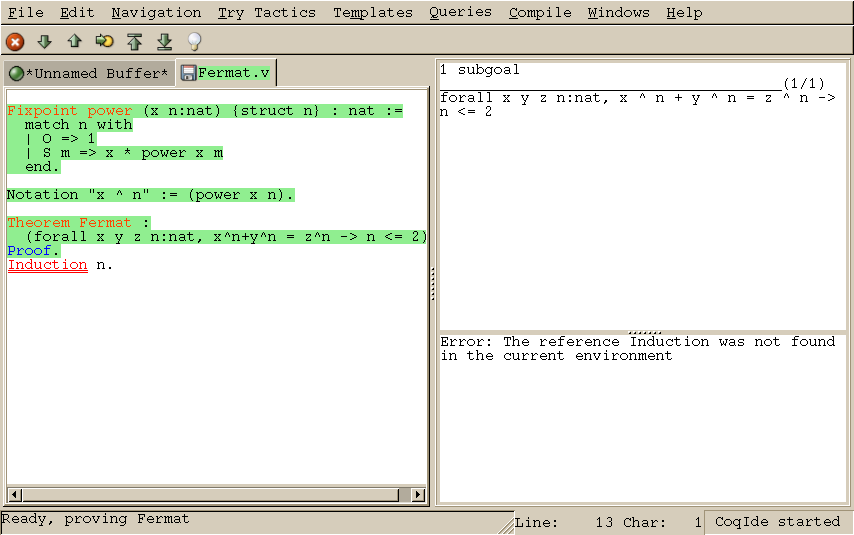
\includegraphics[width=1.0\textwidth]{coqide.png}
\else
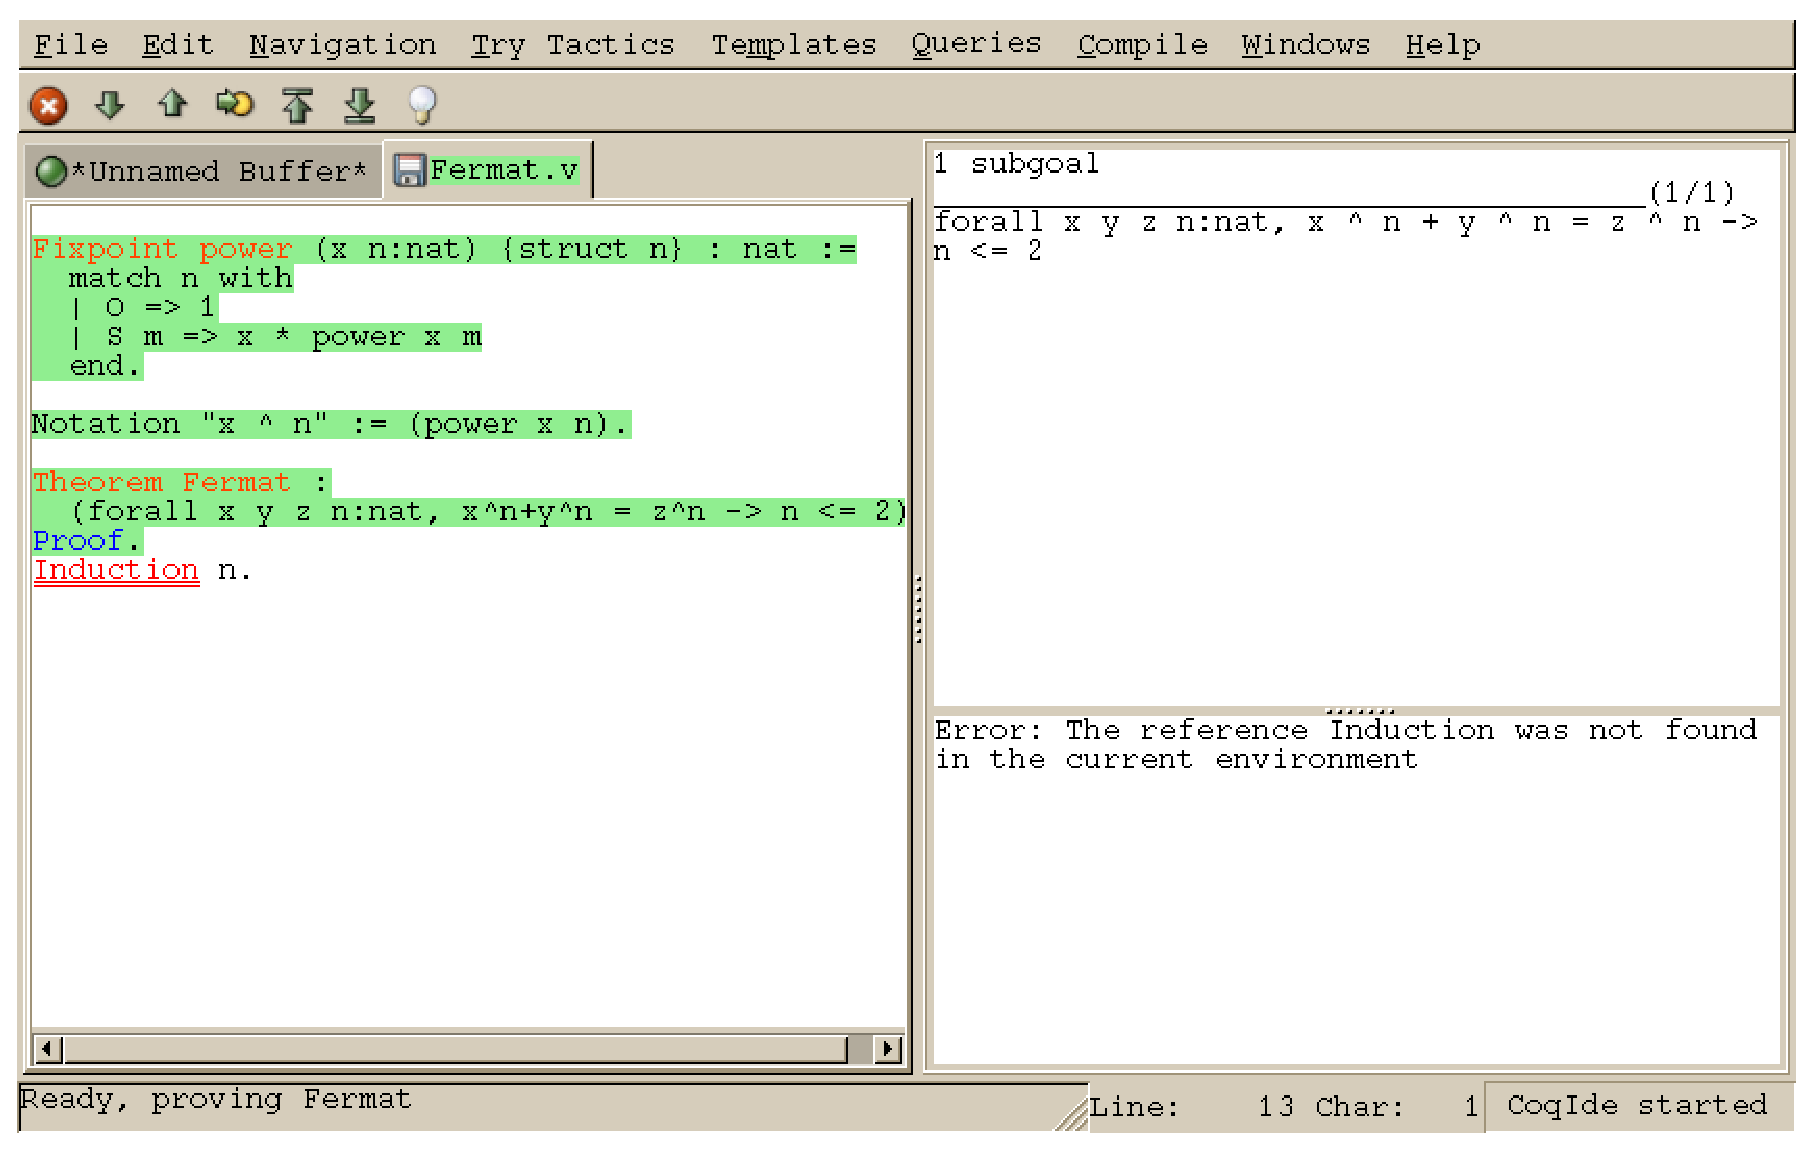
\includegraphics[width=1.0\textwidth]{coqide.eps}
\fi
%END LATEX
\end{center}
\caption{\CoqIDE{} main screen}
\label{fig:coqide}
\end{figure}

A sample \CoqIDE{} main screen, while navigating into a file
\verb|Fermat.v|, is shown on Figure~\ref{fig:coqide}.  At
the top is a menu bar, and a tool bar below it. The large window on
the left is displaying the various \emph{script buffers}. The upper right
window is the \emph{goal window}, where goals to 
prove are displayed. The lower right window is the \emph{message window},
where various messages resulting from commands are displayed. At the
bottom is the status bar.

\section{Managing files and buffers, basic edition}

In the script window, you may open arbitrarily many buffers to
edit. The \emph{File} menu allows you to open files or create some,
save them, print or export them into various formats. Among all these
buffers, there is always one which is the current \emph{running
  buffer}, whose name is displayed on a green background, which is the
one where Coq commands are currently executed. 

Buffers may be edited as in any text editor, and classical basic
editing commands (Copy/Paste, \ldots) are available in the \emph{Edit}
menu. \CoqIDE{} offers only basic editing commands, so if you need
more complex editing commands, you may launch your favorite text
editor on the current buffer, using the \emph{Edit/External Editor}
menu. 

\section{Interactive navigation into \Coq{} scripts}

The running buffer is the one where navigation takes place. The
toolbar proposes five basic commands for this. The first one,
represented by a down arrow icon, is for going forward executing one
command. If that command is successful, the part of the script that
has been executed is displayed on a green background. If that command
fails, the error message is displayed in the message window, and the
location of the error is emphasized by a red underline.

On Figure~\ref{fig:coqide}, the running buffer is \verb|Fermat.v|, all
commands until the \verb|Theorem| have been already executed, and the
user tried to go forward executing \verb|Induction n|. That command
failed because no such tactic exist (tactics are now in
lowercase\ldots), and the wrong word is underlined. 

Notice that the green part of the running buffer is not editable. If
you ever want to modify something you have to go backward using the up
arrow tool, or even better, put the cursor where you want to go back
and use the \textsf{goto} button. Unlike with \verb|coqtop|, you
should never use \verb|Undo| to go backward.

Two additional tool buttons exist, one to go directly to the end and
one to go back to the beginning. If you try to go to the end, or in
general to run several commands using the \textsf{goto} button, the
  execution will stop whenever an error is found.

If you ever try to execute a command which happens to run during a
long time, and would like to abort it before its
termination, you may use the interrupt button (the white cross on a red circle).
 
Finally, notice that these navigation buttons are also available in
the menu, where their keyboard shortcuts are given.

\section[Try tactics automatically]{Try tactics automatically\label{sec:trytactics}}

The menu \texttt{Try Tactics} provides some features for automatically
trying to solve the current goal using simple tactics. If such a
tactic succeeds in solving the goal, then its text is automatically
inserted into the script. There is finally a combination of these
tactics, called the \emph{proof wizard} which will try each of them in
turn. This wizard is also available as a tool button (the light
bulb).  The set of tactics tried by the wizard is customizable in
the preferences.

These tactics are general ones, in particular they do not refer to
particular hypotheses. You may also try specific tactics related to
the goal or one of the hypotheses, by clicking with the right mouse
button on the goal or the considered hypothesis. This is the
``contextual menu on goals'' feature, that may be disabled in the
preferences if undesirable.

\section{Proof folding}

As your script grows bigger and bigger, it might be useful to hide the proofs
of your theorems and lemmas.

This feature is toggled via the \texttt{Hide} entry of the \texttt{Navigation}
menu. The proof shall be enclosed between \texttt{Proof.} and \texttt{Qed.},
both with their final dots. The proof that shall be hidden or revealed is the
first one whose beginning statement (such as \texttt{Theorem}) precedes the
insertion cursor.
 
\section{Vernacular commands, templates}

The \texttt{Templates} menu allows using shortcuts to insert
vernacular commands. This is a nice way to proceed if you are not sure
of the spelling of the command you want.

Moreover, this menu offers some \emph{templates} which will automatic
insert a complex command like Fixpoint with a convenient shape for its
arguments. 

\section{Queries}

\begin{figure}[t]
\begin{center}
%HEVEA\imgsrc[alt="coqide query window"]{coqide-queries.png}
%BEGIN LATEX
\ifpdf  % si on est en pdflatex
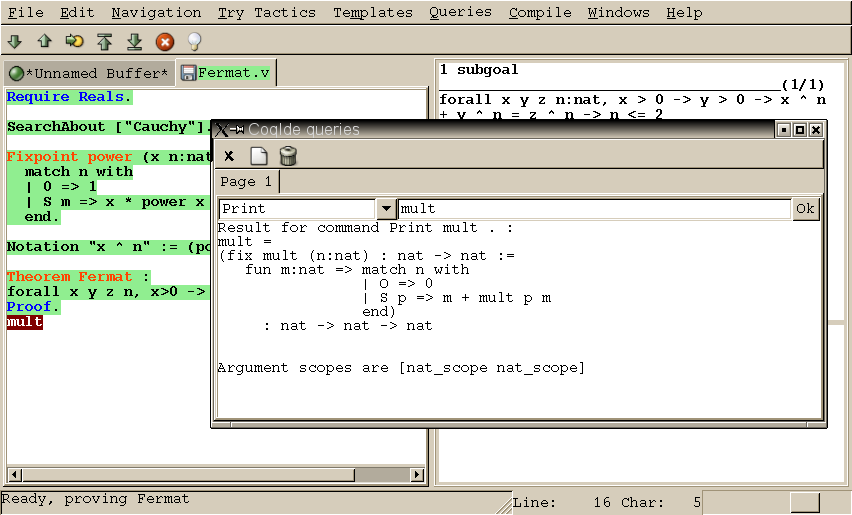
\includegraphics[width=1.0\textwidth]{coqide-queries.png}
\else
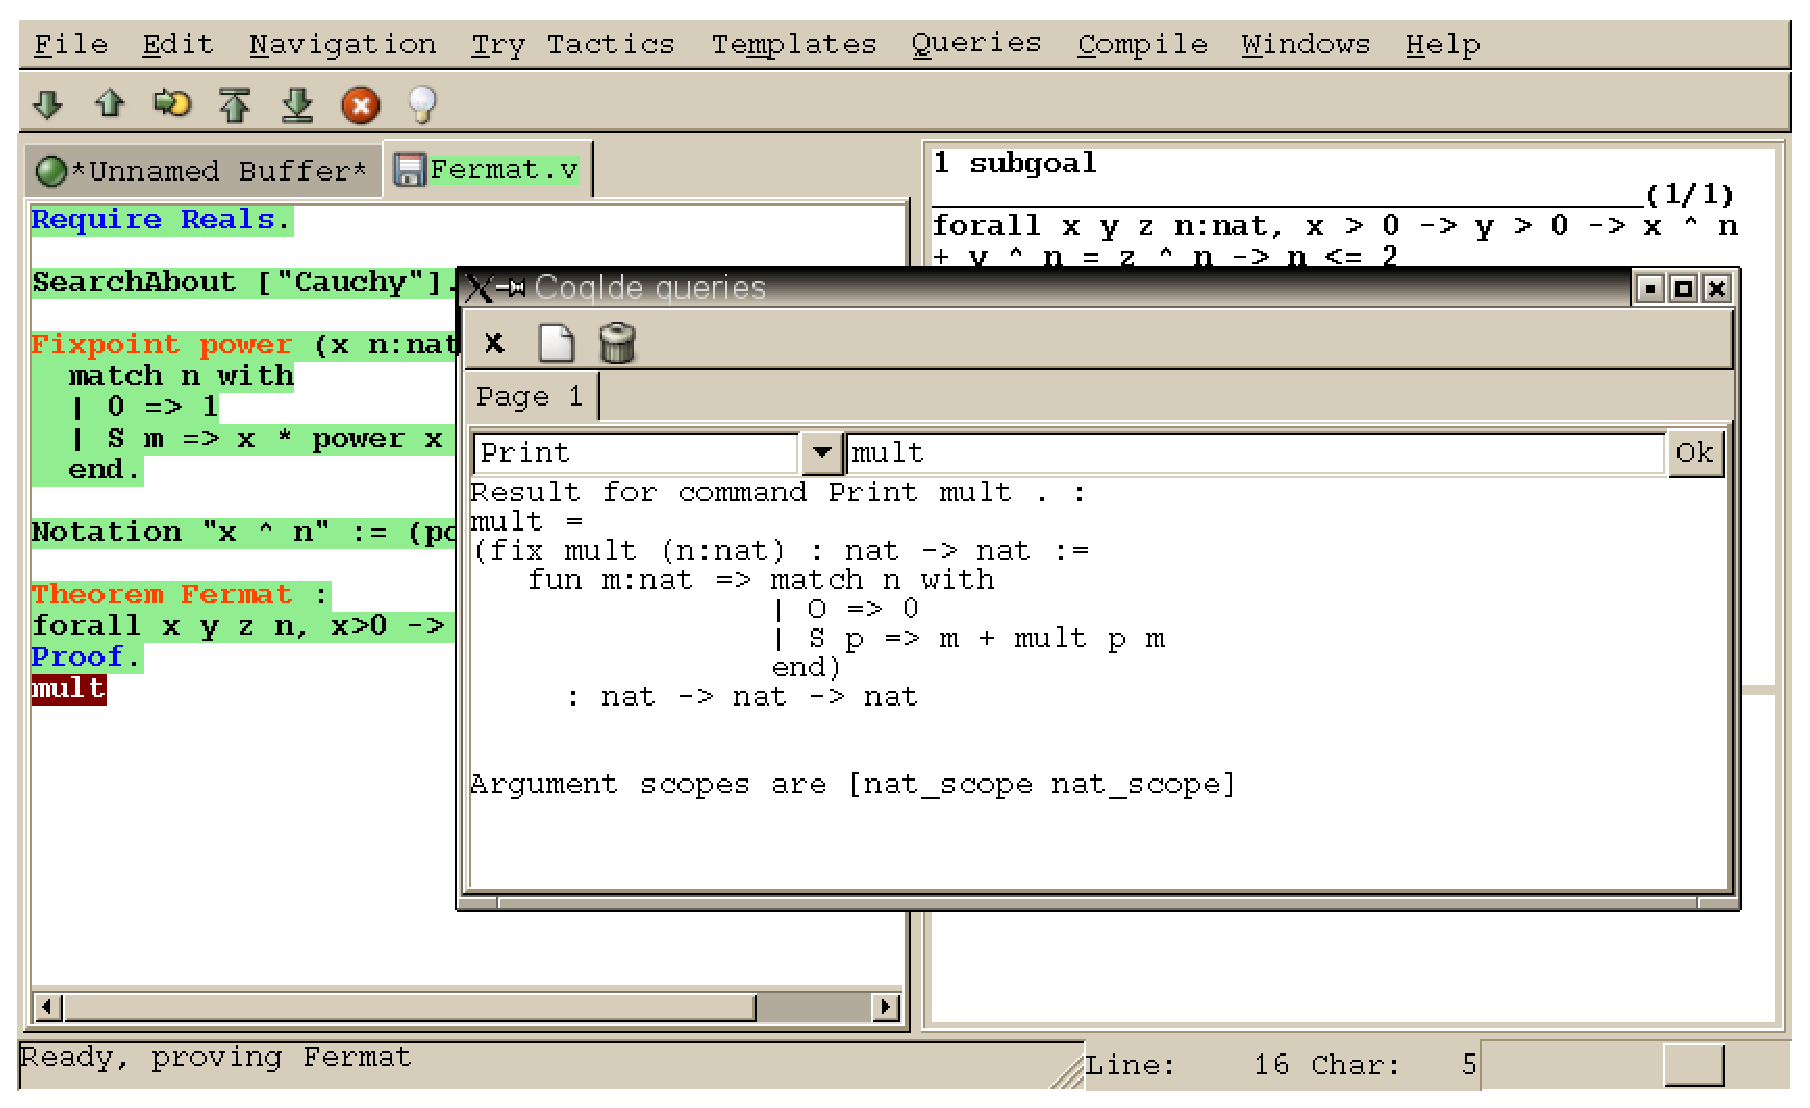
\includegraphics[width=1.0\textwidth]{coqide-queries.eps}
\fi
%END LATEX
\end{center}
\caption{\CoqIDE{}: the query window}
\label{fig:querywindow}
\end{figure}


We call \emph{query} any vernacular command that do not change the
current state, such as \verb|Check|, \verb|Search|, etc. Those
commands are of course useless during compilation of a file, hence
should not be included in scripts. To run such commands without
writing them in the script, \CoqIDE{} offers another input window
called the \emph{query window}. This window can be displayed on
demand, either by using the \texttt{Window} menu, or directly using
shortcuts given in the \texttt{Queries} menu. Indeed, with \CoqIDE{}
the simplest way to perform a \texttt{Search} on some identifier
is to select it using the mouse, and pressing \verb|F2|. This will
both make appear the query window and run the \texttt{Search} in
it, displaying the result. Shortcuts \verb|F3| and \verb|F4| are for
\verb|Check| and \verb|Print| respectively.
Figure~\ref{fig:querywindow} displays the query window after selection
of the word ``mult'' in the script windows, and pressing \verb|F4| to
print its definition.

\section{Compilation}

The \verb|Compile| menu offers direct commands to:
\begin{itemize}
\item compile the current buffer
\item run a compilation using \verb|make|
\item go to the last compilation error
\item create a \verb|makefile| using \verb|coq_makefile|.
\end{itemize}

\section{Customizations}

You may customize your environment using menu
\texttt{Edit/Preferences}. A new window will be displayed, with
several customization sections presented as a notebook. 

The first section is for selecting the text font used for scripts, goal
and message windows. 

The second section is devoted to file management: you may
configure automatic saving of files, by periodically saving the
contents into files named \verb|#f#| for each opened file
\verb|f|. You may also activate the \emph{revert} feature: in case a
opened file is modified on the disk by a third party, \CoqIDE{} may read
it again for you. Note that in the case you edited that same file, you
will be prompt to choose to either discard your changes or not. The
\texttt{File charset encoding} choice is described below in
Section~\ref{sec:coqidecharencoding}
 

The \verb|Externals| section allows customizing the external commands
for compilation, printing, web browsing. In the browser command, you
may use \verb|%s| to denote the URL to open, for example: %
\verb|mozilla -remote "OpenURL(%s)"|. 

The \verb|Tactics Wizard| section allows defining the set of tactics
that should be tried, in sequence, to solve the current goal.

The last section is for miscellaneous boolean settings, such as the
``contextual menu on goals'' feature presented in
Section~\ref{sec:trytactics}. 

Notice that these settings are saved in the file \verb|.coqiderc| of
your home directory. 

A gtk2 accelerator keymap is saved under the name \verb|.coqide.keys|.
It is not recommanded to edit this file manually: to modify a given menu
shortcut, go to the corresponding menu item without releasing the
mouse button, press the key you want for the new shortcut, and release
the mouse button afterwards. If your system does not allow it, you may still 
edit this configuration file by hand, but this is more involved.

\section{Using Unicode symbols}

\CoqIDE{} is based on GTK+ and inherits from it support for Unicode in
its text windows. Consequently a large set of symbols is available for
notations.

\subsection{Displaying Unicode symbols}

You just need to define suitable notations as described in
Chapter~\ref{Addoc-syntax}. For example, to use the mathematical symbols
$\forall$ and $\exists$, you may define 
\begin{quote}\tt
Notation "$\forall$ x : t, P" := \\
\qquad  (forall x:t, P) (at level 200, x ident).\\
Notation "$\exists$ x : t, P" := \\
\qquad  (exists x:t, P) (at level 200, x ident).
\end{quote}
There exists a small set of such notations already defined, in the
file \verb|utf8.v| of \Coq{} library, so you may enable them just by 
\verb|Require utf8| inside \CoqIDE{}, or equivalently, by starting
\CoqIDE{} with \verb|coqide -l utf8|.

However, there are some issues when using such Unicode symbols: you of
course need to use a character font which supports them. In the Fonts
section of the preferences, the Preview line displays some Unicode symbols, so
you could figure out if the selected font is OK. Related to this, one
thing you may need to do is choose whether GTK+ should use antialiased
fonts or not, by setting the environment variable \verb|GDK_USE_XFT|
to 1 or 0 respectively.

\subsection{Defining an input method for non ASCII symbols}

To input a Unicode symbol, a general method provided by GTK+
is to simultaneously press the
Control, Shift and ``u'' keys, release, then type the hexadecimal code of the
symbol required, for example \verb|2200| for the $\forall$ symbol.
A list of symbol codes is available at \url{http://www.unicode.org}. 

An alternative method which does not require to know the hexadecimal
code of the character is to use an Input Method Editor. On POSIX
systems (Linux distributions, BSD variants and MacOS X), you can use
\texttt{uim} version 1.6 or later which provides a \LaTeX{}-style
input method.

To configure \texttt{uim}, execute \texttt{uim-pref-gtk} as your regular user.
In the "Global Settings" group set the default Input Method to "ELatin" (don't
forget to tick the checkbox "Specify default IM"). In the "ELatin" group set the
layout to "TeX", and remember the content of the "[ELatin] on" field (by default
Control-\textbackslash). You can now execute CoqIDE with the following commands (assuming
you use a Bourne-style shell):

\begin{verbatim}
$ export GTK_IM_MODULE=uim
$ coqide
\end{verbatim}

Activate the ELatin Input Method with Control-\textbackslash, then type the
sequence "\verb=\Gamma=". You will see the sequence being
replaced by $\Gamma$ as soon as you type the second "a".

\subsection[Character encoding for saved files]{Character encoding for saved files\label{sec:coqidecharencoding}}

In the \texttt{Files} section of the preferences, the encoding option
is related to the way files are saved. 

If you have no need to exchange files with non UTF-8 aware
applications, it is better to choose the UTF-8 encoding, since it
guarantees that your files will be read again without problems. (This
is because when \CoqIDE{} reads a file, it tries to automatically
detect its character encoding.) 

If you choose something else than UTF-8, then missing characters will
be written encoded by \verb|\x{....}| or \verb|\x{........}| where
each dot is an hexadecimal digit: the number between braces is the
hexadecimal Unicode index for the missing character.


%%% Local Variables: 
%%% mode: latex
%%% TeX-master: "Reference-Manual"
%%% End: 
% Coq IDE

%BEGIN LATEX
\RefManCutCommand{BEGINADDENDUM=\thepage}
%END LATEX
\part{Addendum to the Reference Manual}
%\coverpage{Addendum to the Reference Manual}{\ }
%\addcontentsline{toc}{part}{Additional documentation}
%BEGIN LATEX
\setheaders{Presentation of the Addendum}
%END LATEX
\chapter*{Presentation of the Addendum}
%HEVEA\cutname{addendum.html}

Here you will find several pieces of additional documentation for the
\Coq\ Reference Manual. Each of this chapters is concentrated on a
particular topic, that should interest only a fraction of the \Coq\
users: that's the reason why they are apart from the Reference
Manual.

\begin{description}

\item[Extended pattern-matching] This chapter details the use of
  generalized pattern-matching. It is contributed by Cristina Cornes
  and Hugo Herbelin.

\item[Implicit coercions] This chapter details the use of the coercion
  mechanism.  It is contributed by Amokrane Saïbi.

%\item[Proof of imperative programs] This chapter explains how to
%  prove properties of annotated programs with imperative features.
%  It is contributed by Jean-Christophe Filliâtre

\item[Program extraction] This chapter explains how to extract in practice ML
  files from $\FW$ terms.   It is contributed by Jean-Christophe
  Filliâtre and Pierre Letouzey.

\item[Program] This chapter explains the use of the \texttt{Program}
  vernacular which allows the development of certified
  programs in \Coq. It is contributed by Matthieu Sozeau and replaces
  the previous \texttt{Program} tactic by Catherine Parent.

%\item[Natural] This chapter is due to Yann Coscoy. It is the user
%  manual of the tools he wrote for printing proofs in natural
%  language. At this time, French and English languages are supported.

\item[omega] \texttt{omega}, written by Pierre Crégut, solves a whole
  class of arithmetic problems.

\item[The {\tt ring} tactic] This is a tactic to do AC rewriting. This
  chapter explains how to use it and how it works.
  The chapter is contributed by Patrick Loiseleur.

\item[The {\tt Setoid\_replace} tactic] This is a
  tactic to do rewriting on types equipped with specific (only partially
  substitutive) equality. The chapter is contributed by Clément Renard.

\item[Calling external provers] This chapter describes several tactics
  which call external provers.

\end{description}

\atableofcontents


%%% Local Variables: 
%%% mode: latex
%%% TeX-master: "Reference-Manual"
%%% End: 
%
\achapter{Extended pattern-matching}
%BEGIN LATEX
\defaultheaders
%END LATEX
\aauthor{Cristina Cornes and Hugo Herbelin}

\label{Mult-match-full}
\ttindex{Cases}
\index{ML-like patterns}

This section describes the full form of pattern-matching in {\Coq} terms.

\asection{Patterns}\label{implementation} The full syntax of {\tt
match} is presented in Figures~\ref{term-syntax}
and~\ref{term-syntax-aux}.  Identifiers in patterns are either
constructor names or variables. Any identifier that is not the
constructor of an inductive or coinductive type is considered to be a
variable. A variable name cannot occur more than once in a given
pattern. It is recommended to start variable names by a lowercase
letter.

If a pattern has the form $(c~\vec{x})$ where $c$ is a constructor
symbol and $\vec{x}$ is a linear vector of (distinct) variables, it is
called {\em simple}: it is the kind of pattern recognized by the basic
version of {\tt match}. On the opposite, if it is a variable $x$ or
has the form $(c~\vec{p})$ with $p$ not only made of variables, the
pattern is called {\em nested}.

A variable pattern matches any value, and the identifier is bound to
that value. The pattern ``\texttt{\_}'' (called ``don't care'' or
``wildcard'' symbol) also matches any value, but does not bind
anything. It may occur an arbitrary number of times in a
pattern. Alias patterns written \texttt{(}{\sl pattern} \texttt{as}
{\sl identifier}\texttt{)} are also accepted. This pattern matches the
same values as {\sl pattern} does and {\sl identifier} is bound to the
matched value.  
A pattern of the form {\pattern}{\tt |}{\pattern} is called
disjunctive. A list of patterns separated with commas is also
considered as a pattern and is called {\em multiple pattern}. However
multiple patterns can only occur at the root of pattern-matching
equations. Disjunctions of {\em multiple pattern} are allowed though.

Since extended {\tt match} expressions are compiled into the primitive
ones, the expressiveness of the theory remains the same. Once the
stage of parsing has finished only simple patterns remain.  Re-nesting
of pattern is performed at printing time. An easy way to see the
result of the expansion is to toggle off the nesting performed at
printing (use here {\tt Set Printing Matching}), then by printing the term
with \texttt{Print} if the term is a constant, or using the command
\texttt{Check}.

The extended \texttt{match} still accepts an optional {\em elimination
predicate} given after the keyword \texttt{return}.  Given a pattern
matching expression, if all the right-hand-sides of \texttt{=>} ({\em
rhs} in short) have the same type, then this type can be sometimes
synthesized, and so we can omit the \texttt{return} part. Otherwise 
the predicate after \texttt{return} has to be provided, like for the basic
\texttt{match}.

Let us illustrate through examples the different aspects of extended
pattern matching. Consider for example the function that computes the
maximum of two natural numbers. We can write it in primitive syntax
by:

\begin{coq_example}
Fixpoint max (n m:nat) {struct m} : nat :=
  match n with
  | O => m
  | S n' => match m with
            | O => S n'
            | S m' => S (max n' m')
            end
  end.
\end{coq_example}

\paragraph{Multiple patterns}

Using multiple patterns in the definition of {\tt max} allows to write:

\begin{coq_example}
Reset max.
Fixpoint max (n m:nat) {struct m} : nat :=
  match n, m with
  | O, _ => m
  | S n', O => S n'
  | S n', S m' => S (max n' m')
  end.
\end{coq_example}

which will be compiled into the previous form.

The pattern-matching compilation strategy examines patterns from left
to right. A \texttt{match} expression is generated {\bf only} when
there is at least one constructor in the column of patterns. E.g. the
following example does not build a \texttt{match} expression.

\begin{coq_example}
Check (fun x:nat => match x return nat with
                    | y => y
                    end).
\end{coq_example}

\paragraph{Aliasing subpatterns}

We can also use ``\texttt{as} {\ident}'' to associate a name to a
sub-pattern:

\begin{coq_example}
Reset max.
Fixpoint max (n m:nat) {struct n} : nat :=
  match n, m with
  | O, _ => m
  | S n' as p, O => p
  | S n', S m' => S (max n' m')
  end.
\end{coq_example}

\paragraph{Nested patterns}

Here is now an example of nested patterns:

\begin{coq_example}
Fixpoint even (n:nat) : bool :=
  match n with
  | O => true
  | S O => false
  | S (S n') => even n'
  end.
\end{coq_example}

This is compiled into:

\begin{coq_example}
Print even.
\end{coq_example}

In the previous examples patterns do not conflict with, but
sometimes it is comfortable to write patterns that admit a non
trivial superposition. Consider
the boolean function \texttt{lef} that given two natural numbers
yields \texttt{true} if the first one is less or equal than the second
one and \texttt{false} otherwise. We can write it as follows:

\begin{coq_example}
Fixpoint lef (n m:nat) {struct m} : bool :=
  match n, m with
  | O, x => true
  | x, O => false
  | S n, S m => lef n m
  end.
\end{coq_example}

Note that the first and the second multiple pattern superpose because
the couple of values \texttt{O O} matches both. Thus, what is the result
of the function on those values?  To eliminate ambiguity we use the
{\em textual priority rule}: we consider patterns ordered from top to
bottom, then a value is matched by the pattern at the $ith$ row if and
only if it is not matched by some pattern of a previous row. Thus in the
example,
\texttt{O O} is matched by the first pattern, and so \texttt{(lef O O)}
yields \texttt{true}.

Another way to write  this function is:

\begin{coq_example}
Reset lef.
Fixpoint lef (n m:nat) {struct m} : bool :=
  match n, m with
  | O, x => true
  | S n, S m => lef n m
  | _, _ => false
  end.
\end{coq_example}

Here the last pattern superposes with the first two. Because
of the priority rule, the last pattern 
will be used only for values that do not match neither the  first nor
the second one.  

Terms with useless patterns are not accepted by the
system. Here is an example:
% Test failure
\begin{coq_eval}
Set Printing Depth 50.
  (********** The following is not correct and should produce **********)
  (**************** Error: This clause is redundant ********************)
\end{coq_eval}
\begin{coq_example}
Check (fun x:nat =>
         match x with
         | O => true
         | S _ => false
         | x => true
         end).
\end{coq_example}

\paragraph{Disjunctive patterns}

Multiple patterns that share the same right-hand-side can be
factorized using the notation \nelist{\multpattern}{\tt |}. For instance,
{\tt max} can be rewritten as follows:

\begin{coq_eval}
Reset max.
\end{coq_eval}
\begin{coq_example}
Fixpoint max (n m:nat) {struct m} : nat :=
  match n, m with
  | S n', S m' => S (max n' m')
  | 0, p | p, 0 => p
  end.
\end{coq_example}

Similarly, factorization of (non necessary multiple) patterns
that share the same variables is possible by using the notation
\nelist{\pattern}{\tt |}. Here is an example:

\begin{coq_example}
Definition filter_2_4 (n:nat) : nat :=
  match n with
  | 2 as m | 4 as m => m
  | _ => 0
  end.
\end{coq_example}

Here is another example using disjunctive subpatterns.

\begin{coq_example}
Definition filter_some_square_corners (p:nat*nat) : nat*nat :=
  match p with
  | ((2 as m | 4 as m), (3 as n | 5 as n)) => (m,n)
  | _ => (0,0)
  end.
\end{coq_example}

\asection{About patterns of parametric types}
When matching objects of a parametric type, constructors in patterns
{\em do not expect} the parameter arguments. Their value is deduced
during expansion.
Consider for example the type of polymorphic lists:

\begin{coq_example}
Inductive List (A:Set) : Set :=
  | nil : List A
  | cons : A -> List A -> List A.
\end{coq_example}

We can check the function {\em tail}:

\begin{coq_example}
Check
  (fun l:List nat =>
     match l with
     | nil => nil nat
     | cons _ l' => l'
     end).
\end{coq_example}


When we use parameters in patterns there is an error message:
% Test failure
\begin{coq_eval}
Set Printing Depth 50.
(********** The following is not correct and should produce **********)
(******** Error: The constructor cons expects 2 arguments ************)
\end{coq_eval}
\begin{coq_example}
Check
  (fun l:List nat =>
     match l with
     | nil A => nil nat
     | cons A _ l' => l'
     end).
\end{coq_example}



\asection{Matching objects of dependent types}
The previous examples illustrate pattern matching on objects of
non-dependent types, but we can also 
use the expansion strategy to destructure objects of dependent type.
Consider the type \texttt{listn} of lists of a certain length:
\label{listn}

\begin{coq_example}
Inductive listn : nat -> Set :=
  | niln : listn 0
  | consn : forall n:nat, nat -> listn n -> listn (S n).
\end{coq_example}

\asubsection{Understanding dependencies in patterns}
We can define the function \texttt{length} over \texttt{listn} by:

\begin{coq_example}
Definition length (n:nat) (l:listn n) := n.
\end{coq_example}

Just for illustrating pattern matching, 
we can define it by case analysis:

\begin{coq_example}
Reset length.
Definition length (n:nat) (l:listn n) :=
  match l with
  | niln => 0
  | consn n _ _ => S n
  end.
\end{coq_example}

We can understand the meaning of this definition using the
same notions of usual pattern matching.

%
% Constraining of dependencies is not longer valid in V7
%
\iffalse
Now suppose we split the second pattern  of \texttt{length} into two 
cases so to give an
alternative definition using nested patterns:
\begin{coq_example}
Definition length1 (n:nat) (l:listn n) :=
  match l with
  | niln => 0
  | consn n _ niln => S n
  | consn n _ (consn _ _ _) => S n
  end.
\end{coq_example}

It is obvious that \texttt{length1} is  another version of
\texttt{length}. We can also give the following definition:
\begin{coq_example}
Definition length2 (n:nat) (l:listn n) :=
  match l with
  | niln => 0
  | consn n _ niln => 1
  | consn n _ (consn m _ _) => S (S m)
  end.
\end{coq_example}

If we forget that \texttt{listn} is a dependent type and we read these
definitions using the usual semantics of pattern matching,  we can conclude
that \texttt{length1}
and \texttt{length2} are different functions.
In fact, they are equivalent
because the pattern \texttt{niln} implies that \texttt{n} can only match
the value $0$ and analogously the pattern \texttt{consn} determines that \texttt{n} can
only match  values of the form  $(S~v)$ where $v$ is the value matched by
\texttt{m}. 

The converse is also true. If
we destructure the  length  value with the pattern \texttt{O} then the list
value should be $niln$. 
Thus, the following term \texttt{length3} corresponds to the function
\texttt{length} but this time defined by case analysis on the dependencies instead of on the list:

\begin{coq_example}
Definition length3 (n:nat) (l:listn n) :=
  match l with
  | niln => 0
  | consn O _ _ => 1
  | consn (S n) _ _ => S (S n)
  end.
\end{coq_example}

When we have nested patterns of dependent types, the semantics of
pattern matching becomes a little more difficult because
the set of values that are matched by a sub-pattern may be conditioned by the
values matched by another sub-pattern. Dependent nested patterns are
somehow constrained patterns. 
In the examples, the expansion of
\texttt{length1} and \texttt{length2} yields exactly the same term
 but the
expansion of \texttt{length3} is completely different. \texttt{length1} and
\texttt{length2} are expanded into two nested case analysis on
\texttt{listn} while \texttt{length3} is expanded into a case analysis on
\texttt{listn} containing a case analysis on natural numbers inside.


In practice the user can think about the patterns as independent and
it is the expansion algorithm that cares to relate them. \\
\fi
%
%
%

\asubsection{When the elimination predicate must be provided}
The examples  given so far do not need an explicit elimination predicate
 because all the rhs have the same type and the
strategy succeeds to synthesize it.
Unfortunately when dealing with dependent patterns it often happens
that we need to write cases where the type of the rhs are 
different  instances of the elimination  predicate.
The function  \texttt{concat} for \texttt{listn}
is an example where the branches have different type
and we need to provide the elimination predicate:

\begin{coq_example}
Fixpoint concat (n:nat) (l:listn n) (m:nat) (l':listn m) {struct l} :
 listn (n + m) :=
  match l in listn n return listn (n + m) with
  | niln => l'
  | consn n' a y => consn (n' + m) a (concat n' y m l')
  end.
\end{coq_example}
The elimination predicate is {\tt fun (n:nat) (l:listn n) => listn~(n+m)}.
In general if $m$ has type $(I~q_1\ldots q_r~t_1\ldots t_s)$ where 
$q_1\ldots q_r$ are parameters, the elimination predicate should be of
the form~:
{\tt fun $y_1$\ldots $y_s$ $x$:($I$~$q_1$\ldots $q_r$~$y_1$\ldots
  $y_s$) => P}. 

In the concrete syntax, it should be written~:
\[ \kw{match}~m~\kw{as}~x~\kw{in}~(I~\_\ldots \_~y_1\ldots y_s)~\kw{return}~Q~\kw{with}~\ldots~\kw{end}\]

The variables which appear in the \kw{in} and \kw{as} clause are new
and bounded in the property $Q$ in the \kw{return} clause. The
parameters of the inductive definitions should not be mentioned and
are replaced by \kw{\_}.

Recall that a list of patterns is also a pattern. So, when
we destructure several terms at the same time and the branches have
different type  we need to provide
the elimination predicate for this multiple pattern. 
It is done using the same scheme, each term may be associated to an
\kw{as} and \kw{in} clause in order to introduce a dependent product.

For example, an equivalent definition for \texttt{concat} (even though the matching on the second term is trivial) would have
been:

\begin{coq_example}
Reset concat.
Fixpoint concat (n:nat) (l:listn n) (m:nat) (l':listn m) {struct l} :
 listn (n + m) :=
  match l in listn n, l' return listn (n + m) with
  | niln, x => x
  | consn n' a y, x => consn (n' + m) a (concat n' y m x)
  end.
\end{coq_example}

% Notice that this time, the predicate \texttt{[n,\_:nat](listn (plus n
%   m))}  is binary because we
% destructure both \texttt{l} and \texttt{l'} whose types have arity one.
% In general, if we destructure the terms $e_1\ldots e_n$
% the predicate will be of arity $m$ where $m$ is the sum of the
% number of dependencies of the type of $e_1, e_2,\ldots e_n$ 
% (the $\lambda$-abstractions
% should correspond from left to right to each dependent argument of the
% type of $e_1\ldots e_n$).
When the arity of the predicate (i.e. number of abstractions) is not
correct Coq raises an error message. For example:

% Test failure
\begin{coq_eval}
Reset concat.
Set Printing Depth 50.
(********** The following is not correct and should produce ***********)
(** Error: the term l' has type listn m while it is expected to have **)
(** type listn (?31 + ?32)                                           **)
\end{coq_eval}
\begin{coq_example}
Fixpoint concat
 (n:nat) (l:listn n) (m:nat)
 (l':listn m) {struct l} : listn (n + m) :=
  match l, l' with
  | niln, x => x
  | consn n' a y, x => consn (n' + m) a (concat n' y m x)
  end.
\end{coq_example}

\asection{Using pattern matching to write proofs}
In all the previous examples the elimination predicate does not depend
on the object(s) matched. But it may depend and the typical case 
is when we write a proof by induction or a function that yields an
object of dependent type. An example of proof using \texttt{match} in
given in Section~\ref{refine-example}

For example, we can write 
the function \texttt{buildlist} that given a natural number
$n$ builds a list of length $n$ containing zeros as follows:

\begin{coq_example}
Fixpoint buildlist (n:nat) : listn n :=
  match n return listn n with
  | O => niln
  | S n => consn n 0 (buildlist n)
  end.
\end{coq_example}

We can also use multiple patterns. 
Consider the following definition of the predicate less-equal
\texttt{Le}:

\begin{coq_example}
Inductive LE : nat -> nat -> Prop :=
  | LEO : forall n:nat, LE 0 n
  | LES : forall n m:nat, LE n m -> LE (S n) (S m).
\end{coq_example}

We can use multiple patterns to write  the proof of the lemma
 \texttt{forall (n m:nat), (LE n m)}\verb=\/=\texttt{(LE m n)}:

\begin{coq_example}
Fixpoint dec (n m:nat) {struct n} : LE n m \/ LE m n :=
  match n, m return LE n m \/ LE m n with
  | O, x => or_introl (LE x 0) (LEO x)
  | x, O => or_intror (LE x 0) (LEO x)
  | S n as n', S m as m' =>
      match dec n m with
      | or_introl h => or_introl (LE m' n') (LES n m h)
      | or_intror h => or_intror (LE n' m') (LES m n h)
      end
  end.
\end{coq_example}
In the example of \texttt{dec},
the first \texttt{match} is dependent while 
the second is not.

% In general, consider the terms $e_1\ldots e_n$,
% where  the type of $e_i$ is an instance of a family type
% $\lb (\vec{d_i}:\vec{D_i}) \mto T_i$  ($1\leq i
% \leq n$). Then, in expression \texttt{match}  $e_1,\ldots,
% e_n$ \texttt{of} \ldots \texttt{end}, the 
% elimination predicate ${\cal P}$ should be of the form:
% $[\vec{d_1}:\vec{D_1}][x_1:T_1]\ldots [\vec{d_n}:\vec{D_n}][x_n:T_n]Q.$

The user can also use \texttt{match} in combination with the tactic
\texttt{refine} (see Section~\ref{refine}) to build incomplete proofs
beginning with a \texttt{match} construction.

\asection{Pattern-matching on inductive objects involving local
definitions}

If local definitions occur in the type of a constructor, then there
are two ways to match on this constructor. Either the local
definitions are skipped and matching is done only on the true arguments
of the constructors, or the bindings for local definitions can also
be caught in the matching.

Example.

\begin{coq_eval}
Reset Initial.
Require Import Arith.
\end{coq_eval}

\begin{coq_example*}
Inductive list : nat -> Set :=
  | nil : list 0
  | cons : forall n:nat, let m := (2 * n) in list m -> list (S (S m)).
\end{coq_example*}

In the next example, the local definition is not caught.

\begin{coq_example}
Fixpoint length n (l:list n) {struct l} : nat :=
  match l with
  | nil => 0
  | cons n l0 => S (length (2 * n) l0)
  end.
\end{coq_example}

But in this example, it is.

\begin{coq_example}
Fixpoint length' n (l:list n) {struct l} : nat :=
  match l with
  | nil => 0
  | cons _ m l0 => S (length' m l0)
  end.
\end{coq_example}

\Rem for a given matching clause, either none of the local
definitions or all of them can be caught.

\asection{Pattern-matching and coercions}

If a mismatch occurs between the expected type of a pattern and its
actual type, a coercion made from constructors is sought. If such a
coercion can be found, it is automatically inserted around the
pattern.

Example:

\begin{coq_example}
Inductive I : Set :=
  | C1 : nat -> I
  | C2 : I -> I.
Coercion C1 : nat >-> I.
Check (fun x => match x with
                | C2 O => 0
                | _ => 0
                end).
\end{coq_example}


\asection{When does the expansion strategy fail ?}\label{limitations}
The strategy works very like in ML languages when treating
patterns of non-dependent type.  
But there are new cases of failure that are due to the presence of 
dependencies. 

The error messages of the current implementation may be sometimes
confusing.  When the tactic fails because patterns are somehow
incorrect then error messages refer to the initial expression. But the
strategy may succeed to build an expression whose sub-expressions are
well typed when the whole expression is not. In this situation the
message makes reference to the expanded expression.  We encourage
users, when they have patterns with the same outer constructor in
different equations, to name the variable patterns in the same
positions with the same name.  
E.g. to write {\small\texttt{(cons n O x) => e1}} 
and {\small\texttt{(cons n \_ x) => e2}} instead of
{\small\texttt{(cons n O x) => e1}} and 
{\small\texttt{(cons n' \_ x') => e2}}. 
This helps to maintain certain name correspondence between the
generated expression and the original.

Here is a summary of the error messages corresponding to each situation:

\begin{ErrMsgs}
\item \sverb{The constructor } {\sl
    ident} \sverb{expects } {\sl num} \sverb{arguments}
  
 \sverb{The variable } {\sl ident} \sverb{is bound several times
    in pattern } {\sl term}
  
 \sverb{Found a constructor of inductive type} {\term}
 \sverb{while a constructor of} {\term} \sverb{is expected}

 Patterns are incorrect (because constructors are not applied to
  the correct number of the arguments, because they are not linear or
  they are wrongly typed)

\item \errindex{Non exhaustive pattern-matching}

the pattern matching is not exhaustive

\item \sverb{The elimination predicate } {\sl term} \sverb{should be
    of arity } {\sl num} \sverb{(for non dependent case) or } {\sl
    num} \sverb{(for dependent case)}

The elimination predicate provided to \texttt{match} has not the
  expected arity


%\item the whole expression is wrongly typed

% CADUC ?
% , or the synthesis of
%   implicit arguments fails (for example to find the elimination
%   predicate or to resolve implicit arguments in the rhs).
 
%   There are {\em nested patterns of dependent type}, the elimination
%   predicate corresponds to non-dependent case and has the form
%   $[x_1:T_1]...[x_n:T_n]T$ and {\bf some} $x_i$ occurs {\bf free} in
%   $T$.  Then, the strategy may fail to find out a correct elimination
%   predicate during some step of compilation.  In this situation we
%   recommend the user to rewrite the nested dependent patterns into
%   several \texttt{match} with {\em simple patterns}.
  
\item {\tt Unable to infer a match predicate\\
    Either there is a type incompatiblity or the problem involves\\
    dependencies}
 
  There is a type mismatch between the different branches

  Then the user should provide an elimination predicate.

% Obsolete ?  
% \item because of nested patterns, it may happen that even though all
%   the rhs have the same type, the strategy needs dependent elimination
%   and so an elimination predicate must be provided. The system warns
%   about this situation, trying to compile anyway with the
%   non-dependent strategy. The risen message is:

% \begin{itemize}
% \item {\tt Warning: This pattern matching may need dependent
%     elimination to be compiled.  I will try, but if fails try again
%     giving dependent elimination predicate.}
% \end{itemize}


%%%%%%%%%%%%%%%%%%%%%%%%%%%%%%%%%%%%%%%%%%%%%%%%%%%%%%%%%%%%%%%%%%%%%%
% % LA PROPAGATION DES CONTRAINTES ARRIERE N'EST PAS FAITE DANS LA V7
% TODO
% \item there are {\em nested patterns of dependent type} and the
%   strategy builds a term that is well typed but recursive calls in fix
%   point are reported as illegal:
% \begin{itemize}
% \item {\tt Error: Recursive call applied to an illegal term ...}
% \end{itemize}

% This is because the strategy generates a term that is correct w.r.t.
% the initial term but which does not pass the guard condition.  In
% this situation we recommend the user to transform the nested dependent
% patterns into {\em several \texttt{match} of simple patterns}.  Let us
% explain this with an example.  Consider the following definition of a
% function that yields the last element of a list and \texttt{O} if it is
% empty:

% \begin{coq_example}
%   Fixpoint last [n:nat; l:(listn n)] : nat :=
%    match l of 
%      (consn _ a niln) => a
%    | (consn m _ x) => (last m x) | niln => O
%    end.
% \end{coq_example}

% It fails because of the priority between patterns, we know that this
% definition is equivalent to the following more explicit one (which
% fails too):

% \begin{coq_example*}
%   Fixpoint last [n:nat; l:(listn n)] : nat :=
%    match l of
%      (consn _ a niln) => a
%    | (consn n _ (consn m b x)) => (last n (consn m b x))
%    | niln => O
%    end.
% \end{coq_example*}

% Note that the recursive call {\tt (last n (consn m b x))} is not
% guarded. When treating with patterns of dependent types the strategy
% interprets the first definition of \texttt{last} as the second
% one\footnote{In languages of the ML family the first definition would
%   be translated into a term where the variable \texttt{x} is shared in
%   the expression.  When patterns are of non-dependent types, Coq
%   compiles as in ML languages using sharing. When patterns are of
%   dependent types the compilation reconstructs the term as in the
%   second definition of \texttt{last} so to ensure the result of
%   expansion is well typed.}.  Thus it generates a term where the
% recursive call is rejected by the guard condition.

% You can get rid of this problem by writing the definition with
% \emph{simple patterns}:

% \begin{coq_example}
%   Fixpoint last [n:nat; l:(listn n)] : nat :=
%   <[_:nat]nat>match l of
%     (consn m a x) => Cases x of niln => a | _ => (last m x) end
%   | niln => O
%   end.
% \end{coq_example}

\end{ErrMsgs}


%%% Local Variables: 
%%% mode: latex
%%% TeX-master: "Reference-Manual"
%%% End: 
%
\achapter{Implicit Coercions}
\aauthor{Amokrane Saïbi}

\label{Coercions-full}
\index{Coercions!presentation}

\asection{General Presentation}

This section describes the inheritance mechanism of {\Coq}. In {\Coq} with
inheritance, we are not interested in adding any expressive power to
our theory, but only convenience. Given a term, possibly not typable,
we are interested in the problem of determining if it can be well
typed modulo insertion of appropriate coercions.  We allow to write:

\begin{itemize}
\item $f~a$ where $f:forall~ x:A, B$ and $a:A'$ when $A'$ can
      be seen in some sense as a subtype of $A$.
\item $x:A$ when $A$ is not a type, but can be seen in
      a certain sense as a type: set, group, category etc.
\item $f~a$ when $f$ is not a function, but can be seen in a certain sense
      as a function: bijection, functor, any structure morphism etc.
\end{itemize}

\asection{Classes}
\index{Coercions!classes}
 A class with $n$ parameters is any defined name with a type
$forall~ (x_1:A_1)..(x_n:A_n), s$ where $s$ is a sort.  Thus a class with
parameters is considered as a single class and not as a family of
classes.  An object of a class $C$ is any term of type $C~t_1
.. t_n$.  In addition to these user-classes, we have two abstract
classes:

\begin{itemize}
\item {\tt Sortclass}, the class of sorts;
  its objects are the terms whose type is a sort.
\item {\tt Funclass}, the class of functions;
  its objects are all the terms with a functional
  type, i.e. of form $forall~ x:A, B$.
\end{itemize}

Formally, the syntax of a classes is defined on Figure~\ref{fig:classes}.
\begin{figure}
\begin{centerframe}
\begin{tabular}{lcl}
{\class} & ::= & {\qualid} \\
  & $|$ & {\tt Sortclass} \\
  & $|$ & {\tt Funclass}
\end{tabular}
\end{centerframe}
\caption{Syntax of classes}
\label{fig:classes}
\end{figure}

\asection{Coercions}
\index{Coercions!Funclass}
\index{Coercions!Sortclass}
  A name $f$ can be declared as a coercion between a source user-class
$C$ with $n$ parameters and a target class $D$ if one of these
conditions holds:

\newcommand{\oftype}{\!:\!}

\begin{itemize}
\item $D$ is a user-class, then the type of $f$ must have the form
      $forall~ (x_1 \oftype A_1)..(x_n \oftype A_n)(y\oftype C~x_1..x_n), D~u_1..u_m$ where $m$
      is the number of parameters of $D$.
\item $D$ is {\tt Funclass}, then the type of $f$ must have the form
      $forall~ (x_1\oftype A_1)..(x_n\oftype A_n)(y\oftype C~x_1..x_n)(x:A), B$.
\item $D$ is {\tt Sortclass}, then the type of $f$ must have the form
      $forall~ (x_1\oftype A_1)..(x_n\oftype A_n)(y\oftype C~x_1..x_n), s$ with $s$ a sort.
\end{itemize}

We then write $f:C \mbox{\texttt{>->}} D$. The restriction on the type
of coercions is called {\em the uniform inheritance condition}.
Remark that the abstract classes {\tt Funclass} and {\tt Sortclass}
cannot be source classes.

To coerce an object $t:C~t_1..t_n$ of $C$ towards $D$, we have to
apply the coercion $f$ to it; the obtained term $f~t_1..t_n~t$ is
then an object of $D$.

\asection{Identity Coercions}
\index{Coercions!identity}

  Identity coercions are special cases of coercions used to go around
the uniform inheritance condition.  Let $C$ and $D$ be two classes
with respectively $n$ and $m$ parameters and
$f:forall~(x_1:T_1)..(x_k:T_k)(y:C~u_1..u_n), D~v_1..v_m$ a function which
does not verify the uniform inheritance condition. To declare $f$ as
coercion, one has first to declare a subclass $C'$ of $C$:

$$C' := fun~ (x_1:T_1)..(x_k:T_k) => C~u_1..u_n$$

\noindent We then define an {\em identity coercion} between $C'$ and $C$:
\begin{eqnarray*}
Id\_C'\_C  & := & fun~ (x_1:T_1)..(x_k:T_k)(y:C'~x_1..x_k) => (y:C~u_1..u_n)\\
\end{eqnarray*}

We can now declare $f$ as coercion from $C'$ to $D$, since we can
``cast'' its type as
$forall~ (x_1:T_1)..(x_k:T_k)(y:C'~x_1..x_k),D~v_1..v_m$.\\ The identity
coercions have a special status: to coerce an object $t:C'~t_1..t_k$
of $C'$ towards $C$, we does not have to insert explicitly $Id\_C'\_C$
since $Id\_C'\_C~t_1..t_k~t$ is convertible with $t$.  However we
``rewrite'' the type of $t$ to become an object of $C$; in this case,
it becomes $C~u_1^*..u_k^*$ where each $u_i^*$ is the result of the
substitution in $u_i$ of the variables $x_j$ by $t_j$.


\asection{Inheritance Graph}
\index{Coercions!inheritance graph}
Coercions form an inheritance graph with classes as nodes.  We call
{\em coercion path} an ordered list of coercions between two nodes of
the graph.  A class $C$ is said to be a subclass of $D$ if there is a
coercion path in the graph from $C$ to $D$; we also say that $C$
inherits from $D$. Our mechanism supports multiple inheritance since a
class may inherit from several classes, contrary to simple inheritance
where a class inherits from at most one class.  However there must be
at most one path between two classes.  If this is not the case, only
the {\em oldest} one is valid and the others are ignored. So the order
of declaration of coercions is important.

We extend notations for coercions to coercion paths. For instance
$[f_1;..;f_k]:C \mbox{\texttt{>->}} D$ is the coercion path composed
by the coercions $f_1..f_k$.  The application of a coercion path to a
term consists of the successive application of its coercions.

\asection{Declaration of Coercions}

%%%%% "Class" is useless, since classes are implicitely defined via coercions.

% \asubsection{\tt Class {\qualid}.}\comindex{Class}
% Declares {\qualid} as a new class.

% \begin{ErrMsgs}
% \item {\qualid} \errindex{not declared}
% \item {\qualid} \errindex{is already a class}
% \item \errindex{Type of {\qualid} does not end with a sort}
% \end{ErrMsgs}

% \begin{Variant}
% \item {\tt Class Local {\qualid}.} \\
% Declares the construction denoted by {\qualid} as a new local class to
% the current section.
% \end{Variant}

% END "Class" is useless

\asubsection{\tt Coercion {\qualid} : {\class$_1$} >-> {\class$_2$}.}
\comindex{Coercion}

Declares the construction denoted by {\qualid} as a coercion between
{\class$_1$} and {\class$_2$}.

% Useless information
% The classes {\class$_1$} and {\class$_2$} are first declared if necessary.

\begin{ErrMsgs}
\item {\qualid} \errindex{not declared}
\item {\qualid} \errindex{is already a coercion}
\item \errindex{Funclass cannot be a source class}
\item \errindex{Sortclass cannot be a source class}
\item {\qualid} \errindex{is not a function}
\item \errindex{Cannot find the source class of {\qualid}}
\item \errindex{Cannot recognize {\class$_1$} as a source class of {\qualid}}
\item {\qualid} \errindex{does not respect the uniform inheritance condition}
\item \errindex{Found target class {\class} instead of {\class$_2$}}

\end{ErrMsgs}

When the coercion {\qualid} is added to the inheritance graph, non
valid coercion paths are ignored; they are signaled by a warning.
\\[0.3cm]
\noindent {\bf Warning :}
\begin{enumerate}
\item \begin{tabbing}
{\tt Ambiguous paths: }\= $[f_1^1;..;f_{n_1}^1] : C_1\mbox{\tt >->}D_1$\\
                       \> {\ldots} \\
                       \>$[f_1^m;..;f_{n_m}^m] : C_m\mbox{\tt >->}D_m$
      \end{tabbing}
\end{enumerate}

\begin{Variants}
\item {\tt Local Coercion {\qualid} : {\class$_1$} >-> {\class$_2$}.}
\comindex{Local Coercion}\\
  Declares the construction denoted by {\qualid} as a coercion local to
  the current section.

\item {\tt Coercion {\ident} := {\term}}\comindex{Coercion}\\
  This defines {\ident} just like \texttt{Definition {\ident} :=
    {\term}}, and then declares {\ident} as a coercion between it
  source and its target.

\item {\tt Coercion {\ident} := {\term} : {\type}}\\
  This defines {\ident} just like
  \texttt{Definition {\ident} : {\type} := {\term}}, and then
  declares {\ident} as a coercion between it source and its target.

\item {\tt Local Coercion {\ident} := {\term}}\comindex{Local Coercion}\\
  This defines {\ident} just like \texttt{Let {\ident} :=
    {\term}}, and then declares {\ident} as a coercion between it
  source and its target.

\item Assumptions can be declared as coercions at declaration
time. This extends the grammar of assumptions from
Figure~\ref{sentences-syntax} as follows:
\comindex{Variable \mbox{\rm (and coercions)}}
\comindex{Axiom \mbox{\rm (and coercions)}}
\comindex{Parameter \mbox{\rm (and coercions)}}
\comindex{Hypothesis \mbox{\rm (and coercions)}}

\begin{tabular}{lcl}
%% Declarations
{\assumption} & ::= & {\assumptionkeyword} {\assums} {\tt .} \\
&&\\
{\assums} & ::= & {\simpleassums} \\
          & $|$ & \nelist{{\tt (} \simpleassums {\tt )}}{} \\
&&\\
{\simpleassums} & ::= &  \nelist{\ident}{} {\tt :}\zeroone{{\tt >}} {\term}\\
\end{tabular}

If the extra {\tt >} is present before the type of some assumptions, these
assumptions are declared as coercions.

\item Constructors of inductive types can be declared as coercions at
definition time of the inductive type. This extends and modifies the
grammar of inductive types from Figure \ref{sentences-syntax} as follows:
\comindex{Inductive \mbox{\rm (and coercions)}}
\comindex{CoInductive \mbox{\rm (and coercions)}}

\begin{center}
\begin{tabular}{lcl}
%% Inductives
{\inductive} & ::= &
           {\tt Inductive} \nelist{\inductivebody}{with} {\tt .} \\
 & $|$ & {\tt CoInductive} \nelist{\inductivebody}{with} {\tt .} \\
           & & \\
{\inductivebody} & ::= &
  {\ident} \zeroone{\binders} {\tt :} {\term} {\tt :=} \\
   && ~~~\zeroone{\zeroone{\tt |} \nelist{\constructor}{|}} \\
           & & \\
{\constructor} & ::= &  {\ident} \zeroone{\binders} \zeroone{{\tt :}\zeroone{\tt >} {\term}} \\
\end{tabular}
\end{center}

Especially, if the extra {\tt >} is present in a constructor
declaration, this constructor is declared as a coercion.
\end{Variants}

\asubsection{\tt Identity Coercion {\ident}:{\class$_1$} >-> {\class$_2$}.}
\comindex{Identity Coercion}

We check that {\class$_1$} is a constant with a value of the form
$fun~ (x_1:T_1)..(x_n:T_n) => (\mbox{\class}_2~t_1..t_m)$ where $m$ is the
number of parameters of \class$_2$.  Then we define an identity
function with the type
$forall~ (x_1:T_1)..(x_n:T_n)(y:\mbox{\class}_1~x_1..x_n),
{\mbox{\class}_2}~t_1..t_m$, and we declare it as an identity
coercion between {\class$_1$} and {\class$_2$}.

\begin{ErrMsgs}
\item {\class$_1$} \errindex{must be a transparent constant}
\end{ErrMsgs}

\begin{Variants}
\item {\tt Local Identity Coercion {\ident}:{\ident$_1$} >-> {\ident$_2$}.} \\
Idem but locally to the current section.

\item {\tt SubClass {\ident} := {\type}.} \\
\comindex{SubClass}
 If {\type} is a class
{\ident'} applied to some arguments then {\ident} is defined and an
identity coercion of name {\tt Id\_{\ident}\_{\ident'}} is
declared. Otherwise said, this is an abbreviation for

{\tt Definition {\ident} := {\type}.}

 followed by

{\tt Identity Coercion Id\_{\ident}\_{\ident'}:{\ident} >-> {\ident'}}.

\item {\tt Local SubClass {\ident} := {\type}.} \\
Same as before but locally to the current section.

\end{Variants}

\asection{Displaying Available Coercions}

\asubsection{\tt Print Classes.}
\comindex{Print Classes}
Print the list of declared classes in the current context.

\asubsection{\tt Print Coercions.}
\comindex{Print Coercions}
Print the list of declared coercions in the current context.

\asubsection{\tt Print Graph.}
\comindex{Print Graph}
Print the list of valid coercion paths in the current context.

\asubsection{\tt Print Coercion Paths {\class$_1$} {\class$_2$}.}
\comindex{Print Coercion Paths}
Print the list of valid coercion paths from {\class$_1$} to {\class$_2$}.

\asection{Activating the Printing of Coercions}

\asubsection{\tt Set Printing Coercions.}
\optindex{Printing Coercions}

This command forces all the coercions to be printed.
Conversely, to skip the printing of coercions, use
 {\tt Unset Printing Coercions}.
By default, coercions are not printed.

\asubsection{\tt Set Printing Coercion {\qualid}.}
\optindex{Printing Coercion}

This command forces coercion denoted by {\qualid} to be printed.
To skip the printing of coercion {\qualid}, use
 {\tt Unset Printing Coercion {\qualid}}.
By default, a coercion is never printed.

\asubsection{\tt Set Printing Coercion Mode ``\nterm{mode}''.}
\optindex{Printing Coercions Mode}

The command describes how coercions are displayed, when {\tt Printing
  Coercions} is activated.  The mode ``\nterm{mode}'' defaults to {\tt
  ``Named''}, and can otherwise be set to either of:
\begin{itemize}
\item {\tt ``Quoted''}: all the coercions are marked by quoting the coerced
  term, without printing the name of the coercion function.
\item {\tt ``Cast''}: all the coercions are marked by quoting the coerced
  term and appending the target type of the coercion, without printing the
  name of the coercion function.  (NOT IMPLEMENTED YET.)
\item {\tt ``Collapsed''}: behaves like {\tt ``Quoted''}, but additionally
  collapses multiple levels of composed coercions to a single mark by
  quotes.  (NOT IMPLEMENTED YET.)
\end{itemize}
To disable any kind of coercion quoting and revert to named coercion, use
{\tt Unset Printing Coercions Mode}.  By default, coercion are not quoted.

\asection{Classes as Records}
\label{Coercions-and-records}
\index{Coercions!and records}
We allow the definition of {\em Structures with Inheritance} (or
classes as records) by extending the existing {\tt Record} macro
(see Section~\ref{Record}). Its new syntax is:

\begin{center}
\begin{tabular}{l}
{\tt Record \zeroone{>}~{\ident} \zeroone{\binders} : {\sort} := \zeroone{\ident$_0$} \verb+{+} \\
~~~~\begin{tabular}{l}
        {\tt \ident$_1$ $[$:$|$:>$]$ \term$_1$ ;} \\
        ... \\
        {\tt \ident$_n$ $[$:$|$:>$]$ \term$_n$ \verb+}+. }
    \end{tabular}
\end{tabular}
\end{center}
The identifier {\ident} is the name of the defined record and {\sort}
is its type. The identifier {\ident$_0$} is the name of its
constructor. The identifiers {\ident$_1$}, .., {\ident$_n$} are the
names of its fields and {\term$_1$}, .., {\term$_n$} their respective
types. The alternative {\tt $[$:$|$:>$]$} is ``{\tt :}'' or ``{\tt
:>}''. If {\tt {\ident$_i$}:>{\term$_i$}}, then {\ident$_i$} is
automatically declared as coercion from {\ident} to the class of
{\term$_i$}.  Remark that {\ident$_i$} always verifies the uniform
inheritance condition.  If the optional ``{\tt >}'' before {\ident} is
present, then {\ident$_0$} (or the default name {\tt Build\_{\ident}}
if {\ident$_0$} is omitted) is automatically declared as a coercion
from the class of {\term$_n$} to {\ident} (this may fail if the
uniform inheritance condition is not satisfied).

\Rem The keyword {\tt Structure}\comindex{Structure} is a synonym of {\tt
Record}.

\asection{Coercions and Sections}
\index{Coercions!and sections}
  The inheritance mechanism is compatible with the section
mechanism. The global classes and coercions defined inside a section
are redefined after its closing, using their new value and new
type. The classes and coercions which are local to the section are
simply forgotten.
Coercions with a local source class or a local target class, and
coercions which do not verify the uniform inheritance condition any longer
are also forgotten.

\asection{Coercions and Modules}
\index{Coercions!and modules}

From Coq version 8.3, the coercions present in a module are activated
only when the module is explicitly imported. Formerly, the coercions
were activated as soon as the module was required, whatever it was
imported or not.

To recover the behavior of the versions of Coq prior to 8.3, use the
following command:

\optindex{Automatic Coercions Import}
\begin{verbatim}
Set Automatic Coercions Import.
\end{verbatim}

To cancel the effect of the option, use instead:

\begin{verbatim}
Unset Automatic Coercions Import.
\end{verbatim}

\asection{Examples}

  There are three situations:

\begin{itemize}
\item $f~a$ is ill-typed where $f:forall~x:A,B$ and $a:A'$. If there is a
      coercion path between $A'$ and $A$, $f~a$ is transformed into
      $f~a'$ where $a'$ is the result of the application of this
      coercion path to $a$.

We first give an example of coercion between atomic inductive types

%\begin{\small}
\begin{coq_example}
Definition bool_in_nat (b:bool) := if b then 0 else 1.
Coercion bool_in_nat : bool >-> nat.
Check (0 = true).
Set Printing Coercions.
Check (0 = true).
\end{coq_example}
%\end{small}

\begin{coq_eval}
Unset Printing Coercions.
\end{coq_eval}

\Warning ``\verb|Check true=O.|'' fails. This is ``normal'' behaviour of
coercions. To validate \verb|true=O|, the coercion is searched from
\verb=nat= to \verb=bool=. There is none.

We give an example of coercion between classes with parameters.

%\begin{\small}
\begin{coq_example}
Parameters
   (C : nat -> Set) (D : nat -> bool -> Set) (E : bool -> Set).
Parameter f : forall n:nat, C n -> D (S n) true.
Coercion f : C >-> D.
Parameter g : forall (n:nat) (b:bool), D n b -> E b.
Coercion g : D >-> E.
Parameter c : C 0.
Parameter T : E true -> nat.
Check (T c).
Set Printing Coercions.
Check (T c).
\end{coq_example}
%\end{small}

\begin{coq_eval}
Unset Printing Coercions.
\end{coq_eval}

We give now an example using identity coercions.

%\begin{small}
\begin{coq_example}
Definition D' (b:bool) := D 1 b.
Identity Coercion IdD'D : D' >-> D.
Print IdD'D.
Parameter d' : D' true.
Check (T d').
Set Printing Coercions.
Check (T d').
\end{coq_example}
%\end{small}

\begin{coq_eval}
Unset Printing Coercions.
\end{coq_eval}


  In the case of functional arguments, we use the monotonic rule of
sub-typing.  Approximatively, to coerce $t:forall~x:A, B$ towards
$forall~x:A',B'$, one have to coerce $A'$ towards $A$ and $B$ towards
$B'$. An example is given below:

%\begin{small}
\begin{coq_example}
Parameters (A B : Set) (h : A -> B).
Coercion h : A >-> B.
Parameter U : (A -> E true) -> nat.
Parameter t : B -> C 0.
Check (U t).
Set Printing Coercions.
Check (U t).
\end{coq_example}
%\end{small}

\begin{coq_eval}
Unset Printing Coercions.
\end{coq_eval}

  Remark the changes in the result following the modification of the
previous example.

%\begin{small}
\begin{coq_example}
Parameter U' : (C 0 -> B) -> nat.
Parameter t' : E true -> A.
Check (U' t').
Set Printing Coercions.
Check (U' t').
\end{coq_example}
%\end{small}

\begin{coq_eval}
Unset Printing Coercions.
\end{coq_eval}

\item An assumption $x:A$ when $A$ is not a type, is ill-typed.  It is
      replaced by $x:A'$ where $A'$ is the result of the application
      to $A$ of the coercion path between the class of $A$ and {\tt
      Sortclass} if it exists.  This case occurs in the abstraction
      $fun~ x:A => t$, universal quantification $forall~x:A, B$,
      global variables and parameters of (co-)inductive definitions
      and functions. In $forall~x:A, B$, such a coercion path may be
      applied to $B$ also if necessary.

%\begin{small}
\begin{coq_example}
Parameter Graph : Type.
Parameter Node : Graph -> Type.
Coercion Node : Graph >-> Sortclass.
Parameter G : Graph.
Parameter Arrows : G -> G -> Type.
Check Arrows.
Parameter fg : G -> G.
Check fg.
Set Printing Coercions.
Check fg.
\end{coq_example}
%\end{small}

\begin{coq_eval}
Unset Printing Coercions.
\end{coq_eval}

\item $f~a$ is ill-typed because $f:A$ is not a function. The term
      $f$ is replaced by the term obtained by applying to $f$ the
      coercion path between $A$ and {\tt Funclass} if it exists.

%\begin{small}
\begin{coq_example}
Parameter bij : Set -> Set -> Set.
Parameter ap : forall A B:Set, bij A B -> A -> B.
Coercion ap : bij >-> Funclass.
Parameter b : bij nat nat.
Check (b 0).
Set Printing Coercions.
Check (b 0).
\end{coq_example}
%\end{small}

\begin{coq_eval}
Unset Printing Coercions.
\end{coq_eval}

Let us see the resulting graph of this session.

%\begin{small}
\begin{coq_example}
Print Graph.
\end{coq_example}
%\end{small}

\end{itemize}


%%% Local Variables:
%%% mode: latex
%%% TeX-master: "Reference-Manual"
%%% End:
%
\achapter{Canonical Structures}
\aauthor{Assia Mahboubi and Enrico Tassi}

\label{CS-full}
\index{Canonical Structures!presentation}

This chapter explains the basics of Canonical Structure and how thy can be used
to overload notations and build a hierarchy of algebraic structures.
The examples are taken from~\cite{CSwcu}.  We invite the interested reader
to refer to this paper for all the details that are omitted here for brevity.
The interested reader shall also find in~\cite{CSlessadhoc} a detailed
description of another, complementary, use of Canonical Structures:
advanced proof search.  This latter papers also presents many techniques one
can employ to tune the inference of Canonical Structures.

\section{Notation overloading}

We build an infix notation $==$ for a comparison predicate.  Such notation
will be overloaded, and its meaning will depend on the types of the terms
that are compared.

\begin{coq_eval}
Require Import Arith.
\end{coq_eval}

\begin{coq_example}
Module EQ.
  Record class (T : Type) := Class { cmp : T -> T -> Prop }.
  Structure type := Pack { obj : Type; class_of : class obj }.
  Definition op (e : type) : obj e -> obj e -> Prop :=
    let 'Pack _ (Class _ the_cmp) := e in the_cmp.
  Check op.
  Arguments op {e} x y : simpl never.
  Arguments Class {T} cmp.
  Module theory.
    Notation "x == y" := (op x y) (at level 70).
  End theory.
End EQ.
\end{coq_example}

We use Coq modules as name spaces.  This allows us to follow the same pattern
and naming convention for the rest of the chapter.  The base name space
contains the definitions of the algebraic structure.  To keep the example
small, the algebraic structure $EQ.type$ we are defining is very simplistic,
and characterizes terms on which a binary relation is defined, without
requiring such relation to validate any property.
The inner $theory$ module contains the overloaded notation $==$ and
will eventually contain lemmas holding on all the instances of the
algebraic structure (in this case there are no lemmas).

Note that in practice the user may want to declare $EQ.obj$ as a coercion,
but we will not do that here.

The following line tests that, when we assume a type $e$ that is in the
$EQ$ class, then we can relates two of its objects with $==$.

\begin{coq_example}
Import EQ.theory.
Check forall (e : EQ.type) (a b : EQ.obj e), a == b.
\end{coq_example}

Still, no concrete type is in the $EQ$ class.  We amend that by equipping $nat$
with a comparison relation.

\begin{coq_example}
Fail Check 3 == 3.
Definition nat_eq (x y : nat) := nat_compare x y = Eq.
Definition nat_EQcl : EQ.class nat := EQ.Class nat_eq.
Canonical Structure nat_EQty : EQ.type := EQ.Pack nat nat_EQcl.
Check 3 == 3.
Eval compute in 3 == 4.
\end{coq_example}

This last test shows that Coq is now not only able to typecheck $3==3$, but
also that the infix relation was bound to the $nat\_eq$ relation.  This
relation is selected whenever $==$ is used on terms of type $nat$.  This
can be read in the line declaring the canonical structure $nat\_EQty$,
where the first argument to $Pack$ is the key and its second argument
a group of canonical values associated to the key.  In this case we associate
to $nat$ only one canonical value (since its class, $nat\_EQcl$ has just one
member).  The use of the projection $op$ requires its argument to be in
the class $EQ$, and uses such a member (function) to actually compare
its arguments.

Similarly, we could equip any other type with a comparison relation, and
use the $==$ notation on terms of this type.

\subsection{Derived Canonical Structures}

We know how to use $==$ on base types, like $nat$, $bool$, $Z$.
Here we show how to deal with type constructors, i.e. how to make the
following example work:

\begin{coq_example}
Fail Check forall (e : EQ.type) (a b : EQ.obj e), (a,b) == (a,b). 
\end{coq_example}

The error message is telling that Coq has no idea on how to compare
pairs of objects.  The following construction is telling Coq exactly how to do
that.

\begin{coq_example}
Definition pair_eq (e1 e2 : EQ.type) (x y : EQ.obj e1 * EQ.obj e2) :=
  fst x == fst y /\ snd x == snd y.
Definition pair_EQcl e1 e2 := EQ.Class (pair_eq e1 e2).
Canonical Structure pair_EQty (e1 e2 : EQ.type) : EQ.type :=
  EQ.Pack (EQ.obj e1 * EQ.obj e2) (pair_EQcl e1 e2).
Check forall (e : EQ.type) (a b : EQ.obj e), (a,b) == (a,b).
Check forall n m : nat, (3,4) == (n,m).
\end{coq_example}

Thanks to the $pair\_EQty$ declaration, Coq is able to build a comparison
relation for pairs whenever it is able to build a comparison relation
for each component of the pair.  The declaration associates to the key
$*$ (the type constructor of pairs) the canonical comparison relation
$pair\_eq$ whenever the type constructor $*$ is applied to two types
being themselves in the $EQ$ class.

\section{Hierarchy of structures}

To get to an interesting example we need another base class to be available.
We choose the class of types that are equipped with an order relation,
to which we associate the infix $<=$ notation.

\begin{coq_example}
Module LE.
  Record class T := Class { cmp : T -> T -> Prop }.
  Structure type := Pack { obj : Type; class_of : class obj }.
  Definition op (e : type) : obj e -> obj e -> Prop :=
    let 'Pack _ (Class _ f) := e in f.
  Arguments op {_} x y : simpl never.
  Arguments Class {T} cmp.
  Module theory.
  Notation "x <= y" := (op x y) (at level 70).
  End theory.
End LE.
\end{coq_example}

As before we register a canonical $LE$ class for $nat$.

\begin{coq_example}
Import LE.theory.
Definition nat_le x y := nat_compare x y <> Gt.
Definition nat_LEcl : LE.class nat := LE.Class nat_le.
Canonical Structure nat_LEty : LE.type := LE.Pack nat nat_LEcl.
\end{coq_example}

And we enable Coq to relate pair of terms with $<=$.

\begin{coq_example}
Definition pair_le e1 e2 (x y : LE.obj e1 * LE.obj e2) :=
  fst x <= fst y /\ snd x <= snd y.
Definition pair_LEcl e1 e2 := LE.Class (pair_le e1 e2).
Canonical Structure pair_LEty (e1 e2 : LE.type) : LE.type :=
  LE.Pack (LE.obj e1 * LE.obj e2) (pair_LEcl e1 e2).
Check (3,4,5) <= (3,4,5).
\end{coq_example}

At the current stage we can use $==$ and $<=$ on concrete types,
like tuples of natural numbers, but we can't develop an algebraic
theory over the types that are equipped with both relations.

\begin{coq_example}
Check 2 <= 3 /\ 2 == 2.
Fail Check forall (e : EQ.type) (x y : EQ.obj e), x <= y -> y <= x -> x == y.
Fail Check forall (e : LE.type) (x y : LE.obj e), x <= y -> y <= x -> x == y.
\end{coq_example}

We need to define a new class that inherits from both $EQ$ and $LE$.

\begin{coq_example}
Module LEQ.
  Record mixin (e : EQ.type) (le : EQ.obj e -> EQ.obj e -> Prop) :=
    Mixin { compat : forall x y : EQ.obj e, le x y /\ le y x <-> x == y }.
  Record class T := Class {
    EQ_class    : EQ.class T;
    LE_class    : LE.class T;
    extra : mixin (EQ.Pack T EQ_class) (LE.cmp T LE_class) }.
  Structure type := _Pack { obj : Type; class_of : class obj }.
  Arguments Mixin {e le} _.
  Arguments Class {T} _ _ _.
\end{coq_example}

The $mixin$ component of the $LEQ$ class contains all the extra content
we are adding to $EQ$ and $LE$.  In particular it contains the requirement
that the two relations we are combining are compatible.

Unfortunately there is still an obstacle to developing the algebraic theory
of this new class.

\begin{coq_example}
  Module theory.
  Fail Check forall (le : type) (n m : obj le), n <= m -> n <= m -> n == m.
\end{coq_example}

The problem is that the two classes $LE$ and $LEQ$ are not yet related by
a subclass relation.  In other words Coq does not see that an object
of the $LEQ$ class is also an object of the $LE$ class.

The following two constructions tell Coq how to canonically build
the $LE.type$ and $EQ.type$ structure given an $LEQ.type$ structure
on the same type.

\begin{coq_example}
  Definition to_EQ (e : type) : EQ.type :=
    EQ.Pack (obj e) (EQ_class _ (class_of e)).
  Canonical Structure to_EQ.
  Definition to_LE (e : type) : LE.type :=
    LE.Pack (obj e) (LE_class _ (class_of e)).
  Canonical Structure to_LE.
\end{coq_example}
We can now formulate out first theorem on the objects of the $LEQ$ structure.
\begin{coq_example}
  Lemma lele_eq (e : type) (x y : obj e) : x <= y -> y <= x -> x == y.
   now intros; apply (compat _ _ (extra _ (class_of e)) x y); split. Qed.
  Arguments lele_eq {e} x y _ _.
  End theory.
End LEQ.
Import LEQ.theory.
Check lele_eq.
\end{coq_example}

Of course one would like to apply results proved in the algebraic
setting to any concrete instate of the algebraic structure.

\begin{coq_example}
Example test_algebraic (n m : nat) :  n <= m -> m <= n -> n == m.
 Fail apply (lele_eq n m). Abort.
Example test_algebraic2 (l1 l2 : LEQ.type) (n m : LEQ.obj l1 * LEQ.obj l2) :
  n <= m -> m <= n -> n == m.
 Fail apply (lele_eq n m). Abort.
\end{coq_example}

Again one has to tell Coq that the type $nat$ is in the $LEQ$ class, and how
the type constructor $*$ interacts with the $LEQ$ class.  In the following
proofs are omitted for brevity.

\begin{coq_example}
Lemma nat_LEQ_compat (n m : nat) : n <= m /\ m <= n <-> n == m.
\end{coq_example}
\begin{coq_eval}

split.
  unfold EQ.op; unfold LE.op; simpl; unfold nat_le; unfold nat_eq.
  case (nat_compare_spec n m); [ reflexivity | | now intros _ [H _]; case H ].
  now intro H; apply nat_compare_gt in H; rewrite -> H; intros [_ K]; case K.
unfold EQ.op; unfold LE.op; simpl; unfold nat_le; unfold nat_eq.
case (nat_compare_spec n m); [ | intros H1 H2; discriminate H2 .. ].
intro H; rewrite H; intros _; split; [ intro H1; discriminate H1 | ].
case (nat_compare_eq_iff m m); intros _ H1.
now rewrite H1; auto; intro H2; discriminate H2.
Qed.
\end{coq_eval}
\begin{coq_example}
Definition nat_LEQmx := LEQ.Mixin nat_LEQ_compat.
Lemma pair_LEQ_compat (l1 l2 : LEQ.type) (n m : LEQ.obj l1 * LEQ.obj l2) :
n <= m /\ m <= n <-> n == m.
\end{coq_example}
\begin{coq_eval}

case n; case m; unfold EQ.op; unfold LE.op; simpl.
intros n1 n2 m1 m2; split; [ intros [[Le1 Le2] [Ge1 Ge2]] | intros [H1 H2] ].
  now split; apply lele_eq.
case (LEQ.compat _ _ (LEQ.extra _ (LEQ.class_of l1)) m1 n1).
case (LEQ.compat _ _ (LEQ.extra _ (LEQ.class_of l2)) m2 n2).
intros _ H3 _ H4; apply H3 in H2; apply H4 in H1; clear H3 H4.
now case H1; case H2; split; split.
Qed.
\end{coq_eval}
\begin{coq_example}
Definition pair_LEQmx l1 l2 := LEQ.Mixin (pair_LEQ_compat l1 l2).
\end{coq_example}

The following script registers an $LEQ$ class for $nat$ and for the
type constructor $*$.  It also tests that they work as expected.

Unfortunately, these declarations are very verbose.  In the following
subsection we show how to make these declaration more compact.

\begin{coq_example}
Module Add_instance_attempt.
  Canonical Structure nat_LEQty : LEQ.type :=
    LEQ._Pack nat (LEQ.Class nat_EQcl nat_LEcl nat_LEQmx).
  Canonical Structure pair_LEQty (l1 l2 : LEQ.type) : LEQ.type :=
    LEQ._Pack (LEQ.obj l1 * LEQ.obj l2)
      (LEQ.Class
        (EQ.class_of (pair_EQty (to_EQ l1) (to_EQ l2)))
        (LE.class_of (pair_LEty (to_LE l1) (to_LE l2)))
        (pair_LEQmx l1 l2)).
  Example test_algebraic (n m : nat) : n <= m -> m <= n -> n == m.
   now apply (lele_eq n m). Qed.
  Example test_algebraic2 (n m : nat * nat) : n <= m -> m <= n -> n == m.
   now apply (lele_eq n m). Qed.
End Add_instance_attempt.
\end{coq_example}

Note that no direct proof of $n <= m -> m <= n -> n == m$ is provided by the
user for $n$ and $m$ of type $nat * nat$.  What the user provides is a proof of
this statement for $n$ and $m$ of type $nat$ and a proof that the pair
constructor preserves this property.  The combination of these two facts is a
simple form of proof search that Coq performs automatically while inferring
canonical structures.

\subsection{Compact declaration of Canonical Structures}

We need some infrastructure for that.

\begin{coq_example}
Module infrastructure.
  Require Import Strings.String.
  Inductive phantom {T : Type} (t : T) : Type := Phantom.
  Definition unify {T1 T2} (t1 : T1) (t2 : T2) (s : option string) := phantom t1 -> phantom t2.
  Definition id {T} {t : T} (x : phantom t) := x.
  Notation "[find v | t1 ~ t2 ] p" := (fun v (_ : unify t1 t2 None) => p) (at level 50, v ident, only parsing).
  Notation "[find v | t1 ~ t2 | s ] p" := (fun v (_ : unify t1 t2 (Some s)) => p) (at level 50, v ident, only parsing).
  Notation "'Error : t : s" := (unify _ t (Some s)) (at level 50, format "''Error'  :  t  :  s").
  Open Scope string_scope.
End infrastructure.
\end{coq_example}

To explain the notation $[find v | t1 \textasciitilde t2]$ lets pick one
of its instances: $[find e  | EQ.obj e \textasciitilde T | "is not an EQ.type" ]$.
It should be read as: ``find a class e such that its objects have type T
or fail with message "T is not an EQ.type"''.

The other utilities are used to ask Coq to solve a specific unification
problem, that will in turn require the inference of some canonical
structures.  They are explained in mode details in~\cite{CSwcu}.

We now have all we need to create a compact ``packager'' to declare
instances of the $LEQ$ class.

\begin{coq_example}
Import infrastructure.
Definition packager T e0 le0 (m0 : LEQ.mixin e0 le0) :=
    [find e  | EQ.obj e ~ T       | "is not an EQ.type" ]
    [find o  | LE.obj o ~ T       | "is not an LE.type" ]
    [find ce | EQ.class_of e ~ ce ]
    [find co | LE.class_of o ~ co ]
    [find m  | m ~ m0             | "is not the right mixin" ]
  LEQ._Pack T (LEQ.Class ce co m).
Notation Pack T m := (packager T _ _ m _ id _ id _ id _ id _ id).
\end{coq_example}

The object $Pack$ takes a type $T$ (the key) and a mixin $m$.  It infers all
the other pieces of the class $LEQ$ and declares them as canonical values
associated to the $T$ key.  All in all, the only new piece of information
we add in the $LEQ$ class is the mixin, all the rest is already canonical
for $T$ and hence can be inferred by Coq.

$Pack$ is a notation, hence it is not type checked at the time of its
declaration.  It will be type checked when it is used, an in that case
$T$ is going to be a concrete type.  The odd arguments $\_$ and $id$ we
pass to the 
packager represent respectively the classes to be inferred (like $e$, $o$, etc) and a token ($id$) to force their inference.  Again, for all the details the
reader can refer to~\cite{CSwcu}. 

The declaration of canonical instances can now be way more compact:

\begin{coq_example}
Canonical Structure nat_LEQty := Eval hnf in Pack nat nat_LEQmx.
Canonical Structure pair_LEQty (l1 l2 : LEQ.type) :=
  Eval hnf in Pack (LEQ.obj l1 * LEQ.obj l2) (pair_LEQmx l1 l2).
\end{coq_example}

Error messages are also quite intelligible (if one skips to the end of
the message).

\begin{coq_example}
Fail Canonical Structure err := Eval hnf in Pack bool nat_LEQmx.
\end{coq_example}

%%% Local Variables: 
%%% mode: latex
%%% TeX-master: "Reference-Manual"
%%% End: 
%
\def\Haskell{\textsc{Haskell}\xspace}
\def\eol{\setlength\parskip{0pt}\par}
\def\indent#1{\noindent\kern#1}
\def\cst#1{\textsf{#1}}

\newcommand\tele[1]{\overrightarrow{#1}}

\achapter{\protect{Type Classes}}
\aauthor{Matthieu Sozeau}
\label{typeclasses}

This chapter presents a quick reference of the commands related to type
classes. For an actual introduction to type classes, there is a
description of the system \cite{sozeau08} and the literature on type
classes in \Haskell which also applies.

\asection{Class and Instance declarations}
\label{ClassesInstances}

The syntax for class and instance declarations is the same as
record syntax of \Coq:
\def\kw{\texttt}
\def\classid{\texttt}

\begin{center}
\[\begin{array}{l}
\kw{Class}~\classid{Id}~(\alpha_1 : \tau_1) \cdots (\alpha_n : \tau_n) 
[: \sort] := \{\\
\begin{array}{p{0em}lcl}
  & \cst{f}_1 & : & \type_1 ; \\
  & \vdots & &  \\
  & \cst{f}_m & : & \type_m \}.
\end{array}\end{array}\]
\end{center}
\begin{center}
\[\begin{array}{l}
\kw{Instance}~\ident~:~\classid{Id}~\term_1 \cdots \term_n := \{\\
\begin{array}{p{0em}lcl}
  & \cst{f}_1 & := & \term_{f_1} ; \\
  & \vdots & &  \\
  & \cst{f}_m & := & \term_{f_m} \}.
\end{array}\end{array}\]
\end{center}
\begin{coq_eval}
  Reset Initial.
  Generalizable All Variables.
\end{coq_eval}

The $\tele{\alpha_i : \tau_i}$ variables are called the \emph{parameters}
of the class and the $\tele{f_k : \type_k}$ are called the
\emph{methods}. Each class definition gives rise to a corresponding
record declaration and each instance is a regular definition whose name
is given by $\ident$ and type is an instantiation of the record type.

We'll use the following example class in the rest of the chapter:

\begin{coq_example*}
Class EqDec (A : Type) := {
  eqb : A -> A -> bool ;
  eqb_leibniz : forall x y, eqb x y = true -> x = y }.
\end{coq_example*}

This class implements a boolean equality test which is compatible with
Leibniz equality on some type. An example implementation is:

\begin{coq_example*}
Instance unit_EqDec : EqDec unit :=
{ eqb x y := true ;
  eqb_leibniz x y H := 
    match x, y return x = y with tt, tt => eq_refl tt end }.
\end{coq_example*}

If one does not give all the members in the \texttt{Instance}
declaration, Coq enters the proof-mode and the user is asked to build
inhabitants of the remaining fields, e.g.:

\begin{coq_example*}
Instance eq_bool : EqDec bool :=
{ eqb x y := if x then y else negb y }.
\end{coq_example*}
\begin{coq_example}
Proof. intros x y H.
  destruct x ; destruct y ; (discriminate || reflexivity). 
Defined.
\end{coq_example}

One has to take care that the transparency of every field is determined
by the transparency of the \texttt{Instance} proof. One can use
alternatively the \texttt{Program} \texttt{Instance} \comindex{Program Instance} variant which has
richer facilities for dealing with obligations.

\asection{Binding classes}

Once a type class is declared, one can use it in class binders:
\begin{coq_example}
Definition neqb {A} {eqa : EqDec A} (x y : A) := negb (eqb x y).
\end{coq_example}

When one calls a class method, a constraint is generated that is
satisfied only in contexts where the appropriate instances can be
found. In the example above, a constraint \texttt{EqDec A} is generated and
satisfied by \texttt{{eqa : EqDec A}}. In case no satisfying constraint can be
found, an error is raised:

\begin{coq_example}
Fail Definition neqb' (A : Type) (x y : A) := negb (eqb x y).
\end{coq_example}

The algorithm used to solve constraints is a variant of the eauto tactic
that does proof search with a set of lemmas (the instances). It will use
local hypotheses as well as declared lemmas in the
\texttt{typeclass\_instances} database. Hence the example can also be
written:

\begin{coq_example}
Definition neqb' A (eqa : EqDec A) (x y : A) := negb (eqb x y).
\end{coq_example}

However, the generalizing binders should be used instead as they have
particular support for type classes:
\begin{itemize}
\item They automatically set the maximally implicit status for type
  class arguments, making derived functions as easy to use as class
  methods. In the example above, \texttt{A} and \texttt{eqa} should be
  set maximally implicit.
\item They support implicit quantification on partially applied type
  classes (\S \ref{implicit-generalization}).
  Any argument not given as part of a type class binder will be
  automatically generalized.
\item They also support implicit quantification on superclasses
  (\S \ref{classes:superclasses})
\end{itemize}

Following the previous example, one can write:
\begin{coq_example}
Definition neqb_impl `{eqa : EqDec A} (x y : A) := negb (eqb x y).
\end{coq_example}

Here \texttt{A} is implicitly generalized, and the resulting function
is equivalent to the one above.

\asection{Parameterized Instances}

One can declare parameterized instances as in \Haskell simply by giving
the constraints as a binding context before the instance, e.g.:

\begin{coq_example}
Instance prod_eqb `(EA : EqDec A, EB : EqDec B) : EqDec (A * B) :=
{ eqb x y := match x, y with
  | (la, ra), (lb, rb) => andb (eqb la lb) (eqb ra rb)
  end }.
\end{coq_example}
\begin{coq_eval}
Admitted.
\end{coq_eval}

These instances are used just as well as lemmas in the instance hint database.

\asection{Sections and contexts}
\label{SectionContext}
To ease the parametrization of developments by type classes, we provide
a new way to introduce variables into section contexts, compatible with 
the implicit argument mechanism. 
The new command works similarly to the \texttt{Variables} vernacular
(see \ref{Variable}), except it accepts any binding context as argument.
For example:

\begin{coq_example}
Section EqDec_defs.
  Context `{EA : EqDec A}.
\end{coq_example}

\begin{coq_example*}
  Global Instance option_eqb : EqDec (option A) :=
  { eqb x y := match x, y with
    | Some x, Some y => eqb x y
    | None, None => true
    | _, _ => false
    end }.
\end{coq_example*}
\begin{coq_eval}
Proof.
intros x y ; destruct x ; destruct y ; intros H ; 
try discriminate ; try apply eqb_leibniz in H ;
subst ; auto. 
Defined.
\end{coq_eval}

\begin{coq_example}
End EqDec_defs.
About option_eqb.
\end{coq_example}

Here the \texttt{Global} modifier redeclares the instance at the end of 
the section, once it has been generalized by the context variables it uses.

\asection{Building hierarchies}

\subsection{Superclasses}
\label{classes:superclasses}
One can also parameterize classes by other classes, generating a
hierarchy of classes and superclasses. In the same way, we give the
superclasses as a binding context:

\begin{coq_example*}
Class Ord `(E : EqDec A) :=
  { le : A -> A -> bool }.
\end{coq_example*}

Contrary to \Haskell, we have no special syntax for superclasses, but
this declaration is morally equivalent to:
\begin{verbatim}
Class `(E : EqDec A) => Ord A :=
  { le : A -> A -> bool }.
\end{verbatim}

This declaration means that any instance of the \texttt{Ord} class must
have an instance of \texttt{EqDec}. The parameters of the subclass contain
at least all the parameters of its superclasses in their order of
appearance (here \texttt{A} is the only one).
As we have seen, \texttt{Ord} is encoded as a record type with two parameters:
a type \texttt{A} and an \texttt{E} of type \texttt{EqDec A}. However, one can
still use it as if it had a single parameter inside generalizing binders: the
generalization of superclasses will be done automatically. 
\begin{coq_example*}
Definition le_eqb `{Ord A} (x y : A) := andb (le x y) (le y x).
\end{coq_example*}

In some cases, to be able to specify sharing of structures, one may want to give
explicitly the superclasses. It is is possible to do it directly in regular
binders, and using the \texttt{!} modifier in class binders. For
example:
\begin{coq_example*}
Definition lt `{eqa : EqDec A, ! Ord eqa} (x y : A) := 
  andb (le x y) (neqb x y).
\end{coq_example*}

The \texttt{!} modifier switches the way a binder is parsed back to the
regular interpretation of Coq. In particular, it uses the implicit
arguments mechanism if available, as shown in the example.

\subsection{Substructures}

Substructures are components of a class which are instances of a class
themselves. They often arise when using classes for logical properties,
e.g.:

\begin{coq_eval}
Require Import Relations.
\end{coq_eval}
\begin{coq_example*}
Class Reflexive (A : Type) (R : relation A) :=
  reflexivity : forall x, R x x.
Class Transitive (A : Type) (R : relation A) :=
  transitivity : forall x y z, R x y -> R y z -> R x z.
\end{coq_example*}

This declares singleton classes for reflexive and transitive relations,
(see \ref{SingletonClass} for an explanation).
These may be used as part of other classes:

\begin{coq_example*}
Class PreOrder (A : Type) (R : relation A) :=
{ PreOrder_Reflexive :> Reflexive A R ;
  PreOrder_Transitive :> Transitive A R }.
\end{coq_example*}

The syntax \texttt{:>} indicates that each \texttt{PreOrder} can be seen
as a \texttt{Reflexive} relation. So each time a reflexive relation is
needed, a preorder can be used instead. This is very similar to the
coercion mechanism of \texttt{Structure} declarations.
The implementation simply declares each projection as an instance. 

One can also declare existing objects or structure
projections using the \texttt{Existing Instance} command to achieve the 
same effect.

\section{Summary of the commands
\label{TypeClassCommands}}

\subsection{\tt Class {\ident} {\binder$_1$ \ldots~\binder$_n$} 
  : \sort := \{ field$_1$ ; \ldots ; field$_k$ \}.}
\comindex{Class}
\label{Class}

The \texttt{Class} command is used to declare a type class with
parameters {\binder$_1$} to {\binder$_n$} and fields {\tt field$_1$} to
{\tt field$_k$}.

\begin{Variants}
\item \label{SingletonClass} {\tt Class {\ident} {\binder$_1$ \ldots \binder$_n$} 
    : \sort := \ident$_1$ : \type$_1$.}
  This variant declares a \emph{singleton} class whose only method is
  {\tt \ident$_1$}. This singleton class is a so-called definitional
  class, represented simply as a definition 
  {\tt {\ident} \binder$_1$ \ldots \binder$_n$ := \type$_1$} and whose
  instances are themselves objects of this type. Definitional classes
  are not wrapped inside records, and the trivial projection of an
  instance of such a class is convertible to the instance itself. This can
  be useful to make instances of existing objects easily and to reduce 
  proof size by not inserting useless projections. The class
  constant itself is declared rigid during resolution so that the class 
  abstraction is maintained.  

\item \label{ExistingClass} {\tt Existing Class {\ident}.\comindex{Existing Class}}
  This variant declares a class a posteriori from a constant or
  inductive definition. No methods or instances are defined.
\end{Variants}

\subsection{\tt Instance {\ident} {\binder$_1$ \ldots \binder$_n$} :
  {Class} {t$_1$ \ldots t$_n$} [| \textit{priority}]
  := \{ field$_1$ := b$_1$ ; \ldots ; field$_i$ := b$_i$ \}}
\comindex{Instance}
\label{Instance}

The \texttt{Instance} command is used to declare a type class instance
named {\ident} of the class \emph{Class} with parameters {t$_1$} to {t$_n$} and
fields {\tt b$_1$} to {\tt b$_i$}, where each field must be a declared
field of the class. Missing fields must be filled in interactive proof mode.

An arbitrary context of the form {\tt \binder$_1$ \ldots \binder$_n$}
can be put after the name of the instance and before the colon to
declare a parameterized instance.
An optional \textit{priority} can be declared, 0 being the highest
priority as for auto hints. If the priority is not specified, it defaults to
$n$, the number of binders of the instance.

\begin{Variants}
\item {\tt Instance {\ident} {\binder$_1$ \ldots \binder$_n$} :
    forall {\binder$_{n+1}$ \ldots \binder$_m$},
    {Class} {t$_1$ \ldots t$_n$} [| \textit{priority}] := \term} 
  This syntax is used for declaration of singleton class instances or
  for directly giving an explicit term of type
  {\tt forall {\binder$_{n+1}$ \ldots \binder$_m$}, {Class} {t$_1$ \ldots t$_n$}}.
  One need not even mention the unique field name for singleton classes.

\item {\tt Global Instance} One can use the \texttt{Global} modifier on
  instances declared in a section so that their generalization is automatically
  redeclared after the section is closed.

\item {\tt Program Instance} \comindex{Program Instance}
  Switches the type-checking to \Program~(chapter \ref{Program})
  and uses the obligation mechanism to manage missing fields.

\item {\tt Declare Instance} \comindex{Declare Instance}
  In a {\tt Module Type}, this command states that a corresponding
  concrete instance should exist in any implementation of this
  {\tt Module Type}. This is similar to the distinction between
  {\tt Parameter} vs. {\tt Definition}, or between {\tt Declare Module}
  and {\tt Module}.

\end{Variants}

Besides the {\tt Class} and {\tt Instance} vernacular commands, there
are a few other commands related to type classes.

\subsection{\tt Existing Instance {\ident} [| \textit{priority}]}
\comindex{Existing Instance}
\label{ExistingInstance}

This commands adds an arbitrary constant whose type ends with an applied
type class to the instance database with an optional priority. It can be used
for redeclaring instances at the end of sections, or declaring structure
projections as instances. This is almost equivalent to {\tt Hint Resolve
{\ident} : typeclass\_instances}.

\begin{Variants}
\item {\tt Existing Instances {\ident}$_1$ \ldots {\ident}$_n$
  [| \textit{priority}]}
  \comindex{Existing Instances}
  With this command, several existing instances can be declared at once.
\end{Variants}

\subsection{\tt Context {\binder$_1$ \ldots \binder$_n$}}
\comindex{Context}
\label{Context}

Declares variables according to the given binding context, which might
use implicit generalization (see \ref{SectionContext}).

\asubsection{\tt typeclasses eauto}
\tacindex{typeclasses eauto}

The {\tt typeclasses eauto} tactic uses a different resolution engine
than {\tt eauto} and {\tt auto}. The main differences are the following:
\begin{itemize}
\item Contrary to {\tt eauto} and {\tt auto}, the resolution is done
  entirely in the new proof engine (as of Coq v8.6), meaning that
  backtracking is available among dependent subgoals, and shelving goals
  is supported. {\tt typeclasses eauto} is a multi-goal tactic.
  It analyses the dependencies between subgoals to avoid
  backtracking on subgoals that are entirely independent.
\item When called with no arguments, {\tt typeclasses eauto} uses the
  {\tt typeclass\_instances} database by default (instead of {\tt core})
  and will try to solve \emph{only} typeclass goals. If some subgoal of
  a hint/instance is non-dependent and not of class type, that hint
  application will fail. Dependent subgoals are automatically shelved
  and, according to the value of the {\tt Typeclasses Allow Shelved}
  flag, \emph{must be} resolved entirely when the other typeclass
  subgoals are resolved or the proof search will fail \emph{globally},
  \emph{without} the possibility to find another complete solution with
  no shelved subgoals. If the {\tt Typeclasses Allow Shelved} option is
  \emph{on}, resolution does not care about shelved subgoals which might
  appear at any point. This might result in resolutions that leave
  dangling evars, as in \Coq{} 8.5.

  \emph{Note: } As of \Coq{} 8.6, {\tt all:once (typeclasses eauto)}
  faithfully mimicks what happens during typeclass resolution when it is
  called during refinement/type-inference. It might move to {\tt
    all:typeclasses eauto} in future versions when the refinement engine
  will be able to backtrack.
\item When called with specific databases (e.g. {\tt with}), {\tt
    typeclasses eauto} allows shelved goals to remain at any point
  during search and treat typeclasses goals like any other.
\item The transparency information of databases is used consistently for
  all hints declared in them. It is always used when calling the unifier.
  When considering the local hypotheses, we use the transparent
  state of the first hint database given. Using an empty database
  (created with {\tt Create HintDb} for example) with 
  unfoldable variables and constants as the first argument of
  typeclasses eauto hence makes resolution with the local hypotheses use
  full conversion during unification.
\end{itemize}

\begin{Variants}
\item \label{depth} {\tt typeclasses eauto \zeroone{\num}}
  \emph{Warning:} The semantics for the limit {\num} is different than
  for {\tt auto}. By default, if no limit is given the search is
  unbounded. Contrary to {\tt auto}, introduction steps ({\tt intro})
  are counted, which might result in larger limits being necessary
  when searching with {\tt typeclasses eauto} than {\tt auto}.
  
\item \label{with} {\tt typeclasses eauto with {\ident}$_1$ \ldots {\ident}$_n$}.
  This variant runs resolution with the given hint databases. It treats
  typeclass subgoals the same as other subgoals (no shelving of
  non-typeclass goals in particular).
\end{Variants}

\asubsection{\tt autoapply {\term} with {\ident}}
\tacindex{autoapply}

The tactic {\tt autoapply} applies a term using the transparency
information of the hint database {\ident}, and does \emph{no} typeclass
resolution. This can be used in {\tt Hint Extern}'s for typeclass
instances (in hint db {\tt typeclass\_instances}) to
allow backtracking on the typeclass subgoals created by the lemma
application, rather than doing type class resolution locally at the hint
application time.

\subsection{\tt Typeclasses Transparent, Opaque {\ident$_1$ \ldots \ident$_n$}}
\comindex{Typeclasses Transparent}
\comindex{Typeclasses Opaque}
\label{TypeclassesTransparency}

This commands defines the transparency of {\ident$_1$ \ldots \ident$_n$} 
during type class resolution. It is useful when some constants prevent some
unifications and make resolution fail. It is also useful to declare
constants which should never be unfolded during proof-search, like
fixpoints or anything which does not look like an abbreviation. This can
additionally speed up proof search as the typeclass map can be indexed
by such rigid constants (see \ref{HintTransparency}).
By default, all constants and local variables are considered transparent.
One should take care not to make opaque any constant that is used to
abbreviate a type, like {\tt relation A := A -> A -> Prop}.

This is equivalent to {\tt Hint Transparent,Opaque} {\ident} {\tt: typeclass\_instances}.

\subsection{\tt Set Typeclasses Dependency Order}
\optindex{Typeclasses Dependency Order}

This option (on by default since 8.6) respects the dependency order between
subgoals, meaning that subgoals which are depended on by other subgoals 
come first, while the non-dependent subgoals were put before the
dependent ones previously (Coq v8.5 and below). This can result in quite
different performance behaviors of proof search.

\subsection{\tt Set Typeclasses Allow Shelved}
\optindex{Typeclasses Allow Shelved}

This option (on by default in 8.6) governs the treatment of shelved
goals during typeclass resolution (and {\tt typeclasses eauto} calls).
If unset, shelved goals created during resolution must be solved at the
end of it and cannot escape. Otherwise shelved goals are considered
postponed and can remain at the end of resolution.

\subsection{\tt Set Typeclasses Filtered Unification}
\optindex{Typeclasses Filtered Unification}

This option, available since Coq 8.6 and off by default, switches the
hint application procedure to a filter-then-unify strategy. To apply a
hint, we first check that the goal \emph{matches} syntactically the
inferred or specified pattern of the hint, and only then try to
\emph{unify} the goal with the conclusion of the hint. This can
drastically improve performance by calling unification less often,
matching syntactic patterns being very quick. This also provides more
control on the triggering of instances.  For example, forcing a constant
to explicitely appear in the pattern will make it never apply on a goal
where there is a hole in that place.

\subsection{\tt Set Typeclasses Legacy Resolution}
\optindex{Typeclasses Legacy Resolution}

This option (off by default) uses the 8.5 implementation of resolution.
Use for compatibility purposes only (porting and debugging).

\subsection{\tt Set Typeclasses Module Eta}
\optindex{Typeclasses Modulo Eta}

This option allows eta-conversion for functions and records during
unification of type-classes. This option is now unsupported in 8.6 with
{\tt Typeclasses Filtered Unification} set, but still affects the
default unification strategy, and the one used in {\tt Legacy
  Resolution} mode. It is \emph{unset} by default. If {\tt Typeclasses
  Filtered Unification} is set, this has no effect and unification will
find solutions up-to eta conversion. Note however that syntactic
pattern-matching is not up-to eta.

\subsection{\tt Set Typeclasses Limit Intros}
\optindex{Typeclasses Limit Intros}

This option (on by default in Coq 8.6 and below) controls the ability to
apply hints while avoiding (functional) eta-expansions in the generated
proof term. It does so by allowing hints that conclude in a product to
apply to a goal with a matching product directly, avoiding an
introduction. \emph{Warning:} this can be expensive as it requires
rebuilding hint clauses dynamically, and does not benefit from the
invertibility status of the product introduction rule, resulting in
potentially more expensive proof-search (i.e. more useless
backtracking).

\subsection{\tt Set Typeclass Resolution After Apply}
\optindex{Typeclasses Resolution After Apply}
\emph{Deprecated since 8.6}

This option (off by default in Coq 8.6 and 8.5) controls the resolution
of typeclass subgoals generated by the {\tt apply} tactic.

\subsection{\tt Set Typeclass Resolution For Conversion}
\optindex{Typeclasses Resolution For Conversion}

This option (on by default) controls the use of typeclass resolution
when a unification problem cannot be solved during
elaboration/type-inference. With this option on, when a unification
fails, typeclass resolution is tried before launching unification once again.

\subsection{\tt Set Typeclasses Strict Resolution}
\optindex{Typeclasses Strict Resolution}

Typeclass declarations introduced when this option is set have a
stricter resolution behavior (the option is off by default). When
looking for unifications of a goal with an instance of this class, we
``freeze'' all the existentials appearing in the goals, meaning that
they are considered rigid during unification and cannot be instantiated.

\subsection{\tt Set Typeclasses Unique Solutions}
\optindex{Typeclasses Unique Solutions}

When a typeclass resolution is launched we ensure that it has a single
solution or fail. This ensures that the resolution is canonical, but can
make proof search much more expensive.

\subsection{\tt Set Typeclasses Unique Instances}
\optindex{Typeclasses Unique Instances}

Typeclass declarations introduced when this option is set have a
more efficient resolution behavior (the option is off by default). When
a solution to the typeclass goal of this class is found, we never
backtrack on it, assuming that it is canonical.

\subsection{\tt Typeclasses eauto := [debug] [dfs | bfs] [\emph{depth}]}
\comindex{Typeclasses eauto}
\label{TypeclassesEauto}

This command allows more global customization of the type class
resolution tactic.
The semantics of the options are:
\begin{itemize}
\item {\tt debug} In debug mode, the trace of successfully applied
  tactics is printed.
\item {\tt dfs, bfs} This sets the search strategy to depth-first search
  (the default) or breadth-first search.
\item {\emph{depth}} This sets the depth limit of the search.
\end{itemize}

\subsection{\tt Set Typeclasses Debug [Verbosity {\num}]}
\optindex{Typeclasses Debug}
\optindex{Typeclasses Debug Verbosity}

These options allow to see the resolution steps of typeclasses that are
performed during search. The {\tt Debug} option is synonymous to 
{\tt Debug Verbosity 1}, and {\tt Debug Verbosity 2} provides more
information (tried tactics, shelving of goals, etc\ldots).

\subsection{\tt Set Refine Instance Mode}
\optindex{Refine Instance Mode}

The option {\tt Refine Instance Mode} allows to switch the behavior of instance
declarations made through the {\tt Instance} command.
\begin{itemize}
\item When it is on (the default), instances that have unsolved holes in their
proof-term silently open the proof mode with the remaining obligations to prove.
\item When it is off, they fail with an error instead.
\end{itemize}

%%% Local Variables: 
%%% mode: latex
%%% TeX-master: "Reference-Manual"
%%% End: 
%
\achapter{Omega: a solver of quantifier-free problems in
Presburger Arithmetic}
%HEVEA\cutname{omega.html}
\aauthor{Pierre Crégut}
\label{OmegaChapter}

\asection{Description of {\tt omega}}
\tacindex{omega}
\label{description}

{\tt omega} solves a goal in Presburger arithmetic, i.e. a universally
quantified formula made of equations and inequations. Equations may
be specified either on the type \verb=nat= of natural numbers or on
the type \verb=Z= of binary-encoded integer numbers. Formulas on
\verb=nat= are automatically injected into \verb=Z=.  The procedure
may use any hypothesis of the current proof session to solve the goal.

Multiplication is handled by {\tt omega} but only goals where at
least one of the two multiplicands of products is a constant are
solvable. This is the restriction meant by ``Presburger arithmetic''.

If the tactic cannot solve the goal, it fails with an error message.
In any case, the computation eventually stops.

\asubsection{Arithmetical goals recognized by {\tt omega}}

{\tt omega} applied only to quantifier-free formulas built from the
connectors

\begin{quote}
\verb=/\, \/, ~, ->=
\end{quote}

on atomic formulas. Atomic formulas are built from the predicates

\begin{quote}
\verb!=, le, lt, gt, ge!
\end{quote}

 on \verb=nat= or from the predicates

\begin{quote}
\verb!=, <, <=, >, >=!
\end{quote}

 on \verb=Z=. In expressions of type \verb=nat=, {\tt omega} recognizes

\begin{quote}
\verb!plus, minus, mult, pred, S, O!
\end{quote}

and in expressions of type \verb=Z=, {\tt omega} recognizes

\begin{quote}
\verb!+, -, *, Z.succ!, and constants.
\end{quote}

All expressions of type \verb=nat= or \verb=Z= not built on these
operators are considered abstractly as if they
were arbitrary variables of type \verb=nat= or \verb=Z=.

\asubsection{Messages from {\tt omega}}
\label{errors}

When {\tt omega} does not solve the goal, one of the following errors
is generated:

\begin{ErrMsgs}

\item \errindex{omega can't solve this system}

  This may happen if your goal is not quantifier-free (if it is
  universally quantified, try {\tt intros} first; if it contains
  existentials quantifiers too, {\tt omega} is not strong enough to solve your
  goal). This may happen also if your goal contains arithmetical
  operators unknown from {\tt omega}. Finally, your goal may be really
  wrong!

\item \errindex{omega: Not a quantifier-free goal}

  If your goal is universally quantified, you should first apply {\tt
    intro} as many time as needed.

\item \errindex{omega: Unrecognized predicate or connective: {\sl ident}}

\item \errindex{omega: Unrecognized atomic proposition: {\sl prop}}

\item \errindex{omega: Can't solve a goal with proposition variables}

\item \errindex{omega: Unrecognized proposition}

\item \errindex{omega: Can't solve a goal with non-linear products}

\item \errindex{omega: Can't solve a goal with equality on {\sl type}}

\end{ErrMsgs}

%% This code is currently unplugged
%%
% \asubsection{Control over the output}
% There are some flags that can be set to get more information on the procedure

% \begin{itemize}
% \item \verb=Time= to get the time used by the procedure
% \item \verb=System= to visualize the normalized systems.
% \item \verb=Action= to visualize the actions performed by the OMEGA
%      procedure (see \ref{technical}).
% \end{itemize}

% \comindex{Set omega Time}
% \comindex{UnSet omega Time}
% \comindex{Switch omega Time}
% \comindex{Set omega System}
% \comindex{UnSet omega System}
% \comindex{Switch omega System}
% \comindex{Set omega Action}
% \comindex{UnSet omega Action}
% \comindex{Switch omega Action}

% Use {\tt Set omega {\rm\sl flag}} to set the flag
% {\rm\sl flag}. Use {\tt Unset omega {\rm\sl flag}} to unset it and
% {\tt Switch omega {\rm\sl flag}} to toggle it.

\section{Using {\tt omega}}

The {\tt omega} tactic does not belong to the core system. It should be
loaded by
\begin{coq_example*}
Require Import Omega.
Open Scope Z_scope.
\end{coq_example*}

\example{}

\begin{coq_example}
Goal forall m n:Z, 1 + 2 * m <> 2 * n.
intros; omega.
\end{coq_example}
\begin{coq_eval}
Abort.
\end{coq_eval}

\example{}

\begin{coq_example}
Goal forall z:Z, z > 0 -> 2 * z + 1 > z.
intro; omega.
\end{coq_example}

% Other examples can be found in \verb+$COQLIB/theories/DEMOS/OMEGA+.

\asection{Technical data}
\label{technical}

\asubsection{Overview of the tactic}
\begin{itemize}

\item The goal is negated twice and the first negation is introduced as an
     hypothesis.
\item Hypothesis are decomposed in simple equations or inequations. Multiple
     goals may result from this phase.
\item Equations and inequations over \verb=nat= are translated over
     \verb=Z=, multiple goals may result from the translation of
     substraction.
\item Equations and inequations are normalized.
\item Goals are solved by the {\it OMEGA} decision procedure.
\item The script of the solution is replayed.

\end{itemize}

\asubsection{Overview of the {\it OMEGA} decision procedure}

The {\it OMEGA} decision procedure involved in the {\tt omega} tactic uses
a small subset of the decision procedure presented in

\begin{quote}
  "The Omega Test: a fast and practical integer programming
algorithm for dependence analysis", William Pugh, Communication of the
ACM , 1992, p 102-114.
\end{quote}

Here is an overview, look at the original paper for more information.

\begin{itemize}

\item Equations and inequations are normalized by division by the GCD of their
     coefficients.
\item Equations are eliminated, using the Banerjee test to get a coefficient
     equal to one.
\item Note that each inequation defines a half space in the space of real value
     of the variables.
   \item Inequations are solved by projecting on the hyperspace
     defined by cancelling one of the variable.  They are partitioned
     according to the sign of the coefficient of the eliminated
     variable. Pairs of inequations from different classes define a
     new edge in the projection.
   \item Redundant inequations are eliminated or merged in new
     equations that can be eliminated by the Banerjee test.
\item The last two steps are iterated until a contradiction is reached
     (success) or there is no more variable to eliminate (failure).

\end{itemize}

It may happen that there is a real solution and no integer one. The last
steps of the Omega procedure (dark shadow) are not implemented, so the
decision procedure is only partial.

\asection{Bugs}

\begin{itemize}
\item The simplification procedure is very dumb and this results in
  many redundant cases to explore.

\item Much too slow.

\item Certainly other bugs! You can report them to \url{https://coq.inria.fr/bugs/}.

\end{itemize}

%%% Local Variables:
%%% mode: latex
%%% TeX-master: "Reference-Manual"
%%% End:
%
\achapter{Micromega : tactics for solving arithmetic goals over ordered rings}
\aauthor{Fr�d�ric Besson and Evgeny Makarov}
\newtheorem{theorem}{Theorem}

 
\asection{Short description of the tactics}
\tacindex{psatz}  \tacindex{lra} 
\label{sec:psatz-hurry}
The {\tt Psatz} module ({\tt Require Psatz.}) gives access to several tactics for solving arithmetic goals over
 {\tt Z}\footnote{Support for {\tt nat} and {\tt N} is obtained by pre-processing the goal with the {\tt zify} tactic.}, {\tt Q} and {\tt R}:
\begin{itemize}
\item {\tt lia} is a decision procedure for linear integer arithmetic (see Section~\ref{sec:lia});
\item {\tt nia} is an incomplete proof procedure for integer non-linear arithmetic (see Section~\ref{sec:nia});
\item {\tt lra} is a decision procedure for linear (real or rational) arithmetic goals (see Section~\ref{sec:lra});
\item {\tt psatz D n} where {\tt D} is {\tt Z}, {\tt Q} or {\tt R} and {\tt n} is an optional integer limiting the proof search depth is
is an incomplete proof procedure for non-linear arithmetic. It is based on John Harrison's Hol light driver to the external prover {\tt cspd}\footnote{Sources and binaries can be found at \url{https://projects.coin-or.org/Csdp}}. 
   Note that the {\tt csdp} driver is generating 
   a \emph{proof cache} which allows rerunning scripts even without {\tt csdp} (see Section~\ref{sec:psatz}).
\end{itemize}

The tactics solve propositional formulas parameterised by atomic arithmetics expressions
interpreted over a domain $D \in \{\mathbb{Z}, \mathbb{Q}, \mathbb{R} \}$.
The syntax of the formulas is the following:
\[
\begin{array}{lcl}
 F &::=&  A \mid P \mid \mathit{True} \mid \mathit{False} \mid F_1 \land F_2 \mid F_1 \lor F_2 \mid F_1 \leftrightarrow F_2 \mid F_1 \to F_2 \mid \sim F\\
 A &::=& p_1 = p_2 \mid  p_1 > p_2 \mid p_1 < p_2 \mid p_1 \ge p_2 \mid p_1 \le p_2 \\
 p &::=& c \mid x \mid {-}p \mid p_1 - p_2 \mid p_1 + p_2 \mid p_1 \times p_2 \mid p \verb!^! n
 \end{array}
 \]
 where $c$ is a numeric constant, $x\in D$ is a numeric variable and the operators $-$, $+$, $\times$, are
 respectively subtraction, addition, product, $p \verb!^!n $ is exponentiation by a constant $n$, $P$ is an
 arbitrary proposition.
 %
 For {\tt Q}, equality is not leibnitz equality {\tt =} but the equality of rationals {\tt ==}.

For {\tt Z} (resp. {\tt Q} ), $c$ ranges over integer constants (resp. rational constants).
%% The following table details for each domain $D \in \{\mathbb{Z},\mathbb{Q},\mathbb{R}\}$ the range of constants $c$ and exponent $n$.
%% \[
%% \begin{array}{|c|c|c|c|}
%%   \hline
%%   &\mathbb{Z} & \mathbb{Q} & \mathbb{R} \\
%%   \hline
%%   c &\mathtt{Z} & \mathtt{Q} & (see below) \\
%%   \hline
%%   n &\mathtt{Z} & \mathtt{Z} & \mathtt{nat}\\
%%   \hline
%% \end{array}
%% \]
For {\tt R}, the tactic recognises as real constants the following expressions:
\begin{verbatim}
c ::= R0 | R1 | Rmul(c,c) | Rplus(c,c) | Rminus(c,c) | IZR z | IQR q | Rdiv(c,c) | Rinv c
\end{verbatim}
where ${\tt z}$ is a constant in {\tt Z} and {\tt q} is a constant in {\tt Q}.
This includes integer constants written using the decimal notation \emph{i.e.,} {\tt c\%R}.

\asection{\emph{Positivstellensatz} refutations}
\label{sec:psatz-back}

The name {\tt psatz} is an abbreviation for \emph{positivstellensatz} -- literally positivity theorem -- which
generalises Hilbert's \emph{nullstellensatz}.
%
It relies on the notion of $\mathit{Cone}$. Given  a (finite) set of polynomials $S$, $Cone(S)$ is
inductively defined as the smallest set of polynomials closed under the following rules:
\[
\begin{array}{l}
\dfrac{p \in S}{p \in Cone(S)} \quad 
\dfrac{}{p^2 \in Cone(S)} \quad
\dfrac{p_1 \in Cone(S) \quad p_2 \in Cone(S) \quad \Join \in \{+,*\}} {p_1 \Join p_2 \in Cone(S)}\\
\end{array}
\]
The following theorem provides a proof principle for checking that a set of polynomial inequalities do not have solutions\footnote{Variants deal with equalities and strict inequalities.}:
\begin{theorem}
  \label{thm:psatz}
  Let $S$ be a set of polynomials.\\
  If ${-}1$ belongs to $Cone(S)$ then the conjunction $\bigwedge_{p \in S} p\ge 0$ is unsatisfiable.
\end{theorem}
A proof based on this theorem is called a \emph{positivstellensatz} refutation.
%
The tactics work as follows. Formulas are normalised into conjonctive normal form $\bigwedge_i C_i$ where
$C_i$ has the general form $(\bigwedge_{j\in S_i} p_j \Join 0) \to \mathit{False})$ and $\Join \in \{>,\ge,=\}$ for $D\in
\{\mathbb{Q},\mathbb{R}\}$ and $\Join \in \{\ge, =\}$ for $\mathbb{Z}$.
%
For each conjunct $C_i$, the tactic calls a oracle which searches for $-1$ within the cone.
%
Upon success, the oracle returns a \emph{cone expression} that is normalised by the {\tt ring} tactic (see chapter~\ref{ring}) and checked to be
$-1$.


\asection{{\tt lra} : a decision procedure for linear real and rational arithmetic}
\label{sec:lra}
The {\tt lra} tactic is searching for \emph{linear} refutations using
Fourier elimination\footnote{More efficient linear programming techniques could equally be employed}.  As a
result, this tactic explores a subset of the $Cone$ defined as:
\[
LinCone(S) =\left\{ \left. \sum_{p \in S} \alpha_p \times p\ \right|\ \alpha_p \mbox{ are positive constants} \right\}
\]
The deductive power of {\tt lra} is the combined deductive power of {\tt ring\_simplify} and {\tt fourier}.
%
There is also an overlap with the {\tt field} tactic {\emph e.g.}, {\tt x = 10 * x / 10} is solved by {\tt lra}.

\asection{ {\tt psatz} : a proof procedure for non-linear arithmetic}
\label{sec:psatz}
The {\tt psatz} tactic explores the $Cone$ by increasing degrees -- hence the depth parameter $n$.
In theory, such a proof search is complete -- if the goal is provable the search eventually stops.
Unfortunately, the external oracle is using numeric (approximate) optimisation techniques that might miss a
refutation. 

To illustrate the working of the tactic, consider we wish to prove the following Coq goal.\\
\begin{coq_eval}
  Require Import ZArith Psatz.
  Open Scope Z_scope.
\end{coq_eval}
\begin{coq_example*}
  Goal forall x, -x^2 >= 0 -> x - 1 >= 0 -> False.
\end{coq_example*}
\begin{coq_eval}
intro x; psatz Z 2.
\end{coq_eval}
Such a goal is solved by {\tt intro x; psatz Z 2}. The oracle returns the cone expression $2 \times
(\mathbf{x-1}) + \mathbf{x-1}\times\mathbf{x-1} + \mathbf{-x^2}$ (polynomial hypotheses are printed in bold). By construction, this
expression belongs to $Cone(\{-x^2, x -1\})$.  Moreover, by running {\tt ring} we obtain $-1$. By
Theorem~\ref{thm:psatz}, the goal is valid.
%

%% \paragraph{The {\tt sos} tactic} -- where {\tt sos} stands for \emph{sum of squares} -- tries to prove that a
%% single polynomial $p$ is positive by expressing it as a sum of squares \emph{i.e.,} $\sum_{i\in S} p_i^2$.
%% This amounts to searching for $p$ in the cone without generators \emph{i.e.}, $Cone(\{\})$.
%

\asection{ {\tt lia} : a tactic for linear integer arithmetic }
\tacindex{lia}
\label{sec:lia}

The tactic {\tt lia} ({\tt Require Lia.}) offers an alternative to the {\tt omega} and {\tt romega} tactic (see
Chapter~\ref{OmegaChapter}). 
%
Rougthly speaking, the deductive power of {\tt lia} is the combined deductive power of {\tt ring\_simplify} and {\tt omega}.
%
However, it solves linear goals that {\tt omega} and {\tt romega} do not solve, such as the
following so-called \emph{omega nightmare}~\cite{TheOmegaPaper}.
\begin{coq_example*}
  Goal forall x y, 
       27 <= 11 * x + 13 * y <= 45 -> 
       -10 <= 7 * x - 9 * y <= 4 ->   False.
\end{coq_example*}
\begin{coq_eval}
intro x; lia.
\end{coq_eval}
The estimation of the relative efficiency of lia \emph{vs} {\tt omega}
and {\tt romega} is under evaluation.

\paragraph{High level view of {\tt lia}.}
Over $\mathbb{R}$,  \emph{positivstellensatz} refutations are a complete proof principle\footnote{In practice, the oracle might fail to produce such a refutation.}.
%
However, this is not the case over $\mathbb{Z}$.
%
Actually, \emph{positivstellensatz} refutations are not even sufficient to decide linear \emph{integer} 
arithmetics.
%
The canonical exemple is {\tt 2 * x = 1 -> False} which is a theorem of $\mathbb{Z}$ but not a theorem of $\mathbb{R}$.
%
To remedy this weakness, the {\tt lia} tactic is using recursively a combination of:
%
\begin{itemize}
\item linear \emph{positivstellensatz} refutations;
\item cutting plane proofs;
\item case split.
\end{itemize}

\paragraph{Cutting plane proofs} are a way to take into account the discreetness of $\mathbb{Z}$ by rounding up
(rational) constants up-to the closest integer. 
%
\begin{theorem}
  Let $p$ be an integer and $c$ a rational constant.
  \[
  p \ge c \Rightarrow p \ge \lceil c \rceil
  \]
\end{theorem}
For instance, from $2 * x = 1$ we can deduce 
\begin{itemize}
\item $x \ge 1/2$ which cut plane is $ x \ge \lceil 1/2 \rceil = 1$;
\item $ x \le 1/2$ which cut plane is $ x \le \lfloor 1/2 \rfloor = 0$.
\end{itemize}
By combining these two facts (in normal form) $x - 1 \ge 0$ and $-x \ge 0$, we conclude by exhibiting a
\emph{positivstellensatz} refutation ($-1 \equiv \mathbf{x-1} + \mathbf{-x}  \in Cone(\{x-1,x\})$).

Cutting plane proofs and linear \emph{positivstellensatz} refutations are a complete proof principle for integer linear arithmetic.

\paragraph{Case split} allow to enumerate over the possible values of an expression. 
\begin{theorem}
  Let $p$ be an integer and $c_1$ and $c_2$  integer constants.
  \[
  c_1 \le p \le c_2 \Rightarrow \bigvee_{x \in [c_1,c_2]} p = x
  \]
\end{theorem}
Our current oracle tries to find an expression $e$ with a small range $[c_1,c_2]$.
%
We generate $c_2 - c_1$ subgoals which contexts are enriched with an equation $e = i$ for $i \in [c_1,c_2]$ and
recursively search for a proof.

\asection{ {\tt nia} : a proof procedure for non-linear integer arithmetic}
\tacindex{nia}
\label{sec:nia}
The {\tt nia} tactic is an {\emph experimental} proof procedure for non-linear  integer arithmetic.
%
The tactic performs a limited amount of non-linear reasoning before running the
linear prover of {\tt lia}.
This pre-processing does the following:
\begin{itemize}
\item If the context contains an arithmetic expression of the form $e[x^2]$ where $x$ is a
  monomial, the context is enriched with $x^2\ge 0$;
\item For all pairs of hypotheses $e_1\ge 0$, $e_2 \ge 0$, the context is enriched with $e_1 \times e_2 \ge 0$.
\end{itemize}
After pre-processing, the linear prover of {\tt lia} is searching for a proof by abstracting monomials by variables.



%%% Local Variables: 
%%% mode: latex
%%% TeX-master: "Reference-Manual"
%%% End: 

\achapter{Extraction of programs in Objective Caml and Haskell}
\label{Extraction}
\aauthor{Jean-Christophe Filli�tre and Pierre Letouzey}
\index{Extraction}

\begin{flushleft}
  \em The status of extraction is experimental.
\end{flushleft}
We present here the \Coq\ extraction commands, used to build certified
and relatively efficient functional programs, extracting them from the
proofs of their specifications.  The functional languages available as
output are currently \ocaml{}, \textsc{Haskell} and \textsc{Scheme}.
In the following, ``ML'' will be used (abusively) to refer to any of
the three.

\paragraph{Differences with old versions.}
The current extraction mechanism is new for version 7.0 of {\Coq}.
In particular, the \FW\ toplevel used as an intermediate step between 
\Coq\ and ML has been withdrawn.  It is also not possible 
any more to import ML objects in this \FW\ toplevel.
The current mechanism also differs from
the one in previous versions of \Coq: there is no more
an explicit toplevel for the language (formerly called \textsc{Fml}). 

\asection{Generating ML code}
\comindex{Extraction}
\comindex{Recursive Extraction}
\comindex{Extraction Module}
\comindex{Recursive Extraction Module}

The next two commands are meant to be used for rapid preview of
extraction. They both display extracted term(s) inside \Coq.

\begin{description}
\item {\tt Extraction \qualid.} ~\par
  Extracts one constant or module in the \Coq\ toplevel.

\item {\tt Recursive Extraction  \qualid$_1$ \dots\ \qualid$_n$.} ~\par
  Recursive extraction of all the globals (or modules) \qualid$_1$ \dots\
  \qualid$_n$ and all their dependencies in the \Coq\ toplevel.
\end{description}

%% TODO error messages

All the following commands produce real ML files. User can choose to produce
one monolithic file or one file per \Coq\ library. 

\begin{description}
\item {\tt Extraction "{\em file}"}  
      \qualid$_1$ \dots\ \qualid$_n$. ~\par
  Recursive extraction of all the globals (or modules) \qualid$_1$ \dots\
  \qualid$_n$ and all their dependencies in one monolithic file {\em file}.
  Global and local identifiers are renamed according to the choosen ML
  language to fullfill its syntactic conventions, keeping original
  names as much as possible.
  
\item {\tt Extraction Library} \ident. ~\par 
  Extraction of the whole \Coq\ library {\tt\ident.v} to an ML module
  {\tt\ident.ml}.  In case of name clash, identifiers are here renamed
  using prefixes \verb!coq_!  or \verb!Coq_! to ensure a
  session-independent renaming.

\item {\tt Recursive Extraction Library} \ident. ~\par
  Extraction of the \Coq\ library {\tt\ident.v} and all other modules 
  {\tt\ident.v} depends on. 
\end{description}

The list of globals \qualid$_i$ does not need to be
exhaustive: it is automatically completed into a complete and minimal
environment. 

\asection{Extraction options}

\asubsection{Setting the target language}
\comindex{Extraction Language}

The ability to fix target language is the first and more important
of the extraction options. Default is Ocaml. Besides Haskell and
Scheme, another language called Toplevel is provided. It is a pseudo-Ocaml,
with no renaming on global names: so names are printed as in \Coq.
This third language is available only at the \Coq\ Toplevel.
\begin{description}
\item {\tt Extraction Language Ocaml}.
\item {\tt Extraction Language Haskell}.
\item {\tt Extraction Language Scheme}.
\item {\tt Extraction Language Toplevel}.
\end{description}

\asubsection{Inlining and optimizations}

Since Objective Caml is a strict language, the extracted
code has to be optimized in order to be efficient (for instance, when
using induction principles we do not want to compute all the recursive
calls but only the needed ones). So the extraction mechanism provides
an automatic optimization routine that will be
called each time the user want to generate Ocaml programs. Essentially,
it performs constants inlining and reductions.  Therefore some
constants may not appear in resulting monolithic Ocaml program (a warning is
printed for each such constant). In the case of modular extraction, 
even if some inlining is done, the inlined constant are nevertheless
printed, to ensure session-independent programs. 

Concerning Haskell, such optimizations are less useful because of
lazyness. We still make some optimizations, for example in order to
produce more readable code. 

All these optimizations are controled by the following \Coq\ options: 

\begin{description}

\item \comindex{Set Extraction Optimize}
{\tt Set Extraction Optimize.}

\item \comindex{Unset Extraction Optimize}
{\tt Unset Extraction Optimize.}

Default is Set. This control all optimizations made on the ML terms 
(mostly reduction of dummy beta/iota redexes, but also simplications on 
Cases, etc). Put this option to Unset if you want a ML term as close as 
possible to the Coq term.

\item \comindex{Set Extraction AutoInline}
{\tt Set Extraction AutoInline.} 

\item \comindex{Unset Extraction AutoInline}
{\tt Unset Extraction AutoInline.} 

Default is Set, so by default, the extraction mechanism feels free to 
inline the bodies of some defined constants, according to some heuristics 
like size of bodies, useness of some arguments, etc. Those heuristics are 
not always perfect, you may want to disable this feature, do it by Unset. 

\item \comindex{Extraction Inline}
{\tt Extraction Inline} \qualid$_1$ \dots\ \qualid$_n$. 

\item \comindex{Extraction NoInline}
{\tt Extraction NoInline} \qualid$_1$ \dots\ \qualid$_n$. 

In addition to the automatic inline feature, you can now tell precisely to 
inline some more constants by the {\tt Extraction Inline} command. Conversely, 
you can forbid the automatic inlining of some specific constants by
the {\tt Extraction NoInline} command.
Those two commands enable a precise control of what is inlined and what is not. 

\item \comindex{Print Extraction Inline}
{\tt Print Extraction Inline}. 

Prints the current state of the table recording the custom inlinings 
declared by the two previous commands. 

\item \comindex{Reset Extraction Inline}
{\tt Reset Extraction Inline}. 

Puts the table recording the custom inlinings back to empty. 

\end{description}


\paragraph{Inlining and printing of a constant declaration.}

A user can explicitely asks a constant to be extracted by two means: 
\begin{itemize}
\item by mentioning it on the extraction command line
\item by extracting the whole \Coq\ module of this constant.
\end{itemize}
In both cases, the declaration of this constant will be present in the
produced file. 
But this same constant may or may not be inlined in the following
terms, depending on the automatic/custom inlining mechanism.  


For the constants non-explicitely required but needed for dependancy
reasons, there are two cases: 
\begin{itemize}
\item If an inlining decision is taken, wether automatically or not, 
all occurences of this constant are replaced by its extracted body, and
this constant is not declared in the generated file.
\item If no inlining decision is taken, the constant is normally
  declared in the produced file. 
\end{itemize}

\asubsection{Realizing axioms}\label{extraction:axioms}

Extraction will fail if it encounters an informative
axiom not realized (see Section~\ref{extraction:axioms}). 
A warning will be issued if it encounters an logical axiom, to remind 
user that inconsistant logical axioms may lead to incorrect or 
non-terminating extracted terms. 

It is possible to assume some axioms while developing a proof. Since
these axioms can be any kind of proposition or object or type, they may
perfectly well have some computational content. But a program must be
a closed term, and of course the system cannot guess the program which
realizes an axiom.  Therefore, it is possible to tell the system
what ML term corresponds to a given axiom. 

\comindex{Extract Constant}
\begin{description}
\item{\tt Extract Constant \qualid\ => \str.} ~\par
  Give an ML extraction for the given constant.
  The \str\ may be an identifier or a quoted string.
\item{\tt Extract Inlined Constant \qualid\ => \str.} ~\par
  Same as the previous one, except that the given ML terms will
  be inlined everywhere instead of being declared via a let.
\end{description}

Note that the {\tt Extract Inlined Constant} command is sugar
for an {\tt Extract Constant} followed by a {\tt Extraction Inline}. 
Hence a {\tt Reset Extraction Inline} will have an effect on the
realized and inlined xaxiom. 

Of course, it is the responsability of the user to ensure that the ML
terms given to realize the axioms do have the expected types.  In
fact, the strings containing realizing code are just copied in the
extracted files. The extraction recognize whether the realized axiom
should become a ML type constant or a ML object declaration.

\Example
\begin{coq_example}
Axiom X:Set.
Axiom x:X.
Extract Constant X => "int".
Extract Constant x => "0".
\end{coq_example}   

Notice that in the case of type scheme axiom (i.e. whose type is an
arity, that is a sequence of product finished by a sort), then some type
variables has to be given. The syntax is then: 

\begin{description}
\item{\tt Extract Constant \qualid\ \str$_1$ \ldots \str$_n$ => \str.} ~\par
\end{description}

The number of type variables is checked by the system. 

\Example
\begin{coq_example}
Axiom Y : Set -> Set -> Set.
Extract Constant Y "'a" "'b" => " 'a*'b ".
\end{coq_example}

Realizing an axiom via {\tt Extract Constant} is only useful in the
case of an informative axiom (of sort Type or Set). A logical axiom
have no computational content and hence will not appears in extracted
terms. But a warning is nonetheless issued if extraction encounters a
logical axiom. This warning reminds user that inconsistant logical
axioms may lead to incorrect or non-terminating extracted terms.

If an informative axiom has not been realized before an extraction, a
warning is also issued and the definition of the axiom is filled with
an exception labelled {\tt AXIOM TO BE REALIZED}. The user must then
search these exceptions inside the extracted file and replace them by
real code.

\comindex{Extract Inductive} 

The system also provides a mechanism to specify ML terms for inductive
types and constructors.  For instance, the user may want to use the ML
native boolean type instead of \Coq\ one.  The syntax is the following:

\begin{description}
\item{\tt Extract Inductive \qualid\ => \str\ [ \str\ \dots \str\ ].} ~\par
  Give an ML extraction for the given inductive type. You must specify
  extractions for the type itself (first \str) and all its
  constructors (between square brackets). The ML extraction must be an
  ML recursive datatype.
\end{description}

\Example
Typical examples are the following:
\begin{coq_example}
Extract Inductive unit => "unit" [ "()" ].
Extract Inductive bool => "bool" [ "true" "false" ].
Extract Inductive sumbool => "bool" [ "true" "false" ].
\end{coq_example}

If an inductive constructor or type has arity 2 and the corresponding 
string is enclosed by parenthesis, then the rest of the string is used
as infix constructor or type. 
\begin{coq_example}
Extract Inductive list => "list" [ "[]" "(::)" ].
Extract Inductive prod => "(*)"  [ "(,)" ].
\end{coq_example}


\asection{Differences between \Coq\ and ML type systems}


Due to differences between \Coq\ and ML type systems, 
some extracted programs are not directly typable in ML. 
We now solve this problem (at least in Ocaml) by adding 
when needed some unsafe casting {\tt Obj.magic}, which give
a generic type {\tt 'a} to any term.

For example, Here are two kinds of problem that can occur: 

\begin{itemize}
  \item If some part of the program is {\em very} polymorphic, there
    may be no ML type for it. In that case the extraction to ML works
    all right but the generated code may be refused by the ML
    type-checker. A very well known example is the {\em distr-pair}
    function:
\begin{verbatim}
Definition dp := 
 fun (A B:Set)(x:A)(y:B)(f:forall C:Set, C->C) => (f A x, f B y).
\end{verbatim}

In Ocaml, for instance, the direct extracted term would be:

\begin{verbatim}
let dp x y f = Pair((f () x),(f () y))
\end{verbatim}

and would have type:
\begin{verbatim}
dp : 'a -> 'a -> (unit -> 'a -> 'b) -> ('b,'b) prod
\end{verbatim}

which is not its original type, but a restriction.

We now produce the following correct version:
\begin{verbatim}
let dp x y f = Pair ((Obj.magic f () x), (Obj.magic f () y))
\end{verbatim}

  \item Some definitions of \Coq\ may have no counterpart in ML. This
    happens when there is a quantification over types inside the type
    of a constructor; for example:
\begin{verbatim}
Inductive anything : Set := dummy : forall A:Set, A -> anything.
\end{verbatim}

which corresponds to the definition of an ML dynamic type.
In Ocaml, we must cast any argument of the constructor dummy.

\end{itemize}

Even with those unsafe castings, you should never get error like
``segmentation fault''. In fact even if your program may seem
ill-typed to the Ocaml type-checker, it can't go wrong: it comes 
from a Coq well-typed terms, so for example inductives will always 
have the correct number of arguments, etc. 

More details about the correctness of the extracted programs can be 
found in \cite{Let02}.

We have to say, though, that in most ``realistic'' programs, these
problems do not occur. For example all the programs of Coq library are
accepted by Caml type-checker without any {\tt Obj.magic} (see examples below).



\asection{Some examples}

We present here two examples of extractions, taken from the 
\Coq\ Standard Library. We choose \ocaml\ as target language, 
but all can be done in the other dialects with slight modifications.
We then indicate where to find other examples and tests of Extraction.

\asubsection{A detailed example: Euclidean division}

The file {\tt Euclid} contains the proof of Euclidean division
(theorem {\tt eucl\_dev}). The natural numbers defined in the example
files are unary integers defined by two constructors $O$ and $S$:
\begin{coq_example*}
Inductive nat : Set :=
  | O : nat
  | S : nat -> nat.
\end{coq_example*}

This module contains a theorem {\tt eucl\_dev}, and its extracted term
is of type 
\begin{verbatim}
forall b:nat, b > 0 -> forall a:nat, diveucl a b
\end{verbatim}
where {\tt diveucl} is a type for the pair of the quotient and the modulo.
We can now extract this program to \ocaml:

\begin{coq_eval}
Reset Initial.
\end{coq_eval}
\begin{coq_example}
Require Import Euclid.
Extraction Inline Wf_nat.gt_wf_rec Wf_nat.lt_wf_rec.
Recursive Extraction  eucl_dev.
\end{coq_example}

The inlining of {\tt gt\_wf\_rec} and {\tt lt\_wf\_rec} is not
mandatory. It only enhances readability of extracted code. 
You can then copy-paste the output to a file {\tt euclid.ml} or let 
\Coq\ do it for you with the following command: 

\begin{coq_example}
Extraction "euclid" eucl_dev.
\end{coq_example}

Let us play the resulting program:

\begin{verbatim}
# #use "euclid.ml";;
type sumbool = Left | Right
type nat = O | S of nat
type diveucl = Divex of nat * nat
val minus : nat -> nat -> nat = <fun>
val le_lt_dec : nat -> nat -> sumbool = <fun>
val le_gt_dec : nat -> nat -> sumbool = <fun>
val eucl_dev : nat -> nat -> diveucl = <fun>
# eucl_dev (S (S O)) (S (S (S (S (S O)))));;
- : diveucl = Divex (S (S O), S O)
\end{verbatim}
It is easier to test on \ocaml\ integers:
\begin{verbatim}
# let rec i2n = function 0 -> O | n -> S (i2n (n-1));;
val i2n : int -> nat = <fun>
# let rec n2i = function O -> 0 | S p -> 1+(n2i p);;
val n2i : nat -> int = <fun>
# let div a b = 
     let Divex (q,r) = eucl_dev (i2n b) (i2n a) in (n2i q, n2i r);;
div : int -> int -> int * int = <fun>
# div 173 15;;
- : int * int = 11, 8
\end{verbatim}

\asubsection{Another detailed example: Heapsort}

The file {\tt Heap.v}
contains the proof of an efficient list sorting algorithm described by
Bjerner. Is is an adaptation of the well-known {\em heapsort}
algorithm to functional languages. The main function is {\tt
treesort}, whose type is shown below: 


\begin{coq_eval}
Reset Initial.
Require Import Relation_Definitions.
Require Import List.
Require Import Sorting.
Require Import Permutation.
\end{coq_eval}
\begin{coq_example}
Require Import Heap.
Check treesort.
\end{coq_example}

Let's now extract this function: 

\begin{coq_example}
Extraction Inline sort_rec is_heap_rec.
Extraction NoInline list_to_heap.
Extraction "heapsort" treesort.
\end{coq_example}

One more time, the {\tt Extraction Inline} and {\tt NoInline}
directives are cosmetic. Without it, everything goes right, 
but the output is less readable.
Here is the produced file {\tt heapsort.ml}: 

\begin{verbatim}
type nat =
  | O
  | S of nat

type 'a sig2 =
  'a
  (* singleton inductive, whose constructor was exist2 *)
  
type sumbool =
  | Left
  | Right

type 'a list =
  | Nil
  | Cons of 'a * 'a list

type 'a multiset =
  'a -> nat
  (* singleton inductive, whose constructor was Bag *)
  
type 'a merge_lem =
  'a list
  (* singleton inductive, whose constructor was merge_exist *)
  
(** val merge : ('a1 -> 'a1 -> sumbool) -> ('a1 -> 'a1 -> sumbool) ->
                'a1 list -> 'a1 list -> 'a1 merge_lem **)

let rec merge leA_dec eqA_dec l1 l2 =
  match l1 with
    | Nil -> l2
    | Cons (a, l) ->
        let rec f = function
          | Nil -> Cons (a, l)
          | Cons (a0, l3) ->
              (match leA_dec a a0 with
                 | Left -> Cons (a,
                     (merge leA_dec eqA_dec l (Cons (a0, l3))))
                 | Right -> Cons (a0, (f l3)))
        in f l2

type 'a tree =
  | Tree_Leaf
  | Tree_Node of 'a * 'a tree * 'a tree

type 'a insert_spec =
  'a tree
  (* singleton inductive, whose constructor was insert_exist *)
  
(** val insert : ('a1 -> 'a1 -> sumbool) -> ('a1 -> 'a1 -> sumbool) ->
                 'a1 tree -> 'a1 -> 'a1 insert_spec **)

let rec insert leA_dec eqA_dec t a =
  match t with
    | Tree_Leaf -> Tree_Node (a, Tree_Leaf, Tree_Leaf)
    | Tree_Node (a0, t0, t1) ->
        let h3 = fun x -> insert leA_dec eqA_dec t0 x in
        (match leA_dec a0 a with
           | Left -> Tree_Node (a0, t1, (h3 a))
           | Right -> Tree_Node (a, t1, (h3 a0)))

type 'a build_heap =
  'a tree
  (* singleton inductive, whose constructor was heap_exist *)
  
(** val list_to_heap : ('a1 -> 'a1 -> sumbool) -> ('a1 -> 'a1 ->
                       sumbool) -> 'a1 list -> 'a1 build_heap **)

let rec list_to_heap leA_dec eqA_dec = function
  | Nil -> Tree_Leaf
  | Cons (a, l0) ->
      insert leA_dec eqA_dec (list_to_heap leA_dec eqA_dec l0) a

type 'a flat_spec =
  'a list
  (* singleton inductive, whose constructor was flat_exist *)
  
(** val heap_to_list : ('a1 -> 'a1 -> sumbool) -> ('a1 -> 'a1 ->
                       sumbool) -> 'a1 tree -> 'a1 flat_spec **)

let rec heap_to_list leA_dec eqA_dec = function
  | Tree_Leaf -> Nil
  | Tree_Node (a, t0, t1) -> Cons (a,
      (merge leA_dec eqA_dec (heap_to_list leA_dec eqA_dec t0)
        (heap_to_list leA_dec eqA_dec t1)))

(** val treesort : ('a1 -> 'a1 -> sumbool) -> ('a1 -> 'a1 -> sumbool)
                   -> 'a1 list -> 'a1 list sig2 **)

let treesort leA_dec eqA_dec l =
  heap_to_list leA_dec eqA_dec (list_to_heap leA_dec eqA_dec l)

\end{verbatim}

Let's test it: 
% Format.set_margin 72;;
\begin{verbatim}
# #use "heapsort.ml";;
type sumbool = Left | Right
type nat = O | S of nat
type 'a tree = Tree_Leaf | Tree_Node of 'a * 'a tree * 'a tree
type 'a list = Nil | Cons of 'a * 'a list
val merge : 
  ('a -> 'a -> sumbool) -> 'b -> 'a list -> 'a list -> 'a list = <fun>
val heap_to_list : 
  ('a -> 'a -> sumbool) -> 'b -> 'a tree -> 'a list = <fun>
val insert : 
  ('a -> 'a -> sumbool) -> 'b -> 'a tree -> 'a -> 'a tree = <fun>
val list_to_heap : 
  ('a -> 'a -> sumbool) -> 'b -> 'a list -> 'a tree = <fun>
val treesort : 
  ('a -> 'a -> sumbool) -> 'b -> 'a list -> 'a list = <fun>
\end{verbatim}

One can remark that the argument of {\tt treesort} corresponding to 
{\tt eqAdec} is never used in the informative part of the terms, 
only in the logical parts. So the extracted {\tt treesort} never use
it, hence this {\tt 'b} argument. We will use {\tt ()} for this
argument. Only remains the {\tt leAdec}
argument (of type {\tt 'a -> 'a -> sumbool}) to really provide.

\begin{verbatim}
# let leAdec x y = if x <= y then Left else Right;;
val leAdec : 'a -> 'a -> sumbool = <fun>
# let rec listn = function 0 -> Nil
                         | n -> Cons(Random.int 10000,listn (n-1));;
val listn : int -> int list = <fun>
# treesort leAdec () (listn 9);;
- : int list = Cons (160, Cons (883, Cons (1874, Cons (3275, Cons 
  (5392, Cons (7320, Cons (8512, Cons (9632, Cons (9876, Nil)))))))))
\end{verbatim}

Some tests on longer lists (10000 elements) show that the program is
quite efficient for Caml code.


\asubsection{The Standard Library} 

As a test, we propose an automatic extraction of the 
Standard Library of \Coq. In particular, we will find back the
two previous examples, {\tt Euclid} and {\tt Heapsort}. 
Go to directory {\tt contrib/extraction/test} of the sources of \Coq,
and run commands: 
\begin{verbatim}
make tree; make
\end{verbatim}
This will extract all Standard Library files and compile them. 
It is done via many {\tt Extraction Module}, with some customization
(see subdirectory {\tt custom}).

%The result of this extraction of the Standard Library can be browsed
%at URL 
%\begin{flushleft}
%\url{http://www.lri.fr/~letouzey/extraction}.
%\end{flushleft}
                                
%Reals theory is normally not extracted, since it is an axiomatic 
%development. We propose nonetheless a dummy realization of those
%axioms, to test, run: \\
%
%\mbox{\tt make reals}\\

This test works also with Haskell. In the same directory, run:
\begin{verbatim}
make tree; make -f Makefile.haskell
\end{verbatim}
The haskell compiler currently used is {\tt hbc}.  Any other should
also work, just adapt the {\tt Makefile.haskell}. In particular {\tt
 ghc} is known to work.

\asubsection{Extraction's horror museum}

Some pathological examples of extraction are grouped in the file
\begin{verbatim}
contrib/extraction/test_extraction.v
\end{verbatim}
of the sources of \Coq.

\asubsection{Users' Contributions}

 Several of the \Coq\ Users' Contributions use extraction to produce 
 certified programs. In particular the following ones have an automatic 
 extraction test (just run {\tt make} in those directories): 

 \begin{itemize}
 \item Bordeaux/Additions
 \item Bordeaux/EXCEPTIONS
 \item Bordeaux/SearchTrees
 \item Dyade/BDDS
 \item Lannion
 \item Lyon/CIRCUITS
 \item Lyon/FIRING-SQUAD
 \item Marseille/CIRCUITS
 \item Muenchen/Higman
 \item Nancy/FOUnify
 \item Rocq/ARITH/Chinese
 \item Rocq/COC
 \item Rocq/GRAPHS
 \item Rocq/HIGMAN
 \item Sophia-Antipolis/Stalmarck
 \item Suresnes/BDD
 \end{itemize}

 Lannion, Rocq/HIGMAN and Lyon/CIRCUITS are a bit particular. They are 
 the only examples of developments where {\tt Obj.magic} are needed.
 This is probably due to an heavy use of impredicativity.
 After compilation those two examples run nonetheless,
 thanks to the correction of the extraction~\cite{Let02}. 

% $Id$ 

%%% Local Variables: 
%%% mode: latex
%%% TeX-master: "Reference-Manual"
%%% End: 
%
\def\Program{\textsc{Program}}
\def\Russell{\textsc{Russell}}
\def\PVS{\textsc{PVS}}

\achapter{\Program{}}
\label{Program}
\aauthor{Matthieu Sozeau}
\index{Program}

\begin{flushleft}
  \em The status of \Program\ is experimental.
\end{flushleft}

We present here the new \Program\ tactic commands, used to build certified
\Coq\ programs, elaborating them from their algorithmic skeleton and a
rich specification \cite{Sozeau06}. It can be sought of as a dual of extraction
(see Chapter~\ref{Extraction}). The goal of \Program~is to program as in a regular
functional programming language whilst using as rich a specification as 
desired and proving that the code meets the specification using the whole \Coq{} proof
apparatus. This is done using a technique originating from the
``Predicate subtyping'' mechanism of \PVS \cite{Rushby98}, which generates type-checking
conditions while typing a term constrained to a particular type. 
Here we insert existential variables in the term, which must be filled
with proofs to get a complete \Coq\ term. \Program\ replaces the
\Program\ tactic by Catherine Parent \cite{Parent95b} which had a similar goal but is no longer
maintained.

The languages available as input are currently restricted to \Coq's term
language, but may be extended to \ocaml{}, \textsc{Haskell} and others
in the future. We use the same syntax as \Coq\ and permit to use implicit
arguments and the existing coercion mechanism.
Input terms and types are typed in an extended system (\Russell) and
interpreted into \Coq\ terms. The interpretation process may produce
some proof obligations which need to be resolved to create the final term.

\asection{Elaborating programs}
The main difference from \Coq\ is that an object in a type $T : \Set$
can be considered as an object of type $\{ x : T~|~P\}$ for any
wellformed $P : \Prop$. 
If we go from $T$ to the subset of $T$ verifying property $P$, we must
prove that the object under consideration verifies it. \Russell\ will
generate an obligation for every such coercion. In the other direction,
\Russell\ will automatically insert a projection.

Another distinction is the treatment of pattern-matching. Apart from the
following differences, it is equivalent to the standard {\tt match}
operation (see Section~\ref{Caseexpr}).
\begin{itemize}
\item Generation of equalities. A {\tt match} expression is always
  generalized by the corresponding equality. As an example,
  the expression: 

\begin{coq_example*}
  match x with
  | 0 => t
  | S n => u
  end.
\end{coq_example*}
will be first rewrote to:
\begin{coq_example*}
  (match x as y return (x = y -> _) with
  | 0 => fun H : x = 0 -> t
  | S n => fun H : x = S n -> u
  end) (refl_equal n).
\end{coq_example*}
  
  This permits to get the proper equalities in the context of proof
  obligations inside clauses, without which reasoning is very limited.

\item Generation of inequalities. If a pattern intersects with a
  previous one, an inequality is added in the context of the second
  branch. See for example the definition of {\tt div2} below, where the second
  branch is typed in a context where $\forall p, \_ <> S (S p)$.
  
\item Coercion. If the object being matched is coercible to an inductive
  type, the corresponding coercion will be automatically inserted. This also
  works with the previous mechanism.
\end{itemize}

If you do specify a {\tt return} or {\tt in} clause the typechecker will
fall back directly to \Coq's usual typing of dependent pattern-matching.


The next two commands are similar to their standard counterparts
Definition (see Section~\ref{Simpl-definitions}) and Fixpoint (see Section~\ref{Fixpoint}) in that
they define constants. However, they may require the user to prove some
goals to construct the final definitions.

\subsection{\tt Program Definition {\ident} := {\term}.
  \comindex{Program Definition}\label{ProgramDefinition}}

This command types the value {\term} in \Russell\ and generate proof
obligations. Once solved using the commands shown below, it binds the final
\Coq\ term to the name {\ident} in the environment.

\begin{ErrMsgs}
\item \errindex{{\ident} already exists}
\end{ErrMsgs}

\begin{Variants}
\item {\tt Program Definition {\ident} {\tt :}{\term$_1$} :=
    {\term$_2$}.}\\
  It interprets the type {\term$_1$}, potentially generating proof
  obligations to be resolved. Once done with them, we have a \Coq\ type
  {\term$_1'$}. It then checks that the type of the interpretation of
  {\term$_2$} is coercible to {\term$_1'$}, and registers {\ident} as
  being of type {\term$_1'$} once the set of obligations generated
  during the interpretation of {\term$_2$} and the aforementioned
  coercion derivation are solved.
\item {\tt Program Definition {\ident} {\binder$_1$}\ldots{\binder$_n$}
       {\tt :}\term$_1$ {\tt :=} {\term$_2$}.}\\
  This is equivalent to \\
   {\tt Program Definition\,{\ident}\,{\tt :\,forall}\,%
       {\binder$_1$}\ldots{\binder$_n$}{\tt ,}\,\term$_1$\,{\tt :=}}\,%
       {\tt fun}\,{\binder$_1$}\ldots{\binder$_n$}\,{\tt =>}\,{\term$_2$}\,%
       {\tt .}
\end{Variants}

\begin{ErrMsgs}
\item \errindex{In environment {\dots} the term: {\term$_2$} does not have type
    {\term$_1$}}.\\
    \texttt{Actually, it has type {\term$_3$}}.
\end{ErrMsgs}

\SeeAlso Sections \ref{Opaque}, \ref{Transparent}, \ref{unfold}

\subsection{\tt Program Fixpoint {\ident} {\params} {\tt \{order\}} : type := \term
  \comindex{Program Fixpoint}
  \label{ProgramFixpoint}}

The structural fixpoint operator behaves just like the one of Coq
(see Section~\ref{Fixpoint}), except it may also generate obligations.
It works with mutually recursive definitions too.

\begin{coq_example}
Program Fixpoint div2 (n : nat) : { x : nat | n = 2 * x \/ n = 2 * x + 1 } :=
  match n with
  | S (S p) => S (div2 p)
  | _ => O
  end.
\end{coq_example}

Here we have one obligation for each branch (branches for \verb:0: and \verb:(S 0): are
automatically generated by the pattern-matching compilation algorithm):
\begin{coq_example}
  Obligations.
\end{coq_example}

You can use a well-founded order or a measure as termination orders using the syntax:
\begin{coq_eval}
Reset Initial.
Require Import Arith.
\end{coq_eval}
\begin{coq_example}
Definition id (n : nat) := n.

Program Fixpoint div2 (n : nat) {measure id n} : { x : nat | n = 2 * x \/ n = 2 * x + 1 } :=
  match n with
  | S (S p) => S (div2 p)
  | _ => O
  end.
\end{coq_example}

The \verb|measure| keyword expects a measure function into the naturals, whereas
\verb|wf| expects a relation.

\paragraph{Caution}
When defining structurally recursive functions, the
generated obligations should have the prototype of the currently defined functional
in their context. In this case, the obligations should be transparent
(e.g. using Defined) so that the guardedness condition on
recursive calls can be checked by the
kernel's type-checker. There is an optimization in the generation of
obligations which gets rid of the hypothesis corresponding to the
functionnal when it is not necessary, so that the obligation can be
declared opaque (e.g. using Qed). However, as soon as it appears in the
context, the proof of the obligation is \emph{required} to be declared transparent.

No such problems arise when using measures or well-founded recursion.

An important point about well-founded and measure-based functions is the following:
The recursive prototype of a function of type
{\binder$_1$}\ldots{\binder$_n$} \{ {\tt measure m \binder$_i$} \}:{\type$_1$}, 
inside the body is
\verb|{|{\binder$_i'$ \verb$|$ {\tt m} $x_i'$ < {\tt m} $x_i$}\verb|}|\ldots{\binder$_n$},{\type$_1$}. 
So any arguments appearing before the recursive one are ignored for the
recursive calls, hence they are constant.

\subsection{\tt Program Lemma {\ident} : type.
  \comindex{Program Lemma}
  \label{ProgramLemma}}

The \Russell\ language can also be used to type statements of logical
properties. It will generate obligations, try to solve them
automatically and fail if some unsolved obligations remain. 
In this case, one can first define the lemma's
statement using {\tt Program Definition} and use it as the goal afterwards.
Otherwise the proof will be started with the elobarted version as a goal.
The {\tt Program} prefix can similarly be used as a prefix for {\tt Variable}, {\tt
  Hypothesis}, {\tt Axiom} etc...

\subsection{Solving obligations}
The following commands are available to manipulate obligations. The
optional identifier is used when multiple functions have unsolved
obligations (e.g. when defining mutually recursive blocks). The optional
tactic is replaced by the default one if not specified.

\begin{itemize}
\item {\tt Obligations Tactic := \tacexpr} Sets the default obligation
  solving tactic applied to all obligations automatically, whether to
  solve them or when starting to prove one, e.g. using {\tt Next}.
\item {\tt Obligations [of \ident]} Displays all remaining
  obligations.
\item {\tt Next Obligation [of \ident]} Start the proof of the next
  unsolved obligation.
\item {\tt Obligation num [of \ident]} Start the proof of
  obligation {\tt num}.
\item {\tt Solve Obligations [of \ident] [using \tacexpr]} Tries to solve
  each obligation of \ident using the given tactic or the default one.
\item {\tt Solve All Obligations [using \tacexpr]} Tries to solve
  each obligation of every program using the given tactic or the default
  one (useful for mutually recursive definitions).
\item {\tt Admit Obligations [of \ident]} Admits all
  obligations (does not work with structurally recursive programs).
\end{itemize}

The module {\tt Coq.Program.Tactics} defines the default tactic for solving
obligations called {\tt program\_simpl}. Importing 
{\tt Coq.Program.Program} also adds some useful notations, as documented in the file itself.

\section{Frequently Asked Questions
  \comindex{Program FAQ}
  \label{ProgramFAQ}}

\begin{itemize}
\item {Ill-formed recursive definitions}
  This error can happen when one tries to define a
  function by structural recursion on a subset object, which means the Coq
  function looks like:
  
  \verb$Program Fixpoint f (x : A | P) := match x with A b => f b end.$
  
  Supposing $b : A$, the argument at the recursive call to f is not a
  direct subterm of x as b is wrapped inside an exist constructor to build
  an object of type \verb${x : A | P}$.  Hence the definition is rejected
  by the guardedness condition checker. However you can do
  wellfounded recursion on subset objects like this:
  
\begin{verbatim}
Program Fixpoint f (x : A | P) { measure size } :=
  match x with A b => f b end.
\end{verbatim}
  
  You will then just have to prove that the measure decreases at each recursive
  call. There are three drawbacks though: 
  \begin{enumerate}
  \item You have to define size yourself;
  \item The reduction is a little more involved, although it works
    using lazy evaluation;
  \item Mutual recursion isn't possible anymore. What would it mean ?
  \end{enumerate}
\end{itemize}

%%% Local Variables: 
%%% mode: latex
%%% TeX-master: "Reference-Manual"
%%% End: 
%
\achapter{The \texttt{ring} and \texttt{field} tactic families}
%HEVEA\cutname{ring.html}
\aauthor{Bruno Barras, Benjamin Gr\'egoire, Assia
  Mahboubi, Laurent Th\'ery\footnote{based on previous work from
  Patrick Loiseleur and Samuel Boutin}}
\label{ring}
\tacindex{ring}

This chapter presents the tactics dedicated to deal with ring and
field equations.

\asection{What does this tactic do?}

\texttt{ring} does associative-commutative rewriting in ring and semi-ring
structures. Assume you have two binary functions $\oplus$ and $\otimes$
that are associative and commutative, with $\oplus$ distributive on
$\otimes$, and two constants 0 and 1 that are unities for $\oplus$ and
$\otimes$. A \textit{polynomial} is an expression built on variables $V_0, V_1,
\dots$ and constants by application of $\oplus$ and $\otimes$.

Let an {\it ordered product} be a product of variables $V_{i_1}
\otimes \ldots \otimes V_{i_n}$ verifying $i_1 \le i_2 \le \dots \le
i_n$. Let a \textit{monomial} be the product of a constant and an
ordered product.  We can order the monomials by the lexicographic
order on products of variables. Let a \textit{canonical sum} be an
ordered sum of monomials that are all different, i.e. each monomial in
the sum is strictly less than the following monomial according to the
lexicographic order. It is an easy theorem to show that every
polynomial is equivalent (modulo the ring properties) to exactly one
canonical sum. This canonical sum is called the \textit{normal form}
of the polynomial. In fact, the actual representation shares monomials
with same prefixes. So what does \texttt{ring}? It normalizes
polynomials over any ring or semi-ring structure. The basic use of
\texttt{ring} is to simplify ring expressions, so that the user does
not have to deal manually with the theorems of associativity and
commutativity.

\begin{Examples}
\item In the ring of integers, the normal form of 
$x (3 + yx + 25(1 - z)) + zx$ is $28x + (-24)xz + xxy$.
\end{Examples}

\texttt{ring} is also able to compute a normal form modulo monomial 
equalities. For example, under the hypothesis that $2x^2 = yz+1$,
 the normal form of $2(x + 1)x - x - zy$ is $x+1$.

\asection{The variables map}

It is frequent to have an expression built with + and
  $\times$, but rarely on variables only.
Let us associate a number to each subterm of a ring
expression in the \gallina\ language. For example in the ring
\texttt{nat}, consider the expression:

\begin{quotation}
\begin{verbatim}
(plus (mult (plus (f (5)) x) x)
      (mult (if b then (4) else (f (3))) (2)))
\end{verbatim}
\end{quotation}

\noindent As a ring expression, it has 3 subterms. Give each subterm a
number in an arbitrary order:

\begin{tabular}{ccl}
0 & $\mapsto$ & \verb|if b then (4) else (f (3))| \\
1 & $\mapsto$ & \verb|(f (5))| \\
2 & $\mapsto$ & \verb|x| \\
\end{tabular}

\noindent Then normalize the ``abstract'' polynomial 

$$((V_1 \otimes V_2) \oplus V_2) \oplus (V_0 \otimes 2) $$

\noindent In our example the normal form is:

$$(2 \otimes V_0) \oplus (V_1 \otimes V_2) \oplus (V_2 \otimes V_2)$$

\noindent Then substitute the variables by their values in the variables map to
get the concrete normal polynomial:

\begin{quotation}
\begin{verbatim}
(plus (mult (2) (if b then (4) else (f (3)))) 
      (plus (mult (f (5)) x) (mult x x))) 
\end{verbatim}
\end{quotation}

\asection{Is it automatic?}

Yes, building the variables map and doing the substitution after
normalizing is automatically done by the tactic. So you can just forget
this paragraph and use the tactic according to your intuition.

\asection{Concrete usage in \Coq
\tacindex{ring}
\tacindex{ring\_simplify}}

The {\tt ring} tactic solves equations upon polynomial expressions of
a ring (or semi-ring) structure. It proceeds by normalizing both hand
sides of the equation (w.r.t. associativity, commutativity and
distributivity, constant propagation, rewriting of monomials) 
and comparing syntactically the results.

{\tt ring\_simplify} applies the normalization procedure described
above to the terms given. The tactic then replaces all occurrences of
the terms given in the conclusion of the goal by their normal
forms. If no term is given, then the conclusion should be an equation
and both hand sides are normalized. 
The tactic can also be applied in a hypothesis.

The tactic must be loaded by \texttt{Require Import Ring}. The ring
structures must be declared with the \texttt{Add Ring} command (see
below). The ring of booleans is predefined; if one wants to use the
tactic on \texttt{nat} one must first require the module
\texttt{ArithRing} (exported by \texttt{Arith});
for \texttt{Z}, do \texttt{Require Import
ZArithRing} or simply \texttt{Require Import ZArith}; 
for \texttt{N}, do \texttt{Require Import NArithRing} or 
\texttt{Require Import NArith}.

\Example
\begin{coq_eval}
Reset Initial.
\end{coq_eval}
\begin{coq_example*}
Require Import ZArith.
\end{coq_example*}
\begin{coq_example}
Open Scope Z_scope.
Goal forall a b c:Z,
  (a + b + c)^2  =
  a * a + b^2 + c * c + 2 * a * b + 2 * a * c + 2 * b * c.
\end{coq_example}
\begin{coq_example}
intros; ring.
\end{coq_example}
\begin{coq_eval}
Abort.
\end{coq_eval}
\begin{coq_example}
Goal forall a b:Z, 2*a*b = 30 ->
        (a+b)^2 = a^2 + b^2 + 30.
\end{coq_example}
\begin{coq_example}
intros a b H; ring [H].
\end{coq_example} 
\begin{coq_eval}
Reset Initial.
\end{coq_eval}

\begin{Variants}
  \item {\tt ring [\term$_1$ {\ldots} \term$_n$]} decides the equality of two
    terms modulo ring operations and rewriting of the equalities
    defined by \term$_1$ {\ldots} \term$_n$. Each of \term$_1$
    {\ldots} \term$_n$ has to be a proof of some equality $m = p$,
    where $m$ is a monomial (after ``abstraction''),
    $p$ a polynomial and $=$ the corresponding equality of the ring structure.

  \item {\tt ring\_simplify [\term$_1$ {\ldots} \term$_n$] $t_1 \ldots t_m$ in 
{\ident}}
     performs the simplification in the hypothesis named {\tt ident}.
\end{Variants}

\Warning \texttt{ring\_simplify \term$_1$; ring\_simplify \term$_2$} is
not equivalent to \texttt{ring\_simplify \term$_1$ \term$_2$}. In the
latter case the variables map is shared between the two terms, and
common subterm $t$ of \term$_1$ and \term$_2$ will have the same
associated variable number. So the first alternative should be
avoided for terms belonging to the same ring theory.


\begin{ErrMsgs}
\item \errindex{not a valid ring equation}
  The conclusion of the goal is not provable in the corresponding ring
  theory.
\item \errindex{arguments of ring\_simplify do not have all the same type}
  {\tt ring\_simplify} cannot simplify terms of several rings at the
  same time. Invoke the tactic once per ring structure.
\item \errindex{cannot find a declared ring structure over {\tt term}}
  No ring has been declared for the type of the terms to be
  simplified. Use {\tt Add Ring} first.
\item \errindex{cannot find a declared ring structure for equality
  {\tt term}}
  Same as above is the case of the {\tt ring} tactic.
\end{ErrMsgs}

\asection{Adding a ring structure
\comindex{Add Ring}}

Declaring a new ring consists in proving that a ring signature (a
carrier set, an equality, and ring operations: {\tt
Ring\_theory.ring\_theory} and {\tt Ring\_theory.semi\_ring\_theory})
satisfies the ring axioms. Semi-rings (rings without $+$ inverse) are
also supported. The equality can be either Leibniz equality, or any
relation declared as a setoid (see~\ref{setoidtactics}). The definition
of ring and semi-rings (see module {\tt Ring\_theory}) is:
\begin{verbatim}
Record ring_theory : Prop := mk_rt {
  Radd_0_l    : forall x, 0 + x == x;
  Radd_sym    : forall x y, x + y == y + x;
  Radd_assoc  : forall x y z, x + (y + z) == (x + y) + z;
  Rmul_1_l    : forall x, 1 * x == x;
  Rmul_sym    : forall x y, x * y == y * x;
  Rmul_assoc  : forall x y z, x * (y * z) == (x * y) * z;
  Rdistr_l    : forall x y z, (x + y) * z == (x * z) + (y * z);
  Rsub_def    : forall x y, x - y == x + -y;
  Ropp_def    : forall x, x + (- x) == 0
}.

Record semi_ring_theory : Prop := mk_srt {
  SRadd_0_l   : forall n, 0 + n == n;
  SRadd_sym   : forall n m, n + m == m + n ;
  SRadd_assoc : forall n m p, n + (m + p) == (n + m) + p;
  SRmul_1_l   : forall n, 1*n == n;
  SRmul_0_l   : forall n, 0*n == 0;
  SRmul_sym   : forall n m, n*m == m*n;
  SRmul_assoc : forall n m p, n*(m*p) == (n*m)*p;
  SRdistr_l   : forall n m p, (n + m)*p == n*p + m*p
}.
\end{verbatim}

This implementation of {\tt ring} also features a notion of constant
that can be parameterized. This can be used to improve the handling of
closed expressions when operations are effective. It consists in
introducing a type of \emph{coefficients} and an implementation of the
ring operations, and a morphism from the coefficient type to the ring
carrier type. The morphism needs not be injective, nor surjective.  

As
an example, one can consider the real numbers. The set of coefficients
could be the rational numbers, upon which the ring operations can be
implemented. The fact that there exists a morphism is defined by the
following properties:
\begin{verbatim}
Record ring_morph : Prop := mkmorph {
  morph0    : [cO] == 0;
  morph1    : [cI] == 1;
  morph_add : forall x y, [x +! y] == [x]+[y];
  morph_sub : forall x y, [x -! y] == [x]-[y];
  morph_mul : forall x y, [x *! y] == [x]*[y];
  morph_opp : forall x, [-!x] == -[x];
  morph_eq  : forall x y, x?=!y = true -> [x] == [y]
}.

Record semi_morph : Prop := mkRmorph {
  Smorph0 : [cO] == 0;
  Smorph1 : [cI] == 1;
  Smorph_add : forall x y, [x +! y] == [x]+[y];
  Smorph_mul : forall x y, [x *! y] == [x]*[y];
  Smorph_eq  : forall x y, x?=!y = true -> [x] == [y]
}.
\end{verbatim}
where {\tt c0} and {\tt cI} denote the 0 and 1 of the coefficient set,
{\tt +!}, {\tt *!}, {\tt -!} are the implementations of the ring
operations, {\tt ==} is the equality of the coefficients, {\tt ?+!} is
an implementation of this equality, and {\tt [x]} is a notation for
the image of {\tt x} by the ring morphism.



Since {\tt Z} is an initial ring (and {\tt N} is an initial
semi-ring), it can always be considered as a set of
coefficients. There are basically three kinds of (semi-)rings:
\begin{description}
\item[abstract rings] to be used when operations are not
  effective. The set of coefficients is {\tt Z} (or {\tt N} for
  semi-rings).
\item[computational rings] to be used when operations are
  effective. The set of coefficients is the ring itself. The user only
  has to provide an implementation for the equality.
\item[customized ring] for other cases. The user has to provide the
  coefficient set and the morphism.
\end{description}

This implementation of ring can also recognize simple 
power expressions as ring expressions. A power function is specified by 
the following property:
\begin{verbatim}
Section POWER.
  Variable Cpow : Set.
  Variable Cp_phi : N -> Cpow.
  Variable rpow : R -> Cpow -> R.

  Record power_theory : Prop := mkpow_th {
    rpow_pow_N : forall r n, req (rpow r (Cp_phi n)) (pow_N rI rmul r n)
  }.

End POWER.
\end{verbatim}


The syntax for adding a new ring is {\tt Add Ring $name$ : $ring$
($mod_1$,\dots,$mod_2$)}.  The name is not relevant. It is just used
for error messages. The term $ring$ is a proof that the ring signature
satisfies the (semi-)ring axioms. The optional list of modifiers is
used to tailor the behavior of the tactic. The following list
describes their syntax and effects:
\begin{description}
\item[abstract] declares the ring as abstract. This is the default.
\item[decidable \term] declares the ring as computational. The expression 
  \term{} is
  the correctness proof of an equality test {\tt ?=!} (which should be
  evaluable). Its type should be of
  the form {\tt forall x y, x?=!y = true $\rightarrow$ x == y}.
\item[morphism \term] declares the ring as a customized one. The expression 
  \term{} is
  a proof that there exists a morphism between a set of coefficient
  and the ring carrier (see {\tt Ring\_theory.ring\_morph} and {\tt
  Ring\_theory.semi\_morph}).
\item[setoid \term$_1$ \term$_2$] forces the use of given setoid. The 
  expression \term$_1$ is a proof that the equality is indeed a setoid
  (see {\tt Setoid.Setoid\_Theory}), and \term$_2$ a proof that the
  ring operations are morphisms (see {\tt Ring\_theory.ring\_eq\_ext} and
  {\tt Ring\_theory.sring\_eq\_ext}). This modifier needs not be used if the
  setoid and morphisms have been declared.
\item[constants [\ltac]] specifies a tactic expression that, given a term,
  returns either an object of the coefficient set that is mapped to
  the expression via the morphism, or returns {\tt
  InitialRing.NotConstant}. The default behavior is to map only 0 and
  1 to their counterpart in the coefficient set. This is generally not
  desirable for non trivial computational rings.
\item[preprocess [\ltac]]
  specifies a tactic that is applied as a preliminary step for {\tt
  ring} and {\tt ring\_simplify}. It can be used to transform a goal
  so that it is better recognized. For instance, {\tt S n} can be
  changed to {\tt plus 1 n}.
\item[postprocess [\ltac]] specifies a tactic that is applied as a final step
  for {\tt ring\_simplify}. For instance, it can be used to undo
  modifications of the preprocessor.
\item[power\_tac {\term} [\ltac]] allows {\tt ring} and {\tt ring\_simplify} to
  recognize power expressions with a constant positive integer exponent 
  (example: $x^2$). The term {\term} is a proof that a given power function
  satisfies the specification of a power function ({\term} has to be a
  proof of {\tt Ring\_theory.power\_theory}) and {\ltac} specifies a
  tactic expression that, given a term, ``abstracts'' it into an
  object of type {\tt N} whose interpretation via {\tt Cp\_phi} (the
  evaluation function of power coefficient) is the original term, or
  returns {\tt InitialRing.NotConstant} if not a constant coefficient
  (i.e. {\ltac} is the inverse function of {\tt Cp\_phi}).
  See files {\tt plugins/setoid\_ring/ZArithRing.v} and
  {\tt plugins/setoid\_ring/RealField.v} for examples.
  By default the tactic does not recognize power expressions as ring
  expressions.
\item[sign {\term}] allows {\tt ring\_simplify} to use a minus operation
  when outputting its normal form, i.e writing $x - y$ instead of $x + (-y)$.
  The term {\term} is a proof that a given sign function indicates expressions
   that are signed ({\term} has to be a
  proof of {\tt Ring\_theory.get\_sign}). See  {\tt plugins/setoid\_ring/InitialRing.v} for examples of sign function.
\item[div {\term}] allows  {\tt ring} and {\tt ring\_simplify} to use monomials
with coefficient other than 1 in the rewriting. The term {\term} is a proof that a given division function  satisfies the specification of an euclidean
  division function  ({\term} has to be a
  proof of {\tt Ring\_theory.div\_theory}). For example, this function is
  called when trying to rewrite $7x$ by $2x = z$ to tell that $7 = 3 * 2 + 1$.
   See  {\tt plugins/setoid\_ring/InitialRing.v} for examples of div function.
  
\end{description}


\begin{ErrMsgs}
\item \errindex{bad ring structure}
  The proof of the ring structure provided is not of the expected type.
\item \errindex{bad lemma for decidability of equality}
  The equality function provided in the case of a computational ring
  has not the expected type.
\item \errindex{ring {\it operation} should be declared as a morphism}
  A setoid associated to the carrier of the ring structure as been
  found, but the ring operation should be declared as
  morphism. See~\ref{setoidtactics}.
\end{ErrMsgs}

\asection{How does it work?}

The code of \texttt{ring} is a good example of tactic written using
\textit{reflection}.  What is reflection? Basically, it is writing
\Coq{} tactics in \Coq, rather than in \ocaml. From the philosophical
point of view, it is using the ability of the Calculus of
Constructions to speak and reason about itself.  For the \texttt{ring}
tactic we used \Coq\ as a programming language and also as a proof
environment to build a tactic and to prove it correctness.

The interested reader is strongly advised to have a look at the file
\texttt{Ring\_polynom.v}. Here a type for polynomials is defined: 

\begin{small}
\begin{flushleft}
\begin{verbatim}
Inductive PExpr : Type :=
  | PEc : C -> PExpr
  | PEX : positive -> PExpr
  | PEadd : PExpr -> PExpr -> PExpr
  | PEsub : PExpr -> PExpr -> PExpr
  | PEmul : PExpr -> PExpr -> PExpr
  | PEopp : PExpr -> PExpr
  | PEpow : PExpr -> N -> PExpr.
\end{verbatim}
\end{flushleft}
\end{small}

Polynomials in normal form are defined as:
\begin{small}
\begin{flushleft}
\begin{verbatim}
Inductive Pol : Type :=
  | Pc : C -> Pol 
  | Pinj : positive -> Pol -> Pol                   
  | PX : Pol -> positive -> Pol -> Pol.
\end{verbatim}
\end{flushleft}
\end{small}
where {\tt Pinj n P} denotes $P$ in which $V_i$ is replaced by
$V_{i+n}$, and {\tt PX P n Q} denotes $P \otimes V_1^{n} \oplus Q'$,
$Q'$ being $Q$ where $V_i$ is replaced by $V_{i+1}$. 


Variables maps are represented by list of ring elements, and two
interpretation functions, one that maps a variables map and a
polynomial to an element of the concrete ring, and the second one that
does the same for normal forms:
\begin{small}
\begin{flushleft}
\begin{verbatim}
Definition PEeval : list R -> PExpr -> R := [...].
Definition Pphi_dev : list R -> Pol -> R := [...].
\end{verbatim}
\end{flushleft}
\end{small}

A function to normalize polynomials is defined, and the big theorem is
its correctness w.r.t interpretation, that is:

\begin{small}
\begin{flushleft}
\begin{verbatim}
Definition norm : PExpr -> Pol := [...].
Lemma Pphi_dev_ok :
   forall l pe npe, norm pe = npe -> PEeval l pe == Pphi_dev l npe.
\end{verbatim}
\end{flushleft}
\end{small}

So now, what is the scheme for a normalization proof? Let \texttt{p}
be the polynomial expression that the user wants to normalize. First a
little piece of ML code guesses the type of \texttt{p}, the ring
theory \texttt{T} to use, an abstract polynomial \texttt{ap} and a
variables map \texttt{v} such that \texttt{p} is
$\beta\delta\iota$-equivalent to \verb|(PEeval v ap)|. Then we
replace it by \verb|(Pphi_dev v (norm ap))|, using the
main correctness theorem and we reduce it to a concrete expression
\texttt{p'}, which is the concrete normal form of
\texttt{p}. This is summarized in this diagram:
\begin{center}
\begin{tabular}{rcl}
\texttt{p} & $\rightarrow_{\beta\delta\iota}$  
   & \texttt{(PEeval v ap)} \\
 & & $=_{\mathrm{(by\ the\ main\ correctness\ theorem)}}$ \\
\texttt{p'} 
   & $\leftarrow_{\beta\delta\iota}$ 
   & \texttt{(Pphi\_dev v (norm ap))}
\end{tabular}
\end{center}
The user do not see the right part of the diagram. 
From outside, the tactic behaves like a
$\beta\delta\iota$ simplification extended with AC rewriting rules.
Basically, the proof is only the application of the main
correctness theorem to well-chosen arguments.


\asection{Dealing with fields
\tacindex{field}
\tacindex{field\_simplify}
\tacindex{field\_simplify\_eq}}


The {\tt field} tactic is  an extension of the {\tt ring} to deal with
rational expression. Given a rational expression $F=0$. It first reduces the
expression $F$ to a common denominator $N/D= 0$ where $N$ and $D$ are two ring
expressions.
For example, if we take $F = (1 - 1/x) x - x + 1$, this gives 
$ N= (x -1)  x - x^2 + x$ and $D= x$. It then calls {\tt ring} 
to solve $N=0$. Note that {\tt field} also generates non-zero conditions
for all the denominators it encounters in the reduction.
In our example, it generates the condition $x \neq 0$. These
conditions appear as one subgoal which is a conjunction if there are
several denominators.
Non-zero conditions are {\it always} polynomial expressions. For example 
when reducing the expression $1/(1 + 1/x)$, two side conditions are
generated: $x\neq 0$ and $x + 1 \neq 0$. Factorized expressions are
broken since a field is an integral domain, and when the equality test
on coefficients is complete w.r.t. the equality of the target field,
constants can be proven different from zero automatically.

The tactic must be loaded by \texttt{Require Import Field}. New field
structures can be declared to the system with the \texttt{Add Field}
command (see below). The field of real numbers is defined in module
\texttt{RealField} (in texttt{plugins/setoid\_ring}). It is exported
by module \texttt{Rbase}, so that requiring \texttt{Rbase} or
\texttt{Reals} is enough to use the field tactics on real
numbers. Rational numbers in canonical form are also declared as a
field in module \texttt{Qcanon}.


\Example
\begin{coq_eval}
Reset Initial.
\end{coq_eval}
\begin{coq_example*}
Require Import Reals.
\end{coq_example*}
\begin{coq_example}
Open Scope R_scope.
Goal forall x,  x <> 0 ->
   (1 - 1/x) * x - x + 1 = 0.
\end{coq_example}
\begin{coq_example}
intros; field; auto.
\end{coq_example}
\begin{coq_eval}
Abort.
\end{coq_eval}
\begin{coq_example}
Goal forall x y, y <> 0 -> y = x -> x/y = 1.
\end{coq_example}
\begin{coq_example}
intros x y H H1; field [H1]; auto.
\end{coq_example} 
\begin{coq_eval}
Reset Initial.
\end{coq_eval}

\begin{Variants}
  \item {\tt field [\term$_1$ {\ldots} \term$_n$]} decides the equality of two
    terms modulo field operations and rewriting of the equalities
    defined by \term$_1$ {\ldots} \term$_n$. Each of \term$_1$
    {\ldots} \term$_n$ has to be a proof of some equality $m = p$,
    where $m$ is a monomial (after ``abstraction''),
    $p$ a polynomial and $=$ the corresponding equality of the field structure.
    Beware that rewriting works with the equality $m=p$ only if $p$ is a 
    polynomial since rewriting is handled by the underlying {\tt ring}
    tactic.
  \item {\tt field\_simplify} 
     performs the simplification in the conclusion of the goal, $F_1 = F_2$
     becomes $N_1/D_1 = N_2/D_2$. A normalization step (the same as the
     one for rings) is then applied to $N_1$, $D_1$, $N_2$ and
     $D_2$. This way, polynomials remain in factorized form during the
     fraction simplifications. This yields smaller expressions when
     reducing to the same denominator since common factors can be
     canceled.

  \item {\tt field\_simplify   [\term$_1$ {\ldots} \term$_n$]}
     performs the simplification in the conclusion of the goal using
    the equalities
    defined by \term$_1$ {\ldots} \term$_n$.

  \item {\tt field\_simplify   [\term$_1$ {\ldots} \term$_n$] $t_1$ \ldots
$t_m$}
     performs the simplification in the terms $t_1$ \ldots $t_m$
    of the conclusion of the goal using
    the equalities
    defined by \term$_1$ {\ldots} \term$_n$. 

  \item {\tt field\_simplify in $H$}  
     performs the simplification in the assumption $H$.

  \item {\tt field\_simplify   [\term$_1$ {\ldots} \term$_n$] in $H$}
     performs the simplification in the assumption $H$ using
    the equalities
    defined by \term$_1$ {\ldots} \term$_n$. 

  \item {\tt field\_simplify   [\term$_1$ {\ldots} \term$_n$] $t_1$ \ldots
$t_m$ in $H$}
     performs the simplification in the terms $t_1$ \ldots $t_n$
    of the assumption $H$ using
    the equalities
    defined by \term$_1$ {\ldots} \term$_m$. 

  \item {\tt field\_simplify\_eq}
     performs the simplification in the conclusion of the goal removing
     the denominator. $F_1 = F_2$
     becomes $N_1 D_2 = N_2  D_1$.

  \item {\tt field\_simplify\_eq   [\term$_1$ {\ldots} \term$_n$]}
     performs the simplification in the conclusion of the goal using
    the equalities
    defined by \term$_1$ {\ldots} \term$_n$. 

  \item {\tt field\_simplify\_eq} in $H$
     performs the simplification in the assumption $H$.

  \item {\tt field\_simplify\_eq   [\term$_1$ {\ldots} \term$_n$] in $H$}
     performs the simplification in the assumption $H$ using
    the equalities
    defined by \term$_1$ {\ldots} \term$_n$. 
\end{Variants}

\asection{Adding a new field structure
\comindex{Add Field}}

Declaring a new field consists in proving that a field signature (a
carrier set, an equality, and field operations: {\tt
Field\_theory.field\_theory} and {\tt Field\_theory.semi\_field\_theory})
satisfies the field axioms. Semi-fields (fields without $+$ inverse) are
also supported. The equality can be either Leibniz equality, or any
relation declared as a setoid (see~\ref{setoidtactics}). The definition
of fields and semi-fields is:
\begin{verbatim}
Record field_theory : Prop := mk_field {
  F_R : ring_theory rO rI radd rmul rsub ropp req;
  F_1_neq_0 : ~ 1 == 0;
  Fdiv_def : forall p q, p / q == p * / q;
  Finv_l : forall p, ~ p == 0 ->  / p * p == 1
}.

Record semi_field_theory : Prop := mk_sfield {
  SF_SR : semi_ring_theory rO rI radd rmul req;
  SF_1_neq_0 : ~ 1 == 0;
  SFdiv_def : forall p q, p / q == p * / q;
  SFinv_l : forall p, ~ p == 0 ->  / p * p == 1
}.
\end{verbatim}

The result of the normalization process is a fraction represented by
the following type:
\begin{verbatim}
Record linear : Type := mk_linear {
  num : PExpr C;
  denum : PExpr C;
  condition : list (PExpr C)
}.
\end{verbatim}
where {\tt num} and {\tt denum} are the numerator and denominator;
{\tt condition} is a list of expressions that have appeared as a
denominator during the normalization process. These expressions must
be proven different from zero for the correctness of the algorithm.

The syntax for adding a new field is {\tt Add Field $name$ : $field$
($mod_1$,\dots,$mod_2$)}.  The name is not relevant. It is just used
for error messages. $field$ is a proof that the field signature
satisfies the (semi-)field axioms. The optional list of modifiers is
used to tailor the behavior of the tactic. Since field tactics are
built upon ring tactics, all modifiers of the {\tt Add Ring}
apply. There is only one specific modifier:
\begin{description}
\item[completeness \term] allows the field tactic to prove
  automatically that the image of non-zero coefficients are mapped to
  non-zero elements of the field. \term is a proof of {\tt forall x y,
    [x] == [y] -> x?=!y = true}, which is the completeness of equality
  on coefficients w.r.t. the field equality.
\end{description}

\asection{History of \texttt{ring}}

First Samuel Boutin designed the tactic \texttt{ACDSimpl}. 
This tactic did lot of rewriting. But the proofs
terms generated by rewriting were too big for \Coq's type-checker.
Let us see why:

\begin{coq_eval}
Require Import ZArith.
Open Scope Z_scope.
\end{coq_eval}
\begin{coq_example}
Goal forall x y z:Z, x + 3 + y + y * z = x + 3 + y + z * y.
\end{coq_example}
\begin{coq_example*}
intros; rewrite (Z.mul_comm y z); reflexivity.
Save toto.
\end{coq_example*}
\begin{coq_example}
Print toto.
\end{coq_example}

At each step of rewriting, the whole context is duplicated in the proof
term. Then, a tactic that does hundreds of rewriting generates huge proof
terms. Since \texttt{ACDSimpl} was too slow, Samuel Boutin rewrote it
using reflection (see his article in TACS'97 \cite{Bou97}). Later, the
stuff was rewritten by Patrick
Loiseleur: the new tactic does not any more require \texttt{ACDSimpl}
to compile and it makes use of $\beta\delta\iota$-reduction 
not only to replace the rewriting steps, but also to achieve the
interleaving of computation and 
reasoning (see \ref{DiscussReflection}). He also wrote a
few ML code for the \texttt{Add Ring} command, that allow to register
new rings dynamically.

Proofs terms generated by \texttt{ring} are quite small, they are
linear in the number of $\oplus$ and $\otimes$ operations in the
normalized terms. Type-checking those terms requires some time because it
makes a large use of the conversion rule, but
memory requirements are much smaller. 

\asection{Discussion}
\label{DiscussReflection}

Efficiency is not the only motivation to use reflection
here. \texttt{ring} also deals with constants, it rewrites for example the
expression $34 + 2*x -x + 12$ to the expected result $x + 46$. For the
tactic \texttt{ACDSimpl}, the only constants were 0 and 1. So the
expression $34 + 2*(x - 1) + 12$ is interpreted as 
$V_0 \oplus V_1 \otimes (V_2 \ominus 1) \oplus V_3$, 
with the variables mapping 
$\{V_0 \mt 34; V_1 \mt 2; V_2 \mt x; V_3 \mt 12 \}$. Then it is
rewritten to $34 - x + 2*x + 12$, very far from the expected
result. Here rewriting is not sufficient: you have to do some kind of
reduction (some kind of \textit{computation}) to achieve the
normalization.

The tactic \texttt{ring} is not only faster than a classical one:
using reflection, we get for free integration of computation and
reasoning that would be very complex to implement in the classic fashion.

Is it the ultimate way to write tactics?  The answer is: yes and
no. The \texttt{ring} tactic uses intensively the conversion rule of
\CIC, that is replaces proof by computation the most as it is
possible. It can be useful in all situations where a classical tactic
generates huge proof terms. Symbolic Processing and Tautologies are in
that case. But there are also tactics like \texttt{auto} or
\texttt{linear} that do many complex computations, using side-effects
and backtracking, and generate a small proof term. Clearly, it would
be significantly less efficient to replace them by tactics using
reflection.

Another idea suggested by Benjamin Werner: reflection could be used to
couple an external tool (a rewriting program or a model checker) with
\Coq. We define (in \Coq) a type of terms, a type of \emph{traces},
and prove a correction theorem that states that \emph{replaying
traces} is safe w.r.t some interpretation. Then we let the external
tool do every computation (using side-effects, backtracking,
exception, or others features that are not available in pure lambda
calculus) to produce the trace: now we can check in Coq{} that the
trace has the expected semantic by applying the correction lemma.
 
%%% Local Variables: 
%%% mode: latex
%%% TeX-master: "Reference-Manual"
%%% End: 
%  = Ring
\achapter{Nsatz: tactics for proving equalities in integral domains}
%HEVEA\cutname{nsatz.html}
\aauthor{Loïc Pottier}

The tactic \texttt{nsatz} proves goals of the form

\[ \begin{array}{l}
  \forall X_1,\ldots,X_n \in A,\\
   P_1(X_1,\ldots,X_n) = Q_1(X_1,\ldots,X_n) , \ldots ,  P_s(X_1,\ldots,X_n) =Q_s(X_1,\ldots,X_n)\\
 \vdash P(X_1,\ldots,X_n) = Q(X_1,\ldots,X_n)\\
  \end{array}
\]
where $P,Q, P_1,Q_1,\ldots,P_s,Q_s$ are polynomials and A is an integral
domain, i.e. a commutative ring with no zero divisor. For example, A can be
$\mathbb{R}$, $\mathbb{Z}$, of $\mathbb{Q}$. Note that the equality $=$ used in these
goals can be any setoid equality
(see \ref{setoidtactics})
, not only Leibnitz equality.

It also proves formulas
\[ \begin{array}{l}
  \forall X_1,\ldots,X_n \in A,\\
   P_1(X_1,\ldots,X_n) = Q_1(X_1,\ldots,X_n) \wedge \ldots \wedge  P_s(X_1,\ldots,X_n) =Q_s(X_1,\ldots,X_n)\\
 \rightarrow P(X_1,\ldots,X_n) = Q(X_1,\ldots,X_n)\\
  \end{array}
\] doing automatic introductions.

\asection{Using the basic tactic \texttt{nsatz}}
\tacindex{nsatz}

Load the
\texttt{Nsatz} module: \texttt{Require Import Nsatz}.\\
 and use the tactic \texttt{nsatz}.

\asection{More about \texttt{nsatz}}

Hilbert's Nullstellensatz theorem shows how to reduce proofs of equalities on
polynomials on a commutative ring A with no zero divisor to algebraic computations: it is easy to see that if a polynomial
$P$ in $A[X_1,\ldots,X_n]$ verifies $c P^r = \sum_{i=1}^{s} S_i P_i$, with $c
\in A$, $c \not = 0$, $r$ a positive integer, and the $S_i$s in
$A[X_1,\ldots,X_n]$, then $P$ is zero whenever polynomials $P_1,...,P_s$  are
zero (the converse is also true when A is an algebraic closed field:
the method is complete).

So, proving our initial problem can reduce into finding $S_1,\ldots,S_s$, $c$
and $r$ such that $c (P-Q)^r = \sum_{i} S_i (P_i-Q_i)$, which will be proved by the
tactic \texttt{ring}.

This is achieved by the computation of a Groebner basis of the
ideal generated by $P_1-Q_1,...,P_s-Q_s$, with an adapted version of the Buchberger
algorithm.

This computation is done after a step of {\em reification}, which is
performed using {\em Type Classes}
(see \ref{typeclasses})
.

The \texttt{Nsatz} module defines the tactic
\texttt{nsatz}, which can be used without arguments: \\
\vspace*{3mm}
\texttt{nsatz}\\
or with the syntax: \\
\vspace*{3mm}
\texttt{nsatz with radicalmax:={\em number}\%N strategy:={\em number}\%Z parameters:={\em list of variables} variables:={\em list of variables}}\\
where:

\begin{itemize}
    \item \texttt{radicalmax} is a bound when for searching r s.t.$c (P-Q)^r =
\sum_{i=1..s} S_i (P_i - Q_i)$

    \item \texttt{strategy} gives the order on variables $X_1,...X_n$ and
the strategy used in Buchberger algorithm (see
\cite{sugar} for details):

        \begin{itemize}
                \item  strategy = 0: reverse lexicographic order and newest s-polynomial.
                \item   strategy = 1: reverse lexicographic order and sugar strategy.
                \item  strategy = 2: pure lexicographic order and newest s-polynomial.
                \item   strategy = 3: pure lexicographic order and sugar strategy.
        \end{itemize}

        \item \texttt{parameters} is the list of variables
$X_{i_1},\ldots,X_{i_k}$  among $X_1,...,X_n$ which are considered as
   parameters: computation will be performed with rational fractions in these
   variables, i.e. polynomials are considered with coefficients in
$R(X_{i_1},\ldots,X_{i_k})$. In this case, the coefficient $c$ can be a non
constant polynomial in $X_{i_1},\ldots,X_{i_k}$, and the tactic produces a goal
which states that $c$ is not zero.

        \item \texttt{variables} is the list of the variables
in the decreasing order in which they will be used in Buchberger algorithm. If \texttt{variables} = {(@nil
R)}, then \texttt{lvar} is replaced by all the variables which are not in
parameters.

\end{itemize}

See file \texttt{Nsatz.v} for many examples, specially in geometry.

%%% Local Variables:
%%% mode: latex
%%% TeX-master: "Reference-Manual"
%%% End:
%
\newtheorem{cscexample}{Example}

\achapter{\protect{Generalized rewriting}}
%HEVEA\cutname{setoid.html}
\aauthor{Matthieu Sozeau}
\label{setoids}

This chapter presents the extension of several equality related tactics
to work over user-defined structures (called setoids) that are equipped
with ad-hoc equivalence relations meant to behave as equalities.
Actually, the tactics have also been generalized to relations weaker
then equivalences (e.g. rewriting systems). The toolbox also extends the
automatic rewriting capabilities of the system, allowing the specification of
custom strategies for rewriting.

This documentation is adapted from the previous setoid documentation by
Claudio Sacerdoti Coen (based on previous work by Cl\'ement Renard).
The new implementation is a drop-in replacement for the old one,\footnote{Nicolas
Tabareau helped with the gluing.} hence most of the documentation still applies.

The work is a complete rewrite of the previous implementation, based on
the type class infrastructure. It also improves on and generalizes
the previous implementation in several ways:
\begin{itemize}
\item User-extensible algorithm. The algorithm is separated in two
  parts: generations of the rewriting constraints (done in ML) and
  solving of these constraints using type class resolution. As type
  class resolution is extensible using tactics, this allows users to define
  general ways to solve morphism constraints.
\item Sub-relations. An example extension to the base algorithm is the
  ability to define one relation as a subrelation of another so that
  morphism declarations on one relation can be used automatically for
  the other. This is done purely using tactics and type class search.
\item Rewriting under binders. It is possible to rewrite under binders
  in the new implementation, if one provides the proper
  morphisms. Again, most of the work is handled in the tactics.
\item First-class morphisms and signatures. Signatures and morphisms are
  ordinary Coq terms, hence they can be manipulated inside Coq, put
  inside structures and lemmas about them can be proved inside the
  system. Higher-order morphisms are also allowed.
\item Performance. The implementation is based on a depth-first search for the first
  solution to a set of constraints which can be as fast as linear in the
  size of the term, and the size of the proof term is linear
  in the size of the original term. Besides, the extensibility allows the
  user to customize the proof search if necessary.
\end{itemize}

\asection{Introduction to generalized rewriting}

\subsection{Relations and morphisms}

A parametric \emph{relation} \texttt{R} is any term of type
\texttt{forall ($x_1$:$T_1$) \ldots ($x_n$:$T_n$), relation $A$}. The
expression $A$, which depends on $x_1$ \ldots $x_n$, is called the
\emph{carrier} of the relation and \texttt{R} is
said to be a relation over \texttt{A}; the list $x_1,\ldots,x_n$
is the (possibly empty) list of parameters of the relation.

\firstexample
\begin{cscexample}[Parametric relation]
It is possible to implement finite sets of elements of type \texttt{A}
as unordered list of elements of type \texttt{A}. The function
\texttt{set\_eq: forall (A: Type), relation (list A)} satisfied by two lists
with the same elements is a parametric relation over \texttt{(list A)} with
one parameter \texttt{A}. The type of \texttt{set\_eq} is convertible with
\texttt{forall (A: Type), list A -> list A -> Prop}.
\end{cscexample}

An \emph{instance} of a parametric relation \texttt{R} with $n$ parameters
is any term \texttt{(R $t_1$ \ldots $t_n$)}.

Let \texttt{R} be a relation over \texttt{A} with $n$ parameters.
A term is a parametric proof of reflexivity for \texttt{R} if it has type
\texttt{forall ($x_1$:$T_1$) \ldots ($x_n$:$T_n$),
 reflexive (R $x_1$ \ldots $x_n$)}. Similar definitions are given for
parametric proofs of symmetry and transitivity.

\begin{cscexample}[Parametric relation (cont.)]
The \texttt{set\_eq} relation of the previous example can be proved to be
reflexive, symmetric and transitive.
\end{cscexample}

A parametric unary function $f$ of type
\texttt{forall ($x_1$:$T_1$) \ldots ($x_n$:$T_n$), $A_1$ -> $A_2$}
covariantly respects two parametric relation instances $R_1$ and $R_2$ if,
whenever $x, y$ satisfy $R_1~x~y$, their images $(f~x)$ and $(f~y)$
satisfy $R_2~(f~x)~(f~y)$ . An $f$ that respects its input and output relations
will be called a unary covariant \emph{morphism}. We can also say that $f$ is
a monotone function with respect to $R_1$ and $R_2$.
The sequence $x_1,\ldots x_n$ represents the parameters of the morphism.

Let $R_1$ and $R_2$ be two parametric relations.
The \emph{signature} of a parametric morphism of type
\texttt{forall ($x_1$:$T_1$) \ldots ($x_n$:$T_n$), $A_1$ -> $A_2$} that
covariantly respects two instances $I_{R_1}$ and $I_{R_2}$ of $R_1$ and $R_2$ is written $I_{R_1} \texttt{++>} I_{R_2}$.
Notice that the special arrow \texttt{++>}, which reminds the reader
of covariance, is placed between the two relation instances, not
between the two carriers. The signature relation instances and morphism will
be typed in a context introducing variables for the parameters.

The previous definitions are extended straightforwardly to $n$-ary morphisms,
that are required to be simultaneously monotone on every argument.

Morphisms can also be contravariant in one or more of their arguments.
A morphism is contravariant on an argument associated to the relation instance
$R$ if it is covariant on the same argument when the inverse relation
$R^{-1}$ (\texttt{inverse R} in Coq) is considered.
The special arrow \texttt{-{}->} is used in signatures
for contravariant morphisms.

Functions having arguments related by symmetric relations instances are both
covariant and contravariant in those arguments. The special arrow
\texttt{==>} is used in signatures for morphisms that are both covariant
and contravariant.

An instance of a parametric morphism $f$ with $n$ parameters is any term
\texttt{f $t_1$ \ldots $t_n$}.

\begin{cscexample}[Morphisms]
Continuing the previous example, let
\texttt{union: forall (A: Type), list A -> list A -> list A} perform the union
of two sets by appending one list to the other. \texttt{union} is a binary
morphism parametric over \texttt{A} that respects the relation instance
\texttt{(set\_eq A)}. The latter condition is proved by showing
\texttt{forall (A: Type) (S1 S1' S2 S2': list A), set\_eq A S1 S1' ->
 set\_eq A S2 S2' -> set\_eq A (union A S1 S2) (union A S1' S2')}.

The signature of the function \texttt{union A} is
\texttt{set\_eq A ==> set\_eq A ==> set\_eq A} for all \texttt{A}.
\end{cscexample}

\begin{cscexample}[Contravariant morphism]
The division function \texttt{Rdiv: R -> R -> R} is a morphism of
signature \texttt{le ++> le -{}-> le} where \texttt{le} is
the usual order relation over real numbers. Notice that division is
covariant in its first argument and contravariant in its second
argument.
\end{cscexample}

Leibniz equality is a relation and every function is a
morphism that respects Leibniz equality. Unfortunately, Leibniz equality
is not always the intended equality for a given structure.

In the next section we will describe the commands to register terms as
parametric relations and morphisms. Several tactics that deal with equality
in \Coq\ can also work with the registered relations.
The exact list of tactic will be given in Sect.~\ref{setoidtactics}.
For instance, the
tactic \texttt{reflexivity} can be used to close a goal $R~n~n$ whenever
$R$ is an instance of a registered reflexive relation. However, the tactics
that replace in a context $C[]$ one term with another one related by $R$
must verify that $C[]$ is a morphism that respects the intended relation.
Currently the verification consists in checking whether $C[]$ is a syntactic
composition of morphism instances that respects some obvious
compatibility constraints.

\begin{cscexample}[Rewriting]
Continuing the previous examples, suppose that the user must prove
\texttt{set\_eq int (union int (union int S1 S2) S2) (f S1 S2)} under the
hypothesis \texttt{H: set\_eq int S2 (@nil int)}. It is possible to
use the \texttt{rewrite} tactic to replace the first two occurrences of
\texttt{S2} with \texttt{@nil int} in the goal since the context
\texttt{set\_eq int (union int (union int S1 nil) nil) (f S1 S2)}, being
a composition of morphisms instances, is a morphism. However the tactic
will fail replacing the third occurrence of \texttt{S2} unless \texttt{f}
has also been declared as a morphism.
\end{cscexample}

\subsection{Adding new relations and morphisms}
A parametric relation
\textit{Aeq}\texttt{: forall ($y_1 : \beta_!$ \ldots $y_m : \beta_m$), relation (A $t_1$ \ldots $t_n$)} over
\textit{(A : $\alpha_i$ -> \ldots $\alpha_n$ -> }\texttt{Type})
can be declared with the following command:

\comindex{Add Parametric Relation}
\begin{quote}
  \texttt{Add Parametric Relation} ($x_1 : T_1$) \ldots ($x_n : T_k$) :
  \textit{(A $t_1$ \ldots $t_n$) (Aeq $t'_1$ \ldots $t'_m$)}\\
  ~\zeroone{\texttt{reflexivity proved by} \textit{refl}}\\
  ~\zeroone{\texttt{symmetry proved by} \textit{sym}}\\
  ~\zeroone{\texttt{transitivity proved by} \textit{trans}}\\
  \texttt{~as} \textit{id}.
\end{quote}
after having required the \texttt{Setoid} module with the
\texttt{Require Setoid} command.

The identifier \textit{id} gives a unique name to the morphism and it is
used by the command to generate fresh names for automatically provided lemmas
used internally.

Notice that the carrier and relation parameters may refer to the context
of variables introduced at the beginning of the declaration, but the
instances need not be made only of variables.
Also notice that \textit{A} is \emph{not} required to be a term
having the same parameters as \textit{Aeq}, although that is often the
case in practice (this departs from the previous implementation).

\comindex{Add Relation}
In case the carrier and relations are not parametric, one can use the
command \texttt{Add Relation} instead, whose syntax is the same except
there is no local context.

The proofs of reflexivity, symmetry and transitivity can be omitted if the
relation is not an equivalence relation. The proofs must be instances of the
corresponding relation definitions: e.g. the proof of reflexivity must
have a type convertible to \texttt{reflexive (A $t_1$ \ldots $t_n$) (Aeq $t'_1$ \ldots
  $t'_n$)}. Each proof may refer to the introduced variables as well.

\begin{cscexample}[Parametric relation]
For Leibniz equality, we may declare:
\texttt{Add Parametric Relation (A : Type) :} \texttt{A (@eq A)}\\
~\zeroone{\texttt{reflexivity proved by} \texttt{@refl\_equal A}}\\
\ldots
\end{cscexample}

Some tactics
(\texttt{reflexivity}, \texttt{symmetry}, \texttt{transitivity}) work only
on relations that respect the expected properties. The remaining tactics
(\texttt{replace}, \texttt{rewrite} and derived tactics such as
\texttt{autorewrite}) do not require any properties over the relation.
However, they are able to replace terms with related ones only in contexts
that are syntactic compositions of parametric morphism instances declared with
the following command.

\comindex{Add Parametric Morphism}
\begin{quote}
  \texttt{Add Parametric Morphism} ($x_1 : \T_1$) \ldots ($x_k : \T_k$) :
  (\textit{f $t_1$ \ldots $t_n$})\\
  \texttt{~with signature} \textit{sig}\\
  \texttt{~as id}.\\
  \texttt{Proof}\\
  ~\ldots\\
  \texttt{Qed}
\end{quote}

The command declares \textit{f} as a parametric morphism of signature
\textit{sig}. The identifier \textit{id} gives a unique name to the morphism
and it is used as the base name of the type class instance definition
and as the name of the lemma that proves the well-definedness of the morphism.
The parameters of the morphism as well as the signature may refer to the
context of variables.
The command asks the user to prove interactively that \textit{f} respects
the relations identified from the signature.

\begin{cscexample}
We start the example by assuming a small theory over homogeneous sets and
we declare set equality as a parametric equivalence relation and
union of two sets as a parametric morphism.
\begin{coq_example*}
Require Export Setoid.
Require Export Relation_Definitions.
Set Implicit Arguments.
Parameter set: Type -> Type.
Parameter empty: forall A, set A.
Parameter eq_set: forall A, set A -> set A -> Prop.
Parameter union: forall A, set A -> set A -> set A.
Axiom eq_set_refl: forall A, reflexive _ (eq_set (A:=A)).
Axiom eq_set_sym: forall A, symmetric _ (eq_set (A:=A)).
Axiom eq_set_trans: forall A, transitive _ (eq_set (A:=A)).
Axiom empty_neutral: forall A (S: set A), eq_set (union S (empty A)) S.
Axiom union_compat:
 forall (A : Type),
  forall x x' : set A, eq_set x x' ->
  forall y y' : set A, eq_set y y' ->
   eq_set (union x y) (union x' y').
Add Parametric Relation A : (set A) (@eq_set A)
 reflexivity proved by (eq_set_refl (A:=A))
 symmetry proved by (eq_set_sym (A:=A))
 transitivity proved by (eq_set_trans (A:=A))
 as eq_set_rel.
Add Parametric Morphism A : (@union A) with
signature (@eq_set A) ==> (@eq_set A) ==> (@eq_set A) as union_mor.
Proof. exact (@union_compat A). Qed.
\end{coq_example*}

\end{cscexample}

It is possible to reduce the burden of specifying parameters using
(maximally inserted) implicit arguments. If \texttt{A} is always set as
maximally implicit in the previous example, one can write:

\begin{coq_eval}
Reset Initial.
Require Export Setoid.
Require Export Relation_Definitions.
Parameter set: Type -> Type.
Parameter empty: forall {A}, set A.
Parameter eq_set: forall {A}, set A -> set A -> Prop.
Parameter union: forall {A}, set A -> set A -> set A.
Axiom eq_set_refl: forall {A}, reflexive (set A) eq_set.
Axiom eq_set_sym: forall {A}, symmetric (set A) eq_set.
Axiom eq_set_trans: forall {A}, transitive (set A) eq_set.
Axiom empty_neutral: forall A (S: set A), eq_set (union S empty) S.
Axiom union_compat:
 forall (A : Type),
  forall x x' : set A, eq_set x x' ->
  forall y y' : set A, eq_set y y' ->
   eq_set (union x y) (union x' y').
\end{coq_eval}

\begin{coq_example*}
Add Parametric Relation A : (set A) eq_set
 reflexivity proved by eq_set_refl
 symmetry proved by eq_set_sym
 transitivity proved by eq_set_trans
 as eq_set_rel.
Add Parametric Morphism A : (@union A) with
  signature eq_set ==> eq_set ==> eq_set as union_mor.
Proof. exact (@union_compat A). Qed.
\end{coq_example*}

We proceed now by proving a simple lemma performing a rewrite step
and then applying reflexivity, as we would do working with Leibniz
equality. Both tactic applications are accepted
since the required properties over \texttt{eq\_set} and
\texttt{union} can be established from the two declarations above.

\begin{coq_example*}
Goal forall (S: set nat),
 eq_set (union (union S empty) S) (union S S).
Proof. intros. rewrite empty_neutral. reflexivity. Qed.
\end{coq_example*}

The tables of relations and morphisms are managed by the type class
instance mechanism. The behavior on section close is to generalize
the instances by the variables of the section (and possibly hypotheses
used in the proofs of instance declarations) but not to export them in
the rest of the development for proof search. One can use the
\texttt{Existing Instance} command to do so outside the section,
using the name of the declared morphism suffixed by \texttt{\_Morphism},
or use the \texttt{Global} modifier for the corresponding class instance
declaration (see \S\ref{setoid:first-class}) at definition time.
When loading a compiled file or importing a module,
all the declarations of this module will be loaded.

\subsection{Rewriting and non reflexive relations}
To replace only one argument of an n-ary morphism it is necessary to prove
that all the other arguments are related to themselves by the respective
relation instances.

\begin{cscexample}
To replace \texttt{(union S empty)} with \texttt{S} in
\texttt{(union (union S empty) S) (union S S)} the rewrite tactic must
exploit the monotony of \texttt{union} (axiom \texttt{union\_compat} in
the previous example). Applying \texttt{union\_compat} by hand we are left
with the goal \texttt{eq\_set (union S S) (union S S)}.
\end{cscexample}

When the relations associated to some arguments are not reflexive, the tactic
cannot automatically prove the reflexivity goals, that are left to the user.

Setoids whose relation are partial equivalence relations (PER)
are useful to deal with partial functions. Let \texttt{R} be a PER. We say
that an element \texttt{x} is defined if \texttt{R x x}. A partial function
whose domain comprises all the defined elements only is declared as a
morphism that respects \texttt{R}. Every time a rewriting step is performed
the user must prove that the argument of the morphism is defined.

\begin{cscexample}
Let \texttt{eqO} be \texttt{fun x y => x = y $\land$ ~x$\neq$ 0} (the smaller PER over
non zero elements). Division can be declared as a morphism of signature
\texttt{eq ==> eq0 ==> eq}. Replace \texttt{x} with \texttt{y} in
\texttt{div x n = div y n} opens the additional goal \texttt{eq0 n n} that
is equivalent to \texttt{n=n $\land$ n$\neq$0}.
\end{cscexample}

\subsection{Rewriting and non symmetric relations}
When the user works up to relations that are not symmetric, it is no longer
the case that any covariant morphism argument is also contravariant. As a
result it is no longer possible to replace a term with a related one in
every context, since the obtained goal implies the previous one if and
only if the replacement has been performed in a contravariant position.
In a similar way, replacement in an hypothesis can be performed only if
the replaced term occurs in a covariant position.

\begin{cscexample}[Covariance and contravariance]
Suppose that division over real numbers has been defined as a
morphism of signature \texttt{Z.div: Z.lt ++> Z.lt -{}-> Z.lt} (i.e.
\texttt{Z.div} is increasing in its first argument, but decreasing on the
second one). Let \texttt{<} denotes \texttt{Z.lt}.
Under the hypothesis \texttt{H: x < y} we have
\texttt{k < x / y -> k < x / x}, but not
\texttt{k < y / x -> k < x / x}.
Dually, under the same hypothesis \texttt{k < x / y -> k < y / y} holds,
but \texttt{k < y / x -> k < y / y} does not.
Thus, if the current goal is \texttt{k < x / x}, it is possible to replace
only the second occurrence of \texttt{x} (in contravariant position)
with \texttt{y} since the obtained goal must imply the current one.
On the contrary, if \texttt{k < x / x} is
an hypothesis, it is possible to replace only the first occurrence of
\texttt{x} (in covariant position) with \texttt{y} since
the current hypothesis must imply the obtained one.
\end{cscexample}

Contrary to the previous implementation, no specific error message will
be raised when trying to replace a term that occurs in the wrong
position. It will only fail because the rewriting constraints are not
satisfiable. However it is possible to use the \texttt{at} modifier to
specify which occurrences should be rewritten.

As expected, composing morphisms together propagates the variance annotations by
switching the variance every time a contravariant position is traversed.
\begin{cscexample}
Let us continue the previous example and let us consider the goal
\texttt{x / (x / x) < k}. The first and third occurrences of \texttt{x} are
in a contravariant position, while the second one is in covariant position.
More in detail, the second occurrence of \texttt{x} occurs
covariantly in \texttt{(x / x)} (since division is covariant in its first
argument), and thus contravariantly in \texttt{x / (x / x)} (since division
is contravariant in its second argument), and finally covariantly in
\texttt{x / (x / x) < k} (since \texttt{<}, as every transitive relation,
is contravariant in its first argument with respect to the relation itself).
\end{cscexample}

\subsection{Rewriting in ambiguous setoid contexts}
One function can respect several different relations and thus it can be
declared as a morphism having multiple signatures.

\begin{cscexample}
Union over homogeneous lists can be given all the following signatures:
\texttt{eq ==> eq ==> eq} (\texttt{eq} being the equality over ordered lists)
\texttt{set\_eq ==> set\_eq ==> set\_eq} (\texttt{set\_eq} being the equality
over unordered lists up to duplicates),
\texttt{multiset\_eq ==> multiset\_eq ==> multiset\_eq} (\texttt{multiset\_eq}
being the equality over unordered lists).
\end{cscexample}

To declare multiple signatures for a morphism, repeat the \texttt{Add Morphism}
command.

When morphisms have multiple signatures it can be the case that a rewrite
request is ambiguous, since it is unclear what relations should be used to
perform the rewriting. Contrary to the previous implementation, the
tactic will always choose the first possible solution to the set of
constraints generated by a rewrite and will not try to find \emph{all}
possible solutions to warn the user about.

\asection{Commands and tactics}
\subsection{First class setoids and morphisms}
\label{setoid:first-class}

The implementation is based on a first-class representation of
properties of relations and morphisms as type classes. That is,
the various combinations of properties on relations and morphisms
are represented as records and instances of theses classes are put
in a hint database.
For example, the declaration:

\begin{quote}
  \texttt{Add Parametric Relation} ($x_1 : T_1$) \ldots ($x_n : T_k$) :
  \textit{(A $t_1$ \ldots $t_n$) (Aeq $t'_1$ \ldots $t'_m$)}\\
  ~\zeroone{\texttt{reflexivity proved by} \textit{refl}}\\
  ~\zeroone{\texttt{symmetry proved by} \textit{sym}}\\
  ~\zeroone{\texttt{transitivity proved by} \textit{trans}}\\
  \texttt{~as} \textit{id}.
\end{quote}

is equivalent to an instance declaration:

\begin{quote}
  \texttt{Instance} ($x_1 : T_1$) \ldots ($x_n : T_k$) \texttt{=>}
  \textit{id} : \texttt{@Equivalence} \textit{(A $t_1$ \ldots $t_n$) (Aeq
    $t'_1$ \ldots $t'_m$)} :=\\
  ~\zeroone{\texttt{Equivalence\_Reflexive :=} \textit{refl}}\\
  ~\zeroone{\texttt{Equivalence\_Symmetric :=} \textit{sym}}\\
  ~\zeroone{\texttt{Equivalence\_Transitive :=} \textit{trans}}.
\end{quote}

The declaration itself amounts to the definition of an object of the
record type \texttt{Coq.Classes.RelationClasses.Equivalence} and a
hint added to the \texttt{typeclass\_instances} hint database.
Morphism declarations are also instances of a type class defined in
\texttt{Classes.Morphisms}.
See the documentation on type classes \ref{typeclasses} and
the theories files in \texttt{Classes} for further explanations.

One can inform the rewrite tactic about morphisms and relations just by
using the typeclass mechanism to declare them using \texttt{Instance}
and \texttt{Context} vernacular commands.
Any object of type \texttt{Proper} (the type of morphism declarations)
in the local context will also be automatically used by the rewriting
tactic to solve constraints.

Other representations of first class setoids and morphisms can also
be handled by encoding them as records. In the following example,
the projections of the setoid relation and of the morphism function
can be registered as parametric relations and morphisms.
\begin{cscexample}[First class setoids]

\begin{coq_example*}
Require Import Relation_Definitions Setoid.
Record Setoid: Type :=
{ car:Type;
  eq:car->car->Prop;
  refl: reflexive _ eq;
  sym: symmetric _ eq;
  trans: transitive _ eq
}.
Add Parametric Relation (s : Setoid) : (@car s) (@eq s)
 reflexivity proved by (refl s)
 symmetry proved by (sym s)
 transitivity proved by (trans s) as eq_rel.
Record Morphism (S1 S2:Setoid): Type :=
{ f:car S1 ->car S2;
  compat: forall (x1 x2: car S1), eq S1 x1 x2 -> eq S2 (f x1) (f x2) }.
Add Parametric Morphism (S1 S2 : Setoid) (M : Morphism S1 S2) :
 (@f S1 S2 M) with signature (@eq S1 ==> @eq S2) as apply_mor.
Proof. apply (compat S1 S2 M). Qed.
Lemma test: forall (S1 S2:Setoid) (m: Morphism S1 S2)
 (x y: car S1), eq S1 x y -> eq S2 (f _ _ m x) (f _ _ m y).
Proof. intros. rewrite H. reflexivity. Qed.
\end{coq_example*}
\end{cscexample}

\subsection{Tactics enabled on user provided relations}
\label{setoidtactics}
The following tactics, all prefixed by \texttt{setoid\_},
deal with arbitrary
registered relations and morphisms. Moreover, all the corresponding unprefixed
tactics (i.e. \texttt{reflexivity}, \texttt{symmetry}, \texttt{transitivity},
\texttt{replace}, \texttt{rewrite})
have been extended to fall back to their prefixed counterparts when
the relation involved is not Leibniz equality. Notice, however, that using
the prefixed tactics it is possible to pass additional arguments such as
\texttt{using relation}.
\medskip

\tacindex{setoid\_reflexivity}
\texttt{setoid\_reflexivity}

\tacindex{setoid\_symmetry}
\texttt{setoid\_symmetry} \zeroone{\texttt{in} \textit{ident}}

\tacindex{setoid\_transitivity}
\texttt{setoid\_transitivity}

\tacindex{setoid\_rewrite}
\texttt{setoid\_rewrite} \zeroone{\textit{orientation}} \textit{term}
~\zeroone{\texttt{at} \textit{occs}} ~\zeroone{\texttt{in} \textit{ident}}

\tacindex{setoid\_replace}
\texttt{setoid\_replace} \textit{term} \texttt{with} \textit{term}
~\zeroone{\texttt{in} \textit{ident}}
~\zeroone{\texttt{using relation} \textit{term}}
~\zeroone{\texttt{by} \textit{tactic}}
\medskip

The \texttt{using relation}
arguments cannot be passed to the unprefixed form. The latter argument
tells the tactic what parametric relation should be used to replace
the first tactic argument with the second one. If omitted, it defaults
to the \texttt{DefaultRelation} instance on the type of the objects.
By default, it means the most recent \texttt{Equivalence} instance in
the environment, but it can be customized by declaring new
\texttt{DefaultRelation} instances. As Leibniz equality is a declared
equivalence, it will fall back to it if no other relation is declared on
a given type.

Every derived tactic that is based on the unprefixed forms of the tactics
considered above will also work up to user defined relations. For instance,
it is possible to register hints for \texttt{autorewrite} that are
not proof of Leibniz equalities. In particular it is possible to exploit
\texttt{autorewrite} to simulate normalization in a term rewriting system
up to user defined equalities.

\subsection{Printing relations and morphisms}
The \texttt{Print Instances} command can be used to show the list of
currently registered \texttt{Reflexive} (using \texttt{Print Instances Reflexive}),
\texttt{Symmetric} or \texttt{Transitive} relations,
\texttt{Equivalence}s, \texttt{PreOrder}s, \texttt{PER}s, and
Morphisms (implemented as \texttt{Proper} instances). When
 the rewriting tactics refuse to replace a term in a context
because the latter is not a composition of morphisms, the \texttt{Print Instances}
commands can be useful to understand what additional morphisms should be
registered.

\subsection{Deprecated syntax and backward incompatibilities}
Due to backward compatibility reasons, the following syntax for the
declaration of setoids and morphisms is also accepted.

\comindex{Add Setoid}
\begin{quote}
  \texttt{Add Setoid} \textit{A Aeq ST} \texttt{as} \textit{ident}
\end{quote}
where \textit{Aeq} is a congruence relation without parameters,
\textit{A} is its carrier and \textit{ST} is an object of type
\texttt{(Setoid\_Theory A Aeq)} (i.e. a record packing together the reflexivity,
symmetry and transitivity lemmas). Notice that the syntax is not completely
backward compatible since the identifier was not required.

\comindex{Add Morphism}
\begin{quote}
  \texttt{Add Morphism} \textit{f}:\textit{ident}.\\
  Proof.\\
  \ldots\\
  Qed.
\end{quote}

The latter command also is restricted to the declaration of morphisms without
parameters. It is not fully backward compatible since the property the user
is asked to prove is slightly different: for $n$-ary morphisms the hypotheses
of the property are permuted; moreover, when the morphism returns a
proposition, the property is now stated using a bi-implication in place of
a simple implication. In practice, porting an old development to the new
semantics is usually quite simple.

Notice that several limitations of the old implementation have been lifted.
In particular, it is now possible to declare several relations with the
same carrier and several signatures for the same morphism. Moreover, it is
now also possible to declare several morphisms having the same signature.
Finally, the replace and rewrite tactics can be used to replace terms in
contexts that were refused by the old implementation. As discussed in
the next section, the semantics of the new \texttt{setoid\_rewrite}
command differs slightly from the old one and \texttt{rewrite}.

\asection{Extensions}
\subsection{Rewriting under binders}

\textbf{Warning}: Due to compatibility issues, this feature is enabled only when calling
the \texttt{setoid\_rewrite} tactics directly and not \texttt{rewrite}.

To be able to rewrite under binding constructs, one must declare
morphisms with respect to pointwise (setoid) equivalence of functions.
Example of such morphisms are the standard \texttt{all} and \texttt{ex}
combinators for universal and existential quantification respectively.
They are declared as morphisms in the \texttt{Classes.Morphisms\_Prop}
module. For example, to declare that universal quantification is a
morphism for logical equivalence:

\begin{coq_eval}
Reset Initial.
Require Import Setoid Morphisms.
\end{coq_eval}
\begin{coq_example}
Instance all_iff_morphism (A : Type) :
  Proper (pointwise_relation A iff ==> iff) (@all A).
Proof. simpl_relation.
\end{coq_example}
\begin{coq_eval}
Admitted.
\end{coq_eval}

One then has to show that if two predicates are equivalent at every
point, their universal quantifications are equivalent. Once we have
declared such a morphism, it will be used by the setoid rewriting tactic
each time we try to rewrite under an \texttt{all} application (products
in \Prop{} are implicitly translated to such applications).

Indeed, when rewriting under a lambda, binding variable $x$, say from
$P~x$ to $Q~x$ using the relation \texttt{iff}, the tactic will generate
a proof of \texttt{pointwise\_relation A iff (fun x => P x) (fun x => Q
x)} from the proof of \texttt{iff (P x) (Q x)} and a constraint of the
form \texttt{Proper (pointwise\_relation A iff ==> ?) m} will be
generated for the surrounding morphism \texttt{m}.

Hence, one can add higher-order combinators as morphisms by providing
signatures using pointwise extension for the relations on the functional
arguments (or whatever subrelation of the pointwise extension).
For example, one could declare the \texttt{map} combinator on lists as
a morphism:
\begin{coq_eval}
Require Import List Setoid Morphisms.
Set Implicit Arguments.
Inductive list_equiv {A:Type} (eqA : relation A) : relation (list A) :=
| eq_nil : list_equiv eqA nil nil
| eq_cons : forall x y, eqA x y ->
  forall l l', list_equiv eqA l l' -> list_equiv eqA (x :: l) (y :: l').
Generalizable All Variables.
\end{coq_eval}
\begin{coq_example*}
Instance map_morphism `{Equivalence A eqA, Equivalence B eqB} :
  Proper ((eqA ==> eqB) ==> list_equiv eqA ==> list_equiv eqB) (@map A B).
\end{coq_example*}

where \texttt{list\_equiv} implements an equivalence on lists
parameterized by an equivalence on the elements.

Note that when one does rewriting with a lemma under a binder
using \texttt{setoid\_rewrite}, the application of the lemma may capture
the bound variable, as the semantics are different from rewrite where
the lemma is first matched on the whole term. With the new
\texttt{setoid\_rewrite}, matching is done on each subterm separately
and in its local environment, and all matches are rewritten
\emph{simultaneously} by default. The semantics of the previous
\texttt{setoid\_rewrite} implementation can almost be recovered using
the \texttt{at 1} modifier.

\subsection{Sub-relations}

Sub-relations can be used to specify that one relation is included in
another, so that morphisms signatures for one can be used for the other.
If a signature mentions a relation $R$ on the left of an arrow
\texttt{==>}, then the signature also applies for any relation $S$ that
is smaller than $R$, and the inverse applies on the right of an arrow.
One can then declare only a few morphisms instances that generate the complete set
of signatures for a particular constant. By default, the only declared
subrelation is \texttt{iff}, which is a subrelation of \texttt{impl}
and \texttt{inverse impl} (the dual of implication). That's why we can
declare only two morphisms for conjunction:
\texttt{Proper (impl ==> impl ==> impl) and} and
\texttt{Proper (iff ==> iff ==> iff) and}. This is sufficient to satisfy
any rewriting constraints arising from a rewrite using \texttt{iff},
\texttt{impl} or \texttt{inverse impl} through \texttt{and}.

Sub-relations are implemented in \texttt{Classes.Morphisms} and are a
prime example of a mostly user-space extension of the algorithm.

\subsection{Constant unfolding}

The resolution tactic is based on type classes and hence regards user-defined
constants as transparent by default. This may slow down the resolution
due to a lot of unifications (all the declared \texttt{Proper}
instances are tried at each node of the search tree).
To speed it up, declare your constant as rigid for proof search
using the command \texttt{Typeclasses Opaque} (see \S
\ref{TypeclassesTransparency}).

\asection{Strategies for rewriting}

\subsection{Definitions}
The generalized rewriting tactic is based on a set of strategies that
can be combined to obtain custom rewriting procedures. Its set of
strategies is based on Elan's rewriting strategies
\cite{Luttik97specificationof}. Rewriting strategies are applied using
the tactic \texttt{rewrite\_strat $s$} where $s$ is a strategy
expression. Strategies are defined inductively as described by the
following grammar:

\def\str#1{\texttt{#1}}

\def\strline#1#2{& \vert & #1 & \text{#2}}
\def\strlinea#1#2#3{& \vert & \str{#1}~#2 & \text{#3}}

\[\begin{array}{lcll}
  s, t, u & ::= & ( s ) & \text{strategy} \\
  \strline{c}{lemma} \\
  \strline{\str{<-}~c}{lemma, right-to-left} \\

  \strline{\str{fail}}{failure} \\
  \strline{\str{id}}{identity} \\
  \strline{\str{refl}}{reflexivity} \\
  \strlinea{progress}{s}{progress} \\
  \strlinea{try}{s}{failure catch} \\

  \strline{s~\str{;}~u}{composition} \\
  \strline{\str{choice}~s~t}{left-biased choice} \\

  \strlinea{repeat}{s}{iteration (+)} \\
  \strlinea{any}{s}{iteration (*)} \\

  \strlinea{subterm}{s}{one subterm} \\
  \strlinea{subterms}{s}{all subterms} \\
  \strlinea{innermost}{s}{innermost first} \\
  \strlinea{outermost}{s}{outermost first}\\
  \strlinea{bottomup}{s}{bottom-up} \\
  \strlinea{topdown}{s}{top-down} \\

  \strlinea{hints}{hintdb}{apply hint} \\
  \strlinea{terms}{c \ldots c}{any of the terms}\\
  \strlinea{eval}{redexpr}{apply reduction}\\
  \strlinea{fold}{c}{fold expression}
\end{array}\]

Actually a few of these are defined in term of the others using
a primitive fixpoint operator:

\[\begin{array}{lcl}
  \str{try}~s & = & \str{choice}~s~\str{id} \\
  \str{any}~s & = & \str{fix}~u. \str{try}~(s~\str{;}~u) \\
  \str{repeat}~s & = & s~\str{;}~\str{any}~s \\
  \str{bottomup}~s & = &
  \str{fix}~bu. (\str{choice}~(\str{progress}~(\str{subterms}~bu))~s)~\str{;}~\str{try}~bu \\
  \str{topdown}~s & = &
  \str{fix}~td. (\str{choice}~s~(\str{progress}~(\str{subterms}~td)))~\str{;}~\str{try}~td \\
  \str{innermost}~s & = &  \str{fix}~i. (\str{choice}~(\str{subterm}~i)~s) \\
  \str{outermost}~s & = &
  \str{fix}~o. (\str{choice}~s~(\str{subterm}~o))
\end{array}\]

The basic control strategy semantics are straightforward: strategies are
applied to subterms of the term to rewrite, starting from the root of
the term. The lemma strategies unify the left-hand-side of the
lemma with the current subterm and on success rewrite it to the
right-hand-side. Composition can be used to continue rewriting on the
current subterm. The fail strategy always fails while the identity
strategy succeeds without making progress. The reflexivity strategy
succeeds, making progress using a reflexivity proof of
rewriting. Progress tests progress of the argument strategy and fails if
no progress was made, while \str{try} always succeeds, catching
failures. Choice is left-biased: it will launch the first strategy and
fall back on the second one in case of failure. One can iterate a
strategy at least 1 time using \str{repeat} and at least 0 times using
\str{any}.

The \str{subterm} and \str{subterms} strategies apply their argument
strategy $s$ to respectively one or all subterms of the current term
under consideration, left-to-right. \str{subterm} stops at the first
subterm for which $s$ made progress. The composite strategies
\str{innermost} and \str{outermost} perform a single innermost our outermost
rewrite using their argument strategy. Their counterparts
\str{bottomup} and \str{topdown} perform as many rewritings as possible,
starting from the bottom or the top of the term.

Hint databases created for \texttt{autorewrite} can also be used by
\texttt{rewrite\_strat} using the \str{hints} strategy that applies any
of the lemmas at the current subterm. The \str{terms} strategy takes the
lemma names directly as arguments. The \str{eval} strategy expects a
reduction expression (see \S\ref{Conversion-tactics}) and succeeds if it
reduces the subterm under consideration. The \str{fold} strategy takes a
term $c$ and tries to \emph{unify} it to the current subterm, converting
it to $c$ on success, it is stronger than the tactic \texttt{fold}.


\subsection{Usage}
\tacindex{rewrite\_strat}

\texttt{rewrite\_strat}~\textit{s}~\zeroone{\texttt{in} \textit{ident}}:

  Rewrite using the strategy \textit{s} in hypothesis \textit{ident}
  or the conclusion.

  \begin{ErrMsgs}
  \item  \errindex{Nothing to rewrite}. If the strategy failed.
  \item  \errindex{No progress made}. If the strategy succeeded but
    made no progress.
  \item  \errindex{Unable to satisfy the rewriting constraints}.
    If the strategy succeeded and made progress but the corresponding
    rewriting constraints are not satisfied.
  \end{ErrMsgs}


The \texttt{setoid\_rewrite}~c tactic is basically equivalent to
\texttt{rewrite\_strat}~(\str{outermost}~c).





%%% Local Variables:
%%% mode: latex
%%% TeX-master: "Reference-Manual"
%%% End:
% Tactique pour les setoides
\achapter{Asynchronous and Parallel Proof Processing}
\aauthor{Enrico Tassi}

\label{pralitp}
\index{Asynchronous and Parallel Proof Processing!presentation}

This chapter explains how proofs can be asynchronously processed by Coq.
This feature improves the reactivity of the system when used in interactive
mode via CoqIDE.  In addition to that, it allows Coq to take advantage of
parallel hardware when used as a batch compiler by decoupling the checking
of statements and definitions from the construction and checking of proofs
objects.

This feature is designed to help dealing with huge libraries of theorems
characterized by long proofs. In the current state, it may not be beneficial
on small sets of short files.

This feature has some technical limitations that may make it unsuitable for
some use cases.

For example, in interactive mode, some errors coming from the kernel of Coq
are signaled late.  The type of errors belonging to this category
are universe inconsistencies.

Last, at the time of writing, only opaque proofs (ending with \texttt{Qed} or \texttt{Admitted}) can be processed asynchronously.

\section{Proof annotations}

To process a proof asynchronously Coq needs to know the precise statement
of the theorem without looking at the proof.  This requires some annotations
if the theorem is proved inside a \texttt{Section} (see Section~\ref{Section}).

When a section ends, Coq looks at the proof object to decide which
section variables are actually used and hence have to be quantified in the
statement of the theorem.  To avoid making the construction of proofs
mandatory when ending a section, one can start each proof with the
\texttt{Proof using} command (Section~\ref{ProofUsing}) that declares which
section variables the theorem uses.

The presence of \texttt{Proof using} is needed to process proofs
asynchronously in interactive mode.

It is not strictly mandatory in batch mode if it is not the first time
the file is compiled and if the file itself did not change. When the
proof does not begin with \texttt{Proof using}, the system records in an
auxiliary file, produced along with the \texttt{.vo} file, the list of
section variables used.

\section{Proof blocks and error resilience}

Coq 8.6 introduces a mechanism for error resiliency: in interactive mode Coq
is able to completely check a document containing errors instead of bailing
out at the first failure.

Two kind of errors are supported: errors occurring in vernacular commands and
errors occurring in proofs.

To properly recover from a failing tactic, Coq needs to recognize the structure of
the proof in order to confine the error to a sub proof.  Proof block detection
is performed by looking at the syntax of the proof script (i.e. also looking at indentation).
Coq comes with four kind of proof blocks, and an ML API to add new ones.

\begin{description}
\item[curly] blocks are delimited by \texttt{\{} and \texttt{\}}, see \ref{Proof-handling}
\item[par] blocks are atomic, i.e. just one tactic introduced by the \texttt{par:} goal selector
\item[indent] blocks end with a tactic indented less than the previous one
\item[bullet] blocks are delimited by two equal bullet signs at the same indentation level
\end{description}

\subsection{Caveats}

When a vernacular command fails the subsequent error messages may be bogus, i.e. caused by
the first error.  Error resiliency for vernacular commands can be switched off passing
\texttt{-async-proofs-command-error-resilience off} to CoqIDE.

An incorrect proof block detection can result into an incorrect error recovery and
hence in bogus errors.  Proof block detection cannot be precise for bullets or
any other non well parenthesized proof structure.  Error resiliency can be
turned off or selectively activated for any set of block kind passing to
CoqIDE one of the following options:
\texttt{-async-proofs-tactic-error-resilience off},
\texttt{-async-proofs-tactic-error-resilience all},
\texttt{-async-proofs-tactic-error-resilience $blocktype_1$,..., $blocktype_n$}.
Valid proof block types are: ``curly'', ``par'', ``indent'', ``bullet''. 

\subsubsection{Automatic suggestion of proof annotations}

The command \texttt{Set Suggest Proof Using} makes Coq suggest, when a
\texttt{Qed} command is processed, a correct proof annotation. It is up
to the user to modify the proof script accordingly.

\section{Interactive mode}

At the time of writing the only user interface supporting asynchronous proof
processing is CoqIDE.

When CoqIDE is started, two Coq processes are created.  The master one follows
the user, giving feedback as soon as possible by skipping proofs, which are
delegated to the worker process.  The worker process, whose state can be seen
by clicking on the button in the lower right corner of the main CoqIDE window,
asynchronously processes the proofs.  If a proof contains an error, it is
reported in red in the label of the very same button, that can also be used to
see the list of errors and jump to the corresponding line.

If a proof is processed asynchronously the corresponding \texttt{Qed} command
is colored using a lighter color that usual.  This signals that
the proof has been delegated to a worker process (or will be processed
lazily if the \texttt{-async-proofs lazy} option is used). Once finished, the
worker process will provide the proof object, but this will not be
automatically checked by the kernel of the main process. To force
the kernel to check all the proof objects, one has to click the button
with the gears. Only then are all the universe constraints checked.

\subsubsection{Caveats}

The number of worker processes can be increased by passing CoqIDE the
\texttt{-async-proofs-j $n$} flag.  Note that the memory consumption
increases too, since each worker requires the same amount of memory as
the master process. Also note that increasing the number of workers may
reduce the reactivity of the master process to user commands.

To disable this feature, one can pass the \texttt{-async-proofs off} flag to
CoqIDE.

Proofs that are known to take little time to process are not delegated to a
worker process.  The threshold can be configure with \texttt{-async-proofs-delegation-threshold}.  Default is 0.03 seconds.

\section{Batch mode}

When Coq is used as a batch compiler by running \texttt{coqc} or
\texttt{coqtop -compile}, it produces a \texttt{.vo} file for each
\texttt{.v} file. A \texttt{.vo} file contains, among other things,
theorems statements and proofs. Hence to produce a \texttt{.vo} Coq need
to process all the proofs of the \texttt{.v} file.

The asynchronous processing of proofs can decouple the generation of a
compiled file (like the \texttt{.vo} one) that can be loaded by
\texttt{Require} from the generation and checking of the proof objects.
The \texttt{-quick} flag can be passed to \texttt{coqc} or
\texttt{coqtop} to produce, quickly, \texttt{.vio} files. Alternatively,
when using a \texttt{Makefile} produced by \texttt{coq\_makefile}, the
\texttt{quick} target can be used to compile all files using the
\texttt{-quick} flag.

A \texttt{.vio} file can be loaded using \texttt{Require} exactly as a
\texttt{.vo} file but proofs will not be available (the \texttt{Print}
command produces an error). Moreover, some universe constraints might be
missing, so universes inconsistencies might go unnoticed. A
\texttt{.vio} file does not contain proof objects, but proof tasks,
i.e. what a worker process can transform into a proof object.

Compiling a set of files with the \texttt{-quick} flag allows one to work,
interactively, on any file without waiting for all the proofs to be checked.

When working interactively, one can fully check all the \texttt{.v} files by
running \texttt{coqc} as usual.

Alternatively one can turn each \texttt{.vio} into the corresponding
\texttt{.vo}.  All \texttt{.vio} files can be processed in parallel,
hence this alternative might be faster. The command \texttt{coqtop
 -schedule-vio2vo 2 a b c} can be used to obtain a good scheduling for 2
workers to produce \texttt{a.vo}, \texttt{b.vo}, and \texttt{c.vo}. When
using a \texttt{Makefile} produced by \texttt{coq\_makefile}, the
\texttt{vio2vo} target can be used for that purpose.  Variable \texttt{J}
should be set to the number of workers, e.g. \texttt{make vio2vo J=2}.
The only caveat is that, while the \texttt{.vo} files obtained from
\texttt{.vio} files are complete (they contain all proof terms and
universe constraints), the satisfiability of all universe constraints has
not been checked globally (they are checked to be consistent for every
single proof). Constraints will be checked when these \texttt{.vo} files
are (recursively) loaded with \texttt{Require}.

There is an extra, possibly even faster, alternative: just check the
proof tasks stored in \texttt{.vio} files without producing the
\texttt{.vo} files. This is possibly faster because all the proof tasks
are independent, hence one can further partition the job to be done
between workers. The \texttt{coqtop -schedule-vio-checking 6 a b c}
command can be used to obtain a good scheduling for 6 workers to check
all the proof tasks of \texttt{a.vio}, \texttt{b.vio}, and
\texttt{c.vio}. Auxiliary files are used to predict how long a proof task
will take, assuming it will take the same amount of time it took last
time. When using a \texttt{Makefile} produced by \texttt{coq\_makefile},
the \texttt{checkproofs} target can be used to check all \texttt{.vio}
files. Variable \texttt{J} should be set to the number of workers,
e.g. \texttt{make checkproofs J=6}. As when converting \texttt{.vio}
files to \texttt{.vo} files, universe constraints are not checked to be
globally consistent. Hence this compilation mode is only useful for quick
regression testing and on developments not making heavy use of the $Type$
hierarchy.

\section{Limiting the number of parallel workers}
\label{coqworkmgr}

Many Coq processes may run on the same computer, and each of them may start
many additional worker processes. 
The \texttt{coqworkmgr} utility lets one limit the number of workers, globally.

The utility accepts the \texttt{-j} argument to specify the maximum number of
workers (defaults to 2). \texttt{coqworkmgr} automatically starts in the
background and prints an environment variable assignment like
\texttt{COQWORKMGR\_SOCKET=localhost:45634}. The user must set this variable in
all the shells from which Coq processes will be started.  If one uses just
one terminal running the bash shell, then \texttt{export `coqworkmgr -j 4`} will
do the job.

After that, all Coq processes, e.g. \texttt{coqide} and \texttt{coqc},
will honor the limit, globally.


%%% Local Variables: 
%%% mode: latex
%%% TeX-master: "Reference-Manual"
%%% End: 
% Paral-ITP
\achapter{Polymorphic Universes}
\aauthor{Matthieu Sozeau}

\label{Universes-full}
\index{Universes!presentation}

\asection{General Presentation}

\begin{flushleft}
  \em The status of Universe Polymorphism is experimental.
\end{flushleft}

This section describes the universe polymorphic extension of Coq.
Universe polymorphism makes it possible to write generic definitions making use of
universes and reuse them at different and sometimes incompatible universe levels.

A standard example of the difference between universe \emph{polymorphic} and
\emph{monomorphic} definitions is given by the identity function:

\begin{coq_example*}
Definition identity {A : Type} (a : A) := a.
\end{coq_example*}

By default, constant declarations are monomorphic, hence the identity
function declares a global universe (say \texttt{Top.1}) for its
domain. Subsequently, if we try to self-apply the identity, we will get
an error:

\begin{coq_eval}
Set Printing Universes.
\end{coq_eval}
\begin{coq_example}
Fail Definition selfid := identity (@identity).
\end{coq_example}

Indeed, the global level \texttt{Top.1} would have to be strictly smaller than itself
for this self-application to typecheck, as the type of \texttt{(@identity)} is
\texttt{forall (A : Type@{Top.1}), A -> A} whose type is itself \texttt{Type@{Top.1+1}}.

A universe polymorphic identity function binds its domain universe level
at the definition level instead of making it global.

\begin{coq_example}
Polymorphic Definition pidentity {A : Type} (a : A) := a.
About pidentity.
\end{coq_example}

It is then possible to reuse the constant at different levels, like so:

\begin{coq_example}
Definition selfpid := pidentity (@pidentity).
\end{coq_example}

Of course, the two instances of \texttt{pidentity} in this definition
are different. This can be seen when \texttt{Set Printing Universes} is
on:

\begin{coq_example}
Print selfpid.
\end{coq_example}

Now \texttt{pidentity} is used at two different levels: at the head of
the application it is instantiated at \texttt{Top.3} while in the
argument position it is instantiated at \texttt{Top.4}. This definition
is only valid as long as \texttt{Top.4} is strictly smaller than
\texttt{Top.3}, as show by the constraints. Note that this definition is
monomorphic (not universe polymorphic), so the two universes
(in this case \texttt{Top.3} and \texttt{Top.4}) are actually global levels.

Inductive types can also be declared universes polymorphic on universes
appearing in their parameters or fields. A typical example is given by
monoids:

\begin{coq_example}
Polymorphic Record Monoid := { mon_car :> Type; mon_unit : mon_car; 
  mon_op : mon_car -> mon_car -> mon_car }.
Print Monoid.
\end{coq_example}

The \texttt{Monoid}'s carrier universe is polymorphic, hence it is
possible to instantiate it for example with \texttt{Monoid} itself.
First we build the trivial unit monoid in \texttt{Set}:
\begin{coq_example}
Definition unit_monoid : Monoid := 
  {| mon_car := unit; mon_unit := tt; mon_op x y := tt |}.
\end{coq_example} 

From this we can build a definition for the monoid of
\texttt{Set}-monoids (where multiplication would be given by the product
of monoids).

\begin{coq_example*}
Polymorphic Definition monoid_monoid : Monoid.
  refine (@Build_Monoid Monoid unit_monoid (fun x y => x)).
Defined.
\end{coq_example*}
\begin{coq_example}
Print monoid_monoid.
\end{coq_example} 

As one can see from the constraints, this monoid is ``large'', it lives
in a universe strictly higher than \texttt{Set}.

\asection{\tt Polymorphic, Monomorphic}
\comindex{Polymorphic}
\comindex{Monomorphic}
\optindex{Universe Polymorphism}

As shown in the examples, polymorphic definitions and inductives can be
declared using the \texttt{Polymorphic} prefix. There also exists an
option \texttt{Set Universe Polymorphism} which will implicitly prepend
it to any definition of the user. In that case, to make a definition
producing global universe constraints, one can use the
\texttt{Monomorphic} prefix. Many other commands support the
\texttt{Polymorphic} flag, including:

\begin{itemize}
\item \texttt{Lemma}, \texttt{Axiom}, and all the other ``definition''
  keywords support polymorphism.
\item \texttt{Variables}, \texttt{Context}, \texttt{Universe} and
  \texttt{Constraint} in a section support polymorphism.  This means
  that the universe variables (and associated constraints) are
  discharged polymorphically over definitions that use them. In other
  words, two definitions in the section sharing a common variable will
  both get parameterized by the universes produced by the variable
  declaration. This is in contrast to a ``mononorphic'' variable which
  introduces global universes and constraints, making the two
  definitions depend on the \emph{same} global universes associated to
  the variable.
\item \texttt{Hint \{Resolve, Rewrite\}} will use the auto/rewrite hint
  polymorphically, not at a single instance.
\end{itemize}

\asection{Global and local universes}

Each universe is declared in a global or local environment before it can
be used. To ensure compatibility, every \emph{global} universe is set to
be strictly greater than \Set~when it is introduced, while every
\emph{local} (i.e. polymorphically quantified) universe is introduced as
greater or equal to \Set.

\asection{Conversion and unification}

The semantics of conversion and unification have to be modified a little
to account for the new universe instance arguments to polymorphic
references. The semantics respect the fact that definitions are
transparent, so indistinguishable from their bodies during conversion.

This is accomplished by changing one rule of unification, the
first-order approximation rule, which applies when two applicative terms
with the same head are compared. It tries to short-cut unfolding by
comparing the arguments directly. In case the constant is universe
polymorphic, we allow this rule to fire only when unifying the universes
results in instantiating a so-called flexible universe variables (not
given by the user). Similarly for conversion, if such an equation of
applicative terms fail due to a universe comparison not being satisfied,
the terms are unfolded. This change implies that conversion and
unification can have different unfolding behaviors on the same
development with universe polymorphism switched on or off.

\asection{Minimization}

Universe polymorphism with cumulativity tends to generate many useless
inclusion constraints in general. Typically at each application of a
polymorphic constant $f$, if an argument has expected type
\verb|Type@{i}| and is given a term of type \verb|Type@{j}|, a $j \le i$
constraint will be generated. It is however often the case that an
equation $j = i$ would be more appropriate, when $f$'s
universes are fresh for example. Consider the following example:

\begin{coq_eval}
Set Printing Universes.
\end{coq_eval}
\begin{coq_example}
Definition id0 := @pidentity nat 0.
Print id0.
\end{coq_example}

This definition is elaborated by minimizing the universe of id to level
\Set~while the more general definition would keep the fresh level i
generated at the application of id and a constraint that $\Set \le i$.
This minimization process is applied only to fresh universe
variables. It simply adds an equation between the variable and its lower
bound if it is an atomic universe (i.e. not an algebraic \texttt{max()}
universe).

The option \texttt{Unset Universe Minimization ToSet} disallows
minimization to the sort $\Set$ and only collapses floating universes
between themselves.

\asection{Explicit Universes}

The syntax has been extended to allow users to explicitly bind names to
universes and explicitly instantiate polymorphic definitions.

\subsection{\tt Universe {\ident}.
  \comindex{Universe}
  \label{UniverseCmd}}

In the monorphic case, this command declares a new global universe named
{\ident}. It supports the polymorphic flag only in sections, meaning the
universe quantification will be discharged on each section definition
independently.

\subsection{\tt Constraint {\ident} {\textit{ord}} {\ident}.
  \comindex{Constraint}
  \label{ConstraintCmd}}

This command declares a new constraint between named universes. 
The order relation can be one of $<$, $\le$ or $=$. If consistent, 
the constraint is then enforced in the global environment. Like
\texttt{Universe}, it can be used with the \texttt{Polymorphic} prefix
in sections only to declare constraints discharged at section closing time.

\begin{ErrMsgs}
\item \errindex{Undeclared universe {\ident}}.
\item \errindex{Universe inconsistency}
\end{ErrMsgs}

\subsection{Polymorphic definitions}
For polymorphic definitions, the declaration of (all) universe levels
introduced by a definition uses the following syntax:

\begin{coq_example*}
Polymorphic Definition le@{i j} (A : Type@{i}) : Type@{j} := A.
\end{coq_example*}
\begin{coq_example}
Print le.
\end{coq_example}

During refinement we find that $j$ must be larger or equal than $i$, as
we are using $A : Type@{i} <= Type@{j}$, hence the generated
constraint. At the end of a definition or proof, we check that the only
remaining universes are the ones declared. In the term and in general in
proof mode, introduced universe names can be referred to in
terms. Note that local universe names shadow global universe names.
During a proof, one can use \texttt{Show Universes} to display
the current context of universes.

Definitions can also be instantiated explicitly, giving their full instance:
\begin{coq_example}
Check (pidentity@{Set}).
Universes k l.
Check (le@{k l}).
\end{coq_example}

User-named universes are considered rigid for unification and are never
minimized.

\subsection{\tt Unset Strict Universe Declaration.
  \optindex{StrictUniverseDeclaration}
  \label{StrictUniverseDeclaration}}

The command \texttt{Unset Strict Universe Declaration} allows one to
freely use identifiers for universes without declaring them first, with
the semantics that the first use declares it. In this mode, the universe
names are not associated with the definition or proof once it has been
defined. This is meant mainly for debugging purposes.

%%% Local Variables: 
%%% mode: latex
%%% TeX-master: "Reference-Manual"
%%% End: 
% Universe polymorphes
\achapter{\protect{Miscellaneous extensions}}
%HEVEA\cutname{miscellaneous.html}

\asection{Program derivation}

Coq comes with an extension called {\tt Derive}, which supports
program derivation. Typically in the style of Bird and Meertens or
derivations of program refinements. To use the {\tt Derive} extension
it must first be required with {\tt Require Coq.Derive.Derive}. When
the extension is loaded, it provides the following command.

\subsection[\tt Derive \ident$_1$ SuchThat \term{} As \ident$_2$]
       {\tt Derive \ident$_1$ SuchThat \term{} As \ident$_2$\comindex{Derive}}

The name $\ident_1$ can appear in \term. This command opens a new
proof presenting the user with a goal for \term{} in which the name
$\ident_1$ is bound to a existential variables {\tt ?x} (formally,
there are other goals standing for the existential variables but they
are shelved, as described in Section~\ref{shelve}).

When the proof ends two constants are defined:
\begin{itemize}
\item The first one is name $\ident_1$ and is defined as the proof of
  the shelved goal (which is also the value of {\tt ?x}). It is
always transparent.
\item The second one is name $\ident_2$. It has type {\tt \term}, and
  its body is the proof of the initially visible goal. It is opaque if
  the proof ends with {\tt Qed}, and transparent if the proof ends
  with {\tt Defined}.
\end{itemize}

\Example
\begin{coq_example*}
Require Coq.derive.Derive.
Require Import Coq.Numbers.Natural.Peano.NPeano.

Section P.

Variables (n m k:nat).

\end{coq_example*}
\begin{coq_example}
Derive p SuchThat ((k*n)+(k*m) = p) As h.
Proof.
rewrite <- Nat.mul_add_distr_l.
subst p.
reflexivity.
\end{coq_example}
\begin{coq_example*}
Qed.

End P.

\end{coq_example*}
\begin{coq_example}
Print p.
Check h.
\end{coq_example}

Any property can be used as \term, not only an equation. In
particular, it could be an order relation specifying some form of
program refinement or a non-executable property from which deriving a
program is convenient.

%BEGIN LATEX
\RefManCutCommand{ENDADDENDUM=\thepage}
%END LATEX
\nocite{*}
\bibliographystyle{plain}
\bibliography{biblio}
\cutname{biblio.html}

\printrefmanindex{default}{Global Index}{general-index.html}
\printrefmanindex{tactic}{Tactics Index}{tactic-index.html}
\printrefmanindex{command}{Vernacular Commands Index}{command-index.html}
\printrefmanindex{option}{Vernacular Options Index}{option-index.html}
\printrefmanindex{error}{Index of Error Messages}{error-index.html}

%BEGIN LATEX
\cleardoublepage
\phantomsection
\addcontentsline{toc}{chapter}{\listfigurename}
\listoffigures
%END LATEX

\end{document}


